\documentclass[]{nrel}
\usepackage{multirow}
\usepackage{longtable}
\usepackage{hyperref}
\usepackage{float}
\usepackage{cleveref}
\usepackage{multirow}
\usepackage[section]{placeins}
\usepackage{pdflscape}
\usepackage{soul}
\usepackage{biblatex}
\hypersetup{colorlinks=true}

% -----------------------------------
% DOCUMENT PROPERTIES
% -----------------------------------
\title{ComStock Reference Documentation: \\ 2024 Release 2}

\author{Andrew Parker}
\author{Henry Horsey}
\author{Matthew Dahlhausen}
\author{Marlena Praprost}
\author{Christopher CaraDonna}
\author{Amy Van Sant}
\author{Janghyun Kim}
\author{Lauren Klun}
\author{Eric Ringold}
\author{Wenyi Kuang}
\affil{National Renewable Energy Laboratory}

\fancypagestyle{plain}{}
\addbibresource{bibliography.bib}
\setcounter{tocdepth}{2}

% -------------------------------------
% DOCUMENT STARTS HERE
% -------------------------------------
\begin{document}
\frontmatter

\chapter{Executive Summary} 
The commercial building sector stock model, or ComStock\textsuperscript{TM}, is a highly granular, bottom-up model that uses multiple data sources, statistical sampling methods, and advanced building energy simulations to estimate the annual subhourly energy consumption of the commercial building stock across the United States. This document contains the methodology and assumptions behind ComStock and serves as a guide to its use.

\paragraph{Motivation: Why Do We Need a Commercial Building Stock Energy Model?}
Across the United States, the number of decarbonization initiatives in cities, counties, and states continues to grow. The goals of these initiatives are often aspirational, targeting 100\% renewable energy by a specific date for a specific geographic area. When considering the task of decarbonizing the energy system, electric grid supply-side generation technologies such as solar photovoltaics (PV) and wind are often the first technologies that come to mind. However, the energy system's demand side also offers significant decarbonization opportunities. In the United States, on-site fossil fuel combustion, primarily for space and water heating, accounts for 40\% of on-site energy usage in commercial buildings \citep{eia2018cbecs}. Even if a grid is converted to 100\% renewable energy, more than half of on-site energy consumption remains to be decarbonized. A major effort is required to achieve clean energy goals on the demand side, and it falls on public sector staff, the engineering and policy consulting communities, and research organizations to ensure that these goals are realistic, equitable, and achievable.

Understanding how the commercial building stock uses energy is a first step toward meeting these goals. The U.S. commercial building stock consumes 11\% of the natural gas and 34\% of the electricity used in the country \citep{eia_natural_gas}. This consumption, plus a smaller amount of other fuels, means that the commercial sector is responsible for 16\% of U.S. CO\textsubscript{2} emissions associated with energy consumption \citep{eia_emissions_from_energy_consumption}.

To make informed decisions about emissions, it is necessary to understand when and where energy consumption is happening in more detail. The U.S. Energy Information Administration's (EIA) Commercial Building Energy Consumption Survey (CBECS) collects detailed information on energy consumption and building characteristics of the commercial sector. However, CBECS data are only provided at an annual timescale and at a census division spatial resolution. As the grid evolves, the timing of energy consumption is becoming more important in decision-making, and policies impacting energy consumption are increasingly being made at the state and city level. Decision makers need a tool to evaluate the impact of potential changes to their building stock, and need the results to be relevant to their local building stock and grid context.

Currently available energy analysis tools including energy audits and building energy models focus on individual buildings and a static power grid mix. However, the power grid mix continues to change as it incorporates wind, solar PV, batteries and electric vehicle charging. Advanced building controls and demand response programs make possible grid-interactive efficient buildings (GEB) that can achieve greater savings by responding to real-time changes in the power grid. Time becomes a vitally important factor when considering the changing energy supply and demand environment. The time of day or night when building energy efficiency measures provide energy savings needs to be identified and then correlated with the power grid mix. Do energy savings occur at night when wind is on the grid or during daytime PV production? These considerations are further impacted by the geographic location and local climate.

To meet clean energy goals and improve integration of the building stock with a changing power grid, a comprehensive analysis technique is required that can simultaneously analyze where, when, and how groups of buildings consume and could save energy. The ComStock analysis tool was developed by the National Renewable Energy Laboratory (NREL) with funding from the U.S. Department of Energy (DOE) to assist the professionals and researchers tasked with implementing these initiatives.
\chapter{Acknowledgments}
ComStock owes its conceptual underpinnings to ResStock\textsuperscript{TM}, particularly to the work of ResStock's originators Craig Christensen, Scott Horowitz, and Eric Wilson of NREL. ComStock has been developed over many years, and has benefited from the leadership and guidance of many DOE staff, including Jason Hartke, Andrew Burr, Amy Jiron, Harry Bergmann, and Amir Roth. Additionally, ComStock has been improved upon through work for parties outside of DOE, most notably the Los Angeles Department of Water and Power, where support and feedback from Armen Saiyan has been instrumental in key improvements to the tool. Lastly, ComStock would not be possible without the EnergyPlus\textsuperscript{TM} whole-building energy modeling tool and the OpenStudio\textsuperscript{\textregistered} Software Development Kit, two pieces of software that are the result of many years of hard work by a large number of people at DOE, the national laboratories, and the private sector.
\chapter{List of Acronyms}
\begin{acronym}[EJSCREEN]
    \acro{AAMA}{American Architectural Manufacturers Association}
    \acro  {AC}   {air conditioner or air conditioning}
    \acro  {ACC}   {air-cooled chiller}
    \acro{ADA}{Americans with Disabilities Act}
    \acro{AER}{average emissions rate}
    \acro{AFUE}{annual fuel utilization efficiency}
    \acro  {AHU}  {air handling unit}
    \acro{AMI}{Advanced Metering Infrastructure}
    \acro{AMY}{actual meteorological year}
    \acro  {ASHP}  {air-source heat pump}
    \acro{ASHRAE}{American Society of Heating, Refrigerating and Air-Conditioning Engineers}
    \acro{AWS}{Amazon Web Services}
    \acro  {BAS}  {building automation system}
    \acro{BEM}{building energy model}
    \acro{BPR}{base-to-peak ratio}
    \acro{BTU}{British thermal unit}
    \acro{CAEUS}{California End Use Survey}
    \acro{CAPFT}{capacity as a function of temperature}
    \acro  {CBECS} {Commercial Buildings Energy Consumption Survey}
    \acro{CBSA}{Commercial Building Stock Assessment}
    \acro{CEC}{California Energy Commission}
    \acro{CEJST}{Climate and Economic Justice Screening Tool}
    \acro{CFL}{compact fluorescent light}
    \acro{cfm}{cubic feet per minute}
    \acro  {CHW} {chilled water}
    \acro{CMU}{concrete masonry unit}
    \acro  {COP}  {coefficient of performance}
    \acro{CPUC}{California Public Utilities Commission}
    \acro{CU}{coefficient of utilization}
    \acro  {CW} {condenser water}
    \acro{CZ} {climate zone}
    \acro  {DCV} {demand control ventilation}
    \acro{DEER}{Database of Energy Efficiency Resources}
    \acro{DOAS}{dedicated outdoor air system}
    \acro  {DOE}  {U.S. Department of Energy}
    \acro{DST}{daylight saving time}
    \acro  {DX}  {direct expansion}
    \acro{EER}{energy efficiency ratio}
    \acro{EFFFPLR}{efficiency function of part load ratio}
    \acro  {EIA} {U.S. Energy Information Administration}
    \acro  {EIR} {energy input ratio}
    \acro{EIRFPLR}{energy input ratio as a function of part load ratio}
    \acro{EIRFT}{energy input ratio as a function of temperature}
    \acro{EJSCREEN}{Environmental Justice Screening and Mapping Tool}
    \acro{EMS}{energy management system}
    \acro{EPA}{U.S. Environmental Protection Agency}
    \acro  {EPD}  {equipment power density}
    \acro  {ERV}  {energy recovery ventilator}
    \acro{EST}{Eastern Standard Time}
    \acro  {EUI}  {energy use intensity}
    \acro{EUL}{effective useful life}
    \acro{EULP}{end-use load profiles}
    \acro{FIPS}{Federal Information Processing Standard}
    \acro{GGHC}{Green Guide for Healthcare}
    \acro{gpm}{gallons per minute}
    \acro  {GSHP}  {ground-source heat pump}
    \acro{HID}{high intensity discharge}
    \acro{HIFLD}{Homeland Infrastructure Foundation-Level Data}
    \acro{HP}{horse power}
    \acro  {HSIP} {Homeland Security Infrastructure Program}
    \acro{HSPF}{heating seasonal performance factor}
    \acro  {HVAC} {heating, ventilating, and air conditioning}
    \acro  {HW} {hot water}
    \acro {IEAD} {insulation entirely above deck}
    \acro{IEEE}{Institute of Electrical and Electronics Engineers}
    \acro  {ISO}  {independent system operator}
    \acro{IT}{information technology}
    \acro{LBNL}{Lawrence Berkeley National Laboratory}
    \acro{LDD}{luminaire dirt depreciation}
    \acro{LED}{light-emitting diode}
    \acro{LFF}{lighting loss factor}
    \acro{LLD}{lamp lumen depreciation}
    \acro{LMC}{lighting market characterization}
    \acro  {LPD}  {lighting power density}
    \acro{LRMER}{long-run marginal emission rate}
    \acro {LSM} {lighting subcommittee model}
    \acro{NEEA}{Northwest Energy Efficiency Alliance}
    \acro  {NEMS} {National Energy Modeling System}
    \acro{NFRC}{National Fenestration Rating Council}
    \acro{NHGIS}{National Historical Geographic Information System}
    \acro  {NREL} {National Renewable Energy Laboratory}
    \acro{OEDI}{Open Energy Data Initiative}
    \acro  {PADD} {Petroleum Administration for Defense District}
    \acro  {PFP} {parallel fan-powered}
    \acro  {PLR} {part load ratio}
    \acro{PPL}{plug and process load}
    \acro{PNNL}{Pacific Northwest National Laboratory}
    \acro  {PSZ-AC} {packaged single-zone air conditioner}
    \acro  {PSZ-HP} {packaged single-zone heat pump}
    \acro  {PTAC} {packaged terminal air conditioner}
    \acro  {PTHP} {packaged terminal heat pump}
    \acro  {PVAV} {packaged variable air volume}
    \acro  {PPL}  {plug and process loads}
    \acro  {PUMA} {Public Use Microdata Area}
    \acro{RECS}{Residential Energy Consumption Survey}
    \acro{ReEDS}{Regional Energy Deployment System}
    \acro{RSDD}{room surface dirt depreciation}
    \acro{RTO}{regional transmission organization}
    \acro{RTU}{rooftop unit}
    \acro{SEER}{seasonal energy efficiency ratio}
    \acro {SHGC} {solar heat gain coefficient}
    \acro{SSL}{solid state lighting}
    \acro  {SWH}  {service water heating}
    \acro{TF}{total lighting factor}
    \acro{TMY3}{typical meteorological year}
    \acro{Tstat}{thermostat}
    \acro{UTC}{Coordinated Universal Time}
    \acro{URDB}{Utility Rate Database}
    \acro  {VAV}  {variable air volume}
    \acro{VLT}{visible light transmittance}
    \acro{VRF}{variable refrigerant flow}
    \acro  {WCC}   {water-cooled chiller}
    \acro  {WSHP} {water-source heat pump}
    \acro{WWR}{window-to-wall ratio}
\end{acronym}


\mainmatter
\tableofcontents

\listoffigures

\listoftables

% Chapters and large sections are broken out in separate .tex files to make edits easier
\chapter{Introduction}
The commercial building sector stock model, or ComStock, is a highly granular, bottom-up model that uses multiple data sources, statistical sampling methods, and advanced building energy simulations to estimate the annual subhourly energy consumption of the commercial building stock across the United States.

This document serves as a guide to and resource for the methodology and assumptions behind ComStock.

\section{Overview and Primary Use Applications}
ComStock answers two questions: \textbf{(1) How is energy used in the U.S. commercial building stock?} and \textbf{(2) What is the impact of energy-saving technologies?} Specifically, ComStock quantifies energy use across geographical locations, building types and end uses, and time of day. Additionally, it identifies the impact of efficiency measures: how much energy different efficiency measures save; where or in what use cases efficiency measures save energy; when or at what times of day savings occur; and which building stock segments have the biggest savings potential.

This type of analysis can be conducted using simple representation and fast execution or complex representation and slow execution modeling methods. Each methodology has benefits and trade-offs. The National Energy Modeling System (NEMS) used by the U.S. Energy Information Administration (EIA) is an example of a simple, fast method. NEMS models the entire U.S. energy system on the census region level, and its results for the building stock have very low granularity. Modeling each individual building within the building stock is an example of a complex, slow method. This approach offers a high granularity of results, but gives more detail than is needed and is highly impractical.

The ComStock methodology is positioned between these two extremes. It strikes a balance by presenting just enough information to answer its two driving questions. ComStock provides highly granular building stock data to capture the diversity within the building stock while maintaining a reasonable execution speed. Three advantages of this granular approach are: (1) hourly or subhourly detail; (2) modeling of controls, demand response, and measure interaction; and (3) the ability to post-process the data to extract as many insights as possible from the simulations.

Professionals and researchers have several pathways for using ComStock. They can use a web-based visualization platform to interact with the data set of annual and time series results, or they can use a simple spreadsheet-type analysis to interact with annual energy consumption results and aggregated time series load profiles. If users want to go deeper, they can even utilize the raw simulation results data set, which may require big-data skills and cloud or high-performance computing assets.

\section{ComStock Calibration and Validation}
As part of a three-year project, we compared the ComStock results to data from a wide range of sources. These data sources, as well as the comparison plots and accompanying discussion, are described in detail in that project's \href{https://www.nrel.gov/docs/fy22osti/80889.pdf}{final report} \citep{eulp_final_report}. Since the publication of that report, a few changes have been made to the ComStock modeling assumptions. The new assumptions are documented in this report, but an updated version of the detailed comparison has not yet been completed.

\section{ComStock Data Access}
\label{sec:comstock_data_access}
Access to ComStock data sets is provided in multiple formats. The current state of data access changes periodically and is maintained at the National Renewable Energy Laboratory (NREL) \href{https://www.nrel.gov/buildings/end-use-load-profiles.html}{End-Use Load Profiles for the U.S. Building Stock website}.

\section{Changes Since Last ComStock Release}
The changes made during each ComStock release are documented in the \href{https://github.com/NREL/ComStock/releases}{GitHub repository release notes}. The ComStock Reference Documentation (this PDF) is updated to reflect changes to the model, assumptions, data sources, etc. To understand the changes, compare the relevant sections of this version of the ComStock Reference Documentation with the previous version. \textit{Note: This document is updated when possible; however, not all charts, graphs, or text may reflect the most recent data sets utilized (e.g., CBECs 2012 vs.\ CBECs 2018). The underlying methodology remains the same. For the most current data, users should refer to the most recent \href{https://github.com/NREL/ComStock}{GitHub repository} and dataset releases, as discussed in Section~\ref{sec:comstock_data_access}.}

\chapter{ComStock Workflow}

Accurately representing commercial building energy usage is complex because of how subsystems of a building interact with one another and with the surrounding environment. Every aspect of a commercial building can influence its energy consumption, so it is difficult to identify which aspects of a building are critical for a given energy-related metric and climate without simulation. To achieve its fundamental goal of representing the U.S. commercial building stock across all energy-related metrics, ComStock must capture the diversity and variability of the building stock. This requires a robust modeling and publishing workflow. 

At the heart of ComStock are the approximately 350,000 building energy models (BEMs) that collectively represent the commercial building stock in the United States (roughly 6 million buildings). These models do not represent specific individual buildings (for example, there is no ComStock model for the Empire State Building). Modeling individual buildings would be impractical given the difficulty of compiling accurate data on the U.S. building stock at a national scale. Identifying distributions of characteristics is a more tractable problem. For example, the EIA's Commercial Buildings Energy Consumption Survey (CBECS) \citep{eia2012cbecs} provides information on how many buildings by type have specific heating, ventilating, and air-conditioning (HVAC) system characteristics (e.g., an office building with a chiller). Combining this information with a building's size and when and where it was built has allowed the ComStock team to develop statistical distributions that determine the characteristics for each of the 350,000 models.

Creating and running the 350,000 BEMs that lie at the heart of ComStock---and then sharing the results---requires significant infrastructure. The workflow that defines, executes, and post-processes these BEMs is shown in Figure \ref{fig:comstock_workflow}. The remainder of this section contains an abridged discussion of the elements of this workflow and their role in creating the ComStock BEMs and the results data set. Each aspect of the workflow is revisited in detail in Section 4 as modeling assumptions and algorithms are discussed.

\begin{figure}[h!]
  \centering
  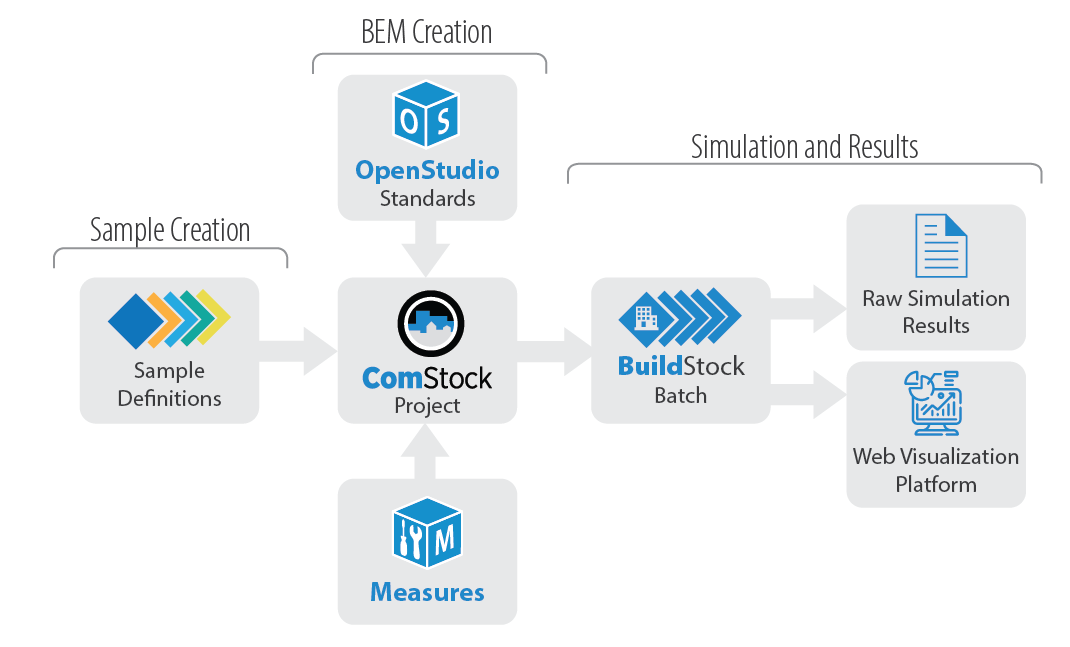
\includegraphics[width=\textwidth]{figures/comstock_workflow.png}
  \caption[Flowchart of the ComStock workflow]{Flowchart of the ComStock workflow.}
  \label{fig:comstock_workflow}
\end{figure}

\pagebreak

ComStock accomplishes its goal of accurately representing the U.S. building stock through a three-part workflow process: \begin{enumerate}
    \item ComStock creates samples that represent the U.S. commercial building stock.
    \item These samples are translated into BEMs and modified to represent either the baseline U.S. commercial building stock or an altered version thereof (i.e., modeling the impact of an efficiency or electrification measure).
    \item The physics-based BEMs are evaluated through an energy simulation engine that uses high-performance computing to simulate each model. The resulting data are made available to a wide range of stakeholders.
\end{enumerate}

\section{ComStock Sample Definitions}
\label{sec:sample_definitions}

ComStock uses a number of publicly and privately available databases that define what buildings exist, where they are located, when they were built, and with what characteristics they have. The characteristics include (but are not limited to) floor area, HVAC system type, and window type, as well as building-type-specific characteristics such as number of beds (for hospitals) or number of students (for educational institutions). When assembled, these data sets provide the basis for representing the U.S. commercial building stock.

The input data sets used to develop ComStock are often the result of extensive, highly capital-intensive data collection efforts. Some of the data sets purchased for this work are subject to data retention clauses that require deletion of the raw data after the contractual use has been completed. Given these contractual agreements, ComStock typically aggregates and joins with other data sets to generate distributional estimates of relationships between key characteristics. These input distributions are the first step in generating samples for ComStock.

Translating the input distributions into individual samples, or combinations of characteristics, requires a sampling process. Currently, ComStock assembles all input distributions as an $n$-dimensional joint probability distribution, which is then sampled using a space-filling sampling algorithm. The goal of the sampling algorithm is to minimize the largest void, or ``gap,'' between individual samples.

Each sample generated by the sampling algorithm defines the input characteristics for a single BEM. This results in hundreds of thousands of BEMs (millions when alterations to the building stock are also considered). Each of these BEMs must be created through automated model-generation scripts (discussed in Section~\ref{sec:openstudio_standards}) and evaluated via a BEM physics engine (discussed in Section~\ref{sec:buildstockbatch}). Additionally, it is often necessary to consider the impact of alterations or retrofits to the building stock---the development and use of Measures are discussed in the following section (Section~\ref{sec:measures}).

\section{Measures for ComStock}
\label{sec:measures}

A major advantage of physics-based models is their ability to change the inputs and evaluate the effect on the outputs. For ComStock, such changes are primarily evaluated using Energy Efficiency Measures or Electrification Measures. Although the word \emph{measure} has a generally accepted meaning in the energy efficiency industry, when capitalized henceforth, \emph{Measure} indicates a script that can be executed on the ComStock BEMs to alter the model inputs. A collection of Measures is a collection of scripts that allow various alterations---such as energy efficiency interventions, electrification interventions, or demand-response strategies/technologies---to be applied across the 350,000 BEMs that comprise a national run with ComStock. These automated alterations are a key aspect of ComStock's value proposition.

Throughout ComStock's development, various Measures have been developed for specific projects. These include Measures developed to support the Los Angeles 100\% Renewable Energy Study (LA100), the Advanced Building Construction Typology Report, and, in ComStock's infancy, the Electrification Futures Study. Currently, the ComStock team is developing a more robust and generalized set of Measures that will be published. These Measures are still in development, but at minimum will include efficiency and electrification Measures.

A key element of Measures is the interconnected nature of the intervention and the BEM representation of building systems and technologies. As an example, when modeling an intervention that adds an economizer to all rooftop units without an economizer, the modeling workflow relies on (a) the Measure identifying which rooftop units already have an economizer, and (b) the Measure updating the BEMs that do not have an economizer.

In the case of a Measure that electrifies forklifts in warehouses, however, two issues arise. First, none of ComStock's sample definition characteristics provide information on which warehouses (or other building types) this measure is applicable to, or to what degree. Second, there is no disambiguation of forklift load vs. other internal load in ComStock. As such, any Measure that attempts to implement this intervention has to rely on scaled measurement and verification or market research studies. In both cases, the estimates may be accurate, but it is difficult to tie the impact to any fundamental characteristic of the model and represent the variability of the impact across buildings. Although this does not invalidate the value of such a measure, it is important to differentiate measures that fit into ComStock's sample definitions and OpenStudio-Standards' workflow from those that are ``bolted on'' post-hoc.

\section{OpenStudio-Standards}
\label{sec:openstudio_standards}

OpenStudio-Standards is an open-source modeling library that defines the detailed inputs of a BEM based on simple input values. It contains the software needed to add all building systems for each vintage of every building type. This software is primarily based on the building energy code at the time of construction/retrofit. It contains the software code needed to add all building systems for each vintage of every building type, primarily based on building energy code followed by the building at time of construction/retrofit. This capability is paired with a set of space types that represent the loads of a specific building type to allow for complete model definition.

OpenStudio-Standards was originally developed to help automate the process of creating energy code baseline BEMs. This allowed for more consistent creation of baseline models for efficiency incentive programs. Throughout the development and calibration of ComStock, these code-minimum assumptions have been altered to better reflect the building performance seen in measured data sources. In some cases, this has resulted in components being defined on a non-code basis (e.g., LEDs), whereas in other cases, calibration has resulted in alterations to the nominal assumptions in code-minimum definitions. These alterations are discussed in detail in the relevant subsections of Section~\ref{chap:4_modeling}.

OpenStudio-Standards was not originally developed for ComStock and is used for many other purposes. The standards represent the collaborative work of many researchers at Lawrence Berkeley National Laboratory, Pacific Northwest National Laboratory, and Oak Ridge National Laboratory.

\section{ComStock Project}

A ComStock project includes a baseline building stock definition and a selection of Measures. For example, a ComStock project that analyzes the building envelope savings potential for the state of Colorado would include all building samples in Colorado and Measures that capture several efficiency levels for walls, roofs, and windows. The results of this project would identify the energy impacts of bringing Colorado commercial building envelopes up to code and/or above code.

Results for a ComStock project are relative to a fixed point in the lifespan of the building stock. For example, ComStock currently represents the building stock as it looked in 2018. Results assume overnight adoption of changes to the building stock. In reality, large-scale changes to the building stock take many years, and the building stock evolves during that process. If either the baseline building stock characteristics or the measures being considered change significantly, careful consideration of the applicability of results is needed. In many cases, the changes in the point in time and the measures being considered will not significantly change the results. However, in some cases, a rapidly evolving understanding of technology performance and saturation, or increasingly refined questions, will trigger the need for updated or refined analyses. For example, state-of-the-art air-source heat pump characteristics may change rapidly, making results from a ComStock project using older technology assumptions obsolete.

\section{BuildStockBatch}
\label{sec:buildstockbatch}

BuildStockBatch is a software library that executes ComStock and ResStock projects. ResStock is a residential building sector model and shares many workflow components with ComStock.  BuildStockBatch is typically used by NREL researchers on NREL's high-performance computing system, Eagle. However, the ResStock team has developed and demonstrated an Amazon Web Services (AWS)-based workflow that can be used by entities without access to the U.S. Department of Energy's (DOE's) high-performance computing system. BuildStockBatch can run up to tens of millions of simulations for a given ComStock (or ResStock) project. Although the number of simulations in these projects can vary greatly, BuildStockBatch scales by distributing simulations across a number of servers. The number of servers increases in proportion to the number of simulations, ranging from a few servers to hundreds of servers. After each server completes its requested simulations, it pushes the results to a remote file-system-based database.

Currently, BuildStockBatch utilizes an Eagle high-performance computing workflow for ComStock. In the future, ComStock expects to provide a proof-of-concept BuildStockBatch implementation that uses AWS to execute a ComStock simulation. It is not yet clear whether funding will be allocated to support this workflow's use by third-party users, but the AWS-enabled code base will be publicly available when developed.

\section{Raw Simulation Results}
\label{rawsimulationresults}
The simulation results from national ComStock releases are transferred to an AWS bucket provided by the Open Energy Data Initiative (OEDI) Data Lake partnership with AWS. This bucket contains several versions of the raw results. It contains the OpenStudio BEMs (.osm files) used to represent each sampled building. It also provides each building sample's simulated energy consumption results on a 15-minute basis, per end use, per Measure upgrade. These files are stored such that they can be queried using AWS's Athena service. Finally, the annualized results are provided on a baseline/upgrade basis, where each Measure upgrade defined in the ComStock project has its own annualized result file.

\section{Web-Based Visualization Platform}
\label{dataviewer}
ComStock and ResStock utilize a shared platform for data visualization. In most cases, users are looking for the sum or average load profile of all buildings of a given type in a given geographic area. These are referred to as ``aggregate'' load profiles. The visualization platform, which can be found at \href{comstock.nrel.gov}{comstock.nrel.gov}, provides users with an interface to interact with both annualized and 15-minute-interval data segmented by geography and building characteristic. As previously discussed, ComStock does not providet results that represent specific buildings, but rather aims to represent the distribution and variability of the building stock across the United States. Users who interact with \href{comstock.nrel.gov}{comstock.nrel.gov} generally have a more consistent and beneficial experience than those who interact with individual sample results. The results are available for several weather years and several different geographic resolutions. It is important to note that, at present, the more refined the geographic resolution, the less confidence should be placed in the results. This is because fewer samples will have been generated to approximate the relevant stock.
\chapter{Building Characteristic Sampling}

There are three steps to creating the sample of buildings modeled by ComStock. The first step creates estimates of the sizes, ages, types, and locations of the buildings that exist throughout the United States.  The second step is characteristic estimation, which is detailed in Section~\ref{chap:4_modeling}. This step defines the additional characteristics of buildings that determine energy consumption and performance. These characteristics are mostly derived from different data sources than those used in the stock estimation step, although they often depend on stock estimation parameters such as building type or age. The third step is sampling the multidimensional probability space to generate a collection of input parameters, or samples. The final samples give an accurate estimation of the commercial building stock at large while not attempting to model any individual building exactly. Stock estimation and sampling are described further in this section, but the majority of the characteristics are discussed in Section~\ref{chap:4_modeling}.

\section{Stock Estimation}

Any estimate of the energy consumption of the U.S. commercial building stock relies heavily on an estimate of how much floor area of each type of building exists in each part of the country. As shown by CBECS \citep{eia2012cbecs} and others, energy consumption of commercial buildings predominantly scales with floor area, not with building count. An accurate estimate of building floor area is therefore a critical input into any stock modeling tool focused on energy or energy-related metrics.

A secondary issue is the type of building associated with each floor area. Although accurately estimating the total floor area of commercial buildings is necessary, it is not sufficient, as building type also has an impact on energy use intensity (EUI), measured in units of energy use per square foot per year. As an example, a large office with a data center would be expected to have a dramatically higher electric load per square foot than an unconditioned warehouse.

The goal of the stock estimation process is to identify the type, floor area, and location of buildings across the United States. This task is complicated by a number of factors, including data sources that are inconsistent across the United States. However, floor area estimation is central to ensuring that ComStock is accurate for its intended use cases. ComStock takes a three step approach towards achieving an accurate estimate. To begin, national data sources are assembled to present overlapping (and often conflicting) reports of the U.S. commercial building stock. Second, the buildings reported by the various data sources are assigned a consistent set of type descriptors---e.g., large office or secondary school. Finally, the various data sets are amalgamated to create a final, consistent data set that is used in the sampling process.

\subsection{Data Sources}

ComStock's stock estimation is assembled using several data sources. The primary data sources are CoStar, a commercial building real estate intelligence broker, and Homeland Infrastructure Foundation-Level Data (HIFLD), a Department of Homeland Security database that provides cross-agency information on critical infrastructure assets across the United States. Both of these data sets, due to their business-/mission-driven use cases, tend to have very high accuracy for the buildings they represent. However, the major downside of both data sources is that the buildings they do not collect data on are not represented in any manner. While this is challenging, it is easier to adjust/correct for this sparsity than to use other data sets in which buildings are incorrectly and inconsistently represented.

CoStar is a ``leading provider of commercial real estate data and marketplace listing platforms. Its data offerings contain in-depth analytical information on over five million commercial real estate properties related to various subsections, including office, retail, multifamily, healthcare, industrial, self-storage, and data centers'' \citep{costar_10k}. CoStar's data is driven by commercial leases and commercial sales data, and is updated with millions of dollars' worth of research per year. CoStar's data set is not always complete, both in terms of geography and building type. For example, building types that are rarely bought and sold, such as schools and major hospital complexes, are less likely to be represented in CoStar's database.

HIFLD is a set of data tables assembled by the U.S. Department of Homeland Security to support critical infrastructure awareness, disaster recovery, and various other uses. Their databases include information on critical infrastructure facilities such as refineries and military bases, but also include information on schools (which are often used as disaster assistance centers) and hospitals. This is particularly useful, as these are two of the key building types that are less likely to be represented in CoStar. Although the schools data set provided by HIFLD always provides information on the number of students enrolled in a given school (which is used as a proxy to determine the floor area of the school when not otherwise available), the hospital table fails to report the number of beds in a given hospital (which is likewise used to scale floor area) in approximately half the states in the United States. In these cases, data from states that do report this information is generalized and used to infer the floor area in states without data.

Although both of these data sets provide excellent coverage of buildings they consider, they do not provide full and complete coverage of commercial buildings across the United States. Of particular note, using these two data sources results in an estimate of U.S. commercial buildings that differs from that published by CBECS. The ComStock team, after significant discussion, has decided to treat the CBECS estimate of the floor area of each building type as a truth data set. Following the sampling of the CoStar and HIFLD data sets, the CBECS estimates are used to ``true up'' the numbers on a national basis. As a result, ComStock's floor area estimates match CBECS' by building type on a national basis. Although other truth data sources were considered, CBECS' centrality to all commercial energy use estimation made it the obvious and consistent choice for estimating the U.S. commercial building stock's energy use.

\subsection{Building Type Assignments}

Building type definitions frequently do not match across data sources. This is particularly noticeable in the case of CoStar, CBECS, and DOE prototype buildings data sources. The DOE prototype building models, discussed further in Section~\ref{sec:building_type_meta}, defines specific combinations of space types as ``building types,'' which are then used by ComStock. The building types represented by the DOE prototype building models were decided on during the development of their precursors, the DOE reference building models \citep{doe_reference_buildings}. As such, ``translating'' building types across data sources introduces a layer of complexity. 

ComStock maps the building type definitions from each data source to a specific building type from the DOE prototype buildings to maximize consistency. While these mappings are imperfect, they represent the best efforts of the ComStock team to capture the unique energy-related characteristics of different building types within the modeling framework created and used by DOE over the last 15 years. Table \ref{tab:building_types} shows the mapping from the CoStar building types and HIFLD tables to the DOE prototype buildings, and from the DOE prototype buildings to CBECS' Principal Building Activity Plus.

\begin{table}
\centering
\small
\caption[Building Type Mapping Across Data Sources]{Building Type Mapping Across Data Sources}
\label{tab:building_types}
\begin{tabular}{|p{4.25cm}|p{3.5cm}|p{3.25cm}|p{4.25cm}|}
\hline
\textbf{CoStar Building   Type}                                & \multicolumn{1}{l|}{\textbf{HIFLD Table}}                & \textbf{DOE Prototype and ComStock Building Type}                               & \textbf{CBECS Principle Building Activity Plus }         \\ \hline
Retail:   Bar                                         & \multirow{2}{*}{Not applicable}                 & \multirow{2}{*}{Full service restaurant}  & Restaurant/cafeteria                            \\ \cline{1-1} \cline{4-4} 
Retail: Restaurant                                    &                                                 &                                           & Bar/pub/lounge                                  \\ \hline
\multicolumn{1}{|l|}{Not applicable}                  & \multicolumn{1}{l|}{Healthcare: Hospitals}      & Hospital                                  & Hospital/inpatient health                       \\ \hline
Hospitality: Hotel                                    & \multirow{12}{*}{Not applicable}                & \multirow{2}{*}{Large hotel}              & \multirow{2}{*}{Hotel}                          \\ \cline{1-1}
Hospitality: Hotel casino                             &                                                 &                                           &                                                 \\ \cline{1-1} \cline{3-4} 
Office: Industrial live/work   unit                   &                                                 & \multirow{6}{*}{Office}                   & Administrative/professional office              \\ \cline{1-1} \cline{4-4} 
Office: Office live/work unit                         &                                                 &                                           & Bank/other financial                            \\ \cline{1-1} \cline{4-4} 
Office: Office/residential                            &                                                 &                                           & Government office                               \\ \cline{1-1} \cline{4-4} 
Retail: Bank                                          &                                                 &                                           & Medical office (non-diagnostic)                 \\ \cline{1-1} \cline{4-4} 
Flex                                                  &                                                 &                                           & \multirow{2}{*}{Other office}                   \\ \cline{1-1}
Office: Service                                       &                                                 &                                           &                                                 \\ \cline{1-1} \cline{3-4} 
Health care: Rehabilitation   center                  &                                                 & \multirow{4}{*}{Outpatient}               & \multirow{2}{*}{Medical office (diagnostic)}    \\ \cline{1-1}
Health care: Skilled nursing   facility               &                                                 &                                           &                                                 \\ \cline{1-1} \cline{4-4} 
Office: Medical                                       &                                                 &                                           & \multirow{2}{*}{Clinic/other outpatient health} \\ \cline{1-1}
Health care                                           &                                                 &                                           &                                                 \\ \hline
\multicolumn{1}{|l|}{\multirow{2}{*}{Not applicable}} & \multicolumn{1}{l|}{Education: Public schools}  & \multirow{2}{*}{Primary/secondary school} & Elementary/middle school                        \\ \cline{2-2} \cline{4-4} 
\multicolumn{1}{|c|}{}                                & \multicolumn{1}{l|}{Education: Private schools} &                                           & High school                                     \\ \hline
Retail: Fast food                                     & \multirow{24}{*}{Not applicable}                & \multirow{2}{*}{Quick service restaurant} & \multirow{2}{*}{Fast food}                      \\ \cline{1-1}
General retail: Fast rood                             &                                                 &                                           &                                                 \\ \cline{1-1} \cline{3-4} 
Retail: Department store                              &                                                 & \multirow{4}{*}{Retail}                   & \multirow{2}{*}{Retail store}                   \\ \cline{1-1}
Retail: Freestanding                                  &                                                 &                                           &                                                 \\ \cline{1-1} \cline{4-4} 
Retail: Garden center                                 &                                                 &                                           & \multirow{2}{*}{Other retail}                   \\ \cline{1-1}
General retail: Freestanding                          &                                                 &                                           &                                                 \\ \cline{1-1} \cline{3-4} 
Hospitality: Motel                                    &                                                 & \multirow{2}{*}{Small hotel}              & \multirow{2}{*}{Motel or inn}                   \\ \cline{1-1}
Hospitality                                           &                                                 &                                           &                                                 \\ \cline{1-1} \cline{3-4} 
Flex: Showroom                                        &                                                 & \multirow{7}{*}{Strip mall}               & \multirow{7}{*}{Strip shopping mall}            \\ \cline{1-1}
Retail: Storefront                                    &                                                 &                                           &                                                 \\ \cline{1-1}
Retail: Storefront   retail/office                    &                                                 &                                           &                                                 \\ \cline{1-1}
Retail: Storefront   retail/residential               &                                                 &                                           &                                                 \\ \cline{1-1}
Specialty: Post office                                &                                                 &                                           &                                                 \\ \cline{1-1}
Retail                                                &                                                 &                                           &                                                 \\ \cline{1-1}
General retail                                        &                                                 &                                           &                                                 \\ \cline{1-1} \cline{3-4} 
Flex: Light distribution                              &                                                 & \multirow{9}{*}{Warehouse}                & \multirow{3}{*}{Distribution/shipping center}   \\ \cline{1-1}
Flex: Light manufacturing                             &                                                 &                                           &                                                 \\ \cline{1-1}
Industrial: Distribution                              &                                                 &                                           &                                                 \\ \cline{1-1} \cline{4-4} 
Industrial: Service                                   &                                                 &                                           & \multirow{3}{*}{Nonrefrigerated warehouse}     \\ \cline{1-1}
Industrial: Showroom                                  &                                                 &                                           &                                                 \\ \cline{1-1}
Industrial: Truck terminal                            &                                                 &                                           &                                                 \\ \cline{1-1} \cline{4-4} 
Industrial: Warehouse                                 &                                                 &                                           & \multirow{3}{*}{Self-storage}                   \\ \cline{1-1}
Specialty: Airplane hangar                            &                                                 &                                           &                                                 \\ \cline{1-1}
Specialty: Self-storage                               &                                                 &                                           &                                                 \\ \hline
\end{tabular}
\end{table}

It is important to note that only one of either the CoStar or HIFLD data is used to represent each type of DOE prototype building---that is, no building type is pulled from both data sets. This ensures that any errors that exist in either data set are independently corrected by the CBECS normalization. According to CBECS' estimation, the amalgamation of these three data sets accounts for 64\% of the energy use and 62\% of the floor area of commercial buildings in the United States. The remaining 36\% of energy use not represented  is due to several CBECS building types that are not included in ComStock yet such as grocery stores and religious worship. Figure \ref{fig:types_not_represented} shows the building types not represented in the ComStock model, on a CBECS Principal Building Activity Plus basis, and their relative contribution to the commercial building energy use in the United States. As can be seen in the figure, college/universities represent the largest un-modeled building classification by energy use, followed by religious institutions, mixed-use offices, grocery stores, nursing homes, and recreational buildings. Although these building types all consume energy, the ComStock team does not have sufficient information to make a reasonable estimate of their energy use, either annually or on a time-series basis, using the approach discussed in Section \ref{sec:space_type_ratios}.

\begin{figure}
  \centering
  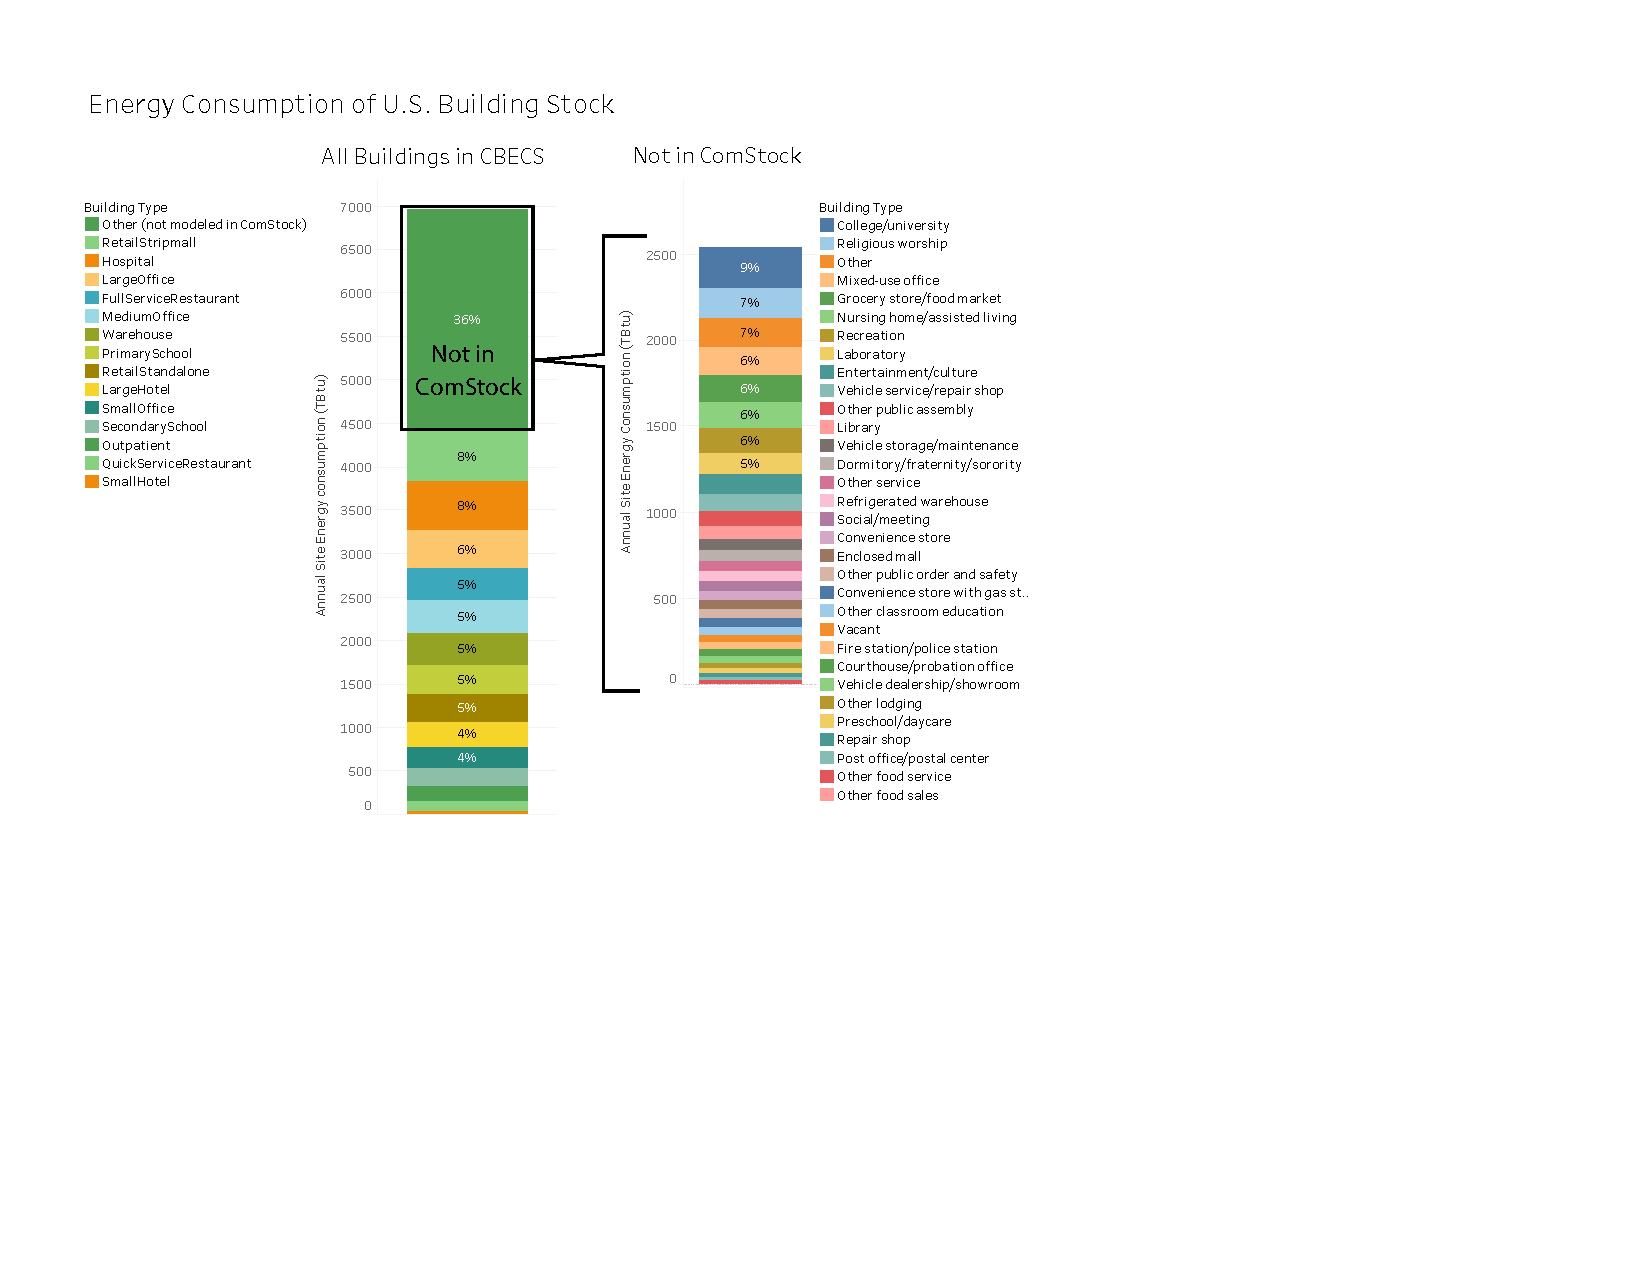
\includegraphics[
        page={1}, 
        trim={1cm 7cm 10cm 1cm}, clip, % L B R T
        width=\textwidth] {figures/CBECS_2012_comstock_coverage.pdf}
  \caption[CBECS building types not covered by ComStock]{CBECS Principal Buildings Activity Plus building types not covered by ComStock on an energy use basis.}
  \label{fig:types_not_represented}
\end{figure}

DOE prototype building type is used to represent a significant amount of the U.S. building stock but is also not used in many cases due to concerns regarding its accurate representation of specific building sub-types. The following list discusses each building type, and what buildings it does and does not represent, as understood by ComStock's developers.

\newpage

\begin{description}
\item [Full Service Restaurant] Both sit-down restaurants and bars are included in this category, as both typically require significant cooking and sanitation equipment for their operation.
\item[Hospital] Hospitals, wherever possible, are disambiguated from outpatient clinics through the existence of around-the-clock medical facilities. This is not possible in many states, in which case the differentiation is based on available CoStar data.
\item[Large Hotel] Large hotels are differentiated from small hotels on the basis of conference or casino spaces. Hotels that have major facilities for conferences, events, or gambling are classified as large hotels.
\item[Offices] Offices are divided up into three subsets: small, medium, and large. Each type of office is based on the thresholds used by American Society of Heating, Refrigerating and Air-Conditioning Engineers (ASHRAE) Appendix G \citep{ashrae_901_2010}, which include both size and number of stories. In the case of large offices, there are additional probability distributions that determine what percent (if any) of the office is a data center.
\item[Outpatient] Outpatient facilities, as represented in ComStock, include non-hospital medical centers, rehabilitation centers, and medical offices.
\item[Primary School] The primary school type is used to represent all schools that do not include secondary or post-secondary education, i.e., grades 9 and beyond. Schools that provide education for pre-secondary to post-secondary students (e.g., grades 5--12) are classified as secondary schools. This grouping means that any daycare facilities classified as schools by HIFLD are included as primary schools, unless the facilities also support secondary students.
\item[Quick Service Restaurant] Quick service restaurants consist entirely of fast food restaurants.
\item[Retail] This category predominantly features large national retailers, excluding grocery stores. This includes big box stores, garden centers, department stores, and any other freestanding retailers that do not include a significant grocery section.
\item[Secondary School] Secondary schools incorporate all schools that offer instruction to pupils in grades 9--12. No post-secondary institutions (e.g., community colleges and universities) are represented by ComStock unless they fall into another building type defined herein.
\item[Small Hotel] Small hotels encompass all hotels that do not have significant spaces for conferences, meetings, or gambling.
\item[Strip Mall] Strip malls encompass all multi-tenant retail buildings, as well as single-tenant buildings that are not classified as large retailers, such as post offices, showrooms, etc. These buildings have additional probability distributions that determine how much of the building floor area (if any) is a restaurant. This is critically important, as restaurants have a far higher EUI and as a result can cause strip malls to have far higher energy uses than would otherwise be expected in a stand alone retail building.
\item[Warehouse] Warehouses are perhaps the most differentiated building type in the commercial building stock. They are represented in ComStock as a conjunction of office spaces and high-bay spaces. This building type is used to model distribution centers, light manufacturing, and some showroom and truck terminal spaces, as well as airplane hangars, service depots, and self-storage centers. The spaces encompass a large number of functions; however, it is difficult to differentiate these spaces when examining national databases of building stock characteristics. This makes further disambiguation of these buildings impossible without additional data sources.
\end{description}

\subsection{Data Amalgamation for Sampling} \label{sec:3.1.3data amalgamation for sampling}

The data from CoStar and HIFLD were converted from individual building data points to probability distributions for geographic areas due to data retention clauses. 

The ComStock team tagged all individual buildings with a climate zone and a county to convert the county-level locations of buildings within the United States into a probability distribution. From this data, one distribution was created: the likelihood of a building in the United States being located in a given climate zone. In this distribution, there is a much higher likelihood of being located in a heavily populated climate zone (like 4A, which includes much of NJ, DC, MD, DE, VA, etc.) than a sparsely populated climate zone (like 8, which includes only part of AK). Next, for each climate zone, another distribution was created: the likelihood of a building being located in each county within that climate zone. In these distributions, there is a much higher likelihood of being located in a heavily populated county than a sparsely populated county. These two sets of distributions allow any ComStock sample to be assigned a climate zone and a county  prior to any additional characteristics being calculated.

The next characteristic to be described as a probability distribution was the building type. Based on the combined CoStar and HIFLD data sets, the likelihood of a building being of a specific building type was calculated for each county in the United States. In some cases, the county in question had an insufficient number of buildings in CoStar and HIFLD to create a realistic distribution. In these cases, the county was instead assigned a distribution of building types based on all the buildings in the state. This is not frequently required for building type, but is more common for floor area, vintage, and number of stories (discussed next).

Probability distributions for three additional characteristics were created using the HIFLD and CoStar data sets: floor area, vintage, and number of stories. CoStar's database has excellent coverage of floor area of a building as a function of county and building type, good coverage of vintage (the year the building was constructed), and reasonable coverage of the number of stories. HIFLD, on the other hand, has good information on vintage, but not on floor area or the number of stories. For floor area, inferences were based on the number of students enrolled (for schools) and the number of beds (for hospitals). Where information on the number of beds was missing, the aggregate distribution for the United States was used to infer the floor area. The number of stories was estimated based on the inferred floor area for each hospital/school. These estimates, as well as the estimates provided by the CoStar data, were used to create distributions for each building type's characteristics on a county basis. There were several cases in which one or more characteristics could not be accurately estimated for a building type/county pair. In these cases, the aforementioned approach of using the state-level distribution was employed.

The approach employed is mathematically accurate. However, the downside to using building count when creating probability distributions is that a high sample count is required to ensure that less common but highly impactful buildings, such as buildings over one million square feet, are well represented. For example, if a county contains 100 retail stores with a floor area of 1,000 square feet each (for a total of 100,000 square feet) and one retail store (perhaps a mall) of one million square feet, the large retail store would be expected to use roughly ten times (1,000,000 square feet/ 100,000 square feet) the energy of all of the smaller retail stores put together. With the current count-based approach, around 100 samples would need to be generated from this distribution to ensure that the one million square foot retail store was represented in the model. Although the impacts of this are minimal at a higher geographic level, it is a known weakness of the current approach.

\section{Characteristic Estimation} \label{Characteristic Estimation}

The variability of the commercial building stock begins with building type and location, but extends to include a variety of additional factors. These include schedule diversity, installed equipment type, age of installed equipment, and building code. Each of the characteristics associated with these categories are discussed at length in Section \ref{chap:4_modeling}, and overviews of each are provided below.

Schedule diversity is a key source of variability in the U.S. commercial building stock. Some buildings operate on a 24/7 basis, but the percentage varies drastically by building type---i.e., there are very few primary schools throughout the United States that are ``on'' 24 hours per day, let alone 365 days per year. There is also monthly/seasonal variability in a few building types, most notably schools and hotels. Although many of the buildings have lower occupant- or schedule-driven loads during various periods, some do not (e.g., schools that offer summer school). The nuances of this variability are represented in the schedule-driven characteristic distributions.

Equipment characteristics can make a significant difference in the energy consumption of a building through differences in efficiency, fuel type, and the presence or absence of certain types of equipment. ComStock represents this variability by accounting for the fuel type variability within a given state. This allows ComStock to calculate the likelihood of various heating, ventilating, and air-conditioning (HVAC) system types as a function of building type and fuel type. As part of this calculation, systems that do not provide cooling are considered, particularly in the case of warehouses. The fuel type distribution is also used as an input to the selection of water heating equipment.

The third major category of variability is equipment vintage. In most cases, this category is driven by the age of the building. Equipment within a building is generally updated and replaced over time for reasons such as remodeling or equipment failure. As discussed in Section~\ref{sec:system_turnover_and_eul}, there is a great degree of variability in equipment lifespans, which leads to variability in the current equipment installed in buildings of a given year of construction. The age of the equipment (or, put another way, the year of manufacture/sale of the equipment) plays a large part in a buildings' efficiency. In some cases, such as buildings built within the last 5--10 years, it is unlikely that many of the building systems have been replaced. The equipment distribution, which is conditioned on the building's year of construction, reflects these nuances.

Finally, building energy codes have an impact on the efficiency of components installed within a building. Building energy codes set the minimum efficiency levels for various building components, but code adoption is not uniform across the United States. As discussed in Section~\ref{sec:energy_code}, the building code in force at the time of replacement/installation of a building component is a key driver of its efficiency.

\section{Publication of Building Characteristic Probability Distributions}
Some of the distributions described above cannot be published for contractual agreement reasons, but certain distributions can be published. The ComStock team has generated tab-separated values (tsv) files containing probabilities and dependencies. See Table \ref{tbl:distro_tbl} for the full list of building characteristic probability distributions. More detail on each building characteristic is provided later in this report.

\begin{center}
\small
\begin{longtable}{|p{1.3in}|p{1.5in}|p{1.5in}|p{1.5in}|}
\caption[Building Characteristic Distributions]{Building Characteristic Distributions Included in the ComStock Sampling Process, Including Probabilistic Dependencies and Descriptions} \\ \hline
\label{tbl:distro_tbl}
\textbf{Building Characteristic} & \textbf{Description} & \textbf{Data Source} & \textbf{Conditional On} \\ \hline
\endfirsthead
\multicolumn{4}{c} {{\bfseries \textit{Continued from previous page}}} \\ \hline
\textbf{Building Characteristic} & \textbf{Description} & \textbf{Data Source} & \textbf{Conditional On} \\ \hline
\endhead
Simulation Year                                                 & Year used in simulations                                                       &                                                            &                                                                                                      \\ \hline
Climate Zone                                                    & Climate zone as defined by American Society of Heating, Refrigerating and Air-Conditioning Engineers (ASHRAE) Standard 169--2006                            & CoStar                                                      &                                                                                                      \\ \hline
County                                                          & County FIPS code (includes state specification)                                & CoStar                                                      & Climate Zone                                                                                         \\ \hline
State                                                           & State FIPS code                                                                & CoStar                                                      & County                                                                                               \\ \hline
Building Type                                                   & Primary building type of model                                                 & CoStar                                                      & County                                                                                               \\ \hline
Building Rentable Area                                          & Building total floor area                                                      & CoStar                                                      & County, Building Type                                                                                \\ \hline
Census Region                                                   & Census region                                                                  & CoStar                                                      & State                                                                                                \\ \hline
Year of Construction                                            & Year in which the building was constructed                                     & CoStar                                                      & County, Building Type, Simulation Year                                                               \\ \hline
Year of Construction Bin                                        & Year bin in which the building was constructed                                 & CPUC DEER EULs                                              & Year of Construction                                                                                 \\ \hline
Energy Code in Force When Constructed                           & Energy code applicable to building when constructed                            & State Code Adoption History                                 & State, Year of Construction Bin                                                                      \\ \hline
Building Subtype                                               & If applicable, subtype of primary building type                                & NREL analysis of strip malls                                & Building Type                                                                                        \\ \hline
Ownership Status                                                & Ownership and occupant status of the building                                  & CBECS 2012                                                  & Building Type                                                                                        \\ \hline
Party Responsible for Purchase Authority                        & Entity responsible for purchasing decisions                                    & CBECS 2012                                                  & Ownership Status                                                                                     \\ \hline
Party Responsible for Operation                                 & Entity responsible for operation of the building                               & CBECS 2012                                                  & Ownership Status                                                                                     \\ \hline
Number of Stories                                               & Number of stories above grade                                                  & CoStar                                                      & County, Building Type                                                                                \\ \hline
Window-to-Wall Ratio                                            & Window-to-wall ratio                                                           & NFRC Commercial Fenestration Market Study                   & Building Type, Building Rentable Area, Energy Code in Force When Constructed                         \\ \hline
Building Shape                                                  & Building shape designation                                                     & CBECS 2012                                                  & Building Type                                                                                        \\ \hline
Aspect Ratio                                                    & Aspect ratio of building                                                       & CBECS 2012                                                  & Building Shape                                                                                       \\ \hline
Building Rotation                                               & Rotation of building relative to North                                         & CBECS 2012                                                  &                                                                                                      \\ \hline
Space Heating Fuel                                              & Principal heating fuel for the building                                        & CBECS 2012 Plus ResStock Residential Heating Fuel by County & Building Type, County                                                                                \\ \hline
Water Heating Fuel                                              & Heating fuel for service water heating                                         & CBECS 2012~                                                 & Space Heating Fuel, Building Type                                                                    \\ \hline
HVAC System Type                                                & Primary building HVAC system type                                              & CBECS                                                       & Building Type, Space Heating Fuel, Census Region                                                     \\ \hline
HVAC Nighttime Variability                                      & HVAC nighttime ventilation operation                                           & NREL end-use data analysis                                  & HVAC System Type, Building Type                                                                      \\ \hline
Weekday Operation Start Time                                    & Building weekday operation start time                                          & NREL/Lawrence Berkeley National Laboratory (LBNL) AMI analysis                                      & Building Type                                                                                        \\ \hline
Weekend Operation Start Time                                    & Building weekend operation start time                                          & NREL/LBNL AMI analysis                                      & Building Type                                                                                        \\ \hline
Weekday Operational Duration                                    & Building weekday operation duration                                            & NREL/LBNL AMI analysis                                      & Building Type, Weekday Operation Start Time                                                          \\ \hline
Weekend Operational Duration                                    & Building weekend operation duration                                            & NREL/LBNL AMI analysis                                      & Building Type, Weekend Operation Start Time                                                          \\ \hline
Thermostat Set point for Heating                                 & Heating set point during occupied hours                                         & NREL Tstat data analysis                                    & Building Type                                                                                        \\ \hline
Thermostat Setback for Heating                                  & Heating setback during unoccupied hours                                        & NREL Tstat data analysis                                    & Building Type                                                                                        \\ \hline
Thermostat Set point for Cooling                                 & Cooling set point during occupied hours                                         & NREL Tstat data analysis                                    & Building Type                                                                                        \\ \hline
Thermostat Setback for Cooling                                  & Cooling setback during unoccupied hours                                        & NREL Tstat data analysis                                    & Building Type                                                                                        \\ \hline
Wall Construction Type                                          & Building wall construction type                                                & LightBox                                                    & Climate Zone, Number of Stories                                                                      \\ \hline
Lighting Technology Size Bin                                    & Building size classification for lighting technology type                      &                                                             & Building Rentable Area                                                                               \\ \hline
Plug Load Base-to-Peak Ratio type                                & Methodology for variability of plug load amplitude                              & NREL end-use data analysis                                  & Building Type                                                                                        \\ \hline
Plug Load Weekday Base-to-Peak Ratio                             & Ratio between nominal and maximum weekday plug Load levels                      & NREL end-use data analysis                                  & Building Type, Plug Load Base-to-Peak Ratio Type                                                      \\ \hline
Plug Load Weekend Base-to-Peak Ratio                             & Ratio between nominal and maximum weekend plug Load levels                      & NREL end-use data analysis                                  & Building Type, Plug Load Base-to-Peak Ratio Type                                                      \\ \hline
Lighting Base-to-Peak Ratio Type                                & Methodology for variability of lighting load amplitude                         & NREL end-use data analysis                                  & Building Type                                                                                        \\ \hline
Lighting Weekday Base-to-Peak Ratio                             & Ratio between nominal and maximum weekday lighting load levels                 & NREL end-use data analysis                                  & Building Type, Lighting Base-to-Peak Ratio Type                                                      \\ \hline
Lighting Weekend Base-to-Peak Ratio                             & Ratio between nominal and maximum weekend lighting load levels                 & NREL end-use data analysis                                  & Building Type, lighting Base-to-Peak Ratio Type                                                      \\ \hline
Code Compliance for Building Construction                       & Building energy code compliance when first constructed                         & Assumption                                                  & State                                                                                                \\ \hline
Code Compliance for Interior Lighting                           & Building energy code compliance for latest interior lighting replacement       & Assumption                                                  & State                                                                                                \\ \hline
Code Compliance for Walls                                       & Building energy code compliance for latest walls replacement                   & Assumption                                                  & State                                                                                                \\ \hline
Code Compliance for Service Water Heating                       & Building energy code compliance for latest service water heating replacement   & Assumption                                                  & State                                                                                                \\ \hline
Code Compliance for Roof                                        & Building energy code compliance for latest roof replacement                    & Assumption                                                  & State                                                                                                \\ \hline
Code Compliance for Exterior Lighting                           & Building energy code compliance for latest exterior lighting replacement       & Assumption                                                  & State                                                                                                \\ \hline
Code Compliance for Interior Equipment                          & Building energy code compliance for latest interior equipment replacement      & Assumption                                                  & State                                                                                                \\ \hline
Code Compliance for Windows                                     & Building energy code compliance for latest window replacement                  & Assumption                                                  & State                                                                                                \\ \hline
Code Compliance for HVAC                                        & Building energy code compliance for latest HVAC replacement                    & Assumption                                                  & State                                                                                                \\ \hline
Last Replacement Year for Interior Lighting                     & Year of most recent replacement of the interior lighting system                & CPUC DEER EULs                                              & Simulation Year, Year of Construction                                                                \\ \hline
Last Replacement Year for HVAC                                  & Year of most recent replacement of the HVAC system                             & CPUC DEER EULs                                              & Simulation Year, Year of Construction                                                                \\ \hline
Last Replacement Year for Service Water Heating                 & Year of most recent replacement of the service water heating system            & CPUC DEER EULs                                              & Simulation Year, Year of Construction                                                                \\ \hline
Last Replacement Year for Walls                                 & Year of most recent replacement of the wall                                    & CPUC DEER EULs                                              & Simulation Year, Year of Construction                                                                \\ \hline
Last Replacement Year for Windows                               & Year of most recent replacement of the windows                                 & CPUC DEER EULs                                              & Simulation Year, Year of Construction                                                                \\ \hline
Last Replacement Year for Roof                                  & Year of most recent replacement of the roof                                    & CPUC DEER EULs                                              & Simulation Year, Year of Construction                                                                \\ \hline
Last Replacement Year for Exterior Lighting                     & Year of most recent replacement of the exterior lighting system                & CPUC DEER EULs                                              & Simulation Year, Year of Construction                                                                \\ \hline
Last Replacement year for Interior Equipment                    & Year of most recent replacement of the interior equipment system               & CPUC DEER EULs                                              & Simulation Year, Year of Construction                                                                \\ \hline
Code in Force for Replacement of Interior Lighting              & Energy code in force at time of last interior lighting renovation              & State Code Adoption History                                 & State, Last Replacement Year for Interior Lighting                                                   \\ \hline
Code in Force for Replacement of Windows                        & Energy code in force at time of last window renovation                         & State Code Adoption History                                 & State, Last Replacement Year for Windows                                                             \\ \hline
Code in Force for Replacement of Roof                           & Energy code in force at time of last roof renovation                           & State Code Adoption History                                 & State, Last Replacement Year for Roof                                                                \\ \hline
Code in Force for Replacement of HVAC                           & Energy code in force at time of last HVAC renovation                           & State Code Adoption History                                 & State, Last Replacement Year for HVAC                                                                \\ \hline
Code in Force for Replacement of Walls                          & Energy code in force at time of last walls renovation                          & State Code Adoption History                                 & State, Last Replacement Year for Walls                                                               \\ \hline
Code in Force for Replacement of Service Water Heating          & Energy code in force at time of last service water heating renovation          & State Code Adoption History                                 & State, Last Replacement Year for Service Water Heating                                               \\ \hline
Code in Force for Replacement of Interior Equipment             & Energy code in force at time of last interior equipment renovation             & State Code Adoption History                                 & State, Last Replacement year for Interior Equipment                                                  \\ \hline
Code in Force for Replacement of Exterior Lighting              & Energy code in force at time of last exterior lighting renovation              & State Code Adoption History                                 & State, Last Replacement Year for Exterior Lighting                                                   \\ \hline
Energy Code Followed for Building Construction                  & Energy code followed when building was constructed                             & State Code Adoption History Plus Year Built and Turnover    & Energy Code in Force when Constructed, Code Compliance for Building Construction                     \\ \hline
Energy Code Followed for Replacement of Interior Lighting       & Energy code followed when current interior lighting system installed           & State Code Adoption History Plus Year Built and Turnover    & Code in Force for Replacement of Interior Lighting, Code Compliance for Interior Lighting            \\ \hline
Energy Code Followed for Replacement of Service Water Heating   & Energy code followed when current service water heating system installed       & State Code Adoption History Plus Year Built and Turnover    & Code in Force for Replacement of Service Water Heating, Code Compliance for Service Water Heating    \\ \hline
Energy Code Followed for Replacement of Windows                 & Energy code followed when current windows were installed                       & State Code Adoption History Plus Year Built and Turnover    & Code in Force for Replacement of Windows, Code Compliance for Windows                                \\ \hline
Energy Code Followed for Replacement of Roof                    & Energy code followed when current roof was installed                           & State Code Adoption History Plus Year Built and Turnover    & Code in Force for Replacement of Roof, Code Compliance for Roof                                      \\ \hline
Energy Code Followed for Replacement of Interior Equipment      & Energy code followed when current interior equipment installed                 & State Code Adoption History Plus Year Built and Turnover    & Code in Force for Replacement of Interior Equipment, Code Compliance for Interior Equipment          \\ \hline
Energy Code Followed for Replacement of HVAC                    & Energy code followed when current HVAC system installed                        & State Code Adoption History Plus Year Built and Turnover    & Code in Force for Replacement of HVAC, Code Compliance for HVAC                                      \\ \hline
Energy Code Followed for Replacement of Walls                   & Energy code followed when current walls were installed                         & State Code Adoption History Plus Year Built and Turnover    & Code in Force for Replacement of Walls, Code Compliance for Walls                                    \\ \hline
Energy Code Followed for Replacement of Exterior Lighting       & Energy code followed when current exterior lighting system installed           & State Code Adoption History Plus Year Built and Turnover    & Code in Force for Replacement of Exterior Lighting, Code Compliance for Exterior Lighting            \\ \hline
Lighting Technology Generation                                  & Generation of lighting technology used in building                             & Lighting Market Characterization                            & Code in Force for Replacement of Interior Lighting, Last Replacement Year for Interior Lighting      \\ \hline
Window Technology Type                                          & Window technology type used in the building                                    & NFRC Commercial Fenestration Market Study                   & Energy Code Followed for Replacement of Windows, Climate Zone                                        \\ \hline
\end{longtable}
\end{center}

\section{Sampling Methodology}
The previous subsections describe the creation of building characteristic probability distributions that are in many cases are conditional on one another. These  distributions, when joined together, create a multidimensional joint probability distribution. This joint probability distribution represents the ComStock team's best estimate of the building characteristics of the commercial building stock in the United States. In order to go from the joint probability distribution to a set of discrete building samples, a sampling algorithm must be used.

Several different classes of algorithms support sampling in multidimensional probability spaces. ComStock's choice has largely been influenced by \cite{sobol_sampling}, which introduced Sobol Sequences as a low-discrepancy basis for sampling in higher-dimensional spaces. This approach attempts, with each sample, to optimally reduce the maximal space between samples. Although this approach can be implemented on an iterative basis, ComStock adopted an approach developed by \cite{sobol_lib}, which uses a bit-switching algorithm to select optimal sampling within an $n$-dimensional probability space. This approach is designed to accurately capture the full extent of the distributions with limited samples on a non-biased basis. In other words, all buildings within a type are equally weighted after sampling, rather than being reweighted as a secondary step to sampling.

The results of applying these algorithms produced 350,000 building samples. The set of characteristics for each sample defines the inputs to the ComStock BEM workflow, which creates a BEM for each sample. The characteristics of the 350,000 samples are recorded in the buildstock.csv file. The buildings described in this file provide the ComStock team's best estimate of the characteristics for a large portion of the United States' commercial building stock for use by researchers, practitioners, and consultants. For a detailed look at the accuracy of the resulting models, refer to \cite{eulp_final_report}. The building energy models for ComStock's 350,000 baseline building samples are available to download at \url{https://data.openei.org/} in the nrel-pds-building-stock data lake. See the README.md file for details.

\label{chap:3_sampling}
\chapter{ComStock Building Models}
\label{chap:4_modeling}

ComStock uses about 30 high-level, whole-building characteristics to describe each building, as discussed in Section~\ref{chap:3_sampling}. However, whole-building energy models, such as the EnergyPlus\textsuperscript{\textregistered} model used by ComStock, typically require thousands of  inputs to describe a building for simulation. The purpose of the subsequent sections is to describe the assumptions, conventions, and data sources used to transform the high-level descriptions into inputs with the level of detail needed by EnergyPlus. Although the software used to implement this transformation is critical to the workflow, the focus is on the model inputs, not on the software workflow.

One question that often arises is why more of the input assumptions documented in this section are not incorporated directly into the sampling framework described in Section~\ref{chap:3_sampling}. This is an especially common question for those familiar with ResStock\textsuperscript{\texttrademark} \citep{resstock}, the residential building stock modeling tool that ComStock is based on. After all, ResStock uses more than 100 building characteristics to describe residential dwelling units, which are arguably less complex than commercial buildings. There are two main drivers behind the decision to limit the number of building characteristics: (1) handling complexity and (2) data availability for commercial buildings.

From a complexity standpoint, there is significantly more diversity among commercial buildings than among residential buildings. At one extreme, there are buildings like large hospitals, which may be several hundred thousand square feet, encompass spaces ranging from operating rooms to cafeterias, and be served by a complex array of HVAC systems. At the other extreme, there are buildings like small standalone retail stores, which may consist of just one retail space, a small storage room, and a restroom. Accounting for the diversity in lighting power density for each space type across all commercial building types in ComStock would alone require more than 100 building characteristics, many of which would not be applicable for certain building types. Multiply this by the number of characteristics that vary between building types, and the number of building characteristics required quickly becomes untenable.

From a data availability standpoint, there is simply much less information available for commercial buildings than there is for residential buildings. This means that modeling the commercial building stock requires more assumptions than modeling the residential building stock. Compounding this lack of data is the fact that most commercial building data sources handle complexity by focusing on a single building type (e.g., offices), providing information only at the whole-building level, or providing percentages of floor area associated with a given characteristic. Rather than making engineering estimates to generate probability distributions for every building characteristic, we have chosen to make point estimates for certain parameters. Proponents of stochastic modeling may disagree with this approach, but we believe it is warranted, given the model complexity that is avoided.

The end result is that many of the intra-building characteristics of commercial buildings must be inferred from whole-building characteristics. Rather than adding these to the input layer, they are set in the process that expands these whole-building characteristics into energy model inputs.

\section{Location, Type, Age, Space Programming, Energy Code, and Change Over Time}
\subsection{Location}

ComStock has four levels of location granularity for its building models: ASHRAE Standard 169 - 2006 climate zone, census division, state, and county. During sampling, each model is first assigned a climate zone, then a county, then a state and census division. The climate zone and county probability distributions come from the CoStar and HIFLD data provided by the Homeland Security Infrastructure Program (HSIP) on a building count basis. The state and census division are assigned using a lookup table that is based on the model's sampled county. The location metadata impacts numerous characteristics in the model, such as weather file, building type, building geometry characteristics (e.g., number of stories and rentable area), and energy code applicability. Table  \ref{tab:census_division_models_table} shows the number of models used in each census division.

Additional location metadata is joined to the \emph{buildstock.csv} for use in parsing ComStock results. This includes data such as \href{https://www.census.gov/programs-surveys/geography/guidance/geo-areas/pumas.html}{Public Use Microdata Area} (PUMA), \href{https://www.energy.gov/eere/buildings/building-america-climate-specific-guidance}{Building America climate zone}, \href{https://isorto.org/}{independent system operator (ISO) region}, and \href{https://www.nrel.gov/analysis/reeds}{ReEDS balancing area}. This location metadata is joined on the \href{https://www2.census.gov/geo/pdfs/education/CensusTracts.pdf}{census tract} level. Census tracts are assigned to the \emph{buildstock.csv} using the CoStar and HSIP data.

\begin{table}[h!]
\centering
\small
\caption[Distribution of ComStock Models in Each Census Division]{Distribution of ComStock Models in Each Census Division}
\label{tab:census_division_models_table}
\begin{tabular}{|c|c|c|}
\hline
\textbf{Census Division}                                & \textbf{Count}              & \textbf{Percentage}                                     \\ \hline
East North Central                                         & 54122                 & 15.46\%      \\ \hline
East South Central                                         & 19882                 & 5.68\%      \\ \hline
Mid-Atlantic                                         & 44976                & 12.85\%      \\ \hline
Mountain                                         & 24258                & 6.93\%      \\ \hline
New England                                         & 16791                & 4.80\%      \\ \hline
Pacific                                         & 54799                & 15.66\%      \\ \hline
South Atlantic                                         & 72616                & 20.75\%      \\ \hline
West North Central                                         & 20910                & 5.97\%      \\ \hline
West South Central                                         & 41646                & 11.90\%      \\ 
\hline
\end{tabular}
\end{table}

\subsection{Building Type} 
\label{sec:building_type_meta}

The building types used by ComStock were originally defined by the DOE reference buildings, which were extended to create the prototype buildings. These building type definitions represent buildings by drawing on the applicable building code sets. Both the reference buildings and the prototype buildings have historically been used by building code organizations, include the ASHRAE 90.1 committee, to understand the potential impact of various code updates on newly constructed buildings.

Each building type is predominantly defined by a space type breakdown. For a given square footage of a ComStock building type, the fraction of the square footage of space type A (open office) vs. B (closed office) will remain the same as what they are in the DOE prototype models with two exceptions. Although these definitions are useful in the analysis of energy codes, there are several cases where they fail to provide the variability required for ComStock to provide a useful representation of the U.S. commercial building stock. There are two building types are currently represented with additional variability in space programming - large office and strip malls.

\begin{description}
\item[Large Offices] Currently, large offices have variable data-center loads in ComStock. This aligns with study data obtained through the \href{https://www.nrel.gov/docs/fy22osti/80889.pdf}{End-Use Load Profiles} (EULP) project that was used to calibrate ComStock. This results in a higher degree of EUI variability within the large office building type than would be expected with only a change in space programming, given the high energy intensity of the data center space type.
\item[Strip Malls] Strip malls often contain one or more restaurants. Strip malls with restaurants often have significantly higher EUIs than restaurant-free strip malls, which are the only kind represented by the reference and prototype models. To address the significant lack of diversity and variability in strip mall EUIs, the End-Use Load Profiles project added a variable restaurant component to strip mall models in ComStock. This results in a more realistic distribution of loads by end use across the strip mall segment.
\end{description}

\subsection{Vintage}

Vintage, as previously discussed in the sampling section~\ref{Characteristic Estimation}, is a key component of ascertaining the age and associated efficiency of building components. Vintage is determined based on information from either CoStar or HIFLD. However, in many cases, the vintage must be inferred due to a lack of available data on a county or state basis. When there is insufficient data on a county basis, state data are used, and in the few cases (typically in relation to hospitals) where state data are unavailable, national data are used.

Commercial buildings are complex in that each subsystem of the building---except perhaps walls---is expected to be replaced or updated at least once during the life of the building, without the building being reconstructed from the ground up. As such, it is critical to understand the year in which a building was first constructed in order to estimate the age (and the associated minimum energy code) as a function of the vintage. The latest year of intervention is calculated for each building component as a function of the vintage, and each of these are passed to an energy code lookup to determine which, if any, energy codes were in force.

Finally, it is important to note that vintage is especially important for recent construction. Buildings built within the last decade are unlikely to have significantly different or updated systems compared to those used at the time of construction. As a result, these buildings are a unique stock segment and have potential for cost-effective impact in the commercial building stock.

\subsection{Energy Code} % Andrew
\label{sec:energy_code}

\paragraph{Energy Code Adoption}
Some states have a statewide code, while others have codes that are determined at the city or county level. For ComStock, the adoption of an energy code is assumed to be a function of year and state. For states with no statewide code, ComStock selects the code covering the biggest cities in the state. Where a state code was not a derivative of the ASHRAE 90.1 series of codes, the most similar versions of ASHRAE 90.1 were used for that state. The exception to this is California, where the Title 24 series of codes, as represented in DEER \citep{cpuc_deer}, was used because this series of codes was known to be significantly different from ASHRAE 90.1. Most of the information used to develop the code adoption history was taken from the Building Codes Assistance Project \citep{building_codes_assistance}. Much of the building stock was constructed before energy codes were widespread. For this time period, the ``energy code'' is described as either ``DOE Ref Pre-1980,'' whose assumptions are drawn from \cite{doe_reference_buildings}, or ``DOE Ref 1980-2004,'' whose assumptions are a combination of ASHRAE 90.1-1989 and \cite{doe_reference_buildings}. Details on the specific assumptions for each energy code are described in more detail throughout this document. The code adoption history assumptions are shown in Figure~\ref{fig:energy_code}.

\begin{figure}
  \centering
  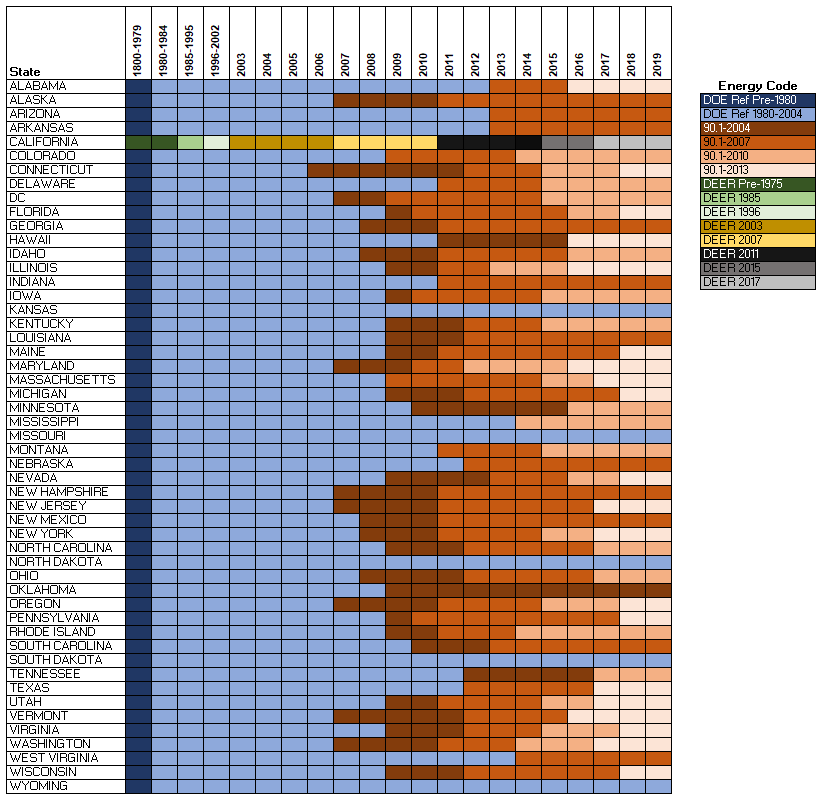
\includegraphics[]{figures/energy_code.png}
  \caption{Adoption of energy codes by state over time.}
  \label{fig:energy_code}
\end{figure}

\paragraph{Energy Code Compliance}
For this discussion, energy code compliance is defined as the extent to which a building constructed to comply with a certain energy code meets the requirements of that code. For example, a building built to comply with ASHRAE 90.1-2010 may meet all envelope requirements but fail to meet some HVAC control requirements. Unfortunately, there is little information available on commercial energy code compliance at a national level, and the information that does exist is not detailed. The status of this information is described in a detailed report \citep{icf_com_code_compliance_status} generated for EIA’s NEMS modeling effort. What we do know, both from this information and anecdotally, is that commercial energy compliance is imperfect. Some buildings and building systems exceed code, and others lag behind. Because of the data limitations, we assume that all building systems meet the requirements of the energy code that was in force in their location when the building was originally constructed and as the building systems were replaced over time. As data on major building systems become available we hope to move away from this code-compliance-based framework toward a model driven by distributions of known building characteristics.

\subsection{Building System Turnover and Effective Useful Life} % Andrew
\label{sec:system_turnover_and_eul}

We assume that all major building systems are installed when the building is constructed, and that they are replaced periodically over the lifespan of the building. Replacements may be made because of equipment failure, building remodeling, energy efficiency upgrades, etc. To model the turnover of building systems, it is necessary to understand how often these building systems are replaced, which determines how long they last in the building stock. The metric commonly used by the energy efficiency community to describe the lifespan of a measure is effective useful life (EUL). The California Public Utilities Commission defines EUL as ``an estimate of the median number of years that the measures installed under the program are still in place and operable'' \citep{cpuc_ee_manual}. In the reliability community, EUL is typically referred to as ``median time to failure'' \citep{ti_reliability_website}, whereas ASHRAE uses the term ``median service life'' \citep{ashrae_reliability_db_article}.

\par
For ComStock, the primary source of EULs is the California Public Utilities Commission (CPUC) Database of Energy Efficiency Resources (DEER) \citep{cpuc_deer}. Previous work on EULs indicates that there is wide variation in the quality of national EUL data, but it also indicates that the studies performed in DEER are generally the best available \citep{what_makes_good_eul}. The values in DEER were cross-referenced against the lifetimes used in the EIA NEMS Commercial Demand Module \citep{nems_com_demand_module} and the ASHRAE Service Life and Maintenance Cost Database \citep{ashrae_reliability_db}. Table~\ref{tab:effective_useful_life} shows the EULs assumed for different building systems in ComStock.

\begin{table}
\small
\caption[Effective Useful Life of Major Commercial Building Systems]{Effective Useful Life of Major Commercial Building Systems}
\label{tab:effective_useful_life}
\centering
\begin{tabular}{|p{3cm}|p{1cm}|p{11cm}|}
\hline
\textbf{Major Building System}                       & \textbf{EUL (Years}) & \textbf{Notes} \\
\hline
Envelope---Wall Insulation                  & 200         & This value was based on engineering judgment. DEER EULs are capped at 20 years, per CPUC policy. NEMS does not appear to model wall turnover separate from whole-building replacement.\\
\hline
Envelope---Roof Insulation                  & 200         & This value was based on engineering judgment. DEER EULs are capped at 20 years, per CPUC policy. NEMS does not appear to model roof turnover separate from whole-building replacement.\\
\hline
Envelope---Windows                          & 70          & Based on a reliability analysis of windows from the 2014 Commercial Building Stock Assessment from the Pacific Northwest. DEER uses an EUL of 20 years for window replacement, as the DEER EULs are capped at 20 years, per CPUC policy.\\
\hline
Exterior Lighting                           & 15          & This closely matches the highest EUL in DEER for outdoor lighting (16 years). NEMS does not break out exterior lighting, but all NEMS commercial lighting technology types have a 10-year EUL.\\
\hline
Interior Lighting                           & 10          & This is in line with the EULs in DEER for interior lighting, and matches the 10-year EUL for all commercial lighting technologies in NEMS.\\
\hline
HVAC                                        & 20          & The highest EUL in DEER for HVAC is 20 years. For rooftop air conditioners, which serve by far the largest portion of the building stock, NEMS uses a 21-year EUL. NEMS HVAC EULs range from 9.5 years for window AC units up to 30 years for some boilers. \citet{ashrae_reliability_db} includes 33 packaged DX rooftop units with a mean lifetime of 21 years, and appears to be the source of some NEMS HVAC lifetimes.\\
\hline
Service Water Heating (SWH)                 & 15          & The highest SWH EUL in DEER is 20 years for a tankless water heater. Most tank-based SWH equipment in DEER has an EUL of 15 years or less. NEMS non-solar SWH equipment EULs range from 10 to 15 years. \citet{ashrae_reliability_db} includes 5 gas-fired water heaters with a mean lifetime of 15 years, and 36 electric water heaters with a mean lifetime of 10 years.\\
\hline
Interior Equipment (Plug and Process Loads) & 15          & This value was based on engineering judgment and is meant to represent an average over all types of plug and process loads. If plug and process loads are addressed in future iterations, splitting the plug and process loads into information technology (IT) equipment and other equipment will be investigated, as IT equipment typically has a higher turnover rate than other process loads, such as hospital equipment or commercial kitchen equipment. NEMS includes commercial kitchen equipment with an EUL of 12 years, commercial ice machines with an EUL of 8 years, commercial vending machines with an EUL of 13.5 years, and commercial refrigeration equipment with an EUL of 10 years. \\
\hline
\end{tabular}
\end{table}

\subsubsection{Building Envelope}
For the building envelope (windows, wall insulation, and roof insulation), the DEER database was not informative, because the maximum EUL is capped at 20 years, per CPUC policy. Because of this, we sought out other sources of envelope lifetime information.

\paragraph{Windows}
As part of the DOE-funded Advanced Building Construction initiative, a team collected information on windows from a variety of commercial building surveys, including a new survey of buildings built since roughly 2010. Unfortunately, while most of the surveys did ask about windows, only one survey had enough information to perform a reliability analysis (because windows are long-lived). This survey was the 2014 Commercial Building Stock Analysis \citep{neea2014cbsa}, which covers the Pacific Northwest. This survey included information on the age of the building, whether the windows had ever been replaced (and if so, an estimate of the year of replacement), and a weighting factor to describe how each sample fit into the whole building population. From these data, we performed a reliability analysis. Figure~\ref{fig:comWindowSurvivalCurve} shows the estimated survival curve. As indicated by the black cross mark on the figure, the EUL estimate for windows is 70 years. However, the maximum lifespan extends to more than 400 years. In practice, this indicates that windows on some buildings will never be replaced.

\begin{figure}
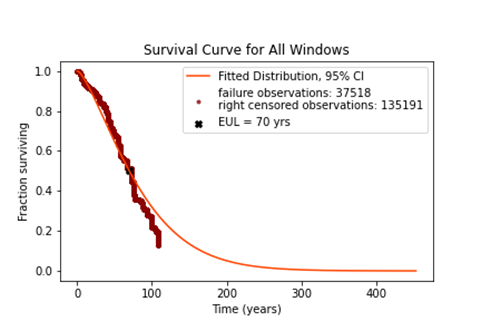
\includegraphics[width=0.6\textwidth]{figures/window_survival_curve.png}
\centering
\caption[Reliability analysis for windows in commercial buildings]{Reliability analysis for windows in commercial buildings, from 2014 CBSA \citep{neea2014cbsa}.}
\label{fig:comWindowSurvivalCurve}
\end{figure}

\paragraph{Walls and Roofs}
None of the data sources we identified included information on EULs for walls and roofs, or, more specifically, the insulation on these surfaces. DEER EULs are capped at 20 years, per CPUC policy. NEMS does not appear to model wall turnover separately from whole-building replacement. Based on engineering judgment, we selected an EUL of 200 years to indicate that for most buildings, the wall and roof insulation will not be replaced before the building is demolished.

\subsubsection{Distribution of Lifespans}
The EUL estimates in Figure \ref{fig:comWindowSurvivalCurve} represent the median lifespan for a given building system. However, not all systems will fail and be replaced after exactly that amount of time. To represent this diversity of failure rates we use a distribution.

\par
The simplest approach would be to use a normal distribution centered on the EUL. However, studies of reliability data show that this is not a good assumption; instead, these studies often use a Weibull distribution to represent lifetimes. To check whether a Weibull distribution accurately represented the lifetimes of building equipment, we performed a reliability analysis on data from the ASHRAE Service Life and Maintenance Cost Database \citep{ashrae_reliability_db}. This analysis was performed following the methodology described in an ASHRAE journal article \citep{determine_equip_life}, and was implemented using the reliability package \citep{matthew_reid_2020_3938000} in Python. Four categories of equipment with a reasonable number of entries were investigated: air handling units, boilers, chillers, and air source DX equipment (all types of each available in the database).

\begin{figure} [h!]
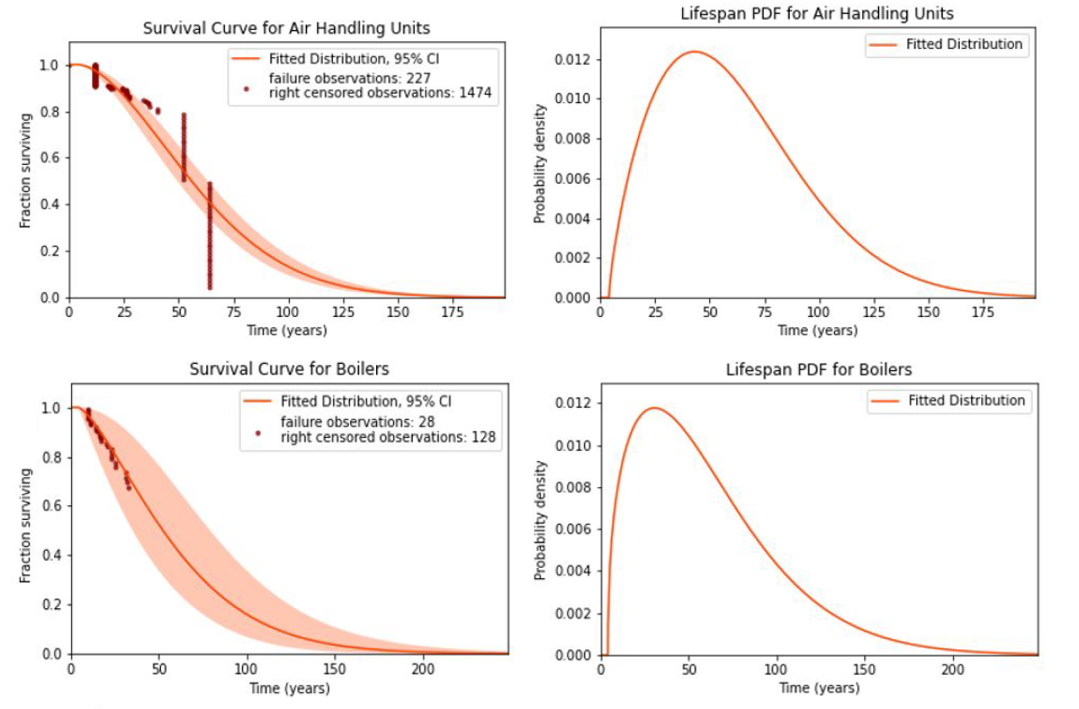
\includegraphics[width=\textwidth]{figures/ashrae_equip_lifespans2.png}
\centering
\caption[Survival curves and derived lifespan probability density functions for HVAC equipment]{Survival curves and derived lifespan probability density functions for commercial HVAC equipment.}
\label{fig:hvac_survival_curves}
\end{figure}

As shown in Figure~\ref{fig:hvac_survival_curves}, Weibull distributions are a good fit for several categories of HVAC equipment failure data. Although the ASHRAE database includes data for many different types of HVAC equipment, it was not selected as the primary source for deriving EULs for ComStock due to the limitations and biases in the database described by its creators \citep{ashrae_reliability_db_article}.
Instead, we decided to use the EUL sources described in Table~\ref{tab:effective_useful_life} and develop Weibull curve parameters around these EULs. The selected parameters are shown in Table~\ref{tab:eul_distributions}. For the 70-year EUL, the parameters came from the window reliability analysis. For the 10-, 15-, and 20-year EULs, the only constraint was to match the EUL definition: 50\% of the equipment would still be operable at the EUL. A minimum lifespan of 60\% of the EUL was selected with the assumption that although individual components of a system might fail, it is unlikely that products on the market routinely fail at a whole-building scale in only a few years. The 200-year EUL parameters were selected to represent no failure for the life of the building.

\begin{table}
\small
\centering
\caption[Commercial Equipment Lifetime Weibull Distribution Parameters]{Commercial Equipment Lifetime Weibull Distribution Parameters}
\label{tab:eul_distributions}
\begin{tabular}{|c|c|l|l|}
\hline
\textbf{EUL} & \textbf{Shape (beta)} & \textbf{Scale (alpha)} & \textbf{Shift (gamma)}    \\ \hline
10  & 1.6          & EUL / 2 = 5     & EUL * 0.6 = 6  \\ \hline
15  & 1.6          & EUL / 2 = 7.5   & EUL * 0.6 = 9  \\ \hline
20  & 1.6          & EUL / 2 = 10    & EUL * 0.6 = 12 \\ \hline
70  & 1.3          & 91              & 0              \\ \hline
200 & 1.0          & 1               & 200            \\ \hline
\end{tabular}
\end{table}

\subsection{Space Type Ratios}
\label{sec:space_type_ratios}
A space type refers to a portion of a building that has a distinct usage, purpose, occupancy schedule, thermostat set point, etc. Most buildings have multiple space types. For example, schools typically have classrooms, hallways, restrooms, cafeterias, etc. In ComStock, each building type is assumed to have a fixed ratio of various space types relative to the total building floor area. For buildings outside of California, the space type ratios were largely taken from the DOE commercial reference building models \citep{deru_2011}. For buildings in California, the space type ratios were largely taken from the DEER prototype models \citep{cpuc_deer}. There are certain building types that have altered ratios or are a mix of building types. For example in ComStock, warehouses include both unconditioned storage facilities and light manufacturing. Warehouse building subtypes alter the ratio of bulk storage. Retail strip mall buildings have different ratios of restaurant space types, with the default being 20\%. Two examples of space type ratios are shown in Table \ref{tab:space_type_ratios}. See Table~\ref{tab:space_type_ratios_all} for the space type ratios for all building types.

\begin{table}
\small
\caption[Space Type Ratio Example]{Space Type Ratio Example}
\label{tab:space_type_ratios}
\centering
\begin{tabular}{|l|l|l|c|}
\hline
\textbf{Building Type} & \textbf{Building Subtype} & \textbf{Space Type} & \textbf{Ratio} \\ \hline
Warehouse & warehouse\_default & Bulk & 66\% \\ \hline
Warehouse & warehouse\_default & Fine & 29\% \\ \hline
Warehouse & warehouse\_default & Office & 5\% \\ \hline
Retail Strip Mall & strip\_mall\_restaurant20 & Strip mall - type 1 & 20\% \\ \hline
Retail Strip Mall & strip\_mall\_restaurant20 & Strip mall - type 2 & 20\% \\ \hline
Retail Strip Mall & strip\_mall\_restaurant20 & Strip mall - type 3 & 40\% \\ \hline
Retail Strip Mall & strip\_mall\_restaurant20 & Dining & 15\% \\ \hline
Retail Strip Mall & strip\_mall\_restaurant20 & Kitchen & 5\% \\ \hline
\end{tabular}
\end{table}

\subsection{Weather Data}
ComStock can be run with two different types of weather data: typical meteorological year (TMY3) and actual meteorological year (AMY). AMY data is the data measured during a specific year, taken from weather stations such as those at airports. Because these data are from a particular calendar year, weather patterns that span large areas, such as nationwide heat waves, are captured in the data across multiple locations. Therefore, these weather patterns are captured in the outputs of ComStock. This is important for use cases where coordinated weather patterns influence loads, such as peak load impacts for bulk power grid planning. TMY3 data, in contrast, take the ``most typical'' weather for each calendar month from a 30-year historical record and stitch these months together to form a complete year. The advantage of this method is that the weather data is less influenced by an extremely hot or cold year. However, this approach does not capture wide-area weather patterns, as the month of data used varies from location to location. For a more in-depth discussion of AMY and TMY3 weather data, see \cite{eulp_method_2022}.

For geographic granularity, ComStock currently uses one weather file for each county in the United States. For counties with no weather data available (generally sparsely populated rural areas), data from the nearest weather station in the same climate zone are used. See \citep{eulp_method_2022} for a more in-depth discussion of the weather data sources, cleaning process, and assignment assumptions.
\section{Hours of Operation and Occupancy}
\label{sec:hoo}

\subsection{Hours of Operation}
\subsubsection{Overview}
Hours of operation are added to the model using operation start time and duration inputs. The start times and durations are assigned to each model through the sampling process using a set of distributions based on building type. They are then further broken down by weekday and weekend (Figure~\ref{fig:start_time} and Figure~\ref{fig:duration}). When applied to the model, the start time and duration are used to establish operating hour start and end times. These times are used to adjust the other schedules in the model (e.g., lighting, thermostat). This is achieved by stretching or shrinking the schedule on the temporal axis to align all schedules with the operating hours for the model. Note that because the weekday and weekend start times and durations are sampled independently, they are not aligned in a given building model.

\subsubsection{Hours of Operation Derivation}
We derived the hours of operation by applying the method introduced in \cite{bianchi2020modeling} to 1 year of AMI data from 6,070 buildings spread across eight utilities (the commercial schedules AMI data set). We first extracted the two-dimensional distribution of \textit{High Load Start Time} and \textit{High Load Duration} from this AMI data set, as an approximation of the schedule of hours of operations for each building type. Then, we compared this distribution with the inputs of ComStock at the start of 
 the \href{https://www.nrel.gov/buildings/end-use-load-profiles.html}{End-Use Load Profiles} (EULP) calibration.

Figure~\ref{fig:utility_building_type} lists the number of buildings for each building type from each utility's AMI data set that was considered during the EULP project. The utility data sets and names are listed in Table 10 of the EULP Final Technical Report \citep{eulp_final_report}. Among the 15 building types considered in ComStock, 14 can be found in the commercial schedules AMI data set. The only exception is secondary schools, because all schools were grouped together in the AMI data.

We compared the distribution extracted from the commercial schedules AMI data set with the inputs of ComStock at the start of the EULP calibration. The results of the small office building type are presented in Figure~\ref{fig:small_office_season} to illustrate the process, because this building type has the largest sample size in the AMI data set. We considered two day types, working day vs. non-working day, and two season definitions---one defined by month, and the other defined by daily average outdoor air temperature. The distribution of hours of operation is more diffuse in the AMI data set than in the ComStock inputs at the start of EULP calibration. Also, the duration of high load is smaller in the real AMI data than in the previous ComStock assumptions.

We explored whether and how the hours of operation are influenced by season (in Figure~\ref{fig:small_office_season}) and by utility (in Figure \ref{fig:small_office_utility}). Some differences can be observed; however, due to the modeling complexity and the desire to create a nationally applicable approach that avoids overfitting to a specific utility region, we combined the AMI data across seasons and utilities to generate a distribution of hours of operation for each building type. These new distributions were applied to ComStock in place of the existing distributions.


\subsection{Occupancy}
\subsubsection{Occupancy Density}
Occupants are assigned to individual space types as an occupancy density (people/1000 ft\textsuperscript{2}). This value, when multiplied by the total zone floor area, determines the maximum number of people in a zone.  \Crefrange{tab:food_service_occupancy_density}{tab:warehouse_occupancy_density} show the occupancy densities for all space types included in ComStock.

The majority of the ComStock occupancy density values are from the DOE prototype models. These are derived primarily from ASHRAE 62.1-2004 \citep{ashrae_62.1_2004}, with some space type densities originating from the International Building Code 2003 \citep{icc_2003}. Prototype hotel guest rooms were assumed to have 1.5 occupants each, and occupancy rates for the two hotel models were assumed to be 65\% to align with the industry average occupancy rate and \cite{jiang_2008}. Rooms were randomly assigned occupants so that 65\% of the rooms were occupied. Most of the DOE prototype hospital and outpatient space type occupancy densities were replaced with values from the 2007 Green Guide for Healthcare (GGHC), which includes typical occupancy densities for healthcare space types \citep{gghc_2007}.

\subsubsection{Occupancy Schedules}
The maximum number of people in a zone (calculated from occupancy density and zone floor area) is multiplied by an hourly occupancy schedule with values ranging from zero to one to capture the variation in building occupancy throughout the day. Figures \ref{fig:occupancy_schedules_1} and \ref{fig:occupancy_schedules_2} show the national base occupancy schedules used in ComStock, broken down by building type. For the California occupancy schedules, please see figures \ref{fig:occupancy_schedules_deer_1} and \ref{fig:occupancy_schedules_deer_2} in the Appendix. For buildings in all states except California, the base schedules are the DOE prototype occupancy schedules. California uses schedules from DEER prototype models \citep{cpuc_deer}. The DOE prototype documentation \citep{deru_2011} notes that there are few data sources that provide operating schedules for use in building energy simulations. Thus, the schedules in the prototype models were derived from two primary data sources: the Advanced Energy Design Guide Technical Support Documents \citep{jiang_2008,doebber_2009,liu_2007,pless_2007} and ASHRAE 90.1-1989 Section 13 \citep{ashrae_1989}. These schedules were then modified to account for real-world building operation, based on the experience of the engineers who created the DOE prototype models. Classroom occupancy schedules for primary and secondary schools were adjusted by factors of 0.75 and 0.70, respectively, to meet the student numbers documented in \cite{pless_2007}. Table~\ref{tab:occupancy_schedule_source} lists the data sources for occupancy schedules in each of the prototype buildings (both DOE and DEER).

These base occupancy schedules are stretched, compressed, or shifted in time to reflect the model’s assigned hours of operation. For example, the base occupancy schedule for large offices is 9 a.m.--5 p.m. (8 hours of operation). If one large office model is assigned a start time of 8 a.m. and an operating duration of 10 hours, the base schedules in the model will be stretched so that the occupied period is an additional two hours long. All schedules in the model (occupancy, lighting, thermostat, plug load, etc.) are modified in the same manner to ensure coordination between occupancy, lighting, etc.  


\subsubsection{Occupancy Activity Schedules}
Occupancy activity schedules represent the total heat gain per person, including convective, radiant, and latent heat. An internal EnergyPlus algorithm determines the fraction of the total load that is sensible and latent. The sensible portion is further divided into radiant and convective using the default fraction radiant value. DOE prototype activity levels are fixed for a given building type and range from 120--132 watts per person across the various building types. DEER prototype activity levels vary by space type and range from 117--331 watts per person. Table~\ref{tab:activity_schedule} lists the occupancy activity schedules used in ComStock.

\pagebreak

\begin{figure}
   \centering 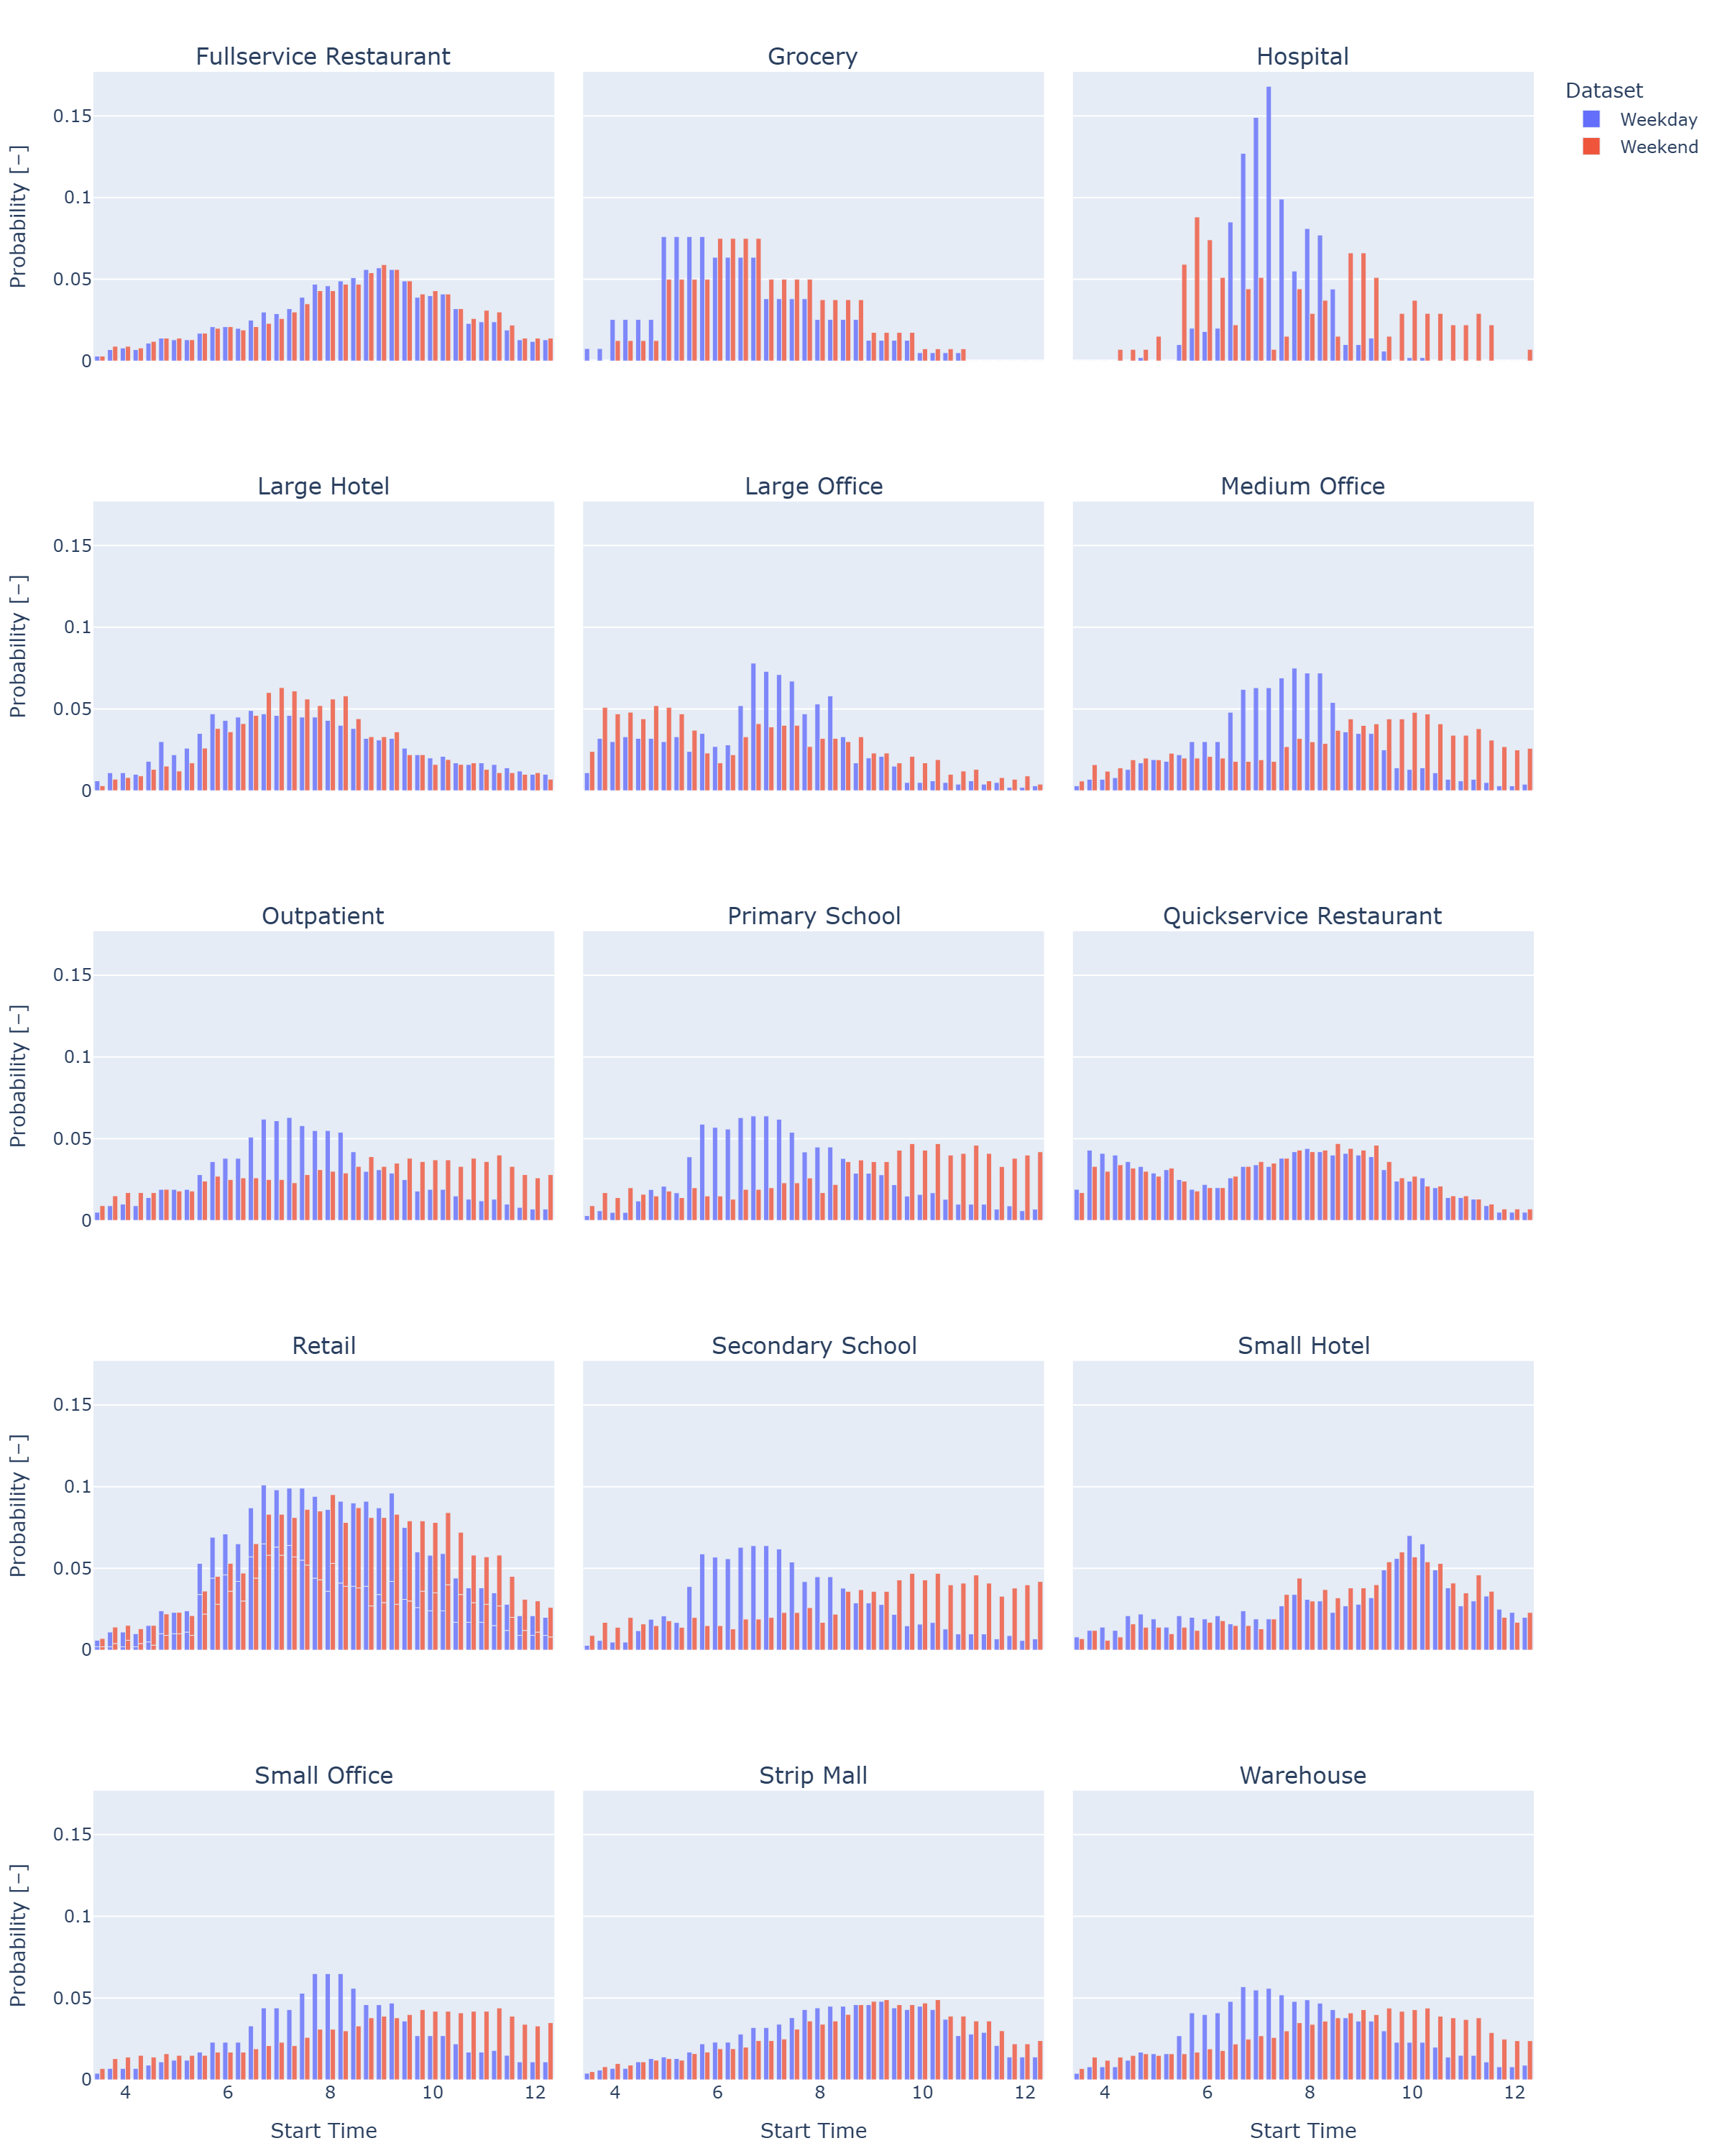
\includegraphics[width=1\textwidth]{figures/start_time.png}
   \caption{Operating hours' start time distributions.}
    \label{fig:start_time}
\end{figure}

\begin{figure}
    \centering 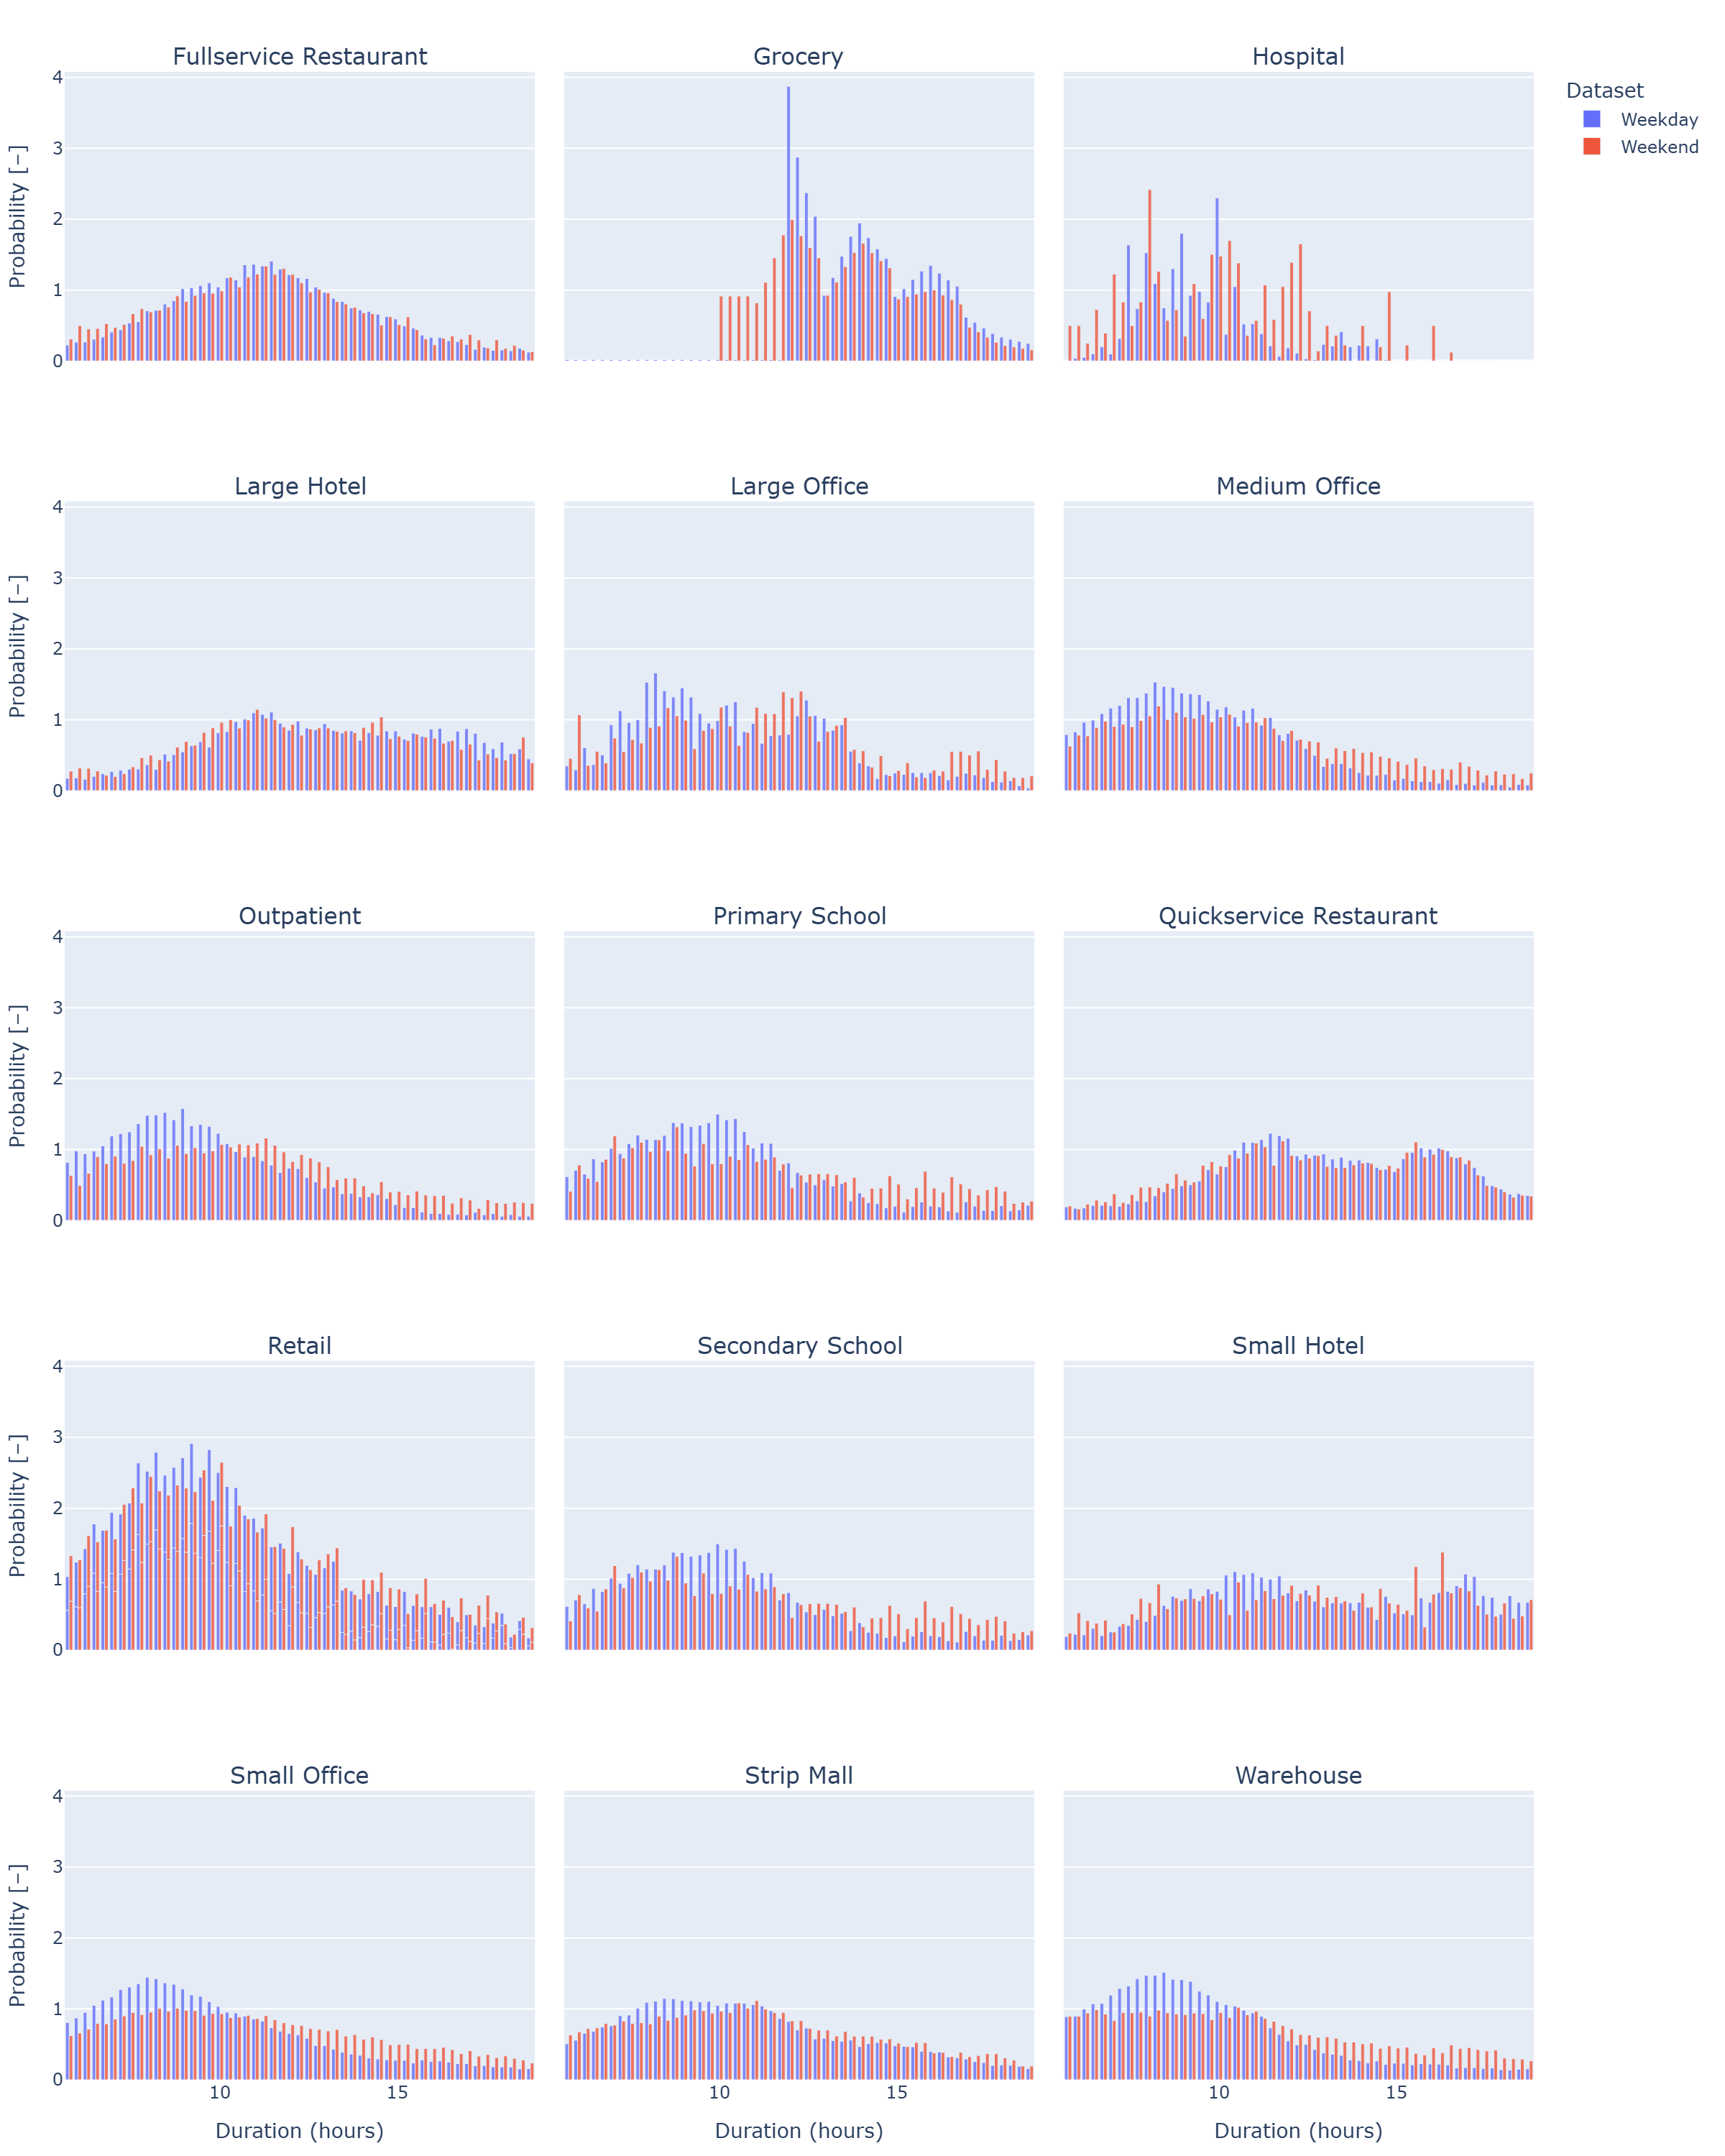
\includegraphics[width=1\textwidth]{figures/duration.png}
    \caption{Operating hours' duration distributions.}
    \label{fig:duration}
\end{figure}

\begin{figure}
    \centering 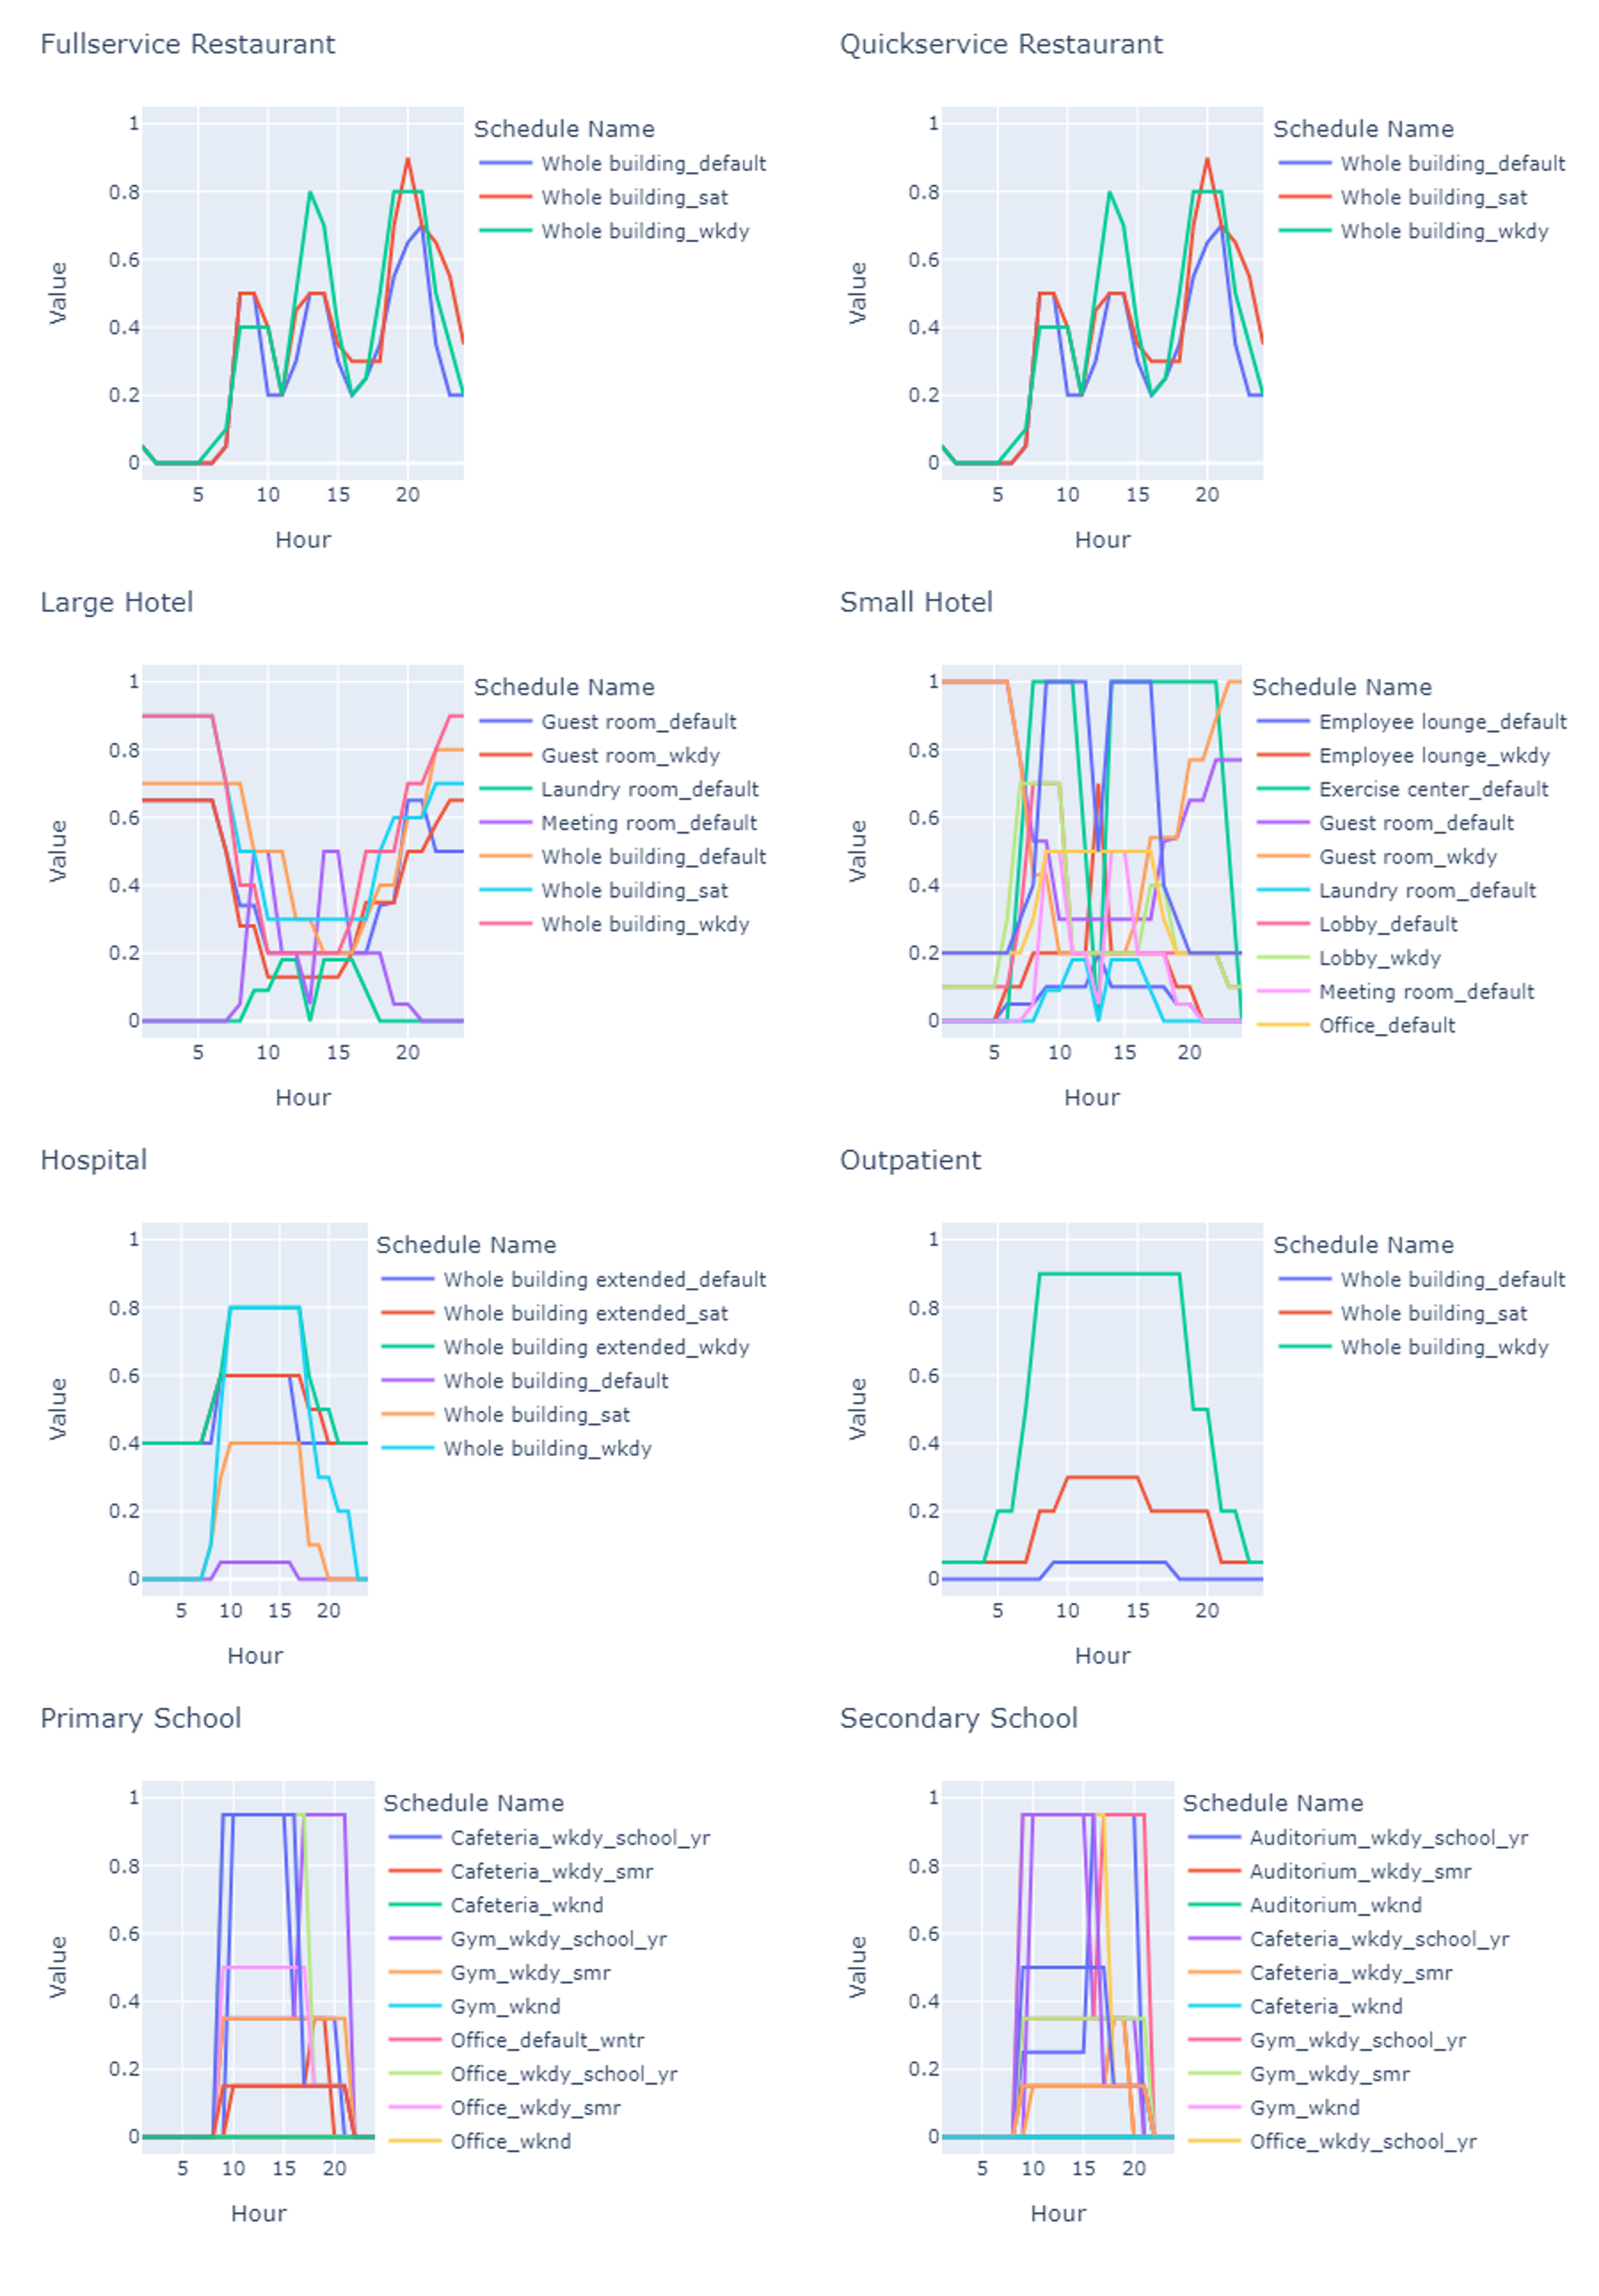
\includegraphics[trim={0 0 0 0}, clip,  % L B R T
    width=0.9\textwidth]{figures/occupancy_schedules_1.png}
    \caption[National base occupancy schedules excluding California]{National base occupancy schedules for food service, lodging, healthcare, and education ComStock building types, excluding California. See Figure \ref{fig:occupancy_schedules_deer_1} for California.}
    \label{fig:occupancy_schedules_1}
\end{figure} 

\begin{figure}
    \centering 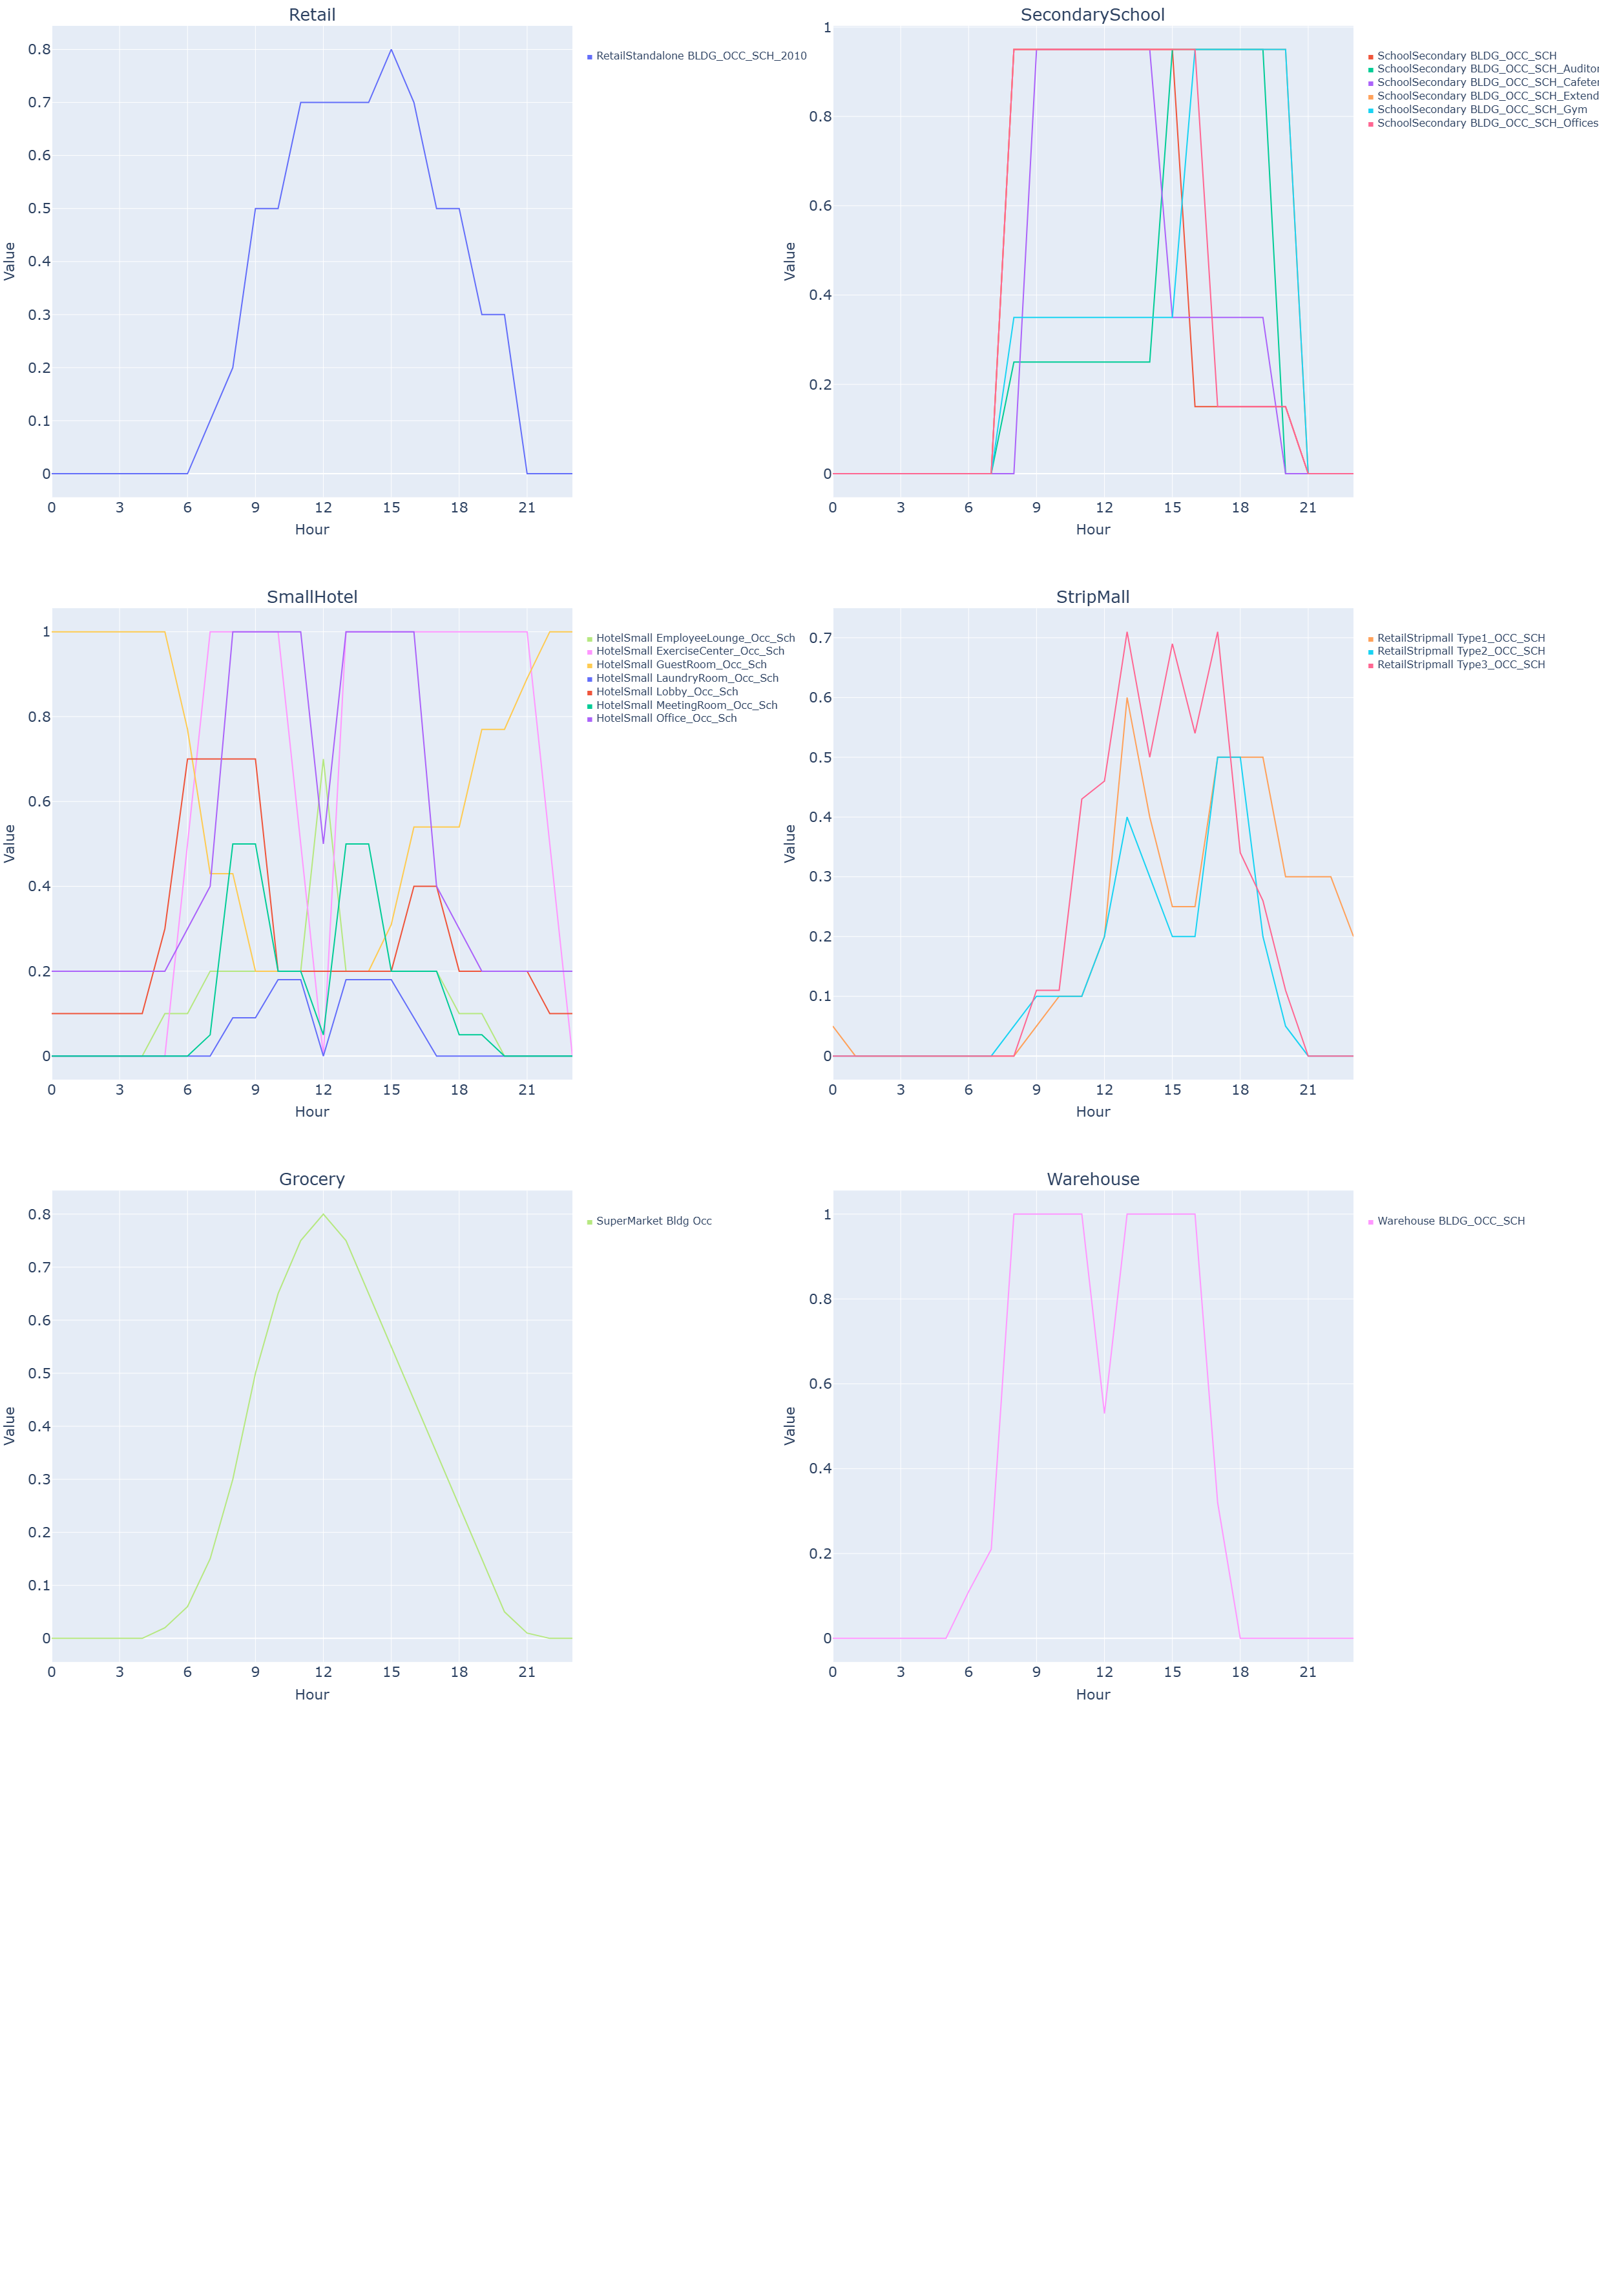
\includegraphics[trim={0 0 0 0}, clip,  % L B R T
    width=0.9\textwidth]{figures/occupancy_schedules_2.png}
    \caption[National base occupancy schedules excluding California]{National base occupancy schedules for retail, office, and warehouse ComStock building types, excluding California. See Figure \ref{fig:occupancy_schedules_deer_2} for California.}
    \label{fig:occupancy_schedules_2}
\end{figure} 
\section{Geometry}
\subsection{General}
A building's geometry influences several aspects of its associated building energy model. It impacts the building envelope by dictating the orientation of windows, the surface-to-volume ratio, and the ratio of one surface type to another. Geometry also impacts how prevalent solar heat gain is for a given building through the building's orientation and shape. ComStock uses seven characteristics to define a building energy model's geometry: floor area, shape, aspect ratio, rotation, number of floors, floor height, and window-to-wall ratio (WWR). The majority of these characteristics are assigned to the models as part of the sampling process. Combined, they create a virtual building model geometry like the example shown in Figure~\ref{fig:geom_example}. All building models are variations of rectangular prisms with flat roofs and windows wrapping around the exterior. This simple geometry allows ComStock to easily scale properties and generate the number of individual building models needed for a national stock model. The following subsections describe each of the seven characteristics that define a building energy model's geometry in ComStock.

\begin{figure}[h!]
    \centering 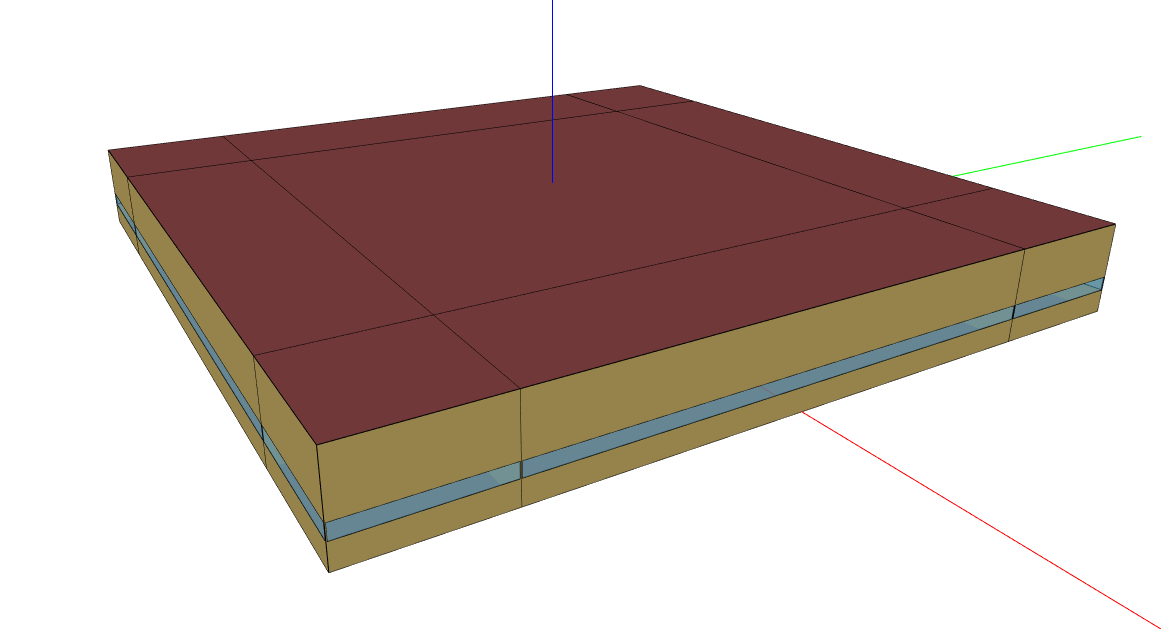
\includegraphics[width=0.7\textwidth]{figures/small_office_geometry.PNG}
    \caption[Example building geometry for a small office]{Example building geometry for a small office.}
    \label{fig:geom_example}
\end{figure}

\vspace{40mm} %blank space
\begin{center}
 (Intentionally blank)   
\end{center}


\pagebreak

\subsection{Area}
Building floor area is assigned to each model through the sampling process. Probability distributions were generated using CoStar \citep{costar} for most building types. HSIP \citep{hsip} was used for schools and hospitals, as neither are well represented in CoStar.

Figure~\ref{fig:area_dist} shows the breakdown of each building type in the national building stock by building size category (referred to as ``rentable area'').  Notice that the categories are presented as ranges.  At this time, ComStock uses the area in the middle of the range, with the exception of "\_1000" and "over\_1mil," which use 1000 square feet and 1 million square feet, respectively.  This method could be improved by adding variability to the building areas by selecting a variety of areas within the range.

\begin{figure}[H]
    \centering 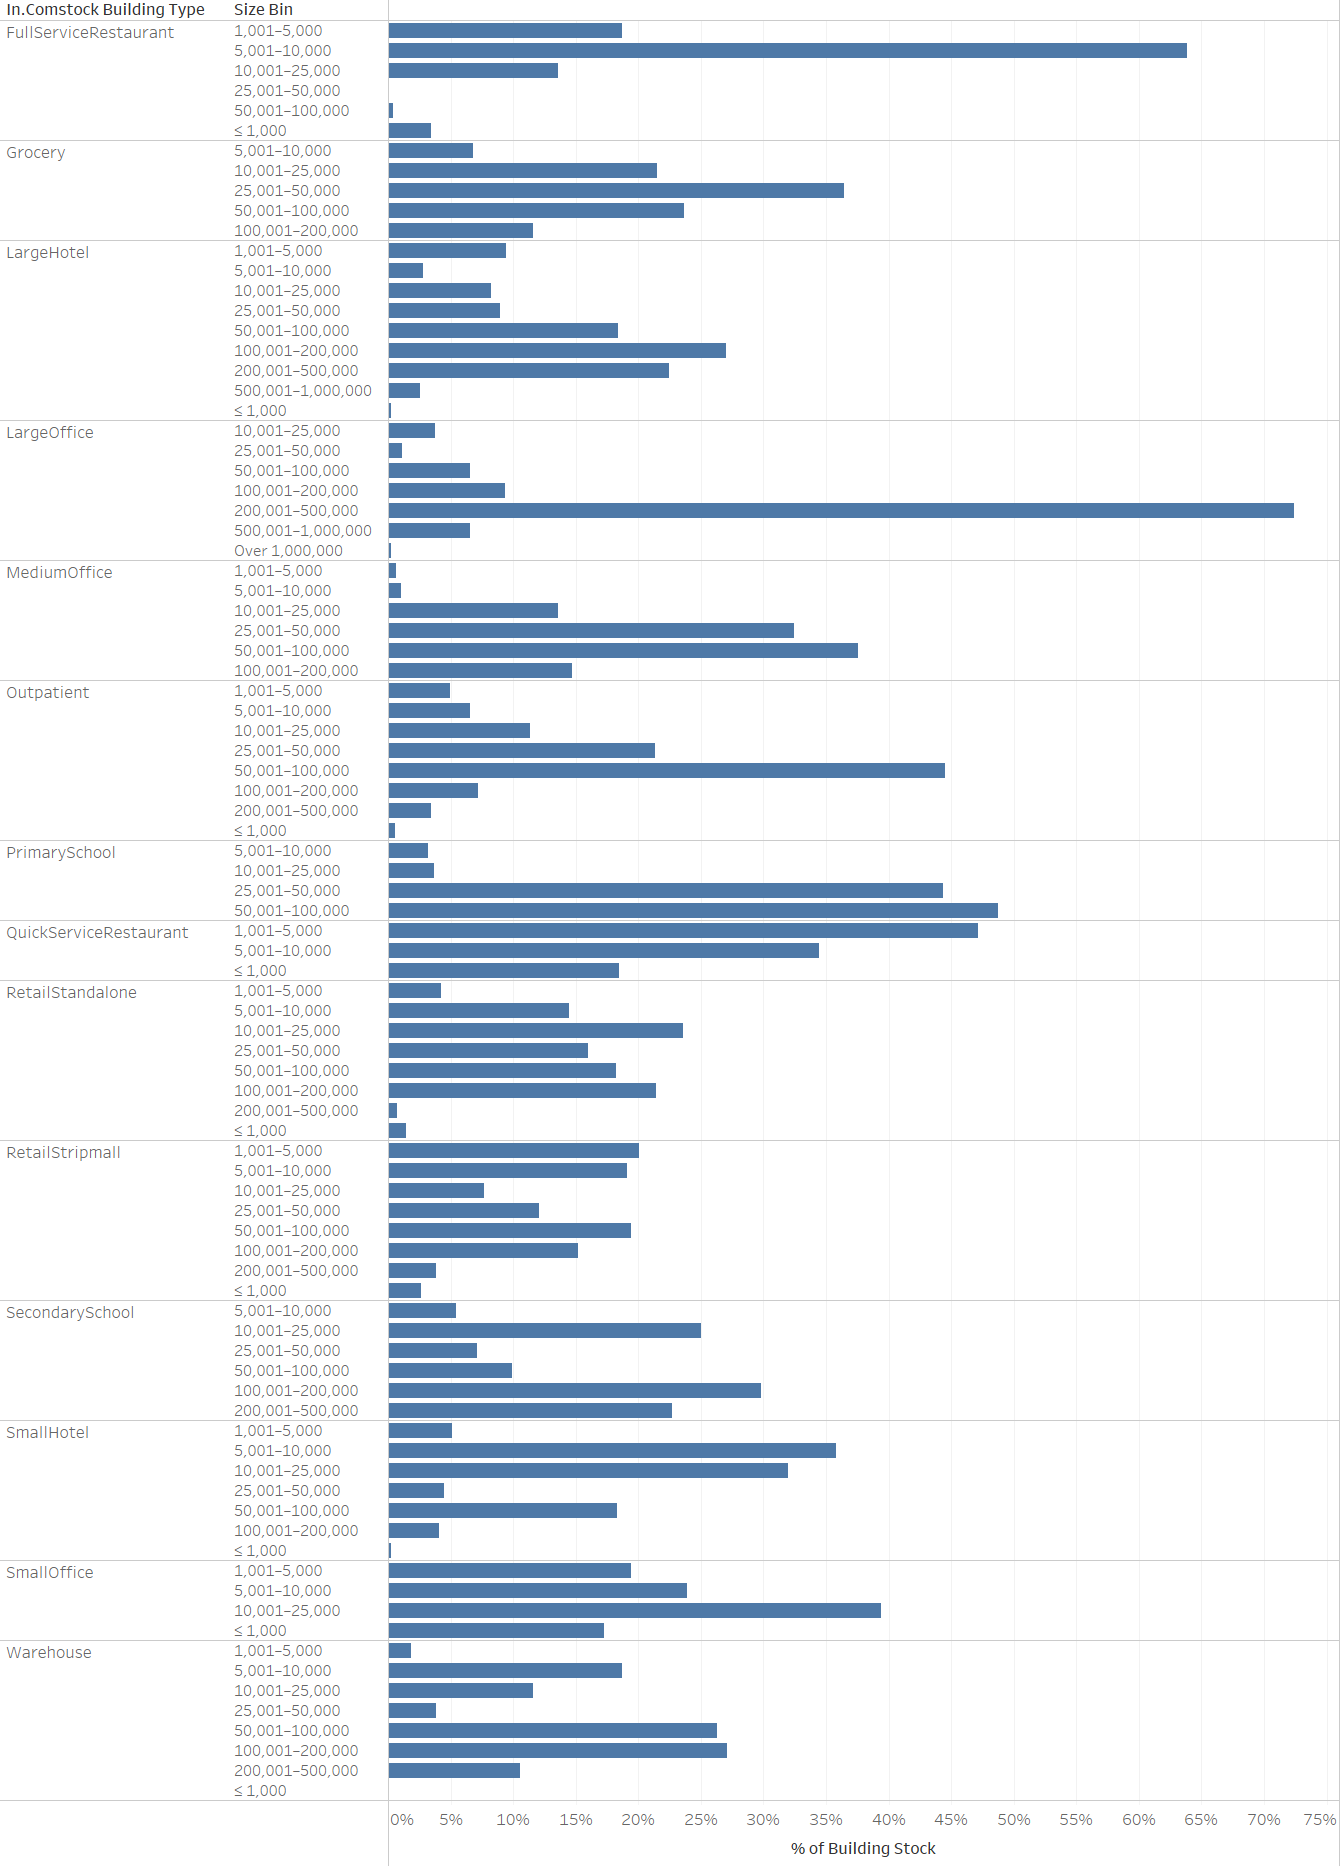
\includegraphics[width=1.0\textwidth]{figures/area_dist.png}
    \caption[Distribution of rentable area by building type]{Distribution of rentable area by building type. The x-axis represents rentable area (square feet), and the y-axis represents the fraction of the building stock.}
    \label{fig:area_dist}
\end{figure}

\pagebreak

\subsection{Building Shape}
Building shape is an intermediate characteristic assigned to the model during the sampling process. It is not a direct input to the model, as ComStock assumes a rectangular footprint for all buildings. Its function is as a dependency for aspect ratio (see next section \ref{subsec_aspect_ratio}). Probability distributions for building shape were generated from 2012 CBECS data, based on building type \citep{eia2012cbecs}. CBECS uses numbers to represent many of the answers to survey questions, and ComStock adopted these numbers to represent building shapes. 

Figure~\ref{fig:shape_dist} shows the breakdown of the national building stock by building shape and type. 

\begin{figure}[H]
    \centering 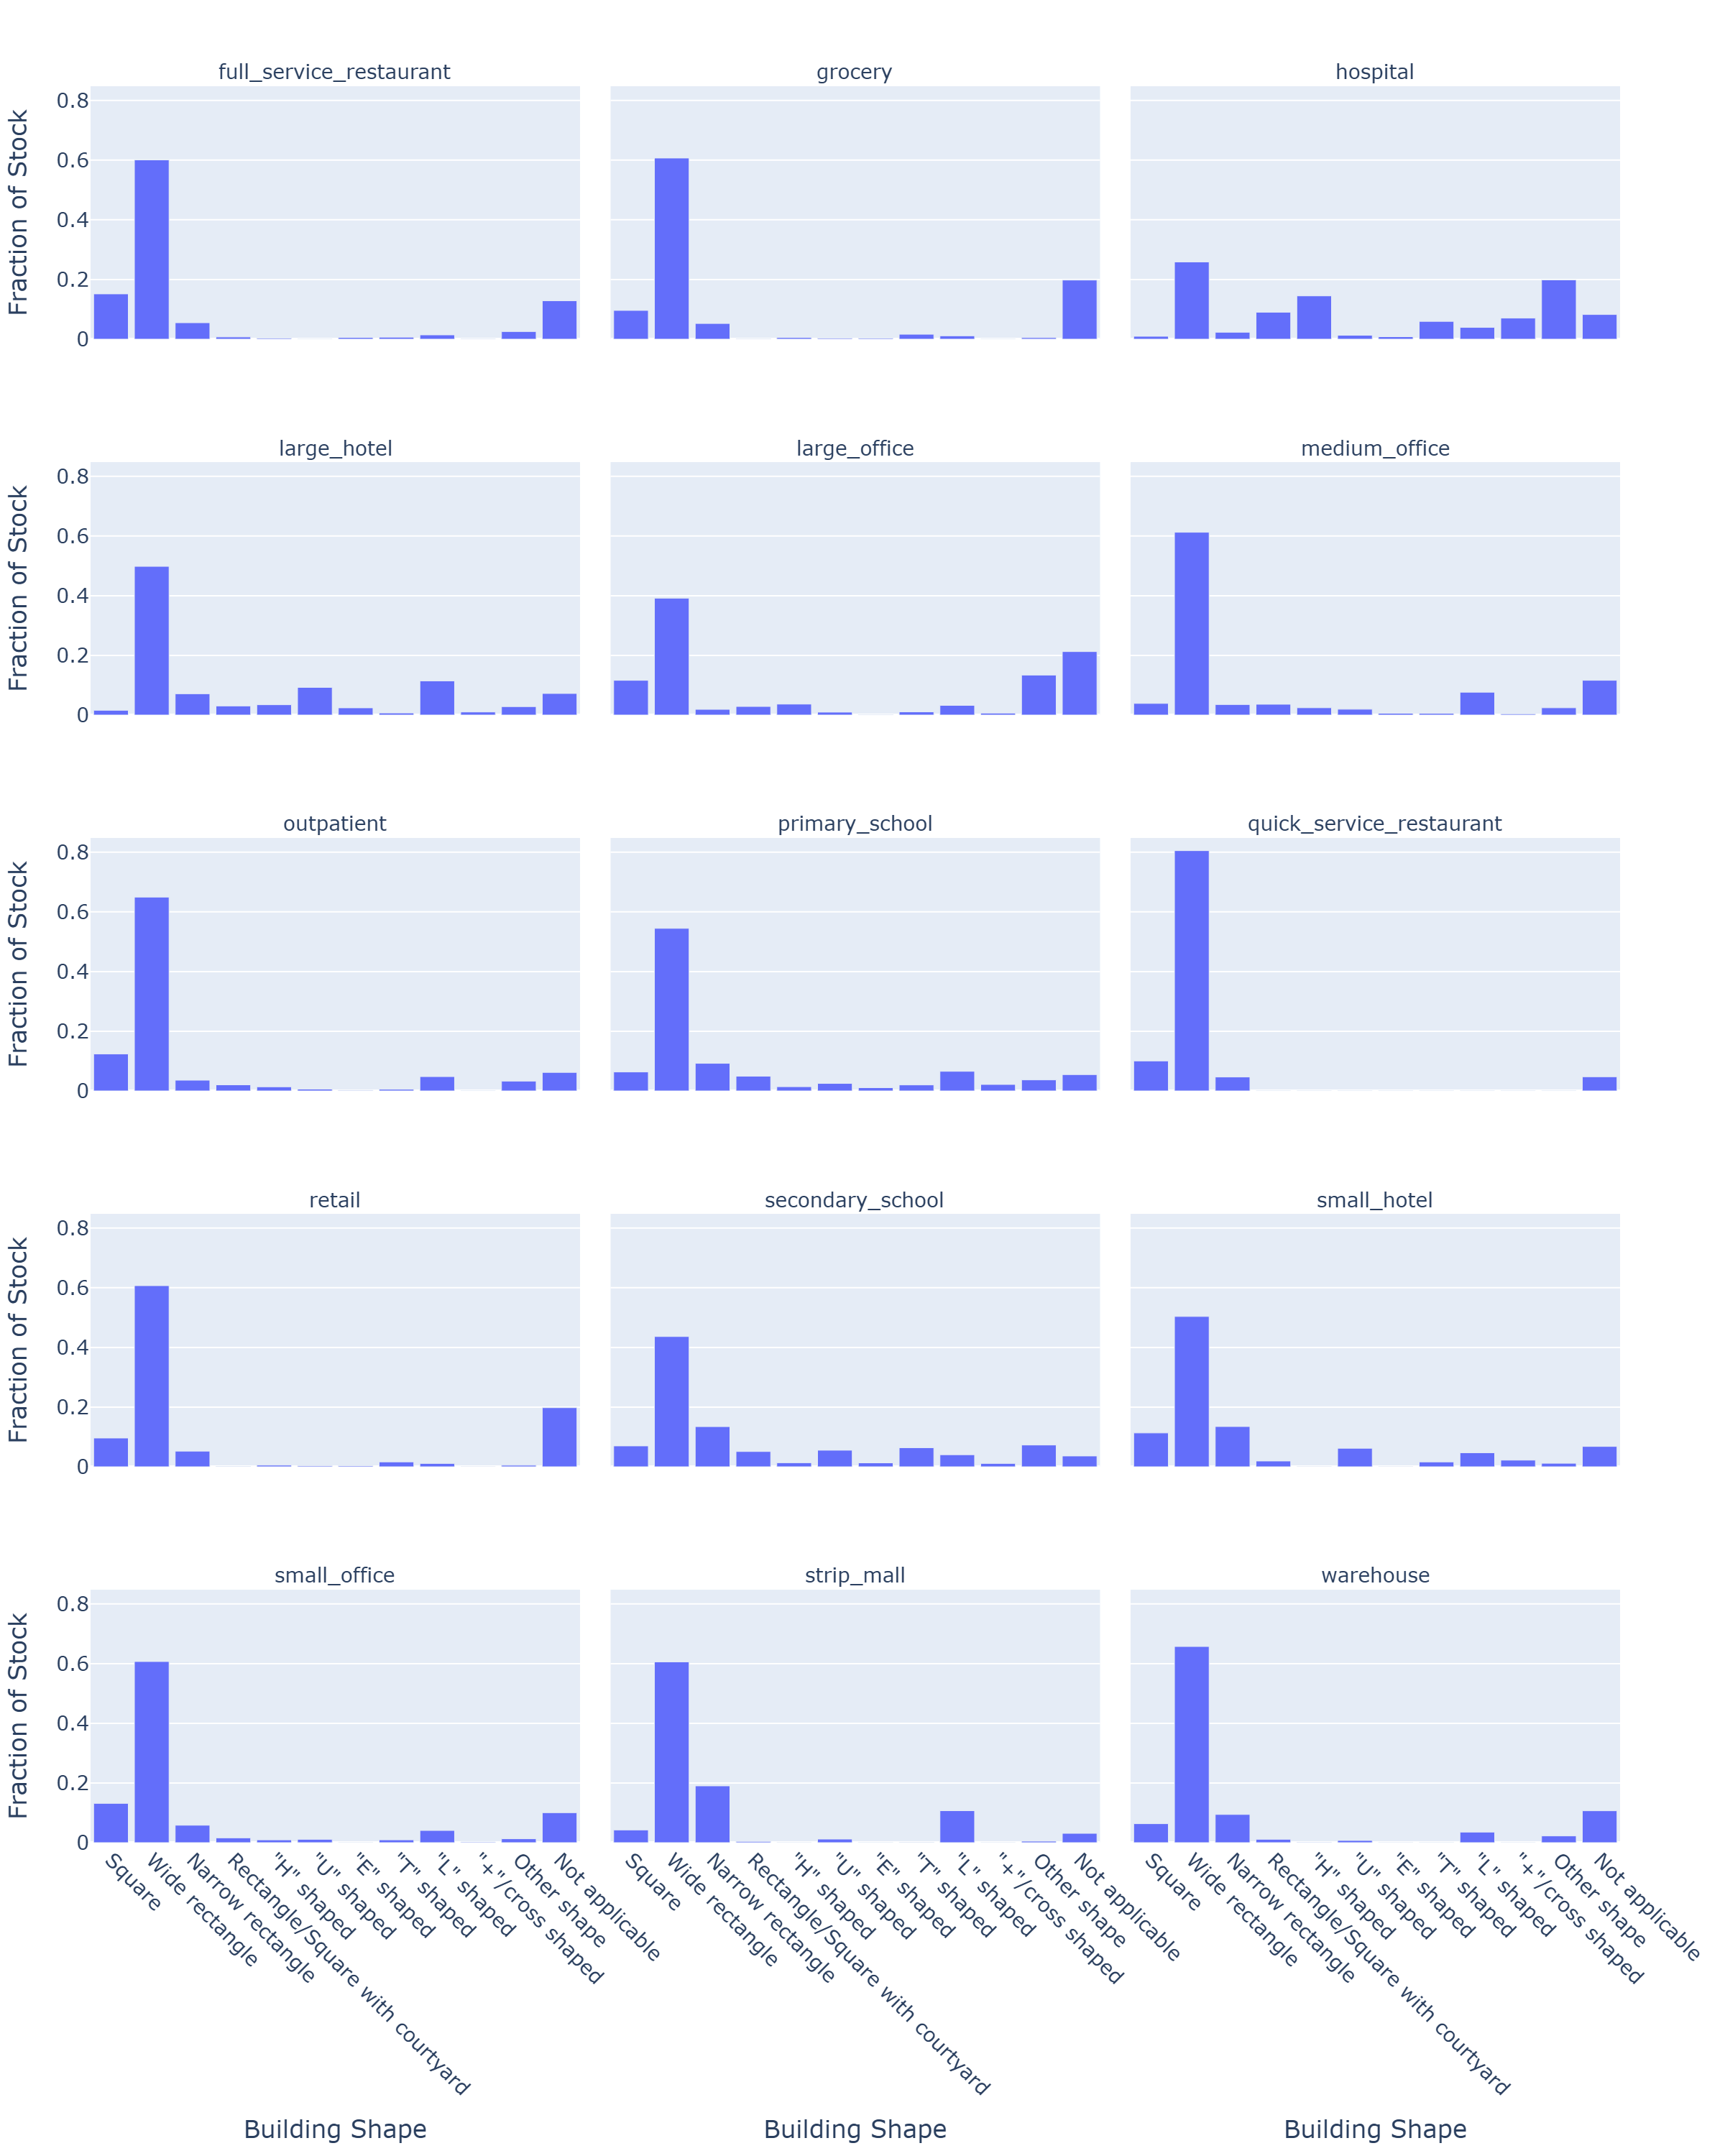
\includegraphics[width=1.0\textwidth]{figures/shape.png}
    \caption[Distribution of building shape by building type.]{Distribution of building shape by building type. The x-axis represents the building shape, and the y-axis represents the fraction of the building stock.}
    \label{fig:shape_dist}
\end{figure}

\pagebreak

\subsection{Aspect Ratio} \label{subsec_aspect_ratio}
Aspect ratio is defined as the overall length in the east–west direction divided by the overall length in the north–south direction. It is assigned to the building models during the sampling process. Probability distributions based on building shape were generated from 2012 CBECS data \citep{eia2012cbecs}.

Figure~\ref{fig:aspect_ratio_dist} shows the breakdown of the national building stock by aspect ratio. The aspect ratios are integers from one to six, which represent a building's north-south:east-west ratio.

\begin{figure}[H]
    \centering 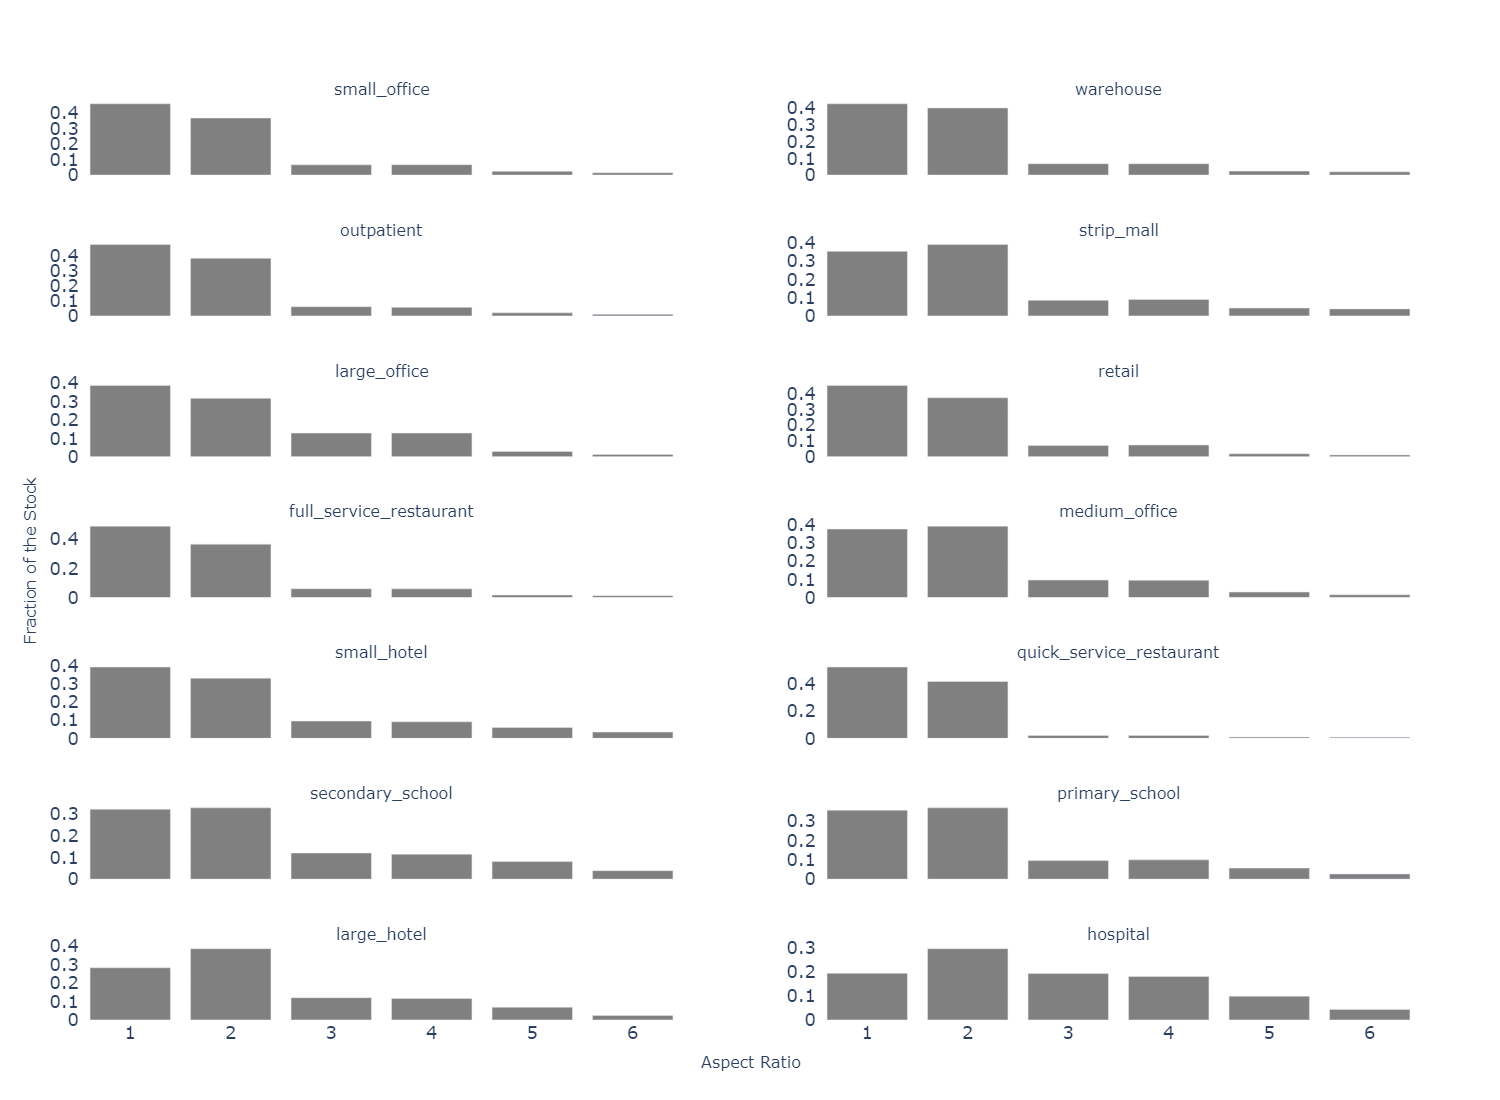
\includegraphics[width=1.0\textwidth]{figures/aspect_ratio.png}
    \caption[Distribution of aspect ratio by building type]{Distribution of aspect ratio by building type. The x-axis represents the aspect ratio (an integer from 1--6), and the y-axis represents the fraction of the building stock.}
    \label{fig:aspect_ratio_dist}
\end{figure}

\pagebreak

\subsection{Rotation}
Rotation defines the orientation of the building relative to the cardinal directions. In ComStock, there are eight rotation options, ranging from 0 to 315 degrees at 45-degree intervals. Ninety and 270 degrees correspond to a north-south length and east-west width (Figure~\ref{fig:rotation}). Rotations are evenly distributed throughout the building stock due to a lack of available data for more detailed distributions. This will be improved if new data becomes available.

\begin{figure}[H]
    \centering 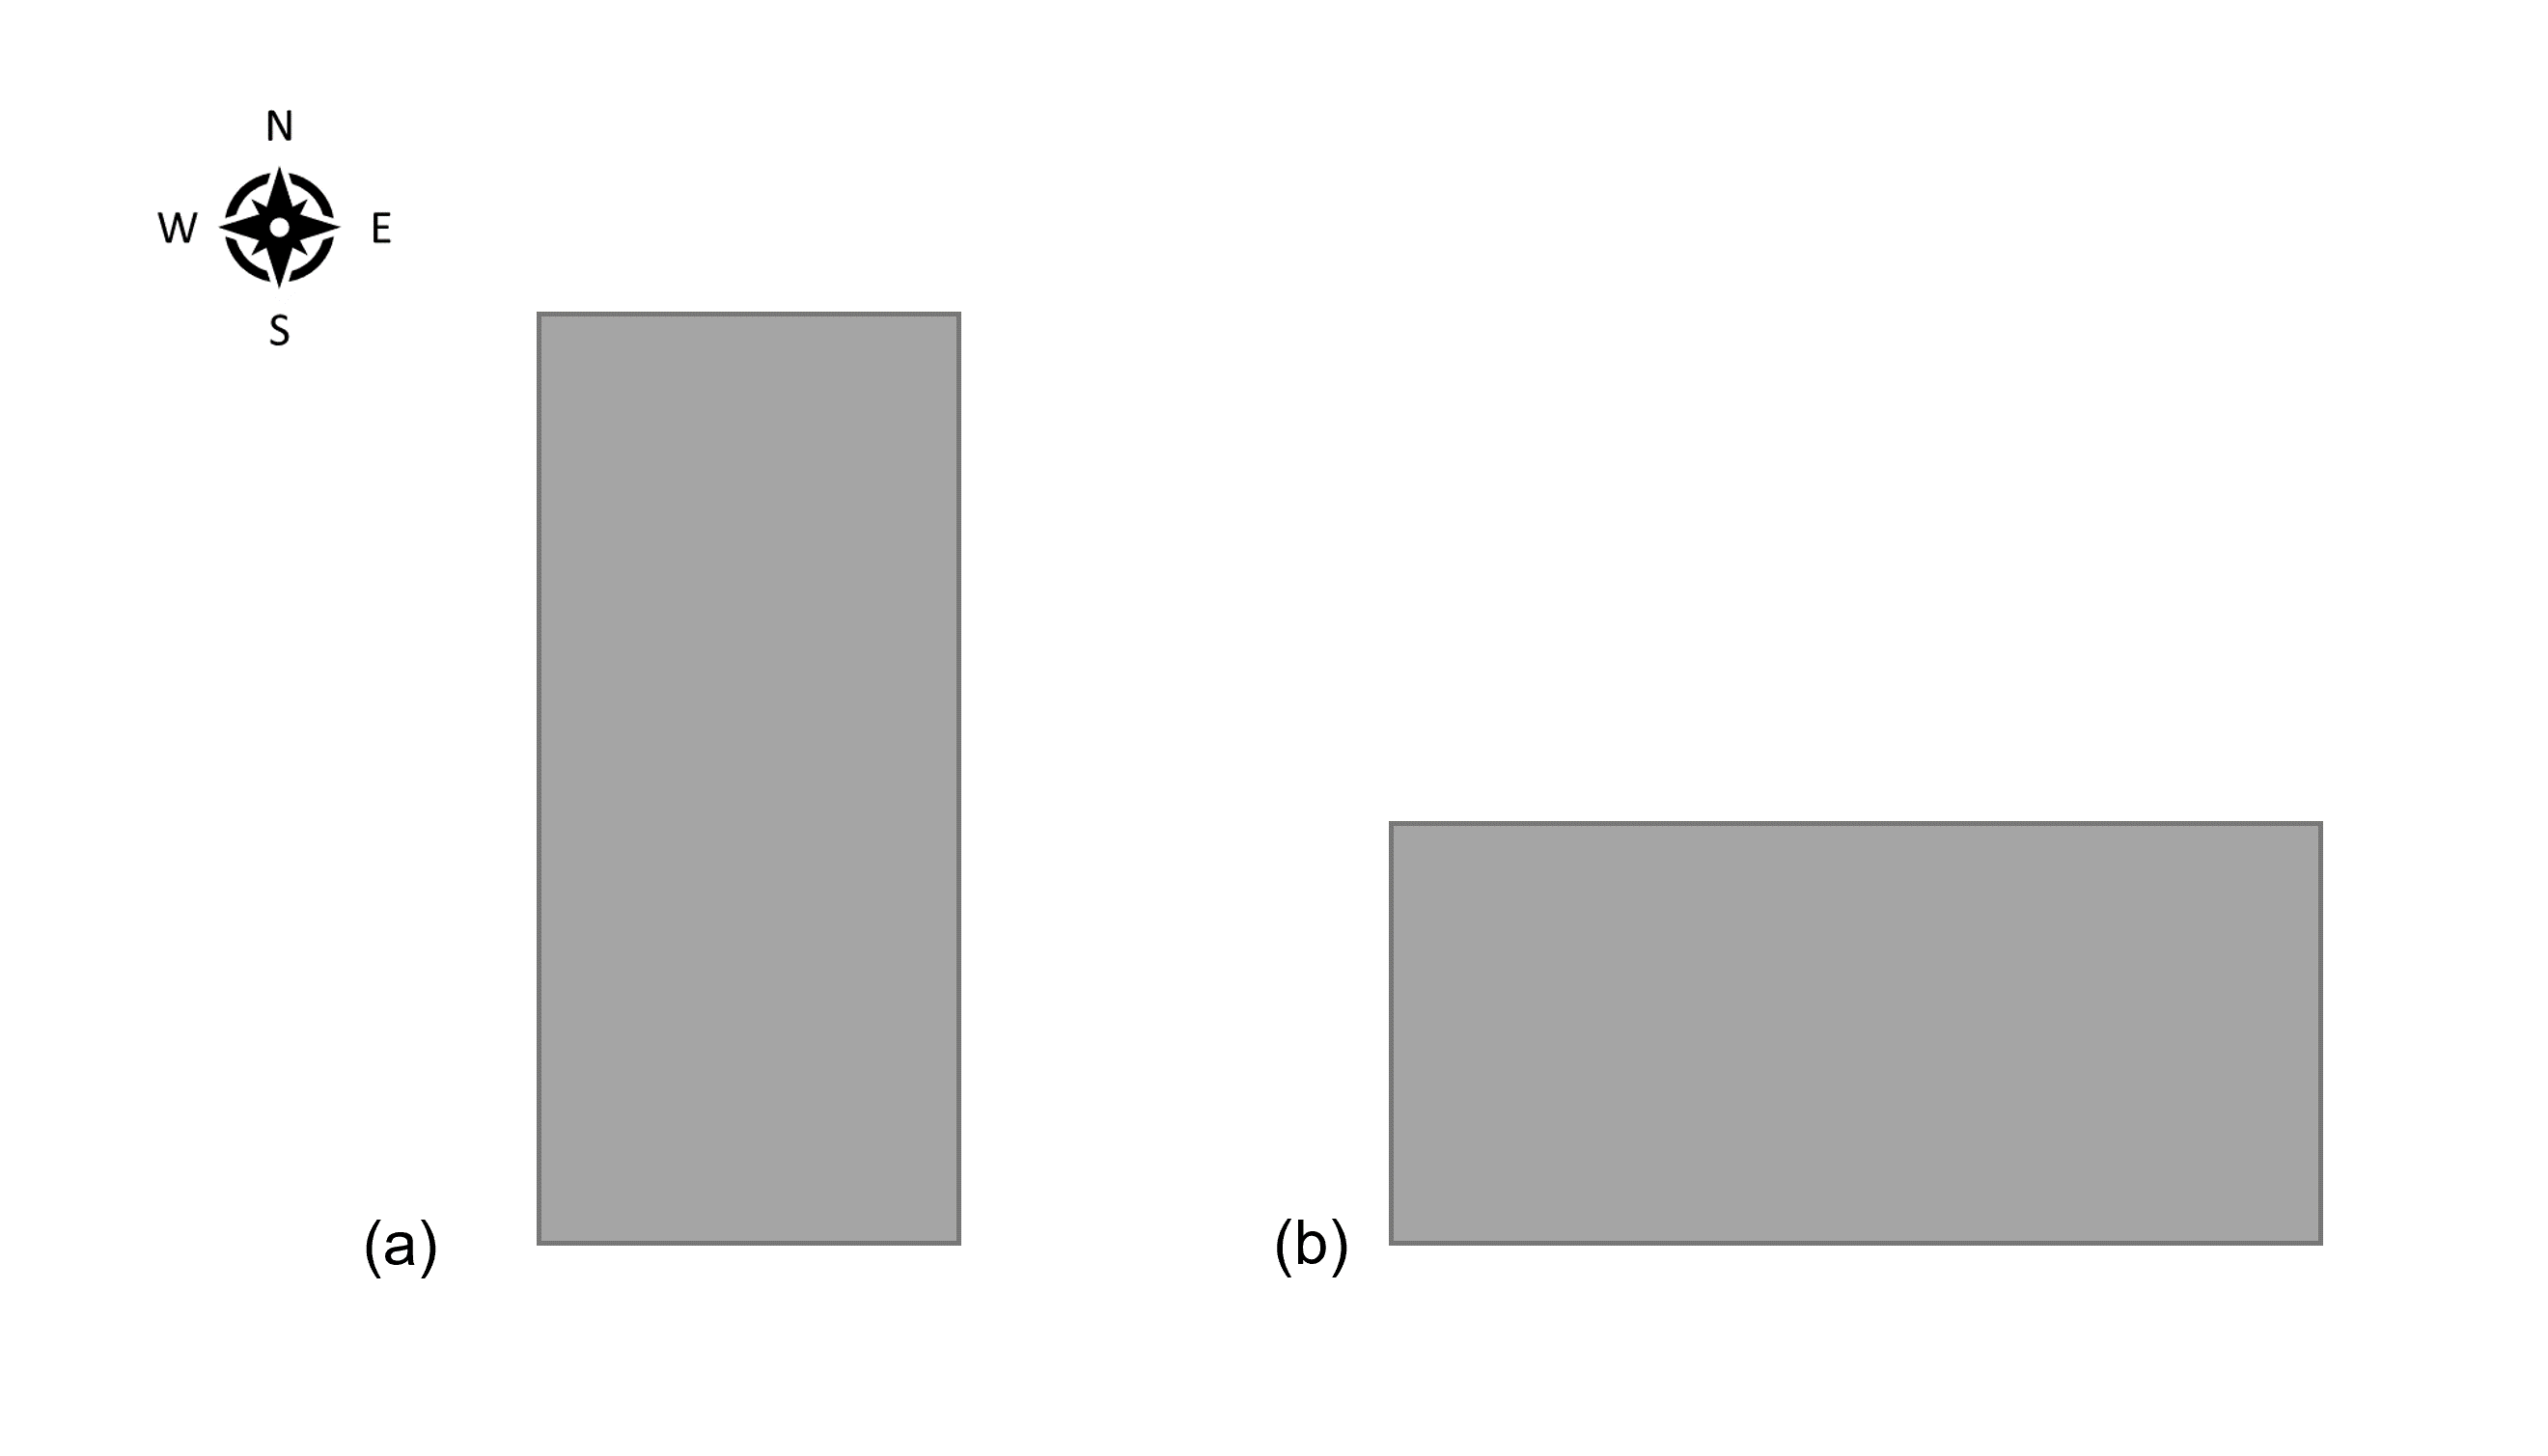
\includegraphics[width=0.7\textwidth]{figures/rotation_example.png}
    \caption[Building rotation]{Illustration of building rotation. (a) Buildings with either 90 or 270 degree rotation have a north-south length. (b) Buildings with either 0 or 180 degree rotation have an east-west length.}
    \label{fig:rotation}
\end{figure}

\subsection{Floor Height}
Floor height is represented in the models as floor-to-floor height. ComStock uses the floor-to-floor heights found in the DOE prototype buildings, which were established using expert opinion \citep{deru_2011}. These floor-to-floor heights are summarized in Table~\ref{tab:floor_height}.

\begin{table}[h]
\small
\centering
\caption[Floor-to-Floor Heights]{Floor-to-Floor Heights by Building Type}
\label{tab:floor_height}
\small
\begin{tabular}{|c|c|}
\hline
\textbf{Building Type}   & \textbf{Floor-to-Floor Height (feet)} \\ \hline
Full Service Restaurant  & 10                                    \\ \hline
Hospital                 & 14                                    \\ \hline
Large Hotel              & Ground: 13; Upper: 10                 \\ \hline
Large Office             & 13                                    \\ \hline
Medium Office            & 13                                    \\ \hline
Outpatient               & 10                                    \\ \hline
Primary School           & 13                                    \\ \hline
Quick Service Restaurant & 10                                    \\ \hline
Retail                   & 20                                    \\ \hline
Secondary School         & 13                                    \\ \hline
Small Hotel              & Ground: 11; Upper: 9                  \\ \hline
Small Office             & 10                                    \\ \hline
Strip Mall               & 17                                    \\ \hline
Warehouse                & 28                                    \\ \hline
\end{tabular}
\end{table}

\pagebreak

\subsection{Number of Floors}
ComStock assigns a number of floors to each model during the sampling process to create a distribution of building heights in the stock. This value represents the number of aboveground floors for a given model. No buildings in ComStock have belowground stories.

 For most of the building types, we generated probability distributions based on county and building type using CoStar \citep{costar}. We used HSIP \citep{hsip} for schools and hospitals, as neither are well-represented in CoStar.
 
 Figure~\ref{fig:nfloors_dist} shows the breakdown of the national building stock by number of floors and building type.

\begin{figure}[H]
    \centering 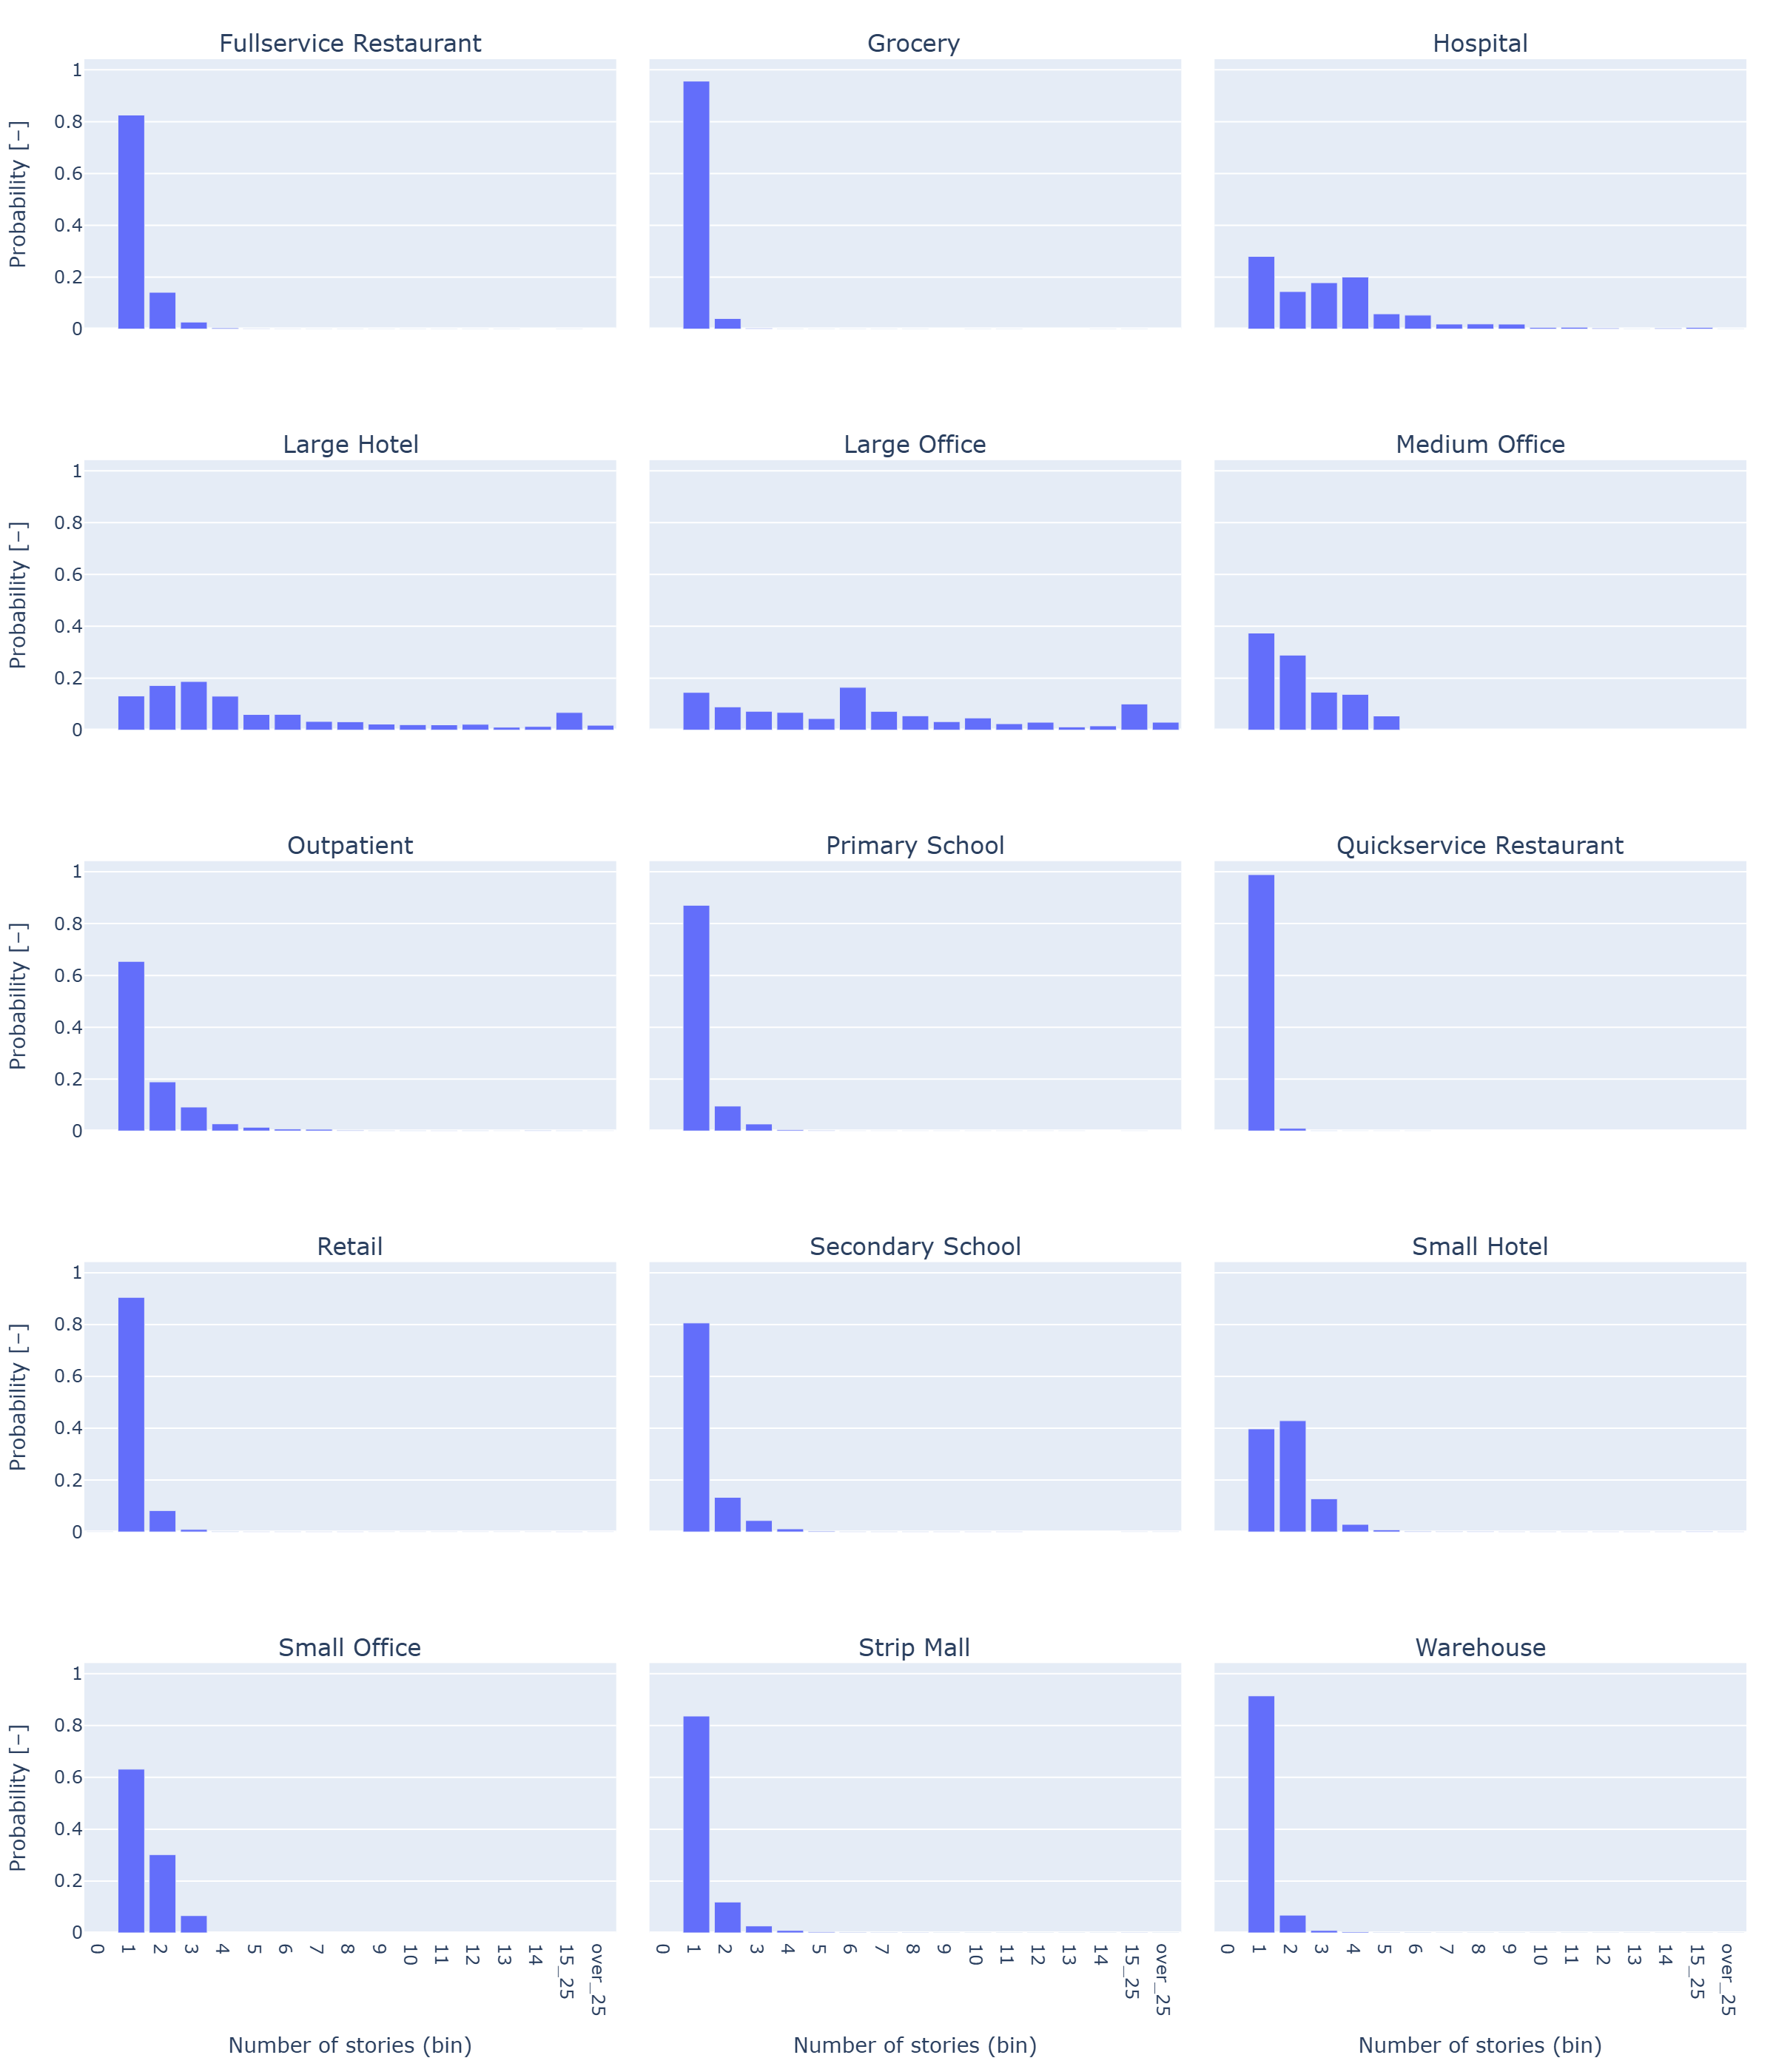
\includegraphics[width=1.0\textwidth]{figures/nfloors.png}
    \caption[Distribution of number of aboveground  floors by building type]{Distribution of number of aboveground  floors by building type. The x-axis represents the number of floors, and the y-axis represents the fraction of the building stock.}
    \label{fig:nfloors_dist}
\end{figure}

\pagebreak

\subsection{Window-to-Wall Ratio (WWR)}
The ComStock window-to-wall ratio (WWR) assumptions were created as part of the EULP project. WWR is defined as the fraction of abovegrade wall area that is covered by fenestration. Previously, ComStock used the WWR from the DOE prototype building models. Although each building type had a different WWR, there was no variability within each building type, which is not representative of the building stock. To address this issue, we referenced the NFRC Commercial Fenestration Market Study conducted by Guidehouse \citep{guidehouse_nfrc_window_report}. The study characterized the national commercial window stock through data collection and analysis. Six primary data sources representing all regions of the United States were used in the study---a 2020 Guidehouse survey, NEEA CBSA, DOE Code Study, CAEUS, CBECS, and RECS (multifamily). A variety of window properties were collected, including WWR, number of panes, frame material, glazing type, low-emissivity coating, gas fill, and many others. In total, the database contained approximately 16,000 samples, each with an appropriate weighting factor based on the coverage, completeness, and fidelity of each data source. We incorporated the WWR results from this study into the ComStock model, and we may incorporate other fields in the future to further refine our window modeling methodology.

From the Guidehouse data, we developed a WWR distribution for each combination of building type, floor area, and vintage. We first analyzed the WWRs separately by building type, floor area, geographic location, and vintage to determine which filters were appropriate to use for the final distributions. Geographic location did not have a significant impact on WWR, so it was left out of the final distributions. As can be seen in Figures~\ref{fig:wwr_by_rentable_area} and~\ref{fig:wwr_by_building_vintage}, there is a noticeable change in the WWR of buildings built after 2014, indicating that new buildings are trending toward larger windows. Similarly, there is a distinct trend in the WWR as a function of floor area; larger buildings tend to have more windows. Whereas the previous methodology only varied WWR by building type, these new distributions introduce more WWR variability by considering vintage and floor area.

The WWR distributions for all buildings before and after incorporating the NFRC data are shown in Figure \ref{fig:wwr_before_after_all_buildings}. The distinct bins in the graph are a result of the way WWR is binned in the CBECS Show Card: 0\%--1\% WWR is binned to 0.0, 2\%--10\% to 0.06, 11\%--25\% to 0.18, 26\%--50\% to 0.38, 51\%--75\% to 0.63, and 76\%--100\% to 0.88. The final distributions do not change the stock total energy consumption significantly, but they do add realistic variability within building types. For example, previously, all large offices had the same WWR of 0.15, whereas using the new distributions, large office WWRs vary from 0.01 to 0.88.

    \begin{figure} [h]
    \centering 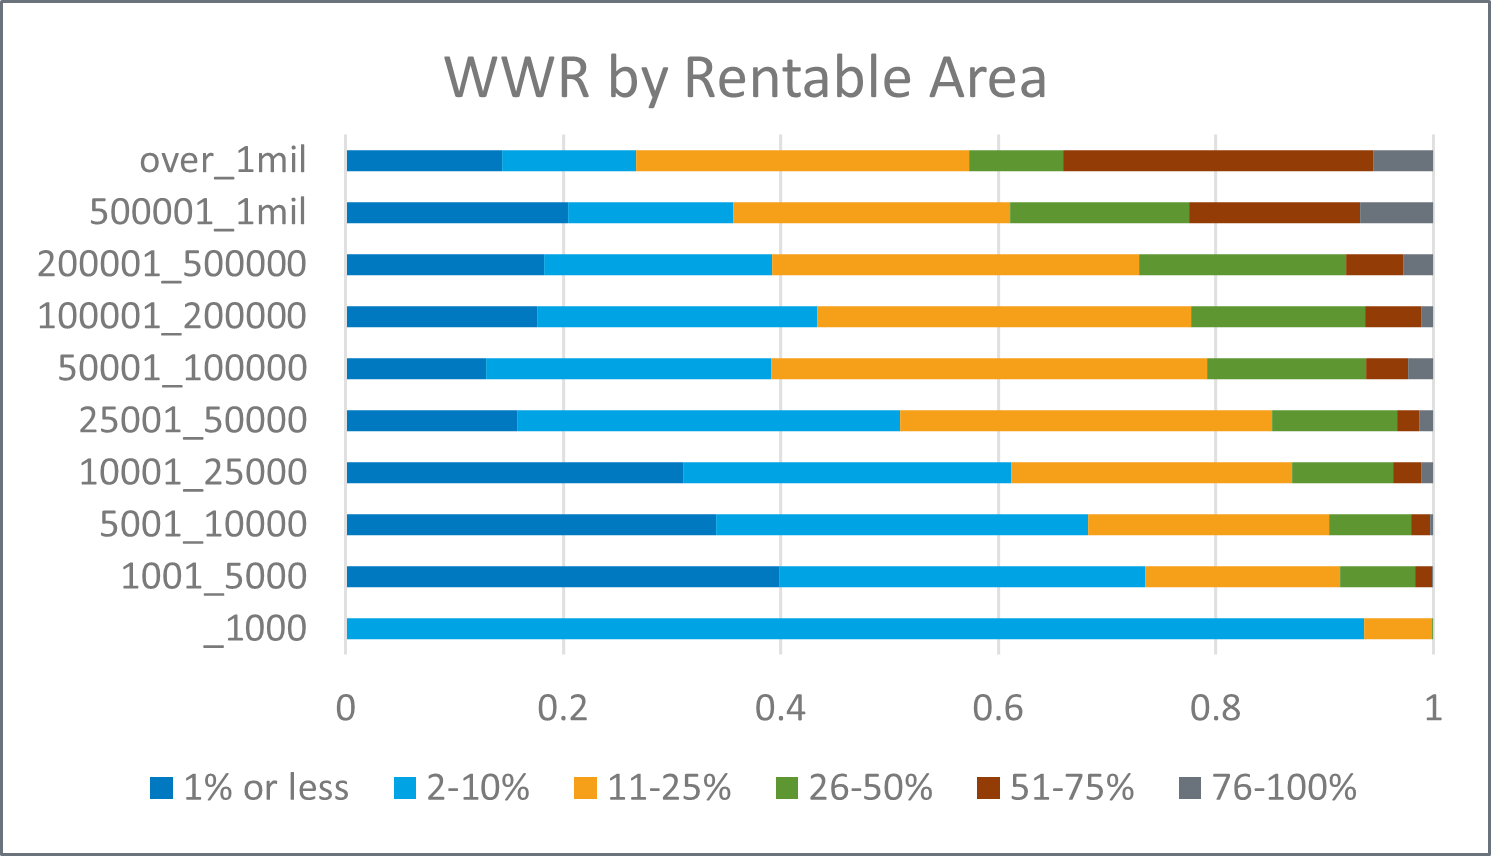
\includegraphics[width=\textwidth]{figures/wwr_by_rentable_area.png}
    \caption[Window-to-wall ratio by rentable floor area]{Window-to-wall ratio by rentable floor area.}
    \label{fig:wwr_by_rentable_area}
    \end{figure} 

\pagebreak

    \begin{figure} [h]
    \centering 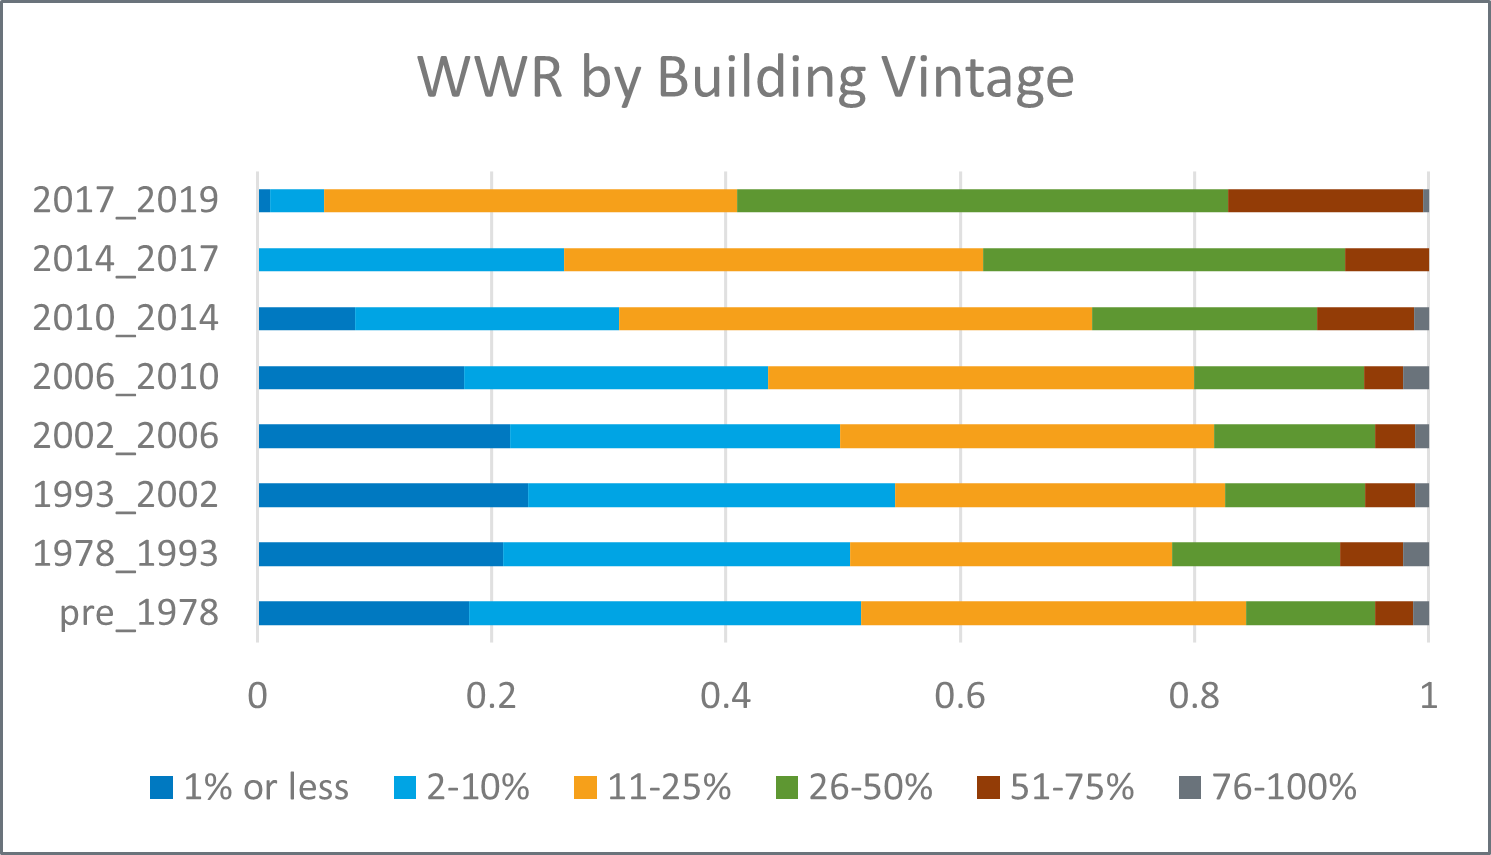
\includegraphics[width=\textwidth]{figures/wwr_by_building_vintage.png}
    \caption[Window-to-wall ratio by building vintage]{Window-to-wall ratio by building vintage.}
    \label{fig:wwr_by_building_vintage}
    \end{figure} 

    \begin{figure}[h!]
    \centering 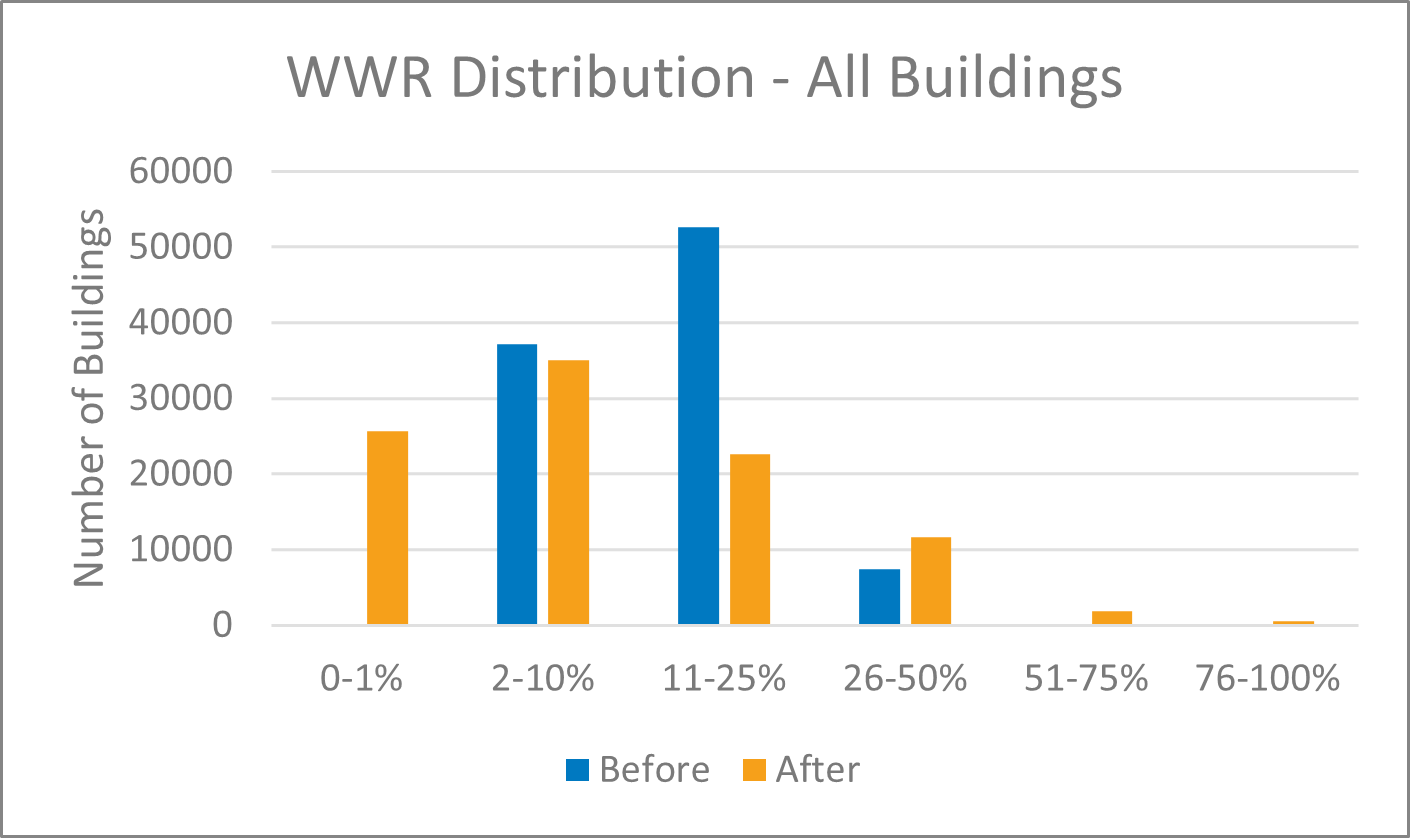
\includegraphics[width=\textwidth]{figures/wwr_before_after_all_buildings.png}
    \caption[Window-to-wall ratio distribution]{Window-to-wall ratio distribution in all building types before and after incorporating NFRC data.}
    \label{fig:wwr_before_after_all_buildings}
    \end{figure} 

\pagebreak

\subsection{Space Programming and Thermal Zoning}
As described above, all ComStock building models are a rectangular prism with a prescribed aspect ratio, floor area, etc. Within each building, there are one or more space types, as described in Section \ref{sec:space_type_ratios}. Space types are represented within the rectangular geometry as ``slices'' through the building that correspond to the floor area fractions of each space type. This is shown in Figure \ref{fig:geometry_by_space_type_and_zone}(a). In the cases of very small buildings, this can sometimes result in spaces which are unrealistically long and narrow for space types that make up only a small fraction of the building.

For larger buildings where the length and width are both greater than 37.5 feet, each space type is divided into core-and-perimeter thermal zones with a 15-foot depth (Figure \ref{fig:geometry_by_space_type_and_zone}(b)). Notice that the space types adjacent to the shorter ends of the building are each broken into six thermal zones, whereas the space types in the center of the building are each broken into three thermal zones. In multistory buildings, space types are often found on more than one floor, and in some cases, a floor will be a single space type. The downside to this thermal zoning approach is that thermal zones---and, as a follow-on, the HVAC systems that serve them---may be unrealistically small or large for certain geometry and building type combinations. These may later be modified to set a minimum and maximum size threshold for thermal zones.

\begin{figure}[hb!]
\centering 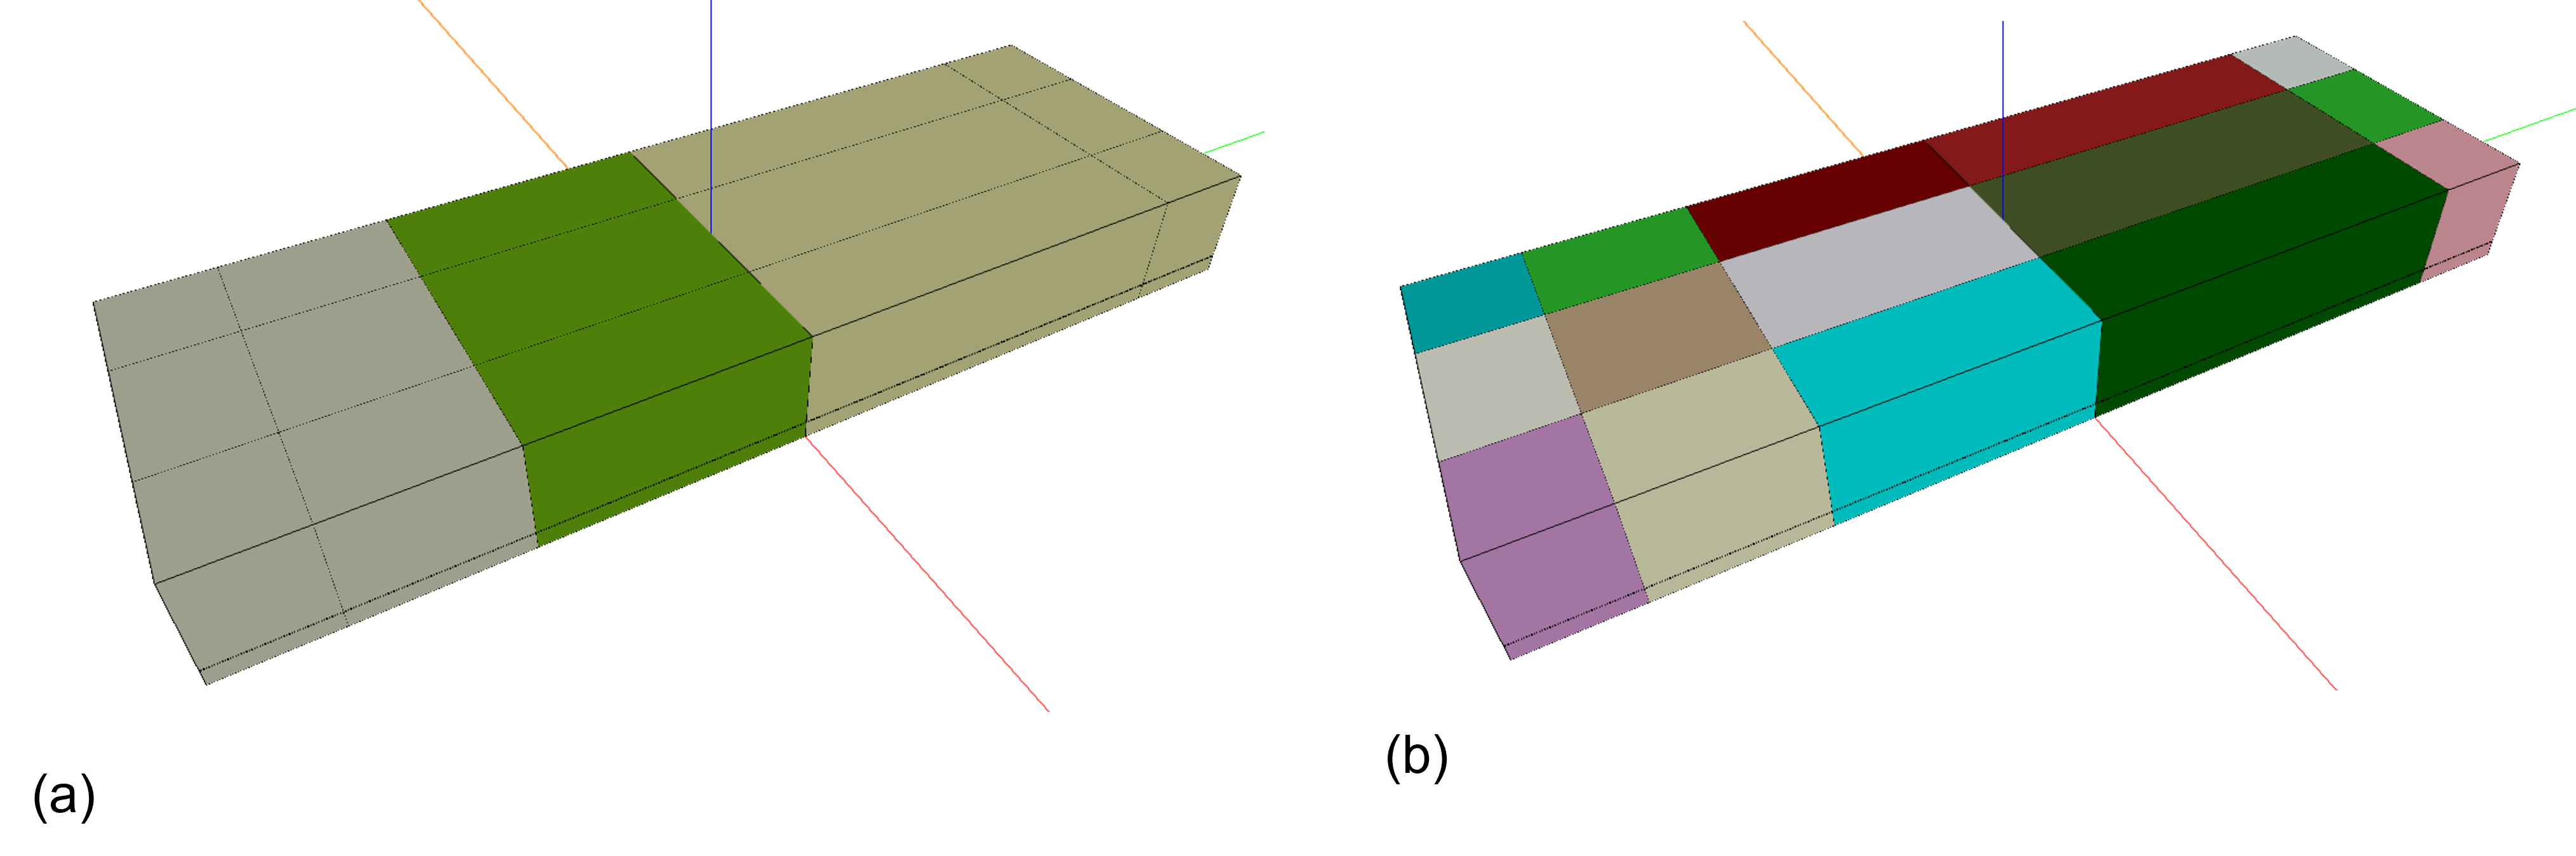
\includegraphics[width=1\textwidth]{figures/geometry_by_space_type_and_zone.png}
\caption[Example building geometry]{Example building geometry colored by (a) space type and (b) zone.}
\label{fig:geometry_by_space_type_and_zone}
\end{figure} 
\section{Envelope}
\subsection{Walls} % Andrew
\paragraph{Wall Construction Type}
First, we selected the general types of wall construction methods to be represented in ComStock. We chose the four general wall types commonly used in commercial building energy codes because they cover the most common wall construction types and can be linked to nominal thermal characteristics. The definitions of these types from \cite{ashrae_901_2010} are as follows, with the corresponding ComStock enumerations shown in parentheses:

\begin{itemize}
\item \textbf{Mass wall} (Mass): A wall with a heat capacity exceeding (1) 7 Btu/ft\textsuperscript{2}·F or (2) 5 Btu/ft\textsuperscript{2}·F, provided that the wall has a material unit weight not greater than 120 lb/ft\textsuperscript{3}.
\item \textbf{Metal building wall} (Metal Building): A wall whose structure consists of metal spanning members supported by steel structural members (i.e., does not include spandrel glass or metal panels in curtain wall systems).
\item \textbf{Steel-framed wall} (SteelFramed): A wall with a cavity (insulated or otherwise) whose exterior surfaces are separated by steel  framing members (i.e., typical steel stud walls and curtain wall systems).
\item \textbf{Wood-framed and other walls} (WoodFramed): All other wall types, including wood stud walls.
\end{itemize}

To determine the prevalence of each wall construction type, we queried a database, \cite{lightbox_smartparcels_2021}, containing  building type, number of stories, location, and wall construction. The database did not use the same wall construction types selected for ComStock, so we created a mapping between the database entries and the wall construction types listed above, as shown in Table~\ref{tab:wall_construction_mapping}. Some construction types in the database were excluded from the mapping, either because the meaning was ambiguous or because they represented an insignificant fraction of the entries in the database. The excluded constructions represent only 5\% of the total samples, with 4.5\% labeled “OTHER” (which there was no clear way to map).

Upon reviewing the data, we identified two instances that were likely misclassifications. The first was buildings higher than five stories with the wall construction type``WoodFramed''. Historically, it was not possible to use WoodFramed construction for buildings over five stories, and even today, this practice is uncommon. Buildings with this combination were reassigned to ``Mass'' walls, based on the assumption that people were observing large wood internal structural members in old buildings and classifying them as WoodFramed. The second was buildings higher than two stories with ``MetalBuilding'' walls. Based on experience, this construction technique is commonly reserved for 1--2 story buildings only. Buildings with this combination were reassigned to ``SteelFramed,'' based on the assumption that this would be the most likely alternative classification if a person observed steel structural elements.

After mapping each entry in the database to one of the ComStock construction types, we analyzed the data to determine other building characteristics in the database were correlated with construction type. Older buildings were slightly more likely to use mass constructions, but the change over time was minor. Construction type varied significantly as a function of the number of stories. Shorter buildings were much more likely to be wood-framed, whereas taller buildings were more likely to be mass, and very tall buildings were likely to be steel-framed (steel studs or curtain wall). Based on a spot-checking of the database, we found the building type classification to be less reliable than other building characteristics. Although there was some correlation between building type and wall construction, there was also a correlation between building type and number of stories. Because of the joint correlation, we selected number of stories instead of building type. There was a clear correlation between climate zone and construction type---most notably, there was a much lower incidence of mass walls in cold climate zones. There was some correlation between construction type and building floor area. However, there was also a correlation between the number of stories and the building area. Because the construction type is physically limited by a building's height, it was more logical to use the number of stories as a driving characteristic for construction type. Following this analysis, we concluded that the number of stories and climate zone should be used as drivers of wall construction type. The probabilities for each combination of number of stories and climate zone were calculated  and then used as the input distribution for wall construction type in ComStock. This distribution is summarized in Table~\ref{tab:wall_constuction_types}.

\paragraph{Wall System Turnover Rate}
As described in Section~\ref{sec:system_turnover_and_eul}, we assume that some building systems, including exterior walls, are replaced over the lifespan of the building. Typically, for exterior walls, the structural elements of the wall are maintained, while the cladding, insulation, sheathing, etc. are be replaced. As noted in Section~\ref{sec:system_turnover_and_eul}, the EUL for exterior walls is assumed to be 200 years, which means that most buildings are modeled with the walls they were built with. Once the wall construction type probabilities and distributions of building types, sizes, and vintages are carried through the sampling process and simulations are created, the distribution of construction types and energy code levels can be reviewed. As shown in Figure~\ref{fig:weighted_floor_area_by_energy_code_and_wall_type}, because the majority of the building stock is older, and wall systems are replaced at a low rate, most of the building floor area is assumed to have walls that follow the oldest energy codes.

\begin{figure}[ht!] \centering
    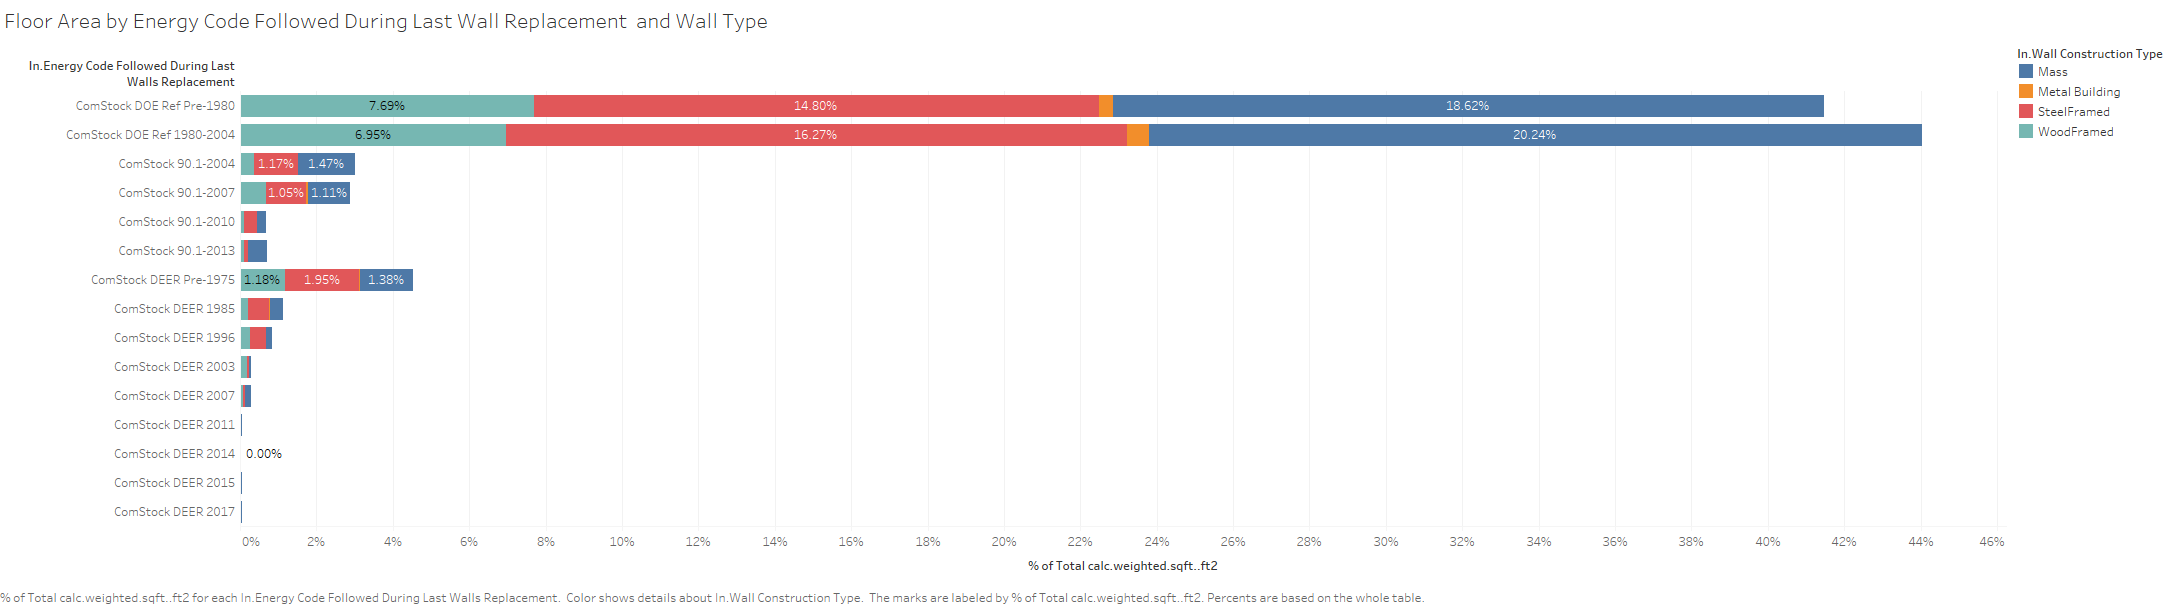
\includegraphics[
        page={1},
        trim={1cm 18.3cm 1cm 1cm}, clip, % L B R T
        width=\textwidth]{figures/weighted_floor_area_by_energy_code_and_wall_type.png}
    \caption[Weighted floor area by energy code followed during last wall replacement and wall type]{Weighted floor area by energy code followed during last wall replacement and wall type.}
    \label{fig:weighted_floor_area_by_energy_code_and_wall_type}
\end{figure}
\vspace{2mm}
\paragraph{Wall Thermal Performance}
We did not find any data sources that contained the thermal performance (U-Value/R-Value) of walls in the commercial building stock. This is likely because surveys would need to either find building plans, which can be difficult or impossible for older buildings, or disassemble part of the structure to look inside the walls, which building owners are unlikely to allow. To account for the lack of data, we estimated wall thermal performance based on an estimate of the energy code followed when the wall was last replaced. Section~\ref{sec:energy_code} describes how the energy code was determined. The thermal performance of walls for each energy code varies based on climate zone and construction type, as shown in Table~\ref{tab:wall_r_values} and Table~\ref{tab:wall_r_values_deer}. Note that although these thermal performance values do include the thermal bridging inherent in the clear field wall, they do not include thermal bridging at intermediate floors, parapets, and glazing transitions. These additional thermal bridges are expected to lower the overall thermal performance of the wall assembly.

As previously described, most of the building stock's walls are assumed to be older. Therefore, the thermal performance assumptions for older vintages have a much higher impact on the overall heating and cooling demand than those for newer vintages. The ComStock DOE Ref Pre-1980 assumptions, taken from \cite{doe_reference_buildings}, are originally from a study of only offices \citep{old_vintage_office_study}. Unfortunately, this study no longer appears to be available. Following the methodology in \cite{doe_reference_buildings}, these values are used for all wall construction types and all building types. Figure~\ref{fig:weighted_floor_area_by_building_type_and_wall_type} shows the final prevalence of each wall construction type by building type. Most notable is the low prevalence of metal building walls across the stock, even in warehouses. This might be surprising, but it is supported by the available data. Table \ref{tab:wall_r_value_averages} shows the average wall thermal performance by ASHRAE Standard 169--2006 climate zone.

\begin{figure}[ht!] \centering
    \includegraphics[
        page={2},
        trim={1cm 20.7cm 1cm 1cm}, clip, % L B R T
        width=\textwidth]{figures/weighted_floor_area_by_building_type_and_wall_type.png}
    \caption[Weighted floor area by wall type and building type]{Weighted floor area by wall type and building type.}
    \label{fig:weighted_floor_area_by_building_type_and_wall_type}
\end{figure}

\vspace{2mm}

\subsection{Windows} % Andrew
\paragraph{Window Construction Type}
Data from the NFRC Commercial Fenestration Market Study was used to develop the modeling approach for windows in ComStock. This study, conducted by Guidehouse in collaboration with NFRC, characterized the national commercial window stock through data collection and analysis. Six primary data sources representing all regions of the United States were used in the study---a 2020 Guidehouse survey, NEEA CBSA, DOE Code Study, CAEUS, CBECS, and RECS. A variety of window properties were collected, including the window-to-wall ratio, number of panes, frame material, glazing type, low-E coating, gas fill, solar heat gain coefficient (SHGC), U-factor, and many others. In total, the database contained approximately 16,000 samples, each with an appropriate weighting factor based on the coverage, completeness, and fidelity of each data source. The WWR data was already incorporated into the ComStock baseline during the EULP project. Some of the other key window properties such as thermal performance were then used to create the new baseline window constructions and distributions discussed later in this section. A summary of the data sources and their associated information is shown in Table ~\ref{tab:window_data_sources}.

Four window properties---number of panes, glazing type, frame material, and low-E coating---were used to create the baseline window configurations. These four parameters were selected based on which characteristics have the most impact on window performance, which have the most data available from the various data sources, and which inputs we trust from the average building owner or survey recipient. The options for each property are shown in Figure \ref{fig:window_configurations}.

\begin{figure}[ht!] \centering
    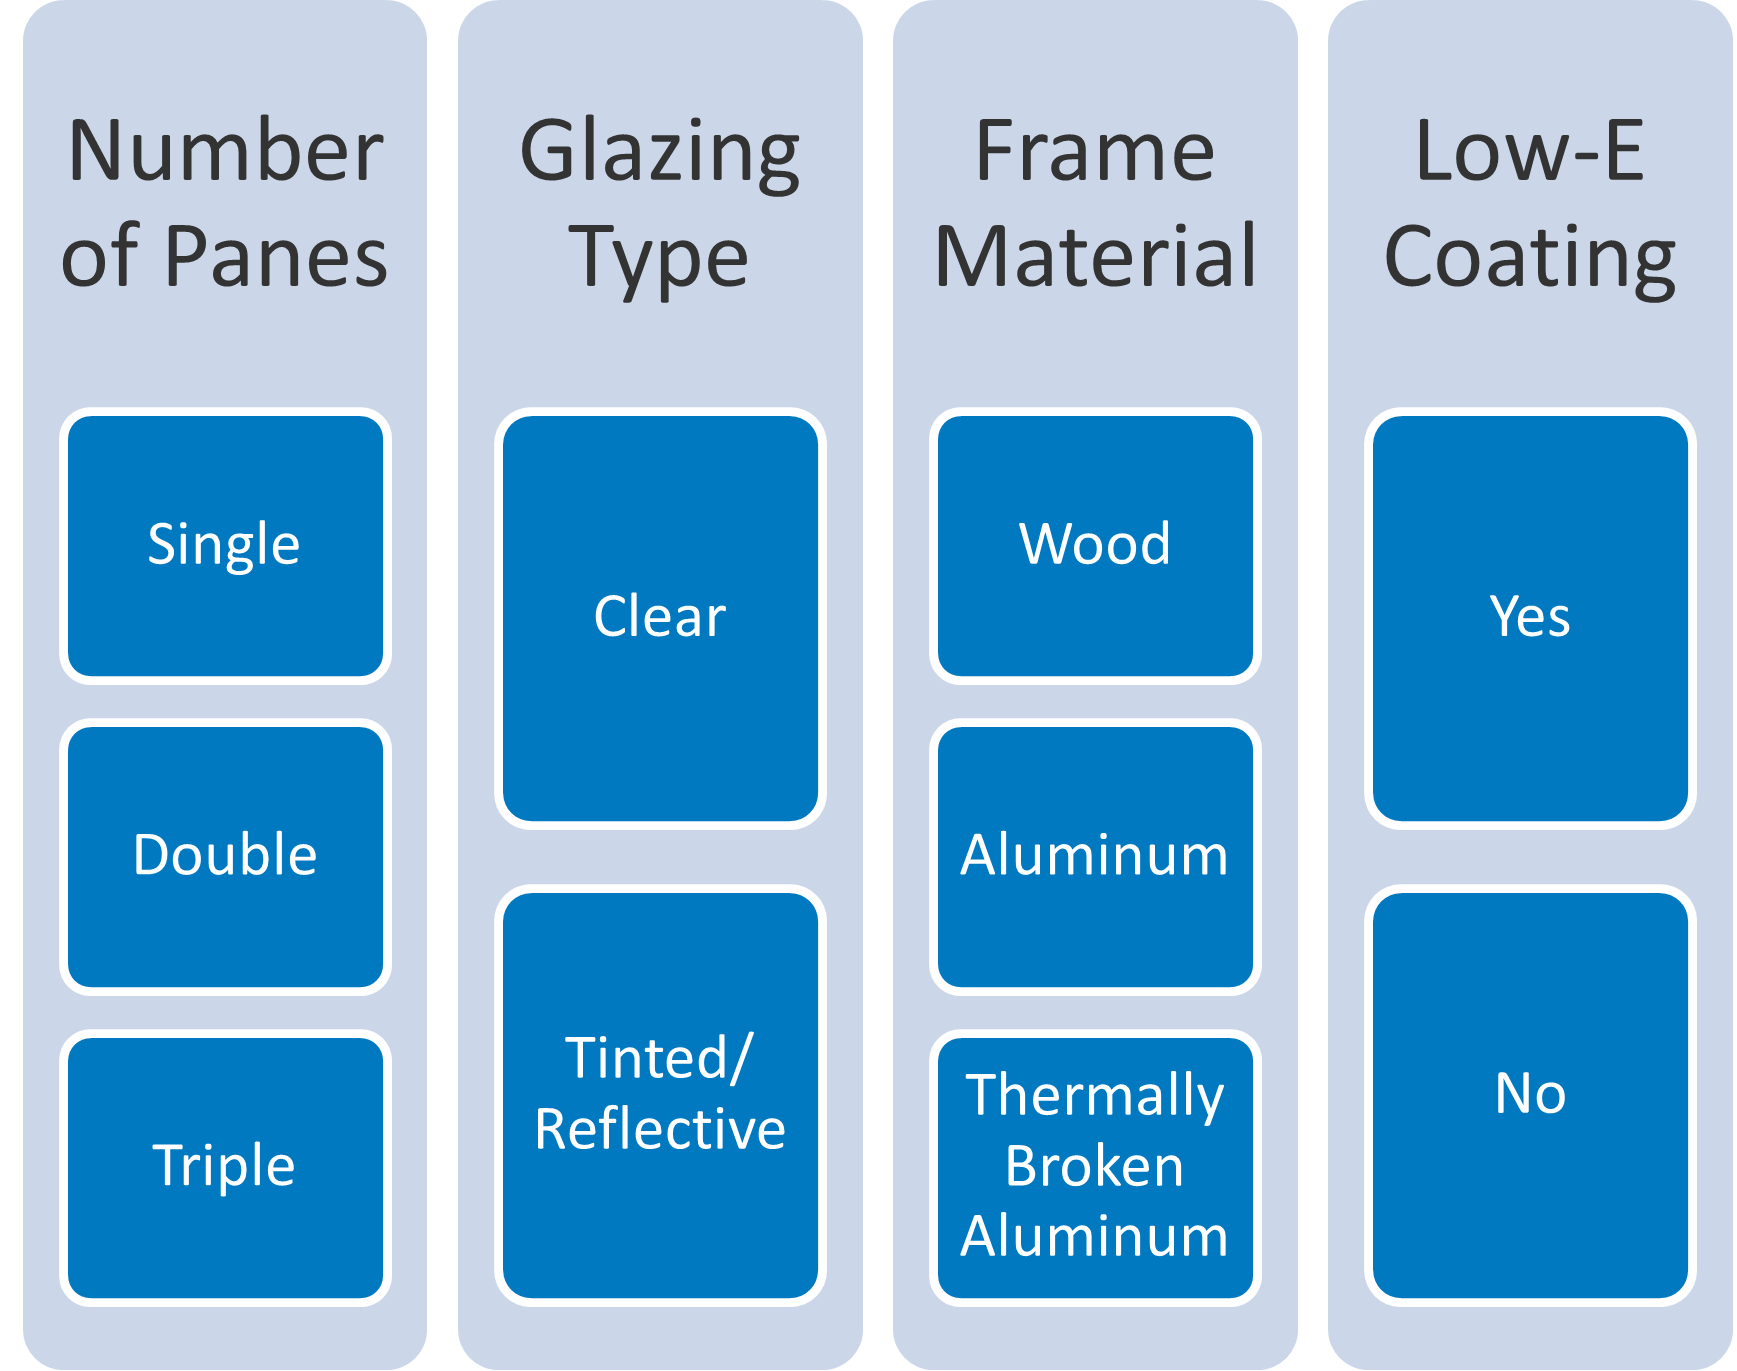
\includegraphics[
        trim={0cm 0cm 0cm 0cm}, clip, % L B R T
        width=0.5\textwidth]{figures/window_configurations.png}
    \caption{Window characteristics for number of panes, glazing type, frame material, and low-E coating.}
    \label{fig:window_configurations}
\end{figure}
\vspace{5mm}

Modeling every combination of these four properties would result in 36 different window configurations, which would add significant complexity to the sampling process. Instead, we selected 12 combinations to be modeled, based on which combinations are most common and most realistic. There are four single-pane, six double-pane, and two triple-pane configurations. The unrealistic/uncommon combinations that were eliminated include:
\begin{itemize}
\item Single pane with thermally broken aluminum frame
\item Single pane with low-E coating
\item Double pane with wood frame
\item Triple pane with no low-E coating
\item Triple pane without thermally broken aluminum frame
\item Thermally broken double or triple pane without low-E coating.
\end{itemize}
The 12 remaining window configurations are shown in Table \ref{tab:window_configurations}.

\begin{table}
\centering
\caption[Window Configurations]{Window Configurations}
\label{tab:window_configurations}
\begin{tabular}{|l|l|l|l|}
\hline
\textbf{Number of Panes} & \textbf{Glazing Type} & \textbf{Frame Material} & \textbf{Low-E Coating} \\ \hline
Single          & Clear             & Aluminum                    & No            \\ \hline
Single          & Tinted/Reflective & Aluminum                    & No            \\ \hline
Single          & Clear             & Wood                        & No            \\ \hline
Single          & Tinted/Reflective & Wood                        & No            \\ \hline
Double          & Clear             & Aluminum                    & No            \\ \hline
Double          & Tinted/Reflective & Aluminum                    & No            \\ \hline
Double          & Clear             & Aluminum                    & Yes           \\ \hline
Double          & Clear             & Aluminum With Thermal Break & Yes           \\ \hline
Double          & Tinted/Reflective & Aluminum                    & Yes           \\ \hline
Double          & Tinted/Reflective & Aluminum With Thermal Break & Yes           \\ \hline
Triple          & Clear             & Aluminum With Thermal Break & Yes           \\ \hline
Triple          & Tinted/Reflective & Aluminum With Thermal Break & Yes           \\ \hline
\end{tabular}
\end{table}

We created a sampling distribution for the new window constructions for the entire country using the initial data set. Overall, single-pane windows make up approximately 54\% of the stock, double-pane windows make up 46\%, and triple-pane windows make up <1\%. Initially, we created distributions based on census division to incorporate geographic location into the sampling. Upon further analysis, we found that it was also necessary to incorporate the energy codes into distributions to prevent scenarios where a single-pane window was sampled for a certain location, but, according to the energy code for that location, a double-pane window was required. For this reason, we modified the sampling distribution to include two dependencies---climate\_zone and  energy\_code\_followed\_during\_last\_window\_replacement.

To generate these sampling distributions, we used the maximum U-values specified for each climate zone in each version of ASHRAE 90.1, using climate zones defined by ASHRAE 169--2006. For each combination of climate zone and energy code, the 12 window configurations were evaluated to determine which were both realistic and met code (i.e., had a U-value lower than the code maximum U-value). For the older energy codes, we made several assumptions about technology adoption to determine which window configurations were realistic:
\begin{itemize}
    \item Low-E coating---not adopted until DOE Ref 1980--2004
    \item Thermally broken aluminum frame---not adopted until 90.1-2004
    \item Triple pane---not adopted until 90.1-2004.
\end{itemize}

Each combination of climate zone and energy code included 2--12 window configurations that met the criteria. After limiting the distributions to these configurations, we renormalized the percentages from the national distribution to 100\%. This kept the percentages from the national distribution while also incorporating intelligent assumptions based on climate zone and energy code. Table ~\ref{tab:window_distribution_4A} provides an example of the window configurations that were sampled for each code year in climate zone 4A.

\begin{table}
\scriptsize
\centering
\caption[Window Distribution Assumptions Example]{Window Distribution Assumptions Example from Climate Zone 4A}
\label{tab:window_distribution_4A}
\begin{tabular}{p{2.5in}|rrrrrr}
\textbf{Energy Code Followed During Last Windows Replacement}                      & \textbf{Pre-1980} & \textbf{1980-2004} & \textbf{90.1-2004} & \textbf{90.1-2007} & \textbf{90.1-2010} & \textbf{90.1-2013} \\
\textbf{Allowable Assembly Maximum U-Value}                                        & 1.22              & 0.59               & 0.57               & 0.55               & 0.55               & 0.42  \\
\textbf{Allowable Assembly Maximum SHGC}                                           & 0.54              & 0.36               & 0.39               & 0.4                & 0.4                & 0.4   \\ \hline
Single - No LowE - Clear - Aluminum \- U-1.178 SHGC-0.744                            & X                 &                    &                    &                    &                    &       \\ \hline
Single - No LowE - Tinted/Reflective - Aluminum \- U-1.178 SHGC-0.579                 & X                 &                    &                    &                    &                    &       \\ \hline
Single - No LowE - Clear - Wood \- U-0.91 SHGC-0.683                                  & X                 & X                  &                    &                    &                    &       \\ \hline
Single - No LowE - Tinted/Reflective - Wood \- U-0.91 SHGC-0.525                      & X                 & X                  &                    &                    &                    &       \\ \hline
Double - No LowE - Tinted/Reflective - Aluminum \- U-0.749 SHGC-0.484                 & X                 & X                  &                    &                    &                    &       \\ \hline
Double - No LowE - Clear - Aluminum \- U-0.746 SHGC-0.646                             & X                 & X                  &                    &                    &                    &       \\ \hline
Double - LowE - Clear - Aluminum \- U-0.559 SHGC-0.386                                &                   & X                  & X                  & X                  & X                  &       \\ \hline
Double - LowE - Tinted/Reflective - Aluminum \- U-0.557 SHGC-0.274                    &                   & X                  & X                  & X                  & X                  &       \\ \hline
Double - LowE - Clear - Thermally Broken Aluminum \- U-0.499 SHGC-0.378               &                   &                    & X                  & X                  & X                  & X     \\ \hline
Double - LowE - Tinted/Reflective - Thermally Broken Aluminum \- U-0.496 SHGC-0.266   &                   &                    & X                  & X                  & X                  & X     \\ \hline
Triple - LowE - Clear - Thermally Broken Aluminum \- U-0.3 SHGC-0.328                 &                   &                    & X                  & X                  & X                  & X     \\ \hline
Triple - LowE - Tinted/Reflective - Thermally Broken Aluminum \- U-0.299 SHGC-0.224   &                   &                    & X                  & X                  & X                  & X \\ \hline
& \multicolumn{6}{l}{X = This window type meets code minimums} \\
\end{tabular}
\end{table}

As can be seen in Table \ref{tab:window_distribution_4A}, for DOE Ref Pre-1980, the only windows that met code and are realistic are single-pane or double-pane windows with no low-E coating. For DOE Ref 1980--2004, the maximum U-value dropped significantly, such that single-pane aluminum windows no longer met code. However, double-pane low-E windows became available on the market at that time. For 90.1-2004 through 90.1-2010, code required a U-value equivalent to double-pane low-E or better, and in 90.1-2013, the code improved again, meaning that double-pane low-E with a thermal break or better was required. This type of logic was applied to all combinations of climate zone and energy code. Then, we converted the data into the distributions used in sampling.

A small adjustment was made to the final distributions because some states and localities do not follow or enforce energy codes strictly. Following the code exactly would likely overestimate window performance. Therefore, in scenarios where single-pane windows were technically below code, we assumed that 5\% of all windows in the stock would still have the worst-performing single-pane windows installed. The distributions were adjusted accordingly by subtracting 5\% total from the double-pane configurations and adding to the single-pane aluminum configurations. After making this manual adjustment, the new distributions had the same overall breakdown as the national distribution generated from the Guidehouse data---54\% single-pane and 46\% double-pane .

\paragraph{Window Thermal Performance}
Once the 12 new window constructions were determined, a team from Lawrence Berkeley National Laboratory's (LBNL’s) Windows and Daylighting Group used the WINDOW program to assign thermal performance properties to each construction. SimpleGlazing objects in EnergyPlus were chosen to represent windows to reduce complexity. This choice also simplifies the process of applying upgrades, because all fenestration objects in the baseline models use the same object type. The inputs for the SimpleGlazing object are U-factor, solar heat gain coefficient (SHGC), and visible light transmittance (VLT). For each window configuration, LBNL assigned a frame ID and window ID from the WINDOW database. They also filled in the respective U-factors, SHGCs, and VLTs, which are shown in Table \ref{tab:window_thermal_performance}.

The U-factors originally ranged from U-1.18 Btu/h·ft\textsuperscript{2}·F for the worst-performing single-pane window to U-0.30 Btu/h·ft\textsuperscript{2}·F for the best-performing triple-pane window. As mentioned earlier in this section, the maximum U-Factor that EnergyPlus can model with a simple glazing object is U-1.02 Btu/h·ft\textsuperscript{2}·F, which is governed by the limitations of a 2D heat transfer model when interior and exterior air films are included. Therefore, we adjusted the U-factor for the first two single-pane windows to be U-1.02 Btu/h·ft\textsuperscript{2}·F rather than U-1.18 Btu/h·ft\textsuperscript{2}·F. This allowed these windows to be modeled in ComStock. This results in a slight overestimate of the thermal performance of single-pane windows.


\subsection{Roof} % Andrew
\paragraph{Roof Construction Type}
First, we reviewed the general types of roof construction methods that could be represented. The three general roof types commonly used in commercial building energy codes were chosen because they cover the most common roof construction types and can be linked to nominal thermal characteristics. The definitions of these types from \cite{ashrae_901_2010} are as follows:

\begin{itemize}
\item \textbf{Roof with insulation entirely above deck (IEAD)}: A roof that has all insulation installed above (outside of) the roof structure and that is continuous (i.e., uninterrupted by framing members).
\item \textbf{Metal building roof}: A roof that is constructed with a metal, structural weathering surface; has no ventilated cavity; and has the insulation entirely below deck (i.e., does not include composite concrete and metal deck construction or a roof framing system that is separated from the superstructure by a wood substrate). In addition, the roof structure consists of one or
more of the following configurations: (a) metal roofing in direct contact with the steel framing members, (b) metal roofing separated from the steel framing members by insulation, or (c) insulated metal roofing panels installed as described in a or b.
\item \textbf{Attic and other roof}: All other roofs, including roofs with insulation entirely below (inside of) the roof structure (e.g., attics, cathedral ceilings, and single-rafter ceilings); roofs with insulation both above and below the roof structure; and roofs without insulation (excluding metal building roofs).
\end{itemize}

The analysis of roof properties in \cite{eia2012cbecs}, shown in Figure~\ref{fig:cbecs_floor_area_by_roof_tilt_and_attic_presence}, indicates that about 90\% of the commercial floor space covered by ComStock has flat or shallow pitch roofs, and that the large majority of the buildings with flat or shallow pitch roofs do not have attic space. Given these factors and the complexity associated with modeling the geometry of pitched roofs, we decided to model the entire stock as having flat roofs.

\begin{figure}[h] \centering
    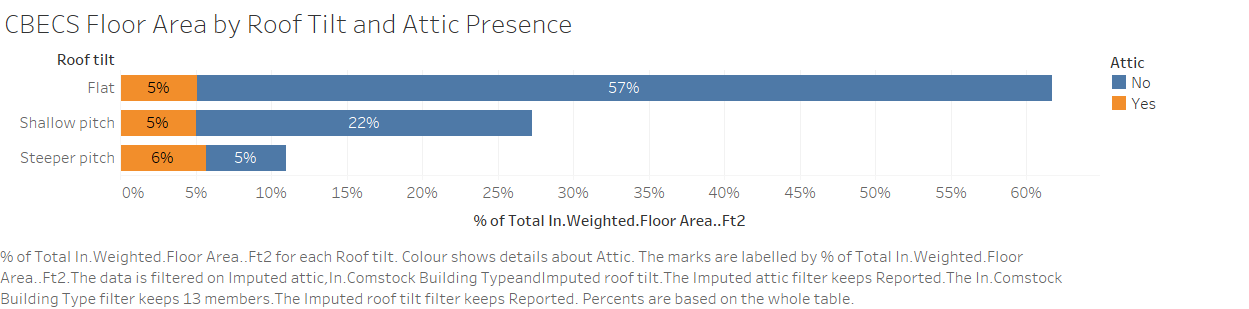
\includegraphics[
        trim={0cm 1.5cm 0cm 0cm}, clip, % L B R T
        width=\textwidth]{figures/cbecs_floor_area_by_roof_tilt_and_attic_presence.png}
    \caption{Weighted floor area by roof tilt and attic presence.}
    \label{fig:cbecs_floor_area_by_roof_tilt_and_attic_presence}
\end{figure}

\vspace{5mm}
No data sources for roof construction type were found. For buildings outside of California, a single roof construction type was chosen for each building type. As shown in Table~\ref{tab:roof_construction_types}, most buildings are assumed to use IEAD roofs, which is consistent with the assumption of flat roofs. For buildings in California, the construction types from the DEER prototype buildings were used \citep{cpuc_deer}.

\paragraph{Roof System Turnover Rate}
As described in Section \ref{sec:system_turnover_and_eul}, some building systems, including roofs, are assumed to be replaced over the lifespan of the building. Typically, for roofs, the structural elements are maintained, while the roof membrane and insulation are replaced. As noted in Section \ref{sec:system_turnover_and_eul}, the EUL for roofs was assumed to be 200 years, which means that most buildings are modeled with the roof insulation they were built with. Once the roof type probabilities and distribution of building types, sizes, and vintages are carried through the sampling process and simulations are created, the distribution of energy code levels can be reviewed. As shown in Figure~\ref{fig:weighted_floor_area_by_energy_code_roofs}, because the majority of the building stock is older, and roof systems are replaced at a low rate, most of the building floor area is assumed to have roofs that follow the oldest energy codes.

\begin{figure}[h] \centering
    \includegraphics[
        page={3},
        trim={1cm 20.5cm 1cm 1cm}, clip, % L B R T
        width=\textwidth]{figures/weighted_floor_area_by_energy_code_roofs.png}
    \caption{Weighted floor area by energy code followed during last roof replacement.}
    \label{fig:weighted_floor_area_by_energy_code_roofs}
\end{figure}
\vspace{5mm}
\paragraph{Roof Thermal Performance}
We did not find any data sources that contained the thermal performance (U-Value/R-Value) of roofs in the commercial building stock. This is likely because surveys would need to either find building plans, which can be difficult or impossible for older buildings, or disassemble part of the structure to look inside the roofs, which building owners are unlikely to allow. To account for the lack of data, we estimated roof thermal performance based on an estimate of the energy code followed when the roof was last replaced. Section~\ref{sec:energy_code} describes how the energy code was determined. The thermal performance of roofs for each energy code varies based on climate zone and construction type, as shown in Tables~\ref{tab:roof_r_values} and \ref{tab:roof_r_values_deer}. While these thermal performance values do include the thermal bridging inherent in the clear field roof, they do not include thermal bridging at parapets, skylight curbs, or roof penetrations for HVAC systems. These additional thermal bridges are expected to lower the overall thermal performance of the roof assembly.

As previously described, most of the building stock's roofs are assumed to be older. Therefore, the thermal performance assumptions for older vintages have a much higher impact on the overall heating and cooling demand than the assumptions for newer vintages. The ComStock DOE Ref Pre-1980 assumptions, taken from \cite{doe_reference_buildings}, are originally from a study of only offices \citep{old_vintage_office_study}. Unfortunately, this study no longer appears to be available. Following the methodology in \cite{doe_reference_buildings}, these values are used for all roof construction types and all building types.


\subsection{Floor}
In ComStock, all buildings are assumed to be built using slab-on-grade construction and to have no cantilevered thermal zones. Thus, the only heat transfer into the building through floors is assumed to happen through the floor in contact with the ground. All floors between stories are internal surfaces, and any heat transfer through these surfaces occurs between zones within the building, not between the building and the outside environment.

\paragraph{Floor Thermal Performance}
We did not find any data sources that contained the thermal performance of floors in the commercial building stock. This is likely because surveys would need to either find building plans, which can be difficult or impossible for older buildings, or excavate under a slab edge, which is impractical. To account for the lack of data, we estimated floor thermal performance based on an estimate of the energy code followed when building was first constructed. Section~\ref{sec:energy_code} describes how the energy code was determined. The thermal performance of floors for each energy code varies based on climate zone, as shown in Table~\ref{tab:floor_f_factors}. It is notable that only buildings built to the newest energy codes in the coldest climates assume any sort of slab insulation.

\subsection{Thermal Bridging} % Matthew Dahlhausen
Thermal bridging includes the impact of uninsulated structural elements that undermine the overall thermal resistance of an opaque assembly. These include linear thermal bridges, such as along corners, roof parapets, and fenestration, and point thermal bridges, such as protruding steel beams. These are formalized by psi factors multiplied by the length of a thermal bridge, and chi factors multiplied by the number of a thermal bridge. ASHRAE publishes psi and chi factors for common major thermal bridges, and thermal bridging requirements were recently added to the envelope section of ASHRAE 90.1-2022 \citep{ashrae_901_2022}. See Appendix section A10.2 of ASHRAE 90.1-2022 for details on calculating thermal bridges.

Thermal bridging in ComStock is implemented with the Thermal Bridging and Derating (TBD) ruby gem \citep{tbd_gem}. The gem detects the presence of common major thermal bridges in the model (corners, parapets, etc.), and derates the adjacent opaque surface construction (walls and roofs) to account for the thermal bridging. TBD gem version 3.4.1 includes default ASHRAE 90.1-2022 psi and chi factors for different kinds of thermal bridges. These vary by wall construction type (steel frame, mass, wood) and whether thermal bridges are considered mitigated or unmitigated. By default, ComStock assumed the unmitigated 90.1-2022 psi and chi factors by wall construction type. Specific values are listed in the TBD gem \citep{tbd_gem}.

\subsection{Infiltration and Natural Ventilation} % Matthew Dahlhausen

\subsubsection{Infiltration}
Infiltration in ComStock uses the same model as EnergyPlus \citep{energy_plus}, detailed in equation \ref{energyplus_infiltration_eqn}.

\begin{align}
\label{energyplus_infiltration_eqn}
Infiltration = I_{design} * F_{schedule} * [A + B * |(T_{zone} - T_{odb})| + C * WindSpeed + D * WindSpeed^2]
\end{align}

where:\\
\begin{itemize}
\item \textbf{I\textsubscript{design}} is the design infiltration flow rate, in m\textsuperscript{3} per s per m\textsuperscript{2} exterior surface area\\
\item \textbf{F\textsubscript{schedule}} is a fractional schedule, usually tied to HVAC system operation\\
\item \textbf{A} is the coefficient for constant infiltration\\
\item \textbf{B} is the coefficient for temperature difference driven infiltration\\
\item \textbf{T\textsubscript{zone}} is the zone air temperature, in degrees Celsius\\
\item \textbf{T\textsubscript{odb}}  is the outdoor dry bulb temperature, in degrees Celsius\\
\item \textbf{C} and \textbf{D} are linear and quadratic coefficients for wind driven infiltration\\
\item \textbf{WindSpeed} is the local windspeed, in m per s.\\
\end{itemize}

The selection of the design infiltration rate is somewhat arbitrary, as it depends on the assumed natural pressure at typical conditions. The coefficients need to be paired with an assumed natural pressure.

\subsubsection{Infiltration Rates}
Infiltration rates are calculated from measured airtightness data from \citep{nist_infiltration_data}. There are significant differences in building airtightness due to differences in wall construction, shown in Figure 6 of the NIST reference. Airtightness does not vary significantly by building type or vintage. Airtightness does depend on size, but this is inherently captured by larger buildings having smaller surface area to volume ratios. Air barriers greatly reduce leakiness, but they are rare in existing buildings, and only recently have been required in some jurisdictions. Airtightness of buildings in ComStock follow lognormal distributions with airtightness means by wall construction type matched to those in \citep{nist_infiltration_data}, shown in Figure \ref{fig:airtightness_by_wall_construction_type}.
Airtightness values are measured at 75 Pa and are 6-sided, meaning the infiltration is normalized by total building exterior surface area including wall, roof, and ground surfaces.

The design infiltration rate is calculated from the airtightness value assuming a 4 Pa design pressure, shown in \ref{airtightness_to_design_infiltration}
\begin{align}
\label{airtightness_to_design_infiltration}
I_{\text{design}} = \text{airtightness} \cdot \left(\frac{1\ \text{hr}}{3600\ \text{s}}\right) \cdot \left(\frac{5\ \text{sided area}}{6\ \text{sided area}}\right) \cdot \left(\frac{4.0\ \text{Pa}}{75.0\ \text{Pa}}\right)^{0.65}
\end{align}
where:\\
\begin{itemize}
\item \textbf{airtightness} is the measured airtightness at 75 Pa in m\textsuperscript{3} per hr per m\textsuperscript{2} 6-sided exterior surface area\\
\item \textbf{I\textsubscript{design}} is the design infiltration rate at 4 Pa in m\textsuperscript{3} per s per m\textsuperscript{2} 5-sided exterior surface area\\
\end{itemize}

\begin{figure}
    \centering 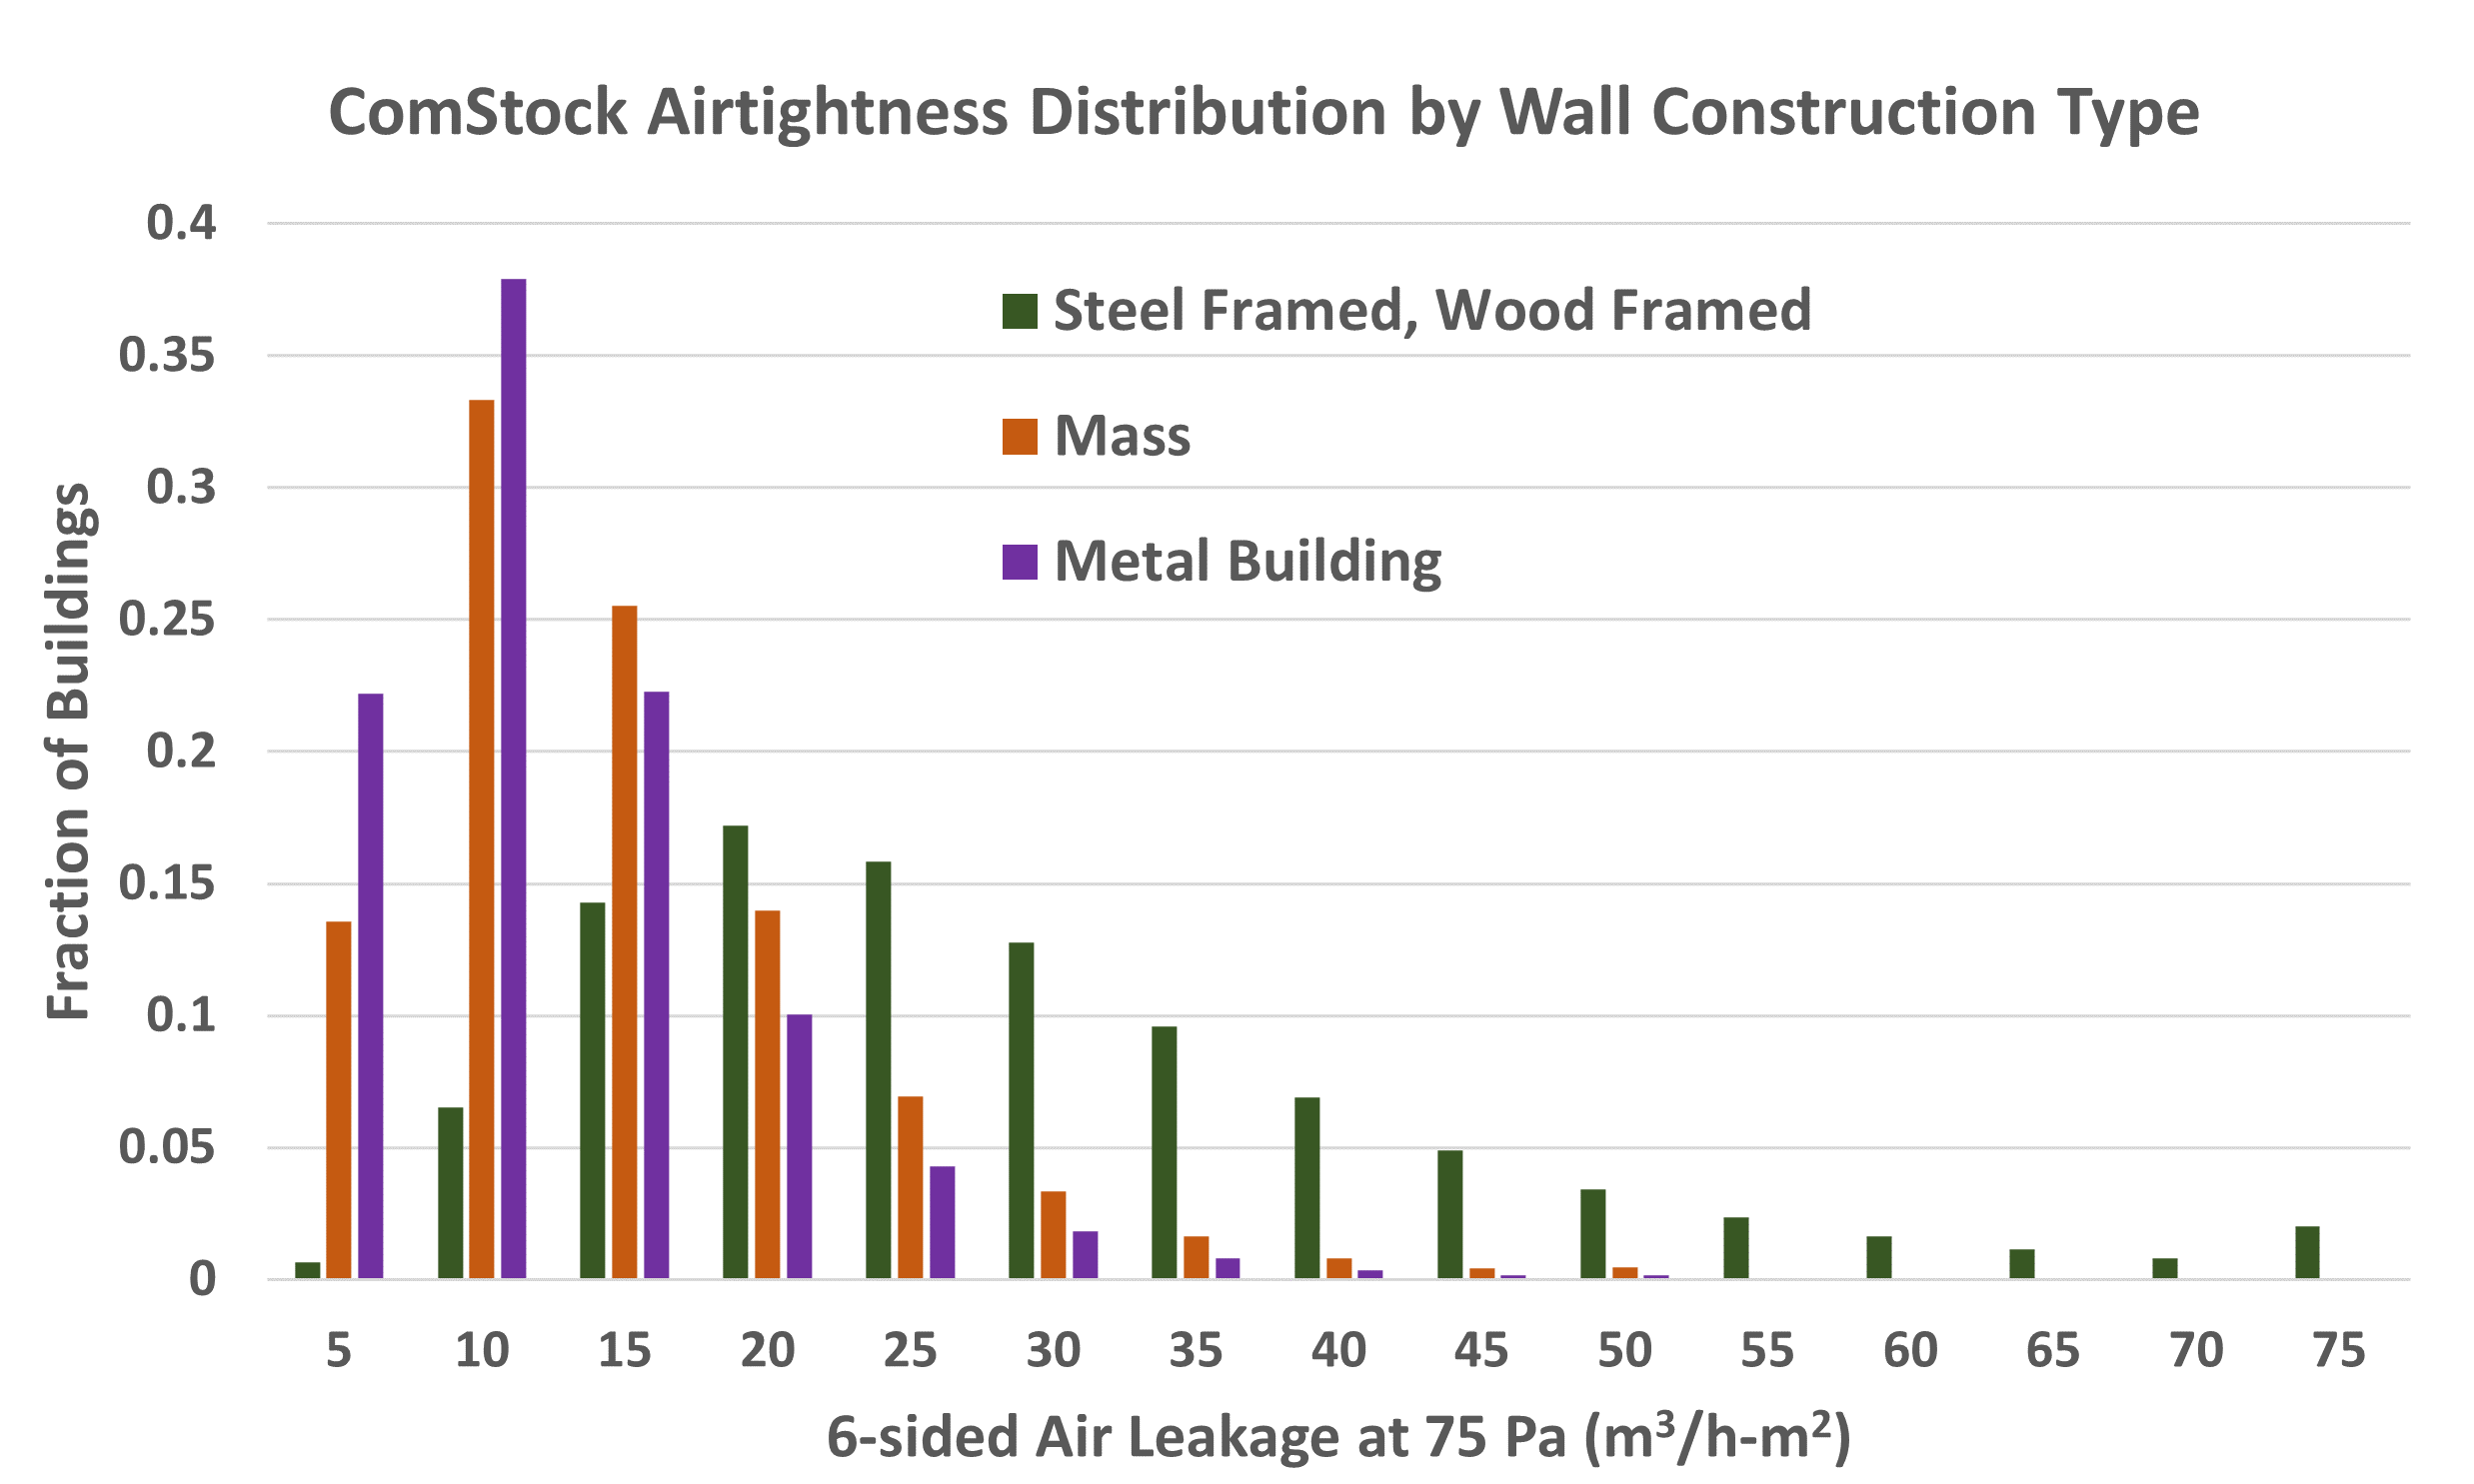
\includegraphics[width=0.9\textwidth]{figures/airtightness_by_wall_construction_type.png}
    \caption[Airtightness by Wall Construction Type]{6-sided airtightness distributions by wall construction type. Distributions are lognormal, with means matched to means by wall construction type in \citep{nist_infiltration_data}.}
    \label{fig:airtightness_by_wall_construction_type}
\end{figure}

\subsubsection{Infiltration Coefficients}
NIST derived coefficients by building CONTAM models of all of the DOE prototype buildings, as explained in \citep{nist_infiltration_correlations}. The coefficients assume a 4 Pa design pressure. The coefficients include A, B, and D terms, with C being 0. Coefficients are by building type, with separate coefficients for whether the HVAC system is on or off. The NIST report includes separate coefficients for buildings with air barriers, but ComStock does not assume buildings have air barriers.

NIST did not model all DOE prototype buildings, and does not include HVAC system off coefficients for some buildings if the prototype was modeled as always on. ComStock building types not available in the NIST data use coefficients for either the Office or Retail building types. If off coefficients are not available, the building uses the on coefficients instead.
\subsubsection{Natural Ventilation}

Natural ventilation is not modeled in ComStock because it is not common in the building stock.

\section{Lighting}
\subsection{Interior Lighting}
Interior lighting follows a technology baseline approach, meaning that energy consumed by lighting is set by an assumed distribution of a particular lighting technology (e.g., T8 or linear LEDs), rather than following a lighting power density (LPD) allowance defined in a specific energy code version. The technology baseline approach recognizes that buildings typically do not use their full lighting power allowance. It also explicitly labels lighting technology and subsystems in the energy model for granular energy efficiency measure analysis.  

Two components specify interior lighting: the lighting power density and the interior lighting schedule.  The lighting power density is determined by the distribution of lighting technologies in the stock, the lighting technology properties, and the space type properties. The lighting schedule is determined by a default lighting schedule by space type, occupancy hour adjustments, and magnitude variability.

\subsubsection{Determining Lighting Power}
The technology baseline approach follows a similar process to how the ASHRAE 90.1 lighting subcommittee determines the LPD allowance for a given space type in ASHRAE 90.1. In the lighting subcommittee model (LSM), there are four kinds of lighting systems that together contribute to a target horizontal illuminance:

LPD = General Lighting + Task Lighting + Supplemental Lighting + Wall Wash Lighting \\

\begin{align}
\label{lsm_lpd_eqn}
LPD = \frac{\% LS_{1} \cdot fc}{RSDD \cdot TF_{1}} + \frac{\% LS_{2} \cdot fc}{RSDD \cdot TF_{2}} + \frac{\% LS_{3} \cdot fc}{RSDD \cdot TF_{3}} + \frac{\% LS_{4} \cdot fc}{RSDD \cdot TF_{4}}
\end{align}
where:\\
\begin{itemize}
\item \textbf{\%LS\textsubscript{i}} is the percent of the target horizontal illuminance value met by a specific lighting system\\
\item \textbf{fc} is the target horizontal illuminance value in lumens per ft\textsuperscript{2}\\
\item \textbf{RSDD} is room surface dirt depreciation, an estimate of how much surface dirt reduces light from reaching the horizontal plane\\
\item \textbf{TF\textsubscript{i}} is the total lighting factor, where TF = source luminous efficacy * coefficient of utilization * lighting loss factor (LFF)\\
\item \textbf{Source luminous efficacy} is the lighting technology efficacy in lumens per watt\\
\item \textbf{Coefficient of utilization} is a term that captures how much lighting from the luminaire reaches the horizontal plane\\
\item \textbf{LLF} is the lighting loss factor, where LLF  = luminaire dirt depreciation (LDD) * lamp lumen depreciation (LLD)\\
\end{itemize}

Values for all these terms are specified in the LSM.  The LSM is exact, using a specific lighting product, room geometry, distribution of lighting systems, and other properties to determine the lighting power density allowance for a given space type. ComStock differs from the LSM in several important ways. 

First, ComStock generalizes lighting technology (e.g., T8 linear fluorescent luminaires for general lighting) rather than modeling a specific lighting product.  Source efficacy, lighting loss properties, and radiant fractions are tied to lighting technology. Source efficacy values come from \cite{doe2015lmc} for older lighting technologies and \cite{doe2019ssl} for LEDs.  Radiant heat gain fractions come from \cite{ashrae_rp1282} for older lighting technologies and \cite{ashrae_rp1681} for LEDs.

Second, lighting technologies are broken out into lighting generations depending on the most common space lighting technology in that generation, as general lighting accounts for most ($\sim$80\%--90\%) of total lighting. High bay is treated as general lighting, and the lighting measure uses the general high bay technology for rooms with height $\ge$20 ft. Lighting generations 4--8 are all LED, with improving efficacy over time. Lighting generations and their technologies are detailed in Table \ref{tab:int_light_gens}, and lighting technology properties are detailed in Table~\ref{tab:int_light_techs_all}.

%\begin{center}
\begin{landscape}
  \scriptsize
  \begin{longtable}{|p{0.75in}|p{0.65in}|p{0.47in}|p{0.4in}|p{0.45in}|p{0.4in}|p{0.4in}|p{0.4in}|p{0.4in}|p{0.4in}|p{0.4in}|p{0.4in}|p{0.4in}|p{0.4in}|}
  \caption[Interior Lighting Technologies]{Interior Lighting Technologies} \\ \hline
  \label{tab:int_light_techs_all}
  \textbf{Lighting Technology}        & \textbf{Generation}              & \textbf{System Type}            & \textbf{Fixture Type}  & \textbf{Lamp Type}              & \textbf{Fixture Min. Height (ft)} & \textbf{Fixture Max. Height (ft)} & \textbf{Source Efficacy (lumens/Watt)} & \textbf{Lamp Lumen Depreciation} & \textbf{Luminaire Dirt Depreciation} & \textbf{Lighting Loss Factor} & \textbf{Return Air Fraction} & \textbf{Radiant Fraction} & \textbf{Visible Fraction} \\ \hline
  \endfirsthead
  \multicolumn{2}{c} {{\textbf{\textit{Continued from previous page}}}} \\ \hline
  \textbf{Lighting Technology}        & \textbf{Generation}              & \textbf{System Type}            & \textbf{Fixture Type}  & \textbf{Lamp Type}              & \textbf{Fixture Min. Height (ft)} & \textbf{Fixture Max. Height (ft)} & \textbf{Source Efficacy (lumens/Watt)} & \textbf{Lamp Lumen Depreciation} & \textbf{Luminaire Dirt Depreciation} & \textbf{Lighting Loss Factor} & \textbf{Return Air Fraction} & \textbf{Radiant Fraction} & \textbf{Visible Fraction} \\ \hline
  \endhead
  T12                        & gen1\_t12\_incandescent & general                & lamp          & fluorescent             & 0                     & 20                    & 74                              & 0.93                    & 0.89                        & 0.8277               & 0                   & 0.31             & 0.2              \\ \hline
  HID High Bay Mercury Vapor & gen1\_t12\_incandescent & general                & luminaire     & HID                     & 20                    & 1,000                  & 43                              & 0.88                    & 0.74                        & 0.6512               & 0                    & 0.465           & 0.2              \\ \hline
  Incandescent Decorative    & gen1\_t12\_incandescent & supplemental           & luminaire     & incandescent            & 0                     & 1,000                  & 8.7                             & 0.97                    & 0.83                        & 0.8051               & 0                   & 0.125            & 0.2              \\ \hline
  Incandescent A-Shape       & gen1\_t12\_incandescent & task                   & lamp          & incandescent            & 0                     & 1,000                  & 10.3                            & 0.97                    & 0.81                        & 0.7857               & 0                   & 0.125            & 0.2              \\ \hline
  Incandescent Decorative    & gen1\_t12\_incandescent & wall wash              & luminaire     & incandescent            & 0                     & 1,000                  & 8.7                             & 0.97                    & 0.81                        & 0.7857               & 0                   & 0.125            & 0.2              \\ \hline
  T8                         & gen2\_t8\_halogen       & general                & lamp          & fluorescent             & 0                     & 20                    & 94.1                            & 0.93                    & 0.89                        & 0.8277               & 0                   & 0.31             & 0.2              \\ \hline
  HID High Bay Metal Halide  & gen2\_t8\_halogen       & general                & luminaire     & HID                     & 20                    & 1,000                  & 90.2                            & 0.88                    & 0.74                        & 0.6512               & 0                   & 0.465            & 0.2              \\ \hline
  Halogen Decorative         & gen2\_t8\_halogen       & supplemental           & luminaire     & halogen                 & 0                     & 1,000                  & 15                              & 0.97                    & 0.83                        & 0.8051               & 0                   & 0.125            & 0.2              \\ \hline
  Halogen A-Shape            & gen2\_t8\_halogen       & task                   & lamp          & halogen                 & 0                     & 1,000                  & 17.5                            & 0.97                    & 0.81                        & 0.7857               & 0                   & 0.125            & 0.2              \\ \hline
  Halogen Decorative         & gen2\_t8\_halogen       & wall wash              & luminaire     & halogen                 & 0                     & 1,000                  & 15                              & 0.97                    & 0.81                        & 0.7857               & 0                   & 0.125            & 0.2              \\ \hline
  T5                         & gen3\_t5\_cfl           & general                & lamp          & fluorescent             & 0                     & 20                    & 103.5                           & 0.93                    & 0.89                        & 0.8277               & 0                   & 0.31             & 0.2              \\ \hline
  HID High Bay Metal Halide  & gen3\_t5\_cfl           & general                & luminaire     & HID                     & 20                    & 1,000                  & 90.2                            & 0.88                    & 0.74                        & 0.6512               & 0                   & 0.465            & 0.2              \\ \hline
  Compact Fluorescent Pin    & gen3\_t5\_cfl           & supplemental           & luminaire     & CFL                     & 0                     & 1,000                  & 70.1                            & 0.85                    & 0.83                        & 0.7055               & 0                   & 0.35             & 0.2              \\ \hline
  Compact Fluorescent Screw  & gen3\_t5\_cfl           & task                   & lamp          & CFL                     & 0                     & 1,000                  & 62.4                            & 0.85                    & 0.81                        & 0.6885               & 0                   & 0.35             & 0.2              \\ \hline
  Compact Fluorescent Pin    & gen3\_t5\_cfl           & wall wash              & luminaire     & CFL                     & 0                     & 1,000                  & 70.1                            & 0.85                    & 0.81                        & 0.6885               & 0                   & 0.35             & 0.2              \\ \hline
  LED Lamp Linear            & gen4\_led               & general                & lamp          & LED                     & 0                     & 20                    & 104                             & 0.85                    & 0.87                        & 0.7395               & 0                   & 0.365            & 0.2              \\ \hline
  LED Luminaire              & gen4\_led               & general                & luminaire     & LED                     & 0                     & 20                    & 96                              & 0.85                    & 0.85                        & 0.7225               & 0                   & 0.365            & 0.2              \\ \hline
  LED High Bay Luminaire     & gen4\_led               & general                & luminaire     & LED                     & 20                    & 1,000                  & 118                             & 0.85                    & 0.75                        & 0.6375               & 0                   & 0.465            & 0.2              \\ \hline
  LED Decorative             & gen4\_led               & supplemental           & luminaire     & LED                     & 0                     & 1,000                  & 87                              & 0.85                    & 0.9                         & 0.765                & 0                   & 0.165            & 0.2              \\ \hline
  LED Lamp General Purpose   & gen4\_led               & task                   & lamp          & LED                     & 0                     & 1,000                  & 93                              & 0.85                    & 0.87                        & 0.7395               & 0                   & 0.165            & 0.2              \\ \hline
  LED Directional            & gen4\_led               & wall wash              & luminaire     & LED                     & 0                     & 1,000                  & 51                              & 0.85                    & 0.84                        & 0.714                & 0                   & 0.165            & 0.2              \\ \hline
  LED Lamp Linear            & gen5\_led               & general                & lamp          & LED                     & 0                     & 20                    & 116                             & 0.85                    & 0.87                        & 0.7395               & 0                   & 0.365            & 0.2              \\ \hline
  LED Luminaire              & gen5\_led               & general                & luminaire     & LED                     & 0                     & 20                    & 109                             & 0.85                    & 0.85                        & 0.7225               & 0                   & 0.365            & 0.2              \\ \hline
  LED High Bay Luminaire     & gen5\_led               & general                & luminaire     & LED                     & 20                    & 1,000                  & 132                             & 0.85                    & 0.75                        & 0.6375               & 0                   & 0.465            & 0.2              \\ \hline
  LED Decorative             & gen5\_led               & supplemental           & luminaire     & LED                     & 0                     & 1,000                  & 97                              & 0.85                    & 0.9                         & 0.765                & 0                   & 0.165            & 0.2              \\ \hline
  LED Lamp General Purpose   & gen5\_led               & task                   & lamp          & LED                     & 0                     & 1,000                  & 105                             & 0.85                    & 0.87                        & 0.7395               & 0                   & 0.165            & 0.2              \\ \hline
  LED Directional            & gen5\_led               & wall wash              & luminaire     & LED                     & 0                     & 1,000                  & 57                              & 0.85                    & 0.84                        & 0.714                & 0                   & 0.165            & 0.2              \\ \hline
  LED Lamp Linear            & gen6\_led               & general                & lamp          & LED                     & 0                     & 20                    & 132                             & 0.85                    & 0.87                        & 0.7395               & 0                   & 0.365            & 0.2              \\ \hline
  LED Luminaire              & gen6\_led               & general                & luminaire     & LED                     & 0                     & 20                    & 126                             & 0.85                    & 0.85                        & 0.7225               & 0                   & 0.365            & 0.2              \\ \hline
  LED High Bay Luminaire     & gen6\_led               & general                & luminaire     & LED                     & 20                    & 1,000                  & 152                             & 0.85                    & 0.75                        & 0.6375               & 0                   & 0.465            & 0.2              \\ \hline
  LED Decorative             & gen6\_led               & supplemental           & luminaire     & LED                     & 0                     & 1,000                  & 111                             & 0.85                    & 0.9                         & 0.765                & 0                   & 0.165            & 0.2              \\ \hline
  LED Lamp General Purpose   & gen6\_led               & task                   & lamp          & LED                     & 0                     & 1,000                  & 122                             & 0.85                    & 0.87                        & 0.7395               & 0                   & 0.165            & 0.2              \\ \hline
  LED Directional            & gen6\_led               & wall wash              & luminaire     & LED                     & 0                     & 1,000                  & 64                              & 0.85                    & 0.84                        & 0.714                & 0                   & 0.165            & 0.2              \\ \hline
  LED Lamp Linear            & gen7\_led               & general                & lamp          & LED                     & 0                     & 20                    & 145                             & 0.85                    & 0.87                        & 0.7395               & 0                   & 0.365            & 0.2              \\ \hline
  LED Luminaire              & gen7\_led               & general                & luminaire     & LED                     & 0                     & 20                    & 140                             & 0.85                    & 0.75                        & 0.6375               & 0                   & 0.365            & 0.2              \\ \hline
  LED High Bay Luminaire     & gen7\_led               & general                & luminaire     & LED                     & 20                    & 1,000                  & 167                             & 0.85                    & 0.75                        & 0.6375               & 0                   & 0.465            & 0.2              \\ \hline
  LED Decorative             & gen7\_led               & supplemental           & luminaire     & LED                     & 0                     & 1,000                  & 123                             & 0.85                    & 0.9                         & 0.765                & 0                   & 0.165            & 0.2              \\ \hline
  LED Lamp General Purpose   & gen7\_led               & task                   & lamp          & LED                     & 0                     & 1,000                  & 136                             & 0.85                    & 0.87                        & 0.7395               & 0                   & 0.165            & 0.2              \\ \hline
  LED Directional            & gen7\_led               & wall wash              & luminaire     & LED                     & 0                     & 1,000                  & 71                              & 0.85                    & 0.84                        & 0.714                & 0                   & 0.165            & 0.2              \\ \hline
  LED Lamp Linear            & gen8\_led               & general                & lamp          & LED                     & 0                     & 20                    & 157                             & 0.85                    & 0.87                        & 0.7395               & 0                   & 0.365            & 0.2              \\ \hline
  LED Luminaire              & gen8\_led               & general                & luminaire     & LED                     & 0                     & 20                    & 152                             & 0.85                    & 0.75                        & 0.6375               & 0                   & 0.365            & 0.2              \\ \hline
  LED High Bay Luminaire     & gen8\_led               & general                & luminaire     & LED                     & 20                    & 1,000                  & 181                             & 0.85                    & 0.75                        & 0.6375               & 0                   & 0.465            & 0.2              \\ \hline
  LED Decorative             & gen8\_led               & supplemental           & luminaire     & LED                     & 0                     & 1,000                  & 133                             & 0.85                    & 0.9                         & 0.765                & 0                   & 0.165            & 0.2              \\ \hline
  LED Lamp General Purpose   & gen8\_led               & task                   & lamp          & LED                     & 0                     & 1,000                  & 147                             & 0.85                    & 0.87                        & 0.7395               & 0                   & 0.165            & 0.2              \\ \hline
  LED Directional            & gen8\_led               & wall wash              & luminaire     & LED                     & 0                     & 1,000                  & 76                              & 0.85                    & 0.84                        & 0.714                & 0                   & 0.165            & 0.2              \\ \hline
  \multicolumn{5}{l}{Lighting loss factor reference: PNNL 90.1 lighting subcommittee model} \\
  \multicolumn{5}{l}{Source efficacy reference, gen1--gen3: DOE 2015 LMC Table C3} \\
  \multicolumn{5}{l}{Source efficacy reference, gen4--gen8: DOE 2019 SSL Table D4} \\
  \multicolumn{5}{l}{Radiant fraction references: ASHRAE RP 1282 and ASHRAE RP 1681} \\
  \end{longtable}
  \end{landscape}
  \end{center}
  

Third, the coefficient of utilization depends on both the luminaire properties and the room geometry, which complicates the calculation in the LSM. The ComStock model associates the coefficient of utilization entirely with room propertiesthat are independent of lighting technology.  ComStock further assumes that rooms of the same space type have similar enough properties that they can use the same coefficient of utilization. To retain some of the variation from the luminaire properties, each kind of lighting system has a different coefficient of utilization for each space type. 

Table~\ref{tab:int_light_space_types} in Appendix~\ref{appendix:a} details the target horizontal illuminance value, the fraction of the target illuminance met by the kind of lighting system, and the lighting system coefficient of utilization for each lighting space type. Lighting space types are defined in 90.1 and are determined based on a mapping of openstudio-standards space types to prototype lighting space types.

Fourth, the LSM assumes a high fraction of non-general lighting systems for certain space types. For example, half of the illuminance in retail sales spaces is from supplemental and wall wash lighting systems. In older lighting generations, there is a significant difference in source efficacy between general and non-general lighting systems. In lighting generation 2, general lighting assumes T8 linear fluorescent lamps at 94 lumens per watt, and supplemental and wall wash lighting assume halogens at 15 lumens per watt.  For retail spaces using the LSM values, that means half the lighting comes from lighting technologies roughly 6 times less efficient than the general lighting technology.  Although this may be appropriate for setting a code lighting allowance, most retail spaces meet a much greater percentage of their illuminance from more efficient general lighting technologies.  ComStock adjusts the lighting system fractions for commonly used space types so that around 80\%--90\% of lighting comes from the general lighting system. These changes are reflected in Table~\ref{tab:int_light_space_types} in Appendix \ref{appendix:a}.

Lastly, the LSM offers a generous allowance for lighting power density to account for the lighting loss factor over time. Including lighting losses and depreciation can result in a lighting power density ~40\% higher than when these terms are ignored. This resulted in unreasonably high installed lighting power densities; thus, ComStock assumes that most existing lighting systems were not designed to account for depreciation over time, and therefore excludes lighting loss and depreciation terms from the lighting power calculation.

With these changes, the LPD calculation simplifies to:
\begin{align}
\label{comstock_lpd_eqn}
LPD = \frac{\% LS_{1} \cdot fc}{\text{efficacy} \cdot CU_{1}} + \frac{\% LS_{2} \cdot fc}{\text{efficacy} \cdot CU_{2}} + \frac{\% LS_{3} \cdot fc}{\text{efficacy} \cdot CU_{3}} + \frac{\% LS_{4} \cdot fc}{\text{efficacy} \cdot CU_{4}}
\end{align}

where:\\
\begin{itemize}
\item \textbf{\%LS\textsubscript{i}} is the percent of the target horizontal illuminance value met by a specific lighting system\\
\item \textbf{fc} is the target horizontal illuminance value in lumens per ft\textsuperscript{2}\\
\item \textbf{Efficacy} is the source luminous efficacy of the lighting technology in lumens per watt\\
\item \textbf{CU} is the coefficient of utilization, a term that captures how much lighting from the luminaire reaches the horizontal plane.\\
\end{itemize}

The resulting LPDs are shown in Figure~\ref{fig:interior_lighting_lpd}.

\begin{table}
\small
\centering
\caption[Interior Lighting Generations and Technologies]{Interior Lighting Generations and Technologies}
\label{tab:int_light_gens}
\begin{tabular}{p{0.5in}p{1in}p{1in}p{1in}p{1in}p{1in}}
\hline
\textbf{Lighting Generation} & \textbf{General Lighting Technology} & \textbf{General Lighting (High Bay) Technology} & \textbf{Task Lighting Technology} & \textbf{Supplemental Lighting Technology} & \textbf{Wall Wash Lighting Technology} \\
\hline \\
Gen 1 & T12 Linear Fluorescent & HID Mercury Vapor & Incandescent A-Shape & Incandescent Decorative & Incandescent Decorative \\ \hline
Gen 2 & T8 Linear Fluorescent & HID Metal Halide & Halogen A-Shape & Halogen Decorative & Halogen Decorative \\ \hline
Gen 3 & T5 Linear Fluorescent & HID Metal Halide & Compact Fluorescent Screw & Compact Fluorescent Pin & Compact Fluorescent Pin \\ \hline
Gen 4--8 & LED Linear & LED High Bay Luminaire & LED General Purpose & LED Decorative & LED Directional \\ \hline
\end{tabular}
\end{table}

\begin{figure}
    \centering 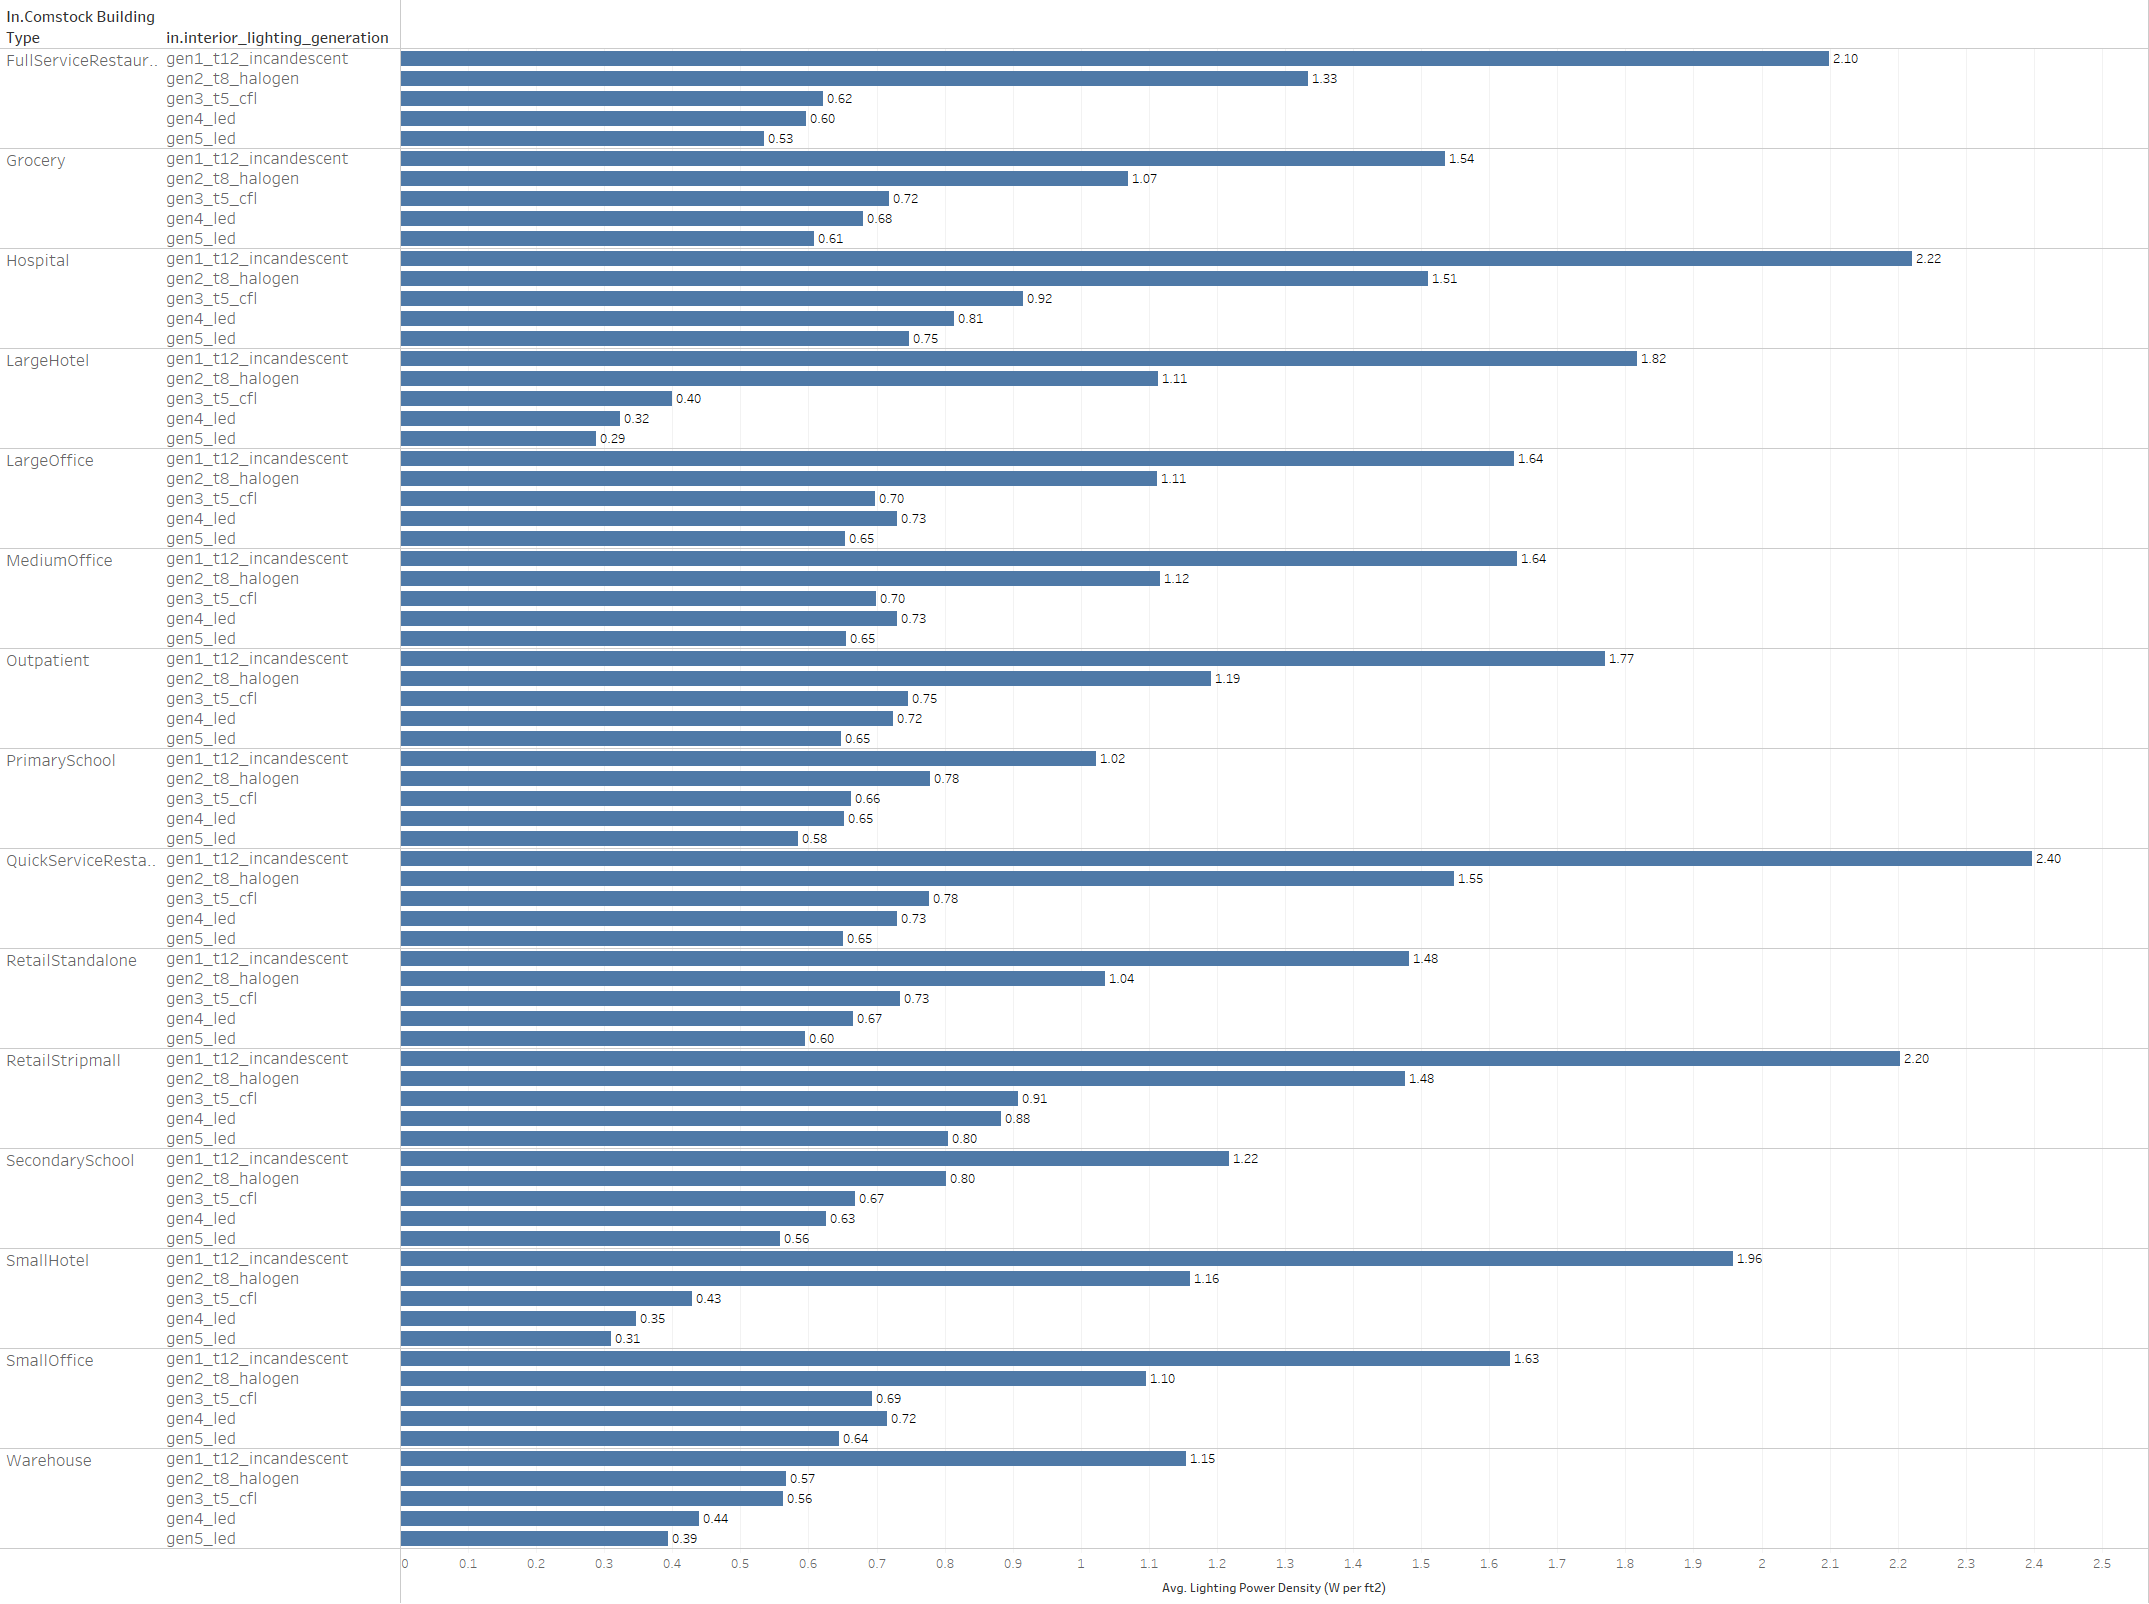
\includegraphics[width=1\textwidth]{figures/interior_lighting_lpd.png}
    \caption[Average interior lighting power density by building type and lighting generation]{Average interior lighting power density by building type and lighting generation.}
    \label{fig:interior_lighting_lpd}
\end{figure}

\pagebreak
\subsubsection{Distribution of Lighting Technologies}

Lighting generations were assigned to each building model during sampling based on the year of, and energy code in force during, the last interior lighting replacement.  Probability distributions were generated first by using an approximate start and end year for when each technology generation was being installed in commercial buildings (Table \ref{tab:ltg_gen_year}). A Gaussian distribution was generated for each lighting generation using these start and end years, and the resulting distribution for each year of last interior lighting replacement was normalized to create 0--1 probabilities. The probability distributions were duplicated for each energy code in force and were further modified to ensure they were realistic (i.e., generation 1 was not installed in a ComStock 90.1-2013 building). This was done using a cutoff generation for each energy code in force (Table \ref{tab:ltg_cutoff_gen}). Each of the lighting generations were also assigned an arbitrary weight to scale the distributions. This was done to represent realistic installation trends. For example, although the installation years of generation 2 (T8s) and generation 3 (T5s) overlapped, generation 2 (T8s) was more popular. T5s were not that much more efficient than T8s compared to the difference between T8s and T12s, and T5s cost more. Furthermore, T5s have different bi-pin geometry compared to T8s and T12s, meaning replacing T8s or T12s with T5s requires changing fixtures in addition to lamp costs. For those reasons, generation 2 (T8s) are a greater portion of the stock than generation 3 (T5s).

%\begin{table}
\small
\centering
\caption[Interior Lighting Generation Start and End Years]{Interior Lighting Generation Start and End Years Used To Generate Gaussian Distributions}
\label{tab:ltg_gen_year}
\begin{tabular}{|l|l|l|}
\hline
\textbf{Generation}     & \textbf{Start Year} & \textbf{End Year} \\ \hline
gen1\_t12\_incandescent & 1950                & 2040              \\ \hline
gen2\_t8\_halogen       & 1980                & 2040              \\ \hline
gen3\_t5\_cfl           & 1995                & 2035              \\ \hline
gen4\_led               & 2005                & 2040              \\ \hline
gen5\_led               & 2017                & 2040              \\ \hline
gen6\_led               & 2021                & 2040              \\ \hline
gen7\_led               & 2026                & 2040              \\ \hline
gen8\_led               & 2031                & 2043                \\ \hline             
\end{tabular}
\end{table}

\begin{table}
\small
\centering
\caption[Interior Lighting Generation Cutoff by Energy Code]{Interior Lighting Generation Cutoff by Energy Code}
\label{tab:ltg_cutoff_gen}
\begin{tabular}{|l|l|}
\hline
\textbf{Energy Code in Force} & \textbf{Cutoff Generation} \\ \hline
ComStock DOE   Ref Pre-1980     & gen1\_t12\_incandescent      \\ \hline
ComStock DOE   Ref 1980--2004    & gen1\_t12\_incandescent      \\ \hline
ComStock   90.1-2004            & gen1\_t12\_incandescent      \\ \hline
ComStock   90.1-2007            & gen2\_t8\_halogen            \\ \hline
ComStock   90.1-2010            & gen2\_t8\_halogen            \\ \hline
ComStock   90.1-2013            & gen2\_t8\_halogen            \\ \hline
ComStock   90.1-2016            & gen3\_t5\_cfl                \\ \hline
ComStock   90.1-2019            & gen4\_led                    \\ \hline
ComStock DEER   Pre-1975        & gen1\_t12\_incandescent      \\ \hline
ComStock DEER   1985            & gen1\_t12\_incandescent      \\ \hline
ComStock DEER   1996            & gen1\_t12\_incandescent      \\ \hline
ComStock DEER   2003            & gen1\_t12\_incandescent      \\ \hline
ComStock DEER   2007            & gen2\_t8\_halogen            \\ \hline
ComStock DEER   2011            & gen2\_t8\_halogen            \\ \hline
ComStock DEER   2014            & gen3\_t5\_cfl                \\ \hline
ComStock DEER   2015            & gen3\_t5\_cfl                \\ \hline
ComStock DEER   2017            & gen4\_led                    \\ \hline
ComStock DEER   2020            & gen4\_led                    \\ \hline
\end{tabular}
\end{table}

Finally, an additional level of diversity was added to the process.  Small commercial buildings (<50,000 ft$^2$) tend to retrofit their lighting technology less frequently than large commercial buildings (>50,000 ft$^2$) \citep{neea2019cbsa}.  To capture this, we changed the interior lighting lifespan values so that large buildings updated their lighting every seven years on average and small buildings updated their lighting every 13 years. These time spans average to 10 years, which matches the median EUL interior lighting used previously.

The distributions were validated against data from the 2015 Lighting Market Characterization Study \citep{doe2015lmc} and the 2019 Solid State Lighting Report \citep{doe2019ssl}. ComStock sampling results from 2017 and 2020 simulation years were compared against the data from these two studies from the same years, which is referred to as ``truth'' data in this document. The comparison results for 2017 and 2020 simulation years, as well as the data from the two reports for 2015, 2025, 2030, and 2035, are shown in Figure \ref{fig:ltg_compare_dist}.

\begin{figure} [b!]
    \centering 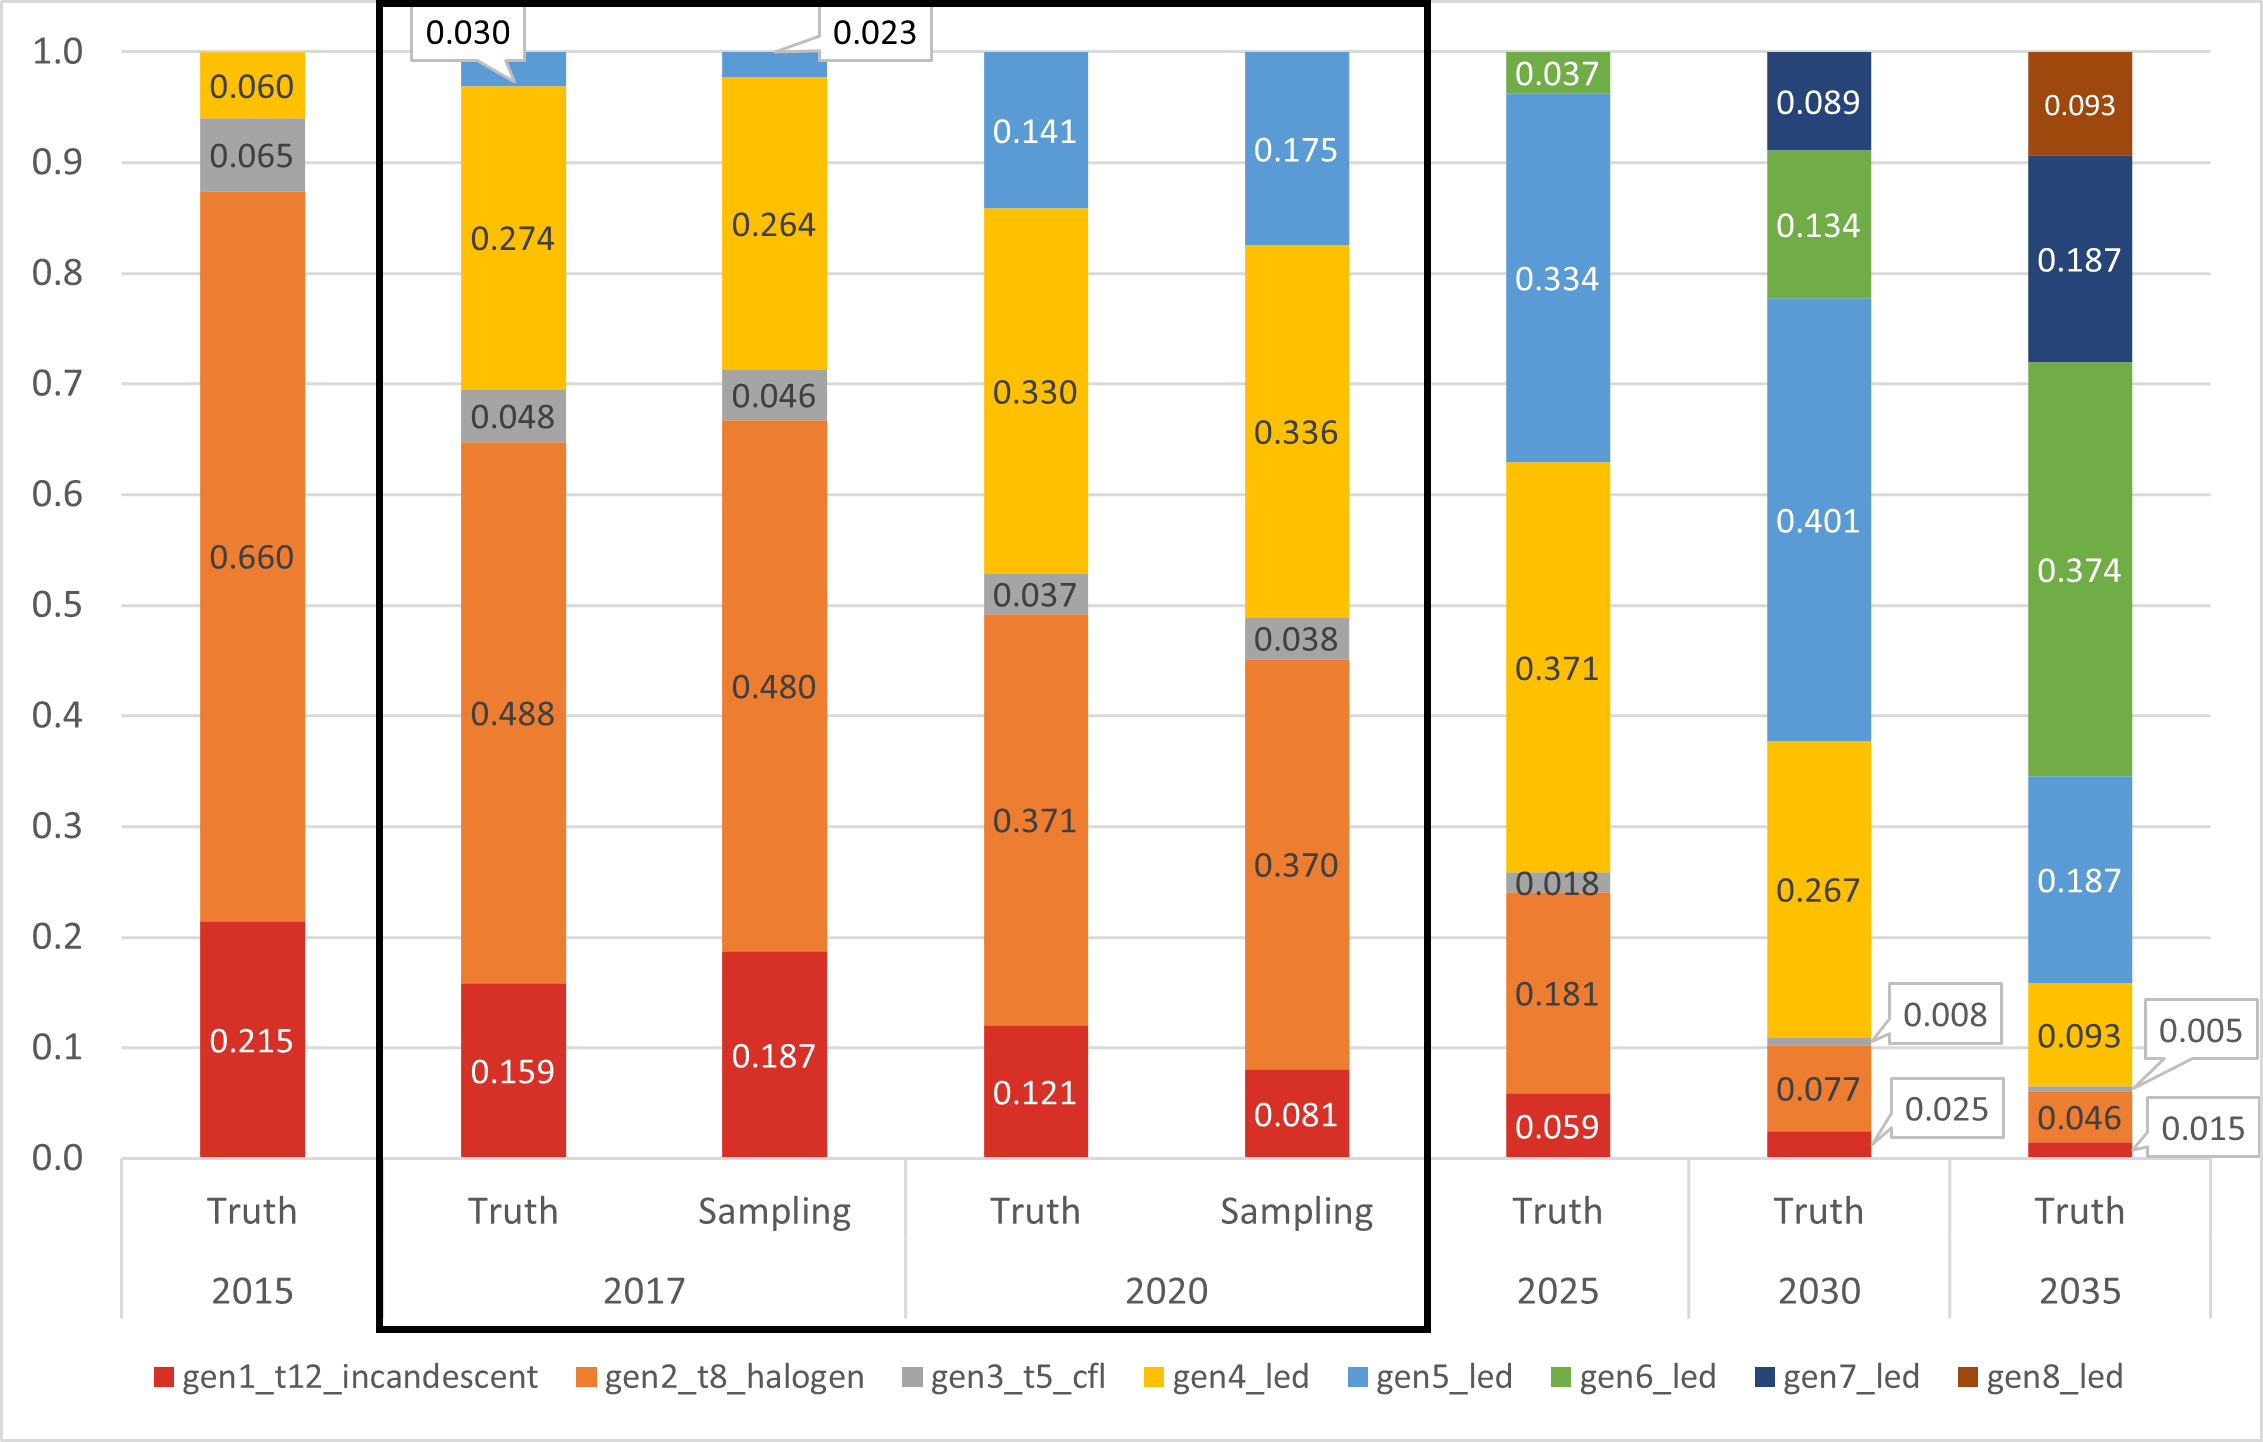
\includegraphics[width=0.8\textwidth]{figures/ltg_truth_vs_sampling.png}
    \caption[Interior lighting generation distributions]{``Truth'' lighting generation distribution data from \cite{doe2015lmc} and \cite{doe2019ssl}, and comparison of 2017 and 2020 ComStock sampling results.}
    \label{fig:ltg_compare_dist}
\end{figure}

Simulation years 2017 and 2020 were the focus of validation because they represent the range of simulation years typically run for ComStock. Additionally, for a given iteration of the lighting generation distributions, the comparison results were inconsistent across simulation years. For example, for a set of lighting generation distributions that showed close comparisons for 2017 and 2020, years 2025--2035 were significantly different compared to the other future projections.  With improvements to the script that produces the distributions, close comparisons across all simulation years should be feasible.

Table \ref{tab:ltg_gen_tsv} provides a snapshot of the final probability distributions, which show a gradual shift to higher generations as the year of the last interior lighting replacement increases. For this code year (ComStock 90.1-2013), generation 1 lighting technologies would likely not be installed. This is reflected in the distributions, as the minimum lighting generation installed is at least generation 2.  The relative popularity of each generation is also apparent in the distributions: generation 2 has a much higher probability of being installed in any year than generation 3, a less popular technology set.

%\begin{table}
\scriptsize
\centering
\caption{Interior Lighting Generation Distributions for ComStock 90.1-2013 Code Year}
\label{tab:ltg_gen_tsv}
\begin{tabular}{|l|l|l|l|l|l|l|l|l|l|}
\hline
\textbf{Energy Code}        & \textbf{Yea}r      & \textbf{gen1\_t12\_incandescent} & \textbf{gen2\_t8\_halogen} & \textbf{gen3\_t5\_cfl} & \textbf{gen4\_led} & \textbf{gen5\_led} & \textbf{gen6\_led} & \textbf{gen7\_led} & \textbf{gen8\_led} \\ \hline
ComStock 90.1-2013 & pre\_1978 & 0 & 1     & 0     & 0         & 0        & 0        & 0        & 0        \\ \hline
ComStock 90.1-2013 & 1978      & 0 & 1     & 0     & 0         & 0        & 0        & 0        & 0        \\ \hline
ComStock 90.1-2013 & 1979      & 0 & 1     & 0     & 0         & 0        & 0        & 0        & 0        \\ \hline
ComStock 90.1-2013 & 1980      & 0 & 1     & 0     & 0         & 0        & 0        & 0        & 0        \\ \hline
ComStock 90.1-2013 & 1981      & 0 & 1     & 0     & 0         & 0        & 0        & 0        & 0        \\ \hline
ComStock 90.1-2013 & 1982      & 0 & 1     & 0     & 0         & 0        & 0        & 0        & 0        \\ \hline
ComStock 90.1-2013 & 1983      & 0 & 1     & 0     & 0         & 0        & 0        & 0        & 0        \\ \hline
ComStock 90.1-2013 & 1984      & 0 & 1     & 0     & 0         & 0        & 0        & 0        & 0        \\ \hline
ComStock 90.1-2013 & 1985      & 0 & 1     & 0     & 0         & 0        & 0        & 0        & 0        \\ \hline
ComStock 90.1-2013 & 1986      & 0 & 1     & 0     & 0         & 0        & 0        & 0        & 0        \\ \hline
ComStock 90.1-2013 & 1987      & 0 & 1     & 0     & 0         & 0        & 0        & 0        & 0        \\ \hline
ComStock 90.1-2013 & 1988      & 0 & 1     & 0     & 0         & 0        & 0        & 0        & 0        \\ \hline
ComStock 90.1-2013 & 1989      & 0 & 1     & 0     & 0         & 0        & 0        & 0        & 0        \\ \hline
ComStock 90.1-2013 & 1990      & 0 & 1     & 0     & 0         & 0        & 0        & 0        & 0        \\ \hline
ComStock 90.1-2013 & 1991      & 0 & 1     & 0     & 0         & 0        & 0        & 0        & 0        \\ \hline
ComStock 90.1-2013 & 1992      & 0 & 1     & 0     & 0         & 0        & 0        & 0        & 0        \\ \hline
ComStock 90.1-2013 & 1993      & 0 & 1     & 0     & 0         & 0        & 0        & 0        & 0        \\ \hline
ComStock 90.1-2013 & 1994      & 0 & 1     & 0     & 0         & 0        & 0        & 0        & 0        \\ \hline
ComStock 90.1-2013 & 1995      & 0 & 0.990 & 0.010 & 0         & 0        & 0        & 0        & 0        \\ \hline
ComStock 90.1-2013 & 1996      & 0 & 0.983 & 0.017 & 0         & 0        & 0        & 0        & 0        \\ \hline
ComStock 90.1-2013 & 1997      & 0 & 0.992 & 0.008 & 0         & 0        & 0        & 0        & 0        \\ \hline
ComStock 90.1-2013 & 1998      & 0 & 0.985 & 0.015 & 0         & 0        & 0        & 0        & 0        \\ \hline
ComStock 90.1-2013 & 1999      & 0 & 0.987 & 0.013 & 0         & 0        & 0        & 0        & 0        \\ \hline
ComStock 90.1-2013 & 2000      & 0 & 0.973 & 0.027 & 0         & 0        & 0        & 0        & 0        \\ \hline
ComStock 90.1-2013 & 2001      & 0 & 0.981 & 0.019 & 0         & 0        & 0        & 0        & 0        \\ \hline
ComStock 90.1-2013 & 2002      & 0 & 0.967 & 0.033 & 0         & 0        & 0        & 0        & 0        \\ \hline
ComStock 90.1-2013 & 2003      & 0 & 0.966 & 0.034 & 0         & 0        & 0        & 0        & 0        \\ \hline
ComStock 90.1-2013 & 2004      & 0 & 0.964 & 0.036 & 0         & 0        & 0        & 0        & 0        \\ \hline
ComStock 90.1-2013 & 2005      & 0 & 0.911 & 0.040 & 0.049     & 0        & 0        & 0        & 0        \\ \hline
ComStock 90.1-2013 & 2006      & 0 & 0.910 & 0.049 & 0.041     & 0        & 0        & 0        & 0        \\ \hline
ComStock 90.1-2013 & 2007      & 0 & 0.887 & 0.050 & 0.062     & 0        & 0        & 0        & 0        \\ \hline
ComStock 90.1-2013 & 2008      & 0 & 0.826 & 0.058 & 0.115     & 0        & 0        & 0        & 0        \\ \hline
ComStock 90.1-2013 & 2009      & 0 & 0.810 & 0.047 & 0.143     & 0        & 0        & 0        & 0        \\ \hline
ComStock 90.1-2013 & 2010      & 0 & 0.782 & 0.050 & 0.168     & 0        & 0        & 0        & 0        \\ \hline
ComStock 90.1-2013 & 2011      & 0 & 0.738 & 0.055 & 0.207     & 0        & 0        & 0        & 0        \\ \hline
ComStock 90.1-2013 & 2012      & 0 & 0.598 & 0.055 & 0.348     & 0        & 0        & 0        & 0        \\ \hline
ComStock 90.1-2013 & 2013      & 0 & 0.670 & 0.043 & 0.287     & 0        & 0        & 0        & 0        \\ \hline
ComStock 90.1-2013 & 2014      & 0 & 0.568 & 0.055 & 0.377     & 0        & 0        & 0        & 0        \\ \hline
ComStock 90.1-2013 & 2015      & 0 & 0.553 & 0.059 & 0.387     & 0        & 0        & 0        & 0        \\ \hline
ComStock 90.1-2013 & 2016      & 0 & 0.519 & 0.051 & 0.430     & 0        & 0        & 0        & 0        \\ \hline
ComStock 90.1-2013 & 2017      & 0 & 0.413 & 0.042 & 0.313     & 0.231    & 0        & 0        & 0        \\ \hline
ComStock 90.1-2013 & 2018      & 0 & 0.241 & 0.031 & 0.345     & 0.382    & 0        & 0        & 0        \\ \hline
ComStock 90.1-2013 & 2019      & 0 & 0.191 & 0.022 & 0.264     & 0.523    & 0        & 0        & 0        \\ \hline
ComStock 90.1-2013 & 2020      & 0 & 0.195 & 0.022 & 0.311     & 0.472    & 0        & 0        & 0        \\ \hline
ComStock 90.1-2013 & 2021      & 0 & 0.146 & 0.011 & 0.196     & 0.551    & 0.096    & 0        & 0        \\ \hline
ComStock 90.1-2013 & 2022      & 0 & 0.107 & 0.009 & 0.168     & 0.612    & 0.104    & 0        & 0        \\ \hline
ComStock 90.1-2013 & 2023      & 0 & 0.058 & 0.006 & 0.116     & 0.738    & 0.082    & 0        & 0        \\ \hline
ComStock 90.1-2013 & 2024      & 0 & 0.049 & 0.004 & 0.100     & 0.689    & 0.157    & 0        & 0        \\ \hline
ComStock 90.1-2013 & 2025      & 0 & 0.037 & 0.003 & 0.069     & 0.695    & 0.195    & 0        & 0        \\ \hline
ComStock 90.1-2013 & 2026      & 0 & 0.025 & 0.002 & 0.061     & 0.691    & 0.154    & 0.067    & 0        \\ \hline
ComStock 90.1-2013 & 2027      & 0 & 0.017 & 0.002 & 0.043     & 0.594    & 0.213    & 0.131    & 0        \\ \hline
ComStock 90.1-2013 & 2028      & 0 & 0.013 & 0.002 & 0.035     & 0.615    & 0.195    & 0.140    & 0        \\ \hline
ComStock 90.1-2013 & 2029      & 0 & 0.011 & 0.001 & 0.024     & 0.463    & 0.236    & 0.264    & 0        \\ \hline
ComStock 90.1-2013 & 2030      & 0 & 0.007 & 0.001 & 0.017     & 0.396    & 0.220    & 0.360    & 0        \\ \hline    
ComStock 90.1-2013 & 2031 & 0 & 0.00683  & 0.000283 & 0.012582 & 0.33231  & 0.167166 & 0.444878 & 0.03595  \\ \hline
ComStock 90.1-2013 & 2032 & 0 & 0.009644 & 0.000405 & 0.013502 & 0.286907 & 0.163947 & 0.409868 & 0.115727 \\ \hline
ComStock 90.1-2013 & 2033 & 0 & 0.004305 & 0.000171 & 0.009392 & 0.182943 & 0.142833 & 0.508719 & 0.151637 \\ \hline
ComStock 90.1-2013 & 2034 & 0 & 0.005903 & 0.000172 & 0.008657 & 0.175607 & 0.096412 & 0.408274 & 0.304976 \\ \hline
ComStock 90.1-2013 & 2035 & 0 & 0.002496 & 0.000182 & 0.005823 & 0.132581 & 0.089427 & 0.317155 & 0.452336 \\ \hline
ComStock 90.1-2013 & 2036 & 0 & 0.003223 & 0        & 0.006906 & 0.097836 & 0.069061 & 0.310773 & 0.512201 \\ \hline
ComStock 90.1-2013 & 2037 & 0 & 0.006475 & 0        & 0.005396 & 0.080264 & 0.051261 & 0.168623 & 0.687981 \\ \hline
ComStock 90.1-2013 & 2038 & 0 & 0.005624 & 0        & 0.005624 & 0.07683  & 0.068294 & 0.130561 & 0.713066 \\ \hline
ComStock 90.1-2013 & 2039 & 0 & 0.004154 & 0        & 0.004154 & 0.088266 & 0.046729 & 0.116822 & 0.739875 \\ \hline
ComStock 90.1-2013 & 2040 & 0 & 0.006483 & 0        & 0.004862 & 0.068882 & 0.008104 & 0.060778 & 0.850891 \\ \hline
ComStock 90.1-2013 & 2041 & 0 & 0        & 0        & 0        & 0        & 0        & 0        & 1        \\ \hline
ComStock 90.1-2013 & 2042 & 0 & 0        & 0        & 0        & 0        & 0        & 0        & 1        \\ \hline
ComStock 90.1-2013 & 2043 & 0 & 0        & 0        & 0        & 0        & 0        & 0        & 1        \\ \hline

\end{tabular}
\end{table}

\pagebreak

There are two primary areas for improvement for this process:
\begin{itemize}
\item The first is in the initial Gaussian distributions. Although there is good data about when the lighting generations were first installed and when they finally lost popularity, information about when the generations peaked in their install popularity is not available. The current method assumes that the peak is at the midpoint of the start and end year. This is most likely incorrect. If data on the peak year of each generation could be collected, this would improve the distribution generation process.
\item The second improvement area is the final weighting process. The weights are currently determined using a guess-and-check method.  Further improvements to the distribution script would make this method more robust (e.g., using an optimization algorithm).
\end{itemize}

Figure \ref{fig:ltg_size_dist} shows the breakdown of lighting generation distribution (by count) by building size for 2018, the year the current ComStock data set represents the United States building stock. Small buildings are under 50,000 ft$^2$ and are assumed to have slower retrofit frequency than larger buildings (>50,000 ft$^2$). The data trend matches this assumption, as there is a larger percentage of smaller building models that have generation 1 and 2 lighting technologies.

Figure \ref{fig:ltg_btype_dist} provides a breakdown of lighting generation distributions by building type. There is not huge variation among the building types. However, building types that are typically smaller (quick service restaurants, small offices, strip malls) lag behind the other building types in terms of lighting technology.  This is consistent with the data in Figure \ref{fig:ltg_size_dist}.

\begin{figure}[ht!]
    \centering 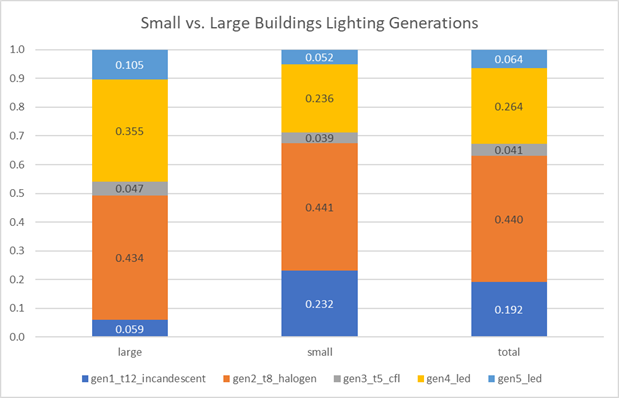
\includegraphics[width=0.8\textwidth]{figures/ltg_size_dist.png}
    \caption[Fraction of installed lighting generations by building size] {Fraction of installed lighting generations by building size (count-based distribution).}
    \label{fig:ltg_size_dist}
\end{figure}

\begin{figure}[ht!]
    \centering 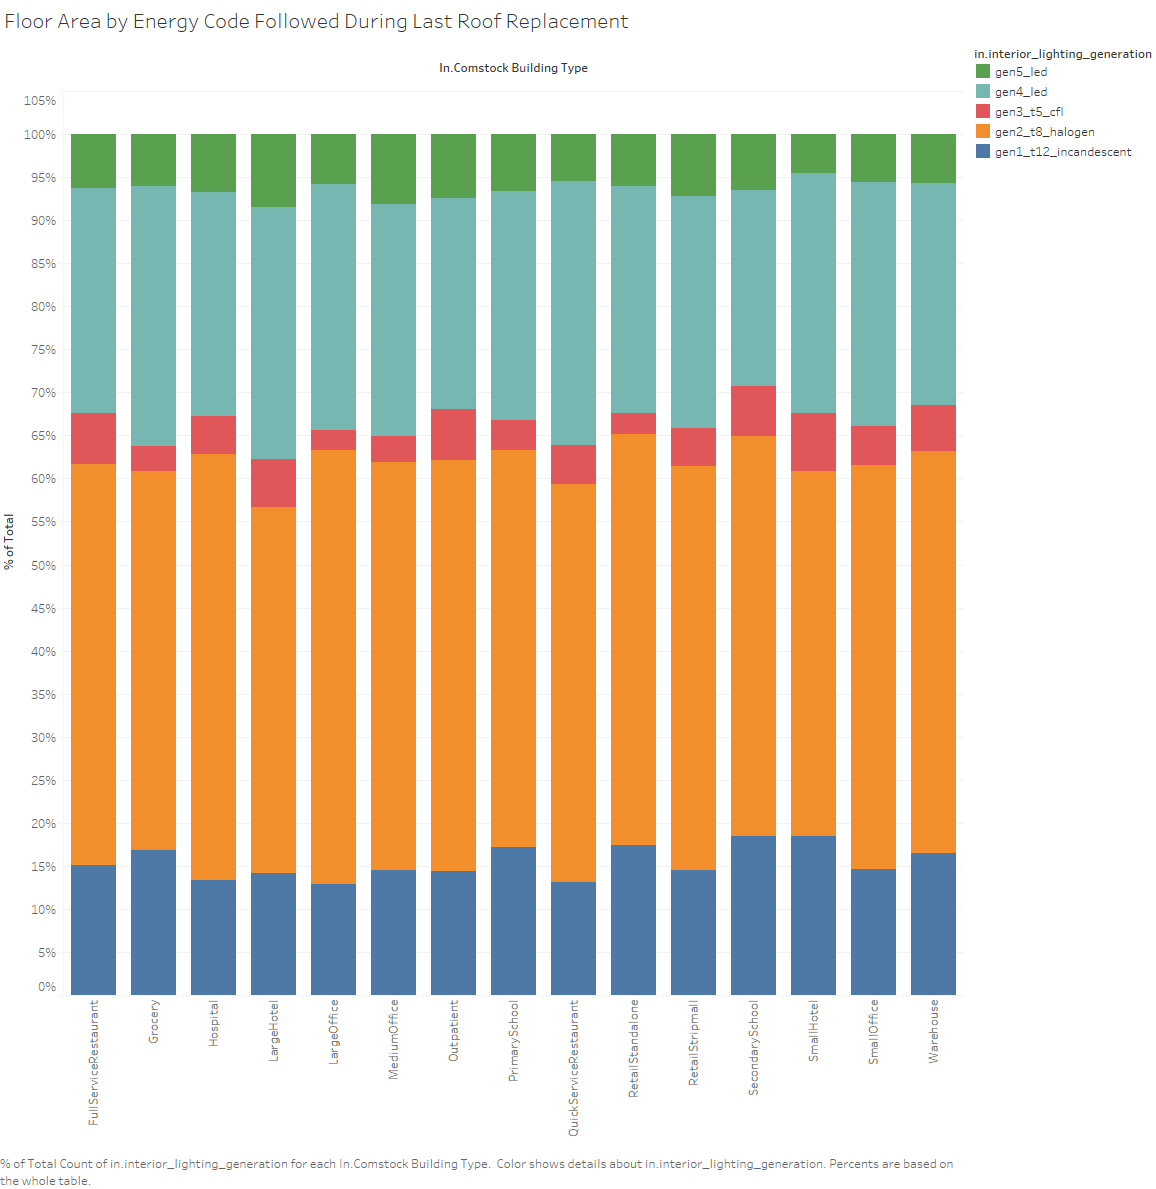
\includegraphics[width=0.9\textwidth]{figures/ltg_btype_dist.png}
    \caption[Fraction of installed lighting generation by building type]{Fraction of installed lighting generation by building type (count-based distribution).}
    \label{fig:ltg_btype_dist}
\end{figure}

\pagebreak

\subsubsection{Default Interior Lighting Schedules}
Default interior lighting schedules come from the openstudio-standards DOE prototype building models \citep{deru_2011}.  The End-Use Load Profiles project derived new default lighting schedules for restaurant, retail, education, office, and warehouse buildings, detailed in Section 3.3.1 of the EULP report: ``Interior Lighting Schedules'' \citep{eulp_method_2022}. A full list of default ComStock schedules is available as a  \href{https://github.com/NREL/openstudio-standards/blob/master/lib/openstudio-standards/standards/ashrae_90_1/ashrae_90_1_2013/comstock_ashrae_90_1_2013/data/ashrae_90_1.schedules.json}{schedules .json file} on the openstudio-standards GitHub repository.

Additional changes to default schedules include:

\begin{itemize}
  \item The peak lighting value in the end-use data derived hourly schedule for office spaces is now 0.85 instead of the original ~0.5.
  \item Quick service restaurants and kitchens use the FoodService\_Restaurant BLDG\_LIGHT\_EndUseData schedule rather than the prototype schedule.
  \item All large hotel guest room lighting schedules use HotelLarge BLDG\_LIGHT\_GUESTROOM\_SCH\_2013.
  \item All small hotel guest rooms follow the same default lighting schedule, with the midday lighting fraction changed from the prototype schedule value of ~0.3 to 0.15. Vacant guest rooms use an always off lighting schedule.
\end{itemize}

Interior lighting schedules are adjusted to correspond with the building's operating hours, as described in Section \ref{sec:hoo}.

\subsubsection{Interior Lighting Schedule Magnitude Variability}
Section 3.3.4 in the End-Use Load Profiles project report, ``Interior Lighting Schedule Magnitude Variability'' \citep{eulp_method_2022}, details the derivation of base-to-peak values applied to the default lighting schedules.

Figure \ref{fig:ltg_bpr} shows the distribution of base-to-peak ratios (BPRs) in the stock by building type for weekdays and weekends.  Note that this methodology was not applied to hospital, outpatient, small and large hotel, and warehouse building types, due to a lack of data.

\begin{figure}
    \centering 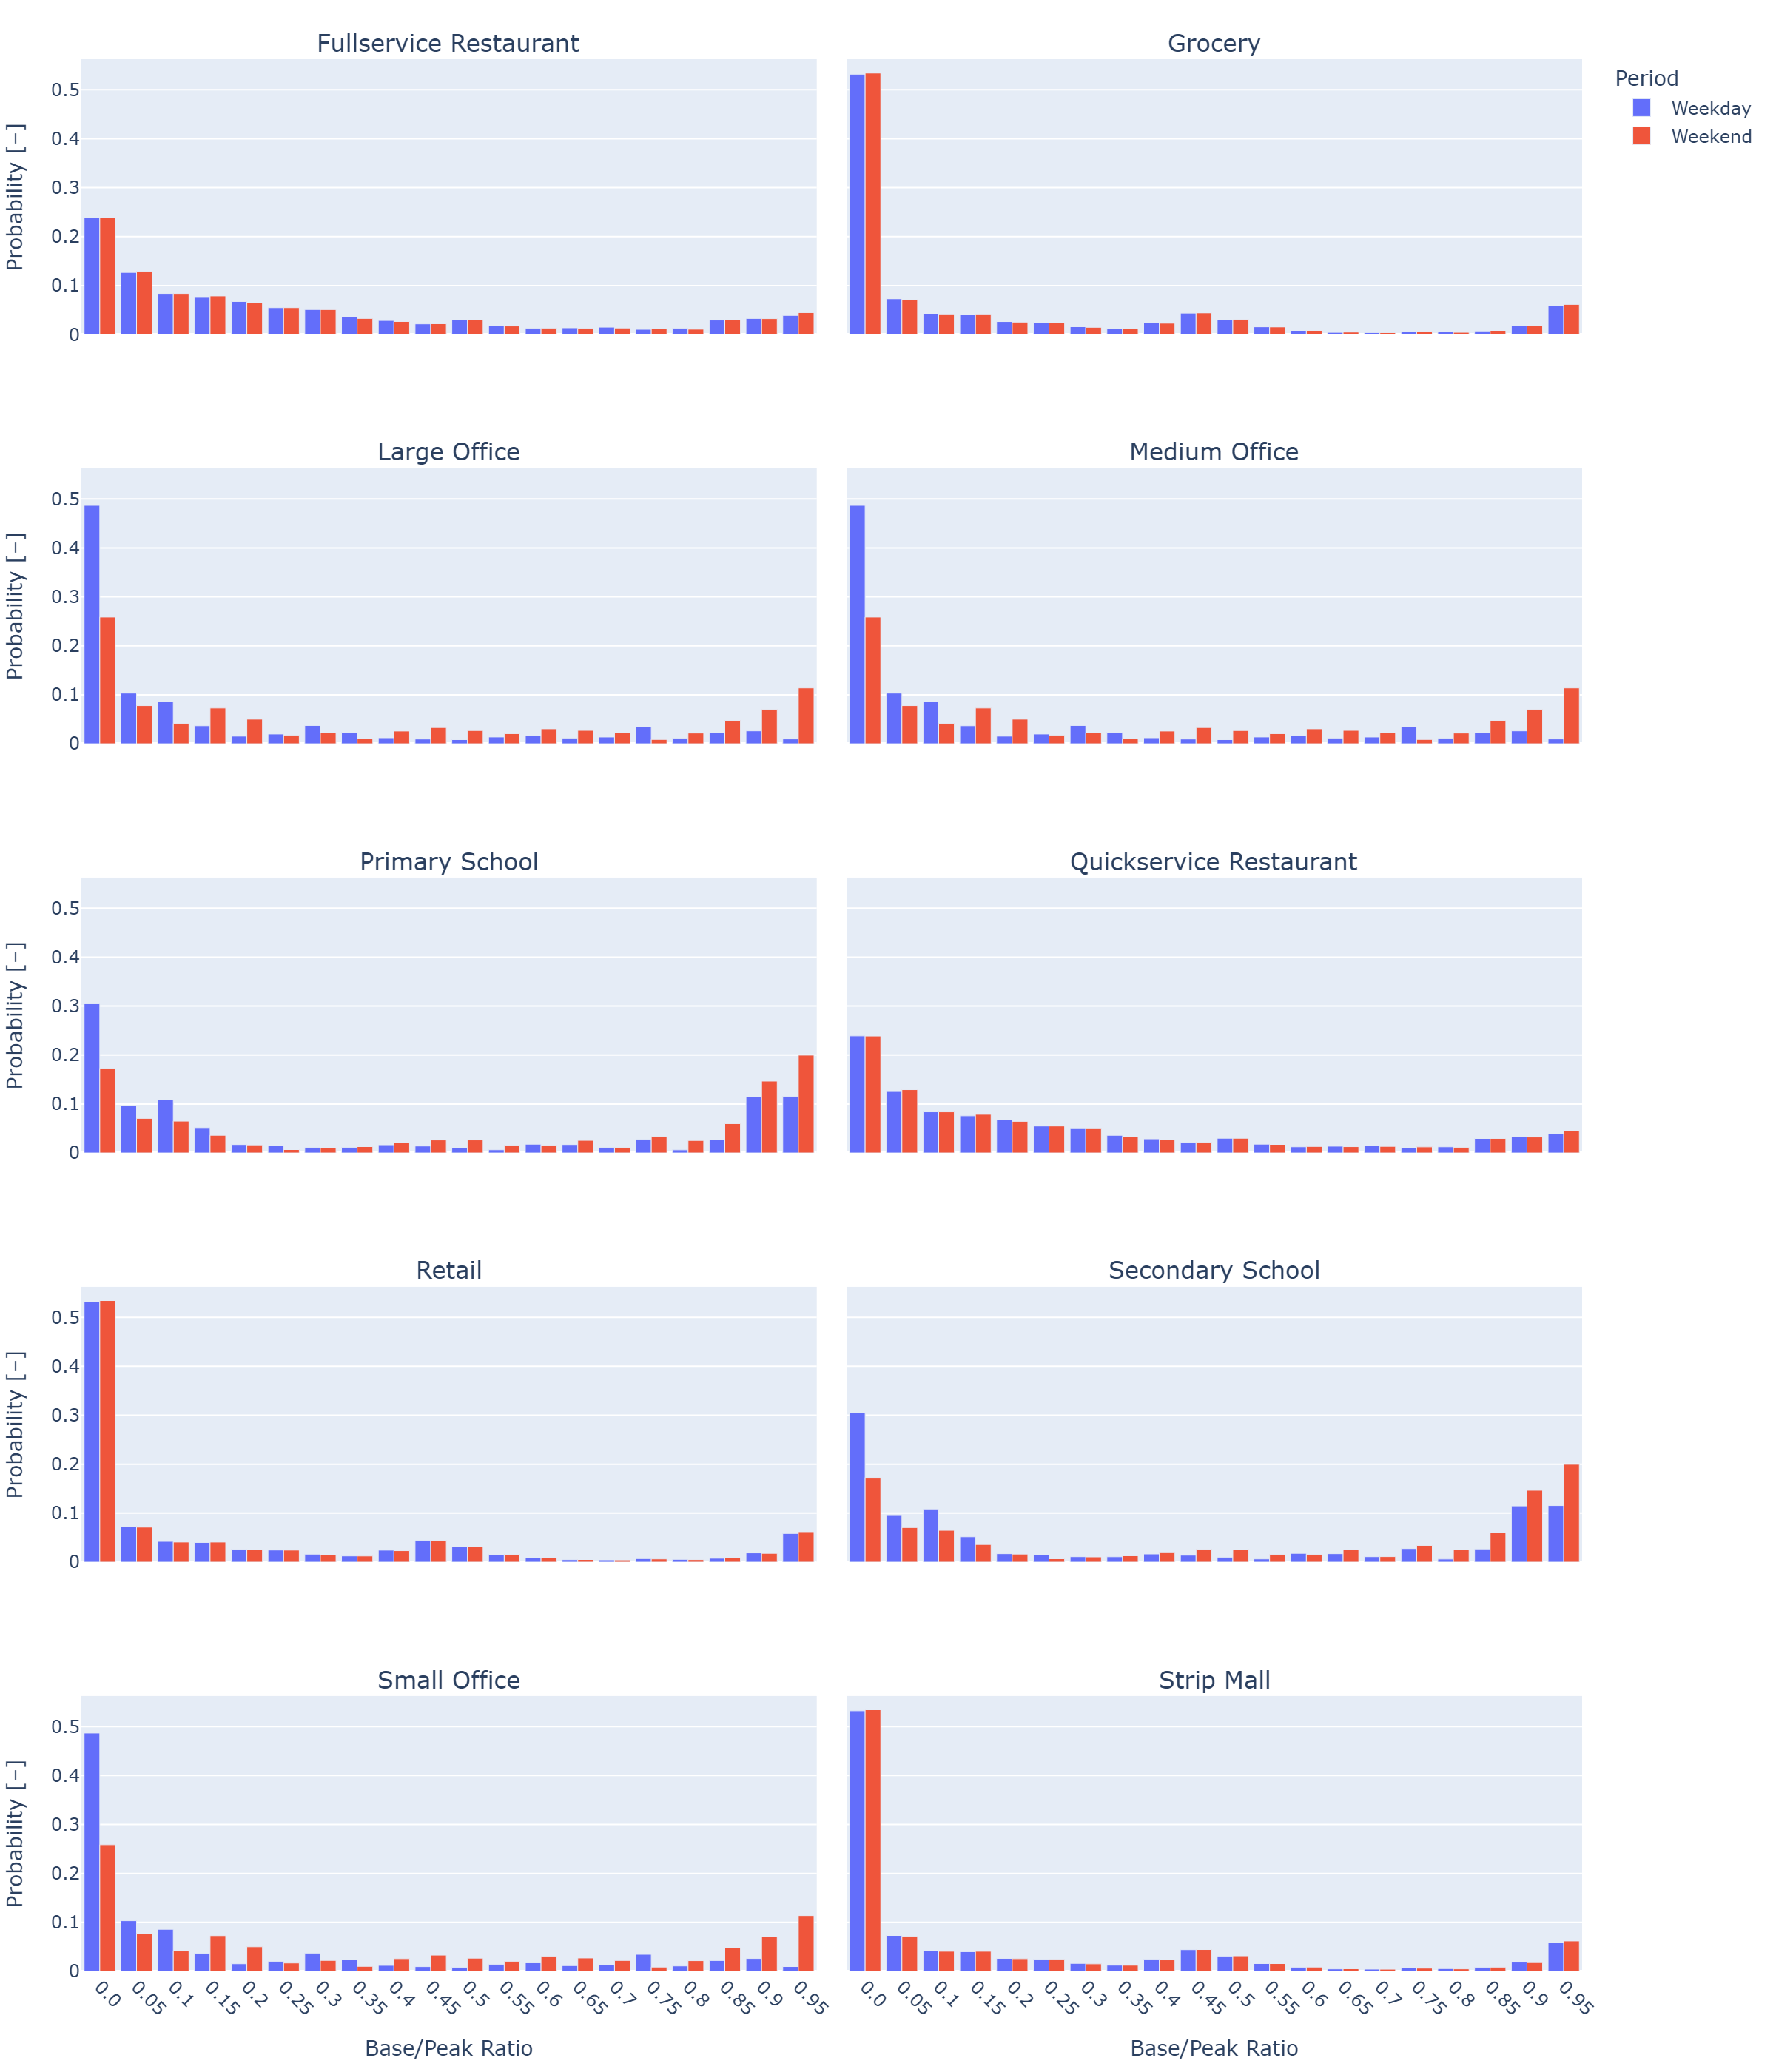
\includegraphics[width=0.9\textwidth]{figures/ltg_sch_bpr.png}
    \caption[Weekday and weekend lighting base-to-peak ratios by building type]{Weekday and weekend lighting base-to-peak ratios by building type. Base-to-peak ratio is on the x-axis, and fraction of the stock is on the y-axis.}
    \label{fig:ltg_bpr}
\end{figure}

\begin{figure}
    \centering 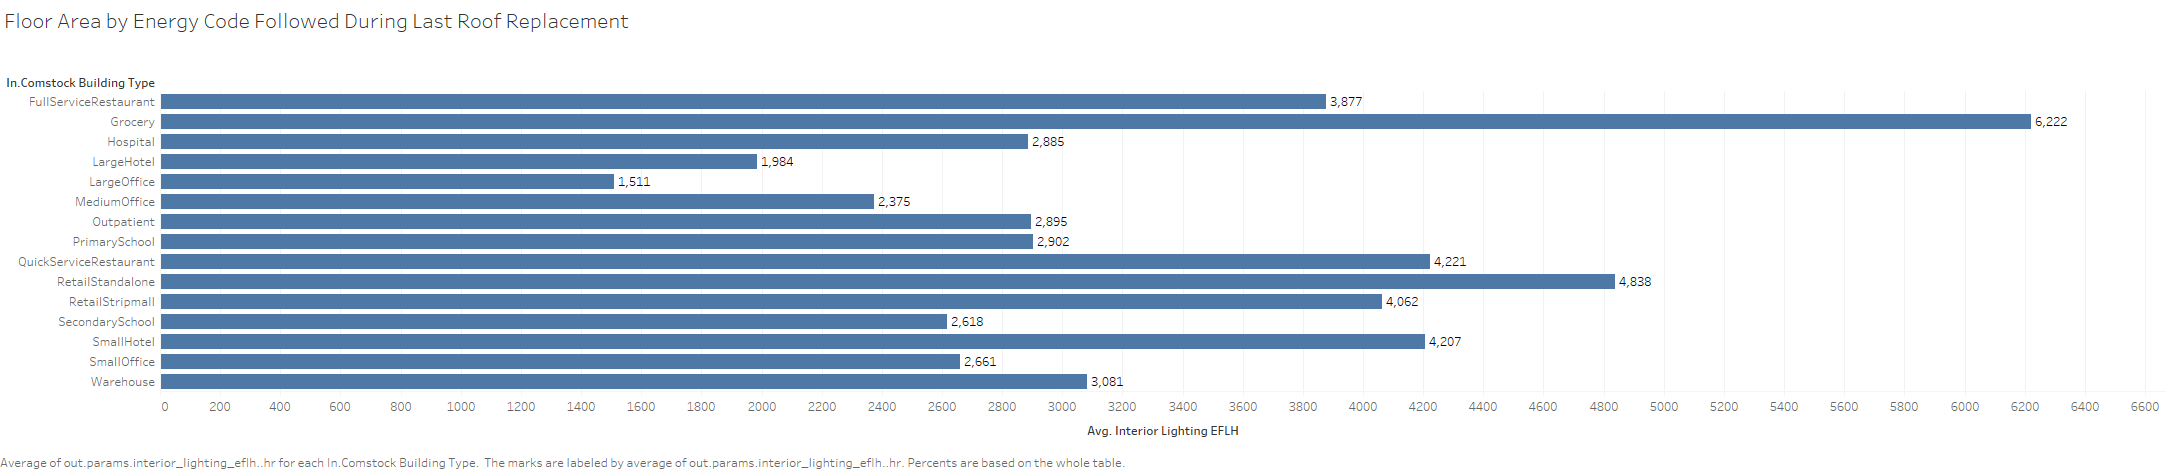
\includegraphics[width=1.0\textwidth]{figures/interior_lighting_eflh.png}
    \caption[Average interior lighting equivalent full load hours by building type]{Average interior lighting equivalent full load hours by building type.}
    \label{fig:interior_lighting_eflh}
\end{figure}

\subsection{Exterior Lighting}
Exterior lighting is all outdoor lighting at the building site, including lighting for parking, walkways, doorways, canopies, building facades, signage, and landscaping.

\subsubsection{Parking Area Lighting}
Parking area lighting accounts for the majority of exterior lighting in the stock \citep{doe2015lmc}. Parking lighting is calculated as the parking area times the installed lighting power per unit of parking area. Parking area is based on the estimated number of parking spots per student for schools, per unit for hotels, per bed for hospitals, and per building floor area for all other building types.  Parking spots are assumed to be 405 ft$^2$. Table \ref{tab:parking} details these assumptions.

%\begin{table}
\small
\centering
\caption[Parking]{Parking; Values From \cite{osti_1015277} Table 4.17}
\label{tab:parking}
\begin{tabular}{|l|p{0.75in}|p{0.5in}|p{0.5in}|p{0.5in}|p{0.75in}|p{1.5in}|}
\hline
\textbf{Building Type} & \textbf{Building Area Per Spot (ft$^2$)} & \textbf{Units Per Spot} & \textbf{Students Per Spot} & \textbf{Beds Per Spot} & \textbf{Parking Area Per Spot (ft$^2$)} \\ \hline
SmallOffice & 250 & & & & 405 \\ \hline
MediumOffice & 250 & & & & 405  \\ \hline
LargeOffice & 620 & & & & 405  \\ \hline
Retail & 285.7 & & & & 405  \\ \hline
StripMall & 215 & & & & 405  \\ \hline
PrimarySchool & & & 17 & & 405 \\ \hline
SecondarySchool & & & 8 & & 405 \\ \hline
Outpatient & 200 & & & & 405 \\ \hline
Hospital & & & & 0.83 & 405 \\ \hline
SmallHotel & & 1 & & & 405 \\ \hline
LargeHotel & & 1 & & & 405 \\ \hline
Warehouse & 1,000 & & & & 405 \\ \hline
QuickServiceRestaurant & 100 & & & & 405 \\ \hline
FullServiceRestaurant & 100 & & & & 405 \\ \hline
\end{tabular}
\end{table}

Lighting power for a given parking area is determined from the 2015 U.S. Lighting Market Characterization report, which assumes an average of 216 Watts (W) per parking lighting system, or 0.0410 W/ft\textsuperscript{2} (per equation \ref{ext_light_eqn}). Base parking lighting power allowance values for each vintage were reduced by a calculated factor such that the building-count weighted parking lighting power density came out to the 0.0410 W/ft\textsuperscript{2} target.  Note that this calculation is from 2015, so it overestimates the amount of exterior lighting in the stock, which has been changing over to use LEDs. The values for each vintage are shown in Table~\ref{tab:exterior_lighting_power}.

\begin{align}
\label{ext_light_eqn}
LPD = \left(\frac{216\,W}{\text{lighting system}}\right) \cdot \left(\frac{1\,\text{lighting system}}{13\,\text{parking spots}}\right) \cdot \left(\frac{1\,\text{parking spot}}{405\,\text{ft}^2}\right) = 0.0410\,W/\text{ft}^2
\end{align}

%\begin{table}
\centering
\scriptsize
\caption{Exterior Lighting Power}
\label{tab:exterior_lighting_power}
\begin{tabular}{|p{0.5in}|p{0.3in}|p{0.4in}|p{0.3in}|p{0.3in}|p{0.35in}|p{0.3in}|p{0.3in}|p{0.35in}|p{0.3in}|p{0.35in}|p{0.35in}|}
\hline
\textbf{Template} & \textbf{Building Facade and Landscape Automatic Shutoff} & \textbf{Occupancy Setback Reduction} & \textbf{Base Site Allowance Power (W)} & \textbf{Base Site Allowance Fraction} & \textbf{Parking Areas and Drives (W/ft\textsuperscript{2})} & \textbf{Main Entries (W/ft)} & \textbf{Other Doors (W/ft)} & \textbf{Entry Canopies (W/ft\textsuperscript{2})} & \textbf{Building Facades (W/ft\textsuperscript{2})} & \textbf{Loading Areas For Emergency Vehicles (W/ft\textsuperscript{2})} & \textbf{Drive Through Windows and Doors (W)}  \\
\hline
Pre-1980          & FALSE & 0   &                         & 0.05   & 0.18     & 30 & 25 & 10   & 0.25 & 4     & 400 \\ \hline
1980--2004         & FALSE & 0   &                         & 0.05   & 0.049749 & 30 & 25 & 1.5  & 0.25 & 4     & 400 \\ \hline
90.1-2004         & TRUE  & 0   &                         & 0.05   & 0.041458 & 30 & 20 & 1.25 & 0.2  & 0.5   & 400 \\ \hline
90.1-2007         & TRUE  & 0   &                         & 0.05   & 0.041458 & 30 & 20 & 1.25 & 0.2  & 0.5   & 400 \\ \hline
90.1-2010         & TRUE  & 0.3 & 750                     &        & 0.027638 & 30 & 20 & 0.4  & 0.15 & 0.5   & 400 \\ \hline
90.1-2013         & TRUE  & 0.3 & 750                     &        & 0.027638 & 30 & 20 & 0.4  & 0.15 & 0.5   & 400 \\ \hline
90.1-2016         & TRUE  & 0.3 & 750                     &        & 0.027638 & 30 & 20 & 0.4  & 0.15 & 0.5   & 400 \\ \hline
90.1-2019         & TRUE  & 0.3 & 750                     &        & 0.027638 & 30 & 20 & 0.4  & 0.15 & 0.5   & 400 \\ \hline
DEER 1985         & FALSE & 0   &                         & 0.05   & 0.036491 & 30 & 25 & 1.5  & 0.25 & 4     & 400 \\ \hline
DEER 1996         & FALSE & 0   &                         & 0.05   & 0.036491 & 30 & 25 & 1.5  & 0.25 & 4     & 400 \\ \hline
DEER 2003         & TRUE  & 0   &                         & 0.05   & 0.036491 & 30 & 20 & 1.25 & 0.2  & 0.5   & 400 \\ \hline
DEER 2007         & TRUE  & 0   &                         & 0.05   & 0.036491 & 30 & 20 & 1.25 & 0.2  & 0.5   & 400 \\ \hline
DEER 2011         & TRUE  & 0.3 & 750                     &        & 0.036491 & 30 & 20 & 0.4  & 0.15 & 0.5   & 400 \\ \hline
DEER 2014         & TRUE  & 0.3 & 750                     &        & 0.018246 & 30 & 20 & 0.4  & 0.15 & 0.408 & 125 \\ \hline
DEER 2015         & TRUE  & 0.3 & 750                     &        & 0.018246 & 30 & 20 & 0.4  & 0.15 & 0.408 & 125 \\ \hline
DEER 2017         & TRUE  & 0.3 & 520                     &        & 0.018246 & 21 & 21 & 0.4  & 0.05 & 0.408 & 125 \\ \hline
\end{tabular}
\end{table}

\subsubsection{Other Exterior Lighting}
Non-parking exterior lighting is determined by the exterior lighting allowance specified in ASHRAE 90.1 for exterior lighting zone 3 (All Other Areas). Length and area estimates are determined from the values in Table \ref{tab:entryways}. The building facade area is calculated from the model as the ground floor exterior wall area. The lighting power allowance is matched to the 90.1 code for each vintage. The exterior lighting power allowances are shown in Table~\ref{tab:exterior_lighting_power}. Note that although 90.1 includes exterior lighting, the only forms of exterior lighting included in ComStock are parking areas, building facades, main entry doors, other doors, drive through windows, entry canopies, and emergency canopies. Notably, ComStock does not include lighting for exterior signage.

%\begin{table}
\small
\centering
\caption[Entryways]{Entryways; Values From \cite{osti_1015277} Table 4.18}
\label{tab:entryways}
% \begin{tabular}{|l|rp{1in}|p{1in}|p{1in}|p{1in}|p{1in}|p{1in}|p{1in}|}
\begin{tabular}{|l|p{1.5cm}|p{1.5cm}|p{1.5cm}|p{1.5cm}|p{1.75cm}|p{1.5cm}|p{1.5cm}|}
\hline
\textbf{Building Type} & \textbf{Rollup Doors (per 10,000 ft$^2$)} & \textbf{Entrance Doors (per 10,000 ft$^2$)} & \textbf{Other Doors (per 10,000 ft$^2$)} & \textbf{Entrance Canopies} & \textbf{Emergency Canopies} & \textbf{Canopy Size (ft$^2$)} & \textbf{Floor Area Per Drive Through Window (ft$^2$)} \\ \hline
SmallOffice            & 0.47 & 2 & 2     &   &   &      &      \\ \hline
MediumOffice           & 0.13 & 1 & 3     &   &   &      &      \\ \hline
LargeOffice            &      & 1 & 3     &   &   &      &      \\ \hline
Retail                 & 1.84 & 1 & 2.93  &   &   &      &      \\ \hline
StripMall              & 0.05 & 6 & 6.6   &   &   &      &      \\ \hline
PrimarySchool          & 0.07 & 2 & 3.3   &   &   &      &      \\ \hline
SecondarySchool        & 0.1  & 2 & 2.45  &   &   &      &      \\ \hline
Outpatient             & 0.1  & 1 & 5.19  &   &   &      &      \\ \hline
Hospital               & 0.03 & 2 & 3.8   &   & 1 & 720  &      \\ \hline
SmallHotel             &      & 2 & 28.91 & 1 &   & 720  &      \\ \hline
LargeHotel             &      & 2 & 2.27  & 1 &   & 1,620 &      \\ \hline
Warehouse              & 3.67 & 1 & 2     &   &   &      &      \\ \hline
QuickServiceRestaurant &      & 2 & 1     &   &   &      & 2,500 \\ \hline
FullServiceRestaurant  &      & 1 & 3     &   &   &      &      \\ \hline

\end{tabular}
\end{table}

\section{Plug and Process Loads}
\label{sec:plug_and_process_loads}

Plug and process loads (PPLs) are all electrical or gas building loads that do not fall under lighting, heating, cooling, ventilation, or water heating. As lighting and HVAC equipment becomes more efficient, PPLs represent an increasing percentage of commercial building energy consumption---up to 50\% in high-performance buildings. This section describes how electric equipment, gas equipment, data centers, elevators, and kitchen equipment are modeled in ComStock. 

\subsection{Electric Equipment}

Electric equipment is a broad category that encompasses any type of load that is powered by an AC outlet. This can include computers, monitors, printers, kitchen or bathroom appliances, laundry equipment, phone chargers, and more. Because there are so many types of electric equipment, ComStock does not model each technology separately, but instead uses an equipment power density (EPD) value for each space type, in watts per square foot. 

The EPDs are derived from the DOE prototype buildings; however, some of the values were adjusted during the end-use load profiles calibration process. Using end-use-level data provided by two industry sources for a variety of building types, we increased or decreased some EPD assumptions to better reflect the actual building data. Building types that were affected by the EPD adjustments included Full Services Restaurant (FullServiceRestaurant), Primary School (PrimarySchool), Quick Service Restaurant (QuickServiceRestaurant), Retail (Retail), Secondary School (SecondarySchool), and Strip Mall (StripMall). 

The EPDs are dependent on building type, space type, and DOE Reference Building template. The interior equipment template is a function of the vintage of the building, as well as equipment turnover assumptions. In most cases, the EPD remains constant for all templates; however, some values increase or decrease in newer templates. An increase in the EPD in newer templates for a particular space type most likely indicates that new types of plug loads or technologies are assumed to be in the space. By comparison, a decrease in EPD indicates that plug loads in that space have become more efficient as buildings upgrade to newer equipment. For example, EPDs in the ``MediumOffice - Conference'' space type decrease beginning with the 90.1-2004 template, reflecting an assumption that conference equipment such as projectors and monitors have become more efficient. On the other hand, EPDs in ``MediumOffice - Breakroom'' increase drastically, likely due to the addition of new kitchen appliances and accessories. 

The EPDs in the ComStock model for each combination of building type, space type, and template are shown in Table ~\ref{tab:epds}.


\subsection{Gas Equipment}

Gas equipment refers to any natural gas-powered interior equipment that is not used for space heating or water heating. Similar to electric equipment, there are many different types of gas equipment, so ComStock does not model each technology individually, but rather uses a gas intensity in BTU per hour per square foot. Gas kitchen equipment makes up the majority of the gas equipment modeled in ComStock. Kitchen equipment will be discussed separately in Section 4.6.5. There are only three non-kitchen space types in our models that contain non-zero gas equipment values, and the values used are shown in Table~\ref{tab:gas_equip}. 

\begin{table}
\small
\centering
\caption[Gas Equipment Power Density]{Gas Equipment Power Density (Btu/hr*ft\textsuperscript{2})}
\label{tab:gas_equip}
\begin{tabular}{|l|l|r|r|r|r|r|r|}
\hline
\multicolumn{2}{|c|}{} & \multicolumn{6}{c|}{{\textbf{Template}}} \\ \hline
\textbf{Building Type} & \textbf{Space Type} & \textbf{Pre-1980} & \textbf{1980--2004} & \textbf{90.1-2004} & \textbf{90.1-2007} & \textbf{90.1-2010} & \textbf{90.1-2013} \\ \hline
LargeHotel & Laundry  & 170.0 & 170.0 & 170.0 & 170.0 & 170.0 & 170.0 \\ \hline
Outpatient & OR      & 23.9 & 23.9 & 23.9 & 23.9 & 23.9 & 23.9 \\ \hline
SmallHotel & Laundry  & 58.4 & 58.4 & 129.9 & 129.9 & 129.9 & 129.9 \\ \hline
\end{tabular}
\end{table}

The space types that contain gas equipment are the laundry and operating room space types in hotels and outpatient buildings, respectively. Gas laundry equipment represents gas clothes dryers, which are common in commercial drying applications. In operating rooms, a small amount of gas equipment represents steam sterilizers or autoclaves, which are used for sterilization during surgical procedures.

\subsection{Data Centers}

Data centers are a high-intensity type of PPL that house IT and computing equipment. Large standalone data centers are not currently modeled in ComStock, but this building type may be added in the future. Instead, ComStock models data centers as a space type within large and medium office buildings. This is meant to represent an IT closet or high-performance computer that is located within an office building and used by a business or organization. 

The data center is divided into two space types---a core data center and an IT closet. The core data center represents about 96\% of the data center floor area and has an equipment power density of 45 W/ft\textsuperscript{2}. The IT closet represents the remaining 4\% of the data center floor area and has an equipment power density of 20 W/ft\textsuperscript{2}. The area-weighted equipment power density of the whole data center is 44 W/ft\textsuperscript{2}, which is approximately 20--50 times the equipment load of most other space types \citep{osti_1129366}.

In the DOE large office prototype model, the data center represents 2.5\% of the total floor area. The medium office prototype model does not contain a data center space type. If we used the exact space type ratios from the prototype models for ComStock, all large offices would contain a data center, but no medium or small offices would contain this space type. In reality, not all office buildings contain data centers, and they can be present in offices of different sizes. Therefore, ComStock models data centers in a portion of large and medium office buildings. To determine these distributions, we used CBECS 2012 data to understand how prevalent data centers are in office buildings of different sizes. In addition, we used CBECS responses to determine what percent of a typical office building's floor area is dedicated to the data center. From this analysis, we decided that 38\% of large offices and 20\% of medium offices should contain data centers. In buildings with data centers, that space should make up approximately 2\% of the total square footage of the building. We also determined that data centers are uncommon in small offices; therefore, there is no data center space type in the small office models. 

Data centers follow a very different schedule than the rest of a building's plug and process loads. This type of IT equipment often runs 24 hours a day; therefore, the data center space type has a constant schedule year round. The start and stop time and base-to-peak ratio (BPR) schedule adjustments do not affect the data center space type. 

\subsection{Elevators}
Elevators are a high power density equipment load present in many commercial buildings. According to the Americans with Disabilities Act (ADA), elevators are required in all commercial buildings with three or more stories, or when the square footage of each floor is more than 3,000 square feet. Although not a requirement, many two-story buildings also contain elevators for accessibility and convenience. Therefore, ComStock includes elevators in all buildings with two or more stories.

Hydraulic elevators are assumed to be installed in buildings with two to six stories, and traction elevators are assumed to be installed in buildings taller than six stories. Hydraulic elevators use a fluid-driven piston to lift the cab, and typically operate at speeds of 150 feet per minute or less. Hydraulic elevators are more affordable and can carry heavier loads, but because of their slow speeds, they are typically only used in buildings up to five stories. For buildings with six or more stories, traction elevators are used because they operate at much higher speeds (up to 500 feet per minute). Traction elevators use a counterweight and pulley system, making them more energy efficient because the motor does not have to move as much weight. The drawbacks, however, include high installation and maintenance costs and limits on cab weights. The motor power is assumed to be 16,055 W for hydraulic elevators and 20,370 W for traction elevators. 

Elevators are modeled as a zone load in EnergyPlus, meaning the elevator equipment load and associated heat gain are attributed to a thermal zone. Elevator load is reported out as part of the electric equipment end use. With hydraulic elevators, the elevator room is typically located in the basement, so the equipment load and heat gain are added to the first floor core zone. With traction elevators, the elevator equipment is located on the roof, so the equipment load and heat gain are added to the top floor core zone.

The number of elevators installed in a ComStock building depends on the building type. For most building types, the number of elevators is based on the floor area. The exceptions are hospitals and hospitality buildings, for which assumptions are based on the number of hospital beds or hotel rooms, respectively. ComStock differentiates between passenger elevators and freight elevators in order to properly capture the elevator load in certain building types with industrial or service elevators. Passenger elevators are modeled in all building types, whereas freight elevators are only modeled in hospital, large hotel, large office, and warehouse buildings. The assumptions for the number of passenger and freight elevators modeled by building type are shown in Tables ~\ref{tab:passenger_elevators} and ~\ref{tab:freight_elevators}.

The equipment schedule for elevators is irregular and unpredictable. Therefore, this load does not follow the typical plug load schedule for its associated space type. We decided to approximate an elevator's schedule by relating it to the number of people who are entering or exiting the building at each time step---in other words, the derivative of the occupancy schedule of the building. We also made assumptions regarding the number of people per elevator ride (five), the amount of time per ride (calculated from the elevator speed and number of stories), and the amount of inter-floor traffic that is not captured by the change in building occupancy (added a factor of 1.2x). Elevator data and metrics like this are not commonly measured or available, so these assumptions are based primarily on engineering judgment. 

From these calculations and assumptions, we derived an elevator schedule for each building type and each day of the week. An example of the elevator schedule for medium offices is shown in Figure~\ref{fig:medium_office_elevator_schedule} for weekdays, Saturdays, and Sundays. On weekdays, the most elevator traffic occurs at the beginning and end of the day, when people are coming in or leaving work for the day. There is also significant traffic during the lunch hour, as some people choose to leave the building for lunch. At all other times during the workday, the elevator load is approximately 40\% of the total load to account for inter-floor traffic and minimal change in the total building occupancy. For some buildings, the occupancy schedules are reduced on Saturdays and include no occupancy on Sundays, which is reflected in the elevator schedule. 

\begin{figure}[ht!]
    \centering 
    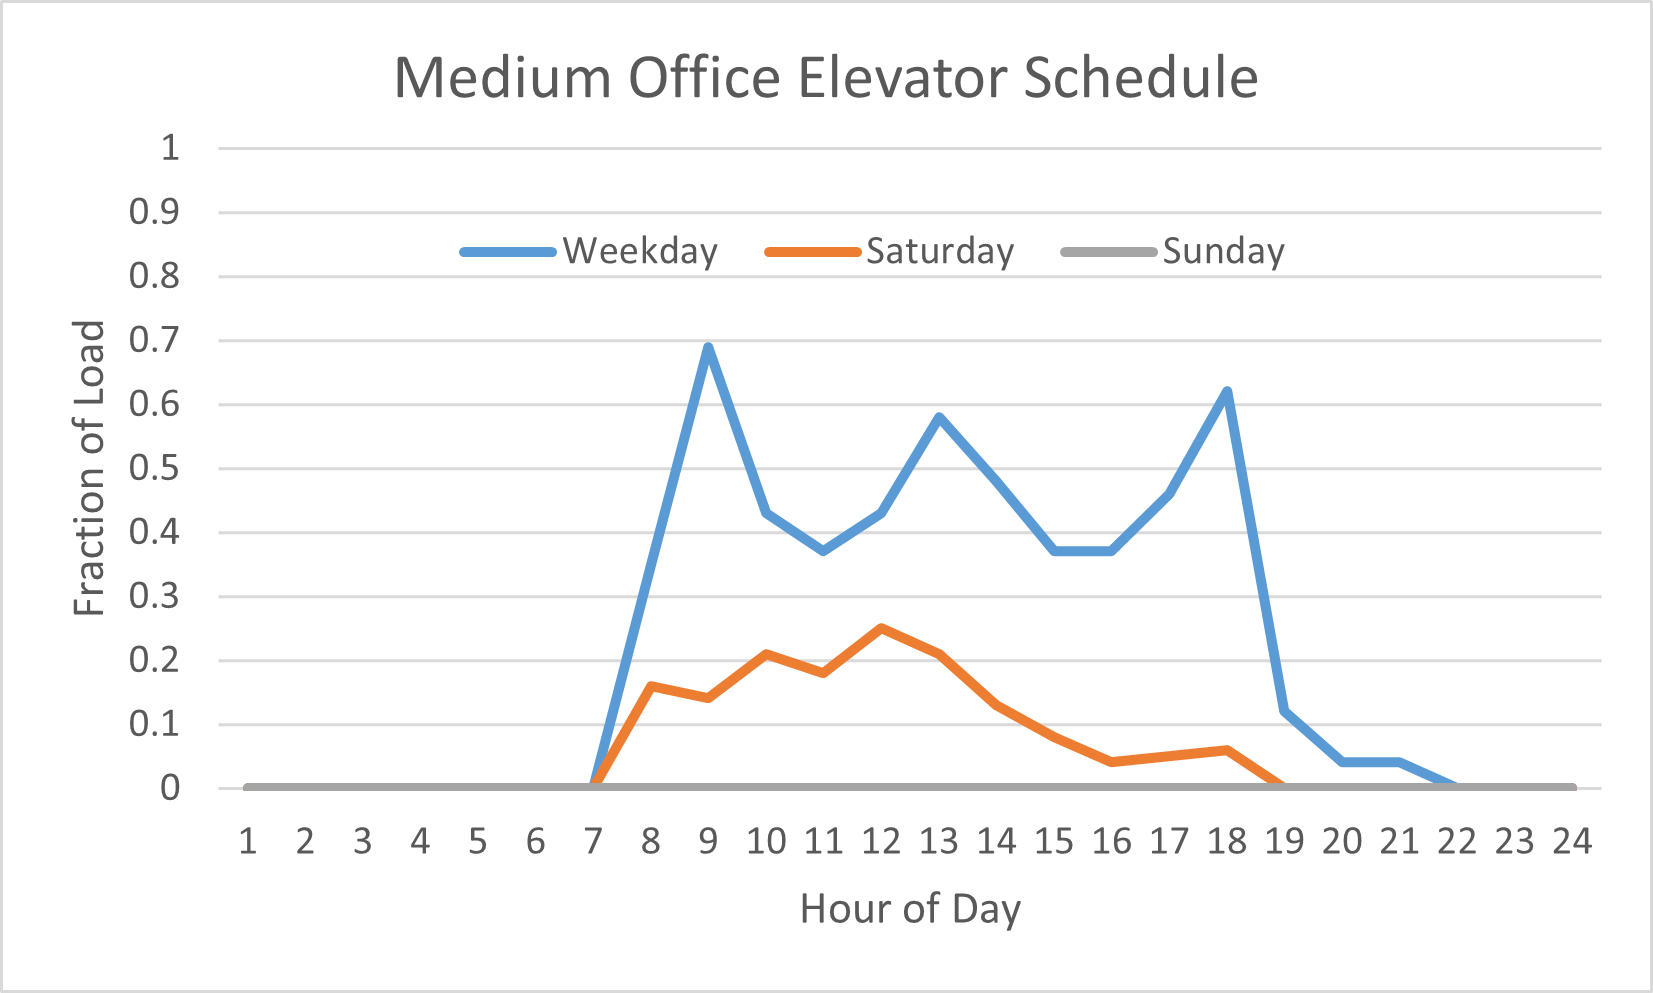
\includegraphics[]{figures/medium_office_elevator.png}
    \caption[Medium office elevator schedule]{Elevator fractional load schedule for medium offices on weekdays, Saturdays, and Sundays.}
    \label{fig:medium_office_elevator_schedule}
\end{figure}

The final aspect of modeling elevators is accounting for lighting and fans inside the elevator. Although these are minimal loads compared to the total elevator energy, they are still modeled in ComStock. The elevator lighting and fans are defined in the model by a total power in watts. These wattage values were calculated based on the number of elevators and the subsystem template in the model, thereby ensuring higher efficiencies for newer lighting and ventilation systems. The elevator lighting and fan schedules are assumed to be at full load at all times when the elevator schedule is greater than 0.

\pagebreak

\subsection{Kitchen Equipment} 
Kitchens are one of the most energy-intensive space types. In ComStock, kitchen space types are modeled in six building types---FullServiceRestaurant, Hospital, LargeHotel, PrimarySchool, QuickServiceRestaurant, and SecondarySchool. In some building types, namely restaurants, the kitchen space type represents a significant proportion of the floor area. In these cases, kitchen loads have a major impact on the total building EUI. In hotels, hospitals, and schools, the kitchen space type only represents a small fraction of the total floor area. Table~\ref{tab:kitchen_floor_area} shows the percent of the total floor area represented by the kitchen space type for each building type. Note that some of the strip malls in ComStock contain some fraction of the "QuickServiceRestaurant" building type to account for food service that is often found in strip malls. 

\begin{table}[h!]
\small
\centering
\caption[Kitchen Space Type Percentage of Total Floor Area]{Kitchen Space Type Percentage of Total Floor Area}
\label{tab:kitchen_floor_area}
\begin{tabular}{|l|l|l|}
\hline
\textbf{Building Type}          & \textbf{Space Type} & \textbf{Percentage of Total Floor Area} \\ \hline
FullServiceRestaurant  & Kitchen    & 27.3\%                         \\ \hline
Hospital               & Kitchen    & 4.1\%                          \\ \hline
LargeHotel             & Kitchen    & 0.9\%                          \\ \hline
PrimarySchool          & Kitchen    & 2.4\%                          \\ \hline
QuickServiceRestaurant & Kitchen    & 50\%                           \\ \hline
SecondarySchool        & Kitchen    & 1.1\%                          \\ \hline
\end{tabular}
\end{table}

Commercial building energy modeling often assumes an energy intensity per area for cooking equipment, like what is used in the DOE prototype buildings (\cite{qsr_50pct_svs}). However, applying these power densities directly to the various building sizes in ComStock assumes cooking loads scale linearly with kitchen square footage, which does not necessarily represent reality (\cite{eia2012cbecs},~\cite{qsr_50pct_svs}). Further, it does not allow for straightforward analysis of specific cooking equipment since it is represented by a single aggregate load. However, little information exists regarding representative equipment-specific modeling of cooking appliances, as well as how cooking equipment scales with building area. The CBECS survey does provide some level of guidance for area-based intensity as they disaggregate cooking energy consumption separately and provide building area for their samples, but this end use energy consumption data is derived using statistical means from monthly billing data rather than directly measured making it less reliable (\cite{eia2012cbecs},~\cite{qsr_50pct_svs}).


ComStock uses published data to create representative probability distributions of commercial cooking equipment counts, by building type, for both gas and electric appliances. Additionally, the equipment distributions are scaled by area to represent the non-linear scaling suggested in the literature. Although other building types likely include some degree of cooking equipment as well, such as larger offices (\cite{eia2012cbecs}), the current implementation of ComStock only includes cooking equipment in the previously-mentioned six building types plus quick service restaurants found in strip malls. 

Commercial kitchens can contain electric or gas cooking equipment, or a mix of both. The prevalence of gas and electric fuel types for each equipment type used in ComStock are derived from a DOE study (\cite{goetzler_commercial_appliances}). ComStock requires rated input power values and fractions of radiant, latent, and lost heat for gas and electric kitchen equipment. These values are primarily derived from the ASHRAE Fundamentals Handbook (\cite{ashrae2017}) after comparisons with other kitchen equipment studies and commercially available products. More details about how these values were determined can be found in the End Use Savings Shapes documentation (\cite{nrel89130}).The assumptions used in ComStock for prevalence, rated input power, and fractions radiant, latent, and lost for gas and electric appliances are shown in Table~\ref{tab:kitchen_prev_and_power}. 

% Please add the following required packages to your document preamble:
% \usepackage{multirow}
% \usepackage{graphicx}
\begin{table}[]
    \caption[Cooking Equipment Fuel Type Prevelance and Rater Power]{Cooking Equipment Fuel Type Prevelance and Rater Power}
    \label{tab:kitchen_prev_and_power}
    \resizebox{\columnwidth}{!}{%
    \begin{tabular}{|l|ll|ll|ll|ll|ll|}
    \hline
    \multicolumn{1}{|c|}{\multirow{2}{*}{\textbf{Appliance}}} &
      \multicolumn{2}{c|}{\textbf{Fuel Prevalence Fraction}} &
      \multicolumn{2}{c|}{\textbf{Rated Power}} &
      \multicolumn{2}{c|}{\textbf{Fraction Radiant}} &
      \multicolumn{2}{c|}{\textbf{Fraction Latent}} &
      \multicolumn{2}{c|}{\textbf{Fraction Lost}} \\ \cline{2-11} 
    \multicolumn{1}{|c|}{} &
      \multicolumn{1}{l|}{\textbf{Gas}} &
      \textbf{Electric} &
      \multicolumn{1}{l|}{\textbf{Gas (Btu/h)}} &
      \textbf{Electric (kW)} &
      \multicolumn{1}{l|}{\textbf{Gas}} &
      \textbf{Electric} &
      \multicolumn{1}{l|}{\textbf{Gas}} &
      \textbf{Electric} &
      \multicolumn{1}{l|}{\textbf{Gas}} &
      \textbf{Electric} \\ \hline
    Broiler &
      \multicolumn{1}{l|}{0.91} &
      0.09 &
      \multicolumn{1}{l|}{96,000} &
      10.8 &
      \multicolumn{1}{l|}{0.12} &
      0.35 &
      \multicolumn{1}{l|}{0.1} &
      0.1 &
      \multicolumn{1}{l|}{0.68} &
      0.45 \\ \hline
    Griddle &
      \multicolumn{1}{l|}{0.58} &
      0.42 &
      \multicolumn{1}{l|}{90,000} &
      17.1 &
      \multicolumn{1}{l|}{0.18} &
      0.39 &
      \multicolumn{1}{l|}{0.1} &
      0.1 &
      \multicolumn{1}{l|}{0.62} &
      0.41 \\ \hline
    Fryer &
      \multicolumn{1}{l|}{0.5} &
      0.5 &
      \multicolumn{1}{l|}{80,000} &
      14 &
      \multicolumn{1}{l|}{0.23} &
      0.36 &
      \multicolumn{1}{l|}{0.1} &
      0.1 &
      \multicolumn{1}{l|}{0.57} &
      0.44 \\ \hline
    Oven &
      \multicolumn{1}{l|}{0.55} &
      0.45 &
      \multicolumn{1}{l|}{44,000} &
      12.1 &
      \multicolumn{1}{l|}{0.08} &
      0.22 &
      \multicolumn{1}{l|}{0.1} &
      0.1 &
      \multicolumn{1}{l|}{0.72} &
      0.58 \\ \hline
    Range &
      \multicolumn{1}{l|}{0.91} &
      0.09 &
      \multicolumn{1}{l|}{145,000} &
      21 &
      \multicolumn{1}{l|}{0.11} &
      0.1 &
      \multicolumn{1}{l|}{0.1} &
      0.1 &
      \multicolumn{1}{l|}{0.69} &
      0.7 \\ \hline
    Steamer &
      \multicolumn{1}{l|}{0.33} &
      0.67 &
      \multicolumn{1}{l|}{200,000} &
      27 &
      \multicolumn{1}{l|}{0.1} &
      0.1 &
      \multicolumn{1}{l|}{0.1} &
      0.1 &
      \multicolumn{1}{l|}{0.7} &
      0.7 \\ \hline
    \end{tabular}%
    }
    \end{table}

Kitchens in ComStock models are assigned a quantity of each equipment type. These can be found in the ComStock metadata files for each model. Equipment quantities are assigned using probability distribtuions with dependencies on building type and food service floor area. The quantities used in the probability distributions are determined using an older dataset of equipment counts per restaurant type combined with the prevalence of the restaurant type (\cite{com_food_service_equip}). The restaurant types were mapped to ComStock building types. This is summarized in Table~\ref{tab:kitchen_cook_counts}. Unfortunately, little data of this type was found in literature, so this older source was ultimately used for equipment counts. However, even with changes in culinary trends, it is not expected that counts of equipment types in a restaurant would have changed drastically over the past few decades. Additionally, a “None” restaurant type was created for schools, with a prevalence determined by the fraction of schools in CBECS that have kitchens (\cite{eia2012cbecs}).

This workflow also includes modifiers to the equipment counts shown in Table~\ref{tab:kitchen_cook_counts} to scale equipment count for different kitchen sizes. As mentioned previously, it is not expected that equipment scales linearly with kitchen size, but there is little information in the literature to suggest appropriate scaling (\cite{qsr_50pct_svs}). To account for equipment count scaling, we assume most typically-sized kitchens will have the same quantity of equipment. However, especially small and large kitchens will include scaling factors to account for very large changes in kitchen area that would likely correlate to higher/lower meals served. These factors were determined using engineering judgment and are summarized in Figure~\ref{fig:cooking_equipment_count_scaling_factors_by_building_type_and_area}.

In summary, ComStock determines quantity and fuel type of cooking equipment based on sampling our probability distributions. A restaurant type is sampled for each model as per the prevenances shown by building type in Table~\ref{tab:kitchen_cook_counts}. This yields the corresponding equipment counts for the restaurant type shown in Table~\ref{tab:kitchen_cook_counts}, with square footage modifiers applied based on building size and type. Next, the equipment fuel type is sampled as per the prevalence shown in Table~\ref{tab:kitchen_prev_and_power} for each piece of equipment. Combined, this yields quantities of gas and electric cooking equipment for each ComStock sample. Note that kitchen spaces in ComStock additionally include some prevalence of electric load to account for non-major electrical appliances such as microwaves, heating lamps, toasters, coffee machines, electric kettles, etc. Additionally, the current implementation of cooking equipment in ComStock utilizes the same schedule for each equipment type. Future work could include implementing equipment-specific schedules for the various equipment types, which may better represent reality.


\begin{figure}[ht!] \centering 
    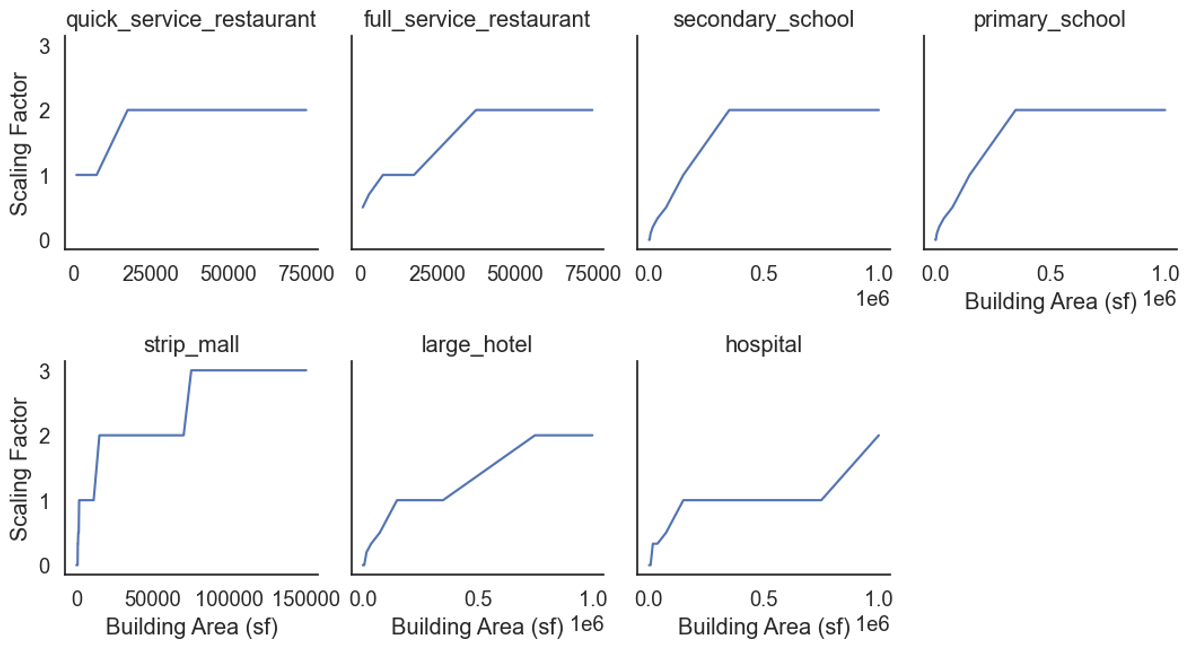
\includegraphics[
        page={1},
        %trim={1cm 18.3cm 1cm 1cm}, clip, % L B R T
        width=\textwidth]{figures/kitchen_equipment_count_scaling.png}
    \caption[Cooking equipment count scaling factors by building type and area]{Cooking equipment count scaling factors by building type and area.}
    \label{fig:cooking_equipment_count_scaling_factors_by_building_type_and_area}
\end{figure}

\section{Service Water Heating}

Service water heating (SWH) includes all water heating usage other than space heating and process requirements. This includes general water heating for uses such as sink faucets and showers, but also building-type-specific uses like commercial dish washing and laundry. This section describes how SWH equipment, fuel type, and usage is incorporated into ComStock models.   

\subsection{Service Water Heating Fuel Type}
\label{sec:SWH_Fuel_Type}

It would be logical to assume that the SWH system in a building would use the same fuel as the space heating system. An examination of the CBECS 2012 data \citep{eia2012cbecs} shows that this is the most common case, but it is not always true. In particular, it appears that building types that have large SWH loads, such as hotels and hospitals, are much more likely to use natural gas for SWH, regardless of what their space heating fuel is, presumably because of fuel cost differences. In contrast, building types with low SWH loads are more likely to use electricity for SWH, presumably because of the ease and cost of running wiring compared to installing natural gas piping.

To represent this variability, we used the CBECS 2012 data to create a distribution of SWH fuels for each combination of space heating fuel and building type. The resulting distribution of floor area served by various SWH fuels is shown in Figure \ref{fig:swh_fuel_dist}. As described in Section \ref{sec:HVAC_System_Type_Heating_Fuel_Type}, the prevalence of different space heating fuel varies considerably by county. Because the service water heating fuel depends on the space heating fuel, the probabilities at a stock level are heavily skewed toward the more common space heating fuels, as shown in Figure \ref{fig:swh_fuel_area}.

\begin{figure}[ht!]
  \centering
  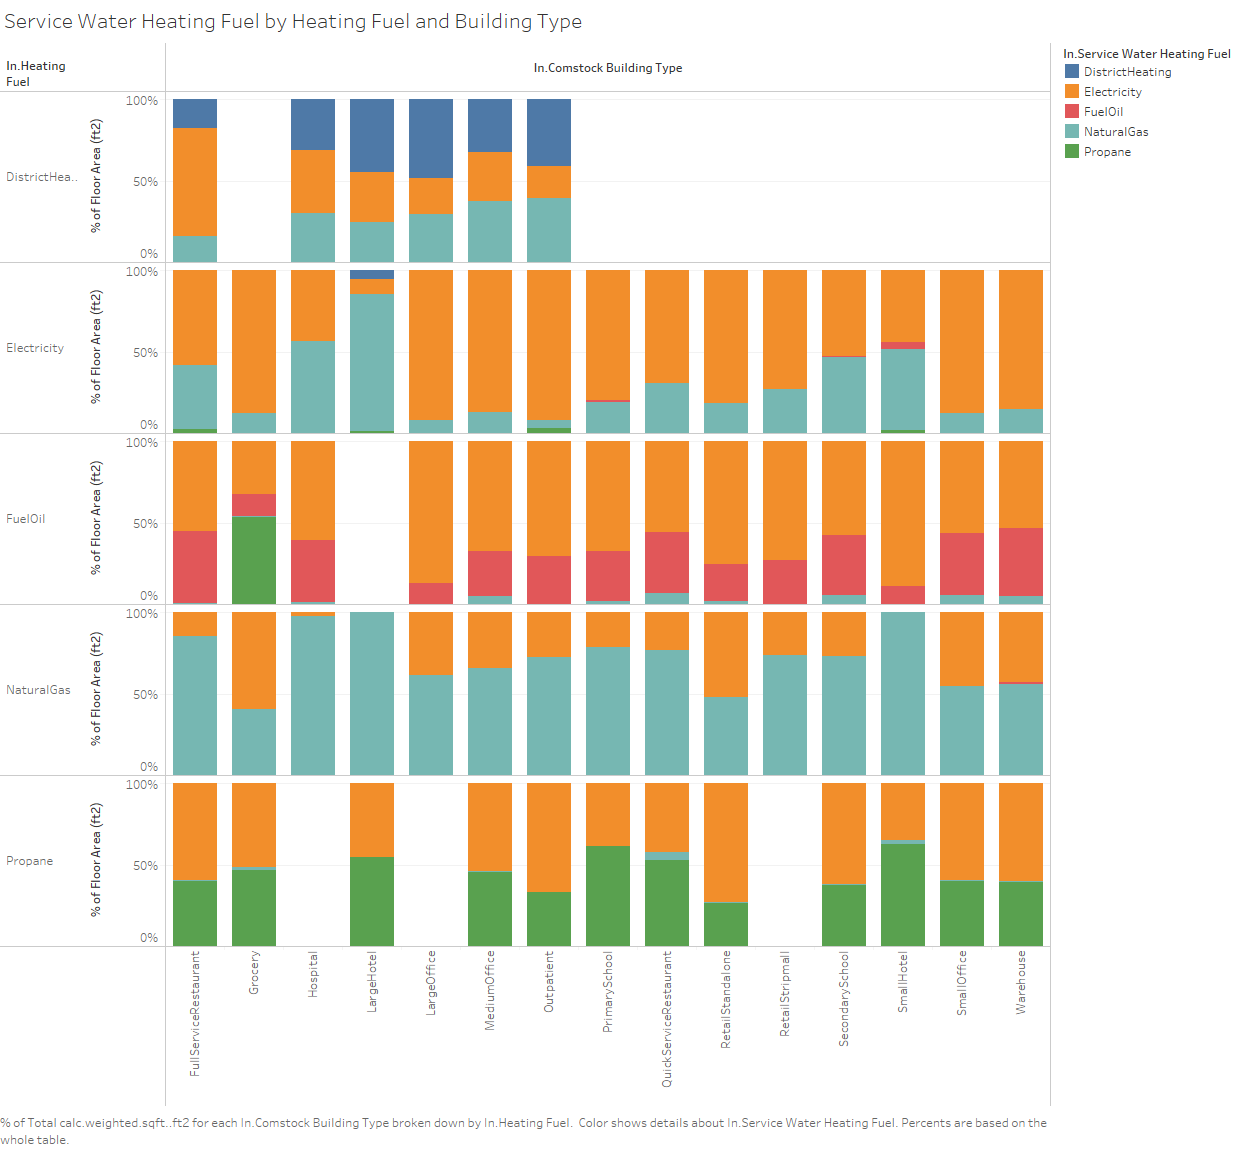
\includegraphics[width=\textwidth]{figures/swh_fuel_dist.png}
  \caption[Distribution of service water heating fuel by space heating fuel and building type]{Area-weighted distribution of service water heating fuel by space heating fuel and building type.}
  \label{fig:swh_fuel_dist}
\end{figure}

\begin{figure}[ht!]
  \centering
  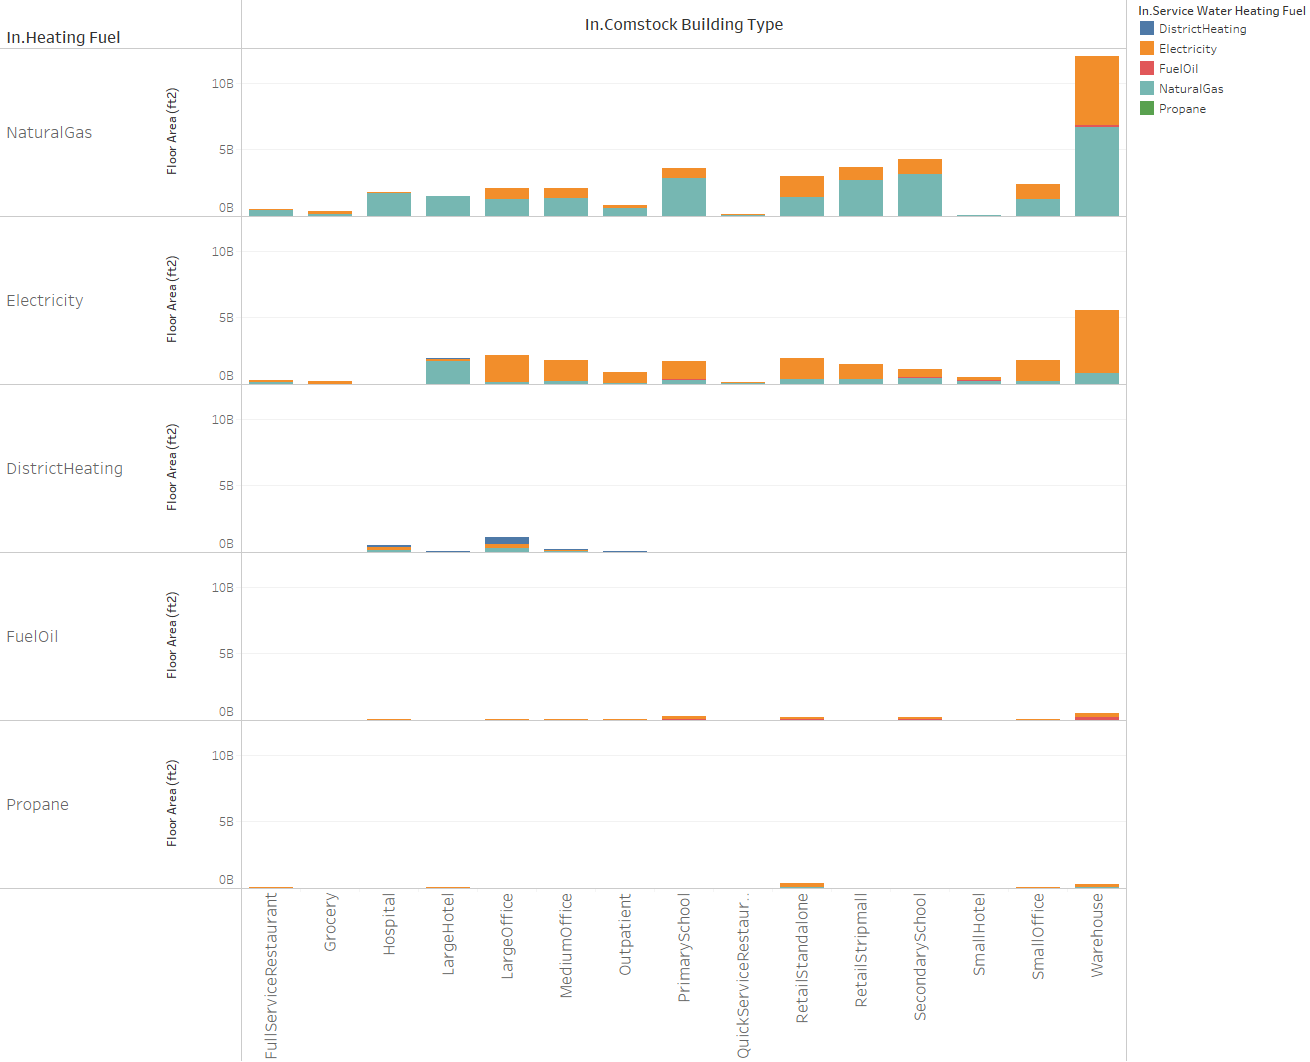
\includegraphics[width=\textwidth]{figures/swh_fuel_area.png}
  \caption[Floor area served by each service water heating fuel by space heating fuel and building type]{Floor area served by each service water heating fuel by space heating fuel and building type.}
  \label{fig:swh_fuel_area}
\end{figure}

\subsection{Service Water Heating System Type}

Service water heaters in ComStock models are all storage tank style, and are either fuel combustion (natural gas, fuel oil, or propane) or electric resistance, as discussed in  Section~\ref{sec:SWH_Fuel_Type}. Service water heaters with district heating as the fuel type receive hot water from off-site; therefore, these models do not include an on-site water heater. ComStock does not currently model instantaneous water heaters or heat pump water heaters. A single water heater is used to meet the demands of the entire building, unless a booster water loop is used, in which case a separate water heater system will be modeled for the boost loop. Booster loops are included for buildings with kitchen space types. These booster water heaters increase the temperature for some portion of the water for uses that need higher temperatures such as dishwashing. See Section~\ref{sec:space_type_ratios} for details on the space type ratios for each building type. In space types with booster water heaters, 60\% of peak flow is assigned to the booster water heater, and the remaining 40\% is assigned to the standard water heater.

The design temperature of standard water heaters in ComStock is 140°F with a 3.6°F deadband temperature difference allowance. Booster water heaters for kitchens have a target temperature of 180°F; this assumption comes from the DOE prototype models to account for dishwashing in kitchens. The ambient air temperature for tank heat loss is assumed to be 72°F. No parasitic losses or part load performance modifiers are included at this time.

%TODO: Discuss heat exchanger for booster water heaters? AP: I don't think this is necessary right now.

\subsection{Service Water Heating Efficiencies}

ComStock water heater efficiencies follow the requirements of ASHRAE-90.1. ComStock currently only models non-condensing units, so water heaters with a combustion fuel source are all roughly 80\% efficient, whereas electric resistance water heaters are roughly 100\% efficient. The efficiency parameters used to calculate the exact water heater efficiencies are summarized in Table~\ref{tab:water_heater_eff} based on SWH template, SWH fuel type, and SWH heater capacity. 

%\begin{table}
\centering
\scriptsize
\caption[Water Heater Efficiency]{Water Heating Efficiency by HVAC Template, Heater Capacity, and Fuel Type}
\label{tab:water_heater_eff}
\begin{tabular}{|p{0.5in}|p{0.5in}|p{0.3in}|p{0.3in}|p{0.3in}|p{0.3in}|p{0.3in}|p{0.3in}|p{0.3in}|p{0.3in}|p{0.3in}|p{0.3in}|p{1in}|}
\hline
\textbf{Template} &
  \textbf{Fuel Type} &
  \textbf{Minimum Capacity (Btu/hr)} &
  \textbf{Maximum Capacity (Btu/hr)} &
  \textbf{Energy Factor Base (\%)} &
  \textbf{Energy Factor Volume Derate (\%/gal)} &
  \textbf{Standby Loss Base (Btu/hr)} &
  \textbf{Standby Loss Capacity Allowance} &
  \textbf{Standby Loss Volume Allowance (Btu/hr*gal)} &
  \textbf{Hourly Loss Base (\%)} &
  \textbf{Hourly Loss Volume Allowance (\%/gal)} &
  \textbf{Thermal Efficiency (\%)} &
  \textbf{Notes} \\ \hline
\multirow{3}{*}{\parbox{0.5in}{\textbf{Pre-1980 Through 1980--2004}}} &
Electricity & 0 & 40945.99 & 0.93 & 0.00132 & & & & & & & \multirow{3}{*}{From DOE Reference Buildings} \\ \cline{2-12} &
Electricity & 40946 & No max & & & 20 & & 35 & & & & \\ \cline{2-12} &
Natural gas & 0 & No max & & & & & & & & 0.78 & \\ \hline
\multirow{4}{*}{\parbox{0.5in}{\textbf{90.1-2004 Through 2010}}} &
Electricity & 0 & 40945.99 & 0.93 & 0.00132 & & & & & & & \multirow{4}{*}{From 90.1 Table 7.8} \\ \cline{2-12} &
Electricity & 40946 & No max & & & 20 & & 35 & & & & \\ \cline{2-12} &
Natural gas & 0 & 74999.99 & 0.62 & 0.0019 & & & & & & & \\ \cline{2-12} &
Natural gas & 75000 & No max & & & & 800 & 110 & & & 0.8 & \\ \hline
\multirow{4}{*}{\textbf{90.1-2013}} &
Electricity & 0 & 40945.99 & 0.97 & 0.00132 & & & & & & & \multirow{4}{*}{From 90.1-2013 Table 7.8} \\ \cline{2-12} &
Electricity & 40946 & No max & & & & & & 0.3 & 27 & & \\ \cline{2-12} &
Natural gas & 0 & 74999.99 & 0.67 & 0.0019 & & & & & & & \\ \cline{2-12} &
Natural gas & 75000 & No max & & & & 800 & 110 & & & 0.8 & \\ \hline
\multirow{4}{*}{\parbox{0.5in}{\textbf{90.1-2016 Through 2019}}} &
Electricity & 0 & 40945.99 & 0.96 & 0.0003 & & & & & & & From 90.1 Table F-2, Rated Storage Volume \textless{}= 55 gal \\ \cline{2-13} &
Electricity & 40946 & No max & & & & & & 0.3 & 27 & & \\ \cline{2-13} &
Natural gas & 0 & 74999.99 & 0.675 & 0.0015 & & & & & & & From 90.1 Table F-2, Rated Storage Volume \textless{}= 55 gal \\ \cline{2-13} &
Natural gas & 75000 & No max & & & & 800 & 110 & & & 0.8 & \\ \hline
\end{tabular}
\end{table}

\subsection{Service Water Heating Usage and Schedules}

SWH usage for a given time step is based on a design peak gal/min flow rate multiplied by a usage fraction schedule. For example, if a given model has a design SWH flow rate of 10 gal/min, and the schedule value for the time step is 0.5, the SWH flow rate for the time step will be 5 gal/min. The flow rate values in ComStock come from the DOE prototype/reference building models, and are summarized in Tables~\ref{tab:swh_flow_rates_p1} through \ref{tab:swh_flow_rates_p3}.

In ComStock, the design flow rates are specified at the space type level. Then, these rates are aggregated to form a building-level design flow rate. The exception to this is SWH loads for kitchens, which are grouped into their own separate water heater system. These design flow rates are then multiplied by the usage fraction schedules, which specify the fraction of the design flow rate drawn for each time step. The usage fraction schedules in ComStock are derived from the DOE prototype/reference Buildings, and are summarized for each building type in Figures~\ref{fig:swh_sched_fsr} through ~\ref{fig:swh_sched_strip_mall}. The default schedule assignments for each space type and vintage are shown in Tables~\ref{tab:swh_flow_rates_p1} through ~\ref{tab:swh_flow_rates_p3}. However, these schedules are modified according to the hours of operation of the building, as described in Section~\ref{sec:hoo}. 

%TODO: Describe where flow rates and schedules come from
%TODO: Describe water heater tank and capacity sizing methods
%TODO: Describe the HX things for booster water heaters.

%\begin{table}
\centering
\small
\caption[Service Water Heating Flow Rate and Schedules Part 1]{Service Water Heating Flow Rate and Schedule Assignments Based on Template, Building Type, and Space Type (Part 1 of 3)}
\label{tab:swh_flow_rates_p1}
\begin{tabular}{|p{3cm}|p{3cm}|p{3cm}|p{3cm}|p{3cm}|}
\hline
\textbf{Template} &
  \textbf{Building Type} &
  \textbf{Space Type} &
  \textbf{Service Water   Heating Peak Flow per Area (gal/h*ft$^2$)} &
  \textbf{Service Water   Heating Schedule} \\ \hline
\textbf{All}                     & FullServiceRestaurant & Kitchen     & 0.08861 & RestaurantSitDown   BLDG\_SWH\_SCH           \\ \hline
\textbf{All}                     & Hospital              & ER\_Exam    & 0.00333 & Hospital   BLDG\_SWH\_EXTD\_SCH              \\ \hline
\textbf{All}                     & Hospital              & ER\_Trauma  & 0.00333 & Hospital   BLDG\_SWH\_EXTD\_SCH              \\ \hline
\textbf{All}                     & Hospital              & ER\_Triage  & 0.00333 & Hospital   BLDG\_SWH\_EXTD\_SCH              \\ \hline
\textbf{All}                     & Hospital              & Kitchen     & 0.015   & Hospital   BLDG\_SWH\_EXTD\_SCH              \\ \hline
\textbf{All}                     & Hospital              & Lab         & 0.0007  & Hospital BLDG\_SWH\_SCH                      \\ \hline
\textbf{All}                     & Hospital              & OR          & 0.00333 & Hospital BLDG\_SWH\_SCH                      \\ \hline
\textbf{All}                     & Hospital              & PatRoom     & 0.00357 & Hospital   BLDG\_SWH\_EXTD\_SCH              \\ \hline
\textbf{All}                     & Hospital              & PhysTherapy & 0.00019 & Hospital BLDG\_SWH\_SCH                      \\ \hline
\textbf{All}                     & Hospital              & Radiology   & 0.00019 & Hospital   BLDG\_SWH\_EXTD\_SCH              \\ \hline
\textbf{All}                     & LargeHotel            & GuestRoom   & 0.00298 & HotelLarge   GuestRoom\_SWH\_Sch             \\ \hline
\textbf{All}                     & LargeHotel            & GuestRoom2  & 0.00473 & HotelLarge   GuestRoom\_SWH\_Sch             \\ \hline
\textbf{All}                     & LargeHotel            & GuestRoom2  & 0.08994 & HotelLarge   GuestRoom\_SWH\_Sch             \\ \hline
\textbf{All}                     & LargeHotel            & GuestRoom3  & 0.00298 & HotelLarge   GuestRoom\_SWH\_Sch             \\ \hline
\textbf{All}                     & LargeHotel            & GuestRoom4  & 0.00473 & HotelLarge   GuestRoom\_SWH\_Sch             \\ \hline
\textbf{All}                     & LargeHotel            & GuestRoom4  & 0.0426  & HotelLarge   GuestRoom\_SWH\_Sch             \\ \hline
\textbf{All}                     & LargeHotel            & GuestRoom5  & 0.0036  & HotelLarge   GuestRoom\_SWH\_Sch             \\ \hline
\textbf{All}                     & LargeHotel            & GuestRoom6  & 0.00294 & HotelLarge   GuestRoom\_SWH\_Sch             \\ \hline
\textbf{All}                     & LargeHotel            & GuestRoom7  & 0.00215 & HotelLarge   GuestRoom\_SWH\_Sch             \\ \hline
\textbf{All}                     & LargeHotel            & GuestRoom8  & 0.00473 & HotelLarge   GuestRoom\_SWH\_Sch             \\ \hline
\textbf{All}                     & LargeHotel            & Kitchen     & 0.1196  & HotelLarge   BLDG\_SWH\_SCH                  \\ \hline
\textbf{90.1-2004 and Later} & LargeHotel            & Laundry     & 0.18643 & HotelLarge   LaundryRoom\_SWH\_Sch\_Post2004 \\ \hline
\textbf{Pre 90.1-2004}  & LargeHotel            & Laundry     & 0.18643 & HotelLarge   LaundryRoom\_SWH\_Sch\_Pre2004  \\ \hline
\end{tabular}
\end{table}
%\begin{table}
\centering
\small
\caption[Service Water Heating Flow Rate and Schedules Part 2]{Service Water Heating Flow Rate and Schedule Assignments Based on Template, Building Type, and Space Type (Part 2 of 3)}
\label{tab:swh_flow_rates_p2}
\begin{tabular}{|p{3cm}|p{3cm}|p{3cm}|p{3cm}|p{3cm}|}
\hline
\textbf{Template} &
  \textbf{Building Type} &
  \textbf{Space Type} &
  \textbf{Service Water   Heating Peak Flow per Area (gal/h*ft$^2$)} &
  \textbf{Service Water   Heating Schedule} \\ \hline
\textbf{Pre 90.1-2004}  & Office          & MediumOffice -   Elec/MechRoom       & 0.01845 & Medium Office Bldg   Swh           \\ \hline
\textbf{90.1-2004 and Later} & Office          & MediumOffice -   Elec/MechRoom       & 0.03171 & OfficeMedium   BLDG\_SWH\_SCH      \\ \hline
\textbf{All}                     & Office          & Restroom                             & 0.20471 & OfficeLarge   BLDG\_SWH\_SCH       \\ \hline
\textbf{All}                     & Office          & SmallOffice -   Elec/MechRoom        & 0.00055 & OfficeSmall   BLDG\_SWH\_SCH       \\ \hline
\textbf{Pre 90.1-2004}  & Office          & WholeBuilding - Lg   Office          & 0.00013 & OfficeLarge   BLDG\_SWH\_SCH       \\ \hline
\textbf{90.1-2004 and Later} & Office          & WholeBuilding - Lg   Office          & 0.00052 & OfficeLarge   BLDG\_SWH\_SCH       \\ \hline
\textbf{All}                     & Office          & WholeBuilding - Lg   Office-basement & 0.00052 & OfficeLarge   BLDG\_SWH\_SCH       \\ \hline
\textbf{All}                     & Office          & WholeBuilding - Lg   Office-others   & 0.00052 & OfficeLarge   BLDG\_SWH\_SCH       \\ \hline
\textbf{Pre 90.1-2004}  & Office          & WholeBuilding - Md   Office          & 0.00055 & OfficeMedium   BLDG\_SWH\_SCH      \\ \hline
\textbf{90.1-2004 and Later} & Office          & WholeBuilding - Md   Office          & 0.00095 & OfficeMedium   BLDG\_SWH\_SCH      \\ \hline
\textbf{All}                     & Office          & WholeBuilding - Sm   Office          & 0.00055 & OfficeSmall   BLDG\_SWH\_SCH       \\ \hline
\textbf{All}                     & Retail          & Back\_Space                          & 0.00535 & RetailStandalone   BLDG\_SWH\_SCH  \\ \hline
\textbf{All}                     & SecondarySchool & Gym                                  & 0.0075  & SchoolSecondary   BLDG\_SWH\_SCH   \\ \hline
\textbf{All}                     & SecondarySchool & Gym - audience                       & 0.0075  & SchoolSecondary   BLDG\_SWH\_SCH   \\ \hline
\textbf{All}                     & SecondarySchool & Kitchen                              & 0.0572  & SchoolSecondary   BLDG\_SWH\_SCH   \\ \hline
\textbf{All}                     & SecondarySchool & Restroom                             & 0.0231  & SchoolSecondary   BLDG\_SWH\_SCH   \\ \hline
\textbf{All}                     & SmallHotel      & GuestRoom                            & 0.00499 & HotelSmall   GuestRoom\_SHW\_Sch   \\ \hline
\textbf{Pre 90.1-2004}  & SmallHotel      & GuestRoom123Occ                      & 0.00499 & HotelSmall   GuestRoom\_SHW\_Sch   \\ \hline
\textbf{90.1-2004 and Later} & SmallHotel      & GuestRoom123Occ                      & 0.00632 & HotelSmall   GuestRoom\_SHW\_Sch   \\ \hline
\textbf{Pre 90.1-2004}  & SmallHotel      & GuestRoom123Vac                      & 0.00499 & HotelSmall   GuestRoom\_SHW\_Sch   \\ \hline
\textbf{90.1-2004 and Later} & SmallHotel      & GuestRoom123Vac                      & 0.00632 & HotelSmall AlwaysOff               \\ \hline
\textbf{Pre 90.1-2004}  & SmallHotel      & GuestRoom4Occ                        & 0.00499 & HotelSmall   GuestRoom\_SHW\_Sch   \\ \hline
\textbf{90.1-2004 and Later} & SmallHotel      & GuestRoom4Occ                        & 0.00632 & HotelSmall   GuestRoom\_SHW\_Sch   \\ \hline
\textbf{Pre 90.1-2004}  & SmallHotel      & GuestRoom4Vac                        & 0.00499 & HotelSmall   GuestRoom\_SHW\_Sch   \\ \hline
\textbf{90.1-2004 and Later} & SmallHotel      & GuestRoom4Vac                        & 0.00632 & HotelSmall AlwaysOff               \\ \hline
\textbf{All}                     & SmallHotel      & Laundry                              & 0.0641  & HotelSmall   LaundryRoom\_SHW\_Sch \\ \hline
\end{tabular}
\end{table}
%\begin{table}
\centering
\small
\caption[Service Water Heating Flow Rate and Schedules Part 3]{Service Water Heating Flow Rate and Schedule Assignments Based on Template, Building Type, and Space Type (part 3 of 3)}
\label{tab:swh_flow_rates_p3}
\begin{tabular}{|p{3cm}|p{3cm}|p{3cm}|p{3cm}|p{3cm}|}
\hline
\textbf{Template} &
  \textbf{Building Type} &
  \textbf{Space Type} &
  \textbf{Service Water   Heating Peak Flow per Area (gal/h*ft$^2$)} &
  \textbf{Service Water   Heating Schedule} \\ \hline
\textbf{Pre 90.1-2004}  & Outpatient             & Anesthesia      & 0.00926 & OutPatientHealthCare   BLDG\_SWH\_SCH\_Pre2004 \\ \hline
\textbf{90.1-2004 and Later} & Outpatient             & Anesthesia      & 0.01852 & OutPatientHealthCare   BLDG\_SWH\_SCH          \\ \hline
\textbf{Pre 90.1-2004}  & Outpatient             & MRI             & 0.00227 & OutPatientHealthCare   BLDG\_SWH\_SCH\_Pre2004 \\ \hline
\textbf{90.1-2004 and Later} & Outpatient             & MRI             & 0.00455 & OutPatientHealthCare   BLDG\_SWH\_SCH          \\ \hline
\textbf{Pre 90.1-2004}  & Outpatient             & MRI\_Control    & 0.00595 & OutPatientHealthCare   BLDG\_SWH\_SCH\_Pre2004 \\ \hline
\textbf{90.1-2004 and Later} & Outpatient             & MRI\_Control    & 0.0119  & OutPatientHealthCare   BLDG\_SWH\_SCH          \\ \hline
\textbf{Pre 90.1-2004}  & Outpatient             & OR              & 0.01271 & OutPatientHealthCare   BLDG\_SWH\_SCH\_Pre2004 \\ \hline
\textbf{90.1-2004 and Later} & Outpatient             & OR              & 0.02542 & OutPatientHealthCare   BLDG\_SWH\_SCH          \\ \hline
\textbf{Pre 90.1-2004}  & Outpatient             & PACU            & 0.00316 & OutPatientHealthCare   BLDG\_SWH\_SCH\_Pre2004 \\ \hline
\textbf{90.1-2004 and Later} & Outpatient             & PACU            & 0.00633 & OutPatientHealthCare   BLDG\_SWH\_SCH          \\ \hline
\textbf{Pre 90.1-2004}  & Outpatient             & PhysicalTherapy & 0.00106 & OutPatientHealthCare   BLDG\_SWH\_SCH\_Pre2004 \\ \hline
\textbf{90.1-2004 and Later} & Outpatient             & PhysicalTherapy & 0.00211 & OutPatientHealthCare   BLDG\_SWH\_SCH          \\ \hline
\textbf{Pre 90.1-2004}  & Outpatient             & PreOp           & 0.0038  & OutPatientHealthCare   BLDG\_SWH\_SCH\_Pre2004 \\ \hline
\textbf{90.1-2004 and Later} & Outpatient             & PreOp           & 0.00759 & OutPatientHealthCare   BLDG\_SWH\_SCH          \\ \hline
\textbf{Pre 90.1-2004}  & Outpatient             & ProcedureRoom   & 0.00351 & OutPatientHealthCare   BLDG\_SWH\_SCH\_Pre2004 \\ \hline
\textbf{90.1-2004 and Later} & Outpatient             & ProcedureRoom   & 0.00702 & OutPatientHealthCare   BLDG\_SWH\_SCH          \\ \hline
\textbf{Pre 90.1-2004}  & Outpatient             & Xray            & 0.00111 & OutPatientHealthCare   BLDG\_SWH\_SCH\_Pre2004 \\ \hline
\textbf{90.1-2004 and Later} & Outpatient             & Xray            & 0.00222 & OutPatientHealthCare   BLDG\_SWH\_SCH          \\ \hline
\textbf{All}                     & PrimarySchool          & Kitchen         & 0.05531 & SchoolPrimary   BLDG\_SWH\_SCH                 \\ \hline
\textbf{All}                     & PrimarySchool          & Restroom        & 0.02763 & SchoolPrimary   BLDG\_SWH\_SCH                 \\ \hline
\textbf{Pre 90.1-2004}  & QuickServiceRestaurant & Kitchen         & 0.032   & QuickServiceRestaurant   Bldg Swh              \\ \hline
\textbf{90.1-2004 and Later} & QuickServiceRestaurant & Kitchen         & 0.032   & RestaurantFastFood   BLDG\_SWH\_SCH            \\ \hline
\end{tabular}
\end{table}






\section{Heating, Ventilating, Air Conditioning, and Refrigeration}
\label{sec:HVAC_System_Type_Heating_Fuel_Type}

\subsection{HVAC System Heating Fuel Type}

Commercial HVAC equipment can use various heating fuel types, with the most common being natural gas, electricity, propane, fuel oil, and district heating. To reflect the variability of heating fuels in the real building stock, the ComStock workflow creates probability distributions of heating fuel types per building type at the county level. These distributions are used to assign a heating fuel type to each ComStock building model during the sampling process.

The probability distributions are informed by two data sources. First, there are the CBECS 2012 microdata, which include data on heating fuel(s), building type, and census division for the surveyed buildings. This data can be used to produce probability distributions for heating fuel by building type at the census division level. However, several data sources suggest notable variation within census divisions, which indicates that increased granularity may be needed (beyond what CBECS can provide). The heating fuel type probability distributions used in ResStock---which provides data for residential buildings at the county level---were used to add granularity. However, initial comparisons showed discrepancies between the ResStock data and the CBECS data, which is likely due to inherent differences between residential and commercial buildings. This indicated that the ResStock data should not be used directly. To rectify this, the county-level ResStock data were scaled to align with the CBECS data. This preserved the county-level variation in fuel type prevalence provided by the ResStock data, while also preserving the census division totals provided by the CBECS commercial data. District heating values were not available in the ResStock data, so the per-building-type CBECS values were used for all counties in a given census division.

In some cases, filtering down to a specific region and building type in the CBECS data yields very few samples. This can lead to unreliable conclusions for a region. To mitigate this, we took a blended approach, where some fraction of the CBECS region fuel type percentage comes from the regional samples only, and some fraction comes from the national sample for the building type. If more than 15 samples exist for a given building type and region, then 100\% of the fuel type prevalence comes from that specific region. (The threshold of 15 samples was selected baced on engineering judgment to balance process reliability and regional variability.) If there are fewer than 15 samples, the number of samples divided by 15 will be the fraction used for the region, and the remainder will use the national numbers. For example, if a region has only 12 office samples, 80\% (12\//15) of the effective CBECS regional value will come from the CBECS region, and the other 20\% will come from the national CBECS value for the building type. This will cause region/building type combinations with lower sample sizes to have a stronger inheritance of the national characteristics than the regional characteristics when we lack sufficient evidence to support this level of detail.

Some commercial building HVAC systems use multiple fuel types. For example, a VAV system with a gas furnace in the air handling unit and electric resistance coils in the reheat boxes, or a gas furnace DOAS with variable refrigerant flow (VRF) heat pumps serving the zones. This can complicate the categorization of these systems into a single primary fuel type. To address this, we determine the primary heating fuel type for the mixed fuel systems. The primary heating fuel is the heating fuel expected to carry the majority of the heating load. For example, the previously mentioned example of a VAV system with gas heat at the air handler and electric reheat would be classified as an electric-heated system, since the majority of heating for multizone VAV systems usually comes from the reheat. A full list of ComStock HVAC systems and their fuel type categories are shown in Table~\ref{tab:hvac_system_heating_fuel_categories}. Further detail on model HVAC system assignment methodology can be found in Section~\ref{sec:HVAC_System_Type}.

Figure~\ref{fig:fuel_cbecs_v_cstock} compares the prevalence of heating fuel type by stock floor area for CBECS 2012 and ComStock, by building type. In most cases, ComStock closely aligns to the CBECS 2012 values. However, there are some differences between the two sources due to randomness in the sampling process and from the use of other data sources to achieve county-level granularity in fuel type prevalence. The largest difference is in small hotels where ComStock shows 87\% of the floor area using electric heating while CBECS suggest 74\%, an absolute difference of 12\%.

\begin{figure}
  \centering
  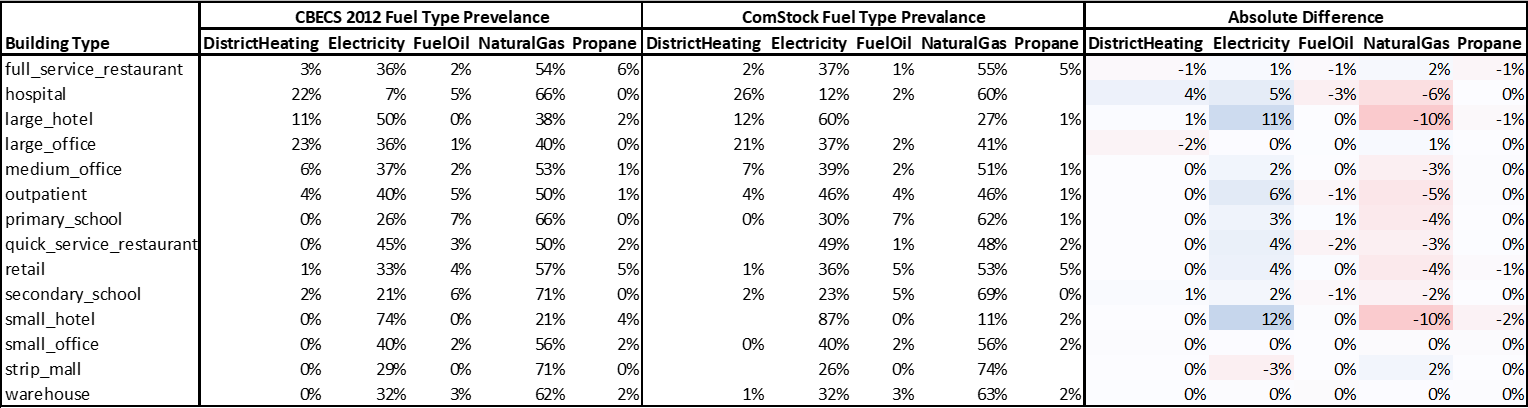
\includegraphics[width=1.10\textwidth]{figures/cbecs_comstock_fuel_type_comparison.png}
  \caption[Comparison of heating fuel type prevalence by floor area between CBECS 2012 and ComStock.]{Comparison of heating fuel type prevalence by floor area between CBECS 2012 and ComStock.}
  \label{fig:fuel_cbecs_v_cstock}
\end{figure}

The county-level prevalences of different heating fuel types are shown in Figure~\ref{fig:map_naturalgas} (natural gas), Figure~\ref{fig:map_electricity} (electricity), Figure~\ref{fig:map_fueloil} (fuel oil), Figure~\ref{fig:map_propane} (propane), and Figure~\ref{fig:map_district} (district heating).

\begin{figure}
  \centering
  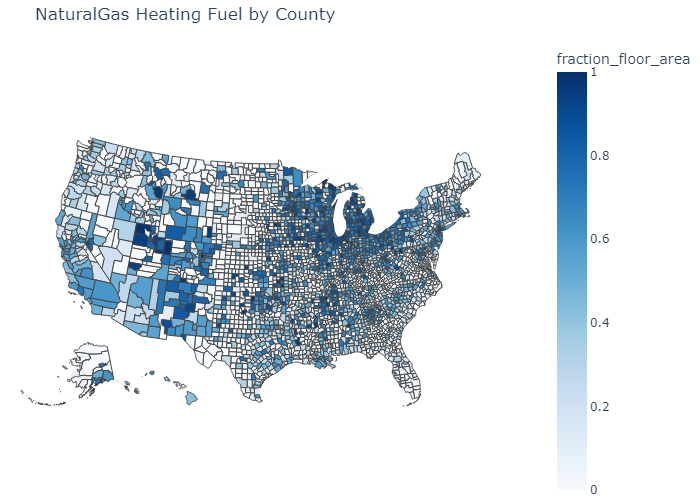
\includegraphics[width=0.8\textwidth]{figures/map_naturalgas.png}
  \caption[Fraction of ComStock models using natural gas heating/water heating per county]{Fraction of ComStock models using natural gas heating per county.}
  \label{fig:map_naturalgas}
\end{figure}

\begin{figure}
  \centering
  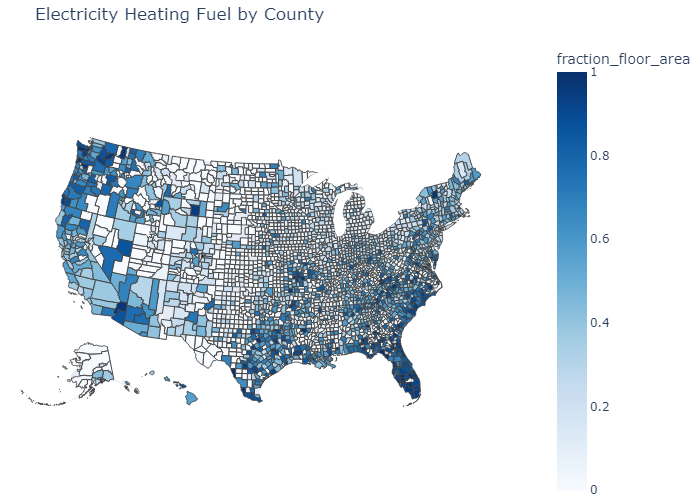
\includegraphics[width=0.8\textwidth]{figures/map_electricity.png}
  \caption[Fraction of ComStock models using electric heating/water heating per county]{Fraction of ComStock models using electric heating per county.}
  \label{fig:map_electricity}
\end{figure}

\begin{figure}
  \centering
  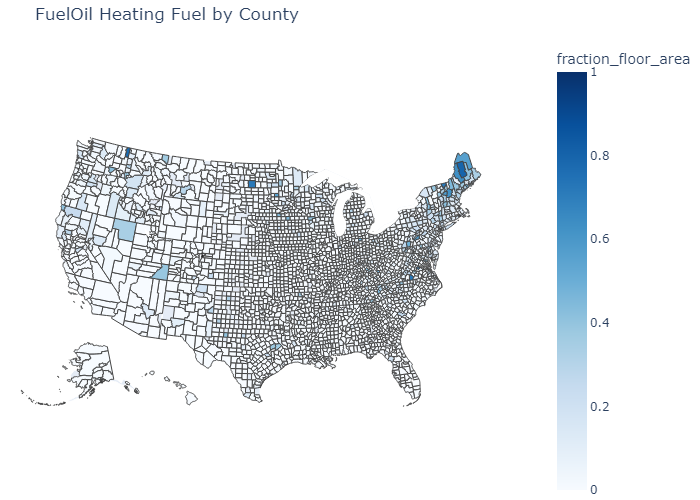
\includegraphics[width=0.8\textwidth]{figures/map_fueloil.png}
  \caption[Fraction of ComStock models using fuel oil heating/water heating per county]{Fraction of ComStock models using fuel oil heating per county.}
  \label{fig:map_fueloil}
\end{figure}

\begin{figure}
  \centering
  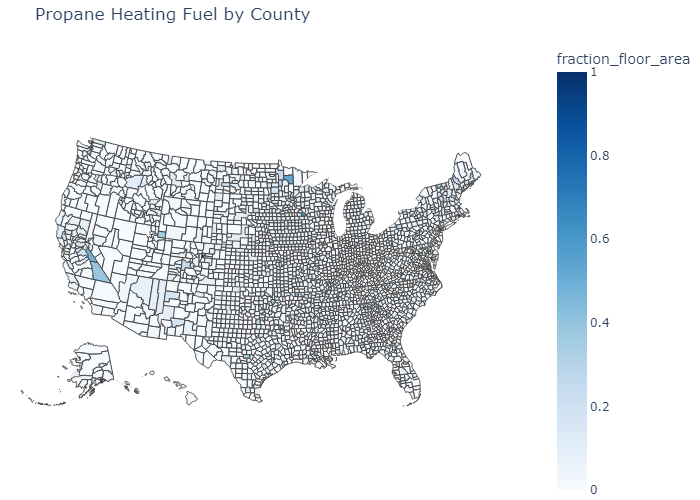
\includegraphics[width=0.8\textwidth]{figures/map_propane.png}
  \caption[Fraction of ComStock models using propane heating/water heating per county]{Fraction of ComStock models using propane heating per county.}
  \label{fig:map_propane}
\end{figure}

\begin{figure}
  \centering
  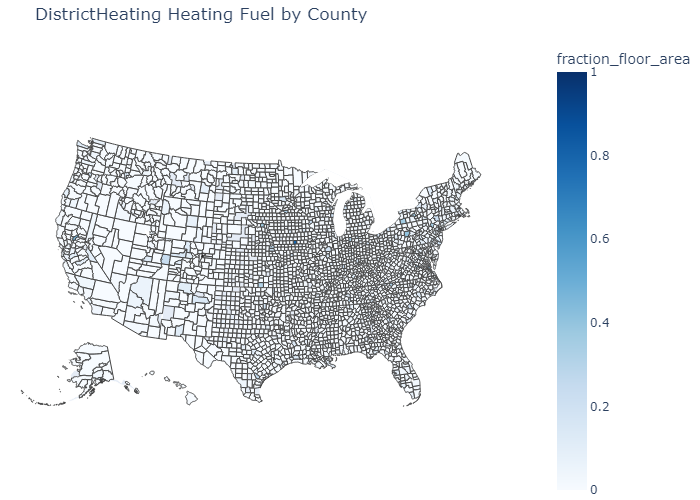
\includegraphics[width=0.8\textwidth]{figures/map_districtheating.png}
  \caption[Fraction of ComStock models using district heating/water heating per county]{Fraction of ComStock models using district heating per county.}
  \label{fig:map_district}
\end{figure}



%figures moved to appendix

\vspace{5mm}
\subsection{HVAC System Types Probability Distributions}
\label{sec:HVAC_System_Type}

Each ComStock model is assigned a comprehensive HVAC system type. The full list of ComStock HVAC system types is shown in Table~\ref{tab:hvac_system_heating_fuel_categories}. HVAC system types are assigned to ComStock models through sampling informed by representative probability distributions. These probability distributions depend on building type, census division, and heating fuel type. For example, the distributions provide the fraction of gas-heated retail buildings in the West North Central Census Division that use each HVAC system type from Table~\ref{tab:hvac_system_heating_fuel_categories}. The probability distributions are derived from CBECS 2012 microdata, which include data on building type, census division, heating fuel type, and HVAC system type.

\begin{table}[hb!]
\small
\centering
\caption[Fuel Type Category for ComStock HVAC System Types]{Fuel Type Category for ComStock HVAC System Types}
\label{tab:hvac_system_heating_fuel_categories}
\begin{tabular}{|l|l|}
\hline
\textbf{HVAC System Type}                                   & \textbf{Heating Fuel Category} \\ \hline
Packaged variable air volume (PVAV) with gas heat with electric reheat                     & Electricity                           \\ \hline
DOAS with fan coil district chilled water with district hot water & District\_Heating        \\ \hline
Variable air volume (VAV) district chilled water with district hot water reheat         & District\_Heating        \\ \hline
PSZ-AC with gas coil                                        & Fuel                           \\ \hline
VAV chiller with PFP boxes                                  & Electricity                    \\ \hline
VAV chiller with gas boiler reheat                          & Fuel                           \\ \hline
VAV air-cooled chiller with gas boiler reheat               & Fuel                           \\ \hline
Packaged terminal air conditioner (PTAC) with electric coil                                     & Electricity                    \\ \hline
PSZ-AC with gas boiler                                      & Fuel                           \\ \hline
VAV air-cooled chiller with district hot water reheat       & District\_Heating              \\ \hline
Residential AC with residential forced air furnace          & Fuel                           \\ \hline
PSZ-AC with electric coil                                   & Electricity                    \\ \hline
VAV air-cooled chiller with parallel fan-powered (PFP) boxes                       & Electricity                    \\ \hline
Packaged terminal heat pump (PTHP)                                                        & Electricity                    \\ \hline
PVAV with gas boiler reheat                                 & Fuel                           \\ \hline
PVAV with PFP boxes                                         & Electricity                    \\ \hline
VAV chiller with district hot water reheat                  & District\_Heating              \\ \hline
DOAS with fan coil air-cooled chiller with boiler           & Fuel                           \\ \hline
DOAS with fan coil chiller with boiler                      & Fuel                           \\ \hline
DOAS with variable refrigerant flow (VRF)                                               & Electricity                    \\ \hline
Residential forced air furnace                              & Fuel                           \\ \hline
DOAS with water source heat pumps with ground source heat pump    & Electricity              \\ \hline
DOAS with water source heat pumps cooling tower with boiler & Electricity                    \\ \hline
Direct evap coolers with forced air furnace                 & Fuel                           \\ \hline
VAV district chilled water with PFP boxes                   & Electricity                    \\ \hline
PVAV with district hot water reheat                         & District\_Heating              \\ \hline
DOAS with fan coil chiller with district hot water          & District\_Heating              \\ \hline
Direct evap coolers with baseboard gas boiler               & Fuel                           \\ \hline
PTAC with gas boiler                                        & Fuel                           \\ \hline
Packaged single-zone air conditioner (PSZ-AC) with district hot water                              & District\_Heating              \\ \hline
Packaged single-zone heat pump (PSZ-HP)                                                      & Electricity                    \\ \hline
Gas unit heaters                                            & Fuel                           \\ \hline
DOAS with fan coil chiller with baseboard electric          & Electricity                    \\ \hline
PSZ-AC district chilled water with district hot water       & District\_Heating              \\ \hline
Direct evap coolers with baseboard electric                 & Electricity                    \\ \hline
VAV district chilled water with gas boiler reheat           & Fuel                           \\ \hline
Baseboard electric                                          & Electricity                    \\ \hline
DOAS with fan coil air-cooled chiller with district hot water     & District\_Heating        \\ \hline
PSZ-AC district chilled water with electric coil            & Electricity                    \\ \hline
DOAS with fan coil district chilled water with boiler       & Fuel                           \\ \hline
PTAC with gas coil                                          & Fuel                           \\ \hline
DOAS with fan coil district chilled water with baseboard electric & Electricity              \\ \hline
Baseboard gas boiler                                        & Fuel                           \\ \hline
PTAC with baseboard district hot water                      & District\_Heating              \\ \hline
DOAS with fan coil air-cooled chiller with baseboard electric     & Electricity       \\ \hline
\end{tabular}
\end{table}

\subsubsection{CBECS HVAC System Type Analysis}

To derive probability distributions of HVAC system types from the CBECS data, we first assigned one of the comprehensive ComStock HVAC system types shown in Table~\ref{tab:hvac_system_heating_fuel_categories} to the CBECS microdata samples. Historically, this analysis was based solely on the CBECS 2012 data set; however, our updated methodology now integrates data from both the CBECS 2012 and CBECS 2018 data sets. To combine these data sources, we apply a weighted average based on the number of samples from each data set to ensure appropriate representation.

CBECS includes questions regarding the primary HVAC system type of the building; however, it also contains dozens of additional questions about HVAC system components, fuel types, and technologies. In several cases, these responses may conflict with one another, making it difficult to derive a deterministic HVAC system type for the CBECS building samples. Interpretation of the numerous HVAC characteristics into a complete HVAC system type needed for energy modeling involves user discretion and judgment. On multiple occasions, the combinations of survey responses related to the HVAC system were questionable, incomplete, or conflicting based on engineering judgment. This could be due to the survey respondent lacking information about the nuances of the building's HVAC system, the survey respondent skipping relevant questions, or the building having multiple system types, perhaps due to various activities in the building or retrofits and expansions over time. Any of these issues could create a combination of equipment for a CBECS sample that would be difficult to translate into a single, comprehensive HVAC system type without firsthand knowledge of the building. Thus, reliably discerning an HVAC system type from the survey questions can be challenging for some of the CBECS samples and requires some degree of assumption.

Based on survey responses, some CBECS samples appear to utilize multiple types of HVAC systems. For example, one sample responded affirmatively to having a chiller, packaged terminal air conditioners (PTACs), heat pumps, and a swamp cooler. However, there is no indication as to the fraction of the building serving each system type in the survey. Additionally, ComStock is not trying to model buildings with several HVAC system types. To address this, we needed to determine prioritization rules when multiple system types for a single CBECS sample appeared to be prevalent. To achieve this, we grouped systems into the following four categories: VAVs, single-zone RTU, DOAS with zone terminal units (e.g., DOAS with heat pumps, VRF), and miscellaneous single-zone equipment.

There were several cases where the assigned HVAC system for a CBECS sample was unlikely given the size and type of the building. For example, only a small percentage of small office buildings would be expected to use large, multi-zone VAV systems. Similarly, only a small percentage of very large office buildings would be expected to use single-zone RTUs or zone terminal equipment with no DOAS. To address this, we introduced "size bins" to our distributions to ensure system types were correctly assigned based on building size. These size bins were incorporated into the sampling methodology, described in Section \ref{chap:3_sampling}, to further refine system type assignments and improve the alignment between system types and building characteristics. Additional heating-only system types were assigned to building zones whose thermostat setpoints (see \ref{section:therm_setpoints}) described heating-only operation. This primarily affected warehouse buildings in California, representing approximately 13\% of the total stock warehouse floor area, which moved from the primary system type to heating-only gas unit heaters or electric baseboard systems, depending on primary heating fuel source.

Overall, we produced 1,162 probability distributions from the combined CBECS 2012 and 2018 HVAC analysis, with dependencies based on building type, size bin, heating fuel, and census region. These distributions are used with the ComStock sampling process, described in Section \ref{chap:3_sampling}, which ensures that HVAC system types are applied to the correct proportion of models. The prevalence of each HVAC system type in ComStock for all building types is shown in Figure~\ref{fig:hvac_sys_type_prevalence} through Figure~\ref{fig:hvac_sys_type_prevalence_warehouse}.

% AP Decided not to show this table as the information is conveyed more usefully in the figures below
% \begin{center}
\begin{longtable}{|p{5cm}|p{1.5cm}|p{1.5cm}|p{1.5cm}|p{1.5cm}|p{1.5cm}|p{1.5cm}|p{1.5cm}|p{1.5cm}|p{1.5cm}|p{1.5cm}|p{1.5cm}|p{1.5cm}|p{1.5cm}|p{1.5cm}|}
\caption[HVAC System Type Prevalence]{HVAC System Type Prevalence by Building Type} \\ \hline
\label{tab:hvac_system_types}
\textbf{ComStock System Type} &
  \textbf{full service restaurant} &
  \textbf{hospital} &
  \textbf{large hotel} &
  \textbf{large office} &
  \textbf{medium office} &
  \textbf{outpatient} &
  \textbf{primary school} &
  \textbf{quick service restaurant} &
  \textbf{retail} &
  \textbf{secondary school} &
  \textbf{small hotel} &
  \textbf{small office} &
  \textbf{strip mall} &
  \textbf{warehouse} \\ \hline
\endfirsthead
\multicolumn{2}{c} {{\bfseries \tablename \thetable{} -- continued from previous page}} \\ \hline
\textbf{ComStock System Type} &
  \textbf{full service restaurant} &
  \textbf{hospital} &
  \textbf{large hotel} &
  \textbf{large office} &
  \textbf{medium office} &
  \textbf{outpatient} &
  \textbf{primary school} &
  \textbf{quick service restaurant} &
  \textbf{retail} &
  \textbf{secondary school} &
  \textbf{small hotel} &
  \textbf{small office} &
  \textbf{strip mall} &
  \textbf{warehouse} \\ \hline
\endhead
\small
Baseboard electric                                                & 0    & 0    & 0    & 0    & 0    & 0    & 0    & 0    & 0.5  & 0    & 0    & 0    & 0    & 0.6  \\ \hline
Baseboard gas boiler                                              & 0    & 0    & 0    & 0    & 0    & 0    & 0    & 0    & 0    & 0    & 0    & 0    & 0    & 0    \\ \hline
DOAS with VRF                                                     & 0    & 0    & 0.4  & 0.8  & 1.7  & 1.3  & 0.3  & 0    & 0    & 0    & 0    & 1.5  & 0    & 0.3  \\ \hline
DOAS with fan coil air-cooled chiller with baseboard electric     & 0    & 0    & 0.1  & 0    & 0    & 0    & 0    & 0    & 0    & 0    & 0    & 0    & 0    & 0    \\ \hline
DOAS with fan coil air-cooled chiller with boiler                 & 0    & 0.2  & 2.7  & 0.3  & 0    & 0.5  & 0.9  & 0    & 0    & 1.9  & 0    & 0    & 0    & 0    \\ \hline
DOAS with fan coil air-cooled chiller with district hot water     & 0    & 0.1  & 0    & 1.1  & 0    & 0    & 0    & 0    & 0    & 0    & 0    & 0    & 0    & 0    \\ \hline
DOAS with fan coil chiller with baseboard electric                & 0    & 0    & 0.6  & 0.1  & 0    & 0    & 0    & 0    & 0    & 0    & 0    & 0    & 0    & 0    \\ \hline
DOAS with fan coil chiller with boiler                            & 0    & 0.5  & 6.2  & 0.4  & 2.8  & 0    & 0.2  & 0    & 0    & 0.5  & 0.8  & 0.4  & 0    & 0    \\ \hline
DOAS with fan coil chiller with district hot water                & 0    & 0    & 1.3  & 0    & 0    & 0    & 0    & 0    & 0    & 0    & 0    & 0    & 0    & 0    \\ \hline
DOAS with fan coil district chilled water with baseboard electric & 0    & 0    & 0.1  & 0    & 0    & 0    & 0    & 0    & 0    & 1.6  & 0    & 0    & 0    & 0    \\ \hline
DOAS with fan coil district chilled water with boiler             & 0    & 0    & 1.8  & 0    & 0    & 0    & 0    & 0    & 0    & 0    & 0    & 0    & 0    & 0    \\ \hline
DOAS with fan coil district chilled water with district hot water & 0.1  & 0    & 0.5  & 0.1  & 0.1  & 0    & 0    & 0    & 0    & 0.2  & 0    & 0    & 0    & 0    \\ \hline
DOAS with water source heat pumps cooling tower with boiler       & 0    & 0.7  & 8    & 5.3  & 1.8  & 0.4  & 3.1  & 0    & 0    & 3.1  & 3    & 0.3  & 0.1  & 0    \\ \hline
DOAS with water source heat pumps with ground source heat pump    & 0    & 0    & 6.3  & 1.1  & 0    & 0.6  & 2.1  & 0    & 0    & 4.8  & 0    & 1.2  & 0    & 0    \\ \hline
Direct evap coolers with baseboard electric                       & 0.5  & 0    & 0    & 0    & 0    & 0    & 0    & 0    & 0.6  & 0    & 0    & 0    & 0.6  & 0    \\ \hline
Direct evap coolers with baseboard gas boiler                     & 0    & 0    & 0    & 0    & 0    & 1.2  & 0.4  & 0    & 0    & 0    & 0    & 0    & 0    & 0    \\ \hline
Direct evap coolers with forced air furnace                       & 0.9  & 0    & 0    & 0    & 0.8  & 0    & 0    & 1.3  & 1.6  & 1.4  & 0    & 0.3  & 0.6  & 0.5  \\ \hline
Gas unit heaters                                                  & 0.5  & 0    & 0    & 0    & 0    & 0    & 0    & 0    & 0    & 0    & 0    & 0.3  & 0    & 2.7  \\ \hline
PSZ-AC district chilled water with district hot water             & 0.6  & 0    & 0    & 0    & 0.5  & 0    & 0    & 0    & 0    & 1.3  & 0    & 0    & 0    & 0    \\ \hline
PSZ-AC district chilled water with electric coil                  & 0    & 0    & 0    & 0    & 0    & 0    & 4    & 0    & 0    & 5.9  & 0    & 0.4  & 0    & 0    \\ \hline
PSZ-AC with district hot water                                    & 0    & 0    & 0    & 0.3  & 1.3  & 0.3  & 0.2  & 0    & 0.5  & 0.6  & 0    & 0    & 0    & 0.1  \\ \hline
PSZ-AC with electric coil                                         & 25.4 & 4.3  & 0    & 3.3  & 15.7 & 22.4 & 16.6 & 44.1 & 19.4 & 11.5 & 0    & 24.6 & 32.3 & 27.2 \\ \hline
PSZ-AC with gas boiler                                            & 3.1  & 6.4  & 0    & 3.3  & 9.1  & 4.3  & 9.4  & 2.7  & 1.5  & 4.7  & 0    & 3    & 0.2  & 1.5  \\ \hline
PSZ-AC with gas coil                                              & 47.2 & 0    & 0    & 3.5  & 15.2 & 39.6 & 23.1 & 41.6 & 41   & 6.6  & 0    & 40.3 & 46.3 & 36.2 \\ \hline
PSZ-HP                                                            & 0    & 0    & 0    & 0    & 1.5  & 0.2  & 0    & 0    & 0    & 0    & 0    & 0    & 2.6  & 0    \\ \hline
PTAC with baseboard district hot water                            & 0    & 0.1  & 0    & 0    & 0    & 0    & 0    & 0    & 0    & 0    & 0    & 0    & 0    & 0    \\ \hline
PTAC with electric coil                                           & 0.9  & 2.9  & 30.9 & 0    & 0.3  & 3.8  & 0.4  & 1.8  & 1    & 0    & 27.5 & 2.6  & 1.1  & 0.7  \\ \hline
PTAC with gas boiler                                              & 0    & 0    & 0    & 0    & 0    & 0    & 0    & 0    & 0    & 0    & 5.8  & 0    & 0    & 0    \\ \hline
PTAC with gas coil                                                & 0    & 0    & 0.6  & 0    & 0    & 0    & 0    & 0    & 0.6  & 0    & 0    & 0.6  & 0.6  & 0    \\ \hline
PTHP                                                              & 0    & 0    & 27.6 & 0    & 0    & 0    & 0    & 4.5  & 13.2 & 10.1 & 43.2 & 12.3 & 2.2  & 9.1  \\ \hline
PVAV with PFP boxes                                               & 1    & 0.1  & 0    & 7.6  & 6.2  & 6.1  & 5.8  & 0    & 1.7  & 1.9  & 0    & 1.1  & 2    & 1.4  \\ \hline
PVAV with district hot water reheat                               & 0    & 2.9  & 0    & 4.7  & 0.2  & 0    & 0    & 0    & 0    & 0    & 0    & 0    & 0    & 0    \\ \hline
PVAV with gas boiler reheat                                       & 1.6  & 3    & 0    & 9.5  & 12.3 & 3.9  & 9.1  & 0    & 2.6  & 5.8  & 0    & 0.7  & 1.6  & 1.4  \\ \hline
PVAV with gas heat with electric reheat                           & 0.5  & 1.7  & 0    & 5.3  & 11   & 2.1  & 4.4  & 0    & 1.7  & 3.8  & 0    & 1.9  & 8    & 2.6  \\ \hline
Residential AC with residential forced air furnace                & 16.8 & 0    & 13.1 & 0.3  & 4.8  & 7    & 8.7  & 2.9  & 12   & 8.9  & 17.6 & 8.1  & 1.4  & 8.9  \\ \hline
Residential forced air furnace                                    & 0    & 0    & 0    & 0    & 0    & 0    & 0.1  & 1.1  & 1.9  & 4.7  & 2    & 0.1  & 0    & 6.6  \\ \hline
VAV air-cooled chiller with PFP boxes                             & 0.5  & 0.3  & 0    & 1.8  & 0.1  & 1.5  & 1.5  & 0    & 0    & 0.9  & 0    & 0    & 0    & 0    \\ \hline
VAV air-cooled chiller with district hot water reheat             & 0    & 3.3  & 0    & 0.3  & 0.9  & 0.1  & 0    & 0    & 0    & 0    & 0    & 0    & 0    & 0    \\ \hline
VAV air-cooled chiller with gas boiler reheat                     & 0    & 25.3 & 0    & 4.5  & 4.4  & 0.9  & 5.4  & 0    & 0    & 13.1 & 0    & 0    & 0    & 0.1  \\ \hline
VAV chiller with PFP boxes                                        & 0    & 3.4  & 0    & 11.4 & 3.1  & 1.9  & 0    & 0    & 0    & 0.2  & 0    & 0    & 0.5  & 0    \\ \hline
VAV chiller with district hot water reheat                        & 0    & 1.9  & 0    & 5.3  & 0    & 0.2  & 0    & 0    & 0    & 0    & 0    & 0    & 0    & 0    \\ \hline
VAV chiller with gas boiler reheat                                & 0    & 35.2 & 0    & 19.1 & 2.7  & 1.1  & 3.7  & 0    & 0    & 5.4  & 0    & 0.2  & 0    & 0.1  \\ \hline
VAV district chilled water with PFP boxes                         & 0.3  & 0    & 0    & 0    & 1.1  & 0    & 0.7  & 0    & 0    & 0.7  & 0    & 0    & 0    & 0    \\ \hline
VAV district chilled water with district hot water reheat         & 0.2  & 7.7  & 0    & 10   & 2.5  & 0.1  & 0    & 0    & 0    & 0.2  & 0    & 0.1  & 0    & 0    \\ \hline
VAV district chilled water with gas boiler reheat                 & 0    & 0.3  & 0    & 0.3  & 0.1  & 0.8  & 0    & 0    & 0    & 0    & 0    & 0    & 0    & 0    \\ \hline
\end{longtable}
\end{center} % TODO Format table: This may just be too big with the long names
%figures in appendix

\subsection{HVAC System Sizing}

HVAC system design sizing is determined from several EnergyPlus design day sizing runs. Equipment capacity is hardsized, meaning it is explicitly set in the model. Design day conditions come from the same weather location as the weather file. Design days include the annual heating 99.6\% drybulb temperature, annual cooling 0.4\% drybulb temperature, annual cooling 0.4\% wetbulb temperature for cooling towers and evaporative coolers, and monthly 0.4\% drybulb temperature for August, September, and October to account for buildings with solar-gain driven cooling load maximums.

Per ASHRAE 90.1 Appendix G, HVAC systems are oversized by 15\% for cooling and 25\% for heating. Note that sizing results for a model will be impacted by several control properties specific to the model, such as supply air temperature control, thermostat set points, and outdoor ventilation rates, which are described in later sections.

\subsection{Outdoor Air Ventilation Rates}

Commercial buildings require outdoor ventilation air when the building is occupied. The design outdoor air rate for a system is the minimum amount of outdoor air the system must supply while the building is occupied. The amount of outdoor air required for an HVAC system is calculated by the combined needs of the space type(s) served by a system.

ComStock design outdoor air ventilation rates follow the requirements set forth by ASHRAE Standard 62.1: Ventilation for Acceptable Indoor Air Quality (non-California models), or by DEER (California models). Both of these sources dictate the minimum design outdoor air flow rate by space type. The minimum outdoor air requirements for each space type are composed of a flow rate per person, a flow rate per area, and in some cases, an exhaust rate. Combined, these components determine the design outdoor air requirement for each space and its respective HVAC system. Table~\ref{tab:outdoor_air_table} and Table~\ref{tab:outdoor_air_table_deer} show the average design outdoor air flow rate per area (cfm/m\textsuperscript{2}) for non-California models and California models, respectively. These averages are influenced by the number of buildings of each type and their vintage. Both methods are heavily influenced by the space type composition of the model; ComStock models assume space type ratios for building types, with some building types having variation in the space type ratios. ComStock space types are described further in Section~\ref{sec:space_type_ratios}.

Some ComStock HVAC system types are residential style systems (denoted ``residential'' in Table~\ref{tab:hvac_system_heating_fuel_categories}). These systems do not include ventilation air and are an exception to the aforementioned ASHRAE-62.1 outdoor air methodology. Although commercial buildings all require outdoor ventilation air per code, some commercial buildings in the stock use residential systems without outdoor air. This is reflected in ComStock through the use of these residential system types. ComStock's HVAC system selection methodology is described further in Section~\ref{sec:HVAC_System_Type}.

\begin{table}
\small
\centering
\caption[Design Outdoor Air Rates---Outside California]{Design Outdoor Air Rates by Building Type and HVAC Code Template for Buildings Outside California}
\label{tab:outdoor_air_table}
\begin{tabular}{|p{2.5cm}|p{1.4cm}|p{1.4cm}|p{1.4cm}|p{1.4cm}|p{1.4cm}|p{1.4cm}|}
\hline
\textbf{Building   Type} &
  \textbf{Pre-1980 (cfm/sf)} &
  \textbf{1980--2004   (cfm/sf)} &
  \textbf{90.1-2004 (cfm/sf)} &
  \textbf{90.1-2007 (cfm/sf)} &
  \textbf{90.1-2010 (cfm/sf)} &
  \textbf{90.1-2013 (cfm/sf)} \\ \hline
\textbf{FullService\-Restaurant}  & 1.103 & 1.103 & 1.107 & 1.048 & 1.067 & 1.077 \\ \hline
\textbf{Grocery}                 & 0.225     & 0.225 & 0.225 & 0.175 & 0.175 & 0.175 \\ \hline
\textbf{Hospital}                 & -     & 0.258 & 0.254 & 0.258 & 0.258 & 0.258 \\ \hline
\textbf{LargeHotel}               & 0.240 & 0.240 & 0.240 & 0.224 & 0.234 & 0.226 \\ \hline
\textbf{LargeOffice}              & 0.098 & 0.098 & 0.098 & 0.098 & 0.098 & 0.098 \\ \hline
\textbf{MediumOffice}             & 0.100 & 0.100 & 0.100 & 0.098 & 0.098 & 0.098 \\ \hline
\textbf{Outpatient}               & 0.215 & 0.215 & 0.223 & 0.215 & 0.215 & 0.215 \\ \hline
\textbf{PrimarySchool}            & 0.376 & 0.376 & 0.378 & 0.374 & 0.374 & 0.374 \\ \hline
\textbf{QuickService\-Restaurant} & 0.935 & 0.935 & 0.935 & 0.849 & 0.884 & 0.886 \\ \hline
\textbf{RetailStandalone}         & 0.276 & 0.276 & 0.276 & 0.268 & 0.270 & 0.270 \\ \hline
\textbf{RetailStripmall}          & 0.449 & 0.461 & 0.461 & 0.449 & 0.451 & 0.453 \\ \hline
\textbf{SecondarySchool}          & 0.547 & 0.547 & 0.547 & 0.543 & 0.542 & 0.542 \\ \hline
\textbf{SmallHotel}               & -     & -     & 0.138 & 0.100 & 0.100 & 0.100 \\ \hline
\textbf{SmallOffice}              & 0.100 & 0.100 & 0.100 & 0.100 & 0.098 & 0.098 \\ \hline
\textbf{Warehouse}                & 0.049 & 0.049 & 0.049 & 0.051 & 0.051 & 0.051 \\ \hline
\end{tabular}
\end{table}
\begin{table}
\small
\centering
\caption[Design Outdoor Air Rates---Inside California]{Design Outdoor Air Rates by Building Type and HVAC Code Template for Buildings Inside California}
\label{tab:outdoor_air_table_deer}
\begin{tabular}{|p{1in}|p{0.4in}|p{0.4in}|p{0.4in}|p{0.4in}|p{0.4in}|p{0.4in}|p{0.4in}|p{0.4in}|p{0.4in}|}
\hline
\textbf{Building   Type} &
  \textbf{DEER Pre-1975 (cfm/sf)} &
  \textbf{DEER 1985 (cfm/sf)} &
  \textbf{DEER 1996 (cfm/sf)} &
  \textbf{DEER 2003 (cfm/sf)} &
  \textbf{DEER 2007 (cfm/sf)} &
  \textbf{DEER 2011 (cfm/sf)} &
  \textbf{DEER 2014 (cfm/sf)} &
  \textbf{DEER 2015 (cfm/sf)} &
  \textbf{DEER 2017 (cfm/sf)} \\ \hline
\textbf{FullService\-Restaurant}  & 0.540 & 0.540 & 0.540 & 0.540 & 0.540 & 0.540 & 0.540 & 0.540 & 0.540 \\ \hline
\textbf{Hospital}                 & -     & 0.152 & 0.152 & 0.152 & 0.152 & 0.152 & 0.152 & 0.152 & -     \\ \hline
\textbf{LargeHotel}               & 0.000 & 0.104 & 0.104 & 0.104 & 0.104 & 0.104 & 0.104 & 0.104 & 0.104 \\ \hline
\textbf{LargeOffice}              & 0.108 & 0.108 & 0.108 & 0.108 & 0.108 & 0.108 & 0.108 & 0.108 & 0.108 \\ \hline
\textbf{MediumOffice}             & -     & 0.108 & 0.108 & 0.108 & 0.108 & 0.108 & 0.108 & 0.108 & 0.108 \\ \hline
\textbf{Outpatient}               & 0.108 & 0.108 & 0.108 & 0.108 & 0.108 & 0.108 & 0.108 & 0.108 & 0.108 \\ \hline
\textbf{PrimarySchool}            & -     & 0.447 & 0.447 & 0.447 & 0.447 & 0.447 & 0.447 & 0.447 & 0.447 \\ \hline
\textbf{QuickService\-Restaurant} & 0.439 & 0.439 & 0.439 & 0.439 & 0.439 & 0.439 & 0.439 & 0.439 & 0.439 \\ \hline
\textbf{RetailStandalone}         & 0.268 & 0.268 & 0.268 & 0.268 & 0.268 & 0.268 & 0.268 & 0.268 & 0.268 \\ \hline
\textbf{RetailStripmall}          & 0.327 & 0.323 & 0.323 & 0.323 & 0.323 & 0.323 & 0.325 & 0.323 & 0.323 \\ \hline
\textbf{SecondarySchool}          & 0.433 & 0.433 & 0.433 & 0.433 & 0.433 & 0.433 & 0.433 & 0.433 & 0.433 \\ \hline
\textbf{SmallHotel}               & 0.069 & 0.069 & 0.069 & 0.069 & 0.069 & 0.069 & 0.069 & 0.069 & 0.069 \\ \hline
\textbf{SmallOffice}              & 0.077 & 0.077 & 0.077 & 0.077 & 0.077 & 0.077 & 0.077 & 0.077 & 0.077 \\ \hline
\textbf{Warehouse}                & 0.150 & 0.150 & 0.150 & 0.150 & 0.150 & 0.150 & 0.150 & 0.150 & 0.150 \\ \hline
\end{tabular}
\end{table}

\pagebreak
\subsection{Fan Systems}

Fans are used in all ComStock HVAC systems except those that rely on radiant heat transfer, such as baseboards. Fans induce pressure in the air stream of HVAC equipment, producing the airflow needed for space conditioning and/or outdoor air ventilation.

\subsubsection{Fan Power}

Fan power determines the amount of energy it takes a fan system to provide a certain amount of airflow. The fan power requirements of each HVAC system are a function of the total pressure drop of the air stream that the fan system will need to overcome (e.g., from filters, coils, air ducts) as well as the efficiency of the fan blades and fan motor.

Fan power in ComStock is determined by ASHRAE-90.1 code requirements. ASHRAE-90.1 determines fan power primarily based on the system type. Constant air volume, variable air volume, and unitary zone equipment are all assigned different fan power allowances.

For implementation in ComStock, fan power is determined based on the static pressure of the air delivery system, the efficiencies of the fan/motor system, and the airflow of the system. The static pressure is based on the HVAC system type and the maximum airflow of the system, as shown in Table~\ref{tab:fan_power}. The fan motor efficiencies are a function of the motor size and HVAC code year, as shown in Table~\ref{tab:fan_motor_efficiencies}.

The addition of energy recovery ventilators (ERVs) in HVAC air loops can add additional static pressure to the air system and therefore result in a higher fan power requirement. ComStock accounts for this additional fan power in the ERV wheel power rather than the fan itself; this allows for improved accuracy during ERV bypass modes (where the airflow bypasses the additional static pressure of the ERV system). See Section~\ref{sec:erv} for more information on ComStock ERV systems.

%TODO: VAV fan curves used

% Please add the following required packages to your document preamble:
% \usepackage{multirow}
\begin{table}[h!]
\centering
\small
\caption{Fan Pressure Rise and Efficiency}
\label{tab:fan_power}
\begin{tabular}{|p{1.8cm}|p{1.8cm}|p{1.8cm}|p{1.8cm}|p{1.8cm}|p{1.8cm}|p{1.8cm}|}
\hline
\textbf{Fan Type} &
  \textbf{Max Airflow (cfm)} &
  \textbf{Pressure Rise (in. H$_2$O)} &
  \textbf{Fan Power Minimum Flow Fraction} &
  \textbf{Fan Impeller Efficiency} &
  \textbf{Motor Efficiency} &
  \textbf{Total Fan Efficiency} \\ \hline
\multirow{3}{*}{\parbox{1.8cm}{\textbf{Constant Volume and DOAS}}} &
  \textless 7,437 &
  2.5 &
  \multirow{3}{*}{1} &
  \multirow{6}{*}{0.65} &
  \multirow{9}{*}{\parbox{1.4cm}{See motor efficiency lookup table}} &
  \multirow{9}{*}{\parbox{1.4cm}{(Fan Impeller Eff.) X (Motor Eff.)}} \\ \cline{2-3}
                                                & $\ge$7,537 and \textless{}20,000 & 4.46 &                       &                       &  &  \\ \cline{2-3}
                                                & $\ge$20,000                      & 4.09 &                       &                       &  &  \\ \cline{1-4}
\multirow{3}{*}{\parbox{1.4cm}{\textbf{Variable   Air Volume}}} & \textless 4,648                            & 4    & \multirow{3}{*}{0.25} &                       &  &  \\ \cline{2-3}
                                                & $\ge$4,648 and \textless 20,000  & 6.32 &                       &                       &  &  \\ \cline{2-3}
                                                & $\ge$20,000                     & 5.58 &                       &                       &  &  \\ \cline{1-5}
\textbf{PTAC/PTHP, WSHP, VRF}                   & \textgreater{}0                            & 1.33 & 1                     & \multirow{3}{*}{0.55} &  &  \\ \cline{1-4}
\textbf{Four Pipe Fan   Coil}                   & \textgreater{}0                            & 1.09 & 1                     &                       &  &  \\ \cline{1-4}
\textbf{Unit Heater}                            & \textgreater{}0                            & 0.2  & 1                     &                       &  &  \\ \hline
\end{tabular}
\end{table}

\subsubsection{Fan Controls}

This section describes the operation of fan systems during the hours a building is occupied. Details on the operation of fan systems during unoccupied hours are described in Section~\ref{sec:unoccupied_ahu_operation}.

\paragraph{HVAC Systems Providing Outdoor Air}

As required by ASHRAE-90.1, HVAC systems in commercial buildings must constantly provide the minimum design outdoor air flow rates when the building is occupied. HVAC systems in ComStock follow this control requirement. For constant volume systems, the fan system will run continuously at design airflow during occupied hours. For VAV systems, the fan system will run continuously between the minimum and maximum airflow of the system during occupied hours, always ensuring that the total system airflow meets the airflow needs of every zone.

\paragraph{HVAC Systems Not Providing Outdoor Air}

Systems that do not directly provide outdoor air, such as zone-level unitary systems coupled with a DOAS, do not need to run fans continuously. Therefore, these systems are controlled to cycle the fan system on only when required to maintain zone thermostat set points. Otherwise, the fans are allowed to turn off. This is also the control logic for any residential-style system in ComStock that does not provide outdoor air.
% TODO: kitchen exhaust fans (if I can get to this after everything else)

\subsection{Pump Systems}

Pumps are used to induce flow in building hydronic loops. This includes heating water loops, cooling water loops, condenser water loops, and ground-source heat pump water loops.
%TODO service water pump loops

\subsubsection{Pump Power}

Pump power is a function of the pressure head of the hydronic loop and the pump efficiency. The pressure heads in ComStock hydronic systems are set to reflect the baseline requirements specified in ASHRAE-90.1, noting that each hydronic loop type has its own specifications. The pressure heads used for the various ComStock hydronic loop types are specified in Table~\ref{tab:pumps}. Primary-only pump configurations use a single hydronic loop system between the boilers/chillers and the heating/cooling coils for space conditioning. A primary-secondary system uses a primary loop for circulating water between the boilers/chillers, and a secondary loop for supplying the the plant fluid to the heating/cooling coils. Pump motor efficiencies are derived using the same motor efficiency lookup tables used for fans (Table~\ref{tab:fan_motor_efficiencies}).

\subsubsection{Pump Controls}

All pumps in ComStock are set to use intermittent controls, meaning that they can cycle off when there is no load present in the loop. Constant volume pumps are controlled to ride the pump curve, as specified by ASHRAE-90.1, whereas variable speed pumps can adjust their speed to modulate flow as needed. Variable speed pumps all have a minimum flow ratio of 0\% in ComStock. This value is likely too low and underestimates pumping energy, as most pump systems can only reduce flow as low as 30\%--50\% in order to maintain proper operation of chillers, boilers, etc. The assignment methodology for variable speed pumps is specified in Table~\ref{tab:pumps}.

\begin{table}[h!]
\centering
\small
\caption{Pump Configuration and Pressure Rise for Hydronic Loops}
\label{tab:pumps}
\begin{tabular}{|p{2.5cm}|p{2.5cm}|p{2.5cm}|p{2.5cm}|p{2.5cm}|}
\hline
\textbf{Loop Type} &
  \textbf{Pump Configuration} &
  \textbf{Primary Pump Head (ft w.c.)} &
  \textbf{Secondary Pump Head (ft w.c.)} &
  \textbf{VFD Pump?} \\ \hline
\textbf{Hot Water Loop} &
  \multirow{2}{*}{Primary-only} &
  \multirow{2}{*}{60} &
  \multirow{2}{*}{-} &
%   \multirow{2}{*}{Variable speed when building area \textgreater{}120,000sf} \\ \cline{1-1}
  \multirow{2}{*}{\parbox{2.5cm}{Variable speed when building area \textgreater{}120,000 ft$^2$}} \\
\textbf{District   Heating Loop} &
   &
   &
   &
   \\ \hline
\textbf{Water-Cooled   Chiller Loop} &
  Constant-primary,   variable-secondary &
  15 &
  45 &
  Secondary pump always variable speed \\ \hline
\textbf{Air-Cooled   Chiller Loop} &
  \multirow{2}{*}{Primary-only} &
  \multirow{2}{*}{60} &
  \multirow{2}{*}{-} &
%   \multirow{2}{*}{Variable speed when cooling capacity \textgreater{}300   tons} \\ \cline{1-1}
  \multirow{2}{*}{\parbox{2.5cm}{Variable speed when cooling capacity \textgreater{}300 tons}} \\
\textbf{District   Cooling Loop} &
   &
   &
   &
   \\ \hline
\textbf{Condenser   Water Loop} &
  Primary-only &
  50 &
  - &
  Always constant speed \\ \hline
\textbf{GSHP Condenser   Water Loop} &
  Primary-only &
  60 &
  - &
  Always constant speed \\ \hline
\end{tabular}
\end{table}

%TODO: Make sure VAV is correct
%TODO: Add performance curves for VAV pumps

\subsection{Thermostat Set Points} \label{section:therm_setpoints}
Thermostat set points, both heating and cooling, dictate the target indoor temperature range for the HVAC system to satisfy. The cooling thermostat set point will set the upper temperature limit, whereas the heating thermostat set point will set the lower temperature limit.

Thermostat set points are implemented in ComStock through square-wave schedules. Each model is assigned a set point temperature, which is the temperature the HVAC system must maintain during occupied hours, and a setback temperature, which is the temperature the HVAC system must maintain during unoccupied hours (note that some models have no setback temperature). The set point and setback temperatures used in the models are described later in this section. The timing of the set point and setback temperatures align with the building occupancy schedules discussed in Section~\ref{sec:hoo}.

\subsubsection{Thermostat Set Points Informed by Building Automation System Data}
\label{section:therm_setpoints_bas}

This section outlines the ComStock thermostat set point assignment methodology for the following building types: full service restaurant, large office, medium office, primary school, quick service restaurant, retail standalone, retail strip mall, secondary school, and small office.

All ComStock building types, excluding hospitals, outpatient, warehouses, and hotels, utilize building automation system (BAS) data to inform distributions of thermostat set points. The methodology behind this approach is described in this section. The intent is to include heating and cooling thermostat set point variability between ComStock models to reflect the thermostat set point variability between real buildings. For example, some offices could be expected to set their heating thermostat to 72°F, whereas others might set it to 70°F. The ComStock methodology allows this variation to exist in the models.

Building automation data from three industry-provided private data sources with over 3,700 buildings were used to derive the distributions of thermostat set points that are used to assign set points to the applicable ComStock models. Table~\ref{tab:bas_thermostat_count_by_btype} shows the counts of buildings with thermostat data available in the data set by building type. The data set includes the time series heating and cooling set points that were used to determine the occupied heating and cooling set points for each building. In turn, these were used to create probability distributions of thermostat set points by building type when aggregating across the data set. For building types with less than 25 samples in the data set, the distribution for all building types was used, as smaller sample sizes cannot reliably be extrapolated to represent a population. The resulting heating and cooling probability distributions, per applicable building type, are shown in Figure~\ref{fig:htg_therm_setpoints} and Figure~\ref{fig:clg_therm_setpoints}, respectively. Note that some outliers exist in the data set at very low prevalence, such as offices with heating set points of 61°F. These outliers are incorporated into ComStock models at a similar low prevalence to reflect the wide diversity of commercial buildings.

\begin{table}[h!]
\small
\caption[Building Counts with Thermostat Data]{Building Counts With Thermostat Data by Building Type}
\label{tab:bas_thermostat_count_by_btype}
    \centering
    \begin{tabular}{|l|l|}
    \hline
        \textbf{Building Type} &
        \textbf{Building Count} \\ \hline
        Food Service/Restaurant & 1,817 \\ \hline
        Mercantile Retail & 1,692 \\ \hline
        Food Sales/Grocery & 164 \\ \hline
        Office & 31 \\ \hline
        School & 16 \\ \hline
        Warehouse & 4 \\ \hline
        Hotel & 4 \\ \hline
        Hospital & 2 \\ \hline
        Outpatient & 2 \\ \hline
    \end{tabular}
\end{table}

\begin{figure}
    \centering 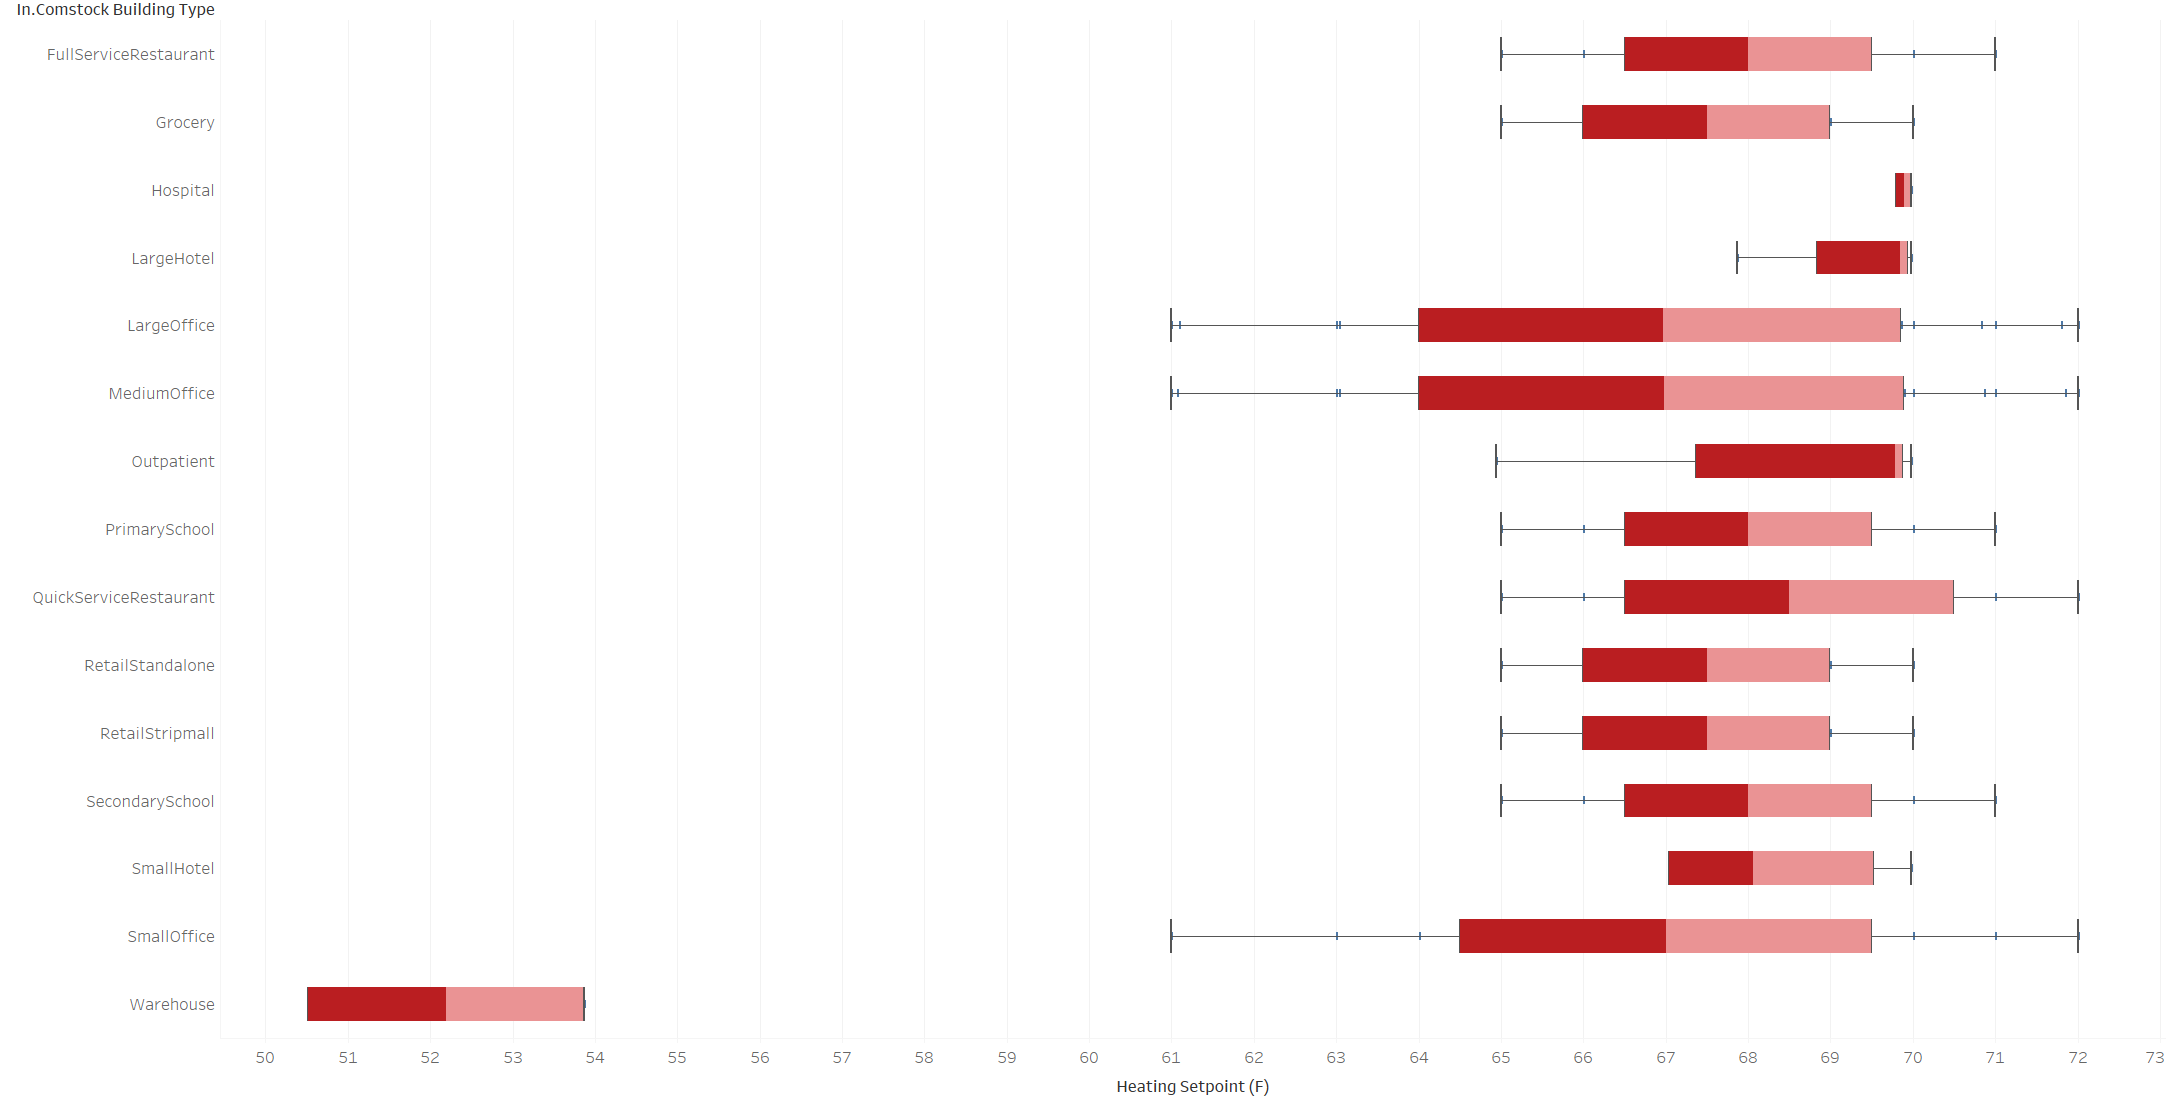
\includegraphics[width=1.0\textwidth]{figures/heating_setpoints.png}
    \caption{Heating thermostat set point (Fahrenheit) distributions per building type.}
    \label{fig:htg_therm_setpoints}
\end{figure}

\begin{figure}
    \centering 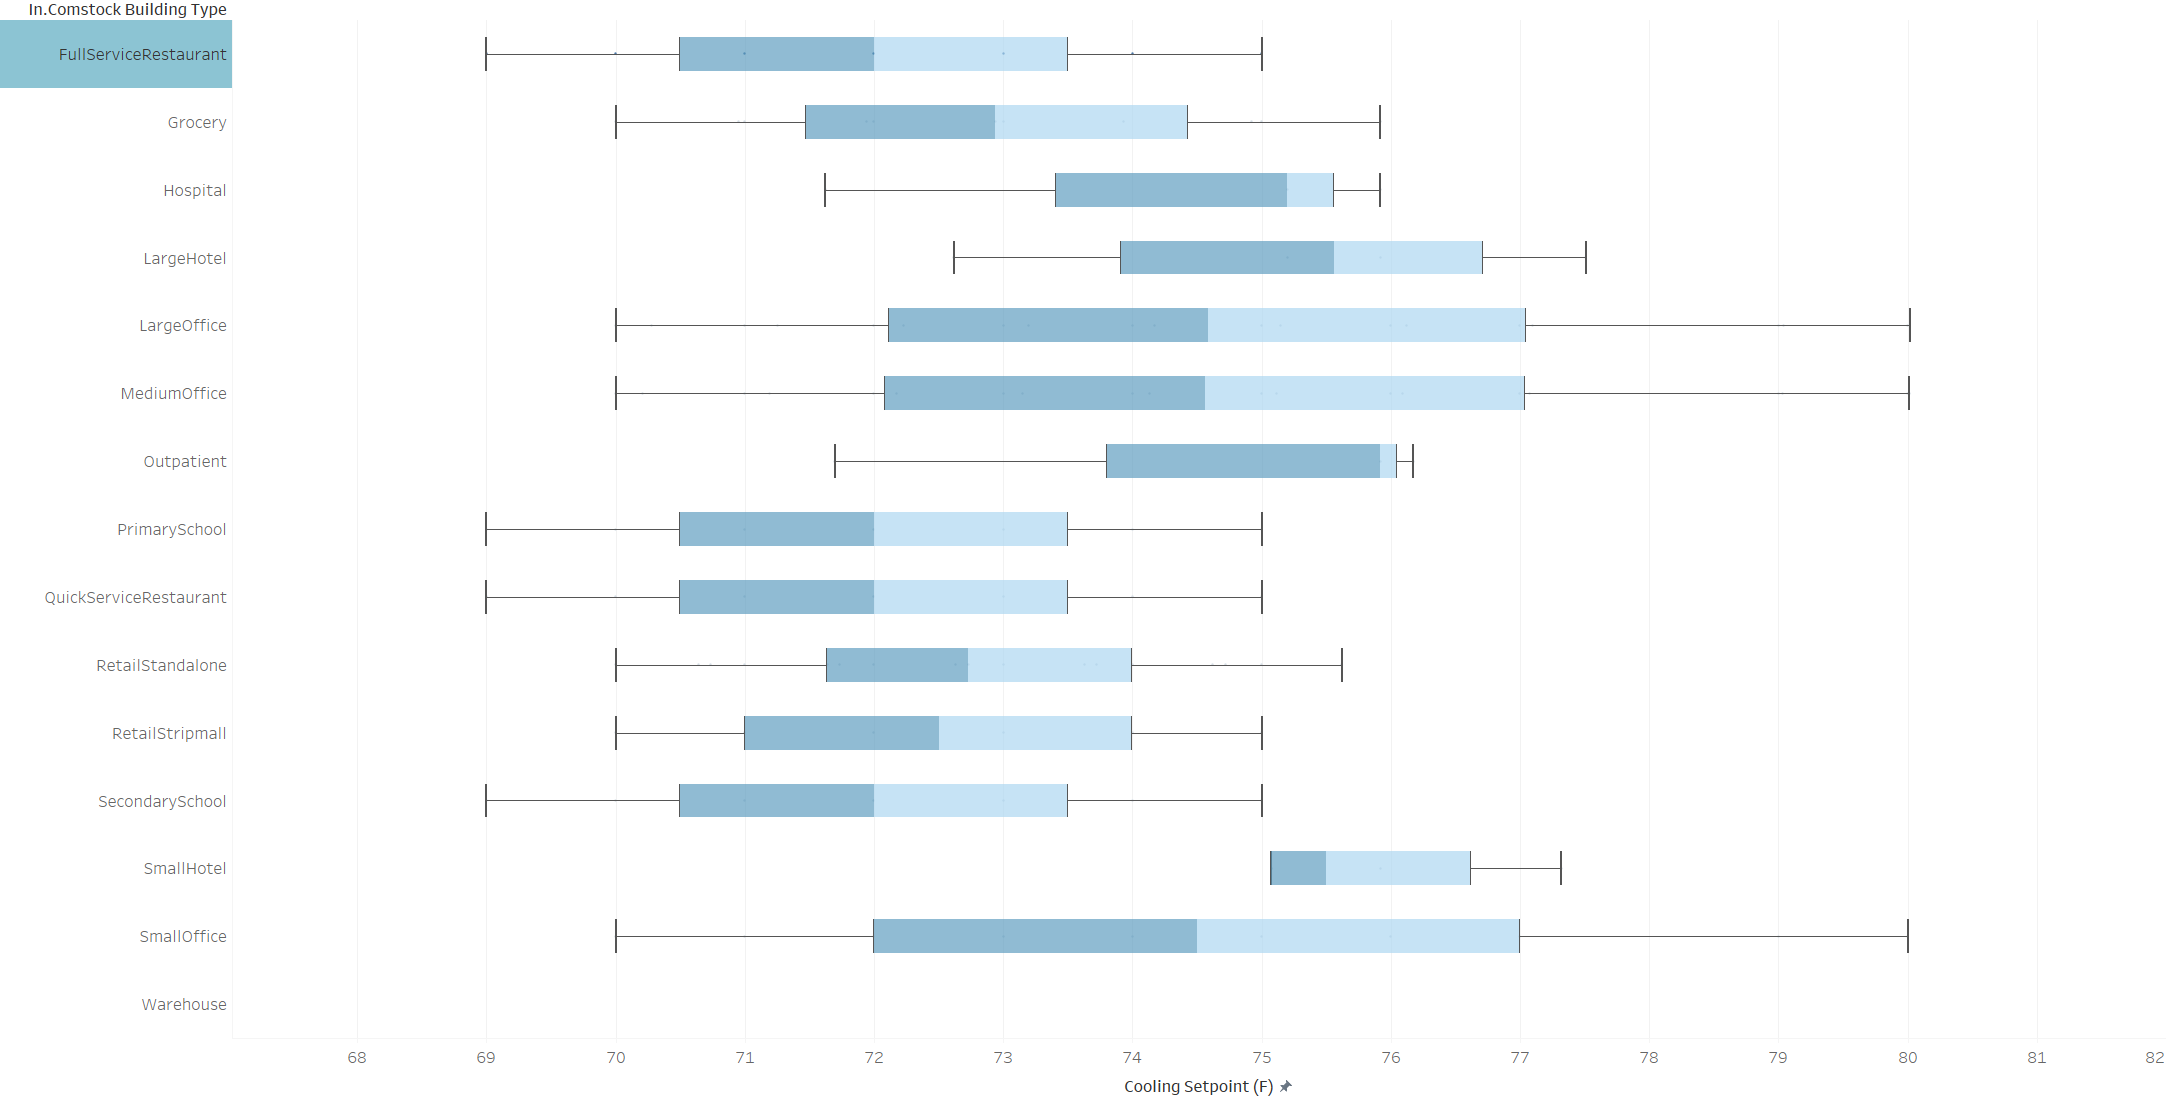
\includegraphics[width=1.0\textwidth]{figures/cooling_setpoints.png}
    \caption{Cooling thermostat set point (Fahrenheit) distributions per building type.}
    \label{fig:clg_therm_setpoints}
\end{figure}

\pagebreak
\subsubsection{Unoccupied Thermostat Setbacks}

An unoccupied thermostat setback defines the difference in the temperature set point from the occupied thermostat set point, for either heating or cooling, which is used during periods where the building is unoccupied. For example, an office might have an occupied heating set point of 71°F, but an unoccupied thermostat setback of 6°F for when the building is unoccupied, resulting in an unoccupied thermostat set point of 65°F (71°F - 6°F). This setback would be expected to save HVAC energy by relaxing the temperature requirements when there are no occupants in the building. This section describes ComStock's methodology for assigning unoccupied thermostat setback prevalence, as well as the setback temperature delta, for both heating and cooling.

The prevalence of thermostat setbacks in ComStock models is determined by building type using CBECS 2012. Each building type has some fraction of buildings with a thermostat setback, and some fraction without. The CBECS survey does not provide details on thermostat set point and setback temperatures, but it does provide survey responses as to whether heating and cooling setbacks are used, and whether these setbacks are manual. The survey responses are summarized by building type in Figure~\ref{fig:cbecs_therm_setback_summary}. However, it seems likely that many respondents who claim to implement manual setbacks do not reliably do so; we made a conservative assumption that only 20\% of manual setbacks would be counted as reliably practicing thermostat setbacks (manually adjusting the thermostat every night before leaving and every morning upon entering). The fraction of ComStock models that include thermostat setbacks is shown in Table~\ref{tab:thermostat_setback_prev}. Note that the timing of the thermostat setbacks coincides with the assigned hours of operation for a specific model, the methodology for which is described in Section~\ref{sec:hoo}.

\medskip
\begin{table}
\centering
\small
\caption[Fraction of ComStock Buildings with Thermostat Setbacks]{Fraction of ComStock Buildings With Thermostat Setbacks by Building Type}
\label{tab:thermostat_setback_prev}
\begin{tabular}{|l|l|}
\hline
\textbf{Building Type}          & \textbf{Fraction of Models With Thermostat Setback} \\ \hline
FullServiceRestaurant  & 0.57                                                \\ \hline
LargeOffice            & 0.77                                                \\ \hline
MediumOffice           & 0.76                                                \\ \hline
PrimarySchool          & 0.9                                                 \\ \hline
QuickServiceRestaurant & 0.46                                                \\ \hline
RetailStandalone       & 0.63                                                \\ \hline
RetailStripmall        & 0.9                                                 \\ \hline
SecondarySchool        & 0.95                                                \\ \hline
SmallOffice            & 0.77                                                \\ \hline
Warehouse              & 0.56                                                \\ \hline
\end{tabular}
\end{table}

\subsubsection{Unoccupied Thermostat Setbacks Informed by Building Automation System Data}

The method for determining the magnitude of the temperature setback for buildings with unoccupied temperature setbacks is described in this section. This methodology is used for the following building types: full service restaurant, large office, medium office, primary school, quick service restaurant, retail standalone, retail strip mall, secondary school, small office, and warehouse. In warehouse buildings, this methodology only applies to the office space type within the building.

The magnitudes of the temperature setbacks are determined using the same data sets and methods described in Section~\ref{section:therm_setpoints_bas} for thermostat set points; probability distributions are created for each building type. The relationship between the thermostat set points and the delta setbacks is shown in Figure~\ref{fig:therm_setpoint_setback}. The resulting heating and cooling thermostat delta setback temperature probability distributions, for each applicable building type, are shown in Figure~\ref{fig:therm_heating_setback} and Figure~\ref{fig:therm_cooling_setback}, respectively.

\begin{figure}
    \centering 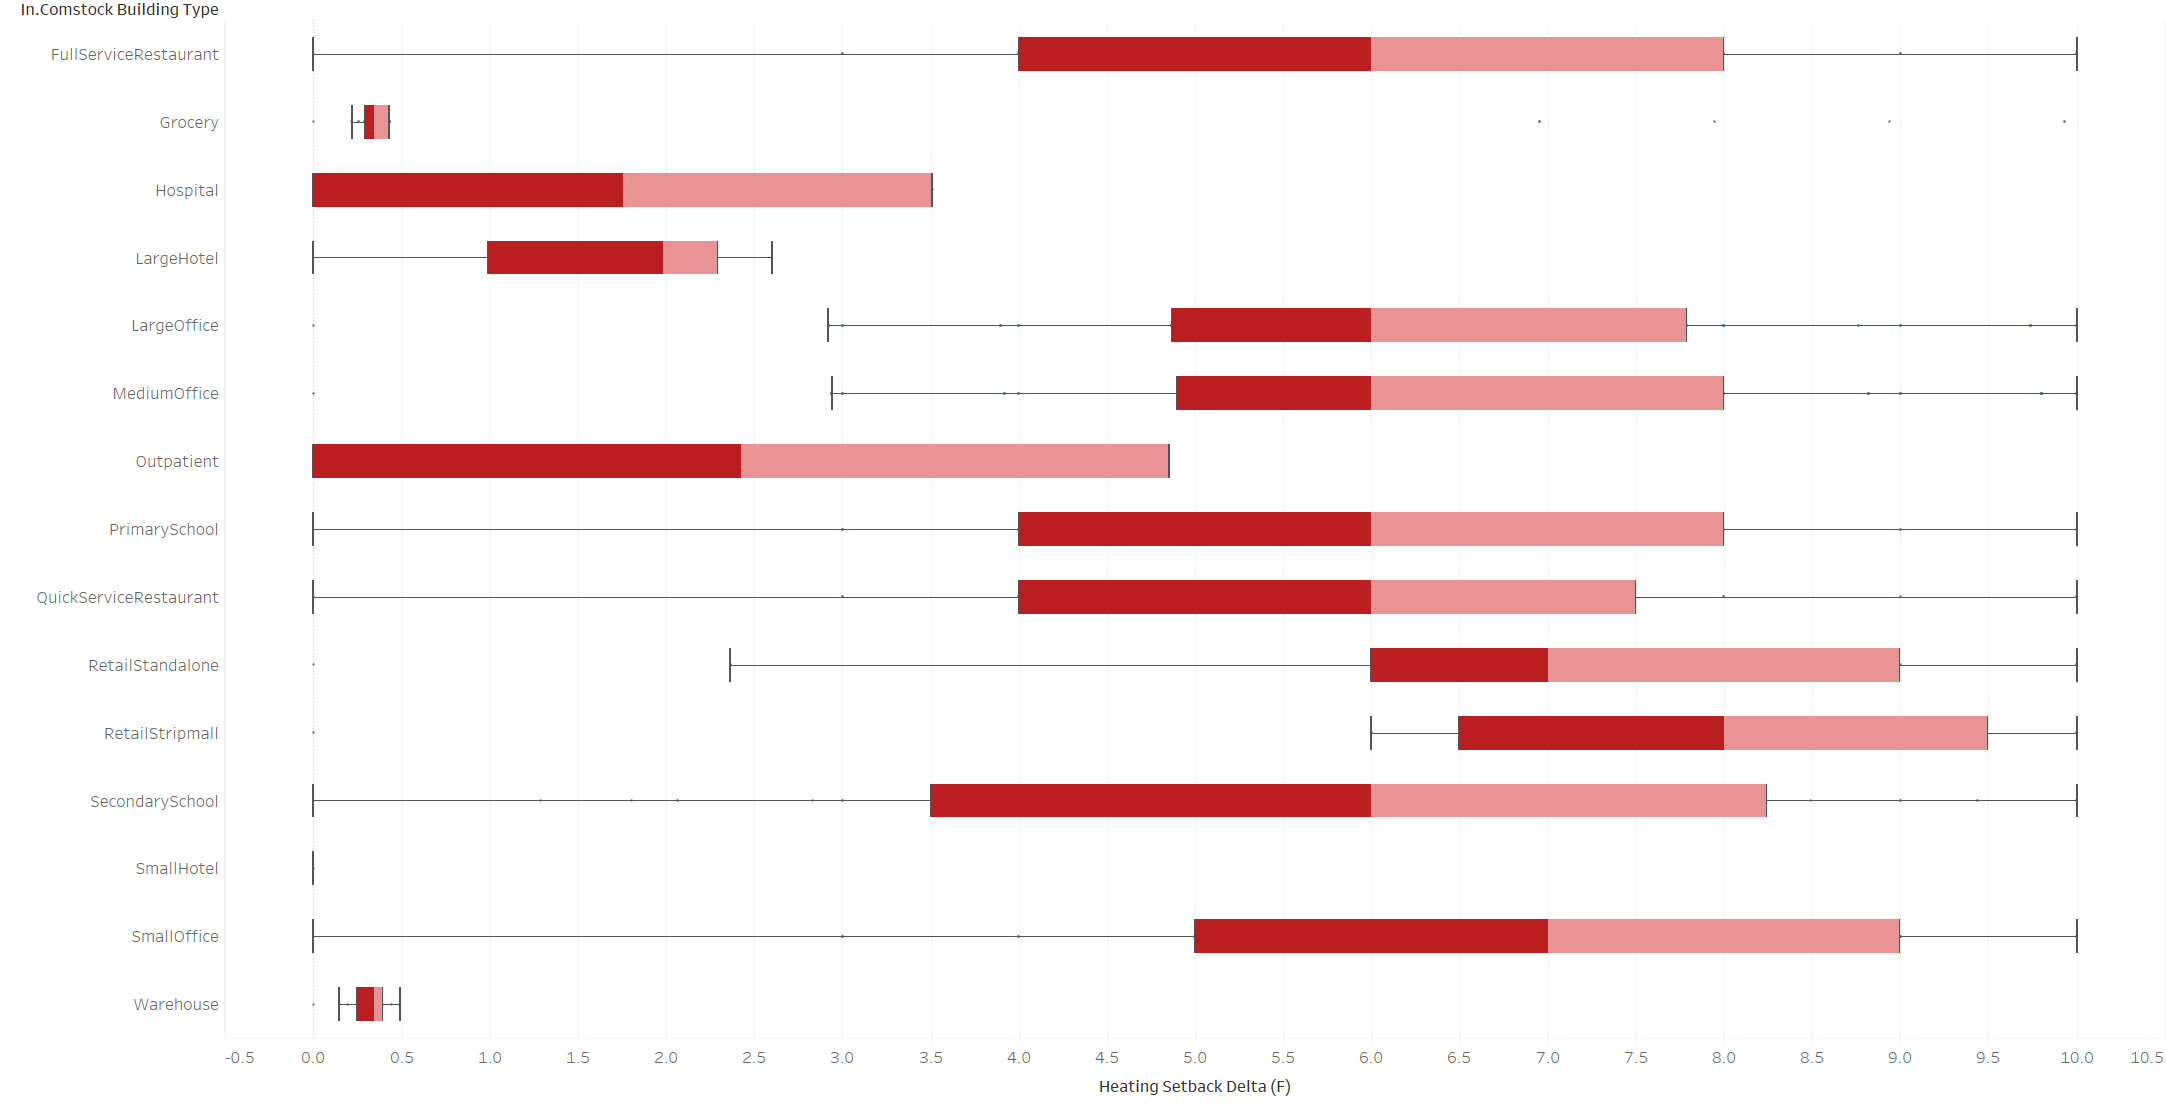
\includegraphics[width=1.0\textwidth]{figures/heating_setbacks.png}
    \caption{Thermostat heating setback delta temperature probability distributions per building type.}
    \label{fig:therm_heating_setback}
\end{figure}

\begin{figure}
    \centering 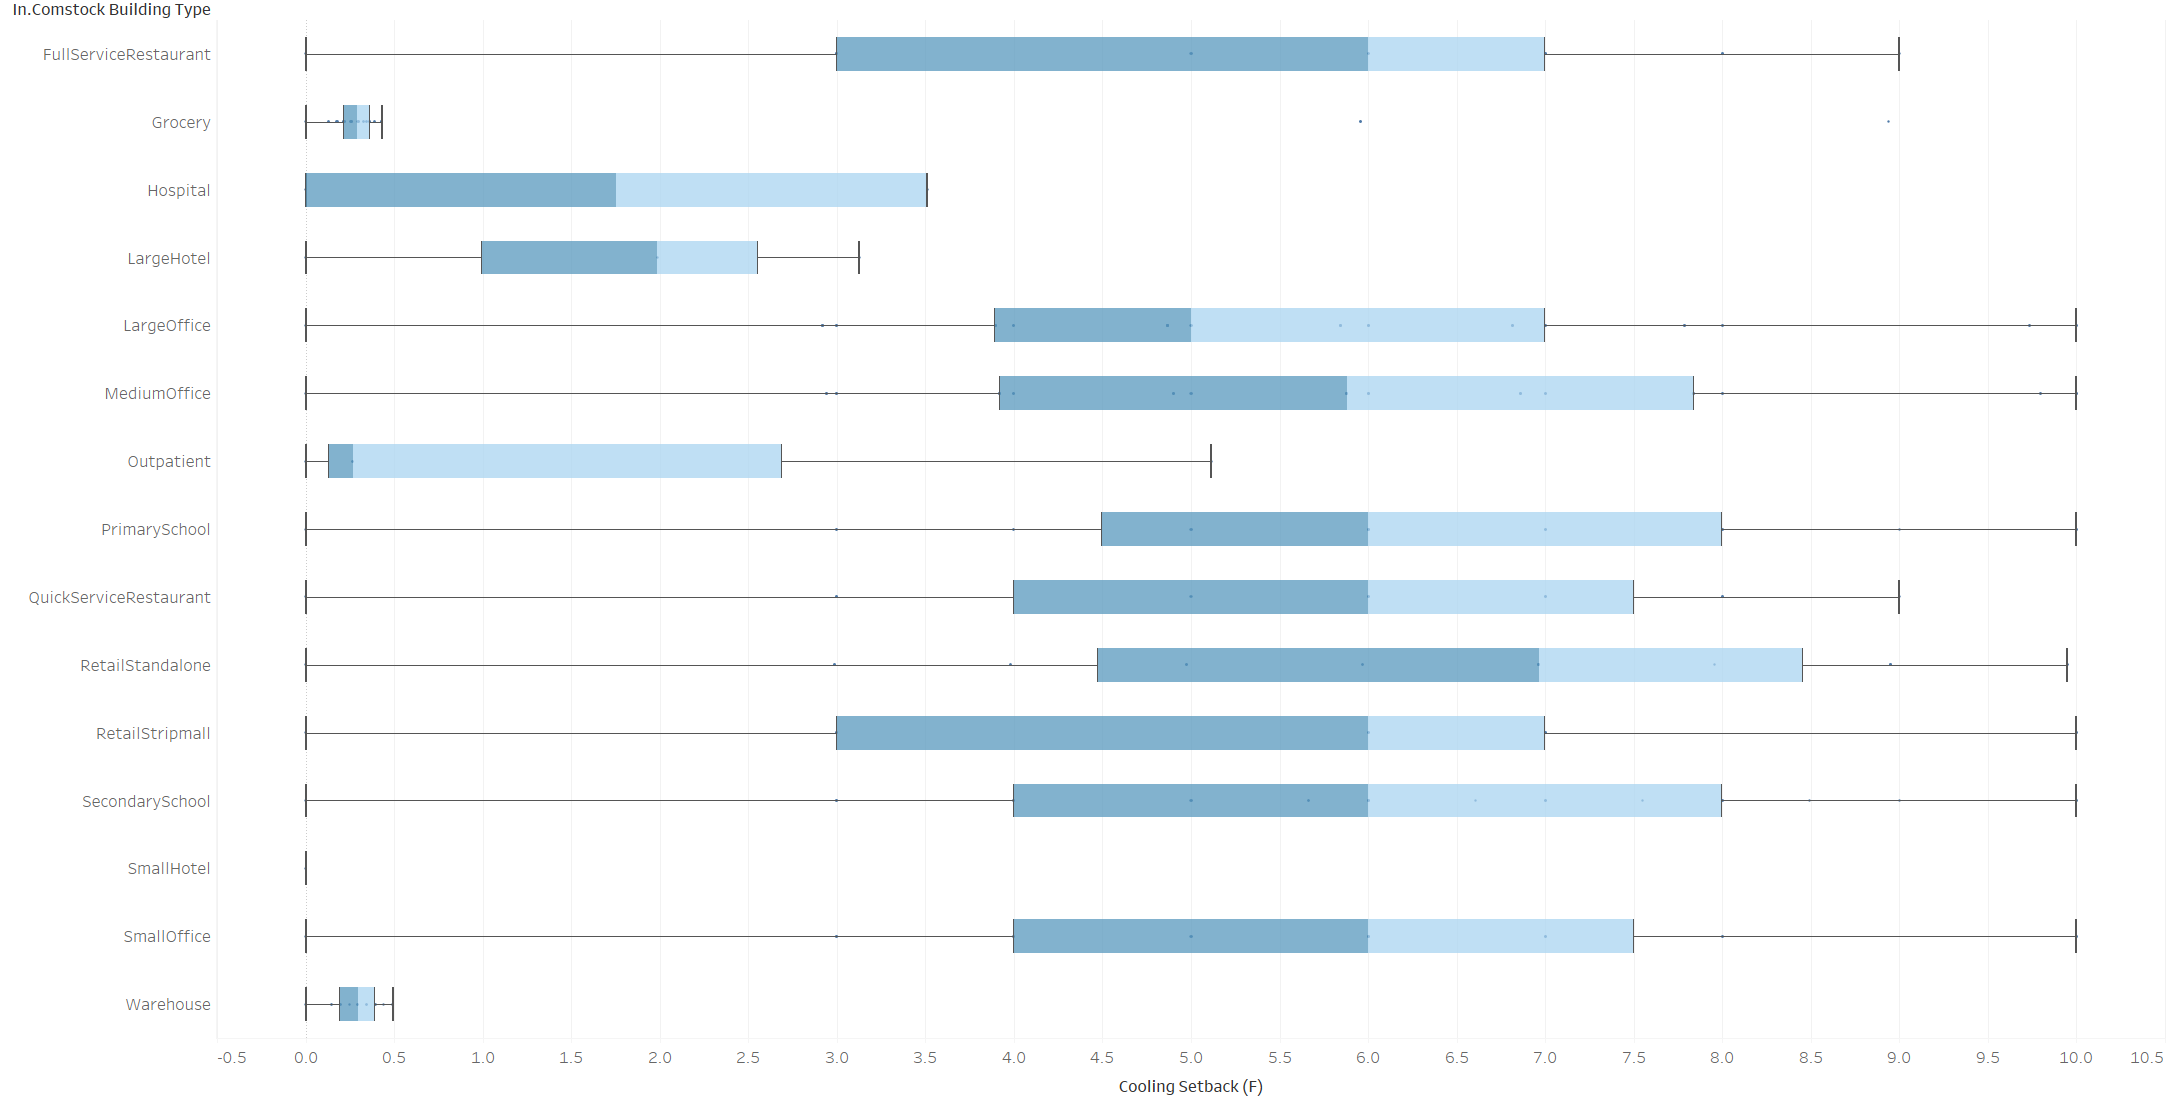
\includegraphics[width=1.0\textwidth]{figures/cooling_setbacks.png}
    \caption{Thermostat cooling setback delta temperature probability distributions per building type.}
    \label{fig:therm_cooling_setback}
\end{figure}

\subsubsection{Thermostat Setpoints Not Informed by Building Automation System Data}
% TODO: All of these alternative building types
The following ComStock building types do not infer thermostat setpoints from the BAS data, and therefore each have there own methodology previously described in this section: Hospitals, Outpatient, Warehouses, Small Hotels, and Large Hotels.
%\paragraph{Hospitals}
%\paragraph{Outpatient}
\paragraph{Warehouses}

Heating thermostat setpoints for warehouse storage spaces are adjusted from the DOE/DEER prototype model defaults in order to better calibrate warehouse energy consumption to the CBECS truth data set, informed by CBECS 2018 \citep{eia2018cbecs} responses to the ``Percent Heated'' and ``Percent Cooled'' questions as well as engineering judgement. The default DOE prototype setpoint value of 45°F (50°F for buildings built after 2004) was increased, and the default DEER prototype setpoint value of 70°F was decreased, both to a new heating setpoint of 61°F. Cooling thermostat setpoints remained unchanged, except for California (DEER prototype) warehousees, which are modeled as heated-only.

%\paragraph{Small Hotels}
%\paragraph{Large Hotels}

\pagebreak
\subsection{Unoccupied Air Handling Unit Operation}
\label{sec:unoccupied_ahu_operation}

Commercial buildings require constant design outdoor air ventilation rates when the building is occupied per ASHRAE-90.1. For air handling units (AHUs), the outdoor air is generally mixed with the supply air. This requires constant supply fan operation to maintain the outdoor air requirements established by ASHRAE-62.1 \citep{ashrae_62.1_2004}. However, AHUs do not need to provide outdoor ventilation air when the building is unoccupied. Therefore, ASHRAE-90.1 requires outdoor air dampers to close when the building is unoccupied, and to only cycle on supply fans as needed to maintain thermostat set points. This control scheme can have a large impact on energy usage, and data suggests that not all buildings implement these controls in their AHU systems. This section discusses ComStock's methodology for including the prevalence of different unoccupied AHU control schemes observed in real buildings, which follows the methodology used in \cite{unocc_hvac_paper}.

An industry-provided BAS data set of over 5,700 AHUs was used to inform the prevalence of three unoccupied AHU operation modes. The data set includes time series (hourly) BAS variables for ``Occupied Status'' (describes whether the AHU was in an occupied mode for that hour), ``Fan Status'' (describes whether the fan was used for that hour), and ``Ventilation Status'' (describes whether outdoor ventilation air was used for that hour). Counts of AHUs and buildings by building type in the data set are shown in Table~\ref{tab:unnoc_ahu_data_counts}, and the three unoccupied AHU shutdown control schemes are summarized in Table~\ref{tab:unnoc_ahu_schemes}.

The data set suggests that 27\% of AHUs use scheme 1 (least efficient), 50\% of AHUs use scheme 2 (more efficient), and 23\% of AHUs use scheme 3 (most efficient; ASHRAE-90.1 required). The prevalence of the AHU unoccupied control schemes by building type is shown in Table~\ref{tab:unnoc_ahu_scheme_prev}. These probability distributions are used in ComStock sampling to set the fraction of buildings utilizing the discussed control schemes, by building type, for models that use AHU-based HVAC systems. Non-AHU HVAC system types are not applicable to this methodology, nor are building types not listed in Table~\ref{tab:unnoc_ahu_scheme_prev}. Note that building types with less than 25 buildings in the BAS data set (Table~\ref{tab:unnoc_ahu_data_counts}) use the ``All Types'' distribution of the data set at large, as fewer than 25 samples cannot reliably be used to represent a population.

The following building types are not included in the unnocupied air handling unit operation workflow, and utilize default scheduling only: small hotels, large hotels, outpatient, hospitals, primary schools, and secondary schools. The building types may be integrated into this workflow in the future as more data becomes available.

\begin{table}[h!]
\centering
\small
\caption{Site and AHU Counts of Time Series BAS Data per Building Type}
\label{tab:unnoc_ahu_data_counts}
\begin{tabular}{|l|l|l|}
\hline
\textbf{Building Type} & \textbf{Site   Count} & \textbf{AHU   Count} \\ \hline
\textbf{All Types}     & 843                   & 5,706                \\ \hline
\textbf{Retail}        & 541                   & 3,300                \\ \hline
\textbf{Unknown}       & 164                   & 1,391                \\ \hline
\textbf{Office}        & 43                    & 466                  \\ \hline
\textbf{Restaurant}    & 39                    & 155                  \\ \hline
\textbf{Grocery}       & 35                    & 212                  \\ \hline
\textbf{Hotel}         & 6                     & 46                   \\ \hline
\textbf{Education}     & 6                     & 29                   \\ \hline
\textbf{Warehouse}     & 5                     & 94                   \\ \hline
\textbf{Healthcare}    & 4                     & 13                   \\ \hline
\end{tabular}
\end{table}
\begin{table}[h!]
\centering
\caption{AHU Operating Mode Schemes Used During Scheduled Unoccupied Times}
\label{tab:unnoc_ahu_schemes}
\begin{tabular}{|p{2.2cm}|p{4cm}|p{2cm}|p{2cm}|p{2cm}|p{2cm}|}
\hline
\textbf{Scheme Name} &
  \textbf{Unoccupied Control Scheme Description} &
  \textbf{Expected Efficiency} &
  \textbf{Occupied Status} &
  \textbf{Fan Status} &
  \textbf{Ventilation Status} \\ \hline
\textbf{Scheme 1} & Scheduled on, running                                                            & Least Efficient & Active   & Active & Active   \\ \hline
\textbf{Scheme 2} & Scheduled off, fan cycles with ventilation to maintain thermostat   setpoints    & More Efficient  & Inactive & Active & Active   \\ \hline
\textbf{Scheme 3} & Scheduled off, fan cycles without ventilation to maintain thermostat   setpoints & Most Efficient  & Inactive & Active & Inactive \\ \hline
\end{tabular}
\end{table}

\subsection{Demand Control Ventilation}

Demand control ventilation (DCV) acts to reduce outdoor air ventilation during periods of detected low occupancy. Occupancy levels are generally detected through the use of CO\textsubscript{2} sensors located directly in the space or within the HVAC system.

DCV is included in ComStock models when required by the governing ASHRAE-90.1 energy code for the specific spaces/systems in the model. ComStock gathers the necessary criteria for determining DCV requirements and includes DCV functionality only if the space/system requires it. The requirement criteria for DCV include space floor area, space design occupant density, system economizer prevalence, system design outdoor air flow rate, and system energy recovery prevalence. The 90.1 code year for a model is based on the year of the model's last major HVAC replacement. Code year assignment and system turnover assumptions are described further in Section \ref{sec:system_turnover_and_eul}. A summary of the floor area served by a system with DCV is shown in Table~\ref{tab:dcv_prev}. Note that DCV is not required by ASHRAE 90.1 when an HVAC system has an ERV. One important observation from these data is that no office buildings include DCV. This is because office buildings are currently modeled using a single, blended space type that is a fractional mix of open offices, enclosed offices, conference rooms, etc. The occupancy density of this blended space does not exceed the DCV thresholds in ASHRAE 90.1. This leads to unrealistically low (0\%) DCV in office buildings. Another important observation is that DCV is not modeled in any of the buildings in California (which use the DEER data set), although this does not align with the newer versions of Title 24. DCV is expected to be implemented in California buildings in the near future.
%NOTE: DCV table does not look good. Nothing for DEER. Inconsistent for code years. Nothing for offices.
%TODO: DIscuss DCV excemptions, such as ERV prev


\subsection{Air-Side Energy Recovery}
\label{sec:erv}

Energy recovery ventilators (ERVs) in AHUs reduce energy consumption by pre-conditioning the incoming outdoor air using the system exhaust air, which reduces the heating and cooling energy required to condition the air. Energy recovery is especially effective in systems serving spaces with high outdoor air ventilation loads.

ERVs are included in ComStock model HVAC systems only when required by the governing energy code for the specific system. This determination is made using OpenStudio-Standards, where the necessary ComStock model properties are gathered to determine whether an ERV is required for each system. These properties include the climate zone, percent outdoor air, and design supply airflow rate, aligning with ASHRAE-90.1 Table 6.5.6.1 for the respective energy code year followed. A summary of the floor area served by systems with energy recovery is shown in Table~\ref{tab:energy_recovery_prev}.

%TODO: Discuss ERV wheel power methodology

\begin{table}[h!]
\centering
\scriptsize
\caption[Energy Recovery Prevalence]{Fraction of Floor Area Served by HVAC Systems With Energy Recovery by Building Type and Code Year}
\label{tab:energy_recovery_prev}
\begin{tabular}{|p{2.2cm}|p{0.3in}|p{0.3in}|p{0.3in}|p{0.3in}|p{0.3in}|p{0.3in}|p{0.3in}|}
\hline
\textbf{Building Type} &
  \textbf{Pre-1980} &
  \textbf{1980--2004} &
  \textbf{90.1-2004} &
  \textbf{90.1-2007} &
  \textbf{90.1-2010} &
  \textbf{90.1-2013} &
  \textbf{DEER All Years} \\ \hline
FullService\-Restaurant  & 0 & 0 & 0.051 & 0.027 & 0.347 & 0.392 & 0 \\ \hline
Hospital               & 0 & 0 & 0.457 & 0.442 & 0.613 & 0.871 & 0 \\ \hline
LargeHotel             & 0 & 0 & 0.109 & 0.09  & 0.267 & 0.245 & 0 \\ \hline
LargeOffice            & 0 & 0 & 0.028 & 0.035 & 0.139 & 0.519 & 0 \\ \hline
MediumOffice           & 0 & 0 & 0.007 & 0.016 & 0.093 & 0.306 & 0 \\ \hline
Outpatient             & 0 & 0 & 0.087 & 0.078 & 0.095 & 0.246 & 0 \\ \hline
PrimarySchool          & 0 & 0 & 0.376 & 0.41  & 0.597 & 0.639 & 0 \\ \hline
QuickService\-Restaurant & 0 & 0 & 0     & 0     & 0.088 & 0.063 & 0 \\ \hline
RetailStandalone       & 0 & 0 & 0.027 & 0.022 & 0.029 & 0.306 & 0 \\ \hline
RetailStripmall        & 0 & 0 & 0.115 & 0.111 & 0.191 & 0.435 & 0 \\ \hline
SecondarySchool        & 0 & 0 & 0.540 & 0.530 & 0.675 & 0.725 & 0 \\ \hline
SmallHotel             & 0 & 0 & 0.186 & 0     & 0.092 & 0     & 0 \\ \hline
SmallOffice            & 0 & 0 & 0     & 0     & 0.044 & 0.050 & 0 \\ \hline
Warehouse              & 0 & 0 & 0.065 & 0.053 & 0.069 & 0.083 & 0 \\ \hline
\end{tabular}
\end{table}

An enthalpy wheel ERV system (rotary) is added to the HVAC systems in ComStock models where an ERV is determined to be required. The effectiveness of the system is 50\% for all conditions, aligning with the requirements of ASHRAE-90.1. Economizer lockout and supply air bypass for temperature control are included. The defrost type is exhaust only, which temporarily bypasses the supply side of the heat exchanger to allow warmer exhaust air to remove frost uninhibited when needed.

\subsection{Air-Side Economizers}

Air-side economizers reduce HVAC cooling energy by increasing the amount of outdoor ventilation air during times when the temperature and/or enthalpy are beneficial for cooling. For example, if the outdoor air temperature is 55°F when the building needs cooling, the HVAC system can increase the amount of outdoor ventilation air being delivered to the space to satisfy some or all of the cooling requirement in place of mechanical cooling.

As described in Section~\ref{sec:system_turnover_and_eul}, we assume that some building systems, including the HVAC system, are replaced over the lifespan of the building. We re-evaluate the requirement for an air-side economizer based on the energy code in force at the time of the latest HVAC system replacement. For buildings outside of CA, energy code requirements were taken from ASHRAE 90.1. For buildings inside CA, the CA energy code requirements were evaluated taken from the CA DEER MASControl3 models \citep{mascontrol3}, where the economizer limits and applicability were found as shown in Table~\ref{tab:econ_lims_mascontrol3} and Table~\ref{tab:econ_applic_mascontrol3}.

\begin{table}[h!]
  \centering
  \small
  \caption[MASControl3 Economizer Limits]{Economizer limits from MASControl3}
  \label{tab:econ_lims_mascontrol3}
  \begin{tabular}{|p{0.75in}|p{1.25in}|p{1.5in}|}
  \hline
  \textbf{Climate Zone} &
  \textbf{Drybulb Limit (°F)} &
  \textbf{Enthalpy Limit (Btu/lb)} \\ \hline
  CZ01 & 70 & 28 \\ \hline
  CZ02 & 73 & 28 \\ \hline
  CZ03 & 70 & 28 \\ \hline
  CZ04 & 73 & 28 \\ \hline
  CZ05 & 70 & 28 \\ \hline
  CZ06 & 71 & 28 \\ \hline
  CZ07 & 69 & 28 \\ \hline
  CZ08 & 71 & 28 \\ \hline
  CZ09 & 71 & 28 \\ \hline
  CZ10 & 73 & 28 \\ \hline
  CZ11 & 75 & 28 \\ \hline
  CZ12 & 75 & 28 \\ \hline
  CZ13 & 75 & 28 \\ \hline
  CZ14 & 75 & 28 \\ \hline
  CZ15 & 75 & 28 \\ \hline
  CZ16 & 75 & 28 \\ \hline
  \end{tabular}
  \end{table}

\begin{table}[h!]
  \centering
  \small
  \caption[MASControl3 Economizer Applicability]{Economizer applicability from MASControl3}
  \label{tab:econ_applic_mascontrol3}
  \begin{tabular}{|p{0.75in}|p{1in}|p{1in}|p{1in}|}
  \hline
  \textbf{Vintage} &
  \textbf{Packaged DX} &
  \textbf{Chilled Water} &
  \textbf{Water Loop HP} \\ \hline
  1975  & FALSE & TRUE & FALSE \\ \hline
  1985  & FALSE & TRUE & FALSE \\ \hline
  ~1996 & FALSE & TRUE & FALSE \\ \hline
  2003  & FALSE & TRUE & FALSE \\ \hline
  2007  & FALSE & TRUE & FALSE \\ \hline
  2011  & FALSE & TRUE & FALSE \\ \hline
  2014  & TRUE  & TRUE & TRUE  \\ \hline
  2015  & TRUE  & TRUE & TRUE  \\ \hline
  2017  & TRUE  & TRUE & TRUE  \\ \hline
  2020  & TRUE  & TRUE & TRUE  \\ \hline
  \end{tabular}
  \end{table}

Figure~\ref{fig:economizer_presence} shows the prevalence of economizers (in terms of floor area coverage and contribution to cooling energy) for different subcategories (building type and ventilation system type) of the existing building stock. The percentage of floor area where "economizer availability" is "True" includes the total building area if there is at least one economizer in the building. It does not represent the total floor area served by systems with economizers. While there are buildings that already include economizers in variable air volume (VAV) systems and roof top units (RTU) covering 40\% of the total floor area and 28\% of total electricity used for cooling, the remaining portion of buildings with those system types do not include economizers.

\begin{figure}
  \centering 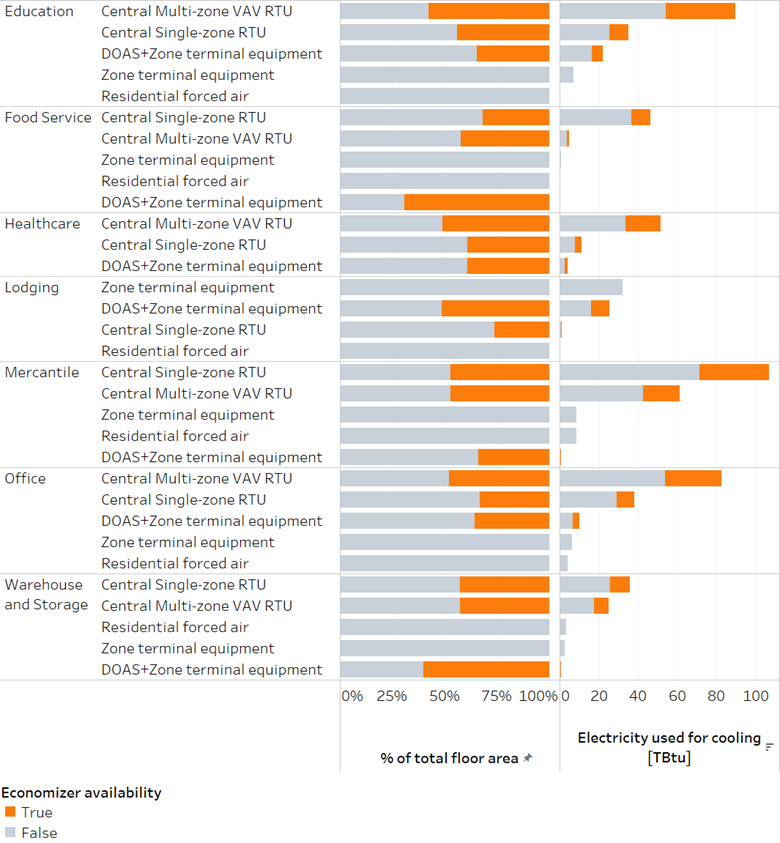
\includegraphics[width=0.7\textwidth]{figures/economizer_presence.png}
  \caption{Presence of air-side economizers in the building stock.}
  \label{fig:economizer_presence}
\end{figure}

Based on a large body of anecdotal evidence from conversations with fault-focused field engineers and a brief review of common current (Trane, Carrier, Daikin) rooftop unit product data sheets \citep{trane_foundation}, \citep{carrier_economiser}, \citep{daikin_rebel}, fixed dry bulb controls are a more common choice than differential dry bulb controls, although manufacturers also offer dual enthalpy (fixed dry bulb + fixed enthalpy) options with the addition of an enthalpy sensor. For this reason, fixed dry bulb controls are assumed for almost all building vintages and climate zones, with the exception being ASHRAE 90.1-2010 and 2013, which prohibited fixed dry bulb economizers in the warmer humid climate zones. These restrictions were lifted in ASHRAE 90.1-2016.

Figure~\ref{fig:economizer_prevalence} shows the comparison of economizer coverage with respect to building floor area between ComStock and estimation from Commercial Buildings Energy Consumption Survey \citep{eia2018cbecs}. Because of how data is structured in CBECS, the floor area shown in these figures represents the entire floor area of the building if any economizer is present in any of the HVAC systems in the building rather than actual floor area covered by HVAC systems with an economizer. Because CBECS data only shows total building area instead of total area covered by the economizers, this comparison helps give a rough estimate of economizers.

\begin{figure}
  \centering 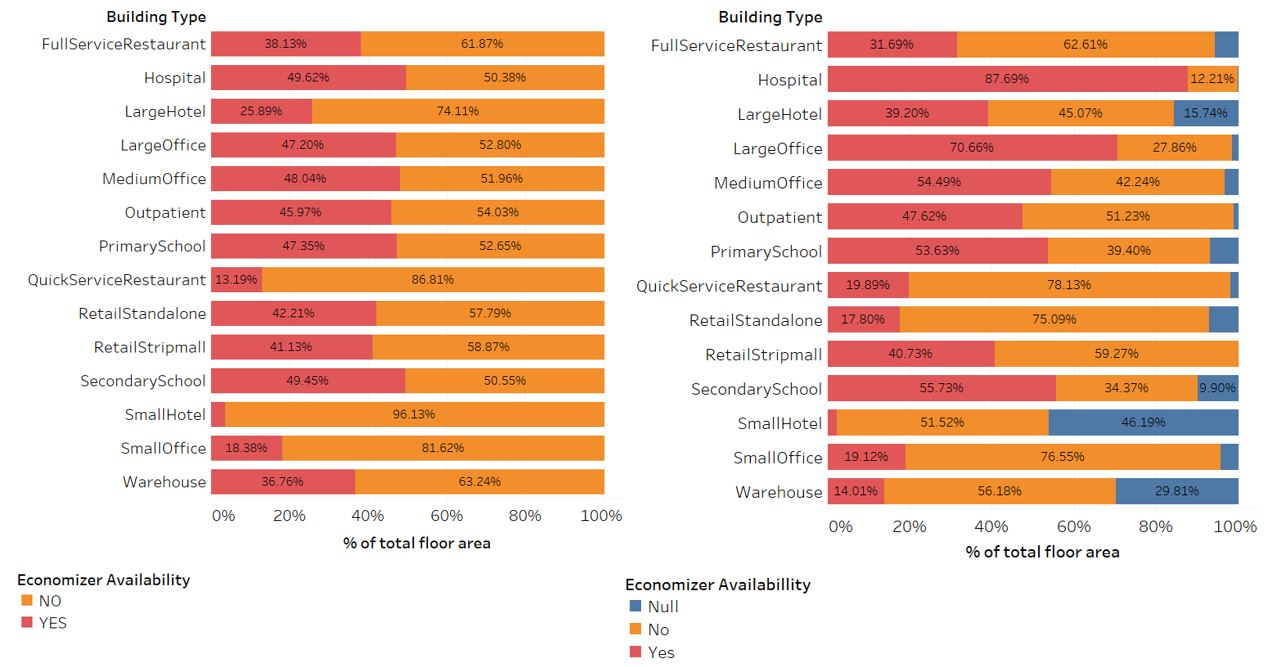
\includegraphics[width=0.7\textwidth]{figures/economizer_prevalence.png}
  \caption{Economizer floor area coverage comparing ComStock (left) with CBECS 2018 (right).}
  \label{fig:economizer_prevalence}
\end{figure}

Economizers are well known for frequent faulty operations. There were many efforts in the past to understand fault characteristics in commercial buildings \citep{doi_10_1080_23744731_2021_1898243}, \citep{osti_1889192}, \citep{osti_1829706}, \citep{osti_1457127}. While this evidence is insufficient to reflect all aspects (e.g., prevalence, incidence, intensity, and evolution described in \citep{doi_10_1080_23744731_2021_1898243}) of all faults in the commercial building stock across the country, it is possible to make simplifications for modeling certain fault types based on available data.

Figure~\ref{fig:econ_temp_fault} shows how the first fault is modeled for buildings with economizers. Crowe et al. \citep{osti_1889192} acquired data from AFDD venders that monitored 3,660 AHUs and 7,974 RTUs and reported 31\% of all economizers were experiencing faulty operations. Shoukas et al. \citep{osti_1665808} received data from a clothing retailer and food chain that monitored 1,416 RTUs and reported 60\% of all faults related to economizers were related to economizer not effectively reducing cooling load compared to the theoretical potential. The symptom described as "ineffective economizing" can be due to different faults: damper stuck, damper bias, sensor bias, sensor frozen, inappropriate configuration, etc. A report \citep{seventhwave_rtu} published by Minnesota Department of Commerce Division of Energy Resources monitored 41 RTUs in Minnesota that were installed in many different building types (e.g., office, restaurant, retail, hotel, etc.) and reported the actual changeover temperature setting in the economizer were not configured efficiently (average of 52°F) resulting in missed free cooling opportunity.

Based on this information focusing on different aspects of the fault, a fault measure was developed as shown in Figure~\ref{fig:econ_temp_fault}. The figure includes a description of the fault as well as four different metrics that define the characteristics of a fault. Fault intensity (or severity) is when a fault can have a severity level. For example, if the sensor is drifting, the intensity is the difference between the true value and the biased measured value. Fault prevalence refers to the portion of systems or components with the fault among all systems or components in the sample space (e.g., 30\% of all economizers have the fault). Fault incidence refers to the occurrence rate of a fault for a given system or component over for a given time period (e.g., economizer damper gets stuck once every year). Fault evolution refers to certain faults where the severity naturally changes over time. For example, sensor drift is typically a fault where the severity changes over the course of time. For the incorrect high limit setting described in Figure~\ref{fig:econ_temp_fault}, the fault changes the changeover temperature setting of an economizer to 52°F and applies to 30\% of economizers that use fixed dry-bulb control. Fault incidence and fault evolution were not modeled because these aspects are mostly irrelevant for this fault.

\begin{figure}
  \centering 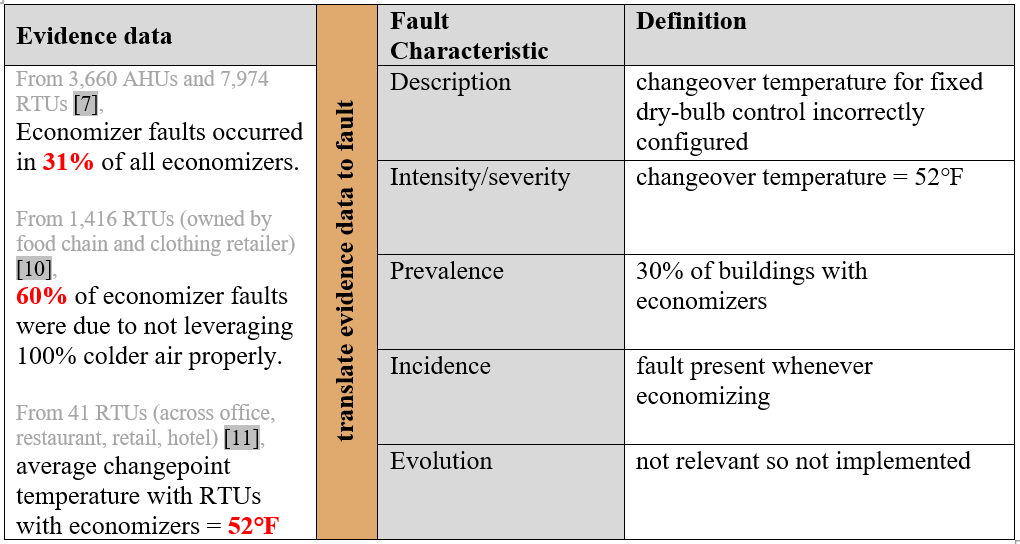
\includegraphics[width=0.7\textwidth]{figures/econ_temp_fault.png}
  \caption{Economizer incorrect changeover temperature setting fault description.}
  \label{fig:econ_temp_fault}
\end{figure}

Figure~\ref{fig:econ_temp_fault_single_model} shows a comparison of simulated operation with and without the fault. As a result, the fault will reduce the changeover (high limit) temperature of the economizer, disabling the economizer even if the outdoor air temperature is favorable (e.g., 52-72°F), thus, losing opportunities for free cooling. The figure shows how the fault impacts the annual cooling energy, how the changepoint temperature changes with fault, and how the transient response changes.

\begin{figure}
  \centering 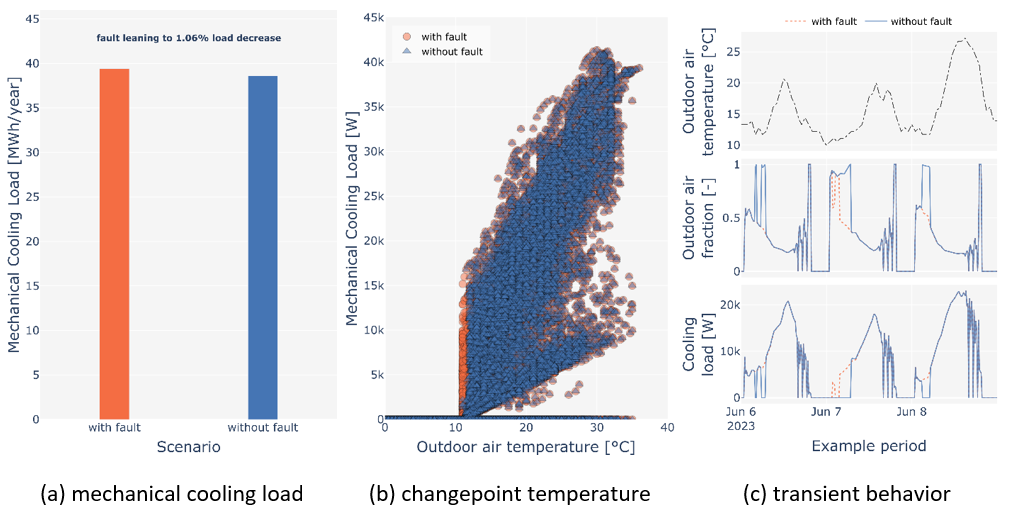
\includegraphics[width=0.7\textwidth]{figures/econ_temp_fault_single_model.png}
  \caption{Economizer incorrect changeover temperature setting fault impact on simulation results.}
  \label{fig:econ_temp_fault_single_model}
\end{figure}

As reported by Heinemeier \citep{heinemeier2014free}, contractors in California stated that 30-40\% of economizers they have worked with were disabled with fully closed dampers. This is often caused by mechanical linkage issues between damper and actuator, where the economizer automatically reverts to the fully closed position as a safety measure. An economizer with a fully closed damper will not draw any fresh outdoor air, causing an air quality issue. Depending on the outdoor air condition (i.e., favorable or not favorable for economizing), it can either reduce or increase energy consumption. Figure~\ref{fig:econ_damper_fault} shows the description of the fault for the economizer outdoor air damper fully closed and stuck. Unlike the fault described in Figure~\ref{fig:econ_temp_fault}, this fault has a bigger impact on air quality and energy and the incidence of the fault is important.

\begin{figure}
  \centering 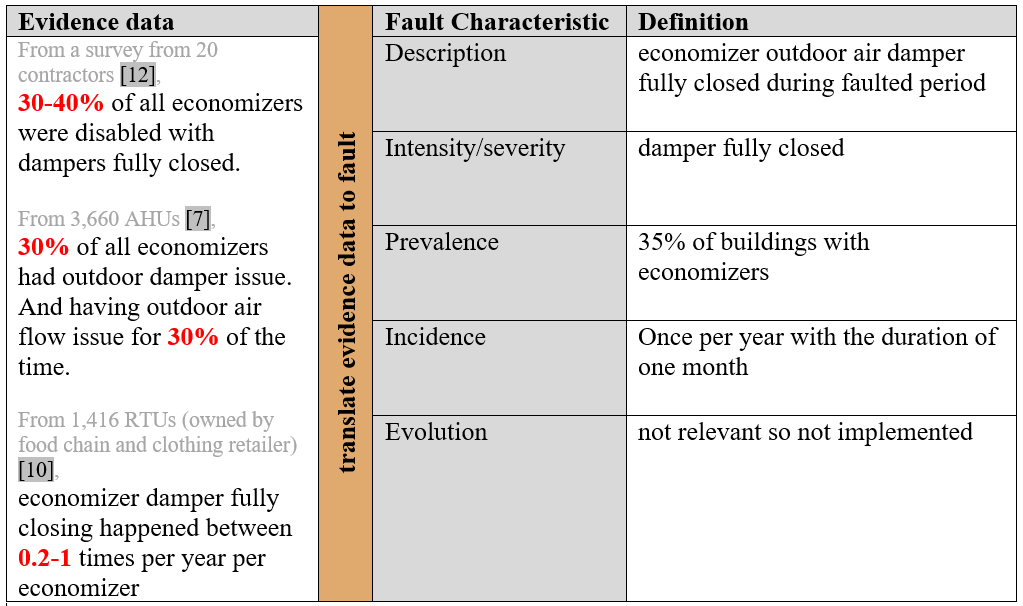
\includegraphics[width=0.7\textwidth]{figures/econ_damper_fault.png}
  \caption{Economizer damper stuck closed fault description.}
  \label{fig:econ_damper_fault}
\end{figure}

Figure~\ref{fig:econ_damper_fault_single_model} shows example simulation results for a building with and without the damper fully closed fault. The fault was imposed once during the entire April period resulting in 1.8\% mechanical load increase. As mentioned previously, the energy impact of the fault can either be increased or decreased energy consumption, and Figure~\ref{fig:econ_damper_fault_single_model}(c) highlights the transition from negative to positive savings when the outdoor air temperature transitions from favorable to unfavorable conditions.

\begin{figure}
  \centering \includegraphics[width=0.7\textwidth]{figures/econ_damper_fault_single_model.png}
  \caption{Economizer damper stuck closed fault impact on simulation results.}
  \label{fig:econ_damper_fault_single_model}
\end{figure}

Although faults (e.g., damper fully closed) are implemented with fixed prevalence (e.g., 35\%), the actual percentage of economizers being faulted (among applicable economizers) is less than the defined prevalence due to implementation limitations. For example, 35\% of randomly selected buildings that include certain HVAC system types (categorized by the air system) are assigned the damper fully closed fault. However, certain portions of these air systems do not have economizers, thus, they cannot have an economizer fault. In other words, the current limitation is that the random selection of faulted economizers is not fully aligned with buildings that actually have economizers. In these cases, we are losing the opportunity for applying faults and decreasing the representation of fault prevalence in final building stock. Newer versions of California's Title 24 energy code requires fault detection and diagnostics (FDD) for economizers which should prevent and mitigate faults. However, ComStock does not reflect the impact of FDD technology, possibly overestimating the impact of faults in buildings with newer HVAC systems in California.

\subsection{Furnaces}

Furnaces are used in a variety of HVAC equipment for space heating through the direct combustion of a fuel. For ComStock models, the fuel type can be natural gas, propane, or fuel oil. The following ComStock system types use furnaces: PSZ-AC with electric coil, PSZ-AC with gas coil, PTAC with electric coil, PTAC with gas coil, residential AC with residential forced air furnace, and residential forced air furnace.

\subsubsection{Furnace Efficiencies}

Furnaces in ComStock are all assumed to be standard, non-condensing types at this time. Rated efficiency assignments are a function of capacity and in-force HVAC template code. The furnace efficiency assignments are summarized in Table~\ref{tab:furnace_eff_assignments}.

\subsubsection{Furnace Performance Modifiers}

Furnaces in ComStock do not use any performance curves, so there is no change in efficiency or capacity as a function of temperature or part load ratio, and therefore no cycling losses. Furthermore, no parasitic fuel losses are included in ComStock furnace models.

\begin{table}
\centering
\scriptsize
\caption[Furnace Efficiency]{Furnace Efficiency by Capacity and Code Year}
\label{tab:furnace_eff_assignments}
\begin{tabular}{|p{0.5in}|p{0.5in}|p{0.5in}|p{0.5in}|p{0.5in}|p{0.5in}|p{1.5in}|}
\hline
\textbf{Template} &
  \textbf{Minimum   Capacity (Btu/hr)} &
  \textbf{Maximum   Capacity (Btu/hr)} &
  \textbf{Minimum   Annual Fuel Utilization Efficiency (AFUE)} &
  \textbf{Minimum   Thermal Efficiency (\%)} &
  \textbf{Minimum   Combustion Efficiency (\%)} &
  \textbf{Notes} \\ \hline
Pre-1980  & -           & 249,999       & -    & 0.8 & -   & -                                        \\ \hline
Pre-1980  & 250,000     & no max & -    & 0.8 & -   & -                                        \\ \hline
Pre-1980  & 250,000,000 & no max & -    & 0.8 & -   & -                                        \\ \hline
1980--2004 & -           & 299,999       & -    & 0.8 & -   & -                                        \\ \hline
1980--2004 & 300,000     & 249,999,999   & -    & 0.8 & -   & -                                        \\ \hline
90.1-2004           & -           & 224,999       & 0.78 & 0.8 & -   & \multirow{10}{*}{\parbox{2.5cm}{Table   6.8.1E page 49}} \\ \cline{1-6}
90.1-2004           & 225,000     & 249,999,999   & -    &     & 0.8 &                                          \\ \cline{1-6}
90.1-2007           & -           & 224,999       & 0.78 & 0.8 & -   &                                          \\ \cline{1-6}
90.1-2007           & 225,000     & 249,999,999   & -    &     & 0.8 &                                          \\ \cline{1-6}
90.1-2010           & -           & 224,999       & 0.78 & 0.8 & -   &                                          \\ \cline{1-6}
90.1-2010           & 225,000     & 249,999,999   & -    & 0.8 & -   &                                          \\ \cline{1-6}
90.1-2013           & -           & 224,999       & 0.78 & 0.8 & -   &                                          \\ \cline{1-6}
90.1-2013           & 225,000     & 249,999,999   & -    & 0.8 & -   &                                          \\ \cline{1-6}
90.1-2016           & -           & 224,999       & 0.78 & 0.8 & -   &                                          \\ \cline{1-6}
90.1-2016           & 225,000     & 249,999,999   & -    & 0.8 & -   &                                          \\ \hline
90.1-2019           &  -          & 224,999       & -    & 0.81 &
  - &
  \multirow{2}{*}{\parbox{1.5in}{Table   6.8.1-6 for \textgreater 225 kBtu/hr; Table F-4 for \textless 225 kBtu/hr}} \\ \cline{1-6}
90.1-2019           & 225,000     & 249,999,999   & -    & 0.8 & -   &                                          \\ \hline
\end{tabular}
\end{table}

\subsection{Boilers}

Boilers create hot water for heating in buildings. The following ComStock HVAC types use boilers for heating: DOAS with fan coil air-cooled chiller with boiler, DOAS with fan coil chiller with boiler, DOAS with water source heat pumps cooling tower with boiler, PSZ-AC with gas boiler, PTAC with gas boiler, PVAV with gas boiler reheat, VAV air-cooled chiller with gas boiler reheat, and VAV chiller with gas boiler reheat.

\subsubsection{Boiler Efficiencies}
At this time, boiler systems in ComStock are all gas-fired (or other combustible fuels) storage tank non-condensing units. A single boiler is used to meet the hot water load for the entire building. Rated efficiency assignments are a function of the HVAC code year and boiler capacity, mirroring the requirements of ASHRAE-90.1, and are summarized in Table~\ref{tab:boiler_eff_table}.

\subsubsection{Boiler Part Load Efficiencies}
Boiler efficiency at different part load conditions is modeled through an assigned efficiency as a function of a part load ratio (PLR) cubic curve. The output of this curve is multiplied by the full load rated efficiency, providing the effective efficiency of the boiler for each time step. The performance curve assignments for different boiler scenarios are summarized in Table~\ref{tab:boiler_eff_table}. The curve features are shown in Table~\ref{tab:boiler_plr_curve_table}, and the curves are illustrated in Figure~\ref{fig:blr_plr_curves}.

Table~\ref{tab:boiler_eff_table} shows the older DOE reference building templates using a constant efficiency curve for the boiler (``Boiler Constant Efficiency Curve''). Therefore, these boilers do not currently have efficiency modifications at different part load conditions. This likely underestimates cycling losses that boilers experience at lower PLRs, and may underestimate their gas usage. The 90.1 templates for 2004 through 2010 exclusively use a performance curve for boilers with no turndown controls (``Boiler With No Minimum Turndown''). This provides some efficiency loss, as PLR is reduced. For 90.1-2013 and beyond, performance curves for boilers with minimum turndowns (``Boiler With Minimum Turndown'') are added for larger boiler systems. This provides a slight performance improvement compared to boilers with no minimum turndown. All three curves are illustrated in Figure~\ref{fig:blr_plr_curves}.

%NOTE (From Chris): The curves here do not match the prototype building documentation. I do not know where the "from regression of prototype buildings" curves come from.

%NOTE (From Chris): Currently, the boiler curve assignments result in the oldest boilers having the least efficiency degradation at lower part load ratios. This is probably the opposite of what we want. Recommend finding bad performance curves for older boilers.


\subsubsection{Boiler Controls}

ComStock boilers use 180°F hot water loops with flow that leaves the set point modulated, meaning the boiler model internally varies the flow rate so that the temperature leaving the boiler matches a set point. The delta T of the loop is 20°F. %TODO: do we always use constant setpoint, or is outdoor air reset included sometimes?

\begin{table}[htbp]
\centering
\scriptsize
\caption{Boiler Efficiency and Performance Curve Assignment}
\label{tab:boiler_eff_table}
\begin{tabular}{|p{0.5in}|p{0.5in}|p{1.7cm}|p{0.5in}|p{0.5in}|p{0.5in}|p{1in}|p{0.5in}|}
\hline
\textbf{Template} &
  \textbf{Minimum   Capacity (Btu/hr)} &
  \textbf{Maximum   Capacity (Btu/hr)} &
  \textbf{Minimum   Annual Fuel Utilization Efficiency (AFUE)} &
  \textbf{Minimum   Thermal Efficiency (\%)} &
  \textbf{Minimum   Combustion Efficiency (\%)} &
  \textbf{Efficiency Function of Part Load Ratio (EFFFPLR)} &
  \textbf{Notes} \\ \hline
Pre-1980 &
  - &
  299,999 &
   &
  0.73 &
   &
  \multirow{5}{*}{\parbox{0.5in}{Boiler Constant Efficiency Curve}} &
  \multirow{3}{*}{\parbox{0.5in}{From DOE Reference Buildings}} \\ \cline{1-6}
Pre-1980  & 300,000     & no max &      & 0.74 &      &                                                     &                                   \\ \cline{1-6}
Pre-1980  & 250,000,000 & 249,999,999 &      & 0.76 &      &                                                     &                                   \\ \cline{1-6} \cline{8-8} 
1980--2004 & -           & 299,999       & 0.8  &      &      &                                                     & \multirow{2}{*}{\parbox{0.5in}{From   90.1-1989}} \\ \cline{1-6}
1980--2004 & 300,000     & 249,999,999   &      &      & 0.8  &                                                     &                                   \\ \hline
90.1-2004           & -           & 299,999       & 0.8  &      &      & \multirow{11}{*}{\parbox{1in}{Boiler with No Minimum Turndown}} & \multirow{3}{*}{\parbox{0.5in}{From   90.1-2004}} \\ \cline{1-6}
90.1-2004           & 300,000     & 249,999,999   &      & 0.75 &      &                                                     &                                   \\ \cline{1-6}
90.1-2004           & 250,000,000 & no max &      &      & 0.8  &                                                     &                                   \\ \cline{1-6} \cline{8-8} 
90.1-2007           & -           & 299,999       & 0.8  &      &      &                                                     & \multirow{3}{*}{\parbox{0.5in}{From   90.1-2007}} \\ \cline{1-6}
90.1-2007           & 300,000     & 249,999,999   &      & 0.8  &      &                                                     &                                   \\ \cline{1-6}
90.1-2007           & 250,000,000 & no max &      &      & 0.82 &                                                     &                                   \\ \cline{1-6} \cline{8-8} 
90.1-2010           & -           & 299,999       & 0.8  &      &      &                                                     & \multirow{3}{*}{\parbox{0.5in}{From   90.1-2010}} \\ \cline{1-6}
90.1-2010           & 300,000     & 249,999,999   &      & 0.8  &      &                                                     &                                   \\ \cline{1-6}
90.1-2010           & 250,000,000 & no max &      &      & 0.82 &                                                     &                                   \\ \cline{1-6} \cline{8-8} 
90.1-2013           & -           & 299,999       & 0.82 &      &      &                                                     & \multirow{8}{*}{\parbox{0.5in}{From   90.1-2013}} \\ \cline{1-6}
90.1-2013           & 300,000     & 999,999       &      & 0.8  &      &                                                     &                                   \\ \cline{1-7}
90.1-2013           & 1,000,000   & 249,999,999   &      & 0.8  &      & \multirow{2}{*}{\parbox{1in}{Boiler with Minimum Turndown}}     &                                   \\ \cline{1-6}
90.1-2013           & 250,000,000 & no max &      &      & 0.82 &                                                     &                                   \\ \cline{1-7}
90.1-2016           & -           & 299,999       & 0.82 &      &      & \multirow{2}{*}{\parbox{1in}{Boiler with No Minimum Turndown}}  & \multirow{4}{*}{\parbox{0.5in}{From   90.1-2016}} \\ \cline{1-6}
90.1-2016           & 300,000     & 999,999       &      & 0.8  &      &                                                     &                                   \\ \cline{1-7}
90.1-2016           & 1,000,000   & 249,999,999   &      & 0.8  &      & \multirow{2}{*}{\parbox{1in}{Boiler with Minimum Turndown}}     &                                   \\ \cline{1-6}
90.1-2016           & 250,000,000 & no max &      &      & 0.82 &                                                     &                                   \\ \hline
90.1-2019           & -           & 299,999       & 0.84 &      &      & \multirow{2}{*}{\parbox{1in}{Boiler with No Minimum Turndown}}  & \multirow{4}{*}{\parbox{0.5in}{From   90.1-2019}} \\ \cline{1-6}
90.1-2019           & 300,000     & 999,999       &      & 0.8  &      &                                                     &                                   \\ \cline{1-7}
90.1-2019           & 1,000,000   & 249,999,999   &      & 0.8  &      & \multirow{2}{*}{\parbox{1in}{Boiler with Minimum Turndown}}     &                                   \\ \cline{1-6}
90.1-2019           & 250,000,000 & no max &      &      & 0.82 &                                                     &                                   \\ \hline
\end{tabular}
\end{table}

\subsection{Direct Expansion Cooling}

Standard air-cooled direct expansion (DX) cooling is the most prevalent cooling equipment type in commercial buildings. The following ComStock HVAC system types use DX cooling: PSZ-AC with district hot water, PSZ-AC with electric coil, PSZ-AC with gas boiler, PSZ-AC with gas coil, PSZ-HP, PTAC with electric coil, PTAC with gas boiler, PTAC with gas coil, PTHP
PVAV with PFP boxes, PVAV with district hot water reheat, PVAV with gas boiler reheat, PVAV with gas heat with electric reheat, residential AC with residential forced air furnace.

\subsubsection{DX Cooling Rated Performance}

DX cooling systems are assigned full load and part load efficiencies based on the HVAC code template for the model and the capacity. These assignments are summarized in Table\ref{tab:unitary_dx_efficiencies} (unitary DX) and Table\ref{tab:ptac_efficiencies} (PTAC). These values mirror those found in ASHRAE-90.1 (or those used in the DOE reference buildings for the pre-1980 template).


\subsubsection{DX Cooling Performance Modifiers}

The performance of DX cooling equipment changes based on operating conditions. ComStock DX cooling equipment uses five performance modifier curves to model this behavior. Energy input ratio (EIR) as a function of part load ratio (PLR) describes how the equipment efficiency varies at different load fractions, accounting for equipment cycling (Figure  \ref{fig:dx_eirfplr}). EIR as a function of temperature describes how the equipment efficiency varies based on both the outdoor air dry bulb temperature and the wet bulb temperature of the air entering the cooling coil (Figure \ref{fig:dx_eirft}). EIR as a function of airflow describes how the equipment efficiency varies as a function of the supply airflow fraction (Figure \ref{fig:dx_eirff}). Capacity as a function of temperature describes how the equipment available capacity varies as a function of both the outdoor air dry bulb temperature and the wet bulb temperature of the air entering the cooling coil (Figure \ref{fig:dx_capft}). Lastly, capacity as a function of airflow describes how the equipment available capacity varies as a function of the supply airflow fraction (Figure \ref{fig:dx_capff}). The outputs of the EIR modifiers are multiplied against the nominal EIR at every time step (except for the PLR modifier, which is divided), which provides the effective EIR at each time step. Meanwhile, the outputs of the two capacity modifiers are multiplied against the nominal capacity at every time step, yielding the effective available capacity for the time step.


\subsection{Air-Source Heat Pumps}

Air-source heat pumps (ASHPs) provide electric heating using a reverse vapor compression cycle. This generally provides a higher COP option for electric heating compared to standard electric resistance electric heating. In most cases, ASHPs use the same air-cooled DX system for both DX heating and DX cooling. ASHPs can be split system, packaged units, or through-the-wall packaged terminal heat pumps (PTHP). The following ComStock HVAC systems types use ASHPs: packaged single zone heat pump (PSZ-HP) and PTHP.

ASHP sizing is often based on the design cooling requirements. Because the DX cooling and heating use the same compressor system, the capacities for each are coupled. ASHPs generally have a minimum operating temperature, below which the DX heating is disabled due to lack of capacity and efficiency. To remedy this, backup heating is often included in colder climates, and for any system where the design heating load is higher than the design cooling load. ComStock ASHP sizing follows this methodology: ASHPs are sized to meet the design cooling load, and backup electric heating is added to the system to meet the design heating load when the available DX heating capacity is unavailable or insufficient. The minimum temperature for compressor operation for ComStock heat pump systems is 17°F PTHP and 10°F for PSZ-HP.
\begin{table}[h!]
\scriptsize
\centering
\caption{Air-Source Heat Pump Efficiency and Performance Curve Assignment}
\label{tab:ashp_eff}
\begin{tabular}{|p{0.4in}|p{0.5in}|p{0.75in}|p{0.4in}|p{0.4in}|p{0.4in}|p{0.4in}|p{0.4in}|p{0.4in}|}
\hline
\textbf{Template} &
  \textbf{Cooling Type} &
  \textbf{Subcategory} &
  \textbf{Minimum Capacity (Btu/hr)} &
  \textbf{Maximum Capacity (Btu/hr)} &
  \textbf{HSPF} &
  \textbf{Min COP} &
  \textbf{PTHP\_COP\_Coefficient\_1} &
  \textbf{PTHP\_COP\_Coefficient\_2} \\ \hline
\multirow{5}{*}{\parbox{0.4in}{\textbf{Pre-1980 Through 1980--2004}}} 
& AirCooled, ThroughWall    & Split System                  &  0      & 64,999    & 6.8 & & & \\ \cline{2-9}
& AirCooled                 & Single Package                & 0       & 64,999    & 6.6 & & & \\ \cline{2-9} 
& AirCooled                 & Single Package                & 65,000  & 134,999   &     & 3.2 & & \\ \cline{2-9} 
& AirCooled                 & Single Package                & 135,000 & no max    &     & 3.1 &     & \\ \cline{2-9} 
& AirCooled                 & PTHP                          & 0       & no max    &     &     & 2.9 & 0.026 \\ \hline
\multirow{5}{*}{\textbf{90.1-2004}}
& AirCooled, ThroughWall    & Split System                  & 0       & 64,999    & 6.8 &     &     & \\ \cline{2-9} 
& AirCooled, ThroughWall    & Single Package                & 0       & 64,999    & 6.6 &     &     & \\ \cline{2-9} 
& AirCooled                 & Single Package                & 65,000  & 134,999   &     & 3.2 &     & \\ \cline{2-9} 
& AirCooled                 & Single Package                & 135,000 & no max    &     & 3.1 &     & \\ \cline{2-9} 
& AirCooled                 & PTHP                          & 0       & no max    &     &     & 3.2 & 0.026 \\ \hline
\multirow{6}{*}{\textbf{90.1-2007}}
& ThroughWall               & Split System                  & 0       & 29,999    & 7.1 & & & \\ \cline{2-9} 
& AirCooled                 & Split System, Single Package  & 0       & 64,999    & 7.7 &     &     & \\ \cline{2-9} 
& ThroughWall               & Single Package                & 0       & 29,999    & 7   &     &     & \\ \cline{2-9} 
& AirCooled                 & Single Package                & 65,000  & 134,999   &     & 3.2 &     & \\ \cline{2-9} 
& AirCooled                 & Single Package                & 135,000 & no max    &     & 3.1 &     & \\ \cline{2-9} 
& AirCooled                 & PTHP                          & 0       & no max    &     &     & 3.2 & 0.026 \\ \hline
\multirow{5}{*}{\textbf{90.1-2010}} 
& ThroughWall               & Split System, Single Package  & 0 & 29,999 & 7.4 & & & \\ \cline{2-9} 
& AirCooled                 & Split System, Single Package  & 0       & 64,999    & 7.7 &     &     & \\ \cline{2-9} 
& AirCooled                 & Single Package                & 65,000  & 134,999   &     & 3.3 &     & \\ \cline{2-9} 
& AirCooled                 & Single Package                & 135,000 & no max    &     & 3.2 &     & \\ \cline{2-9} 
& AirCooled                 & PTHP                          & 0       & no max    &     &     & 3.2 & 0.026 \\ \hline
\multirow{6}{*}{\textbf{90.1-2013}} & ThroughWall & Split   System, Single Package & 0       & 29,999    & 7.4 &     &     &       \\ \cline{2-9} 
                                    & AirCooled   & Split   System                 & 0       & 64,999    & 8.2 &     &     &       \\ \cline{2-9} 
                                    & AirCooled   & Single   Package               & 0       & 64,999    & 8   &     &     &       \\ \cline{2-9} 
                                    & AirCooled   & Single   Package               & 65,000  & 134,999   &     & 3.3 &     &       \\ \cline{2-9} 
                                    & AirCooled   & Single   Package               & 135,000 & no max    &     & 3.2 &     &       \\ \cline{2-9} 
                                    & AirCooled   & PTHP                           & 0       & no max    &     &     & 3.7 & 0.052 \\ \hline
\multirow{6}{*}{\textbf{90.1-2016}} & ThroughWall & Split   System, Single Package & 0       & 29,999    & 7.4 &     &     &       \\ \cline{2-9} 
                                    & AirCooled   & Split   System                 & 0       & 64,999    & 8.2 &     &     &       \\ \cline{2-9} 
                                    & AirCooled   & Single   Package               & 0       & 64,999    & 8   &     &     &       \\ \cline{2-9} 
                                    & AirCooled   & Single   Package               & 65,000  & 134,999   &     & 3.3 &     &       \\ \cline{2-9} 
                                    & AirCooled   & Single   Package               & 135,000 & no max    &     & 3.2 &     &       \\ \cline{2-9} 
                                    & AirCooled   & PTHP                           & 0       & no max    &     &     & 3.7 & 0.052 \\ \hline
\multirow{8}{*}{\textbf{90.1-2019}} & ThroughWall & Split   System, Single Package & 0       & 29,999    & 7.4 &     &     &       \\ \cline{2-9} 
                                    & AirCooled   & Split   System                 & 0       & 64,999    & 8.2 &     &     &       \\ \cline{2-9} 
                                    & AirCooled   & Single   Package               & 0       & 64,999    & 8   &     &     &       \\ \cline{2-9} 
                                    & AirCooled   & Single   Package               & 65,000  & 134,999   &     & 3.3 &     &       \\ \cline{2-9} 
                                    & AirCooled   & Single   Package               & 135,000 & no max    &     & 3.2 &     &       \\ \cline{2-9} 
                                    & AirCooled   & PTHP                           & 0       & 6,999     &     & 3.3 &     &       \\ \cline{2-9} 
                                    & AirCooled   & PTHP                           & 6,999   & 14,999    &     &     & 3.7 & 0.052 \\ \cline{2-9} 
                                    & AirCooled   & PTHP                           & 14,999  & no max    &     & 2.9 &     &       \\ \hline
\end{tabular}
\end{table}

\subsubsection{ASHP Rated Performance}

ASHPs in ComStock are assigned efficiencies based on ASHRAE-90.1. The assigned efficiencies are based on the template code year, the unit capacity, and the unit type. These assignments are summarized in Table~\ref{tab:ashp_eff}.

\subsubsection{ASHP Performance Modifiers}

Similar to DX cooling equipment, the performance of ASHP equipment changes based on different operating conditions. The curve assignments are shown in Table~\ref{tab:ashp_curves}. ComStock ASHP equipment uses five performance modifier curves to model this behavior. Energy input ratio (EIR) as a function of part load ratio (PLR) describes how the equipment efficiency varies at different load fractions, where the nominal EIR is divided by the output of this curve to account for equipment cycling losses (Figure~\ref{fig:ashp_eirfplr}). EIR as a function of temperature describes how the equipment efficiency varies based on outdoor air dry bulb temperature (Figure~\ref{fig:ashp_eirft}). Figure~\ref{fig:ashp_eirft} illustrates the capacity loss of ASHPs at lower outdoor air temperatures. EIR as a function of airflow describes how the equipment efficiency varies as a function of the supply airflow fraction (Figure~\ref{fig:ashp_eirff}). Capacity as a function of temperature describes how the equipment available capacity varies as a function of outdoor air dry bulb temperature (Figure~\ref{fig:ashp_capff}). Lastly, capacity as a function of airflow describes how the equipment EIR ratio varies as a function of the supply airflow fraction (Figure~\ref{fig:ashp_capff}). The outputs of the EIR modifiers are multiplied against the nominal EIR at every time step (except for the PLR curve output, which is divided), which provides the effective EIR at each time step. Meanwhile, the outputs of the two capacity modifiers are multiplied against the nominal capacity at every time step, yielding the effective available capacity for the time step. The curves described here are primarily derived from the DOE prototype/reference building models.


\subsection{Air-Cooled Chillers}

Air-cooled chillers (ACCs) provide chilled water for building cooling systems and use an air-cooled condenser for heat rejection. Therefore, no condenser water loop is required for ACCs. The following ComStock HVAC types use ACCs: DOAS with fan coil air-cooled chiller with boiler, VAV air-cooled chiller with PFP boxes, VAV air-cooled chiller with district hot water reheat, and VAV air-cooled chiller with gas boiler reheat.

%TODO CHRIS: add in loop temperatures and setpoint managers.
%TODO CHRIS: chiller condenser type fixed in Standards. Update documentation. This removes the scroll chiller curves.

\subsubsection{Air-Cooled Chiller Rated Performance}

ACCs are assigned full load and part load efficiencies based on the HVAC code template for the model and the capacity. These assignments are summarized in Table~\ref{tab:acc_efficiencies}. These values mirror those found in ASHRAE-90.1 (or those used in the DOE reference buildings for the pre-1980 template).

\begin{table}
\scriptsize
\centering
\caption{Air-Cooled Chiller Efficiency and Performance Curve Assignment}
\label{tab:acc_efficiencies}
\begin{tabular}{|p{0.6in}|p{0.4in}|p{0.4in}|p{0.4in}|p{0.4in}|p{0.6in}|p{0.6in}|p{0.6in}|p{0.6in}|}
\hline
\textbf{Model Template} &
  \textbf{Minimum Capacity (Tons)} &
  \textbf{Maximum Capacity (Tons)} &
  \textbf{Minimum Full   Load Efficiency (kW/ton)} &
  \textbf{Minimum   Integrated Part Load Value (kW/ton)} &
  \textbf{Capacity Function of Temperature (Schedule Name)} &
  \textbf{EIR Function of Temperature  (Schedule Name)} &
  \textbf{EIR Function of PLR (Schedule Name)} &
  \textbf{Notes} \\ \hline
Pre-1980 & 0 & 149.99 & 1.303 & - &
  \multirow{4}{*}{\parbox{0.6in}{ChlrAir\_RecipQRatio\_fTchwsToadbSI}} &
  \multirow{4}{*}{\parbox{0.6in}{ChlrAir\_RecipEIRRatio\_fTchwsToadbSI}} &
  \multirow{4}{*}{\parbox{0.6in}{ChlrAir\_RecipEIRRatio\_fQRatio}} & From   90.1-1989 \\ \cline{1-5} \cline{9-9} 
Pre-1980  & 150 & 299.99   & 1.332 & -     &  &  &  & \multirow{3}{*}{\parbox{0.6in}{From DOE Reference Buildings}} \\ \cline{1-5}
Pre-1980  & 300 & no max   & 1.332 & -     &  &  &  &                                               \\ \cline{1-5}
1980-2004 & 150 & no max   & 1.407 & 1.407 &  &  &  &                                               \\ \hline
90.1-2004 &  0 & no max    & 1.256 & 1.153 &
  \multirow{4}{*}{\parbox{0.6in}{AirCooled\_Chiller\_2010\_PathA\_CAPFT}} &
  \multirow{4}{*}{\parbox{0.6in}{AirCooled\_Chiller\_2010\_PathA\_EIRFT}} &
  \multirow{4}{*}{\parbox{0.6in}{AirCooled\_Chiller\_AllCapacities\_2004\_2010\_EIRFPLR}} &
  \multirow{4}{*}{\parbox{0.6in}{From 90.1-2004 Table 6.8.1A}} \\ \cline{1-5}
90.1-2007         & 0   & no max   & 1.29  & 1.164 &  &  &  &                                               \\ \cline{1-5}
90.1-2010         & 0   & 149.99   & 1.255 & 0.941 &  &  &  &                                               \\ \cline{1-5}
90.1-2010         & 150 & no max   & 1.255 & 0.941 &  &  &  &                                               \\ \hline
90.1-2013         & 0   & 149.99   & 1.25  & 0.96 &
  \multirow{8}{*}{\parbox{0.6in}{ChlrAir\_ScrollQRatio\_fTchwsToadbSI}} &
  \multirow{8}{*}{\parbox{0.6in}{ChlrAir\_ScrollEIRRatio\_fTchwsToadbSI}} &
  \multirow{8}{*}{\parbox{0.6in}{ChlrAir\_ScrollEIRRatio\_fQRatio}} &
  \multirow{8}{*}{\parbox{0.6in}{Path A Efficiencies}} \\ \cline{1-5}
90.1-2013         & 150 & no max   & 1.25  & 0.94  &  &  &  &                                               \\ \cline{1-5}
90.1-2013         & 0   & 149.99 & 1.188 & 0.876 &  &  &  &                                               \\ \cline{1-5}
90.1-2013         & 150 & no max   & 1.188 & 0.857 &  &  &  &                                               \\ \cline{1-5}
90.1-2016         & 0   & 149.99 & 1.188 & 0.876 &  &  &  &                                               \\ \cline{1-5}
90.1-2016         & 150 & no max   & 1.188 & 0.857 &  &  &  &                                               \\ \cline{1-5}
90.1-2019         & 0   & 149.99 & 1.188 & 0.876 &  &  &  &                                               \\ \cline{1-5}
90.1-2019         & 150 & no max   & 1.188 & 0.857 &  &  &  &                                               \\ \hline
\end{tabular}
\end{table}

\subsubsection{Air-Cooled Chiller Performance Modifiers}

ACCs vary in capacity and efficiency under different operating conditions. ComStock uses three curve types to model the variation in performance: capacity as a function of temperature (CAPFT) modifier, EIR as a function of temperature (EIRFT) modifier, and EIR as a function of part load ratio (EIRFPLR) modifier. For each time step, the EIR modifier function outputs are multiplied by the ACC's rated EIR (except for the PLR curve output, which is divided). This provides the realized EIR for the time step. Similarly, the CAPFT modifier function output is multiplied by the ACC's nominal capacity every time step to get the actual available capacity for that time step. The curve assignments are summarized in Table \ref{tab:acc_efficiencies}, and the curve parameters are specified in Table \ref{tab:acc_perf_curves}. The curves are also illustrated in Figure \ref{fig:acc_eir_curves}, Figure \ref{fig:AirCooledChiller2010PathA_funct_curves}, and Figure \ref{fig:ChlrAirRecipQRatio_curves}.

%TODO, BUG: Standards does not specify the "condenser_type" field, so the model chooses the first in the list for the template call. This is why 2013 and beyond models use different performance curves.

\subsection{Water-Cooled Chillers}

Water-cooled chillers (WCCs) provide chilled water for building cooling systems and use a water-cooled condenser for heat rejection. Therefore, a condenser water loop is required for WCCs, generally conditioned by a boiler and cooling tower. The following ComStock HVAC types use WCCs: DOAS with fan coil chiller with baseboard electric, DOAS with fan coil chiller with boiler, DOAS with fan coil chiller with district hot water, VAV chiller with PFP boxes, VAV chiller with district hot water reheat, and VAV chiller with gas boiler reheat.

\subsubsection{Water-Cooled Chiller Rated Performance}

WCCs are assigned full load and part load efficiencies based on the HVAC code template for the model and the capacity. These assignments are summarized in Table~\ref{tab:wcc_eff}. These values mirror those found in ASHRAE-90.1 (or those used in the DOE reference buildings for the pre-1980 template).

\begin{table}
\scriptsize
\centering
\caption{Water-Cooled Chiller Efficiency and Performance Curve Assignment}
\label{tab:wcc_eff}
\begin{tabular}{|p{0.5in}|p{0.5in}|p{0.4in}|p{0.4in}|p{0.4in}|p{0.4in}|p{0.5in}|p{0.5in}|p{0.5in}|p{0.4in}|}
\hline
\textbf{Model Template} &
  \textbf{Compressor Type} &
  \textbf{Minimum Capacity (Tons)} &
  \textbf{Maximum Capacity (Tons)} &
  \textbf{Minimum Full Load Efficiency (kW/ton)} &
  \textbf{Minimum Integrated Part Load Value (kW/ton)} &
  \textbf{Capacity Function of Temperature (Schedule Name)} &
  \textbf{EIR Function of Temperature (Schedule Name)} &
  \textbf{EIR Function of PLR (Schedule Name)} &
  \textbf{Notes} \\ \hline
Pre-1980 &
  \multirow{32}{*}{\parbox{0.5in}{Rotary   Screw}} &
  0 & 149.99 & 0.852 & - &
  \multirow{9}{*}{\parbox{0.5in}{ChlrWtr\-PosDispPath\-AAll\-QRatio\-fTchws\-TcwsSI}} &
  \multirow{9}{*}{\parbox{0.5in}{ChlrWtr\-PosDispPath\-AAll\-EIRRatio\_fTchwsTcwsSI}} &
  \multirow{32}{*}{\parbox{0.5in}{ChlrWtr\-PosDispPath\-AAll\-EIRRatio\_fQRatio}} &
  \multirow{3}{*}{\parbox{0.5in}{From   DOE Reference Buildings}} \\ \cline{1-1} \cline{3-6}
Pre-1980  &  & 150 & 299.99 & 0.782 & -     &  &  &  &                                        \\ \cline{1-1} \cline{3-6}
Pre-1980  &  & 300 & no max   & 0.688 & -     &  &  &  &                                        \\ \cline{1-1} \cline{3-6} \cline{10-10} 
1980--2004 &  & 0   & 149.99 & 0.926 & 0.902 &  &  &  & \multirow{3}{*}{\parbox{0.5in}{From   90.1-1989}}      \\ \cline{1-1} \cline{3-6}
1980--2004 &  & 150 & 299.99 & 0.837 & 0.782 &  &  &  &                                        \\ \cline{1-1} \cline{3-6}
1980--2004 &  & 300 & no max   & 0.676 & 0.664 &  &  &  &                                        \\ \cline{1-1} \cline{3-6} \cline{10-10} 
90.1-2004 &  & 0   & 149.99 & 0.79  & 0.676 &  &  &  & \multirow{3}{*}{\parbox{0.5in}{Path   A Efficiencies}} \\ \cline{1-1} \cline{3-6}
90.1-2004 &  & 150 & 299.99 & 0.718 & 0.628 &  &  &  &                                        \\ \cline{1-1} \cline{3-6}
90.1-2004 &  & 300 & no max   & 0.639 & 0.572 &  &  &  &                                        \\ \cline{1-1} \cline{3-8} \cline{10-10} 
90.1-2007 &  & 0 & 74.99 & 0.78 & 0.63 &
  \multirow{8}{*}{\parbox{0.5in}{WaterCooled\_PositiveDisplacement\_Chiller\_LT150\_2010\_PathA\_CAPFT}} &
  \multirow{8}{*}{\parbox{0.5in}{WaterCooled\_PositiveDisplacement\_Chiller\_LT150\_2010\_PathA\_EIRFT}} &
   &
  \multirow{8}{*}{\parbox{0.5in}{Path   A Minimum Efficiencies}} \\ \cline{1-1} \cline{3-6}
90.1-2007           &  & 75  & 149.99 & 0.775 & 0.615 &  &  &  &                                        \\ \cline{1-1} \cline{3-6}
90.1-2007           &  & 150 & 299.99 & 0.68  & 0.58  &  &  &  &                                        \\ \cline{1-1} \cline{3-6}
90.1-2007           &  & 300 & no max   & 0.62  & 0.54  &  &  &  &                                        \\ \cline{1-1} \cline{3-6}
90.1-2010           &  & 0   & 74.99  & 0.78  & 0.63  &  &  &  &                                        \\ \cline{1-1} \cline{3-6}
90.1-2010           &  & 75  & 149.99 & 0.775 & 0.615 &  &  &  &                                        \\ \cline{1-1} \cline{3-6}
90.1-2010           &  & 150 & 299.99 & 0.68  & 0.58  &  &  &  &                                        \\ \cline{1-1} \cline{3-6}
90.1-2010           &  & 300 & no max   & 0.62  & 0.54  &  &  &  &                                        \\ \cline{1-1} \cline{3-8} \cline{10-10}
90.1-2013 & &
  0 & 74.99 & 0.75 & 0.6 &
  \multirow{15}{*}{\parbox{0.5in}{ChlrWtr\-PosDisp\-PathAAll\-QRatio\-fTchws\-TcwsSI}} &
  \multirow{15}{*}{\parbox{0.5in}{ChlrWtr\-PosDisp\-PathAAll\-EIRRatio\-fTchws\-TcwsSI}} & &
  \multirow{15}{*}{\parbox{0.5in}{Path   A Efficiencies}} \\ \cline{1-1} \cline{3-6}
90.1-2013 &  & 75  & 149.99 & 0.72 & 0.56 &  &  &  &  \\ \cline{1-1} \cline{3-6}
90.1-2013 &  & 150 & 299.99 & 0.66 & 0.54 &  &  &  &  \\ \cline{1-1} \cline{3-6}
90.1-2013 &  & 300 & 599.99 & 0.61 & 0.52 &  &  &  &  \\ \cline{1-1} \cline{3-6}
90.1-2013 &  & 600 & no max   & 0.56 & 0.5  &  &  &  &  \\ \cline{1-1} \cline{3-6}
90.1-2016 &  & 0   & 74.99  & 0.75 & 0.6  &  &  &  &  \\ \cline{1-1} \cline{3-6}
90.1-2016 &  & 75  & 149.99 & 0.72 & 0.56 &  &  &  &  \\ \cline{1-1} \cline{3-6}
90.1-2016 &  & 150 & 299.99 & 0.66 & 0.54 &  &  &  &  \\ \cline{1-1} \cline{3-6}
90.1-2016 &  & 300 & 599.99 & 0.61 & 0.52 &  &  &  &  \\ \cline{1-1} \cline{3-6}
90.1-2016 &  & 600 & no max   & 0.56 & 0.5  &  &  &  &  \\ \cline{1-1} \cline{3-6}
90.1-2019 &  & 0   & 74.99  & 0.75 & 0.6  &  &  &  &  \\ \cline{1-1} \cline{3-6}
90.1-2019 &  & 75  & 149.99 & 0.72 & 0.56 &  &  &  &  \\ \cline{1-1} \cline{3-6}
90.1-2019 &  & 150 & 299.99 & 0.66 & 0.54 &  &  &  &  \\ \cline{1-1} \cline{3-6}
90.1-2019 &  & 300 & 599.99 & 0.61 & 0.52 &  &  &  &  \\ \cline{1-1} \cline{3-6}
90.1-2019 &  & 600 & no max   & 0.56 & 0.5  &  &  &  &  \\ \hline


\end{tabular}
\end{table}

\subsubsection{Water-Cooled Chiller Performance Modifiers}

WCCs have been shown to vary capacity and efficiency at different operating conditions. ComStock uses three curve types to model the variation in performance: capacity as a function of temperature (CAPFT) modifier, EIR as a function of temperature (EIRFT) modifier, and EIR as a function of part load ratio (EIRFPLR) modifier. For each time step, the EIR modifier function outputs are multiplied by the WCC's rated EIR (except for the PLR curve output, which is divided). This provides the realized EIR for the time step. Similarly, the CAPFT modifier function output is multiplied by the WCC's nominal capacity every time step to get the actual available capacity for that time step. The curve assignments are summarized in Table\ref{tab:wcc_eff}, and the coefficients are shown in Table~\ref{tab:wcc_perf_curves}. Furthermore, the performance curves are illustrated in Figure~\ref{fig:wcc_plr} (EIRFPLR for all chillers), Figure\ref{fig:wcc_WaterCooled_PositiveDisplacement_Chiller_LT150_2010_Modifiers}, and Figure\ref{fig:ChlrAirRecipQRatio_curves}.


\subsection{Cooling Towers}

Cooling towers are an HVAC component used to reject heat from a condenser water loop. The following ComStock HVAC system types use cooling towers: DOAS with fan coil chiller with baseboard electric, DOAS with fan coil chiller with boiler, DOAS with fan coil chiller with district hot water, DOAS with water source heat pumps cooling tower with boiler, VAV chiller with PFP boxes, VAV chiller with district hot water reheat, and VAV chiller with gas boiler reheat.

The cooling tower assumptions used in ComStock are primarily code-driven and are summarized in Table~\ref{tab:cooling_towers_table}.

\begin{table}
\scriptsize
\centering
\caption[Cooling Tower Efficiency]{Cooling Tower Efficiency}
\label{tab:cooling_towers_table}
\begin{tabular}{|p{0.5in}|p{0.4in}|p{0.3in}|p{0.4in}|p{0.4in}|p{0.3in}|p{0.3in}|p{0.3in}|p{0.4in}|p{0.75in}|}
\hline
\textbf{Model Template} &
  \textbf{Equipment   Type} &
  \textbf{Fan   Type} &
  \textbf{Fan Type} &
  \textbf{Minimum Air Flow   Rate Ratio} &
  \textbf{Design Inlet   Wet Bulb Temperature (°F)} &
  \textbf{Design Entering   Water Temperature (°F)} &
  \textbf{Design Leaving   Water Temperature (°F)} &
  \textbf{Minimum   Performance (gpm/hp)} &
  \textbf{Notes} \\ \hline
Pre-1980 &
  \multirow{8}{*}{\parbox{0.3in}{Open Cooling Tower}} &
  \multirow{8}{*}{\parbox{0.3in}{Propeller or Axial}} &
  \multirow{8}{*}{VFD} &
  \multirow{8}{*}{0.2} &
  \multirow{8}{*}{76} &
  \multirow{8}{*}{95} &
  \multirow{8}{*}{85} &
  \multirow{5}{*}{38.2} &
  From   90.1-2004 Table 6.8.1G \\ \cline{1-1} \cline{10-10} 
1980--2004 &  &  &  &  &  &  &  &                       & From   90.1-2004 Table 6.8.1G  \\ \cline{1-1} \cline{10-10} 
90.1-2004 &  &  &  &  &  &  &  &                       & From   90.1-2004 Table 6.8.1G  \\ \cline{1-1} \cline{10-10} 
90.1-2007 &  &  &  &  &  &  &  &                       & From   90.1-2007 Table 6.8.1G  \\ \cline{1-1} \cline{10-10} 
90.1-2010 &  &  &  &  &  &  &  &                       & From   90.1-2010 Table 6.8.1 G \\ \cline{1-1} \cline{9-10} 
90.1-2013 &  &  &  &  &  &  &  & \multirow{3}{*}{40.2} & From   90.1-2013 Table 6.8.1-7 \\ \cline{1-1} \cline{10-10} 
90.1-2016 &  &  &  &  &  &  &  &                       & From   90.1-2016 Table 6.8.1-7 \\ \cline{1-1} \cline{10-10} 
90.1-2019 &  &  &  &  &  &  &  &                       & From   90.1-2019 Table 6.8.1-7 \\ \hline
\end{tabular}
\end{table}

\subsection{Water-Source Heat Pumps}

Water-source heat pumps (WSHPs) are an HVAC system type that uses water-to-air heat pumps for space conditioning. These differ from ASHPs in that the condenser side of the heat pumps use water from a condenser water loop as the heat source/sink instead of air. The following ComStock HVAC system type(s) use WSHPs: DOAS with water source heat pumps cooling tower with boiler.

\subsection{Ground-Source Heat Pumps}
Ground-source heat pumps (GSHPs) are WSHP systems that use the ground as the heat sink for the condenser water loop. The temperature of the ground is fairly constant throughout the year, which makes the ground an effective heat sink for the refrigeration cycle. The following ComStock HVAC system type uses GSHPs: DOAS with water source heat pumps with ground source heat pump.

The GSHP model in ComStock uses the ``Plant Component Temperature Source'' with energy management system (EMS) controls to represent the temperature behavior of the ground condenser water loop. The EMS predicts the exit temperature of the ground loop based on the inlet temperature of the loop, where the exit temperature will directly impact the efficiency and capacity of the heat pump system. A warmer exit temperature will generally be beneficial for heating, whereas a colder exit temperature will generally be beneficial for cooling. The exit temperature in ComStock is predicted by a linear interpolation that assumes a +12°F delta temperature at the lowest expected inlet loop temperature of 30°F (42°F loop exit temperature), and a -12°F delta temperature at the highest expected inlet loop temperature of 90°F (78°F loop exit temperature), while ramping linearly in between. The relationship between the inlet loop temperature and the outlet loop temperature is illustrated in Figure~\ref{fig:gshp_loop_temps}. Note that there is no change in the loop temperature at 60°F, as this approach results in a constant ground temperature assumption of 60°F.

\subsection{Refrigeration}
\label{sec:refrigeration}

In ComStock, refrigeration systems refer to the refrigerated cases and walk-ins found in commercial kitchens, grocery stores, and other food service spaces. Small plug-in refrigerators are included in plug and process loads, as described in Section~\ref{sec:plug_and_process_loads}. Refrigeration is modeled in building types where it is a major end use (primary and secondary schools, restaurants, hotels, hospitals, and grocery stores).

\subsubsection{Walk-ins and Case Scaling}
Earlier versions of ComStock used fixed-size walk-in coolers and freezers for each building kitchen zone. This has been replaced with a scaling approach: refrigeration equipment is now sized according to the floor area of the associated space type (such as kitchens, stock rooms, or grocery sales areas). Rather than applying fixed case or walk-in sizes, ComStock uses reference space types to establish a ratio of refrigerated area or case length to total floor area. For example, a reference space type might assume 20{,}000 ft$^2$ of grocery sales area with 400 ft of refrigerated cases; this ratio of case type to floor area is then scaled to the actual space type floor area in the model. This scaling approach is consistent with the best available data sources and has been validated through in-person site visits performed by NREL staff, providing confidence that modeled refrigeration capacities align with real-world practice.

\subsubsection{Technology Level Assignment}
Refrigeration systems are now characterized by probabilistic assignment of technology levels: \textit{old}, \textit{new}, and \textit{advanced}. These levels represent distributions of baseline efficiency as a function of both building vintage and building size. Technology levels influence compressor efficiency, case lighting, fan motors, and defrost cycles. This approach allows ComStock to capture variability in stock performance, from legacy systems to modern ENERGY STAR\textsuperscript{\textregistered}-like equipment~\citep{DOE_TSD_2009,ENERGYSTAR_Refrigeration}.

The assignment of technology levels draws from three TSVs:
\begin{itemize}
    \item \textit{include\_refrigeration\_technology\_level.tsv} flags buildings with refrigeration.
    \item \textit{year\_bin\_of\_last\_refrigeration\_replacement.tsv} assigns the year range of the last major equipment replacement, based on survival curves (see Section~\ref{sec:refrigeration_survival}).
    \item \textit{refrigeration\_technology\_level.tsv} probabilistically assigns equipment efficiency distributions based on year built, replacement year, and building size.
\end{itemize}


Figure~\ref{fig:refrigeration_tech_distribution} illustrates the resulting distribution of refrigeration technology levels by building size and year of last replacement.

\subsubsection{Efficiency Distributions}
Efficiency distributions for refrigeration equipment are derived from DOE Technical Support Documents, ENERGY STAR\textsuperscript{\textregistered} archives, ASHRAE research, and utility/laboratory studies~\citep{DOE_TSD_2009,Fricke2010,CEC_Title20}. Historical data show a clear trend of improvement:
\begin{itemize}
    \item Pre-1990 equipment had very high energy intensities (e.g., 0.3--0.4~kWh/ft$^3$/day for reach-in refrigerators, 2.5--3.0~kWh/ft/day for open vertical cases).
    \item 1990s equipment introduced modest improvements (better insulation, new refrigerants), but performance was still poor by modern standards.
    \item Early 2000s saw the introduction of ENERGY STAR\textsuperscript{\textregistered} criteria and California Title 20 standards, driving significant efficiency gains in reach-ins, freezers, and merchandisers.
    \item By the late 2000s, most new commercial refrigeration equipment met or exceeded federal standards, with widespread adoption of LED case lighting, ECM fan motors, anti-sweat heater controls, and night covers.
\end{itemize}

These historical shipment distributions were mapped to \textit{old}, \textit{new}, and \textit{advanced} efficiency levels using Oak Ridge National Laboratory (ORNL) performance data embedded in OpenStudio Standards. In practice, ComStock samples from these distributions to assign performance characteristics to each refrigeration system. Approximate efficiency values by technology level are summarized in Table~\ref{tab:refrigeration_efficiency_levels}. This ensures the resulting stock reflects both legacy equipment and the adoption of modern efficiency measures over time.

%\usepackage{threeparttable}

\begin{table}[h!]
\centering
\begin{threeparttable}
\caption{Approximate efficiency levels for refrigeration equipment categories (illustrative ranges).}
\label{tab:refrigeration_efficiency_levels}
\begin{tabular}{|p{1.8in}|p{1.2in}|p{1.2in}|p{1.2in}|}
\hline
\textbf{Equipment Category} & \textbf{Old (Legacy / Pre-Standard)} & \textbf{New (Standard-Era Baseline)} & \textbf{Advanced (High Efficiency / ENERGY STAR)} \\ \hline
Reach-in Refrigerators (solid/glass door) & 0.30--0.40 kWh/ft$^3$/day & 0.20--0.30 kWh/ft$^3$/day & 0.15--0.20 kWh/ft$^3$/day \\ \hline
Reach-in Freezers & 0.50--0.60 kWh/ft$^3$/day & 0.40--0.50 kWh/ft$^3$/day & 0.30--0.40 kWh/ft$^3$/day \\ \hline
Vertical Open Display Cases (medium-temp) & 2.3--3.0 kWh/ft/day & 1.8--2.3 kWh/ft/day & 1.2--1.6 kWh/ft/day \\ \hline
Horizontal/Coffin Freezers (low-temp) & 2.0--2.5 kWh/ft/day & 1.5--2.0 kWh/ft/day & 1.0--1.4 kWh/ft/day \\ \hline
Walk-in Coolers (8$\times$8 typical) & 0.07--0.09 kWh/ft$^3$/day & 0.05--0.07 kWh/ft$^3$/day & 0.03--0.05 kWh/ft$^3$/day \\ \hline
Walk-in Freezers (8$\times$8 typical) & 0.14--0.18 kWh/ft$^3$/day & 0.11--0.14 kWh/ft$^3$/day & 0.08--0.11 kWh/ft$^3$/day \\ \hline
\end{tabular}
\begin{tablenotes}
\footnotesize
\item Values represent typical daily energy use intensities under standard test conditions, used to define the ``Old,'' ``New,'' and ``Advanced'' technology levels applied in ComStock. Ranges are derived from DOE Technical Support Documents, ENERGY STAR\textsuperscript{\textregistered} criteria, and ASHRAE/utility research studies, and mapped to OpenStudio Standards performance data.
\end{tablenotes}
\end{threeparttable}
\end{table}


\subsubsection{System Types and Controls}
Refrigeration configurations also vary by building type and size. Large grocery stores almost universally use centralized compressor rack systems serving dozens of cases and walk-ins, while small-format stores rely on self-contained units~\citep{EIA_FoodSales2018}. Efficiency technologies such as floating head pressure control, variable-speed compressors, adaptive defrost, and LED case lighting are incorporated in proportion to their historical and present-day adoption levels. For example:
\begin{itemize}
    \item Floating head pressure control was common by the late 1990s and is standard in modern racks.
    \item Variable-speed compressors and VFD-controlled condenser fans are now standard in new systems.
    \item Adaptive defrost and anti-sweat heater controls are widely adopted in newer or retrofitted equipment.
    \item Medium-temperature case doors, once rare, are now installed in roughly half of all modern supermarkets, reflecting a major retrofit trend.
\end{itemize}

\subsubsection{Summary}
In summary, ComStock’s refrigeration modeling now:
\begin{itemize}
    \item Scales walk-in and case sizes based on space type floor area, validated against site visits and data sources;
    \item Applies survival-based replacement schedules to reflect realistic equipment lifetimes (Section~\ref{sec:refrigeration_survival});
    \item Assigns technology levels probabilistically, capturing distributions of baseline efficiency by vintage and size, based on DOE shipment data mapped to OpenStudio Standards performance levels;
    \item Incorporates adoption of modern refrigeration efficiency measures and retrofit trends.
\end{itemize}

This methodology ensures that ComStock refrigeration energy use better reflects the diversity of U.S. commercial building stock, including both legacy equipment and advanced technologies.

\begin{figure}
    \centering
    \includegraphics[width=0.9\textwidth]{figures/refrigeration_tech_distribution.png}
    \caption{Distribution of refrigeration technology levels (old, new, advanced) by building size and year of last replacement. Based on DOE shipment data mapped to OpenStudio Standards performance levels.}
    \label{fig:refrigeration_tech_distribution}
\end{figure}
\section{Simulation Settings}
\label{sec:Simulation_Settings}

\subsection{EnergyPlus Simulation Settings}

The EnergyPlus simulation settings are a crucial part of any run because they set the length of the run, the calendar year, the number of time steps, and a number of other inputs. A list of all the simulation settings used in ComStock and their descriptions is shown in Table~\ref{tab:simulation_settings}.

\begin{table}[h!]
\small
\caption[EnergyPlus Simulation Settings]{EnergyPlus Simulation Settings}
\label{tab:simulation_settings}
\centering
\begin{tabular}{|p{1.25in}|p{0.75in}|p{4in}|}
\hline
\textbf{Simulation Setting}                                                               & \textbf{Input}         & \textbf{Input Explanation } \\ \hline
Number of time steps per hour used by EnergyPlus for heat transfer and load calculations   & 4                      & ComStock uses four time steps per hour for all EnergyPlus simulations, unless otherwise specified. This creates a 15-minute time step.                                                                                                                                                                                                                                                                                                                                                                                                                                     \\ \hline
Enable daylight saving time                                                              & TRUE                   & EnergyPlus automatically interprets schedules as being in local time, and therefore shifts with daylight saving time. In the individual model output time series data, the timestamp is reported out in local time, Daylight Standard Time, and Coordinated Universal Time (UTC). In ComStock, the time series results for all buildings are all converted to Eastern Standard Time (EST) for publication. For buildings whose local time is not EST, the last few hours of the data set are moved to the beginning of the time series to ensure a full year of data. \\ \hline
Start of daylight saving time                                                            & Second Sunday in March    & \multirow{2}{4in}{Daylight saving time (DST) in the United States starts on the second Sunday in March and ends on the first Sunday in November. The current schedule was introduced in 2007 and follows the Energy Policy Act of 2005.}                                                                                                                                                                                                                                                                                                                             \\ 
End of daylight saving time                                                              & First Sunday in November &                                                                                                                                                                                                                                                                                                                                                                                                                                                                                                                                                                          \\ \hline
Calendar year of simulation                                                               & Varies                 & The calendar year varies based on the year intended to be simulated. The calendar year should match the year of the weather file being used for simulation.                                                                                                                                                                                                                                                                                                                                                                                                              \\ \hline
January 1 day of week                                                                 & Varies                 & The day of the week on January 1 for the calendar year being simulated.                                                                                                                                                                                                                                                                                                                                                                                                                                                                                                \\ \hline
Beginning month of simulation                                                             & 1                      & \multirow{2}{4in}{These four parameters specify the length of the simulation. The default is a one-year, 8,760-hour simulation, starting on January 1 and ending on December 31. If the calendar year of simulation is a leap year, the end of the simulation period will be input as December 30 instead of December 31 to ensure 8,760 hours of simulation results. In years with February 29, December 31 will not be included in the simulation. These settings can also be adjusted if only a partial year simulation is necessary.}                 
\\ 
Beginning day of simulation                                                               & 1                      &                                                                                                                                                                                                                                                                                                                                                                                                                                                                                                                                                                          \\
End month of simulation                                                                   & 12                     &                                                                                                                                                                                                                                                                                                                                                                                                                                                                                                                                                                          \\
End day of simulation                                                                     & 31                     & 

                                                                                  
                                                                                  \\
                                                                                    
                                              \\ \hline

\end{tabular}
\end{table}


\chapter{ComStock Outputs}
ComStock creates a wide array of data that can be analyzed and aggregated to draw conclusions. While it is common to look at how results vary by building type and climate zone, ComStock provides a wide range of outputs not traditionally provided in large-scale analyses, with the hope of providing maximum utility.

Sections \ref{rawsimulationresults} and \ref{dataviewer} describe how to access ComStock outputs. Additionally, the sample building energy models are available at \url{https://data.openei.org/} in the nrel-pds-building-stock data lake. See the README.md file for details.

\section{Energy Consumption by Fuel and End Use}
ComStock provides energy consumption by fuel and end use at both an annual and time-series (typically 15-minute time steps for one year) resolution. Not all combinations of fuels and end uses are found in ComStock. The definitions below describe the fuels and end uses in detail.

ComStock provides modeled energy consumption for the following \textbf{fuels}:

\begin{itemize}
  \item \textbf{Electricity}: This represents the electricity that is delivered to the building through the power grid and consumed on-site. How this electricity is generated depends on the generation mix found on the power grid in the region serving the building. This does not include electricity that is generated through a backup generator.
  \item \textbf{Natural Gas}: This represents the natural gas that is delivered to the building through the natural gas pipeline system and consumed on-site.
  \item \textbf{Propane}: This represents the propane that is delivered to the building in tanks and consumed on-site.
  \item \textbf{Fuel Oil}: This represents the liquid fuel oil that is delivered to the building, stored in tanks, and consumed on-site.
  \item \textbf{Other Fuel}: In some ComStock outputs, propane and fuel oil are combined and reported together as ``other fuel'' due to reporting limitations in the simulation engine. Where this is the case, propane and fuel oil are not reported separately to avoid double-counting.
  \item \textbf{District Heating}: This represents the hot water or steam that is delivered to the building through a district heating piping system and consumed on-site. The quantity of energy consumed represents only the energy extracted from the district heating system by the building; it does not represent the consumption of electricity or natural gas at the district heating plant required to provide heat to the building. In order to capture the energy consumption of the district heating plant, assumptions about distribution heat losses, pumping power, and district heating plant equipment efficiency and controls may be made.
  \item \textbf{District Cooling}: This represents the chilled water that is delivered to the building through a district cooling piping system and consumed on-site. The quantity of energy consumed represents only the energy extracted from the district cooling system by the building; it does not represent the consumption of electricity or natural gas at the district cooling plant required to provide chilled water to the building. In order to capture the energy consumption of the district cooling plant, assumptions about distribution heat gains, pumping power, and district cooling plant equipment efficiency and controls may be made.
\end{itemize}

ComStock provides modeled energy consumption for the following \textbf{end uses} for each applicable fuel:

\begin{itemize}
\item \textbf{Cooling}: This includes all energy consumed by primary cooling equipment such as chillers, direct expansion air conditioners (includes condenser fan energy), and direct expansion heat pumps in cooling mode (includes condenser fan energy). This also includes parasitic energy consumption of the equipment, such as pan heaters, defrost energy, and any energy needed to overcome modeled pipe losses.
\item \textbf{Heating}: This represents all energy consumed by primary heating equipment such as boilers, furnaces, natural gas heating coils, electric resistance strip heating coils, and direct expansion heat pumps in heating mode (includes evaporator fan energy). This also includes parasitic energy consumption of the equipment, such as pilot lights, standby losses, defrost energy, and any energy needed to overcome modeled pipe losses.
\item \textbf{Fans}: This includes all energy consumed by supply fans, return fans, exhaust fans, and kitchen hoods in the building. It excludes the condenser fan energy from direct expansion coils, which is captured in cooling and heating, as described above.
\item \textbf{Pumps}: This includes all energy consumed by pumps for the purpose of moving hot water for heating and service water heating, chilled water for cooling, and condenser water for heat rejection.
\item \textbf{Heat Recovery}: This includes the energy used to turn heat or enthalpy wheels, plus the increased fan energy associated with the increased pressure rise caused by the heat recovery wheels.
\item \textbf{Heat Rejection}: This includes the energy used to run cooling towers and fluid coolers to reject heat from the condenser water loop to the air. As previously noted, condenser fans on direct expansion cooling and heating coils are included in heating and cooling.
\item \textbf{Humidification}: This includes all energy used to purposely increase humidity in the building. Most buildings are assumed not to use humidification.
\item \textbf{Water Systems}: This includes all energy consumed by the primary service hot water supply equipment, such as boilers and water heaters. This also includes parasitic energy consumption of the equipment, such as pilot lights, standby losses, and any energy needed to overcome modeled pipe losses.
\item \textbf{Refrigeration}: This includes all energy used by large refrigeration cases and walk-ins such as those commonly found in grocery stores and large commercial kitchens. Plug-in refrigerators, such as those commonly found in the checkout areas of retail stores, are included in interior equipment.
\item \textbf{Interior Lighting}: This includes all energy used to light the interior of the building, including general lighting, task lighting, accent lighting, and exit lighting.
\item \textbf{Exterior Lighting}: This includes all energy used to light the exterior of the building and the surrounding area, including parking lot lighting, entryway illumination, and wall washing.
\item \textbf{Interior Equipment}: This includes all energy used in the building that was not included in one of the other categories. This covers miscellaneous electric loads such as computers and monitors, large equipment such as elevators, and special-purpose equipment such as data center and IT-closet servers. This is a large and coarse bin, largely because the variety of energy-consuming devices found in buildings is large and little comprehensive data are available.
\end{itemize}

\begin{figure}
    \centering
    \includegraphics
    [width=\textwidth]{figures/Segments_typology.png}
    \caption[Example of ComStock Results]{Example ComStock Results}
    \label{fig:segments_typology}
\end{figure}

\section{Building Characteristics}
In addition to energy consumption data, ComStock outputs include a variety of building input characteristics. Most of these are either direct or indirect inputs to the building model generation workflow. Units for these characteristics are described in the files that accompany the ComStock data sets. Names and descriptions for these characteristics are included in Table \ref{tab:building_input_characteristics}.

\begin{center}
\small
\begin{longtable}{|p{3in}|p{3in}|}
\caption{Building Input Characteristics} \\ \hline
\label{tab:building_input_characteristics}
\textbf{Building Input Characteristic} & \textbf{Description} \\ \hline
\endfirsthead
\multicolumn{2}{c} {{\bfseries \textit{Continued from previous page}}} \\ \hline
\textbf{Building Input Characteristic} & \textbf{Description} \\ \hline
\endhead
in.year\_built                                                                   & Year of original building construction                                                                                                                               \\ \hline
in.building\_id                                                                  & ID number for model                                                                                                                                                  \\ \hline
in.upgrade\_id                                                                   & ID of upgrade, including 00 for baseline                                                                                                                              \\ \hline
in.upgrade\_name                                                                 & Name of upgrade (if an upgrade was run)                                                                                                                                \\ \hline
in.tstat\_clg\_delta\_f                                                          & Cooling thermostat unoccupied set point temperature delta from primary occupied cooling set point. A value of 999 indicates that default values were used for the model      \\ \hline
in.tstat\_clg\_sp\_f                                                             & Cooling thermostat occupied set point. A value of 999 indicates that default values were used for the model                                                                  \\ \hline
in.tstat\_htg\_delta\_f                                                          & Heating thermostat unoccupied set point temperature delta from primary occupied heating set point. A value of 999 indicates that default values were used for the model     \\ \hline
in.tstat\_htg\_sp\_f                                                             & Heating thermostat occupied set point. A value of 999 indicates that default values were used for the model                                                                  \\ \hline
in.aspect\_ratio                                                                 & Aspect ratio of building geometry, which is the ratio of the north/south facade length relative to the east/west facade length                                                \\ \hline
in.window\_type                                                                  & Type of windows in the model                                                                                                                                         \\ \hline
in.building\_subtype                                                             & Building subtype of the model                                                                                                                                            \\ \hline
in.county                                                                        & County ID of the building model                                                                                                                                          \\ \hline
in.comstock\_building\_type                                                      & Primary building type of the model                                                                                                                                       \\ \hline
in.rotation                                                                      & Building rotation off of north axis (positive value is clockwise)                                                                                                    \\ \hline
in.number\_of\_stories                                                           & Building number of stories above grade                                                                                                                               \\ \hline
in.floor\_area                                                                   & Building total floor area                                                                                                                                            \\ \hline
in.hvac\_system\_type                                                            & Building  primary HVAC system type                                                                                                                                   \\ \hline
in.wall\_construction\_type                                                      & Type of construction used for exterior walls                                                                                                                     \\ \hline
in.weekday\_operating\_hours                                                     & Building duration of weekday hours of operation, which influences the duration of schedules                                                                               \\ \hline
in.weekday\_opening\_time                                                        & Building weekday start hour, which impacts the start time of schedules                                                                                                \\ \hline
in.weekend\_operating\_hours                                                     & Building duration of weekend hours of operation, which influences the duration of schedules                                                                               \\ \hline
in.weekend\_opening\_time                                                        & Building weekend start hour, which impacts the start time of schedules                                                                                                \\ \hline
in.energy\_code\_followed\_during\_last\_exterior\_lighting\_replacement         & Specifies the energy code used to determine exterior lighting power and controls                                                                                     \\ \hline
in.energy\_code\_followed\_during\_last\_hvac\_replacement                       & Specifies the energy code used to determine HVAC system types, efficiencies, and controls                                                                            \\ \hline
in.energy\_code\_followed\_during\_last\_interior\_equipment\_replacement        & Specifies the energy code used to determine interior equipment loads                                                                                                 \\ \hline
in.energy\_code\_followed\_during\_last\_roof\_replacement                       & Specifies the energy code used to determine roof insulation values                                                                                                   \\ \hline
in.energy\_code\_followed\_during\_last\_service\_water\_heating\_replacement    & Specifies the energy code used to determine service water heating efficiencies                                                                                       \\ \hline
in.energy\_code\_followed\_during\_last\_walls\_replacement                      & Specifies the energy code used to determine wall insulation values                                                                                                   \\ \hline
in.energy\_code\_followed\_during\_original\_building\_construction              & Specifies the date of construction of the modeled building, which impacts the assumed energy code year of building subsystems                                          \\ \hline
in.heating\_fuel                                                                 & Building primary HVAC heating fuel source                                                                                                                            \\ \hline
in.hvac\_night\_variability                                                      & Specifies the nighttime HVAC operation used in the model, which impacts fan and ventilation behavior during unoccupied times                                       \\ \hline
in.interior\_lighting\_generation                                                & The technology used for interior lighting in the building                                                                                                            \\ \hline
in.number\_stories                                                               & Specifies the number of stories of the building                                                                                                                      \\ \hline
in.floor\_area\_category                                                         & Specifies the rentable area range of the building                                                                                                                    \\ \hline
in.service\_water\_heating\_fuel                                                 & Building primary service water heating fuel source                                                                                                                   \\ \hline
in.nhgis\_tract\_gisjoin                                                         & Census tract identifier in \href{https://www.nhgis.org/geographic-crosswalks\#details}{National Historical Geographic Information System (NHGIS) format}                                                                 \\ \hline
in.nhgis\_county\_gisjoin                                                        & County identified in \href{https://www.nhgis.org/geographic-crosswalks\#details}{NHGIS format}                                                                       \\ \hline
in.state\_name                                                                   & Full name of state                                                                                                                                                   \\ \hline
in.state\_abbreviation                                                           & Postal abbreviation of state                                                                                                                                         \\ \hline
in.census\_division\_name                                                        & Census division name                                                                                                                                                 \\ \hline
in.census\_region\_name                                                          & Census region name                                                                                                                                                   \\ \hline
in.weather\_file\_2018                                                           & Weather file used for the 2018 AMY simulations                                                                                                                       \\ \hline
in.weather\_file\_TMY3                                                           & Weather file used for the TMY3 simulations                                                                                                                           \\ \hline
in.climate\_zone\_building\_america                                              & DOE Building America climate zone                                                                                                                                    \\ \hline
in.climate\_zone\_ashrae\_2006                                                   & ASHRAE Standard 169--2006                                                                                                                                                 \\ \hline
in.iso\_region                                                                   & Electric system independent system operator/regional transmission organization (ISO/RTO) region                                                                                                                                       \\ \hline
in.reeds\_balancing\_area                                                        & Balancing area ID for the NREL Regional Energy Deployment System (ReEDS) modeling tool                                                                                                                   \\ \hline
in.resstock\_county\_id                                                          & State abbreviation and county name                                                                                                                                   \\ \hline
in.nhgis\_puma\_gisjoin                                                          & Census PUMA identifier in \href{https://www.nhgis.org/geographic-crosswalks\#details}{NHGIS format}                                                                  \\ \hline
in.ejscreen\_census\_tract\_percentile\_for\_people\_of\_color                   & Percentile for \% people of color in building's census tract. See \href{https://www.epa.gov/ejscreen}{U.S. Environmental Protection Agency (EPA) Environmental Justice Screening and Mapping Tool (EJSCREEN) documentation} for details                       \\ \hline
in.ejscreen\_census\_tract\_percentile\_for\_low\_income                         & Percentile for \% low-income in building's census tract. See \href{https://www.epa.gov/ejscreen}{EPA EJSCREEN documentation} for details                            \\ \hline
in.ejscreen\_census\_tract\_percentile\_for\_less\_than\_high\_school\_education & Percentile for \% less than high school in building's census tract. See \href{https://www.epa.gov/ejscreen}{EPA EJSCREEN documentation} for details                 \\ \hline
in.ejscreen\_census\_tract\_percentile\_for\_people\_in\_linguistic\_isolation   & Percentile for \% of individuals in linguistic isolation in building's census tract. See \href{https://www.epa.gov/ejscreen}{EPA EJSCREEN documentation} for details.\\ \hline
in.ejscreen\_census\_tract\_percentile\_percent\_people\_under\_5                & Percentile for \% under age 5 in building's census tract. See \href{https://www.epa.gov/ejscreen}{EPA EJSCREEN documentation} for details                          \\ \hline
in.ejscreen\_census\_tract\_percentile\_for\_people\_over\_64                    & Percentile for \% over age 64 in building's census tract. See \href{https://www.epa.gov/ejscreen}{EPA EJSCREEN documentation} for details                           \\ \hline
in.ejscreen\_census\_tract\_percentile\_for\_demographic\_index                  & Percentile for demographic index in building's census tract. See \href{https://www.epa.gov/ejscreen}{EPA EJSCREEN documentation} for details                        \\ \hline
in.cejst\_is\_disadvantaged                                                      & Whether the building's census tract is identified as a disadvantaged community in the EPA Climate and Economic Justice Screening Tool (CEJST). See \href{https://screeningtool.geoplatform.gov/en/methodology}{CEJST documentation} for more details                      \\ \hline
\end{longtable}
\end{center}
\pagebreak
\section{Building Summary Statistics}
In addition to the building input characteristics, ComStock outputs include a variety of summary statistic information about the building.  These statistics captures building characteristics that result from the complex rules that are applied to HVAC systems after sizing routines and are therefore not easy to discern from the building input characteristics. Units for these outputs are described in the files that accompany the ComStock data sets. Names and descriptions for these summary statistics are included in Table \ref{tab:building_summary_stats}

\section{Greenhouse Gas Emissions Reporting}
ComStock calculates the greenhouse gas emissions from the building stock and savings from measures using both historical and projected emissions data.

\subsection{Electricity Emissions}
\subsubsection{eGRID Historical Emissions}
Historical emissions use the CO\textsubscript{2}-equivalent total output emission rate from EPA's Emissions and Generation Resource Integrated Database (eGRID)\citep{egrid2020}. ComStock results include the historical emissions for 2018, 2019, 2020, and 2021 using eGRID U.S. state and eGRID subregion emissions factors. eGRID regions are similar to Cambium grid regions but not identical. Notably, eGrid separates out New York into upstate, New York City, and Long Island. Cambium uses a whole-state average, and historical emissions use the New York state average instead of the grid region for New York buildings. Historical eGrid emissions rates are an \textit{annual} average multiplied by the total annual electricity use.

\subsubsection{Cambium Projected Emissions}
Projected emissions use data from NREL's Cambium 2022 data set \citep{cambium2022}. Projected emissions consider both the average emissions rate (AER) and the long-run marginal emission rate (LRMER).  LRMER, described in \cite{GAGNON2022103915}, is an estimate of the rate of emissions that would be either induced or avoided by a long-term (i.e., more than several years) change in electrical demand.  LRMER data is levelized over 15 and 30 years\citep{cambium2022}. ComStock results including End Use Savings Shapes round 1 results and earlier projects used emissions factors from the Cambium 2021 data \citep{cambium2021},\citep{lrmer_data2022}.

\subsection{On Site Fossil Fuel Emissions}
Natural gas, propane, and fuel oil emissions use the emission factors in \textit{Table 7.1.2(1) of draft National Average Emission Factors for Household Combustion Fuels} defined in \textit{ANSI/RESNET/ICCC 301-2022 Addendum B-2022 Standard for the Calculation and Labeling of the Energy Performance of Dwelling and Sleeping Units using an Energy Rating Index}. Natural gas emissions include both combustion and pre-combustion emissions (e.g., methane leakage for natural gas).

On-Site Fossil Fuel Emissions Factors:\\
Natural gas: 147.3 lb/MMBtu (228.0 kg/MWh)\\
Propane: 177.8 lb/MMBtu (275.7 kg/MWh)\\
Fuel oil: 195.9 lb/MMBtu (303.2 kg/MWh)\\

\subsection{District Energy Emissions}
District heating and cooling emissions use the emissions factors defined in the August 2024 version of the \textit{Energy Star Portfolio Manager Technical Reference} available at \url{https://portfoliomanager.energystar.gov/pdf/reference/Emissions.pdf}. The district heating emissions factor is the same for both steam and hot water. The district cooling emissions factor assumes district chilled water served by electric driver chillers. The emissions factors were originally sourced from EIA data for district chilled water and the EPA voluntary reporting program for district steam and hot water. These district emissions factors do not include upstream methane leakage. There is considerable variation by location and type of district system, so you may need to scale the results by factors specific to your region or system.

On-Site Fossil Fuel Emissions Factors:\\
District Cooling: 52.70 kg/MMBtu\\
District Heating: 66.40 kg/MMBtu\\

\subsection{Air Pollution from On Site Fossil Fuel Combustion}
ComStock reports annual pollution emissions for NOx, CO, PM, SO2 from on-site combustion of natural gas, propane, and fuel oil. Emission factors are from U.S. EPA \textit{AP-42: Compilation of Air Emissions Factors from Stationary Sources}\citep{epa_ap42}. Natural gas emissions use emissions factors from AP-42 Table 1.4-2 and particulate emissions are reported as \textit{total} PM. Propane emissions use emissions factors from AP-42 Table 1.5-1 and particulate emissions are reported as \textit{total} PM. Fuel oil emissions use emissions factors for No.2 fuel oil from AP-42 Table 1.3-1 and particulate emissions are reported as \textit{filterable} PM.

\section{Utility Bills}
ComStock estimates utility bills for several of the primary fuels consumed in buildings.
Although the rest of ComStock represents the building stock circa 2018, the utility bill estimates reflect utility rates
circa 2022, which was the most recent year of data available from EIA at the time of implementation. We made this choice
because most users of the data were assumed to prefer bills that most closely reflect the present for decision making.

\subsection{Electric Bills}
The primary resource for the electric utility rates is the Utility Rate Database (URDB) \citep{urdb}. This database contains machine-readable descriptions of electric rate structures which have been compiled by manually processing utility rate documentation published by utilities.

\subsubsection{Rate Selection}
URDB contains electric rates that span all sectors (residential, commercial, industrial, etc.), so we limited the rates to those applicable to commercial buildings. First, we filtered down to rates identified as serving the commercial sector and not supplied at transmission voltage. Second, we processed the utility rate names to eliminate rates serving non-building loads based on certain keywords. The list of keywords included Agriculture, Irrigation, Farming, Pump, Snow, Vehicle, Oil, Cotton Gin, Outdoor Light, Security Light, Street, Wholesale, Recreation, Heating (typically found in names of heating-only rates), Substation, and Electric Motor Standby. We downloaded the detailed rate structure data in JSON format for the selected 13,923 rates.

Next, we fed each utility rate and an 8,760-hour electric consumption profile from a Small Hotel building energy model to NREL PySAM \citep{pysam} to calculate an annual electric bill. We eliminated rates with an annual average blended price below \$0.01/kWh. Upon reading the names and comments included with these rates, we found that they were mostly fixed rates for individual pieces of equipment such as cable or internet infrastructure that are not metered. We also eliminated rates with an annual average blended price above \$0.45/kWh, except in the case of AK or HI, which legitimately have high rates. Some of the high rates appeared to be data entry errors. We also removed rates where PySam could not calculate an annual bill based on the rate data. Overall, this process resulted in 10,623 remaining rates spread across 2,658 utilities. 90\% of the utilities have 8 or fewer rates. The remainder have more rates, with the most (~200) belonging to Southern California Edison. These rates cover 85\% of the buildings and 85\% of the floor area in ComStock. Rates are stored in machine-readable JSON format and organized by EIA Utility Identifier.

A distribution of blended rates calculated using URDB was compared to a distribution of the blended rates calculated using data from EIA \citep{eia_electricity}. The median blended price in the URDB rates was about \$0.08/kWh, while the median blended price reported to EIA in 2022 was \$0.12/kWh, which is about 50\% higher than URDB. An analysis of the start date fields for the rates selected from URDB showed a median start date of 2013, which is more than ten years old at the time of writing.

In order to understand the change in rates between 2013 and 2022, a pairwise analysis of the utilities reporting to EIA \citep{eia_electricity} in both years was performed, and a state-wide average annual change was calculated. The median increase was 1-3\% per year. Thus in many cases the rates have increased by (2\%/yr * (2022-2013)) = 18\% or more between 2013 and 2022.

\subsubsection{Electric Utility Assignment}
To assign an electric rate to a building in ComStock, we need to know which electric utility serves it. We joined the U.S. DOE Electric Utility Companies and Rates Look-up by Zipcode \citep{zip_to_util} with the U.S. HUD USPS ZIP Code Crosswalk Files \citep{tract_to_zip} to create a mapping between census tracts and utilities. This was done using both 2010 and 2020 census tracts, because ComStock uses a mix of both.
As previously described, rates are assigned to 85\% of the buildings in ComStock, and cover 85\% of the weighted floor area. There are approximately 37,734 ZIP Codes in the United States. The dataset does not have an electric utility assignment for 738 of these ZIP Codes, which are spread across many states. There are 3,946 census tracts covered by these ZIP Codes which therefore do not have an electric utility assigned. Manually filling these missing mappings could be done in future work.

\subsubsection{Bill Calculation}
At runtime, an 8,670-hour electric load profile is extracted from the building energy model. The annual min and max demand (kW) and annual energy consumption (kWh) are calculated. Based on the census tract, the electric utility EIA identifier is looked up. If rates are found for this utility, the rates are downselected based on the observed load profile any min/max demand or energy consumption qualifiers the rate may have. For example, some rates only apply to buildings with a minimum annual peak demand of 500 kW.
For each of the remaining applicable rates, the annual bill is calculated using the 8,760 load profile and the PySAM utility rate calculation engine. This engine accounts for complex rate structures with demand charges, lookback periods, time-of-use rates, etc. To adjust for the lag in the rates on the URDB, the start date for rate is collected and the number of years between the start date and 2022 is calculated. The average annual price increase for the state where the building is located, which was calculated from Form EIA-861 data as previously described, is looked up. The annual bill is multiplied by this increase to estimate an adjustment to current 2022 rates.

A median bill is calculated from all applicable rates. Any bill that is lower than 25\% of the median or higher than 200\% of the median is eliminated to avoid extreme bills. Although uncommon, in testing these extreme bills were found to be associated with rates whose names indicate they are likely not applicable to the building. For example, a ``large secondary general'' rate which has a high minimum demand charge is not likely applicable to a small retail customer. This step typically only affects the mean bill for a building +/- 10\%, so the other applicability criteria appear to be downselecting appropriate rates effectively. For each applicable rate, the name of the rate and the adjusted annual bill are reported. The minimum, maximum, mean, median, and count of all applicable bills is also reported.
For buildings with no electric utility assigned, or for buildings where none of the stored rates are applicable, the annual bill is estimated using the 2022 EIA Form-861 \citep{eia_electricity} average prices based on the state the building is located in. While this method does not reflect the detailed rate structures and demand charges, it is a fallback for the 15\% of buildings in ComStock with no utility assigned.

\subsection{Natural Gas Bills}
Natural gas bills are calculated using state-level, volumetric rates due to a lack of detailed public databases of natural gas rates. 2022 U.S. EIA Natural Gas Prices - Commercial Price and U.S. EIA Heat Content of Natural Gas Delivered to Consumers \citep{eia_natural_gas} were used to create an energy price in dollars per kBtu. State-level prices range from \$0.007/kBtu in ID to \$0.048/kBtu in HI, with a mean of \$0.012/kBtu nationally.

\subsection{Propane and Fuel Oil Bills}
Propane and fuel oil bills are calculated using volumetric rates due to a lack of detailed public databases of rates. Rates are state-level where this data is available, and use national average pricing where not. These fuels are typically delivered in batches, so in any given year the number of deliveries could vary. Minimum charges per delivery are assumed to be included in the volumetric price. 2022 U.S. EIA residential No. 2 Distillate Prices by Sales Type and U.S. EIA residential Weekly Heating Oil and Propane Prices (October - March) \citep{eia_fuel_oil_and_propane} were downloaded, along with the EIA assumed heat content for these fuels. Residential prices were used because commercial prices are only available at the national scale. Additionally, most commercial buildings using these fuels are assumed to be smaller buildings where a residential rate is likely realistic. These data were used to create an energy price in dollars per kBtu for both fuels.

For states where state-level pricing was available, these prices are used directly. For other states, Petroleum Administration for Defense District (PADD)-average pricing was used. For states where PADD-level pricing was not available, national average pricing was used. For propane, prices ranged from \$0.022/kBtu in ND to \$0.052 in FL, with a mean of \$0.032/kBtu nationally. For fuel oil, prices ranged from \$0.027/kBtu in NE to \$0.036 in DE, with a mean of \$0.033/kBtu nationally. The mean national price for both fuels is roughly three times the mean national price of natural gas.

\subsection{District Heating and District Cooling Bills}
No resources with utility rates for district heating and cooling were identified. Because there are several hundred district systems across the U.S., many of which are university or healthcare campuses, gathering individual rates manually was deemed impractical. Therefore, utility bills for these fuels are not calculated.


\cleardoublepage
\label{sec:Bib}
\printbibliography[title={\LARGE References}]
\addcontentsline{toc}{chapter}{References}
\begin{appendices} %<--------- All chapters after this will be labeled as appendices

\appchapter{Tables}
\label{appendix:a}

\begin{table}[t]
\small
\centering
\caption[Occupant Density for Food Service]{Food Service (Full Service Restaurant and Quick Service Restaurant) Occupant Density Values by Space Type}
\label{tab:food_service_occupancy_density}
\begin{tabular}{|c|c|c|c|c|}
\hline
\textbf{Building Type} & \textbf{DOE Space Type} & \textbf{\begin{tabular}[c]{@{}c@{}}DOE Occupancy per Area\\ (people/1000 ft\textsuperscript{2})\end{tabular}} & \textbf{DEER Space Type} & \textbf{\begin{tabular}[c]{@{}c@{}}DEER Occupancy per Area\\ (people/1000 ft\textsuperscript{2})\end{tabular}} \\ \hline
QuickServiceRestaurant & Dining                  & 70                                                                                                            & Dining                   & 44.4                                                                                                           \\ \hline
QuickServiceRestaurant & Kitchen                 & 5                                                                                                             & Kitchen                  & 3.3                                                                                                            \\ \hline
QuickServiceRestaurant & Attic                   & 0                                                                                                             & StockRoom                & 2.2                                                                                                            \\ \hline
QuickServiceRestaurant & --                      & --                                                                                                            & CorridorStairway         & 6.7                                                                                                            \\ \hline
QuickServiceRestaurant & --                      & --                                                                                                            & LobbyWaiting             & 6.7                                                                                                            \\ \hline
QuickServiceRestaurant & --                      & --                                                                                                            & OfficeGeneral            & 4.4                                                                                                            \\ \hline
QuickServiceRestaurant & --                      & --                                                                                                            & Restroom                 & 19                                                                                                             \\ \hline
FullServiceRestaurant  & Dining                  & 70                                                                                                            & Dining                   & 44.4                                                                                                           \\ \hline
FullServiceRestaurant  & Kitchen                 & 5                                                                                                             & Kitchen                  & 3.3                                                                                                            \\ \hline
FullServiceRestaurant  & Attic                   & 0                                                                                                             & StockRoom                & 2.2                                                                                                            \\ \hline
FullServiceRestaurant  & --                      & --                                                                                                            & CorridorStairway         & 6.7                                                                                                            \\ \hline
FullServiceRestaurant  & --                      & --                                                                                                            & LobbyWaiting             & 6.7                                                                                                            \\ \hline
FullServiceRestaurant  & --                      & --                                                                                                            & OfficeGeneral            & 4.4                                                                                                            \\ \hline
FullServiceRestaurant  & --                      & --                                                                                                            & Restroom                 & 19                                                                                                             \\ \hline
\end{tabular}
\end{table}

\begin{table}
\footnotesize
\centering
\caption[Occupant Density for Healthcare]{Healthcare (Hospital and Outpatient) Occupant Density Values by Space Type}
\label{tab:healthcare_occupancy_density}
\begin{tabular}{|c|c|c|c|c|}
\hline
\textbf{Building Type} & \textbf{DOE Space Type} & \textbf{\begin{tabular}[c]{@{}c@{}}DOE Occupancy per Area\\ (people/1000 ft\textsuperscript{2})\end{tabular}} & \textbf{DEER Space Type} & \textbf{\begin{tabular}[c]{@{}c@{}}DEER Occupancy per Area\\ (people/1000 ft\textsuperscript{2})\end{tabular}} \\ \hline
Hospital               & Dining                  & 10                                                                                                            & Dining                            & 44.4                                                                                                           \\ \hline
Hospital               & Basement                & 2.5                                                                                                           & FacMaint                          & 2.2                                                                                                            \\ \hline
Hospital               & Corridor                & 1                                                                                                             & \multirow{2}{*}{Hall}             & \multirow{2}{*}{6.7}                                                                                           \\ \cline{1-3}
Hospital               & PatCorridor             & 1                                                                                                             &                                   &                                                                                                                \\ \hline
Hospital               & NurseStn                & 1.333                                                                                                         & HspNursing                        & 6.7                                                                                                            \\ \hline
Hospital               & Kitchen                 & 5                                                                                                             & Kitchen                           & 3.3                                                                                                            \\ \hline
Hospital               & Lobby                   & 7.14                                                                                                          & LobbyWaiting                      & 6.7                                                                                                            \\ \hline
Hospital               & Office                  & 6.99                                                                                                          & OfficeGeneral                     & 4.4                                                                                                            \\ \hline
Hospital               & PatRoom                 & 5                                                                                                             & PatientRoom                       & 6.7                                                                                                            \\ \hline
Hospital               & ER\_Exam                & 20                                                                                                            & --                                & --                                                                                                             \\ \hline
Hospital               & ER\_NurseStn            & 1.333                                                                                                         & --                                & --                                                                                                             \\ \hline
Hospital               & ER\_Trauma              & 20                                                                                                            & --                                & --                                                                                                             \\ \hline
Hospital               & ER\_Triage              & 20                                                                                                            & --                                & --                                                                                                             \\ \hline
Hospital               & ICU\_NurseStn           & 1.333                                                                                                         & --                                & --                                                                                                             \\ \hline
Hospital               & ICU\_Open               & 5                                                                                                             & --                                & --                                                                                                             \\ \hline
Hospital               & ICU\_PatRm              & 5                                                                                                             & --                                & --                                                                                                             \\ \hline
Hospital               & OR                      & 5                                                                                                             & --                                & --                                                                                                             \\ \hline
Hospital               & PhysTherapy             & 5                                                                                                             & --                                & --                                                                                                             \\ \hline
Hospital               & Radiology               & 5                                                                                                             & --                                & --                                                                                                             \\ \hline
Hospital               & Lab                     & 5                                                                                                             & --                                & --                                                                                                             \\ \hline
Hospital               & --                      & --                                                                                                            & HspSurgOutptLab                   & 6.7                                                                                                            \\ \hline
Hospital               & --                      & --                                                                                                            & Restroom                          & 19                                                                                                             \\ \hline
Hospital               & --                      & --                                                                                                            & RetailSales                       & 22.2                                                                                                           \\ \hline
Hospital               & --                      & --                                                                                                            & StockRoom                         & 2.2                                                                                                            \\ \hline
Hospital               & --                      & --                                                                                                            & Break                             & 6.7                                                                                                            \\ \hline
Outpatient             & Conference              & 49.95                                                                                                         & Conference                        & 44.4                                                                                                           \\ \hline
Outpatient             & Hall                    & 0                                                                                                             & \multirow{2}{*}{CorridorStairway} & \multirow{2}{*}{6.7}                                                                                           \\ \cline{1-3}
Outpatient             & Stair                   & 0                                                                                                             &                                   &                                                                                                                \\ \hline
Outpatient             & Lobby                   & 10                                                                                                            & LobbyWaiting                      & 6.7                                                                                                            \\ \hline
Outpatient             & Elec/MechRoom           & 0                                                                                                             & MechElecRoom                      & 2.2                                                                                                            \\ \hline
Outpatient             & \multirow{2}{*}{Office} & \multirow{2}{*}{5}                                                                                            & OfficeOpen                        & 6.7                                                                                                            \\ \cline{1-1} \cline{4-5} 
Outpatient             &                         &                                                                                                               & OfficeSmall                       & 4.4                                                                                                            \\ \hline
Outpatient             & Toilet                  & 0                                                                                                             & Restroom                          & 19                                                                                                             \\ \hline
Outpatient             & Anesthesia              & 20.02                                                                                                         & --                                & --                                                                                                             \\ \hline
Outpatient             & BioHazard               & 0                                                                                                             & --                                & --                                                                                                             \\ \hline
Outpatient             & Cafe                    & 99.89                                                                                                         & --                                & --                                                                                                             \\ \hline
Outpatient             & CleanWork               & 20.02                                                                                                         & --                                & --                                                                                                             \\ \hline
Outpatient             & DressingRoom            & 5                                                                                                             & --                                & --                                                                                                             \\ \hline
Outpatient             & ElevatorPumpRoom        & 0                                                                                                             & --                                & --                                                                                                             \\ \hline
Outpatient             & Exam                    & 20.02                                                                                                         & --                                & --                                                                                                             \\ \hline
Outpatient             & IT\_Room                & 5                                                                                                             & --                                & --                                                                                                             \\ \hline
Outpatient             & Janitor                 & 0                                                                                                             & --                                & --                                                                                                             \\ \hline
Outpatient             & LockerRoom              & 15.01                                                                                                         & --                                & --                                                                                                             \\ \hline
Outpatient             & Lounge                  & 15.01                                                                                                         & --                                & --                                                                                                             \\ \hline
Outpatient             & MedGas                  & 0                                                                                                             & --                                & --                                                                                                             \\ \hline
Outpatient             & MRI                     & 20.02                                                                                                         & --                                & --                                                                                                             \\ \hline
Outpatient             & MRI\_Control            & 20.02                                                                                                         & --                                & --                                                                                                             \\ \hline
Outpatient             & NurseStation            & 20.02                                                                                                         & --                                & --                                                                                                             \\ \hline
Outpatient             & OR                      & 20.02                                                                                                         & --                                & --                                                                                                             \\ \hline
Outpatient             & PACU                    & 20.02                                                                                                         & --                                & --                                                                                                             \\ \hline
Outpatient             & PhysicalTherapy         & 20.02                                                                                                         & --                                & --                                                                                                             \\ \hline
Outpatient             & PreOp                   & 10                                                                                                            & --                                & --                                                                                                             \\ \hline
Outpatient             & ProcedureRoom           & 20.02                                                                                                         & --                                & --                                                                                                             \\ \hline
Outpatient             & Reception               & 29.97                                                                                                         & --                                & --                                                                                                             \\ \hline
Outpatient             & Soil Work               & 20.02                                                                                                         & --                                & --                                                                                                             \\ \hline
Outpatient             & Undeveloped             & 0                                                                                                             & --                                & --                                                                                                             \\ \hline
Outpatient             & Xray                    & 20.02                                                                                                         & --                                & --                                                                                                             \\ \hline
Outpatient             & --                      & --                                                                                                            & HspSurgOutptLab                   & 6.7                                                                                                            \\ \hline
Outpatient             & --                      & --                                                                                                            & Restroom                          & 19                                                                                                             \\ \hline
Outpatient             & --                      & --                                                                                                            & RetailSales                       & 22.2                                                                                                           \\ \hline
Outpatient             & --                      & --                                                                                                            & StockRoom                         & 2.2                                                                                                            \\ \hline
Outpatient             & --                      & --                                                                                                            & Break                             & 6.7                                                                                                            \\ \hline
Outpatient             & --                      & --                                                                                                            & CopyRoom                          & 5.3                                                                                                            \\ \hline
\end{tabular}
\end{table}
\begin{table}
\small
\centering
\caption[Occupant Density for Hotels]{Hotel (Large Hotel and Small Hotel) Occupant Density Values by Space Type}
\label{tab:hotel_occupancy_density}
\begin{tabular}{|c|c|c|c|c|}
\hline
\textbf{Building Type} & \textbf{DOE Space Type} & \textbf{\begin{tabular}[c]{@{}c@{}}DOE Occupancy per Area\\ (people/1000 ft\textsuperscript{2})\end{tabular}} & \textbf{DEER Space Type} & \textbf{\begin{tabular}[c]{@{}c@{}}DEER Occupancy per Area\\ (people/1000 ft\textsuperscript{2})\end{tabular}} \\ \hline
LargeHotel             & Cafe                    & 67                                                                                                            & Dining                            & 44.4                                                                                                           \\ \hline
LargeHotel             & Corridor                & 1                                                                                                             & \multirow{2}{*}{GuestRmCorrid}    & \multirow{2}{*}{6.7}                                                                                           \\ \cline{1-3}
LargeHotel             & Corridor2               & 0                                                                                                             &                                   &                                                                                                                \\ \hline
LargeHotel             & GuestRoom               & 3.57                                                                                                          & \multirow{4}{*}{GuestRmOcc}       & \multirow{4}{*}{3.3}                                                                                           \\ \cline{1-3}
LargeHotel             & GuestRoom2              & 5.68                                                                                                          &                                   &                                                                                                                \\ \cline{1-3}
LargeHotel             & GuestRoom3              & 3.57                                                                                                          &                                   &                                                                                                                \\ \cline{1-3}
LargeHotel             & GuestRoom4              & 5.68                                                                                                          &                                   &                                                                                                                \\ \hline
LargeHotel             & Lobby                   & 30                                                                                                            & HotelLobby                        & 6.7                                                                                                            \\ \hline
LargeHotel             & Kitchen                 & 5                                                                                                             & Kitchen                           & 3.3                                                                                                            \\ \hline
LargeHotel             & Laundry                 & 4                                                                                                             & Laundry                           & 6.7                                                                                                            \\ \hline
LargeHotel             & Banquet                 & 67                                                                                                            & --                                & --                                                                                                             \\ \hline
LargeHotel             & Basement                & 5                                                                                                             & --                                & --                                                                                                             \\ \hline
LargeHotel             & Mechanical              & 0                                                                                                             & --                                & --                                                                                                             \\ \hline
LargeHotel             & Retail                  & 15                                                                                                            & --                                & --                                                                                                             \\ \hline
LargeHotel             & Retail2                 & 15                                                                                                            & --                                & --                                                                                                             \\ \hline
LargeHotel             & Storage                 & 2                                                                                                             & --                                & --                                                                                                             \\ \hline
LargeHotel             & --                      & --                                                                                                            & BarCasino                         & 44.4                                                                                                           \\ \hline
LargeHotel             & --                      & --                                                                                                            & GuestRmUnOcc                      & 3.3                                                                                                            \\ \hline
LargeHotel             & --                      & --                                                                                                            & OfficeGeneral                     & 4.4                                                                                                            \\ \hline
LargeHotel             & --                      & --                                                                                                            & Restroom                          & 19                                                                                                             \\ \hline
LargeHotel             & --                      & --                                                                                                            & StockRoom                         & 2.2                                                                                                            \\ \hline
SmallHotel             & StaffLounge             & 51.28                                                                                                         & Break                             & 6.7                                                                                                            \\ \hline
SmallHotel             & Corridor                & 0                                                                                                             & \multirow{2}{*}{GuestRmCorrid}    & \multirow{2}{*}{6.7}                                                                                           \\ \cline{1-3}
SmallHotel             & Corridor4               & 0                                                                                                             &                                   &                                                                                                                \\ \hline
SmallHotel             & Stair                   & 0                                                                                                             & \multirow{2}{*}{CorridorStairway} & \multirow{2}{*}{6.7}                                                                                           \\ \cline{1-3}
SmallHotel             & Stair4                  & 0                                                                                                             &                                   &                                                                                                                \\ \hline
SmallHotel             & GuestRoom123Occ         & 4.27                                                                                                          & \multirow{2}{*}{GuestRmOcc}       & \multirow{2}{*}{3.3}                                                                                           \\ \cline{1-3}
SmallHotel             & GuestRoom4Occ           & 4.27                                                                                                          &                                   &                                                                                                                \\ \hline
SmallHotel             & GuestRoom123Vac         & 4.27                                                                                                          & \multirow{2}{*}{GuestRmUnOcc}     & \multirow{2}{*}{3.3}                                                                                           \\ \cline{1-3}
SmallHotel             & GuestRoom4Vac           & 4.27                                                                                                          &                                   &                                                                                                                \\ \hline
SmallHotel             & Laundry                 & 10                                                                                                            & Laundry                           & 6.7                                                                                                            \\ \hline
SmallHotel             & Elec/MechRoom           & 0                                                                                                             & \multirow{2}{*}{MechElecRoom}     & \multirow{2}{*}{2.2}                                                                                           \\ \cline{1-3}
SmallHotel             & Mechanical              & 0                                                                                                             &                                   &                                                                                                                \\ \hline
SmallHotel             & Office                  & 7.14                                                                                                          & OfficeGeneral                     & 4.4                                                                                                            \\ \hline
SmallHotel             & Meeting                 & 50                                                                                                            & --                                & --                                                                                                             \\ \hline
SmallHotel             & PublicRestroom          & 2.85                                                                                                          & Restroom                          & 19                                                                                                             \\ \hline
SmallHotel             & Storage                 & 0                                                                                                             & StorageSmlCond                    & 2.2                                                                                                            \\ \hline
SmallHotel             & GuestLounge             & 30                                                                                                            & --                                & --                                                                                                             \\ \hline
SmallHotel             & ElevatorCore            & 0                                                                                                             & --                                & --                                                                                                             \\ \hline
SmallHotel             & ElevatorCore4           & 0                                                                                                             & --                                & --                                                                                                             \\ \hline
SmallHotel             & Exercise                & 19.94                                                                                                         & --                                & --                                                                                                             \\ \hline
\end{tabular}
\end{table}
\begin{table}
\footnotesize
\centering
\caption[Occupant Density for Offices]{Office (Small Office, Medium Office, and Large Office) Occupant Density Values by Space Type}
\label{tab:office_occupancy_density}
\begin{tabular}{|c|c|c|c|c|}
\hline
\textbf{Building Type} & \textbf{DOE Space Type} & \textbf{\begin{tabular}[c]{@{}c@{}}DOE Occupancy per Area\\ (people/1000 ft\textsuperscript{2})\end{tabular}} & \textbf{DEER Space Type} & \textbf{\begin{tabular}[c]{@{}c@{}}DEER Occupancy per Area\\ (people/1000 ft\textsuperscript{2})\end{tabular}} \\ \hline
LargeOffice            & BreakRoom                    & 50                                                                                                            & Break                             & 6.7                                                                                                            \\ \hline
LargeOffice            & Conference                   & 50                                                                                                            & Conference                        & 44.4                                                                                                           \\ \hline
LargeOffice            & PrintRoom                    & 10                                                                                                            & CopyRoom                          & 5.3                                                                                                            \\ \hline
LargeOffice            & Stair                        & 0                                                                                                             & \multirow{2}{*}{CorridorStairway} & \multirow{2}{*}{6.7}                                                                                           \\ \cline{1-3}
LargeOffice            & Corridor                     & 1                                                                                                             &                                   &                                                                                                                \\ \hline
LargeOffice            & Lobby                        & 10                                                                                                            & LobbyWaiting                      & 6.7                                                                                                            \\ \hline
LargeOffice            & Elec/MechRoom                & 0                                                                                                             & MechElecRoom                      & 2.2                                                                                                            \\ \hline
LargeOffice            & OpenOffice                   & 5.25                                                                                                          & OfficeOpen                        & 6.7                                                                                                            \\ \hline
LargeOffice            & ClosedOffice                 & 4.75                                                                                                          & OfficeSmall                       & 4.4                                                                                                            \\ \hline
LargeOffice            & Restroom                     & 10                                                                                                            & Restroom                          & 19                                                                                                             \\ \hline
LargeOffice            & Storage                      & 0                                                                                                             & StorageSmlCond                    & 2.2                                                                                                            \\ \hline
LargeOffice            & WholeBuilding - Lg Office    & 5                                                                                                             & --                                & --                                                                                                             \\ \hline
LargeOffice            & Vending                      & 1                                                                                                             & --                                & --                                                                                                             \\ \hline
LargeOffice            & IT\_Room                     & 5                                                                                                             & --                                & --                                                                                                             \\ \hline
LargeOffice            & Dining                       & 10                                                                                                            & --                                & --                                                                                                             \\ \hline
LargeOffice            & Classroom                    & 35                                                                                                            & --                                & --                                                                                                             \\ \hline
MediumOffice           & MediumOffice - Breakroom     & 50                                                                                                            & Break                             & 6.7                                                                                                            \\ \hline
MediumOffice           & MediumOffice - Conference    & 50                                                                                                            & Conference                        & 44.4                                                                                                           \\ \hline
MediumOffice           & MediumOffice - Stair         & 0                                                                                                             & \multirow{2}{*}{CorridorStairway} & \multirow{2}{*}{6.7}                                                                                           \\ \cline{1-3}
MediumOffice           & MediumOffice - Corridor      & 0                                                                                                             &                                   &                                                                                                                \\ \hline
MediumOffice           & MediumOffice - Lobby         & 10                                                                                                            & LobbyWaiting                      & 6.7                                                                                                            \\ \hline
MediumOffice           & MediumOffice - Elec/MechRoom & 0                                                                                                             & MechElecRoom                      & 2.2                                                                                                            \\ \hline
MediumOffice           & MediumOffice - OpenOffice    & 5.25                                                                                                          & OfficeOpen                        & 6.7                                                                                                            \\ \hline
MediumOffice           & MediumOffice - ClosedOffice  & 4.75                                                                                                          & OfficeSmall                       & 4.4                                                                                                            \\ \hline
MediumOffice           & MediumOffice - Restroom      & 0                                                                                                             & Restroom                          & 19                                                                                                             \\ \hline
MediumOffice           & MediumOffice - Storage       & 0                                                                                                             & StorageSmlCond                    & 2.2                                                                                                            \\ \hline
MediumOffice           & MediumOffice - Dining        & 10                                                                                                            & --                                & --                                                                                                             \\ \hline
MediumOffice           & MediumOffice - Classroom     & 35                                                                                                            & --                                & --                                                                                                             \\ \hline
MediumOffice           & WholeBuilding - Md Office    & 5                                                                                                             & --                                & --                                                                                                             \\ \hline
MediumOffice           & --                           & --                                                                                                            & CopyRoom                          & 5.3                                                                                                            \\ \hline
SmallOffice            & SmallOffice - Breakroom      & 50                                                                                                            & Break                             & 6.7                                                                                                            \\ \hline
SmallOffice            & SmallOffice - Conference     & 50                                                                                                            & Conference                        & 44.4                                                                                                           \\ \hline
SmallOffice            & SmallOffice - Stair          & 0                                                                                                             & \multirow{2}{*}{Hall}             & \multirow{2}{*}{6.7}                                                                                           \\ \cline{1-3}
SmallOffice            & SmallOffice - Corridor       & 0                                                                                                             &                                   &                                                                                                                \\ \hline
SmallOffice            & SmallOffice - Lobby          & 10                                                                                                            & LobbyWaiting                      & 6.7                                                                                                            \\ \hline
SmallOffice            & SmallOffice - Elec/MechRoom  & 0                                                                                                             & MechElecRoom                      & 2.2                                                                                                            \\ \hline
SmallOffice            & SmallOffice - OpenOffice     & 5.25                                                                                                          & OfficeOpen                        & 6.7                                                                                                            \\ \hline
SmallOffice            & SmallOffice - ClosedOffice   & 4.75                                                                                                          & OfficeSmall                       & 4.4                                                                                                            \\ \hline
SmallOffice            & SmallOffice - Restroom       & 0                                                                                                             & Restroom                          & 19                                                                                                             \\ \hline
SmallOffice            & SmallOffice - Storage        & 0                                                                                                             & StorageSmlCond                    & 2.2                                                                                                            \\ \hline
SmallOffice            & SmallOffice - Dining         & 10                                                                                                            & --                                & --                                                                                                             \\ \hline
SmallOffice            & SmallOffice - Classroom      & 35                                                                                                            & --                                & --                                                                                                             \\ \hline
SmallOffice            & WholeBuilding - Sm Office    & 5.6                                                                                                           & --                                & --                                                                                                             \\ \hline
SmallOffice            & --                           & --                                                                                                            & CompRoomData                      & 6.7                                                                                                            \\ \hline
SmallOffice            & --                           & --                                                                                                            & CopyRoom                          & 5.3                                                                                                            \\ \hline
\end{tabular}
\end{table}
\begin{table}
\small
\centering
\caption[Occupant Density for Schools]{School (Primary School and Secondary School) Occupant Density Values by Space Type}
\label{tab:school_occupancy_density}
\begin{tabular}{|c|c|c|c|c|}
\hline
\textbf{Building Type} & \textbf{DOE Space Type} & \textbf{\begin{tabular}[c]{@{}c@{}}DOE Occupancy per Area\\ (people/1000 ft\textsuperscript{2})\end{tabular}} & \textbf{DEER Space Type} & \textbf{\begin{tabular}[c]{@{}c@{}}DEER Occupancy per Area\\ (people/1000 ft\textsuperscript{2})\end{tabular}} \\ \hline
SecondarySchool        & Classroom               & 35                                                                                                            & Classroom                & 33.3                                                                                                           \\ \hline
SecondarySchool        & ComputerRoom            & 35                                                                                                            & CompRoomClassRm          & 13.3                                                                                                           \\ \hline
SecondarySchool        & Auditorium              & 150                                                                                                           & Conference               & 44.4                                                                                                           \\ \hline
SecondarySchool        & Corridor                & 0                                                                                                             & CorridorStairway         & 6.7                                                                                                            \\ \hline
SecondarySchool        & Cafeteria               & 100                                                                                                           & Dining                   & 44.4                                                                                                           \\ \hline
SecondarySchool        & Gym                     & 30                                                                                                            & Gymnasium                & 13.3                                                                                                           \\ \hline
SecondarySchool        & Kitchen                 & 15.23                                                                                                         & Kitchen                  & 3.3                                                                                                            \\ \hline
SecondarySchool        & Library                 & 10                                                                                                            & LibraryReading           & 13.3                                                                                                           \\ \hline
SecondarySchool        & Mechanical              & 0                                                                                                             & MechElecRoom             & 2.2                                                                                                            \\ \hline
SecondarySchool        & Office                  & 5                                                                                                             & OfficeGeneral            & 4.4                                                                                                            \\ \hline
SecondarySchool        & Restroom                & 0                                                                                                             & Restroom                 & 19                                                                                                             \\ \hline
SecondarySchool        & Lobby                   & 0                                                                                                             & --                       & --                                                                                                             \\ \hline
SecondarySchool        & --                      & --                                                                                                            & Shop                     & 6.7                                                                                                            \\ \hline
SecondarySchool        & --                      & --                                                                                                            & StorageSmlCond           & 2.2                                                                                                            \\ \hline
PrimarySchool          & Classroom               & 25                                                                                                            & Classroom                & 33.3                                                                                                           \\ \hline
PrimarySchool          & ComputerRoom            & 25                                                                                                            & CompRoomClassRm          & 13.3                                                                                                           \\ \hline
PrimarySchool          & Corridor                & 0                                                                                                             & CorridorStairway         & 6.7                                                                                                            \\ \hline
PrimarySchool          & Cafeteria               & 100                                                                                                           & Dining                   & 44.4                                                                                                           \\ \hline
PrimarySchool          & Gym                     & 30                                                                                                            & Gymnasium                & 13.3                                                                                                           \\ \hline
PrimarySchool          & Kitchen                 & 13.93                                                                                                         & Kitchen                  & 3.3                                                                                                            \\ \hline
PrimarySchool          & Library                 & 10                                                                                                            & LibraryReading           & 13.3                                                                                                           \\ \hline
PrimarySchool          & Lobby                   & 0                                                                                                             & Lobby                    & 6.7                                                                                                            \\ \hline
PrimarySchool          & Office                  & 5                                                                                                             & OfficeGeneral            & 4.4                                                                                                            \\ \hline
PrimarySchool          & Restroom                & 0                                                                                                             & Restroom                 & 19                                                                                                             \\ \hline
PrimarySchool          & --                      & --                                                                                                            & StorageSmlCond           & 2.2                                                                                                            \\ \hline
\end{tabular}
\end{table}
\begin{table}
\small
\centering
\caption[Occupant Density for Retail]{Retail (Retail and Strip Mall) Occupant Density Values by Space Type}
\label{tab:retail_occupancy_density}
\begin{tabular}{|c|c|c|c|c|}
\hline
\textbf{Building Type} & \textbf{DOE Space Type} & \textbf{\begin{tabular}[c]{@{}c@{}}DOE Occupancy per Area\\ (people/1000 ft\textsuperscript{2})\end{tabular}} & \textbf{DEER Space Type} & \textbf{\begin{tabular}[c]{@{}c@{}}DEER Occupancy per Area\\ (people/1000 ft\textsuperscript{2})\end{tabular}} \\ \hline
Retail                 & Retail                  & 15                                                                                                            & \multirow{2}{*}{RetailSales} & \multirow{2}{*}{22.2}                                                                                          \\ \cline{1-3}
Retail                 & Point\_of\_Sale         & 15                                                                                                            &                              &                                                                                                                \\ \hline
Retail                 & Back\_Space             & 15                                                                                                            & StockRoom                    & 2.2                                                                                                            \\ \hline
Retail                 & Entry                   & 15                                                                                                            & --                           & --                                                                                                             \\ \hline
Retail                 & --                      & --                                                                                                            & Break                        & 6.7                                                                                                            \\ \hline
Retail                 & --                      & --                                                                                                            & Kitchen                      & 3.3                                                                                                            \\ \hline
Retail                 & --                      & --                                                                                                            & MechElecRoom                 & 2.2                                                                                                            \\ \hline
Retail                 & --                      & --                                                                                                            & OfficeGeneral                & 4.4                                                                                                            \\ \hline
Retail                 & --                      & --                                                                                                            & Restroom                     & 19                                                                                                             \\ \hline
Retail                 & --                      & --                                                                                                            & Work                         & 6.7                                                                                                            \\ \hline
StripMall              & Strip mall - type 1     & 8                                                                                                             & \multirow{3}{*}{RetailSales} & \multirow{3}{*}{22.2}                                                                                          \\ \cline{1-3}
StripMall              & Strip mall - type 2     & 8                                                                                                             &                              &                                                                                                                \\ \cline{1-3}
StripMall              & Strip mall - type 3     & 8                                                                                                             &                              &                                                                                                                \\ \hline
StripMall              & --                      & --                                                                                                            & Break                        & 6.7                                                                                                            \\ \hline
StripMall              & --                      & --                                                                                                            & Hall                         & 6.7                                                                                                            \\ \hline
StripMall              & --                      & --                                                                                                            & MechElecRoom                 & 2.2                                                                                                            \\ \hline
StripMall              & --                      & --                                                                                                            & OfficeGeneral                & 4.4                                                                                                            \\ \hline
StripMall              & --                      & --                                                                                                            & Restroom                     & 19                                                                                                             \\ \hline
StripMall              & --                      & --                                                                                                            & StockRoom                    & 2.2                                                                                                            \\ \hline
\end{tabular}
\end{table}
\begin{table}
\small
\centering
\caption[Occupant Density for Warehouses]{Warehouse Occupant Density Values by Space Type}
\label{tab:warehouse_occupancy_density}
\begin{tabular}{|c|c|c|c|c|}
\hline
\textbf{Building Type} & \textbf{DOE Space Type} & \textbf{\begin{tabular}[c]{@{}c@{}}DOE Occupancy per Area\\ (people/1000 ft\textsuperscript{2})\end{tabular}} & \textbf{DEER Space Type} & \textbf{\begin{tabular}[c]{@{}c@{}}DEER Occupancy per Area\\ (people/1000 ft\textsuperscript{2})\end{tabular}} \\ \hline
Warehouse              & Office                  & 1.96                                                                                                          & OfficeGeneral                    & 4.4                                                                                                            \\ \hline
Warehouse              & Fine                    & 0                                                                                                             & \multirow{2}{*}{WarehouseUnCond} & \multirow{2}{*}{2.2}                                                                                           \\ \cline{1-3}
Warehouse              & Bulk                    & 0                                                                                                             &                                  &                                                                                                                \\ \hline
Warehouse              & --                      & --                                                                                                            & Restroom                         & 19                                                                                                             \\ \hline
\end{tabular}
\end{table}
\begin{table}
\small
\centering
\caption{Occupancy Schedule Data Sources}
\label{tab:occupancy_schedule_source}
\begin{tabular}{|l|l|l|} 
\hline
\textbf{Building Type}   & \textbf{DOE Data Source} & \textbf{DEER Data Source}  \\ 
\hline
Small Office             & \cite{ashrae_1989}    & \cite{cpuc_deer}       \\ 
\hline
Medium Office            & \cite{ashrae_1989}  & \cite{cpuc_deer}           \\ 
\hline
Large Office             & \cite{ashrae_1989}    & \cite{cpuc_deer}        \\ 
\hline
Primary School           & \cite{pless_2007}   & \cite{cpuc_deer}  \\ 
\hline
Secondary School         & \cite{pless_2007}  & \cite{cpuc_deer}   \\ 
\hline
Quick Service Restaurant & \cite{ashrae_1989} & \cite{cpuc_deer}          \\ 
\hline
Full Service Restaurant  & \cite{ashrae_1989} & \cite{cpuc_deer}        \\ 
\hline
Small Hotel              & \cite{jiang_2008}  & \cite{cpuc_deer}   \\ 
\hline
Large Hotel              & \cite{jiang_2008}  & \cite{cpuc_deer}   \\ 
\hline
Hospital                 & \cite{doebber_2009}  & \cite{cpuc_deer} \\ 
\hline
Outpatient               & \cite{doebber_2009}  & \cite{cpuc_deer} \\ 
\hline
Warehouse                & \cite{liu_2007}     & \cite{cpuc_deer}  \\ 
\hline
Retail                   & \cite{ashrae_1989}   & \cite{cpuc_deer}        \\ 
\hline
Strip Mall               & \cite{ashrae_1989}   & \cite{cpuc_deer}        \\
\hline
\end{tabular}
\end{table}

\begin{table}
\small
\centering
\caption[Occupant Activity Schedules]{Occupant Activity Schedules by Building Type}
\label{tab:activity_schedule}
\begin{tabular}{|l|c|c|} 
\hline
\textbf{Schedule Name}      & \textbf{Outside CA Activity Level (W/person)} & \textbf{Inside CA Activity Level (W/person)}  \\ 
\hline
Hospital                    & 120           & 132--220                      \\ 
\hline
Large Hotel                 & 120           & 117--220                       \\ 
\hline
Small Hotel                 & 132           & 117--220                         \\ 
\hline
Outpatient                  & 120            & 117--220                   \\ 
\hline
Quick Service Restaurant    & 120           & 132--220                           \\ 
\hline
Full Service Restaurant     & 120           & 132--220                        \\ 
\hline
Retail                      & 120       & 132--220                          \\ 
\hline
Primary School              & 120       & 117--331                            \\ 
\hline
Secondary School            & 120          & 117--331                       \\ 
\hline
Warehouse                   & 131.85        & 132--220                          \\ 
\hline
Small Office                & 120        & 117--220                         \\ 
\hline
Medium Office               & 120            & 117--220                     \\ 
\hline
Large Office                & 120          & 117--220                       \\
\hline
\end{tabular}
\end{table}

\begin{center}
\scriptsize
\begin{longtable}[h!]
{|p{1.25in}|p{1.25in}|p{1.25in}|p{1in}|p{1in}|}
\caption[Space Type Ratios]{Space Type Ratios} \\ \hline
\label{tab:space_type_ratios_all}
\textbf{Building Type}            & \textbf{Building Subtype}            & \textbf{Space Type}                   & \textbf{Fraction of Floor Area}  \\ \hline
\endfirsthead
\multicolumn{2}{c} {{\bfseries \textit{Continued from previous page}}} \\ \hline
\textbf{Building Type}            & \textbf{Building Subtype}            & \textbf{Space Type}                   & \textbf{Fraction of Floor Area}  \\
\endhead
Secondary School         & NA                          & Auditorium                   & 0.0504                     \\ \hline
Secondary School         & NA                          & Cafeteria                    & 0.0319                     \\ \hline
Secondary School         & NA                          & Classroom                    & 0.3041                     \\ \hline
Secondary School         & NA                          & ComputerRoom                 & 0.0487                     \\ \hline
Secondary School         & NA                          & Corridor                     & 0.2144                     \\ \hline
Secondary School         & NA                          & Gym                          & 0.1646                     \\ \hline
Secondary School         & NA                          & Kitchen                      & 0.011                      \\ \hline
Secondary School         & NA                          & Library                      & 0.0429                     \\ \hline
Secondary School         & NA                          & Lobby                        & 0.0214                     \\ \hline
Secondary School         & NA                          & Mechanical                   & 0.0349                     \\ \hline
Secondary School         & NA                          & Office                       & 0.0543                     \\ \hline
Secondary School         & NA                          & Restroom                     & 0.0214                     \\ \hline
Primary School           & NA                          & Cafeteria                    & 0.0458                     \\ \hline
Primary School           & NA                          & Classroom                    & 0.04793                    \\ \hline
Primary School           & NA                          & ComputerRoom                 & 0.0236                     \\ \hline
Primary School           & NA                          & Corridor                     & 0.1633                     \\ \hline
Primary School           & NA                          & Gym                          & 0.052                      \\ \hline
Primary School           & NA                          & Kitchen                      & 0.0244                     \\ \hline
Primary School           & NA                          & Library                      & 0.0581                     \\ \hline
Primary School           & NA                          & Lobby                        & 0.0249                     \\ \hline
Primary School           & NA                          & Mechanical                   & 0.0367                     \\ \hline
Primary School           & NA                          & Office                       & 0.0642                     \\ \hline
Primary School           & NA                          & Restroom                     & 0.0277                     \\ \hline
Small Office             & NA                          & WholeBuilding - Sm Office    & 1                          \\ \hline
Medium Office            & mediumoffice\_default       & WholeBuilding - Md Office    & 1                          \\ \hline
Medium Office            & mediumoffice\_nodatacenter  & WholeBuilding - Md Office    & 1                          \\ \hline
Medium Office            & mediumoffice\_datacenter    & WholeBuilding - Md Office    & 0.98                       \\ \hline
Medium Office            & mediumoffice\_datacenter    & OfficeLarge Data Center      & 0.02                       \\ \hline
Large Office             & largeoffice\_default        & WholeBuilding - Lg Office    & 0.09737                    \\ \hline
Large Office             & largeoffice\_default        & OfficeLarge Data Center      & 0.0094                     \\ \hline
Large Office             & largeoffice\_default        & OfficeLarge Main Data Center & 0.0169                     \\ \hline
Large Office             & largeoffice\_datacenter     & WholeBuilding - Lg Office    & 0.09737                    \\ \hline
Large Office             & largeoffice\_datacenter     & OfficeLarge Data Center      & 0.0094                     \\ \hline
Large Office             & largeoffice\_datacenter     & OfficeLarge Main Data Center & 0.0169                     \\ \hline
Large Office             & largeoffice\_nodatacenter   & WholeBuilding - Lg Office    & 1                          \\ \hline
Large Office             & largeoffice\_datacenteronly & OfficeLarge Data Center      & 1                          \\ \hline
Small Hotel              & NA                          & Corridor                     & 0.1313                     \\ \hline
Small Hotel              & NA                          & Elec/MechRoom                & 0.0038                     \\ \hline
Small Hotel              & NA                          & ElevatorCore                 & 0.0113                     \\ \hline
Small Hotel              & NA                          & Exercise                     & 0.0081                     \\ \hline
Small Hotel              & NA                          & GuestLounge                  & 0.0406                     \\ \hline
Small Hotel              & NA                          & GuestRoom123Occ              & 0.4081                     \\ \hline
Small Hotel              & NA                          & GuestRoom123Vac              & 0.2231                     \\ \hline
Small Hotel              & NA                          & Laundry                      & 0.0244                     \\ \hline
Small Hotel              & NA                          & Mechanical                   & 0.0081                     \\ \hline
Small Hotel              & NA                          & Meeting                      & 0.02                       \\ \hline
Small Hotel              & NA                          & Office                       & 0.0325                     \\ \hline
Small Hotel              & NA                          & PublicRestroom               & 0.0081                     \\ \hline
Small Hotel              & NA                          & StaffLounge                  & 0.0081                     \\ \hline
Small Hotel              & NA                          & Stair                        & 0.04                       \\ \hline
Small Hotel              & NA                          & Storage                      & 0.0325                     \\ \hline
Large Hotel              & NA                          & Banquet                      & 0.0585                     \\ \hline
Large Hotel              & NA                          & Basement                     & 0.1744                     \\ \hline
Large Hotel              & NA                          & Cafe                         & 0.0166                     \\ \hline
Large Hotel              & NA                          & Corridor                     & 0.1736                     \\ \hline
Large Hotel              & NA                          & GuestRoom                    & 0.4099                     \\ \hline
Large Hotel              & NA                          & Kitchen                      & 0.0091                     \\ \hline
Large Hotel              & NA                          & Laundry                      & 0.0069                     \\ \hline
Large Hotel              & NA                          & Lobby                        & 0.1153                     \\ \hline
Large Hotel              & NA                          & Mechanical                   & 0.0145                     \\ \hline
Large Hotel              & NA                          & Retail                       & 0.0128                     \\ \hline
Large Hotel              & NA                          & Storage                      & 0.0084                     \\ \hline
Warehouse                & NA                          & Bulk                         & 0.6628                     \\ \hline
Warehouse                & NA                          & Fine                         & 0.2882                     \\ \hline
Warehouse                & NA                          & Office                       & 0.049                      \\ \hline
Retail Standalone        & NA                          & Back\_Space                  & 0.1656                     \\ \hline
Retail Standalone        & NA                          & Entry                        & 0.0052                     \\ \hline
Retail Standalone        & NA                          & Point\_of\_Sale              & 0.0657                     \\ \hline
Retail Standalone        & NA                          & Retail                       & 0.7635                     \\ \hline
Retail Stripmall         & strip\_mall\_default        & Strip mall - type 1          & 0.25                       \\ \hline
Retail Stripmall         & strip\_mall\_default        & Strip mall - type 2          & 0.25                       \\ \hline
Retail Stripmall         & strip\_mall\_default        & Strip mall - type 3          & 0.5                        \\ \hline
Retail Stripmall         & strip\_mall\_restaurant0    & Strip mall - type 1          & 0.25                       \\ \hline
Retail Stripmall         & strip\_mall\_restaurant0    & Strip mall - type 2          & 0.25                       \\ \hline
Retail Stripmall         & strip\_mall\_restaurant0    & Strip mall - type 3          & 0.5                        \\ \hline
Retail Stripmall         & strip\_mall\_restaurant10   & Strip mall - type 1          & 0.225                      \\ \hline
Retail Stripmall         & strip\_mall\_restaurant10   & Strip mall - type 2          & 0.225                      \\ \hline
Retail Stripmall         & strip\_mall\_restaurant10   & Strip mall - type 3          & 0.45                       \\ \hline
Retail Stripmall         & strip\_mall\_restaurant10   & Dining                       & 0.07272                    \\ \hline
Retail Stripmall         & strip\_mall\_restaurant10   & Kitchen                      & 0.02728                    \\ \hline
Retail Stripmall         & strip\_mall\_restaurant20   & Strip mall - type 1          & 0.2                        \\ \hline
Retail Stripmall         & strip\_mall\_restaurant20   & Strip mall - type 2          & 0.2                        \\ \hline
Retail Stripmall         & strip\_mall\_restaurant20   & Strip mall - type 3          & 0.4                        \\ \hline
Retail Stripmall         & strip\_mall\_restaurant20   & Dining                       & 0.14544                    \\ \hline
Retail Stripmall         & strip\_mall\_restaurant20   & Kitchen                      & 0.05456                    \\ \hline
Retail Stripmall         & strip\_mall\_restaurant30   & Strip mall - type 1          & 0.175                      \\ \hline
Retail Stripmall         & strip\_mall\_restaurant30   & Strip mall - type 2          & 0.175                      \\ \hline
Retail Stripmall         & strip\_mall\_restaurant30   & Strip mall - type 3          & 0.35                       \\ \hline
Retail Stripmall         & strip\_mall\_restaurant30   & Dining                       & 0.2182                     \\ \hline
Retail Stripmall         & strip\_mall\_restaurant30   & Kitchen                      & 0.8184                     \\ \hline
Retail Stripmall         & strip\_mall\_restaurant40   & Strip mall - type 1          & 0.15                       \\ \hline
Retail Stripmall         & strip\_mall\_restaurant40   & Strip mall - type 2          & 0.15                       \\ \hline
Retail Stripmall         & strip\_mall\_restaurant40   & Strip mall - type 3          & 0.3                        \\ \hline
Retail Stripmall         & strip\_mall\_restaurant40   & Dining                       & 0.29088                    \\ \hline
Retail Stripmall         & strip\_mall\_restaurant40   & Kitchen                      & 0.10912                    \\ \hline
Quick Service Restaurant & NA                          & Dining                       & 0.5                        \\ \hline
Quick Service Restaurant & NA                          & Kitchen                      & 0.5                        \\ \hline
Full Service Restaurant  & NA                          & Dining                       & 0.7272                     \\ \hline
Full Service Restaurant  & NA                          & Kitchen                      & 0.2728                     \\ \hline
Hospital                 & NA                          & Basement                     & 0.1667                     \\ \hline
Hospital                 & NA                          & Corridor                     & 0.1741                     \\ \hline
Hospital                 & NA                          & Dining                       & 0.0311                     \\ \hline
Hospital                 & NA                          & ER\_Exam                     & 0.0099                     \\ \hline
Hospital                 & NA                          & ER\_NurseStn                 & 0.0551                     \\ \hline
Hospital                 & NA                          & ER\_Trauma                   & 0.0025                     \\ \hline
Hospital                 & NA                          & ER\_Triage                   & 0.005                      \\ \hline
Hospital                 & NA                          & ICU\_NurseStn                & 0.0298                     \\ \hline
Hospital                 & NA                          & ICU\_Open                    & 0.0275                     \\ \hline
Hospital                 & NA                          & ICU\_PatRm                   & 0.0115                     \\ \hline
Hospital                 & NA                          & Kitchen                      & 0.0414                     \\ \hline
Hospital                 & NA                          & Lab                          & 0.0236                     \\ \hline
Hospital                 & NA                          & Lobby                        & 0.0657                     \\ \hline
Hospital                 & NA                          & NurseStn                     & 0.1723                     \\ \hline
Hospital                 & NA                          & Office                       & 0.0286                     \\ \hline
Hospital                 & NA                          & OR                           & 0.0273                     \\ \hline
Hospital                 & NA                          & PatCorridor                  & 0                          \\ \hline
Hospital                 & NA                          & PatRoom                      & 0.0845                     \\ \hline
Hospital                 & NA                          & PhysTherapy                  & 0.0217                     \\ \hline
Hospital                 & NA                          & Radiology                    & 0.0217                     \\ \hline
Outpatient               & NA                          & Anesthesia                   & 0.0026                     \\ \hline
Outpatient               & NA                          & BioHazard                    & 0.0014                     \\ \hline
Outpatient               & NA                          & Cafe                         & 0.0103                     \\ \hline
Outpatient               & NA                          & CleanWork                    & 0.0071                     \\ \hline
Outpatient               & NA                          & Conference                   & 0.0082                     \\ \hline
Outpatient               & NA                          & DressingRoom                 & 0.0021                     \\ \hline
Outpatient               & NA                          & Elec/MechRoom                & 0.0109                     \\ \hline
Outpatient               & NA                          & ElevatorPumpRoom             & 0.0022                     \\ \hline
Outpatient               & NA                          & Exam                         & 0.1029                     \\ \hline
Outpatient               & NA                          & Hall                         & 0.1924                     \\ \hline
Outpatient               & NA                          & IT\_Room                     & 0.0027                     \\ \hline
Outpatient               & NA                          & Janitor                      & 0.0672                     \\ \hline
Outpatient               & NA                          & Lobby                        & 0.0152                     \\ \hline
Outpatient               & NA                          & LockerRoom                   & 0.019                      \\ \hline
Outpatient               & NA                          & Lounge                       & 0.0293                     \\ \hline
Outpatient               & NA                          & MedGas                       & 0.0014                     \\ \hline
Outpatient               & NA                          & MRI                          & 0.0107                     \\ \hline
Outpatient               & NA                          & MRI\_Control                 & 0.0041                     \\ \hline
Outpatient               & NA                          & NurseStation                 & 0.0189                     \\ \hline
Outpatient               & NA                          & Office                       & 0.1828                     \\ \hline
Outpatient               & NA                          & OR                           & 0.0346                     \\ \hline
Outpatient               & NA                          & PACU                         & 0.0232                     \\ \hline
Outpatient               & NA                          & PhysicalTherapy              & 0.0462                     \\ \hline
Outpatient               & NA                          & PreOp                        & 0.0129                     \\ \hline
Outpatient               & NA                          & ProcedureRoom                & 0.007                      \\ \hline
Outpatient               & NA                          & Reception                    & 0.0365                     \\ \hline
Outpatient               & NA                          & Soil Work                    & 0.0088                     \\ \hline
Outpatient               & NA                          & Stair                        & 0.0146                     \\ \hline
Outpatient               & NA                          & Toilet                       & 0.0193                     \\ \hline
Outpatient               & NA                          & Undeveloped                  & 0.0835                     \\ \hline
Outpatient               & NA                          & Xray                         & 0.022                      \\ \hline
DEER Education Primary School                      & NA                          & Classroom                    & 0.53                       \\ \hline
DEER Education Primary School                      & NA                          & CorridorStairway             & 0.1                        \\ \hline
DEER Education Primary School                      & NA                          & Dining                       & 0.15                       \\ \hline
DEER Education Primary School                      & NA                          & Gymnasium                    & 0.15                       \\ \hline
DEER Education Primary School                      & NA                          & Kitchen                      & 0.07                       \\ \hline
DEER Education Secondary School                      & NA                          & Classroom                    & 0.488                      \\ \hline
DEER Education Secondary School                      & NA                          & CompRoomClassRm              & 0.021                      \\ \hline
DEER Education Secondary School                      & NA                          & CorridorStairway             & 0.1                        \\ \hline
DEER Education Secondary School                      & NA                          & Dining                       & 0.15                       \\ \hline
DEER Education Secondary School                      & NA                          & Gymnasium                    & 0.15                       \\ \hline
DEER Education Secondary School                      & NA                          & Kitchen                      & 0.07                       \\ \hline
DEER Education Secondary School                      & NA                          & OfficeGeneral                & 0.021                      \\ \hline
DEER Hospital                      & NA                          & DEER HospitalSurgOutptLab              & 0.2317                     \\ \hline
DEER Hospital                      & NA                          & Dining                       & 0.0172                     \\ \hline
DEER Hospital                      & NA                          & Kitchen                      & 0.0075                     \\ \hline
DEER Hospital                      & NA                          & OfficeGeneral                & 0.3636                     \\ \hline
DEER Hospital                      & NA                          & PatientRoom                  & 0.38                       \\ \hline
DEER Hotel                      & NA                          & Dining                       & 0.004                      \\ \hline
DEER Hotel                      & NA                          & BarCasino                    & 0.005                      \\ \hline
DEER Hotel                      & NA                          & HotelLobby                   & 0.0411                     \\ \hline
DEER Hotel                      & NA                          & OfficeGeneral                & 0.0205                     \\ \hline
DEER Hotel                      & NA                          & GuestRmCorrid                & 0.1011                     \\ \hline
DEER Hotel                      & NA                          & Laundry                      & 0.0205                     \\ \hline
DEER Hotel                      & NA                          & GuestRmOcc                   & 0.64224                    \\ \hline
DEER Hotel                      & NA                          & GuestRmUnOcc                 & 0.16056                    \\ \hline
DEER Hotel                      & NA                          & Kitchen                      & 0.005                      \\ \hline
DEER Motel                      & NA                          & OfficeGeneral                & 0.02                       \\ \hline
DEER Motel                      & NA                          & GuestRmCorrid                & 0.649                      \\ \hline
DEER Motel                      & NA                          & Laundry                      & 0.016                      \\ \hline
DEER Motel                      & NA                          & GuestRmOcc                   & 0.25208                    \\ \hline
DEER Motel                      & NA                          & GuestRmUnOcc                 & 0.06302                    \\ \hline
DEER Office Large                      & NA                          & LobbyWaiting                 & 0.0412                     \\ \hline
DEER Office Large                      & NA                          & OfficeSmall                  & 0.3704                     \\ \hline
DEER Office Large                      & NA                          & OfficeOpen                   & 0.5296                     \\ \hline
DEER Office Large                      & NA                          & MechElecRoom                 & 0.0588                     \\ \hline
DEER Office Small                      & NA                          & Hall                         & 0.3141                     \\ \hline
DEER Office Small                      & NA                          & OfficeSmall                  & 0.6859                     \\ \hline
DEER Restaurant Fast Food                      & NA                          & Dining                       & 0.3997                     \\ \hline
DEER Restaurant Fast Food                      & NA                          & Kitchen                      & 0.4                        \\ \hline
DEER Restaurant Fast Food                      & NA                          & LobbyWaiting                 & 0.1501                     \\ \hline
DEER Restaurant Fast Food                      & NA                          & Restroom                     & 0.0501                     \\ \hline
DEER Restaurant Sit Down                      & NA                          & Restroom                     & 0.0357                     \\ \hline
DEER Restaurant Sit Down                      & NA                          & Dining                       & 0.5353                     \\ \hline
DEER Restaurant Sit Down                      & NA                          & LobbyWaiting                 & 0.1429                     \\ \hline
DEER Restaurant Sit Down                      & NA                          & Kitchen                      & 0.2861                     \\ \hline
DEER Retail Three Story                      & NA                          & RetailSales                  & 1                          \\ \hline
DEER Retail Large                      & NA                          & OfficeGeneral                & 0.0359                     \\ \hline
DEER Retail Large                      & NA                          & Work                         & 0.04                       \\ \hline
DEER Retail Large                      & NA                          & StockRoom                    & 0.091                      \\ \hline
DEER Retail Large                      & NA                          & RetailSales                  & 0.8219                     \\ \hline
DEER Retail Large                      & NA                          & Kitchen                      & 0.0113                     \\ \hline
DEER Retail Small                      & NA                          & RetailSales                  & 0.8                        \\ \hline
DEER Retail Small                      & NA                          & StockRoom                    & 0.2                        \\ \hline
DEER Storage Conditioned                      & NA                          & WarehouseCond                & 1                          \\ \hline
DEER Storage Unconditioned                      & NA                          & WarehouseUnCond              & 1                          \\ \hline
\end{longtable}
\end{center}

\begin{table}
\small
\centering
\caption[Mapping of Wall Construction Types from Database to ComStock]{Mapping of Wall Construction Types from Database to ComStock}
\label{tab:wall_construction_mapping}
\begin{tabular}{|p{1.25in}|l|l|p{2in}|}
\hline
\textbf{Database Type}& \textbf{Percent of Entries} & \textbf{ComStock Type} & \textbf{Note} \\ \hline
FRAME                         & 24.96\%  & SteelFramed & We believe that this mostly represents steel stud construction based on a survey of samples of this type \\ \hline
WOOD                          & 23.93\%  & WoodFramed  & Clearly meets wood-framed wall definition \\ \hline
MASONRY                       & 20.78\%  & Mass        & Could be CMU or brick veneer; both meet the definition of mass wall \\ \hline
STEEL                         & 8.48\%   & SteelFramed & We believe that this mostly indicates curtain wall with steel framing for tall buildings, and steel stud for shorter buildings \\ \hline
BRICK                         & 6.01\%   & Mass        & Could either be structural brick or brick veneer; both meet the definition of mass wall \\ \hline
OTHER                         & 4.49\%   & No Match    & Meaning unclear \\ \hline
CONCRETE BLOCK                & 4.48\%   & Mass        & Clearly meets mass wall definition \\ \hline
CONCRETE                      & 3.34\%   & Mass        & Clearly meets mass wall definition \\ \hline
TILT-UP (PRE-CAST CONCRETE)   & 1.59\%   & Mass        & Clearly meets mass wall definition \\ \hline
METAL                         & 1.26\%   & Metal Building  & Clearly meets metal building definition \\ \hline
STONE                         & 0.22\%   & No Match    & Inconsistent, but often used to describe buildings with a small percentage of decorative stone veneer around the base of the wall. Insignificant fraction of stock \\ \hline
MIXED                         & 0.21\%   & No Match    & Meaning unclear from survey, and insignificant fraction \\ \hline
LOG                           & 0.09\%   & No Match    & Insignificant fraction \\ \hline
LIGHT                         & 0.07\%   & No Match    & Insignificant fraction \\ \hline
ADOBE                         & 0.04\%   & No Match    & Insignificant fraction \\ \hline
MANUFACTURED                  & 0.03\%   & No Match    & Meaning unclear from survey, and insignificant fraction \\ \hline
HEAVY                         & 0.00\%   & No Match    & Meaning unclear from survey, and insignificant fraction \\ \hline
DOME                          & 0.00\%   & No Match    & Meaning unclear from survey, and insignificant fraction \\ \hline
\end{tabular}
\end{table}

\begin{table}
\small
\centering
\caption[Wall Construction Types]{Input Distribution of Wall Construction Types by Climate Zone and Number of Stories}
\label{tab:wall_constuction_types}
\begin{tabular}{lrrrr}
\textbf{Climate}          & \multicolumn{1}{l}{\textbf{Mass}} & \multicolumn{1}{l}{\textbf{Metal Building}} & \multicolumn{1}{l}{\textbf{Steel Framed}} & \multicolumn{1}{l}{\textbf{Wood Framed}}  \\ \hline
Cold (Zones 5--8) & 51\%                     & 0\%                                & 40\%                             & 9\%                              \\ \hline
1--2 stories      & 23\%                     & 1\%                                & 46\%                             & 30\%                             \\
3--5 stories      & 38\%                     & 0\%                                & 35\%                             & 27\%                             \\
6--10 stories     & 71\%                     & 0\%                                & 29\%                             & 0\%                              \\
11--14 stories    & 57\%                     & 0\%                                & 43\%                             & 0\%                              \\
15--25 stories    & 41\%                     & 0\%                                & 59\%                             & 0\%                              \\
over 25 stories  & 33\%                     & 0\%                                & 67\%                             & 0\%                              \\ \hline
Hot (Zones 1--3)  & 52\%                     & 0\%                                & 43\%                             & 5\%                              \\ \hline 
1--2 stories      & 46\%                     & 1\%                                & 33\%                             & 19\%                             \\
3--5 stories      & 49\%                     & 0\%                                & 39\%                             & 12\%                             \\
6--10 stories     & 64\%                     & 0\%                                & 36\%                             & 0\%                              \\
11--14 stories    & 53\%                     & 0\%                                & 47\%                             & 0\%                              \\
15--25 stories    & 34\%                     & 0\%                                & 66\%                             & 0\%                              \\
over 25 stories  & 23\%                     & 0\%                                & 77\%                             & 0\%                              \\ \hline
Mixed (Zone 4)   & 65\%                     & 0\%                                & 31\%                             & 4\%                              \\ \hline
1--2 stories      & 43\%                     & 1\%                                & 40\%                             & 16\%                             \\
3--5 stories      & 60\%                     & 0\%                                & 28\%                             & 12\%                             \\
6--10 stories     & 78\%                     & 0\%                                & 22\%                             & 0\%                              \\
11--14 stories    & 69\%                     & 0\%                                & 31\%                             & 0\%                              \\
15--25 stories    & 56\%                     & 0\%                                & 44\%                             & 0\%                              \\
over 25 stories  & 47\%                     & 0\%                                & 53\%                             & 0\%                              \\ \hline
Grand Total      & 54\%                     & 0\%                                & 40\%                             & 7\%                             
\end{tabular}
\end{table}

\begin{table}
\scriptsize
\centering
\caption[Wall Assembly Thermal Performance (Outside California)]{Wall Assembly Thermal Performance (Outside California)}
\label{tab:wall_r_values}
\begin{tabular}{p{0.4in}p{0.5in}p{0.1in}p{0.1in}p{0.1in}p{0.1in}p{0.1in}p{0.1in}p{0.1in}p{0.1in}p{0.1in}p{0.1in}p{0.1in}p{0.1in}p{0.1in}p{0.1in}}
\hline
\multicolumn{2}{l}{} & \multicolumn{12}{l}{Whole Wall Assembly R-value by ASHRAE Climate Zone (ft$^2$*F*hr/Btu)} \\
\multicolumn{2}{l}{} & \multicolumn{12}{l}{Includes interior and exterior air films} &\multicolumn{1}{l}{} \\ \hline
Wall Type     & Energy Code             & 1A   & 2A   & 2B   & 3A   & 3B   & 4A   & 4B   & 4C   & 5A   & 5B   & 6A   & 6B   & 7    & 8     \\ \hline
Mass          & Pre-1980                & 4.3  & 4.3  & 4.3  & 4.4  & 4.3  & 5.6  & 5.4  & 5.7  & 6.4  & 6.2  & 6.9  & 6.9  & 7.4  & 8     \\
              & 1980--2004               & 1    & 2.9  & 2.4  & 3.4  & 3.4  & 8.3  & 5.3  & 10   & 10   & 7.1  & 14.1 & 12.7 & 16.4 & 21.3  \\
              & 90.1-2004               & 1.7  & 1.7  & 1.7  & 6.6  & 6.6  & 6.6  & 6.6  & 6.6  & 8.1  & 8.1  & 9.6  & 9.6  & 11.1 & 12.5  \\
              & 90.1-2007               & 1.7  & 6.6  & 6.6  & 8.1  & 8.1  & 9.6  & 9.6  & 9.6  & 11.1 & 11.1 & 12.5 & 12.5 & 14.1 & 14.1  \\
              & 90.1-2010               & 1.7  & 6.6  & 6.6  & 8.1  & 8.1  & 9.6  & 9.6  & 9.6  & 11.1 & 11.1 & 12.5 & 12.5 & 14.1 & 14.1  \\
              & 90.1-2013               & 1.7  & 6.6  & 6.6  & 8.1  & 8.1  & 9.6  & 9.6  & 9.6  & 11.1 & 11.1 & 12.5 & 12.5 & 14.1 & 20.8  \\
Metal Building & Pre-1980               & 4.3  & 4.3  & 4.3  & 4.4  & 4.3  & 5.6  & 5.4  & 5.7  & 6.4  & 6.2  & 6.9  & 6.9  & 7.4  & 8     \\
              & 1980--2004               & 1    & 6.7  & 4.2  & 7.7  & 6.3  & 11.2 & 10   & 10.9 & 12.2 & 12.2 & 15.4 & 13.9 & 17.2 & 22.2  \\
              & 90.1-2004               & 8.8  & 8.8  & 8.8  & 8.8  & 8.8  & 8.8  & 8.8  & 8.8  & 8.8  & 8.8  & 8.8  & 8.8  & 17.5 & 17.5  \\
              & 90.1-2007               & 8.8  & 8.8  & 8.8  & 8.8  & 8.8  & 8.8  & 8.8  & 8.8  & 8.8  & 8.8  & 8.8  & 8.8  & 17.5 & 17.5  \\
              & 90.1-2010               & 10.8 & 10.8 & 10.8 & 11.9 & 11.9 & 11.9 & 11.9 & 11.9 & 14.5 & 14.5 & 14.5 & 14.5 & 17.5 & 17.5  \\
              & 90.1-2013               & 10.6 & 10.6 & 10.6 & 10.6 & 10.6 & 16.7 & 16.7 & 16.7 & 20   & 20   & 20   & 20   & 22.7 & 25.6  \\
Steel Framed     & Pre-1980              & 4.3  & 4.3  & 4.3  & 4.4  & 4.3  & 5.6  & 5.4  & 5.7  & 6.4  & 6.2  & 6.9  & 6.9  & 7.4  & 8     \\
              & 1980--2004               & 1    & 6.7  & 4.2  & 7.7  & 6.3  & 11.2 & 10   & 10.9 & 12.2 & 12.2 & 15.4 & 13.9 & 17.2 & 22.2  \\
              & 90.1-2004               & 8.1  & 8.1  & 8.1  & 8.1  & 8.1  & 8.1  & 8.1  & 8.1  & 11.9 & 11.9 & 11.9 & 11.9 & 15.6 & 15.6  \\
              & 90.1-2007               & 8.1  & 8.1  & 8.1  & 11.9 & 11.9 & 15.6 & 15.6 & 15.6 & 15.6 & 15.6 & 15.6 & 15.6 & 15.6 & 15.6  \\
              & 90.1-2010               & 8.1  & 8.1  & 8.1  & 11.9 & 11.9 & 15.6 & 15.6 & 15.6 & 15.6 & 15.6 & 15.6 & 15.6 & 15.6 & 15.6  \\
              & 90.1-2013               & 8.1  & 11.9 & 11.9 & 13   & 13   & 15.6 & 15.6 & 15.6 & 18.2 & 18.2 & 20.4 & 20.4 & 20.4 & 27    \\
Wood Framed      & Pre-1980              & 4.3  & 4.3  & 4.3  & 4.4  & 4.3  & 5.6  & 5.4  & 5.7  & 6.4  & 6.2  & 6.9  & 6.9  & 7.4  & 8     \\
              & 1980--2004               & 1    & 6.7  & 4.2  & 7.7  & 6.3  & 11.2 & 10   & 10.9 & 12.2 & 12.2 & 15.4 & 13.9 & 17.2 & 22.2  \\
              & 90.1-2004               & 11.2 & 11.2 & 11.2 & 11.2 & 11.2 & 11.2 & 11.2 & 11.2 & 11.2 & 11.2 & 11.2 & 11.2 & 11.2 & 19.6  \\
              & 90.1-2007               & 11.2 & 11.2 & 11.2 & 11.2 & 11.2 & 11.2 & 11.2 & 11.2 & 15.6 & 15.6 & 19.6 & 19.6 & 19.6 & 27.8  \\
              & 90.1-2010               & 11.2 & 11.2 & 11.2 & 11.2 & 11.2 & 11.2 & 11.2 & 11.2 & 15.6 & 15.6 & 19.6 & 19.6 & 19.6 & 27.8  \\
              & 90.1-2013               & 11.2 & 11.2 & 11.2 & 11.2 & 11.2 & 15.6 & 15.6 & 15.6 & 19.6 & 19.6 & 19.6 & 19.6 & 19.6 & 31.3 
\end{tabular}
\end{table}

\begin{table}
\scriptsize
\caption[Wall Assembly Thermal Performance (Inside California)]{Wall Assembly Thermal Performance (Inside California)}
\label{tab:wall_r_values_deer}
\centering
\begin{tabular}{p{0.4in}p{0.7in}p{0.1in}p{0.1in}p{0.1in}p{0.1in}p{0.1in}p{0.1in}p{0.1in}p{0.1in}p{0.1in}p{0.1in}p{0.1in}p{0.1in}p{0.1in}p{0.1in}p{0.1in}p{0.1in}}
\hline
            &               & \multicolumn{16}{l}{Whole Wall Assembly R-Value by CEC Climate Zone (ft$^2$*F*hr/Btu)}  \\
            \multicolumn{2}{l}{} & \multicolumn{12}{l}{Includes interior and exterior air films} &\multicolumn{1}{l}{} \\ \hline
Wall Type   & Energy Code   & 1    & 2    & 3    & 4    & 5    & 6    & 7    & 8    & 9    & 10   & 11   & 12   & 13   & 14   & 15   & 16                      \\ \hline
Mass        & DEER Pre-1975 & 3.5  & 3.5  & 3.5  & 3.5  & 3.5  & 3.5  & 3.5  & 3.5  & 3.5  & 3.5  & 3.5  & 3.5  & 3.5  & 3.5  & 3.5  & 3.5                     \\
            & DEER 1985     & 3.5  & 3.5  & 3.5  & 3.5  & 3.5  & 3.5  & 3.5  & 3.5  & 3.5  & 3.5  & 3.5  & 3.5  & 3.5  & 3.5  & 3.5  & 3.5                     \\
            & DEER 1996     & 3.5  & 3.5  & 3.5  & 3.5  & 3.5  & 3.5  & 3.5  & 3.5  & 3.5  & 3.5  & 3.5  & 3.5  & 3.5  & 3.5  & 3.5  & 3.5                     \\
            & DEER 2003     & 3.5  & 3.5  & 3.5  & 3.5  & 3.5  & 3.5  & 3.5  & 3.5  & 3.5  & 3.5  & 3.5  & 3.5  & 3.5  & 3.5  & 3.5  & 3.5                     \\
            & DEER 2007     & 3.5  & 3.5  & 3.5  & 3.5  & 3.5  & 3.5  & 3.5  & 3.5  & 3.5  & 3.5  & 3.5  & 3.5  & 3.5  & 3.5  & 3.5  & 3.5                     \\
            & DEER 2011     & 4.0  & 3.5  & 3.5  & 3.5  & 3.5  & 3.5  & 3.5  & 3.5  & 3.5  & 3.5  & 5.4  & 4.0  & 4.7  & 5.4  & 5.4  & 6.3                     \\
            & DEER 2014     & 4.0  & 3.5  & 3.5  & 3.5  & 3.5  & 3.5  & 3.5  & 3.5  & 3.5  & 3.5  & 5.4  & 4.0  & 4.7  & 5.4  & 5.4  & 6.3                     \\
            & DEER 2015     & 4.0  & 3.5  & 3.5  & 3.5  & 3.5  & 3.5  & 3.5  & 3.5  & 3.5  & 3.5  & 5.4  & 4.0  & 4.7  & 5.4  & 5.4  & 6.3                     \\
            & DEER 2017     & 4.0  & 3.5  & 3.5  & 3.5  & 3.5  & 3.5  & 3.5  & 3.5  & 3.5  & 3.5  & 5.4  & 4.0  & 4.7  & 5.4  & 5.4  & 6.3                     \\
Steel Framed & DEER Pre-1975 & 5.7  & 5.7  & 5.7  & 5.7  & 5.7  & 5.7  & 5.7  & 5.7  & 5.7  & 5.7  & 5.7  & 5.7  & 5.7  & 5.7  & 5.7  & 5.7                     \\
            & DEER 1985     & 7.0  & 7.0  & 7.0  & 7.0  & 7.0  & 7.0  & 7.0  & 7.0  & 7.0  & 7.0  & 7.0  & 7.0  & 7.0  & 7.0  & 7.0  & 7.0                     \\
            & DEER 1996     & 8.0  & 8.0  & 7.2  & 7.2  & 7.2  & 7.2  & 7.2  & 7.2  & 7.2  & 7.4  & 8.0  & 8.0  & 8.0  & 8.0  & 8.0  & 8.0                     \\
            & DEER 2003     & 8.0  & 8.0  & 7.4  & 7.4  & 7.4  & 7.4  & 7.4  & 7.2  & 7.2  & 7.2  & 8.0  & 8.0  & 8.0  & 8.0  & 8.0  & 8.0                     \\
            & DEER 2007     & 8.0  & 8.0  & 7.4  & 7.4  & 7.4  & 7.4  & 7.4  & 7.2  & 7.2  & 7.2  & 8.0  & 8.0  & 8.0  & 8.0  & 8.0  & 8.0                     \\
            & DEER 2011     & 10.2 & 16.1 & 12.2 & 16.1 & 16.1 & 10.2 & 10.2 & 16.1 & 16.1 & 16.1 & 16.1 & 16.1 & 16.1 & 16.1 & 16.1 & 16.1                    \\
            & DEER 2014     & 10.2 & 16.1 & 12.2 & 16.1 & 16.1 & 10.2 & 10.2 & 16.1 & 16.1 & 16.1 & 16.1 & 16.1 & 16.1 & 16.1 & 16.1 & 16.1                    \\
            & DEER 2015     & 10.2 & 16.1 & 12.2 & 16.1 & 16.1 & 10.2 & 10.2 & 16.1 & 16.1 & 16.1 & 16.1 & 16.1 & 16.1 & 16.1 & 16.1 & 16.1                    \\
            & DEER 2017     & 10.2 & 16.1 & 12.2 & 16.1 & 16.1 & 10.2 & 10.2 & 16.1 & 16.1 & 16.1 & 16.1 & 16.1 & 16.1 & 16.1 & 16.1 & 16.1                    \\
Wood Framed  & DEER Pre-1975 & 8.0  & 8.0  & 8.0  & 8.0  & 8.0  & 8.0  & 8.0  & 8.0  & 8.0  & 8.0  & 8.0  & 8.0  & 8.0  & 8.0  & 8.0  & 8.0                     \\
            & DEER 1985     & 11.3 & 11.3 & 11.3 & 11.3 & 11.3 & 11.3 & 11.3 & 11.3 & 11.3 & 11.3 & 11.3 & 11.3 & 11.3 & 11.3 & 11.3 & 11.3                    \\
            & DEER 1996     & 12.5 & 12.5 & 12.5 & 12.5 & 12.5 & 12.5 & 12.5 & 12.5 & 11.3 & 11.3 & 12.5 & 12.5 & 12.5 & 12.5 & 12.5 & 12.5                    \\
            & DEER 2003     & 12.5 & 12.5 & 11.3 & 11.3 & 11.3 & 11.3 & 11.3 & 11.3 & 11.3 & 12.5 & 12.5 & 12.5 & 12.5 & 12.5 & 12.5 & 12.5                    \\
            & DEER 2007     & 12.5 & 12.5 & 11.3 & 11.3 & 11.3 & 11.3 & 11.3 & 11.3 & 11.3 & 12.5 & 12.5 & 12.5 & 12.5 & 12.5 & 12.5 & 12.5                    \\
            & DEER 2011     & 12.5 & 16.9 & 11.3 & 16.9 & 11.3 & 11.3 & 11.3 & 11.3 & 16.9 & 16.9 & 16.9 & 16.9 & 16.9 & 16.9 & 23.8 & 16.9                    \\
            & DEER 2014     & 12.5 & 16.9 & 11.3 & 16.9 & 11.3 & 11.3 & 11.3 & 11.3 & 16.9 & 16.9 & 16.9 & 16.9 & 16.9 & 16.9 & 23.8 & 16.9                    \\
            & DEER 2015     & 12.5 & 16.9 & 11.3 & 16.9 & 11.3 & 11.3 & 11.3 & 11.3 & 16.9 & 16.9 & 16.9 & 16.9 & 16.9 & 16.9 & 23.8 & 16.9                    \\
            & DEER 2017     & 12.5 & 16.9 & 11.3 & 16.9 & 11.3 & 11.3 & 11.3 & 11.3 & 16.9 & 16.9 & 16.9 & 16.9 & 16.9 & 16.9 & 23.8 & 16.9                   
\end{tabular}
\end{table}

\begin{table}
\scriptsize
\centering
\caption[Summary of Average Wall R-Value]{Summary of Average Wall R-Value by ASHRAE Climate Zone and Wall Type}
\label{tab:wall_r_value_averages}
\begin{tabular}{p{0.3in}p{0.5in}p{0.15in}p{0.15in}p{0.15in}p{0.15in}p{0.15in}p{0.15in}p{0.15in}p{0.15in}p{0.15in}p{0.15in}p{0.15in}p{0.15in}p{0.15in}p{0.15in}p{0.15in}}
\hline
\multicolumn{2}{l}{} & \multicolumn{15}{l}{Whole Wall Assembly R-Value by ASHRAE Climate Zone (ft$^2$*F*hr/Btu)} \\
\multicolumn{2}{l}{} & \multicolumn{15}{l}{Includes interior and exterior air films} \\ \hline
Wall Type & Energy Code & 1A & 2A &     2B &     3A &     3B &     3C &     4A &     4B &     4C &     5A &     5B &     6A &     6B &      7 &      8 \\
\hline
Mass & 90.1-2004 &   2.39 &   2.39 &        &   6.62 &   6.62 &        &   6.68 &   6.75 &   6.66 &   8.15 &   8.18 &   9.59 &        &        &   12.5 \\
           & 90.1-2007 &   2.39 &   6.64 &    6.7 &   8.14 &   8.16 &        &   9.62 &   9.61 &   9.68 &  11.13 &  11.12 &   12.5 &   12.5 &  14.08 &  14.08 \\
           & 90.1-2010 &   2.39 &   6.64 &        &   8.22 &   8.13 &        &   9.65 &        &   9.61 &  11.11 &  11.11 &  12.58 &   12.5 &        &        \\
           & 90.1-2013 &   2.39 &   6.66 &        &    8.2 &   8.13 &        &   9.67 &   9.61 &   9.61 &  11.16 &  11.11 &   12.5 &        &        &        \\
           & DEER 1985 &        &        &   4.19 &        &   4.19 &   4.19 &        &   4.19 &   4.19 &        &   4.19 &        &        &        &        \\
           & DEER 1996 &        &        &   4.19 &        &   4.19 &   4.19 &        &   4.19 &   4.19 &        &   4.19 &        &        &        &        \\
           & DEER 2003 &        &        &        &        &   4.19 &   4.19 &        &   4.19 &   4.19 &        &   4.19 &        &   4.19 &        &        \\
           & DEER 2007 &        &        &   4.19 &        &   4.19 &   4.19 &        &   4.19 &        &        &   4.19 &        &        &        &        \\
           & DEER 2011 &        &        &   6.11 &        &   4.52 &   4.19 &        &   5.01 &   4.63 &        &   6.11 &        &        &        &        \\
           & DEER 2014 &        &        &        &        &    4.7 &   4.19 &        &        &        &        &        &        &        &        &        \\
           & DEER 2015 &        &        &        &        &   4.55 &   4.19 &        &   4.63 &        &        &   6.11 &        &        &        &        \\
           & DEER 2017 &        &        &        &        &   4.66 &   4.19 &        &   4.63 &        &        &        &        &        &        &        \\
           & DEER Pre-1975 &        &        &   4.19 &        &   4.19 &   4.19 &        &   4.19 &   4.19 &        &   4.19 &        &        &        &        \\
           & 1980--2004 &    2.4 &   2.98 &   2.48 &    3.5 &   3.52 &        &   8.35 &   5.31 &   9.98 &  10.01 &    7.2 &  14.05 &  12.61 &   16.3 &  21.28 \\
           & Pre-1980 &   4.42 &   4.39 &   4.38 &   4.48 &   4.44 &        &   5.65 &   5.58 &   5.76 &   6.45 &    6.3 &   6.96 &   7.08 &   7.46 &    8.0 \\ \hline
Metal Building & 90.1-2004 &   8.85 &   7.87 &        &   7.95 &        &        &   8.25 &        &        &   8.76 &   8.85 &   8.85 &        &        &        \\
           & 90.1-2007 &   7.34 &    7.8 &   8.85 &   8.22 &   8.85 &        &   8.85 &   8.85 &        &   8.72 &   8.73 &   8.85 &        &        &        \\
           & 90.1-2010 &        &    9.8 &        &   11.9 &   11.9 &        &   11.9 &        &        &  14.49 &  14.49 &        &        &        &        \\
           & 90.1-2013 &  10.64 &    8.4 &        &  10.19 &    8.4 &        &   20.0 &        &        &   20.0 &  17.66 &        &        &        &        \\
           & 1980--2004 &    2.4 &    6.7 &   4.17 &   7.72 &   6.47 &        &  11.14 &   10.0 &        &  12.22 &  12.37 &  15.38 &        &        &        \\
           & Pre-1980 &   4.67 &   4.53 &   4.55 &   4.46 &   4.55 &        &   5.68 &   5.43 &   6.21 &    6.5 &   6.68 &   7.23 &        &        &        \\ \hline
Steel Framed & 90.1-2004 &        &   8.06 &        &   8.22 &   8.06 &        &   8.09 &   8.06 &   8.06 &  11.97 &  11.98 &  11.97 &   11.9 &  15.62 &        \\
           & 90.1-2007 &   8.06 &   8.34 &   8.25 &  12.02 &   11.9 &        &  15.62 &  15.62 &  15.62 &  15.62 &  15.62 &  15.62 &  15.62 &  17.26 &        \\
           & 90.1-2010 &        &    8.3 &        &   11.9 &   11.9 &        &  15.62 &  15.62 &  15.62 &  15.62 &  15.62 &  15.62 &  15.62 &        &        \\
           & 90.1-2013 &        &  12.05 &  12.44 &  13.06 &  13.12 &        &  15.62 &  15.62 &  15.62 &  18.18 &  18.18 &  20.41 &        &        &        \\
           & DEER 1985 &        &        &   7.65 &        &   7.65 &   7.65 &        &   7.65 &   7.65 &        &   7.65 &        &        &        &        \\
           & DEER 1996 &        &        &   8.65 &        &   8.18 &   7.94 &        &   8.65 &   8.65 &        &   8.65 &        &        &        &        \\
           & DEER 2003 &        &        &   8.65 &        &   8.19 &   8.18 &        &   8.65 &   8.65 &        &        &        &        &        &        \\
           & DEER 2007 &        &        &   8.65 &        &   8.16 &    8.2 &        &   8.65 &        &        &   8.65 &        &        &        &        \\
           & DEER 2011 &        &        &  16.81 &        &  16.12 &  14.84 &        &  16.81 &  10.88 &        &        &        &        &        &        \\
           & DEER 2014 &        &        &  16.81 &        &  16.64 &  14.18 &        &        &        &        &        &        &        &        &        \\
           & DEER 2015 &        &        &        &        &  16.18 &  14.64 &        &        &  10.88 &        &        &        &        &        &        \\
           & DEER 2017 &        &        &  16.81 &        &  16.35 &   13.6 &        &        &  10.88 &        &        &        &        &        &        \\
           & DEER Pre-1975 &        &        &   6.35 &        &   6.35 &   6.35 &        &   6.35 &   6.35 &        &   6.35 &        &        &        &        \\
           & 1980--2004 &   2.18 &   6.67 &   4.17 &   7.69 &   6.25 &        &  11.24 &   10.0 &  10.87 &  12.19 &  12.19 &  15.38 &  13.89 &  17.24 &  22.22 \\
           & Pre-1980 &   4.35 &   4.35 &   4.35 &   4.44 &   4.35 &        &   5.62 &   5.43 &   5.71 &   6.41 &   6.21 &   6.89 &    6.9 &   7.35 &    8.0 \\ \hline
Wood Framed & 90.1-2004 &  11.24 &  11.24 &        &  11.24 &  11.24 &        &  11.24 &  11.24 &  11.24 &  11.24 &  11.24 &  11.24 &  11.24 &  11.24 &        \\
           & 90.1-2007 &  11.24 &  11.24 &  11.24 &  11.24 &  11.24 &        &   11.3 &  11.24 &  11.53 &  15.69 &  15.66 &  19.61 &  19.61 &  19.61 &  27.78 \\
           & 90.1-2010 &        &  11.24 &        &  11.24 &  11.24 &        &  11.36 &        &  11.24 &   15.7 &  15.71 &  19.61 &  19.61 &        &        \\
           & 90.1-2013 &  11.24 &  11.24 &  11.24 &  11.24 &  11.24 &        &  15.62 &  15.62 &  15.62 &  19.61 &  19.61 &  19.61 &  19.61 &        &        \\
           & DEER 1985 &        &        &  11.99 &        &  12.01 &  12.02 &        &  12.07 &  11.99 &        &  11.99 &        &        &        &        \\
           & DEER 1996 &        &        &        &        &  12.66 &  13.17 &        &  13.15 &  13.15 &        &  13.15 &        &   17.6 &        &        \\
           & DEER 2003 &        &        &        &        &  12.75 &  12.16 &        &  13.15 &        &        &  13.15 &        &        &        &        \\
           & DEER 2007 &        &        &        &        &  12.68 &  12.24 &        &        &  13.15 &        &  13.15 &        &        &        &        \\
           & DEER 2011 &        &        &        &        &  16.66 &  14.66 &        &        &  17.63 &        &        &        &        &        &        \\
           & DEER 2014 &        &        &        &        &  16.69 &  13.12 &        &        &        &        &        &        &        &        &        \\
           & DEER 2015 &        &        &        &        &  16.19 &   13.2 &        &  17.63 &        &        &  17.63 &        &        &        &        \\
           & DEER 2017 &        &        &        &        &  16.56 &  12.62 &        &        &  13.15 &        &        &        &        &        &        \\
           & DEER Pre-1975 &        &        &        &        &   8.74 &   8.74 &        &   8.89 &   8.71 &        &   8.81 &        &   9.42 &        &        \\
           & 1980--2004 &   2.18 &   6.67 &   4.17 &   7.69 &   6.25 &        &  11.24 &   10.0 &  10.89 &  12.19 &  12.19 &  15.36 &  13.89 &  17.24 &  22.22 \\
           & Pre-1980 &   4.35 &   4.35 &   4.35 &   4.44 &   4.35 &        &   5.62 &   5.43 &   5.72 &   6.41 &   6.21 &   6.89 &    6.9 &   7.35 &    8.0 \\ \hline
\end{tabular}
\end{table}

\begin{table}
\scriptsize
\centering
\caption[Window Property Data Sources]{Window Property Data Sources}
\label{tab:window_data_sources}
\begin{tabular}{|p{0.6in}|p{0.3in}|p{0.3in}|p{0.4in}|p{0.3in}|p{0.3in}|p{0.3in}|p{0.3in}|p{0.3in}|p{0.3in}|p{0.3in}|p{0.3in}|p{0.3in}|}
\hline
\textbf{Source} & \textbf{Data Collection Year} & \textbf{Samples} & \textbf{Regions} & \textbf{Window Area} & \textbf{Panes} & \textbf{Glazing Type} & \textbf{Frame/ Thermal Break} & \textbf{Low-E Coating} &\textbf{ Retrofit/ New} & \textbf{Window Vintage} & \textbf{U-Factor/ SHGC} & \textbf{Gas Fill} \\ \hline
Guidehouse Survey                & 2020                 & 800             & National                 & P           & P     & P            & P                    & P             & P             & P              & P              & P        \\ \hline
NEEA CBSA                        & 2014,   2018         & 1,996            & WA,   OR, MT, ID         & P           & P     & P            & P                    & P             & P             & P              & P              &          \\ \hline
DOE Code Study                   & 2016--2019            & 104             & FL,   IA, IL, NE          & P           & P     & P            & P                    & P             &               &                & P              &          \\ \hline
CAEUS                            & 2006                 & 5,862            & California               &             & P     & P            & P                    & P             &               &                &                &          \\ \hline
EIA CBECS                        & 2012                 & 6,721            & National                 &             & P     & P            &                      &               & P             &                &                &          \\ \hline
EIA RECS                         & 2015                 & 858             & National   (Multifamily) & P           & P     &              & P                    & P             &               &                &                &          \\ \hline
Programs                         & 2020                 & 30              & TX,   CO, WA             & P           & P     &              & P                    &               & P             &                & P              &          \\ \hline
Other                            & 2019                 & 6               & WA,   TN                 & P           & P     & P            & P                    & P             &               &                &                & P        \\ \hline
AAMA                             & 2017                 & Summary   Level & National   (Sales)       & P           & P     & P            & P                    & P             & P             &                &                &          \\ \hline
Manufacturer Data                & 2019                 & 3,000+           & National   (Sales)       &             & P     & P            & P                    & P             & P             &                &                &          \\ \hline
Guidehouse Market Size Estimates & 2020                 & Summary   Level & National                 &             &       &              &                      &               &               &                &                &          \\ \hline
\multicolumn{13}{l}{P = Present in Data Source} \\
\end{tabular}
\end{table}

\begin{table}
\scriptsize
\centering
\caption[Window Thermal Performance]{Window Thermal Performance}
\label{tab:window_thermal_performance}
\begin{tabular}{|p{0.4in}|p{0.67in}|p{1.3in}|p{0.3in}|p{0.3in}|p{0.4in}|p{0.3in}|p{0.3in}|p{0.3in}|}
\hline
\textbf{Number of Panes} & \textbf{Glazing Type} & \textbf{Frame Material} & \textbf{Low-E Coating} & \textbf{Frame ID} & \textbf{WINDOW ID} & \textbf{U-Factor IP (Btu/h-ft$^2$-F)} & \textbf{SHGC}  & \textbf{VLT} \\ \hline
Single          & Clear             & Aluminum                    & No            & 5        & 2000      & 1.178                     & 0.744 & 0.754 \\ \hline
Single          & Tinted/Reflective & Aluminum                    & No            & 5        & 2001      & 1.178                     & 0.579 & 0.455 \\ \hline
Single          & Clear             & Wood                        & No            & 9        & 2002      & 0.910                     & 0.683 & 0.723 \\ \hline
Single          & Tinted/Reflective & Wood                        & No            & 9        & 2003      & 0.910                     & 0.525 & 0.436 \\ \hline
Double          & Clear             & Aluminum                    & No            & 5        & 2004      & 0.746                     & 0.646 & 0.671 \\ \hline
Double          & Tinted/Reflective & Aluminum                    & No            & 5        & 2005      & 0.749                     & 0.484 & 0.411 \\ \hline
Double          & Clear             & Aluminum                    & Yes           & 5        & 2006      & 0.559                     & 0.386 & 0.591 \\ \hline
Double          & Clear             & Aluminum With Thermal Break & Yes           & 7        & 2007      & 0.499                     & 0.378 & 0.591 \\ \hline
Double          & Tinted/Reflective & Aluminum                    & Yes           & 5        & 2008      & 0.557                     & 0.274 & 0.359 \\ \hline
Double          & Tinted/Reflective & Aluminum With Thermal Break & Yes           & 7        & 2009      & 0.496                     & 0.266 & 0.359 \\ \hline
Triple          & Clear             & Aluminum With Thermal Break & Yes           & 8        & 2010      & 0.300                     & 0.328 & 0.527 \\ \hline
Triple          & Tinted/Reflective & Aluminum With Thermal Break & Yes           & 8        & 2011      & 0.299                     & 0.224 & 0.320 \\ \hline
\end{tabular}
\end{table}

\begin{table}
\scriptsize
\caption[Roof Assembly Thermal Performance (Outside California)]{Roof Assembly Thermal Performance (Outside California)}
\label{tab:roof_r_values}
\centering
\begin{tabular}{p{0.4in}p{0.5in}p{0.1in}p{0.1in}p{0.1in}p{0.1in}p{0.1in}p{0.1in}p{0.1in}p{0.1in}p{0.1in}p{0.1in}p{0.1in}p{0.1in}p{0.1in}p{0.1in}p{0.1in}p{0.1in}}
\hline
                &                   & \multicolumn{16}{l}{Whole Roof Assembly R-Value by ASHRAE Climate Zone (ft$^2$*F*hr/Btu)} \\
                &                   & \multicolumn{16}{l}{Includes interior and exterior air films} \\ \hline
Roof Type       & Energy Code       & 1A & 2A & 2B & 3A & 3B & 3C & 4A & 4B & 4C & 5A & 5B & 5C & 6A & 6B & 7  & 8   \\ \hline
Attic and Other & Pre-1980  & 10 & 10 & 10 & 10 & 10 & 10 & 12 & 11 & 12 & 14 & 13 & 13 & 17 & 17 & 17 & 17  \\
                &1980--2004 & 14 & 15 & 22 & 14 & 21 & 11 & 17 & 17 & 16 & 19 & 20 & 20 & 22 & 20 & 25 & 32  \\
                & 90.1-2004         & 29 & 29 & 29 & 29 & 29 & 29 & 29 & 29 & 29 & 29 & 29 & 29 & 37 & 37 & 37 & 37  \\
                & 90.1-2007         & 29 & 37 & 37 & 37 & 37 & 37 & 37 & 37 & 37 & 37 & 37 & 37 & 37 & 37 & 37 & 48  \\
                & 90.1-2010         & 29 & 37 & 37 & 37 & 37 & 37 & 37 & 37 & 37 & 37 & 37 & 37 & 37 & 37 & 37 & 48  \\
                & 90.1-2013         & 37 & 37 & 37 & 37 & 37 & 37 & 48 & 48 & 48 & 48 & 48 & 48 & 48 & 48 & 59 & 59  \\
IEAD            & Pre-1980  & 10 & 10 & 10 & 10 & 10 & 10 & 12 & 11 & 12 & 14 & 13 & 13 & 17 & 17 & 17 & 17  \\
                & 1980--2004 & 14 & 15 & 22 & 14 & 21 & 11 & 17 & 17 & 16 & 19 & 20 & 20 & 22 & 20 & 25 & 32  \\
                & 90.1-2004         & 16 & 16 & 16 & 16 & 16 & 16 & 16 & 16 & 16 & 16 & 16 & 16 & 16 & 16 & 16 & 21  \\
                & 90.1-2007         & 16 & 21 & 21 & 21 & 21 & 21 & 21 & 21 & 21 & 21 & 21 & 21 & 21 & 21 & 21 & 21  \\
                & 90.1-2010         & 16 & 21 & 21 & 21 & 21 & 21 & 21 & 21 & 21 & 21 & 21 & 21 & 21 & 21 & 21 & 21  \\
                & 90.1-2013         & 21 & 26 & 26 & 26 & 26 & 26 & 31 & 31 & 31 & 31 & 31 & 31 & 31 & 31 & 36 & 36  \\
Metal Building  & 1980--2004 & 10 & 10 & 10 & 10 & 10 & 10 & 12 & 11 & 12 & 14 & 13 & 13 & 22 & 20 & 25 & 32  \\
                & 90.1-2004         & 15 & 15 & 15 & 15 & 15 & 15 & 15 & 15 & 15 & 15 & 15 & 15 & 15 & 15 & 15 & 20  \\
                & 90.1-2007         & 15 & 15 & 15 & 15 & 15 & 15 & 15 & 15 & 15 & 15 & 15 & 15 & 15 & 15 & 15 & 20  \\
                & 90.1-2010         & 15 & 18 & 18 & 18 & 18 & 18 & 18 & 18 & 18 & 18 & 18 & 18 & 20 & 20 & 20 & 29  \\
                & 90.1-2013         & 24 & 24 & 24 & 24 & 24 & 24 & 27 & 27 & 27 & 27 & 27 & 27 & 32 & 32 & 34 & 38 
\end{tabular}
\end{table}

\begin{table}
\scriptsize
\caption[Roof Assembly Thermal Performance (Inside California)]{Roof Assembly Thermal Performance (Inside California)}
\label{tab:roof_r_values_deer}
\centering
\begin{tabular}{p{0.4in}p{0.7in}p{0.1in}p{0.1in}p{0.1in}p{0.1in}p{0.1in}p{0.1in}p{0.1in}p{0.1in}p{0.1in}p{0.1in}p{0.1in}p{0.1in}p{0.1in}p{0.1in}p{0.1in}p{0.1in}}
\hline
         &               & \multicolumn{16}{l}{Whole Roof Assembly U-Value by CEC Climate Zone (Btu/ft$^2$*F*hr)}  \\
         &               & \multicolumn{16}{l}{Includes interior and exterior air films}  \\ \hline
Roof Type  & Energy Code   & 1  & 2  & 3  & 4  & 5  & 6  & 7  & 8  & 9  & 10 & 11 & 12 & 13 & 14 & 15 & 16 \\ \hline
IEAD       & DEER Pre-1975 & 16 & 16 & 16 & 16 & 16 & 16 & 16 & 16 & 16 & 16 & 16 & 16 & 16 & 16 & 16 & 16 \\
         & DEER 1985     & 17 & 17 & 17 & 17 & 17 & 17 & 17 & 17 & 17 & 17 & 17 & 17 & 17 & 17 & 17 & 17 \\
         & DEER 1996     & 18 & 18 & 18 & 18 & 18 & 13 & 13 & 13 & 13 & 13 & 18 & 18 & 18 & 18 & 18 & 18 \\
         & DEER 2003     & 18 & 18 & 18 & 18 & 18 & 13 & 13 & 13 & 13 & 18 & 18 & 18 & 18 & 18 & 18 & 18 \\
         & DEER 2007     & 20 & 20 & 20 & 20 & 20 & 13 & 13 & 13 & 13 & 20 & 20 & 20 & 20 & 20 & 20 & 20 \\
         & DEER 2011     & 20 & 26 & 26 & 26 & 20 & 13 & 15 & 15 & 26 & 26 & 26 & 26 & 26 & 26 & 26 & 26 \\
         & DEER 2014     & 20 & 26 & 26 & 26 & 20 & 13 & 15 & 15 & 26 & 26 & 26 & 26 & 26 & 26 & 26 & 26 \\
         & DEER 2015     & 20 & 26 & 26 & 26 & 20 & 13 & 15 & 15 & 26 & 26 & 26 & 26 & 26 & 26 & 26 & 26 \\
         & DEER 2017     & 20 & 26 & 26 & 26 & 20 & 13 & 15 & 15 & 26 & 26 & 26 & 26 & 26 & 26 & 26 & 26 \\
Mass       & DEER Pre-1975 & 16 & 16 & 16 & 16 & 16 & 16 & 16 & 16 & 16 & 16 & 16 & 16 & 16 & 16 & 16 & 16 \\
         & DEER 1985     & 17 & 17 & 17 & 17 & 17 & 17 & 17 & 17 & 17 & 17 & 17 & 17 & 17 & 17 & 17 & 17 \\
         & DEER 1996     & 18 & 18 & 18 & 18 & 18 & 13 & 13 & 13 & 13 & 13 & 18 & 18 & 18 & 18 & 18 & 18 \\
         & DEER 2003     & 18 & 18 & 18 & 18 & 18 & 13 & 13 & 13 & 13 & 18 & 18 & 18 & 18 & 18 & 18 & 18 \\
         & DEER 2007     & 20 & 20 & 20 & 20 & 20 & 13 & 13 & 13 & 13 & 20 & 20 & 20 & 20 & 20 & 20 & 20 \\
         & DEER 2011     & 20 & 26 & 26 & 26 & 20 & 13 & 15 & 15 & 26 & 26 & 26 & 26 & 26 & 26 & 26 & 26 \\
         & DEER 2014     & 20 & 26 & 26 & 26 & 20 & 13 & 15 & 15 & 26 & 26 & 26 & 26 & 26 & 26 & 26 & 26 \\
         & DEER 2015     & 20 & 26 & 26 & 26 & 20 & 13 & 15 & 15 & 26 & 26 & 26 & 26 & 26 & 26 & 26 & 26 \\
         & DEER 2017     & 20 & 26 & 26 & 26 & 20 & 13 & 15 & 15 & 26 & 26 & 26 & 26 & 26 & 26 & 26 & 26 \\
WoodFramed & DEER Pre-1975 & 14 & 14 & 14 & 14 & 14 & 14 & 14 & 14 & 14 & 14 & 14 & 14 & 14 & 14 & 14 & 14 \\
         & DEER 1985     & 14 & 14 & 14 & 14 & 14 & 14 & 14 & 14 & 14 & 14 & 14 & 14 & 14 & 14 & 14 & 14 \\
         & DEER 1996     & 18 & 18 & 18 & 18 & 18 & 13 & 13 & 13 & 13 & 13 & 18 & 18 & 18 & 18 & 18 & 18 \\
         & DEER 2003     & 18 & 18 & 18 & 18 & 18 & 13 & 13 & 13 & 13 & 18 & 18 & 18 & 18 & 18 & 18 & 18 \\
         & DEER 2007     & 20 & 20 & 20 & 20 & 20 & 13 & 13 & 13 & 13 & 20 & 20 & 20 & 20 & 20 & 20 & 20 \\
         & DEER 2011     & 20 & 26 & 26 & 26 & 20 & 13 & 15 & 15 & 26 & 26 & 26 & 26 & 26 & 26 & 26 & 26 \\
         & DEER 2014     & 20 & 26 & 26 & 26 & 20 & 13 & 15 & 15 & 26 & 26 & 26 & 26 & 26 & 26 & 26 & 26 \\
         & DEER 2015     & 20 & 26 & 26 & 26 & 20 & 13 & 15 & 15 & 26 & 26 & 26 & 26 & 26 & 26 & 26 & 26 \\
         & DEER 2017     & 20 & 26 & 26 & 26 & 20 & 13 & 15 & 15 & 26 & 26 & 26 & 26 & 26 & 26 & 26 & 26
\end{tabular}
\end{table}

\begin{table}
\small
\caption[Roof Construction Types]{Roof Construction Types}
\label{tab:roof_construction_types}
\centering
\begin{tabular}{|p{1.2in}|p{1in}|p{1in}|p{1in}|p{1in}|}
\hline
~                      & \multicolumn{2}{l}{DOE Ref and 90.1} & \multicolumn{2}{l|}{DEER (CA only)} \\ \hline
Building Type & Construction Type & Building Category for Exterior Roofs & Construction Type & Building Category for Exterior Roofs \\ \hline
FullServiceRestaurant  & IEAD                & Nonresidential                     & WoodFramed & Nonresidential \\
Hospital               & IEAD                & Nonresidential                     & Mass       & Nonresidential \\
LargeHotel             & IEAD                & Residential                        & IEAD       & Residential    \\
LargeOffice            & IEAD                & Nonresidential                     & Mass       & Nonresidential \\
MediumOffice           & IEAD                & Nonresidential                     & Mass       & Nonresidential \\
Outpatient             & IEAD                & Nonresidential                     & Mass       & Nonresidential \\
PrimarySchool          & IEAD                & Nonresidential                     & WoodFramed & Nonresidential \\
QuickServiceRestaurant & IEAD                & Nonresidential                     & WoodFramed & Nonresidential \\
Retail                 & IEAD                & Nonresidential                     & IEAD       & Nonresidential \\
SecondarySchool        & IEAD                & Nonresidential                     & WoodFramed & Nonresidential \\
SmallHotel             & IEAD                & Residential                        & WoodFramed & Residential    \\
SmallOffice            & IEAD                & Nonresidential                     & WoodFramed & Nonresidential \\
StripMall              & IEAD                & Nonresidential                     & WoodFramed & Nonresidential \\
Warehouse              & Metal Building*     & Semiheated                         & WoodFramed & Nonresidential \\ \hline
\multicolumn{5}{l}{*Except pre-1980, which assumes IEAD} \\
\end{tabular}
\end{table}

\begin{table}
\small
\centering
\caption[Ground Contact Floor Thermal Performance]{Ground Contact Floor Thermal Performance}
\label{tab:floor_f_factors}
\begin{tabular}{lrrrrrrrr}
\hline
                  & \multicolumn{8}{l}{F-Factor by ASHRAE Climate Zone (Btu/h*ft*F)} \\ \hline
Template          & CZ 1 & CZ 2 & CZ 3 & CZ 4 & CZ 5 & CZ 6 & CZ 7 & CZ 8 \\ \hline
DOE Ref Pre-1980  & 0.73 & 0.73 & 0.73 & 0.73 & 0.73 & 0.73 & 0.73 & 0.54 \\
DOE Ref 1980--2004 & 0.73 & 0.73 & 0.73 & 0.73 & 0.73 & 0.73 & 0.73 & 0.54 \\
90.1-2004         & 0.73 & 0.73 & 0.73 & 0.73 & 0.73 & 0.73 & 0.73 & 0.54 \\
90.1-2007         & 0.73 & 0.73 & 0.73 & 0.73 & 0.73 & 0.54 & 0.52 & 0.52 \\
90.1-2010         & 0.73 & 0.73 & 0.73 & 0.73 & 0.73 & 0.54 & 0.52 & 0.52 \\
90.1-2013         & 0.73 & 0.73 & 0.73 & 0.52 & 0.52 & 0.51 & 0.51 & 0.43 \\
DEER Pre-1975     & 0.73 & 0.73 & 0.73 & 0.73 & 0.73 & 0.73 & 0.73 & 0.73 \\
DEER 1985         & 0.73 & 0.73 & 0.73 & 0.73 & 0.73 & 0.73 & 0.73 & 0.73 \\
DEER 1996         & 0.73 & 0.73 & 0.73 & 0.73 & 0.73 & 0.73 & 0.73 & 0.73 \\
DEER 2003         & 0.73 & 0.73 & 0.73 & 0.73 & 0.73 & 0.73 & 0.73 & 0.73 \\
DEER 2007         & 0.73 & 0.73 & 0.73 & 0.73 & 0.73 & 0.73 & 0.73 & 0.73 \\
DEER 2011         & 0.73 & 0.73 & 0.73 & 0.73 & 0.73 & 0.73 & 0.73 & 0.73 \\
DEER 2014         & 0.73 & 0.73 & 0.73 & 0.73 & 0.73 & 0.73 & 0.73 & 0.73 \\
DEER 2015         & 0.73 & 0.73 & 0.73 & 0.73 & 0.73 & 0.73 & 0.73 & 0.73 \\
DEER 2017         & 0.73 & 0.73 & 0.73 & 0.73 & 0.73 & 0.73 & 0.73 & 0.73
\end{tabular}
\end{table}


\begin{center}
\begin{landscape}
  \scriptsize
  \begin{longtable}{|p{0.75in}|p{0.65in}|p{0.47in}|p{0.4in}|p{0.45in}|p{0.4in}|p{0.4in}|p{0.4in}|p{0.4in}|p{0.4in}|p{0.4in}|p{0.4in}|p{0.4in}|p{0.4in}|}
  \caption[Interior Lighting Technologies]{Interior Lighting Technologies} \\ \hline
  \label{tab:int_light_techs_all}
  \textbf{Lighting Technology}        & \textbf{Generation}              & \textbf{System Type}            & \textbf{Fixture Type}  & \textbf{Lamp Type}              & \textbf{Fixture Min. Height (ft)} & \textbf{Fixture Max. Height (ft)} & \textbf{Source Efficacy (lumens/Watt)} & \textbf{Lamp Lumen Depreciation} & \textbf{Luminaire Dirt Depreciation} & \textbf{Lighting Loss Factor} & \textbf{Return Air Fraction} & \textbf{Radiant Fraction} & \textbf{Visible Fraction} \\ \hline
  \endfirsthead
  \multicolumn{2}{c} {{\textbf{\textit{Continued from previous page}}}} \\ \hline
  \textbf{Lighting Technology}        & \textbf{Generation}              & \textbf{System Type}            & \textbf{Fixture Type}  & \textbf{Lamp Type}              & \textbf{Fixture Min. Height (ft)} & \textbf{Fixture Max. Height (ft)} & \textbf{Source Efficacy (lumens/Watt)} & \textbf{Lamp Lumen Depreciation} & \textbf{Luminaire Dirt Depreciation} & \textbf{Lighting Loss Factor} & \textbf{Return Air Fraction} & \textbf{Radiant Fraction} & \textbf{Visible Fraction} \\ \hline
  \endhead
  T12                        & gen1\_t12\_incandescent & general                & lamp          & fluorescent             & 0                     & 20                    & 74                              & 0.93                    & 0.89                        & 0.8277               & 0                   & 0.31             & 0.2              \\ \hline
  HID High Bay Mercury Vapor & gen1\_t12\_incandescent & general                & luminaire     & HID                     & 20                    & 1,000                  & 43                              & 0.88                    & 0.74                        & 0.6512               & 0                    & 0.465           & 0.2              \\ \hline
  Incandescent Decorative    & gen1\_t12\_incandescent & supplemental           & luminaire     & incandescent            & 0                     & 1,000                  & 8.7                             & 0.97                    & 0.83                        & 0.8051               & 0                   & 0.125            & 0.2              \\ \hline
  Incandescent A-Shape       & gen1\_t12\_incandescent & task                   & lamp          & incandescent            & 0                     & 1,000                  & 10.3                            & 0.97                    & 0.81                        & 0.7857               & 0                   & 0.125            & 0.2              \\ \hline
  Incandescent Decorative    & gen1\_t12\_incandescent & wall wash              & luminaire     & incandescent            & 0                     & 1,000                  & 8.7                             & 0.97                    & 0.81                        & 0.7857               & 0                   & 0.125            & 0.2              \\ \hline
  T8                         & gen2\_t8\_halogen       & general                & lamp          & fluorescent             & 0                     & 20                    & 94.1                            & 0.93                    & 0.89                        & 0.8277               & 0                   & 0.31             & 0.2              \\ \hline
  HID High Bay Metal Halide  & gen2\_t8\_halogen       & general                & luminaire     & HID                     & 20                    & 1,000                  & 90.2                            & 0.88                    & 0.74                        & 0.6512               & 0                   & 0.465            & 0.2              \\ \hline
  Halogen Decorative         & gen2\_t8\_halogen       & supplemental           & luminaire     & halogen                 & 0                     & 1,000                  & 15                              & 0.97                    & 0.83                        & 0.8051               & 0                   & 0.125            & 0.2              \\ \hline
  Halogen A-Shape            & gen2\_t8\_halogen       & task                   & lamp          & halogen                 & 0                     & 1,000                  & 17.5                            & 0.97                    & 0.81                        & 0.7857               & 0                   & 0.125            & 0.2              \\ \hline
  Halogen Decorative         & gen2\_t8\_halogen       & wall wash              & luminaire     & halogen                 & 0                     & 1,000                  & 15                              & 0.97                    & 0.81                        & 0.7857               & 0                   & 0.125            & 0.2              \\ \hline
  T5                         & gen3\_t5\_cfl           & general                & lamp          & fluorescent             & 0                     & 20                    & 103.5                           & 0.93                    & 0.89                        & 0.8277               & 0                   & 0.31             & 0.2              \\ \hline
  HID High Bay Metal Halide  & gen3\_t5\_cfl           & general                & luminaire     & HID                     & 20                    & 1,000                  & 90.2                            & 0.88                    & 0.74                        & 0.6512               & 0                   & 0.465            & 0.2              \\ \hline
  Compact Fluorescent Pin    & gen3\_t5\_cfl           & supplemental           & luminaire     & CFL                     & 0                     & 1,000                  & 70.1                            & 0.85                    & 0.83                        & 0.7055               & 0                   & 0.35             & 0.2              \\ \hline
  Compact Fluorescent Screw  & gen3\_t5\_cfl           & task                   & lamp          & CFL                     & 0                     & 1,000                  & 62.4                            & 0.85                    & 0.81                        & 0.6885               & 0                   & 0.35             & 0.2              \\ \hline
  Compact Fluorescent Pin    & gen3\_t5\_cfl           & wall wash              & luminaire     & CFL                     & 0                     & 1,000                  & 70.1                            & 0.85                    & 0.81                        & 0.6885               & 0                   & 0.35             & 0.2              \\ \hline
  LED Lamp Linear            & gen4\_led               & general                & lamp          & LED                     & 0                     & 20                    & 104                             & 0.85                    & 0.87                        & 0.7395               & 0                   & 0.365            & 0.2              \\ \hline
  LED Luminaire              & gen4\_led               & general                & luminaire     & LED                     & 0                     & 20                    & 96                              & 0.85                    & 0.85                        & 0.7225               & 0                   & 0.365            & 0.2              \\ \hline
  LED High Bay Luminaire     & gen4\_led               & general                & luminaire     & LED                     & 20                    & 1,000                  & 118                             & 0.85                    & 0.75                        & 0.6375               & 0                   & 0.465            & 0.2              \\ \hline
  LED Decorative             & gen4\_led               & supplemental           & luminaire     & LED                     & 0                     & 1,000                  & 87                              & 0.85                    & 0.9                         & 0.765                & 0                   & 0.165            & 0.2              \\ \hline
  LED Lamp General Purpose   & gen4\_led               & task                   & lamp          & LED                     & 0                     & 1,000                  & 93                              & 0.85                    & 0.87                        & 0.7395               & 0                   & 0.165            & 0.2              \\ \hline
  LED Directional            & gen4\_led               & wall wash              & luminaire     & LED                     & 0                     & 1,000                  & 51                              & 0.85                    & 0.84                        & 0.714                & 0                   & 0.165            & 0.2              \\ \hline
  LED Lamp Linear            & gen5\_led               & general                & lamp          & LED                     & 0                     & 20                    & 116                             & 0.85                    & 0.87                        & 0.7395               & 0                   & 0.365            & 0.2              \\ \hline
  LED Luminaire              & gen5\_led               & general                & luminaire     & LED                     & 0                     & 20                    & 109                             & 0.85                    & 0.85                        & 0.7225               & 0                   & 0.365            & 0.2              \\ \hline
  LED High Bay Luminaire     & gen5\_led               & general                & luminaire     & LED                     & 20                    & 1,000                  & 132                             & 0.85                    & 0.75                        & 0.6375               & 0                   & 0.465            & 0.2              \\ \hline
  LED Decorative             & gen5\_led               & supplemental           & luminaire     & LED                     & 0                     & 1,000                  & 97                              & 0.85                    & 0.9                         & 0.765                & 0                   & 0.165            & 0.2              \\ \hline
  LED Lamp General Purpose   & gen5\_led               & task                   & lamp          & LED                     & 0                     & 1,000                  & 105                             & 0.85                    & 0.87                        & 0.7395               & 0                   & 0.165            & 0.2              \\ \hline
  LED Directional            & gen5\_led               & wall wash              & luminaire     & LED                     & 0                     & 1,000                  & 57                              & 0.85                    & 0.84                        & 0.714                & 0                   & 0.165            & 0.2              \\ \hline
  LED Lamp Linear            & gen6\_led               & general                & lamp          & LED                     & 0                     & 20                    & 132                             & 0.85                    & 0.87                        & 0.7395               & 0                   & 0.365            & 0.2              \\ \hline
  LED Luminaire              & gen6\_led               & general                & luminaire     & LED                     & 0                     & 20                    & 126                             & 0.85                    & 0.85                        & 0.7225               & 0                   & 0.365            & 0.2              \\ \hline
  LED High Bay Luminaire     & gen6\_led               & general                & luminaire     & LED                     & 20                    & 1,000                  & 152                             & 0.85                    & 0.75                        & 0.6375               & 0                   & 0.465            & 0.2              \\ \hline
  LED Decorative             & gen6\_led               & supplemental           & luminaire     & LED                     & 0                     & 1,000                  & 111                             & 0.85                    & 0.9                         & 0.765                & 0                   & 0.165            & 0.2              \\ \hline
  LED Lamp General Purpose   & gen6\_led               & task                   & lamp          & LED                     & 0                     & 1,000                  & 122                             & 0.85                    & 0.87                        & 0.7395               & 0                   & 0.165            & 0.2              \\ \hline
  LED Directional            & gen6\_led               & wall wash              & luminaire     & LED                     & 0                     & 1,000                  & 64                              & 0.85                    & 0.84                        & 0.714                & 0                   & 0.165            & 0.2              \\ \hline
  LED Lamp Linear            & gen7\_led               & general                & lamp          & LED                     & 0                     & 20                    & 145                             & 0.85                    & 0.87                        & 0.7395               & 0                   & 0.365            & 0.2              \\ \hline
  LED Luminaire              & gen7\_led               & general                & luminaire     & LED                     & 0                     & 20                    & 140                             & 0.85                    & 0.75                        & 0.6375               & 0                   & 0.365            & 0.2              \\ \hline
  LED High Bay Luminaire     & gen7\_led               & general                & luminaire     & LED                     & 20                    & 1,000                  & 167                             & 0.85                    & 0.75                        & 0.6375               & 0                   & 0.465            & 0.2              \\ \hline
  LED Decorative             & gen7\_led               & supplemental           & luminaire     & LED                     & 0                     & 1,000                  & 123                             & 0.85                    & 0.9                         & 0.765                & 0                   & 0.165            & 0.2              \\ \hline
  LED Lamp General Purpose   & gen7\_led               & task                   & lamp          & LED                     & 0                     & 1,000                  & 136                             & 0.85                    & 0.87                        & 0.7395               & 0                   & 0.165            & 0.2              \\ \hline
  LED Directional            & gen7\_led               & wall wash              & luminaire     & LED                     & 0                     & 1,000                  & 71                              & 0.85                    & 0.84                        & 0.714                & 0                   & 0.165            & 0.2              \\ \hline
  LED Lamp Linear            & gen8\_led               & general                & lamp          & LED                     & 0                     & 20                    & 157                             & 0.85                    & 0.87                        & 0.7395               & 0                   & 0.365            & 0.2              \\ \hline
  LED Luminaire              & gen8\_led               & general                & luminaire     & LED                     & 0                     & 20                    & 152                             & 0.85                    & 0.75                        & 0.6375               & 0                   & 0.365            & 0.2              \\ \hline
  LED High Bay Luminaire     & gen8\_led               & general                & luminaire     & LED                     & 20                    & 1,000                  & 181                             & 0.85                    & 0.75                        & 0.6375               & 0                   & 0.465            & 0.2              \\ \hline
  LED Decorative             & gen8\_led               & supplemental           & luminaire     & LED                     & 0                     & 1,000                  & 133                             & 0.85                    & 0.9                         & 0.765                & 0                   & 0.165            & 0.2              \\ \hline
  LED Lamp General Purpose   & gen8\_led               & task                   & lamp          & LED                     & 0                     & 1,000                  & 147                             & 0.85                    & 0.87                        & 0.7395               & 0                   & 0.165            & 0.2              \\ \hline
  LED Directional            & gen8\_led               & wall wash              & luminaire     & LED                     & 0                     & 1,000                  & 76                              & 0.85                    & 0.84                        & 0.714                & 0                   & 0.165            & 0.2              \\ \hline
  \multicolumn{5}{l}{Lighting loss factor reference: PNNL 90.1 lighting subcommittee model} \\
  \multicolumn{5}{l}{Source efficacy reference, gen1--gen3: DOE 2015 LMC Table C3} \\
  \multicolumn{5}{l}{Source efficacy reference, gen4--gen8: DOE 2019 SSL Table D4} \\
  \multicolumn{5}{l}{Radiant fraction references: ASHRAE RP 1282 and ASHRAE RP 1681} \\
  \end{longtable}
  \end{landscape}
  \end{center}
  
[Intentionally Blank]
\begin{center}
  \begin{landscape}
    \scriptsize
    \begin{longtable}{|p{0.75in}|p{0.75in}|p{0.75in}|p{0.75in}|p{0.3in}|p{0.3in}|p{0.3in}|p{0.3in}|p{0.3in}|p{0.3in}|p{0.3in}|p{0.3in}|p{0.3in}|p{0.3in}|p{0.3in}|p{0.6in}|}
    \caption[Interior Lighting Space Types]{Interior Lighting Space Types} \\ \hline
    \label{tab:int_light_space_types}
    \textbf{90.1 Space or Building Category}    & \textbf{90.1 Building Type}       & \textbf{90.1 Space Type Description}                 & \textbf{Prototype Lighting Space Type}                                & \textbf{Total Horizontal  Illuminance (lumens/ft\textsuperscript{2}}) & \textbf{Room Surface Dirt Depreciation} & \textbf{Current Room Cavity Ratio} & \textbf{General Lighting Fraction} & \textbf{General Lighting Coefficient of Utilization} & \textbf{Task Lighting Fraction} & \textbf{Task Lighting Coefficient of Utilization} & \textbf{Suppl. Lighting Fraction} & \textbf{Suppl. Lighting Coefficient of Utilization} & \textbf{Wall Wash Lighting Fraction} & \textbf{Wall Wash Lighting Coefficient of Utilization} & \textbf{Notes}                                                                                 \\ \hline
    \endfirsthead
    \multicolumn{2}{c} {{\bfseries \textit{Continued from previous page}}} \\ \hline
    \textbf{90.1 Space or Building Category}    & \textbf{90.1 Building Type}       & \textbf{90.1 Space Type Description}                 & \textbf{Prototype Lighting Space Type}                                & \textbf{Total Horizontal  Illuminance (lumens/ft\textsuperscript{2}}) & \textbf{Room Surface Dirt Depreciation} & \textbf{Current Room Cavity Ratio} & \textbf{General Lighting Fraction} & \textbf{General Lighting Coefficient of Utilization} & \textbf{Task Lighting Fraction} & \textbf{Task Lighting Coefficient of Utilization} & \textbf{Suppl. Lighting Fraction} & \textbf{Suppl. Lighting Coefficient of Utilization} & \textbf{Wall Wash Lighting Fraction} & \textbf{Wall Wash Lighting Coefficient of Utilization} & \textbf{Notes}                                                                                 \\
    \endhead    
      Atrium                                  & NA (typical all bldgs)      & Atrium - first three floors                     & atrium\_first\_three\_floors                                    & 16.5 & 0.96 & 4  & 1      & 0.8   & 0     & 0     & 0    & 0    & 0    & 0    &                                                                                       \\ \hline
      Atrium                                  & NA (typical all bldgs)      & Atrium - each additional floor                  & atrium\_each\_additional\_floor                                 & 16.5 & 0.96 & 2  & 1      & 0.92  & 0     & 0     & 0    & 0    & 0    & 0    &                                                                                       \\ \hline
      Atrium                                  & NA (typical all bldgs)      & 20 ft in height                                 & atrium\_less\_than\_20ft                                        & 16.5 & 0.96 & 4  & 1      & 0.82  & 0     & 0     & 0    & 0    & 0    & 0.58 &                                                                                       \\ \hline
      Atrium                                  & NA (typical all bldgs)      & 20 ft and 40 ft in height                       & atrium\_20ft\_to\_40ft                                          & 16.5 & 0.96 & 8  & 1      & 0.67  & 0     & 0     & 0    & 0    & 0    & 0.39 &                                                                                       \\ \hline
      Atrium                                  & NA (typical all bldgs)      & 40 ft in height                                 & atrium\_greater\_than\_40ft                                     & 19.5 & 0.96 & 10 & 1      & 0.62  & 0     & 0     & 0    & 0    & 0    & 0.34 &                                                                                       \\ \hline
      Audience Seating Area                   & Convention Center           & Audience/Seating Area                           & audience\_seating\_area\_convention\_center                     & 11   & 0.96 & 2  & 1      & 0.97  & 0     & 0     & 0    & 0    & 0    & 0    &                                                                                       \\ \hline
      Audience Seating Area                   & Fitness Center              & Audience/Seating Area                           & audience\_seating\_area\_fitness\_center                        & 11   & 0.96 & 2  & 1      & 0.92  & 0     & 0     & 0    & 0    & 0    & 0    &                                                                                       \\ \hline
      Audience Seating Area                   & Auditorium                  & Audience/Seating Area                           & audience\_seating\_area\_auditorium\_auditorium                 & 11   & 0.96 & 4  & 0.6    & 0.91  & 0     & 0     & 0.1  & 0.85 & 0.3  & 0.83 &                                                                                       \\ \hline
      Audience Seating Area                   & Auditorium                  & Audience/Seating Area                           & audience\_seating\_area\_education\_auditorium                  & 11   & 0.96 & 4  & 0.9    & 0.91  & 0     & 0     & 0    & 0    & 0.1  & 0.73 & changed wall wash fraction from 0.5 to 0.1, general fraction from 0.5 to 0.9          \\ \hline
      Audience Seating Area                   & Gymnasium                   & Audience Seating/Permanent Seating              & audience\_seating\_area\_gymnasium                              & 11   & 0.96 & 4  & 1      & 0.59  & 0     & 0     & 0    & 0    & 0    & 0    &                                                                                       \\ \hline
      Audience Seating Area                   & Motion Picture Theatre      & Audience/Seating Area                           & audience\_seating\_area\_motion\_theatre                        & 11   & 0.96 & 2  & 1      & 0.91  & 0     & 0     & 0    & 0.11 & 0    & 0    &                                                                                       \\ \hline
      Audience Seating Area                   & Performing Arts Theatre     & Audience/Seating Area                           & audience\_seating\_area\_performing\_theatre                    & 36.3 & 0.96 & 6  & 0.79   & 0.69  & 0     & 0     & 0    & 0    & 0.21 & 0.58 &                                                                                       \\ \hline
      Audience Seating Area                   & Sports Arena                & Audience/Seating Area                           & audience\_seating\_area\_sports\_arena                          & 11   & 0.96 & 2  & 0.5    & 0.46  & 0.5   & 0.97  & 0    & 0    & 0    & 0    &                                                                                       \\ \hline
      Audience Seating Area                   & NA (typical all bldgs)      & All other audience seating areas                & audience\_seating\_area\_all\_others                            & 11   & 0.96 & 2  & 1      & 1.02  & 0     & 0     & 0    & 0    & 0    & 0    &                                                                                       \\ \hline
      Banking Activity Area                   & WHOLE BULDING ANALYSIS ONLY & Bank Customer Area                              & whole\_building\_bank\_activity\_area                           & 11   & 0.96 & 4  & 0.69   & 0.71  & 0     & 0     & 0    & 0    & 0.31 & 0.73 &                                                                                       \\ \hline
      Banking Activity Area                   & Office                      & Banking Activity Area                           & banking\_activity\_area\_office                                 & 33   & 0.96 & 4  & 0.86   & 0.71  & 0     & 0     & 0    & 0    & 0.14 & 0.73 &                                                                                       \\ \hline
      Workshop                                & Workshop                    & Workshop                                        & classroom\_workshop                                             & 55   & 0.96 & 4  & 1      & 0.61  & 0     & 0.92  & 0    & 0    & 0    & 0    &                                                                                       \\ \hline
      Classroom/Lecture/ Training          & NA (typical all bldgs)  & Classroom/Lecture/ Training                      & classroom                                                       & 43.8 & 0.96 & 2  & 1      & 0.8   & 0     & 0.92  & 0    & 0    & 0    & 0.83 & changed general fraction to 1.0                                                       \\ \hline
      Computer Room                           & NA (typical all bldgs)      & Computer Room                                   & computer\_room                                                  & 55   & 0.96 & 2  & 1      & 0.92  & 0     & 0     & 0    & 0    & 0    & 0    &                                                                                       \\ \hline
      Conference/Meeting/ Multipurpose Room    & NA (typical all bldgs)  & Conference Meeting/ Multipurpose                 & conference\_meeting\_multipurpose                               & 33   & 0.96 & 4  & 0.85   & 0.59  & 0.08  & 0.89  & 0    & 0    & 0.075& 0.69 & changed general fraction to 0.85, task and wall wash to 0.075                         \\ \hline
      Conference/Meeting/ Multipurpose Room    & WHOLE BULDING ANALYSIS ONLY & Hotel/Conference Center - Conference/Meeting    & whole\_building\_conference\_center                             & 33   & 0.96 & 2  & 0.44   & 0.45  & 0.44  & 0.92  & 0    & 0    & 0.11 & 0.87 &                                                                                       \\ \hline
      Control Room                            & Manufacturing Facility      & Equipment Room                                  & control\_room\_manufacturing\_facility                          & 22   & 0.96 & 4  & 0.77   & 0.49  & 0.23  & 0.38  & 0    & 0    & 0    & 0    &                                                                                       \\ \hline
      Copy/Print Room                         & NA (typical all bldgs)      & Copy/Print Room                                 & copy\_print\_room                                               & 33   & 0.96 & 4  & 1      & 0.74  & 0     & 0     & 0    & 0    & 0    & 0    &                                                                                       \\ \hline
      Corridor                                & NA (typical all bldgs)      & Corridor/Transition                             & corridor\_all\_other                                            & 16.5 & 0.96 & 8  & 1      & 0.64  & 0     & 0     & 0    & 0    & 0    & 0.6  & changed general fraction to 1.0                                                       \\ \hline
      Corridor                                & Manufacturing Facility      & Corridor/Transition                             & corridor\_manufacturing\_facility                               & 15.4 & 0.96 & 6  & 1      & 0.48  & 0     & 0     & 0    & 0    & 0    & 0    &                                                                                       \\ \hline
      Courtroom                               & Court House                 & Courtroom                                       & courtroom                                                       & 44   & 0.96 & 4  & 0.4    & 0.51  & 0.5   & 0.84  & 0    & 0    & 0.1  & 0.83 &                                                                                       \\ \hline
      Dining Areas                            & NA (typical all bldgs)      & Dining Area                                     & dining\_areas\_all\_other                                       & 28.6 & 0.96 & 2  & 0.85   & 0.79  & 0.05  & 0.92  & 0    & 0    & 0.1  & 0.83 & changed general fraction to 0.85, task to 0.05, wall wash to 0.1                      \\ \hline
      Dining Areas                            & Cafeteria or fast food      & Dining Area                                     & dining\_areas\_cafeteria\_or\_fast\_food                        & 22   & 0.96 & 2  & 0.85   & 0.79  & 0.05  & 0.92  & 0    & 0    & 0.1  & 0.83 & changed general fraction to 0.85, task to 0.05, wall wash to 0.1                      \\ \hline
      Dining Areas                            & Civil Services              & Dining Area                                     & dining\_areas\_civil\_services                                  & 16.5 & 0.96 & 4  & 1      & 0.71  & 0     & 0     & 0    & 0    & 0    & 0    &                                                                                       \\ \hline
      Dining Areas                            & Transportation              & Dining Area                                     & dining\_areas\_transportation                                   & 16.5 & 0.96 & 4  & 0.63   & 0.85  & 0.38  & 0.34  & 0    & 0    & 0    & 0    &                                                                                       \\ \hline
      Dining Areas                            & Hotel                       & Dining Area                                     & dining\_areas\_hotel                                            & 11   & 0.96 & 2  & 0.33   & 0.45  & 0.33  & 0.97  & 0    & 0    & 0.33 & 0.23 &                                                                                       \\ \hline
      Dining Areas                            & Motel                       & Dining Area                                     & dining\_areas\_motel                                            & 11   & 0.96 & 2  & 0.77   & 0.97  & 0.23  & 0.9   & 0    & 0    & 0    & 0    &                                                                                       \\ \hline
      Dining Areas                            & Lounge/Leisure Dining       & Dining Area                                     & dining\_areas\_lounge\_dining                                   & 11   & 0.96 & 2  & 0.59   & 1     & 0.25  & 0.45  & 0.16 & 0.9  & 0    & 0    &                                                                                       \\ \hline
      Dining Areas                            & Family Dining               & Dining Area                                     & dining\_areas\_family\_dining                                   & 22   & 0.96 & 2  & 0.70   & 0.92  & 0.09  & 0.45  & 0    & 0    & 0.22 & 0.9  &                                                                                       \\ \hline
      Electrical/Mechanical                 & NA (typical all bldgs)      & Electrical/Mechanical                           & electrical\_mechanical                                          & 18.7 & 0.96 & 4  & 0.9    & 0.49  & 0.1   & 0.38  & 0    & 0    & 0    & 0    & changed general fraction to 0.9, task fraction to 0.1                                 \\ \hline
      Emergency Vehicle Garage                & Police/Fire Station         & Fire Station Engine room                        & emergency vehicle garage\_fire\_station\_engine                 & 33   & 0.96 & 2  & 1      & 0.8   & 0     & 0     & 0    & 0    & 0    & 0    &                                                                                       \\ \hline
      Emergency Vehicle Garage                & NA (typical all bldgs)      & Emergency Vehicle Garage                        & emergency vehicle garage                                        & 33   & 0.96 & 2  & 1      & 0.79  & 0     & 0     & 0    & 0    & 0    & 0    &                                                                                       \\ \hline
      Food Preparartion                       & NA (typical all bldgs)      & Food Preparation                                & food\_preparation                                               & 50   & 0.96 & 4  & 0.82   & 0.65  & 0.18  & 0.65  & 0    & 0    & 0    & 0    &                                                                                       \\ \hline
      Guest Room                              & NA (typical all bldgs)      & Guest Room                                      & guest\_room                                                     & 16.5 & 0.96 & 4  & 0      & 0.64  & 1     & 0.83  & 0    & 0    & 0    & 0    & adjusted general fraction to force A19-style use                                      \\ \hline
      Laboratory                              & NA (All buildings)          & Medical/Industrial Research Laboratory          & laboratory\_medical\_industrial\_research                       & 55   & 0.96 & 4  & 0.79   & 0.59  & 0.21  & 0.77  & 0    & 0    & 0    & 0.64 &                                                                                       \\ \hline
      Laboratory                              & NA (All buildings)          & Education Laboratory                            & laboratory\_education                                           & 50   & 0.96 & 4  & 0.84   & 0.59  & 0.02  & 0.48  & 0.04 & 0.73 & 0.10 & 0.64 &                                                                                       \\ \hline
      Laundry/Washing Area                  & WHOLE BULDING ANALYSIS ONLY & Laundry-Ironing  Sorting                        & whole\_building\_laundry                                        & 33   & 0.96 & 2  & 1      & 0.81  & 0     & 0     & 0    & 0    & 0    & 0    &                                                                                       \\ \hline
      Laundry/Washing Area                  & NA (typical all bldgs)      & Laundry/Washing Area                            & laundry\_washing\_area                                          & 33   & 0.96 & 2  & 1      & 0.81  & 0     & 0     & 0    & 0    & 0    & 0    &                                                                                       \\ \hline
      Loading Dock, Interior                  & NA (typical all bldgs)      & Loading Dock, Interior                          & loading\_dock\_interior                                         & 33   & 0.96 & 4  & 1      & 0.46  & 0     & 0     & 0    & 0    & 0    & 0    &                                                                                       \\ \hline
      Lobby                                   & NA (typical all bldgs)      & Lobby                                           & lobby\_all\_other                                               & 11   & 0.96 & 2  & 0.69   & 0.45  & 0.14  & 0.92  & 0    & 0    & 0.17 & 0.75 &                                                                                       \\ \hline
      Lobby                                   & WHOLE BULDING ANALYSIS ONLY & Elevator Lobbies                                & whole\_building\_elevator\_lobby                                & 16.5 & 0.96 & 4  & 0.62   & 0.77  & 0.12  & 0.76  & 0    & 0    & 0.26 & 0.56 &                                                                                       \\ \hline
      Lobby                                   & Hotel                       & Lobby                                           & lobby\_hotel                                                    & 16.5 & 0.96 & 3  & 0.67   & 0.93  & 0     & 0     & 0    & 0.96 & 0.33 & 0.91 &                                                                                       \\ \hline
      Lobby                                   & Performing Arts theatre     & Lobby                                           & lobby\_performing\_theatre                                      & 27.5 & 0.96 & 7  & 0.86   & 0.72  & 0     & 0     & 0.14 & 0.29 & 0    & 0.76 &                                                                                       \\ \hline
      Lobby                                   & Auditorium                  & Lobby                                           & lobby\_auditorium                                               & 25.3 & 0.96 & 2  & 0.43   & 0.97  & 0.13  & 0.45  & 0    & 0    & 0.43 & 0.75 &                                                                                       \\ \hline
      Lobby                                   & Motion Picture Theatre      & Lobby                                           & lobby\_motion\_picture\_theatre                                 & 11   & 0.96 & 2  & 1      & 0.92  & 0     & 0     & 0    & 0    & 0    & 0    &                                                                                       \\ \hline
      Lobby                                   & Religious Buildings         & Lobby                                           & lobby\_religious\_buildings                                     & 16.5 & 0.96 & 4  & 0.67   & 0.77  & 0     & 0     & 0    & 0    & 0.33 & 0.76 &                                                                                       \\ \hline
      Lobby                                   & Post Office                 & Lobby                                           & lobby\_post\_office                                             & 22   & 0.96 & 4  & 1      & 0.44  & 0     & 0     & 0    & 0    & 0    & 0.56 & changed general fraction to 1 and Suppl. fraction to 0                          \\ \hline
      Locker Room                             & Gymnasium/Fitness Center    & Locker Room                                     & locker\_room                                                    & 22   & 0.96 & 4  & 0.88   & 0.65  & 0.125 & 0.77  & 0    & 0    & 0    & 0    &                                                                                       \\ \hline
      Lounge/Breakroom                      & NA (typical all bldgs)      & Mother's or Wellness Room                       & lounge\_mother\_wellness                                        & 16.5 & 0.96 & 6  & 0.6    & 0.39  & 0.4   & 0.82  & 0    & 0    & 0    & 0    &                                                                                       \\ \hline
      Lounge/Breakroom                      & NA (typical all bldgs)      & Lounge/Recreation                               & lounge\_breakroom\_all\_other                                   & 22   & 0.96 & 2  & 0.9    & 0.92  & 0     & 0     & 0    & 0    & 0.1  & 0.82 & changed general fraction to 0.9, wall wash to 0.1                                     \\ \hline
      Lounge/Breakroom                      & Hotel                       & Reception/Waiting                               & lounge\_breakroom\_hotel                                        & 16.5 & 0.96 & 2  & 0.41   & 1     & 0     & 0     & 0.29 & 0.4  & 0.29 & 0.88 &                                                                                       \\ \hline
      Lounge/Breakroom                      & Motel                       & Reception/Waiting                               & lounge\_breakroom\_motel                                        & 16.5 & 0.96 & 2  & 0.41   & 0.92  & 0     & 0     & 0.29 & 0.4  & 0.29 & 0.88 &                                                                                       \\ \hline
      Office                                  & NA (typical all bldgs)      & Office - enclosed <=250 ft2                      & office\_enclosed\_less\_than\_250ft2                           & 33   & 0.96 & 6  & 1      & 0.56  & 0     & 0.47  & 0    & 0    & 0    & 0    &                                                                                      \\ \hline
      Office                                  & NA (typical all bldgs)      & Office - enclosed and 250 ft2                   & office\_enclosed\_greater\_than\_250ft2                         & 33   & 0.96 & 5  & 1      & 0.62  & 0     & 0.52  & 0    & 0    & 0    & 0    &                                                                                       \\ \hline
      Office                                  & NA (typical all bldgs)      & Office - open plan~                             & office\_open                                                    & 38.5 & 0.96 & 2  & 0.88   & 0.76  & 0     & 0.74  & 0    & 0    & 0.12 & 0.91 &                                                                                       \\ \hline
      Parking Garage                          & Parking Garage              & Garage Daylight Transition                      & parking\_garage\_daylight\_transition                           & 50   & 0.96 & 2  & 1      & 0.67  & 0     & 0     & 0    & 0    & 0    & 0    &                                                                                       \\ \hline
      Parking Garage                          & Parking Garage              & Parking                                         & parking\_garage                                                 & 5    & 0.96 & 2  & 1      & 0.67  & 0     & 0     & 0    & 0    & 0    & 0    &                                                                                       \\ \hline
      Pharmacy                                & Hospital/Healthcare         & Pharmacy                                        & pharmacy                                                        & 82.5 & 0.96 & 4  & 0.88   & 0.65  & 0.12  & 0.65  & 0    & 0    & 0    & 0    &                                                                                       \\ \hline
      Restroom                                & NA (typical all bldgs)      & Restrooms (small/single)                      & restroom                                                        & 16.5 & 0.96 & 10 & 0.9    & 0.51  & 0     & 0.69  & 0    & 0    & 0.1  & 0.57 & changed general fraction to 0.9, wall wash to 0.1                                     \\ \hline
      Sales Area                              & Retail                      & Sales Area                                      & retail\_sales\_area                                             & 44   & 0.96 & 4  & 0.9    & 0.6   & 0     & 0     & 0.06 & 0.83 & 0.04 & 0.56 & changed general fraction to 0.9, Suppl. to 0.06, wall wash to 0.04              \\ \hline
      Seating Area                            & NA (typical all bldgs)      & Seating Area, General                           & seating\_area                                                   & 11   & 0.96 & 2  & 1      & 1.02  & 0     & 0     & 0    & 0    & 0    & 0    &                                                                                       \\ \hline
      Security Screening                      & Security Screening          & Airport/Transportation                        & security\_screening\_airport                                    & 50   & 0.96 & 4  & 1      & 0.59  & 0     & 0     & 0    & 0    & 0    & 0    &                                                                                       \\ \hline
      Security Screening                      & Security Screening          & Airport/Transportation Queue                  & security screening\_line\_airport                               & 30   & 0.96 & 4  & 1      & 0.59  & 0     & 0     & 0    & 0    & 0    & 0    &                                                                                       \\ \hline
      Security Screening                      & Security Screening          & General Security Screening                      & security\_screening                                             & 30   & 0.96 & 4  & 1      & 0.9   & 0     & 0     & 0    & 0    & 0    & 0    &                                                                                       \\ \hline
      Stairway/Stairwell                    & NA (typical all bldgs)      & Stairway                                        & stairway                                                        & 16.5 & 0.96 & 8  & 0.9    & 0.42  & 0.05  & 0.27  & 0    & 0    & 0.05 & 0    & changed general fraction to 0.9, task to 0.05, wall wash to 0.05                      \\ \hline
      Stairway/Stairwell                    & Assisted Living             & Stairways                                       & stairway\_assisted\_living                                      & 100  & 0.96 & 8  & 0.67   & 0.36  & 0.33  & 0.27  & 0    & 0    & 0    & 0    &                                                                                       \\ \hline
      Stairway/Stairwell                    & NA (typical all bldgs)      & Stairs - Inactive                               & stairway\_inactive                                              & 16.5 & 0.96 & 8  & 1      & 0.42  & 0     & 0.27  & 0    & 0    & 0    & 0    &                                                                                       \\ \hline
      Stairway/Stairwell                    & NA (typical all bldgs)      & Stairs - Inactive                               & stairway\_incative2                                             & 11   & 0.96 & 8  & 0.5    & 0.36  & 0.5   & 0.27  & 0    & 0    & 0    & 0    &                                                                                       \\ \hline
      Stairway/Stairwell                    & NA (typical all bldgs)      & Stairwell                                       & stairwell                                                       & 11   & 0.96 & 8  & 0.9    & 0.36  & 0.05  & 0.27  & 0    & 0    & 0.05 & 0    & changed general fraction to 0.9, task to 0.05, wall wash to 0.05                      \\ \hline
      Storage                                 & WHOLE BULDING ANALYSIS ONLY & Office Common Activity Areas - Inactive Storage & whole\_building\_storage                                        & 5.5  & 0.96 & 4  & 1      & 0.65  & 0     & 0     & 0    & 0    & 0    & 0    &                                                                                       \\ \hline
      Storage                                 & NA (typical all bldgs)      & Inactive storage                                & storage\_inactive                                               & 5.5  & 0.96 & 4  & 1      & 0.65  & 0     & 0     & 0    & 0    & 0    & 0    &                                                                                       \\ \hline
      Storage                                 & NA (typical all bldgs)      & Active storage (50 ft2)                         & storage\_active\_less\_than\_50ft2                              & 11   & 0.96 & 8  & 1      & 0.42  & 0     & 0     & 0    & 0    & 0    & 0    &                                                                                       \\ \hline
      Storage                                 & NA (typical all bldgs)      & Active storage (50 ft2 and 1000 ft2)            & storage\_active\_50ft2\_to\_1000ft2                             & 11   & 0.96 & 4  & 1      & 0.61  & 0     & 0     & 0    & 0    & 0    & 0    &                                                                                       \\ \hline
      Storage                                 & NA (typical all bldgs)      & All other storage rooms                         & storage\_all\_other                                             & 11   & 0.96 & 4  & 1      & 0.65  & 0     & 0     & 0    & 0    & 0    & 0    &                                                                                       \\ \hline
      Vehicular Maintenance Area              & Automotive Facility         & Garage Service/Repair                           & vehicular\_maintenance\_area\_automotive\_facility              & 33   & 0.96 & 2  & 0.83   & 0.7   & 0.17  & 0.56  & 0    & 0    & 0    & 0    &                                                                                       \\ \hline
      Vehicular Maintenance Area              & NA (typical all bldgs)      & Vehicular Maintenance Area                      & vehicular\_maintenance\_area                                    & 33   & 0.96 & 2  & 1      & 0.68  & 0     & 0     & 0    & 0    & 0    & 0    &                                                                                       \\ \hline
      Conference/Meeting/ Multipurpose Room    & NA (typical all bldgs)      & Conference Meeting/ Multipurpose                 & video\_conference                                               & 33   & 0.96 & 4  & 0.67   & 0.59  & 0.17  & 0.89  & 0    & 0    & 0.17 & 0.69 & reduced wall wash from 0.5 to 0.17 to sum to 1                                        \\ \hline
      Workshop                                & Workshop                    & Workshop                                        & workshop                                                        & 55   & 0.96 & 4  & 1      & 0.61  & 0     & 0     & 0    & 0    & 0    & 0    &                                                                                       \\ \hline
      Casino - Gaming Area                    & Casino                      & Slot Machine/Digital Gaming Area              & casino\_gaming\_area\_slot\_machine                             & 22   & 0.96 & 3  & 0.8    & 0.91  & 0.1   & 0.34  & 0.1  & 0.42 & 0    & 0    &                                                                                       \\ \hline
      Casino - Gaming Area                    & Casino                      & Table Games Area                                & casino\_gaming\_area\_table\_games                              & 44   & 0.96 & 3  & 0.8    & 0.91  & 0.1   & 0.34  & 0.1  & 0.42 & 0    & 0    &                                                                                       \\ \hline
      Casino - Gaming Area                    & Casino                      & High Limit Game Area                            & casino\_gaming area\_high\_limit                                & 55   & 0.96 & 2  & 0.7    & 0.98  & 0.2   & 0.4   & 0.1  & 0.5  & 0    & 0    &                                                                                       \\ \hline
      Casino - Gaming Area                    & Casino                      & Betting/Sports Book/Keno/Bingo Area       & casino\_gaming\_area\_betting                                   & 33   & 0.96 & 3  & 0.8    & 0.91  & 0.1   & 0.34  & 0.1  & 0.42 & 0    & 0    &                                                                                       \\ \hline
      Convention Center                       & Convention Center           & Exhibit space                                   & convention\_center\_exhibit\_space                              & 33   & 0.96 & 2  & 1      & 0.81  & 0     & 0     & 0    & 0    & 0    & 0    &                                                                                       \\ \hline
      Correctional Facilities                 & Court House                 & Audience/Seating Area                           & correctional\_facilities\_courthouse\_seating\_area             & 11   & 0.96 & 4  & 0.67   & 0.84  & 0     & 0     & 0    & 0    & 0.33 & 0.49 &                                                                                       \\ \hline
      Correctional Facilities                 & Police/Fire Stations        & Audience/Seating Area                           & correctional\_facilities\_police\_fire\_stations\_seating\_area & 11   & 0.96 & 2  & 0.67   & 0.92  & 0     & 0     & 0    & 0    & 0.33 & 0.62 &                                                                                       \\ \hline
      Correctional Facilities                 & Penitentiary                & Audience/Seating Area                           & correctional\_facilities\_penitentiary\_seating\_area           & 33   & 0.96 & 2  & 1      & 0.91  & 0     & 0     & 0    & 0    & 0    & 0    &                                                                                       \\ \hline
      Correctional Facilities                 & Penitentiary                & Classroom/Lecture/ Training                      & correctional\_facilities\_penitentiary\_classroom               & 43.8 & 0.96 & 2  & 1      & 0.82  & 0     & 0     & 0    & 0    & 0    & 0    & changed general fraction to 1 and Suppl. fraction to 0                          \\ \hline
      Correctional Facilities                 & Penitentiary                & Confinement Cells                               & correctional\_facilities\_penitentiary\_confinement\_cells      & 27.5 & 0.96 & 4  & 0.91   & 0.73  & 0.09  & 0.68  & 0    & 0    & 0    & 0    &                                                                                       \\ \hline
      Correctional Facilities                 & Court House                 & Confinement Cells                               & correctional\_facilities\_court\_house\_confinement\_cells      & 22   & 0.96 & 4  & 0.91   & 0.73  & 0.09  & 0.68  & 0    & 0    & 0    & 0    &                                                                                       \\ \hline
      Correctional Facilities                 & Court House                 & Judges Chambers                                 & correctional\_facilities\_court\_house\_judges\_chambers        & 33   & 0.96 & 6  & 0.86   & 0.57  & 0     & 0     & 0    & 0    & 0.14 & 0.72 &                                                                                       \\ \hline
      Correctional Facilities                 & Penitentiary                & Dining Area                                     & correctional\_facilities\_penitentiary\_dining\_area            & 16.5 & 0.96 & 4  & 1      & 0.73  & 0     & 0     & 0    & 0    & 0    & 0    &                                                                                       \\ \hline
      Dormitory - Living Quarters             & WHOLE BULDING ANALYSIS ONLY & Dormitory Study Hall                            & whole\_building\_dormitory\_study\_hall                         & 33   & 0.96 & 4  & 0.88   & 0.74  & 0     & 0     & 0    & 0    & 0.12 & 0.73 &                                                                                       \\ \hline
      Dormitory - Living Quarters             & WHOLE BULDING ANALYSIS ONLY & Dormitory Bedroom                               & whole\_building\_dormitory\_bedroom                             & 16.5 & 0.96 & 6  & 0.85   & 0.52  & 0.15  & 0.38  & 0    & 0.33 & 0    & 0    &                                                                                       \\ \hline
      Dormitory - Living Quarters             & Dormitory                   & Living quarters                                 & dormitory\_living\_quarters                                     & 16.5 & 0.96 & 6  & 0.85   & 0.52  & 0.15  & 0.38  & 0    & 0.33 & 0    & 0    &                                                                                       \\ \hline
      Dormitory - Living Quarters             & Hotel                       & Living quarters                                 & dormitory\_hotel\_living\_quarters                              & 16.5 & 0.96 & 4  & 0.77   & 0.44  & 0.23  & 0.73  & 0    & 0    & 0    & 0    &                                                                                       \\ \hline
      Dormitory - Living Quarters             & Motel                       & Living quarters                                 & dormitory\_motel\_living\_quarters                              & 16.5 & 0.96 & 4  & 0.77   & 0.44  & 0.23  & 0.73  & 0    & 0    & 0    & 0    &                                                                                       \\ \hline
      Facility for the Visually Impaired      & Assisted Living             & Chapel                                          & facility\_for\_the\_visually\_impaired\_chapel                  & 35   & 0.96 & 2  & 0.86   & 0.92  & 0     & 0     & 0    & 0    & 0.14 & 0.9  &                                                                                       \\ \hline
      Facility for the Visually Impaired      & Assisted Living             & Corridor/Transition                             & facility\_for\_the\_visually\_impaired\_corridor                & 30   & 0.96 & 8  & 0.90   & 0.31  & 0     & 0     & 0    & 0    & 0.1  & 0.56 &                                                                                       \\ \hline
      Dining Areas                            & Assisted Living             & Dining Area                                     & facility\_for\_the\_visually\_impaired\_dining\_areas           & 35   & 0.96 & 4  & 0.32   & 0.85  & 0.54  & 0.51  & 0.00 & 0.33 & 0.14 & 0.73 & changed Suppl. coefficient to 0.33                                              \\ \hline
      Dining Areas                            & Assisted Living             & Dining Area                                     & facility\_for\_the\_visually\_impaired\_dining\_areas\_senior   & 40   & 0.96 & 4  & 0.40   & 0.48  & 0.5   & 0.51  & 0    & 0    & 0.1  & 0.73 &                                                                                       \\ \hline
      Facility for the Visually Impaired      & Visually Impaired Facility  & Lobby                                           & facility\_for\_the\_visually\_impaired\_lobby                   & 50   & 0.96 & 4  & 0.62   & 0.49  & 0.15  & 0.85  & 0.11 & 0.33 & 0.12 & 0.56 & changed Suppl. coefficient to 0.33                                              \\ \hline
      Facility for the Visually Impaired      & Assisted living             & Restrooms                                       & facility\_for\_the\_visually\_impaired\_restrooms               & 35   & 0.96 & 6  & 0.82   & 0.46  & 0     & 0.69  & 0.18 & 0.33 & 0    & 0.57 & changed Suppl. coefficient to 0.33                                              \\ \hline
      Fire Station - Sleeping Quarters        & Police/Fire Station         & Sleeping Quarters                               & police\_fire\_station\_sleeping\_quarters                       & 5.5  & 0.96 & 4  & 0.5    & 0.65  & 0.5   & 0.43  & 0    & 0    & 0    & 0    &                                                                                       \\ \hline
      Gymnasium/Fitness Center              & Fitness Center              & Exercise Area                                   & fitness\_center\_exercise\_area                                 & 44   & 0.96 & 2  & 1      & 0.59  & 0     & 0     & 0    & 0    & 0    & 0    &                                                                                       \\ \hline
      Gymnasium/Fitness Center              & Gymnasium                   & Fitness Area                                    & fitness\_center\_fitness\_area                                  & 44   & 0.96 & 2  & 1      & 0.59  & 0     & 0     & 0    & 0    & 0    & 0    &                                                                                       \\ \hline
      Gymnasium/Fitness Center              & Gymnasium                   & Playing Area                                    & fitness\_center\_playing\_area                                  & 55   & 0.96 & 2  & 1      & 0.8   & 0     & 0     & 0    & 0    & 0    & 0    &                                                                                       \\ \hline
      Healthcare Facility                     & Hospital/Healthcare         & Control Room (MRI/CT/Radiology/PET)       & healthcare\_imaging\_equipment\_control\_room                   & 35   & 0.96 & 6  & 1      & 0.56  & 0     & 0     & 0    & 0    & 0    & 0    &                                                                                       \\ \hline
      Healthcare Facility                     & Hospital/Healthcare         & Exam/Treatment                                  & healthcare\_exam                                                & 55   & 0.96 & 6  & 1      & 0.58  & 0     & 0     & 0    & 0    & 0    & 0    &                                                                                       \\ \hline
      Healthcare Facility                     & Hospital/Healthcare         & Emergency                                       & healthcare\_emergency\_room                                     & 82.5 & 0.96 & 4  & 0.9    & 0.7   & 0.1   & 374   & 0    & 0    & 0    & 0    & changed general fraction to 0.9, task fraction to 0.1                                 \\ \hline
      Healthcare Facility                     & Hospital/Healthcare         & Public  Staff Lounge                            & healthcare\_lounge\_breakroom                                   & 22   & 0.96 & 4  & 0.9    & 0.77  & 0     & 0.77  & 0    & 0    & 0.1  & 0.64 & changed general fraction to 0.9, task fraction to 0, wall wash to 0.1                 \\ \hline
      Healthcare Facility                     & Hospital/Healthcare         & Hospital Corridor                               & healthcare\_corridor                                            & 33   & 0.96 & 4  & 0.9    & 0.71  & 0     & 0     & 0    & 0    & 0.1  & 0.83 & changed general fraction to 0.9, wall wash to 0.1                                     \\ \hline
      Healthcare Facility                     & Hospital/Healthcare         & Radiology/Imaging                               & healthcare\_imaging                                             & 33   & 0.96 & 4  & 1      & 0.74  & 0     & 0.73  & 0    & 0    & 0    & 0    &                                                                                       \\ \hline
      Healthcare Facility                     & Hospital/Healthcare         & Hospital/Medical supplies                       & healthcare\_medical\_supplies                                   & 33   & 0.96 & 4  & 1      & 0.74  & 0     & 0     & 0    & 0    & 0    & 0    &                                                                                       \\ \hline
      Healthcare Facility                     & Hospital/Healthcare         & Hospital - Nursery                              & healthcare\_nursery                                             & 33   & 0.96 & 4  & 1      & 0.59  & 0     & 0.84  & 0    & 0    & 0    & 0.73 &                                                                                       \\ \hline
      Healthcare Facility                     & Hospital/Healthcare         & Laundry-Washing                                 & heatlhcare\_laundry                                             & 33   & 0.96 & 1  & 1      & 0.81  & 0     & 0     & 0    & 0    & 0    & 0    &                                                                                       \\ \hline
      Healthcare Facility                     & Hospital/Healthcare         & Nurse station                                   & healthcare\_nurse\_station                                      & 33   & 0.96 & 4  & 0.8    & 0.59  & 0.2   & 0.58  & 0    & 0    & 0    & 0.73 & changed general fraction to 0.8, task fraction to 0.2                                 \\ \hline
      Healthcare Facility                     & Hospital/Healthcare         & Physical therapy                                & healthcare\_physical\_therapy                                   & 44   & 0.96 & 4  & 0.8    & 0.59  & 0.2   & 0.59  & 0    & 0    & 0    & 0    & changed general fraction to 0.8, task fraction to 0.2                                 \\ \hline
      Healthcare Facility                     & Hospital/Healthcare         & Patient Room                                    & healthcare\_patient\_room                                       & 33   & 0.96 & 4  & 0.46   & 0.73  & 0.54  & 0.7   & 0    & 0    & 0    & 0    & changed general fraction from 0.435 to 0.457 and Suppl. fraction to 0           \\ \hline
      Healthcare Facility                     & Hospital/Healthcare         & Operating Room                                  & healthcare\_operating\_room                                     & 110  & 0.96 & 4  & 1      & 0.71  & 0     & 0     & 0    & 0    & 0    & 0    &                                                                                       \\ \hline
      Healthcare Facility                     & Hospital/Healthcare         & Recovery                                        & healthcare\_recovery                                            & 55   & 0.96 & 4  & 0.89   & 0.73  & 0     & 0     & 0    & 0    & 0.11 & 0.73 &                                                                                       \\ \hline
      Healthcare Facility                     & Hospital/Healthcare         & Active storage                                  & healthcare\_pharmacy\_storage                                   & 33   & 0.96 & 4  & 1      & 0.61  & 0     & 0     & 0    & 0    & 0    & 0    &                                                                                       \\ \hline
      Healthcare Facility                     & Hospital/Healthcare         & Active storage                                  & healthcare\_storage                                             & 22   & 0.96 & 4  & 1      & 0.61  & 0     & 0     & 0    & 0    & 0    & 0    &                                                                                       \\ \hline
      Healthcare Facility                     & Hospital/Healthcare         & Telehealth                                      & healthcare\_telehealth                                          & 33   & 0.96 & 6  & 1      & 0.4   & 0     & 0     & 0    & 0    & 0    & 0.57 & reduced wall wash to zero to sum to 1                                                 \\ \hline
      Library                                 & Library                     & Library-Audio Visual                            & library\_library\_audio\_visual                                 & 11   & 0.96 & 2  & 0.91   & 0.79  & 0.09  & 0.65  & 0    & 0    & 0    & 0    &                                                                                       \\ \hline
      Library                                 & Library                     & Stacks                                          & library\_stacks                                                 & 33   & 0.96 & 2  & 0.38   & 0.68  & 0.62  & 0.82  & 0    & 0    & 0    & 0.66 &                                                                                       \\ \hline
      Library                                 & Library                     & Card File  Cataloguing                          & library\_card\_file                                             & 33   & 0.96 & 2  & 0.83   & 0.9   & 0     & 0     & 0    & 0    & 0.17 & 0.66 &                                                                                       \\ \hline
      Library                                 & Library                     & Reading Area                                    & library\_reading\_area                                          & 55   & 0.96 & 2  & 0.68   & 0.76  & 0.32  & 0.97  & 0    & 0    & 0    & 0    &                                                                                       \\ \hline
      Manufacturing Facility                  & Manufacturing Facility      & Detailed manufacturing area                     & manufacturing\_facility\_detailed                               & 55   & 0.96 & 1  & 1      & 0.94  & 0     & 0     & 0    & 0    & 0    & 0    &                                                                                       \\ \hline
      Manufacturing Facility                  & Manufacturing Facility      & Equipment Room                                  & manufacturing\_facility\_equipment\_room                        & 22   & 0.96 & 4  & 0.77   & 0.49  & 0.23  & 0.38  & 0    & 0    & 0    & 0    &                                                                                       \\ \hline
      Manufacturing Facility                  & Manufacturing Facility      & General Low Bay                                 & manufacturing\_facility\_low\_bay                               & 55   & 0.96 & 2  & 1      & 0.79  & 0     & 0     & 0    & 0    & 0    & 0    &                                                                                       \\ \hline
      Manufacturing Facility                  & Manufacturing Facility      & General High Bay                                & manufacturing\_facility\_high\_bay                              & 55   & 0.96 & 5  & 1      & 0.54  & 0     & 0     & 0    & 0    & 0    & 0    &                                                                                       \\ \hline
      Manufacturing Facility                  & Manufacturing Facility      & Extra High Bay                                  & manufacturing\_facility\_extra\_high\_bay                       & 55   & 0.96 & 7  & 1      & 0.47  & 0     & 0     & 0    & 0    & 0    & 0    &                                                                                       \\ \hline
      Museum                                  & Museum                      & Active Storage                                  & museum\_active\_storage                                         & 22   & 0.96 & 4  & 1      & 0.61  & 0     & 0     & 0    & 0    & 0    & 0    &                                                                                       \\ \hline
      Museum                                  & Museum                      & General exhibition                              & museum\_exhibition                                              & 11   & 0.96 & 4  & 1      & 0.89  & 0     & 0     & 0    & 0    & 0    & 0    &                                                                                       \\ \hline
      Museum                                  & Museum                      & Restoration                                     & museum\_restoration                                             & 55   & 0.96 & 4  & 0.73   & 0.7   & 0.27  & 0.74  & 0    & 0    & 0    & 0    &                                                                                       \\ \hline
      Performing Arts Theater - Dressing Room & Auditorium                  & Dressing/Fitting Room                           & performing\_arts\_theater\_auditorium                           & 22   & 0.96 & 4  & 0.68   & 0.74  & 0.32  & 0.81  & 0    & 0    & 0    & 0    &                                                                                       \\ \hline
      Performing Arts Theater - Dressing Room & Performing Arts theatre     & Dressing/Fitting Room                           & performing\_arts\_theater\_dressing\_room                       & 22   & 0.96 & 4  & 1      & 0.7   & 0     & 0     & 0    & 0    & 0    & 0    &                                                                                       \\ \hline
      Post Office - Sorting Area              & Post Office                 & Sorting Area                                    & post\_office\_sorting\_area                                     & 44   & 0.96 & 2  & 1      & 0.8   & 0     & 0     & 0    & 0    & 0    & 0    &                                                                                       \\ \hline
      Religious Facility                      & Religious                   & Audience/Seating Area                           & religious\_facility\_audience\_seating\_area                    & 33   & 0.96 & 2  & 0.63   & 0.97  & 0.17  & 0.4   & 0    & 0    & 0.21 & 0.45 &                                                                                       \\ \hline
      Religious Facility                      & Religious Buildings         & Fellowship Hall                                 & religious\_facility\_fellowship\_hall                           & 33   & 0.96 & 2  & 0.8    & 0.92  & 0.2   & 1.03  & 0    & 0    & 0    & 0    &                                                                                       \\ \hline
      Religious Facility                      & Religious                   & Worship - pulpit, choir                         & religious facility\_pulpit                                      & 33   & 0.96 & 2  & 0.63   & 0.97  & 0.17  & 0.4   & 0    & 0    & 0.21 & 0.91 &                                                                                       \\ \hline
      Retail Facilities                       & Retail                      & Dressing/Fitting Room                           & retail\_dressing\_room                                          & 22   & 0.96 & 6  & 0.43   & 0.6   & 0.57  & 0.6   & 0    & 0    & 0    & 0    &                                                                                       \\ \hline
      Retail Facilities                       & WHOLE BULDING ANALYSIS ONLY & Barber  Beauty Parlor                           & whole\_building\_barber\_salon                                  & 33   & 0.96 & 4  & 0.73   & 0.74  & 0.27  & 0.82  & 0    & 0    & 0    & 0    &                                                                                       \\ \hline
      Retail Facilities                       & WHOLE BULDING ANALYSIS ONLY & Manicure                                        & whole\_building\_nail\_salon                                    & 38.5 & 0.96 & 4  & 0.73   & 0.74  & 0.27  & 0.82  & 0    & 0    & 0    & 0    &                                                                                       \\ \hline
      Retail Facilities                       & Retail                      & Mall Concourse                                  & retail\_mall\_concourse                                         & 22   & 0.96 & 2  & 0.71   & 0.97  & 0     & 0     & 0.29 & 0.4  & 0    & 0.75 &                                                                                       \\ \hline
      Retail Facilities                       & WHOLE BULDING ANALYSIS ONLY & Massage                                         & whole\_building\_massage                                        & 33   & 0.96 & 6  & 0.73   & 0.89  & 0.27  & 0.82  & 0    & 0    & 0    & 0    &                                                                                       \\ \hline
      Retail Facilities                       & Retail                      & Personal Services Sales Area                    & retail\_personal\_services\_sales\_area                         & 25.3 & 0.96 & 4  & 0.9    & 0.59  & 0.06  & 0.85  & 0    & 0    & 0.04 & 0.56 & changed general fraction to 0.9, task fraction to 0.06, wall wash fraction to 0.04  \\ \hline
      Retail Facilities                       & Retail                      & Mass Merchandising Sales Area                   & retail\_mass\_merchandising\_sales\_area                        & 45.1 & 0.96 & 2  & 0.9    & 0.81  & 0.1   & 0.81  & 0    & 0    & 0    & 0    & changed general fraction to 0.9, task fraction to 0.1                                 \\ \hline
      Retail Facilities                       & Retail                      & Retail 1/Supermarket Sales Area               & retail\_supermarket\_sales\_area                                & 72.6 & 0.96 & 2  & 0.9    & 0.59  & 0.06  & 0.83  & 0    & 0    & 0.04 & 0.83 & changed general fraction to 0.9, task fraction to 0.06, wall wash fraction to 0.04  \\ \hline
      Retail Facilities                       & Retail                      & Retail 2/Specialty Store Sales Area           & retail\_specialty\_store\_sales\_area                           & 39.6 & 0.96 & 4  & 0.9    & 0.44  & 0.06  & 0.76  & 0    & 0    & 0.04 & 0.76 & changed general fraction to 0.9, task fraction to 0.06, wall wash fraction to 0.04  \\ \hline
      Retail Facilities                       & Retail                      & Retail 3/Department Store Sales Area          & retail\_department\_store\_sales\_area                          & 55   & 0.96 & 2  & 0.9    & 0.79  & 0.06  & 0.97  & 0    & 0    & 0.04 & 0.75 & changed general fraction to 0.9, task fraction to 0.06, wall wash fraction to 0.04  \\ \hline
      Retail Facilities                       & Retail                      & Retail 4/Fine Merchandise Sales Area          & retail\_fine\_merchandise\_sales\_area                          & 31.9 & 0.96 & 4  & 0.9    & 0.91  & 0.06  & 0.76  & 0    & 0    & 0.04 & 0.76 & changed general fraction to 0.9, task fraction to 0.06, wall wash fraction to 0.04  \\ \hline
      Sports Arena                            & Sports Arena                & Ring Sports Area                                & sports\_arena\_ring\_sports                                     & 110  & 0.96 & 2  & 1      & 0.82  & 0     & 0     & 0    & 0    & 0    & 0    &                                                                                       \\ \hline
      Sports Arena                            & Sports Arena                & Class 1 -Court Sports Area                      & sports\_arena\_class1                                           & 165  & 0.96 & 2  & 1      & 0.71  & 0     & 0     & 0    & 0    & 0    & 0    &                                                                                       \\ \hline
      Sports Arena                            & Sports Arena                & Class 2 - Court Sports Area                     & sports arena\_class2                                            & 110  & 0.96 & 2  & 1      & 0.68  & 0     & 0     & 0    & 0    & 0    & 0    &                                                                                       \\ \hline
      Sports Arena                            & Sports Arena                & Class 3 - Court Sports Area                     & sports arena\_class3                                            & 82.5 & 0.96 & 2  & 1      & 0.79  & 0     & 0     & 0    & 0    & 0    & 0    &                                                                                       \\ \hline
      Sports Arena                            & Sports Arena                & Class 4 - Court Sports Area                     & sports arena\_class4                                            & 55   & 0.96 & 2  & 1      & 0.79  & 0     & 0     & 0    & 0    & 0    & 0    &                                                                                       \\ \hline
      Sports Arena                            & Sports Arena                & Class 1 - Natatorium                            & sports arena\_natatorium\_class1                                & 93.8 & 0.96 & 2  & 1      & 0.47  & 0     & 0     & 0    & 0    & 0    & 0    &                                                                                       \\ \hline
      Sports Arena                            & Sports Arena                & Class 2 - Natatorium                            & sports arena\_natatorium\_class2                                & 62.5 & 0.96 & 2  & 1      & 0.47  & 0     & 0     & 0    & 0    & 0    & 0    &                                                                                       \\ \hline
      Sports Arena                            & Sports Arena                & Class 3 - Natatorium                            & sports arena\_natatorium\_class3                                & 55   & 0.96 & 2  & 1      & 0.68  & 0     & 0     & 0    & 0    & 0    & 0    &                                                                                       \\ \hline
      Sports Arena                            & Sports Arena                & Class 4 - Natatorium                            & sports arena\_natatorium\_class4                                & 33   & 0.96 & 2  & 1      & 0.68  & 0     & 0     & 0    & 0    & 0    & 0    &                                                                                       \\ \hline
      Transportation Facility                 & Transportation              & Airport Hanger                                  & transportation\_facility\_airport\_hanger                       & 55   & 0.96 & 7  & 1      & 0.47  & 0     & 0     & 0    & 0    & 0    & 0    &                                                                                       \\ \hline
      Transportation Facility                 & Transportation              & Air/Train/Bus - Baggage Area                    & transportation facility\_baggage\_area                          & 22   & 0.96 & 2  & 0.45   & 0.92  & 0.3   & 0.76  & 0    & 0    & 0.25 & 0.87 &                                                                                       \\ \hline
      Transportation Facility                 & Transportation              & Airport - Concourse                             & transportation facility\_airport\_concourse                     & 33   & 0.96 & 2  & 0.5    & 0.92  & 0.3   & 0.79  & 0    & 0    & 0.2  & 0.75 &                                                                                       \\ \hline
      Transportation Facility                 & Transportation              & Passenger Loading                               & transportation\_facility\_passenger\_loading                    & 27.5 & 0.96 & 4  & 0.35   & 0.77  & 0.65  & 0.46  & 0    & 0    & 0    & 0    &                                                                                       \\ \hline
      Transportation Facility                 & Transportation              & Terminal - Ticket counter                       & transportation facility\_ticket\_counter                        & 27.5 & 0.96 & 2  & 0.4    & 0.79  & 0.4   & 0.92  & 0    & 0    & 0.2  & 0.83 &                                                                                       \\ \hline
      Transportation Facility                 & Transportation              & Reception/Waiting                               & transportation\_facility\_reception                             & 22   & 0.96 & 2  & 0.55   & 0.59  & 0     & 0     & 0    & 0    & 0.45 & 0.83 &                                                                                       \\ \hline
      Warehouse - Storage Area                & Warehouse                   & Fine Material                                   & warehouse\_fine\_material                                       & 33   & 0.96 & 4  & 1      & 0.59  & 0     & 0     & 0    & 0    & 0    & 0    &                                                                                       \\ \hline
      Warehouse - Storage Area                & Warehouse                   & Medium/Bulky Material                           & warehouse\_bulk\_material                                       & 22   & 0.96 & 2  & 1      & 0.81  & 0     & 0     & 0    & 0    & 0    & 0    &                                                                                       \\ \hline
    \multicolumn{5}{l}{Source: PNNL 90.1 Lighting Subcommittee Model, modified per Notes column} \\
    \end{longtable}
    \end{landscape}
 \end{center}
\begin{table}
\small
\centering
\caption[Interior Lighting Generation Start and End Years]{Interior Lighting Generation Start and End Years Used To Generate Gaussian Distributions}
\label{tab:ltg_gen_year}
\begin{tabular}{|l|l|l|}
\hline
\textbf{Generation}     & \textbf{Start Year} & \textbf{End Year} \\ \hline
gen1\_t12\_incandescent & 1950                & 2040              \\ \hline
gen2\_t8\_halogen       & 1980                & 2040              \\ \hline
gen3\_t5\_cfl           & 1995                & 2035              \\ \hline
gen4\_led               & 2005                & 2040              \\ \hline
gen5\_led               & 2017                & 2040              \\ \hline
gen6\_led               & 2021                & 2040              \\ \hline
gen7\_led               & 2026                & 2040              \\ \hline
gen8\_led               & 2031                & 2043                \\ \hline             
\end{tabular}
\end{table}
\begin{table}
\scriptsize
\centering
\caption{Interior Lighting Generation Distributions for ComStock 90.1-2013 Code Year}
\label{tab:ltg_gen_tsv}
\begin{tabular}{|l|l|l|l|l|l|l|l|l|l|}
\hline
\textbf{Energy Code}        & \textbf{Yea}r      & \textbf{gen1\_t12\_incandescent} & \textbf{gen2\_t8\_halogen} & \textbf{gen3\_t5\_cfl} & \textbf{gen4\_led} & \textbf{gen5\_led} & \textbf{gen6\_led} & \textbf{gen7\_led} & \textbf{gen8\_led} \\ \hline
ComStock 90.1-2013 & pre\_1978 & 0 & 1     & 0     & 0         & 0        & 0        & 0        & 0        \\ \hline
ComStock 90.1-2013 & 1978      & 0 & 1     & 0     & 0         & 0        & 0        & 0        & 0        \\ \hline
ComStock 90.1-2013 & 1979      & 0 & 1     & 0     & 0         & 0        & 0        & 0        & 0        \\ \hline
ComStock 90.1-2013 & 1980      & 0 & 1     & 0     & 0         & 0        & 0        & 0        & 0        \\ \hline
ComStock 90.1-2013 & 1981      & 0 & 1     & 0     & 0         & 0        & 0        & 0        & 0        \\ \hline
ComStock 90.1-2013 & 1982      & 0 & 1     & 0     & 0         & 0        & 0        & 0        & 0        \\ \hline
ComStock 90.1-2013 & 1983      & 0 & 1     & 0     & 0         & 0        & 0        & 0        & 0        \\ \hline
ComStock 90.1-2013 & 1984      & 0 & 1     & 0     & 0         & 0        & 0        & 0        & 0        \\ \hline
ComStock 90.1-2013 & 1985      & 0 & 1     & 0     & 0         & 0        & 0        & 0        & 0        \\ \hline
ComStock 90.1-2013 & 1986      & 0 & 1     & 0     & 0         & 0        & 0        & 0        & 0        \\ \hline
ComStock 90.1-2013 & 1987      & 0 & 1     & 0     & 0         & 0        & 0        & 0        & 0        \\ \hline
ComStock 90.1-2013 & 1988      & 0 & 1     & 0     & 0         & 0        & 0        & 0        & 0        \\ \hline
ComStock 90.1-2013 & 1989      & 0 & 1     & 0     & 0         & 0        & 0        & 0        & 0        \\ \hline
ComStock 90.1-2013 & 1990      & 0 & 1     & 0     & 0         & 0        & 0        & 0        & 0        \\ \hline
ComStock 90.1-2013 & 1991      & 0 & 1     & 0     & 0         & 0        & 0        & 0        & 0        \\ \hline
ComStock 90.1-2013 & 1992      & 0 & 1     & 0     & 0         & 0        & 0        & 0        & 0        \\ \hline
ComStock 90.1-2013 & 1993      & 0 & 1     & 0     & 0         & 0        & 0        & 0        & 0        \\ \hline
ComStock 90.1-2013 & 1994      & 0 & 1     & 0     & 0         & 0        & 0        & 0        & 0        \\ \hline
ComStock 90.1-2013 & 1995      & 0 & 0.990 & 0.010 & 0         & 0        & 0        & 0        & 0        \\ \hline
ComStock 90.1-2013 & 1996      & 0 & 0.983 & 0.017 & 0         & 0        & 0        & 0        & 0        \\ \hline
ComStock 90.1-2013 & 1997      & 0 & 0.992 & 0.008 & 0         & 0        & 0        & 0        & 0        \\ \hline
ComStock 90.1-2013 & 1998      & 0 & 0.985 & 0.015 & 0         & 0        & 0        & 0        & 0        \\ \hline
ComStock 90.1-2013 & 1999      & 0 & 0.987 & 0.013 & 0         & 0        & 0        & 0        & 0        \\ \hline
ComStock 90.1-2013 & 2000      & 0 & 0.973 & 0.027 & 0         & 0        & 0        & 0        & 0        \\ \hline
ComStock 90.1-2013 & 2001      & 0 & 0.981 & 0.019 & 0         & 0        & 0        & 0        & 0        \\ \hline
ComStock 90.1-2013 & 2002      & 0 & 0.967 & 0.033 & 0         & 0        & 0        & 0        & 0        \\ \hline
ComStock 90.1-2013 & 2003      & 0 & 0.966 & 0.034 & 0         & 0        & 0        & 0        & 0        \\ \hline
ComStock 90.1-2013 & 2004      & 0 & 0.964 & 0.036 & 0         & 0        & 0        & 0        & 0        \\ \hline
ComStock 90.1-2013 & 2005      & 0 & 0.911 & 0.040 & 0.049     & 0        & 0        & 0        & 0        \\ \hline
ComStock 90.1-2013 & 2006      & 0 & 0.910 & 0.049 & 0.041     & 0        & 0        & 0        & 0        \\ \hline
ComStock 90.1-2013 & 2007      & 0 & 0.887 & 0.050 & 0.062     & 0        & 0        & 0        & 0        \\ \hline
ComStock 90.1-2013 & 2008      & 0 & 0.826 & 0.058 & 0.115     & 0        & 0        & 0        & 0        \\ \hline
ComStock 90.1-2013 & 2009      & 0 & 0.810 & 0.047 & 0.143     & 0        & 0        & 0        & 0        \\ \hline
ComStock 90.1-2013 & 2010      & 0 & 0.782 & 0.050 & 0.168     & 0        & 0        & 0        & 0        \\ \hline
ComStock 90.1-2013 & 2011      & 0 & 0.738 & 0.055 & 0.207     & 0        & 0        & 0        & 0        \\ \hline
ComStock 90.1-2013 & 2012      & 0 & 0.598 & 0.055 & 0.348     & 0        & 0        & 0        & 0        \\ \hline
ComStock 90.1-2013 & 2013      & 0 & 0.670 & 0.043 & 0.287     & 0        & 0        & 0        & 0        \\ \hline
ComStock 90.1-2013 & 2014      & 0 & 0.568 & 0.055 & 0.377     & 0        & 0        & 0        & 0        \\ \hline
ComStock 90.1-2013 & 2015      & 0 & 0.553 & 0.059 & 0.387     & 0        & 0        & 0        & 0        \\ \hline
ComStock 90.1-2013 & 2016      & 0 & 0.519 & 0.051 & 0.430     & 0        & 0        & 0        & 0        \\ \hline
ComStock 90.1-2013 & 2017      & 0 & 0.413 & 0.042 & 0.313     & 0.231    & 0        & 0        & 0        \\ \hline
ComStock 90.1-2013 & 2018      & 0 & 0.241 & 0.031 & 0.345     & 0.382    & 0        & 0        & 0        \\ \hline
ComStock 90.1-2013 & 2019      & 0 & 0.191 & 0.022 & 0.264     & 0.523    & 0        & 0        & 0        \\ \hline
ComStock 90.1-2013 & 2020      & 0 & 0.195 & 0.022 & 0.311     & 0.472    & 0        & 0        & 0        \\ \hline
ComStock 90.1-2013 & 2021      & 0 & 0.146 & 0.011 & 0.196     & 0.551    & 0.096    & 0        & 0        \\ \hline
ComStock 90.1-2013 & 2022      & 0 & 0.107 & 0.009 & 0.168     & 0.612    & 0.104    & 0        & 0        \\ \hline
ComStock 90.1-2013 & 2023      & 0 & 0.058 & 0.006 & 0.116     & 0.738    & 0.082    & 0        & 0        \\ \hline
ComStock 90.1-2013 & 2024      & 0 & 0.049 & 0.004 & 0.100     & 0.689    & 0.157    & 0        & 0        \\ \hline
ComStock 90.1-2013 & 2025      & 0 & 0.037 & 0.003 & 0.069     & 0.695    & 0.195    & 0        & 0        \\ \hline
ComStock 90.1-2013 & 2026      & 0 & 0.025 & 0.002 & 0.061     & 0.691    & 0.154    & 0.067    & 0        \\ \hline
ComStock 90.1-2013 & 2027      & 0 & 0.017 & 0.002 & 0.043     & 0.594    & 0.213    & 0.131    & 0        \\ \hline
ComStock 90.1-2013 & 2028      & 0 & 0.013 & 0.002 & 0.035     & 0.615    & 0.195    & 0.140    & 0        \\ \hline
ComStock 90.1-2013 & 2029      & 0 & 0.011 & 0.001 & 0.024     & 0.463    & 0.236    & 0.264    & 0        \\ \hline
ComStock 90.1-2013 & 2030      & 0 & 0.007 & 0.001 & 0.017     & 0.396    & 0.220    & 0.360    & 0        \\ \hline    
ComStock 90.1-2013 & 2031 & 0 & 0.00683  & 0.000283 & 0.012582 & 0.33231  & 0.167166 & 0.444878 & 0.03595  \\ \hline
ComStock 90.1-2013 & 2032 & 0 & 0.009644 & 0.000405 & 0.013502 & 0.286907 & 0.163947 & 0.409868 & 0.115727 \\ \hline
ComStock 90.1-2013 & 2033 & 0 & 0.004305 & 0.000171 & 0.009392 & 0.182943 & 0.142833 & 0.508719 & 0.151637 \\ \hline
ComStock 90.1-2013 & 2034 & 0 & 0.005903 & 0.000172 & 0.008657 & 0.175607 & 0.096412 & 0.408274 & 0.304976 \\ \hline
ComStock 90.1-2013 & 2035 & 0 & 0.002496 & 0.000182 & 0.005823 & 0.132581 & 0.089427 & 0.317155 & 0.452336 \\ \hline
ComStock 90.1-2013 & 2036 & 0 & 0.003223 & 0        & 0.006906 & 0.097836 & 0.069061 & 0.310773 & 0.512201 \\ \hline
ComStock 90.1-2013 & 2037 & 0 & 0.006475 & 0        & 0.005396 & 0.080264 & 0.051261 & 0.168623 & 0.687981 \\ \hline
ComStock 90.1-2013 & 2038 & 0 & 0.005624 & 0        & 0.005624 & 0.07683  & 0.068294 & 0.130561 & 0.713066 \\ \hline
ComStock 90.1-2013 & 2039 & 0 & 0.004154 & 0        & 0.004154 & 0.088266 & 0.046729 & 0.116822 & 0.739875 \\ \hline
ComStock 90.1-2013 & 2040 & 0 & 0.006483 & 0        & 0.004862 & 0.068882 & 0.008104 & 0.060778 & 0.850891 \\ \hline
ComStock 90.1-2013 & 2041 & 0 & 0        & 0        & 0        & 0        & 0        & 0        & 1        \\ \hline
ComStock 90.1-2013 & 2042 & 0 & 0        & 0        & 0        & 0        & 0        & 0        & 1        \\ \hline
ComStock 90.1-2013 & 2043 & 0 & 0        & 0        & 0        & 0        & 0        & 0        & 1        \\ \hline

\end{tabular}
\end{table}

\begin{table}
\small
\centering
\caption[Parking]{Parking; Values From \cite{osti_1015277} Table 4.17}
\label{tab:parking}
\begin{tabular}{|l|p{0.75in}|p{0.5in}|p{0.5in}|p{0.5in}|p{0.75in}|p{1.5in}|}
\hline
\textbf{Building Type} & \textbf{Building Area Per Spot (ft$^2$)} & \textbf{Units Per Spot} & \textbf{Students Per Spot} & \textbf{Beds Per Spot} & \textbf{Parking Area Per Spot (ft$^2$)} \\ \hline
SmallOffice & 250 & & & & 405 \\ \hline
MediumOffice & 250 & & & & 405  \\ \hline
LargeOffice & 620 & & & & 405  \\ \hline
Retail & 285.7 & & & & 405  \\ \hline
StripMall & 215 & & & & 405  \\ \hline
PrimarySchool & & & 17 & & 405 \\ \hline
SecondarySchool & & & 8 & & 405 \\ \hline
Outpatient & 200 & & & & 405 \\ \hline
Hospital & & & & 0.83 & 405 \\ \hline
SmallHotel & & 1 & & & 405 \\ \hline
LargeHotel & & 1 & & & 405 \\ \hline
Warehouse & 1,000 & & & & 405 \\ \hline
QuickServiceRestaurant & 100 & & & & 405 \\ \hline
FullServiceRestaurant & 100 & & & & 405 \\ \hline
\end{tabular}
\end{table}

\begin{table}
\centering
\scriptsize
\caption{Exterior Lighting Power}
\label{tab:exterior_lighting_power}
\begin{tabular}{|p{0.5in}|p{0.3in}|p{0.4in}|p{0.3in}|p{0.3in}|p{0.35in}|p{0.3in}|p{0.3in}|p{0.35in}|p{0.3in}|p{0.35in}|p{0.35in}|}
\hline
\textbf{Template} & \textbf{Building Facade and Landscape Automatic Shutoff} & \textbf{Occupancy Setback Reduction} & \textbf{Base Site Allowance Power (W)} & \textbf{Base Site Allowance Fraction} & \textbf{Parking Areas and Drives (W/ft\textsuperscript{2})} & \textbf{Main Entries (W/ft)} & \textbf{Other Doors (W/ft)} & \textbf{Entry Canopies (W/ft\textsuperscript{2})} & \textbf{Building Facades (W/ft\textsuperscript{2})} & \textbf{Loading Areas For Emergency Vehicles (W/ft\textsuperscript{2})} & \textbf{Drive Through Windows and Doors (W)}  \\
\hline
Pre-1980          & FALSE & 0   &                         & 0.05   & 0.18     & 30 & 25 & 10   & 0.25 & 4     & 400 \\ \hline
1980--2004         & FALSE & 0   &                         & 0.05   & 0.049749 & 30 & 25 & 1.5  & 0.25 & 4     & 400 \\ \hline
90.1-2004         & TRUE  & 0   &                         & 0.05   & 0.041458 & 30 & 20 & 1.25 & 0.2  & 0.5   & 400 \\ \hline
90.1-2007         & TRUE  & 0   &                         & 0.05   & 0.041458 & 30 & 20 & 1.25 & 0.2  & 0.5   & 400 \\ \hline
90.1-2010         & TRUE  & 0.3 & 750                     &        & 0.027638 & 30 & 20 & 0.4  & 0.15 & 0.5   & 400 \\ \hline
90.1-2013         & TRUE  & 0.3 & 750                     &        & 0.027638 & 30 & 20 & 0.4  & 0.15 & 0.5   & 400 \\ \hline
90.1-2016         & TRUE  & 0.3 & 750                     &        & 0.027638 & 30 & 20 & 0.4  & 0.15 & 0.5   & 400 \\ \hline
90.1-2019         & TRUE  & 0.3 & 750                     &        & 0.027638 & 30 & 20 & 0.4  & 0.15 & 0.5   & 400 \\ \hline
DEER 1985         & FALSE & 0   &                         & 0.05   & 0.036491 & 30 & 25 & 1.5  & 0.25 & 4     & 400 \\ \hline
DEER 1996         & FALSE & 0   &                         & 0.05   & 0.036491 & 30 & 25 & 1.5  & 0.25 & 4     & 400 \\ \hline
DEER 2003         & TRUE  & 0   &                         & 0.05   & 0.036491 & 30 & 20 & 1.25 & 0.2  & 0.5   & 400 \\ \hline
DEER 2007         & TRUE  & 0   &                         & 0.05   & 0.036491 & 30 & 20 & 1.25 & 0.2  & 0.5   & 400 \\ \hline
DEER 2011         & TRUE  & 0.3 & 750                     &        & 0.036491 & 30 & 20 & 0.4  & 0.15 & 0.5   & 400 \\ \hline
DEER 2014         & TRUE  & 0.3 & 750                     &        & 0.018246 & 30 & 20 & 0.4  & 0.15 & 0.408 & 125 \\ \hline
DEER 2015         & TRUE  & 0.3 & 750                     &        & 0.018246 & 30 & 20 & 0.4  & 0.15 & 0.408 & 125 \\ \hline
DEER 2017         & TRUE  & 0.3 & 520                     &        & 0.018246 & 21 & 21 & 0.4  & 0.05 & 0.408 & 125 \\ \hline
\end{tabular}
\end{table}

\begin{table}
\small
\centering
\caption[Entryways]{Entryways; Values From \cite{osti_1015277} Table 4.18}
\label{tab:entryways}
% \begin{tabular}{|l|rp{1in}|p{1in}|p{1in}|p{1in}|p{1in}|p{1in}|p{1in}|}
\begin{tabular}{|l|p{1.5cm}|p{1.5cm}|p{1.5cm}|p{1.5cm}|p{1.75cm}|p{1.5cm}|p{1.5cm}|}
\hline
\textbf{Building Type} & \textbf{Rollup Doors (per 10,000 ft$^2$)} & \textbf{Entrance Doors (per 10,000 ft$^2$)} & \textbf{Other Doors (per 10,000 ft$^2$)} & \textbf{Entrance Canopies} & \textbf{Emergency Canopies} & \textbf{Canopy Size (ft$^2$)} & \textbf{Floor Area Per Drive Through Window (ft$^2$)} \\ \hline
SmallOffice            & 0.47 & 2 & 2     &   &   &      &      \\ \hline
MediumOffice           & 0.13 & 1 & 3     &   &   &      &      \\ \hline
LargeOffice            &      & 1 & 3     &   &   &      &      \\ \hline
Retail                 & 1.84 & 1 & 2.93  &   &   &      &      \\ \hline
StripMall              & 0.05 & 6 & 6.6   &   &   &      &      \\ \hline
PrimarySchool          & 0.07 & 2 & 3.3   &   &   &      &      \\ \hline
SecondarySchool        & 0.1  & 2 & 2.45  &   &   &      &      \\ \hline
Outpatient             & 0.1  & 1 & 5.19  &   &   &      &      \\ \hline
Hospital               & 0.03 & 2 & 3.8   &   & 1 & 720  &      \\ \hline
SmallHotel             &      & 2 & 28.91 & 1 &   & 720  &      \\ \hline
LargeHotel             &      & 2 & 2.27  & 1 &   & 1,620 &      \\ \hline
Warehouse              & 3.67 & 1 & 2     &   &   &      &      \\ \hline
QuickServiceRestaurant &      & 2 & 1     &   &   &      & 2,500 \\ \hline
FullServiceRestaurant  &      & 1 & 3     &   &   &      &      \\ \hline

\end{tabular}
\end{table}

\begin{center}
\scriptsize
\begin{longtable}{p{1.25in}p{1in}p{0.5in}p{0.5in}p{0.5in}p{0.5in}p{0.5in}p{0.5in}}
\caption[Electric Equipment Power Density]{Electric Equipment Power Density by Space Type} \\ \hline
\label{tab:epds}
\textbf{Building Type} & \textbf{Space Type} & \textbf{Pre-1980} & \textbf{1980-2004} & \textbf{90.1-2004} & \textbf{90.1-2007} & \textbf{90.1-2010} & \textbf{90.1-2013} \\ \hline
\endfirsthead
\multicolumn{2}{c} {\textbf{\textit{Continued from previous page}}} \\ \hline
\textbf{Building Type} & \textbf{Space Type} & \textbf{Pre-1980} & \textbf{1980--2004} & \textbf{90.1-2004} & \textbf{90.1-2007} & \textbf{90.1-2010} & \textbf{90.1-2013} \\ \hline
\endhead
FullServiceRestaurant              & Dining                                & 2.5     & 2.5     & 2.5    & 2.5   & 2.5   & 2.5    \\
                                   & Basement                             & 0.7     & 0.7     & 0.8    & 0.8   & 0.8   & 0.8    \\
                                   & Corridor                             & 0.0     & 0.0     & 0.0    & 0.0   & 0.0   & 0.0    \\
                                   & Dining                               & 1.0     & 1.0     & 1.0    & 1.0   & 1.0   & 1.0    \\
                                   & ER\_Exam                             & 1.5     & 1.5     & 1.5    & 1.5   & 1.5   & 1.5    \\
                                   & ER\_NurseStn                         & 1.4     & 1.4     & 1.4    & 1.4   & 1.4   & 1.4    \\
                                   & ER\_Trauma                           & 4.0     & 4.0     & 4.0    & 4.0   & 4.0   & 4.0    \\
                                   & ER\_Triage                           & 2.7     & 2.7     & 2.0    & 2.0   & 2.0   & 2.0    \\
                                   & HospitalOfficeFlr1                   &         &         &        &       &       & 1.1    \\
                                   & HospitalOfficeFlr5                   &         &         &        &       &       & 1.0    \\
                                   & ICU\_NurseStn                        & 2.0     & 2.0     & 2.0    & 2.0   & 2.0   & 2.0    \\
                                   & ICU\_Open                            & 3.0     & 3.0     & 3.0    & 3.0   & 3.0   & 3.0    \\
                                   & ICU\_PatRm                           & 3.0     & 3.0     & 3.0    & 3.0   & 3.0   & 3.0    \\
                                   & Lab                                  & 4.0     & 4.0     & 4.0    & 4.0   & 4.0   & 4.0    \\
                                   & Lobby                                & 0.1     & 0.1     & 0.1    & 0.1   & 0.1   & 0.1    \\
                                   & NurseStn                             & 1.0     & 1.0     & 1.0    & 1.0   & 1.0   & 1.0    \\
                                   & Office                               & 1.0     & 1.0     & 1.0    & 1.0   & 1.0   & 1.0    \\
                                   & OR                                   & 4.0     & 4.0     & 4.0    & 4.0   & 4.0   & 4.0    \\
                                   & PatCorridor                          & 0.0     & 0.0     & 0.0    & 0.0   & 0.0   & 0.0    \\
                                   & PatRoom                              & 2.0     & 2.0     & 2.0    & 2.0   & 2.0   & 2.0    \\
                                   & PhysTherapy                          & 1.5     & 1.5     & 1.5    & 1.5   & 1.5   & 1.5    \\
Hospital                           & Radiology                            & 4.9     & 4.9     & 10.0   & 10.0  & 10.0  & 10.0   \\
                                   & Banquet                              & 6.3     & 6.3     & 6.3    & 6.3   & 6.3   & 6.3    \\
                                   & Basement                             & 0.5     & 0.5     & 0.5    & 0.5   & 0.5   & 0.5    \\
                                   & Cafe                                 & 0.5     & 0.5     & 0.5    & 0.5   & 0.5   & 0.5    \\
                                   & Corridor                             & 0.0     & 0.0     & 0.0    & 0.0   & 0.0   & 0.0    \\
                                   & GuestRoom                            & 1.3     & 1.3     & 0.6    & 0.6   & 0.6   & 0.6    \\
                                   & GuestRoom2                           & 1.3     & 1.3     & 1.0    & 1.0   & 1.0   & 1.0    \\
                                   & GuestRoom3                           & 1.3     & 1.3     & 0.6    & 0.6   & 0.6   & 0.6    \\
                                   & GuestRoom4                           & 1.3     & 1.3     & 1.0    & 1.0   & 1.0   & 1.0    \\
                                   & GuestRoom8                           &         &         & 1.0    & 1.0   & 1.0   & 1.0    \\
                                   & Laundry                              & 5.7     & 5.7     & 5.7    & 5.7   & 5.7   & 5.7    \\
                                   & Lobby                                & 0.8     & 0.8     & 0.8    & 0.8   & 0.8   & 0.8    \\
                                   & Mechanical                           & 0.5     & 0.5     & 0.5    & 0.5   & 0.5   & 0.5    \\
                                   & Retail                               & 1.0     & 1.0     & 1.0    & 1.0   & 1.0   & 1.0    \\
                                   & Retail2                              & 1.0     & 1.0     & 1.0    & 1.0   & 1.0   & 1.0    \\
LargeHotel                         & Storage                              & 0.3     & 0.3     & 0.3    & 0.3   & 0.3   & 0.3    \\
                                   & BreakRoom                            & 5.6     & 5.6     & 5.6    & 4.5   & 4.5   & 4.5    \\
                                   & Classroom                            & 0.9     & 0.9     & 0.9    & 0.9   & 0.9   & 0.9    \\
                                   & ClosedOffice                         & 0.9     & 0.9     & 0.9    & 0.6   & 0.6   & 0.6    \\
                                   & Conference                           & 1.0     & 1.0     & 1.0    & 0.4   & 0.4   & 0.4    \\
                                   & Corridor                             & 0.3     & 0.3     & 0.3    & 0.2   & 0.2   & 0.2    \\
                                   & Dining                               & 1.0     & 1.0     & 1.0    & 1.0   & 1.0   & 1.0    \\
                                   & Elec/MechRoom                        & 0.3     & 0.3     & 0.3    & 0.3   & 0.3   & 0.3    \\
                                   & IT\_Room                             & 2.0     & 2.0     & 2.0    & 1.6   & 1.6   & 1.6    \\
                                   & Lobby                                & 0.3     & 0.3     & 0.3    & 0.1   & 0.1   & 0.1    \\
                                   & MediumOffice - Breakroom             & 1.3     & 1.3     & 5.6    & 5.6   & 5.6   & 5.6    \\
                                   & MediumOffice - Classroom             & 1.2     & 1.2     & 0.9    & 0.9   & 0.9   & 0.9    \\
                                   & MediumOffice - ClosedOffice          & 1.2     & 1.2     & 0.9    & 0.9   & 0.9   & 0.9    \\
                                   & MediumOffice - Conference            & 1.3     & 1.3     & 1.0    & 1.0   & 1.0   & 1.0    \\
                                   & MediumOffice - Corridor              & 0.4     & 0.4     & 0.3    & 0.3   & 0.3   & 0.3    \\
                                   & MediumOffice - Dining                & 1.3     & 1.3     & 1.0    & 1.0   & 1.0   & 1.0    \\
                                   & MediumOffice - Elec/MechRoom         & 0.4     & 0.4     & 0.3    & 0.3   & 0.3   & 0.3    \\
                                   & MediumOffice - Lobby                 & 0.4     & 0.4     & 0.3    & 0.3   & 0.3   & 0.3    \\
                                   & MediumOffice - OpenOffice            & 1.3     & 1.3     & 1.0    & 1.0   & 1.0   & 1.0    \\
                                   & MediumOffice - Restroom              & 0.4     & 0.4     & 0.3    & 0.3   & 0.3   & 0.3    \\
                                   & MediumOffice - Stair                 & 0.0     & 0.0     & 0.0    & 0.0   & 0     & 0.0    \\
                                   & MediumOffice - Storage               & 0.0     & 0.0     & 0.0    & 0.0   & 0.0   & 0.0    \\
                                   & OfficeLarge Data Center              & 20.0    & 20.0    & 20.0   & 20.0  & 20.0  & 20.0   \\
                                   & OfficeLarge Main Data Center         & 45.0    & 45.0    & 45.0   & 45.0  & 45.0  & 45.0   \\
                                   & OpenOffice                           & 1.0     & 1.0     & 1.0    & 0.7   & 0.7   & 0.7    \\
                                   & PrintRoom                            & 5.4     & 5.4     & 5.4    & 2.8   & 2.8   & 2.8    \\
                                   & Restroom                             & 0.3     & 0.3     & 0.3    & 0.1   & 0.1   & 0.1    \\
                                   & SmallOffice - Breakroom              & 1.3     & 1.3     & 5.6    & 5.6   & 5.6   & 5.6    \\
                                   & SmallOffice - Classroom              & 1.2     & 1.2     & 0.9    & 0.9   & 0.9   & 0.9    \\
                                   & SmallOffice - ClosedOffice           & 1.2     & 1.2     & 0.9    & 0.9   & 0.9   & 0.9    \\
                                   & SmallOffice - Conference             & 1.3     & 1.3     & 1.0    & 1.0   & 1.0   & 1.0    \\
                                   & SmallOffice - Corridor               & 0.4     & 0.4     & 0.3    & 0.3   & 0.3   & 0.3    \\
                                   & SmallOffice - Dining                 & 1.3     & 1.3     & 1.0    & 1.0   & 1.0   & 1.0    \\
                                   & SmallOffice - Elec/MechRoom          & 0.4     & 0.4     & 0.3    & 0.3   & 0.3   & 0.3    \\
                                   & SmallOffice - Lobby                  & 0.4     & 0.4     & 0.3    & 0.3   & 0.3   & 0.3    \\
                                   & SmallOffice - OpenOffice             & 1.3     & 1.3     & 1.0    & 1.0   & 1.0   & 1.0    \\
                                   & SmallOffice - Restroom               & 0.4     & 0.4     & 0.3    & 0.3   & 0.3   & 0.3    \\
                                   & SmallOffice - Stair                  & 0.0     & 0.0     & 0.0    & 0.0   & 0.0   & 0.0    \\
                                   & SmallOffice - Storage                & 0.0     & 0.0     & 0.0    & 0.0   & 0.0   & 0.0    \\
                                   & Stair                                & 0.0     & 0.0     & 0.0    & 0.0   & 0.0   & 0.0    \\
                                   & Storage                              & 0.0     & 0.0     & 0.0    & 0.0   & 0.0   & 0.0    \\
                                   & Vending                              & 3.9     & 3.9     & 3.9    & 3.9   & 3.9   & 3.9    \\
                                   & WholeBuilding - Lg Office            & 1.0     & 1.0     & 0.8    & 0.8   & 0.8   & 0.8    \\
                                   & WholeBuilding - Lg   Office-basement &         &         & 0.5    & 0.5   & 0.5   & 0.5    \\
                                   & WholeBuilding - Lg   Office-others   &         &         & 0.8    & 0.8   & 0.8   & 0.8    \\
                                   & WholeBuilding - Md Office            & 1.0     & 1.0     & 0.8    & 0.8   & 0.8   & 0.8    \\
Office                             & WholeBuilding - Sm Office            & 1.0     & 1.0     & 0.6    & 0.6   & 0.6   & 0.6    \\
                                   & Anesthesia                           & 2.0     & 2.0     & 2.0    & 2.0   & 2.0   & 2.0    \\
                                   & BioHazard                            & 0.1     & 0.1     & 0.1    & 0.1   & 0.1   & 0.1    \\
                                   & Cafe                                 & 1.0     & 1.0     & 1.0    & 1.0   & 1.0   & 1.0    \\
                                   & CleanWork                            & 2.0     & 2.0     & 2.0    & 2.0   & 2.0   & 2.0    \\
                                   & Conference                           & 1.0     & 1.0     & 1.0    & 1.0   & 1.0   & 1.0    \\
                                   & DressingRoom                         & 1.1     & 1.1     & 1.1    & 1.1   & 1.1   & 1.1    \\
                                   & Elec/MechRoom                        & 5.0     & 5.0     & 5.0    & 5.0   & 5.0   & 5.0    \\
                                   & ElevatorPumpRoom                     & 0.0     & 0.0     & 5.3    & 5.3   & 3.5   & 2.1    \\
                                   & Exam                                 & 1.1     & 1.1     & 1.1    & 1.1   & 1.1   & 1.1    \\
                                   & Hall                                 & 0.4     & 0.4     & 0.4    & 0.4   & 0.4   & 0.4    \\
                                   & Hall\_infil                          & 0.4     & 0.4     & 0.4    & 0.4   & 0.4   & 0.4    \\
                                   & IT\_Room                             & 1.1     & 1.1     & 1.1    & 1.1   & 1.1   & 1.1    \\
                                   & Janitor                              & 0.0     & 0.0     & 0.1    & 0.1   & 0.1   & 0.1    \\
                                   & Lobby                                & 1.1     & 1.1     & 1.1    & 1.1   & 1.1   & 1.1    \\
                                   & LockerRoom                           & 3.0     & 3.0     & 3.0    & 3.0   & 3.0   & 3.0    \\
                                   & Lounge                               & 3.0     & 3.0     & 3.0    & 3.0   & 3.0   & 3.0    \\
                                   & MedGas                               & 0.1     & 0.1     & 0.1    & 0.1   & 0.1   & 0.1    \\
                                   & MRI                                  & 53.3    & 53.3    & 10.0   & 10.0  & 10.0  & 10.0   \\
                                   & MRI\_Control                         & 1.1     & 1.1     & 10.0   & 10.0  & 10.0  & 10.0   \\
                                   & NurseStation                         & 2.0     & 2.0     & 2.0    & 2.0   & 2.0   & 2.0    \\
                                   & Office                               & 1.1     & 1.1     & 1.1    & 1.1   & 1.1   & 1.1    \\
                                   & OR                                   & 4.0     & 4.0     & 4.0    & 4.0   & 4.0   & 4.0    \\
                                   & OutpatientFloor2Work                 &         &         &        &       &       & 0.9    \\
                                   & PACU                                 & 3.0     & 3.0     & 3.0    & 3.0   & 3.0   & 3.0    \\
                                   & PhysicalTherapy                      & 1.5     & 1.5     & 1.5    & 1.5   & 1.5   & 1.5    \\
                                   & PreOp                                & 2.0     & 2.0     & 2.0    & 2.0   & 2.0   & 2.0    \\
                                   & ProcedureRoom                        & 3.0     & 3.0     & 3.0    & 3.0   & 3.0   & 3.0    \\
                                   & Reception                            & 1.1     & 1.1     & 1.1    & 1.1   & 1.1   & 1.1    \\
                                   & Soil Work                            & 2.0     & 2.0     & 2.0    & 2.0   & 2.0   & 2.0    \\
                                   & Stair                                & 0.0     & 0.0     & 0.4    & 0.4   & 0.4   & 0.4    \\
                                   & Toilet                               & 0.7     & 0.7     & 0.4    & 0.4   & 0.4   & 0.4    \\
                                   & Undeveloped                          & 0.0     & 0.0     & 1.1    & 1.1   & 1.1   & 1.1    \\
Outpatient                         & Xray                                 & 1.3     & 1.3     & 10.0   & 10.0  & 10.0  & 10.0   \\
                                   & Cafeteria                            & 0.3     & 0.3     & 0.3    & 0.3   & 0.3   & 0.3    \\
                                   & Classroom                            & 0.2     & 0.2     & 0.2    & 0.2   & 0.2   & 0.2    \\
                                   & ComputerRoom                         &         &         & 0.2    & 0.2   & 0.2   & 0.2    \\
                                   & Corridor                             & 0.0     & 0.0     & 0.0    & 0.0   & 0.0   & 0.0    \\
                                   & Gym                                  & 0.1     & 0.1     & 0.1    & 0.1   & 0.1   & 0.1    \\
                                   & Library                              & 0.2     & 0.2     & 0.2    & 0.2   & 0.2   & 0.2    \\
                                   & Lobby                                & 0.0     & 0.0     & 0.0    & 0.0   & 0.0   & 0.0    \\
                                   & Mechanical                           & 0.0     & 0.0     & 0.1    & 0.1   & 0.1   & 0.1    \\
                                   & Office                               & 0.1     & 0.1     & 0.1    & 0.1   & 0.1   & 0.1    \\
PrimarySchool                      & Restroom                             & 0.0     & 0.0     & 0.0    & 0.0   & 0.0   & 0.0    \\
QuickServiceRestaurant             & Dining                               & 5.5     & 5.5     & 5.6    & 5.6   & 5.6   & 5.6    \\
                                   & Back\_Space                          & 0.6     & 0.6     & 0.6    & 0.6   & 0.6   & 0.6    \\
                                   & Core\_Retail                         &         &         &        &       & 0.2   & 0.2    \\
                                   & Entry                                & 0.2     & 0.2     & 0.2    & 0.2   & 0.2   & 0.2    \\
                                   & Front\_Retail                        &         &         &        &       & 0.2   & 0.2    \\
                                   & Point\_of\_Sale                      & 1.5     & 1.5     & 1.5    & 1.5   & 1.5   & 1.5    \\
Retail                             & Retail                               & 0.2     & 0.2     & 0.2    & 0.2   & 0.2   & 0.2    \\
                                   & Auditorium                           & 0.4     & 0.4     & 0.1    & 0.1   & 0.1   & 0.1    \\
                                   & Cafeteria                            & 0.1     & 0.1     & 0.2    & 0.2   & 0.2   & 0.2    \\
                                   & Classroom                            & 0.2     & 0.2     & 0.3    & 0.3   & 0.3   & 0.3    \\
                                   & ComputerRoom                         &         &         & 0.1    & 0.1   & 0.1   & 0.1    \\
                                   & Corridor                             & 0.1     & 0.1     & 0.1    & 0.1   & 0.1   & 0.1    \\
                                   & Gym                                  & 0.2     & 0.2     & 0.2    & 0.2   & 0.2   & 0.2    \\
                                   & Gym - audience                       & 0.1     & 0.1     &        &       &       &        \\
                                   & Library                              & 0.1     & 0.1     & 0.1    & 0.1   & 0.1   & 0.1    \\
                                   & Lobby                                & 0.1     & 0.1     & 0.1    & 0.1   & 0.1   & 0.1    \\
                                   & Mechanical                           & 0.1     & 0.1     & 0.2    & 0.2   & 0.2   & 0.2    \\
                                   & Office                               & 0.2     & 0.2     & 0.1    & 0.1   & 0.1   & 0.1    \\
SecondarySchool                    & Restroom                             & 0.1     & 0.1     & 1.2    & 1.2   & 1.2   & 1.2    \\
                                   & Corridor                             & 0.0     & 0.0     & 0.0    & 0.0   & 0.0   & 0.0    \\
                                   & Elec/MechRoom                        & 198.2   & 198.2   & 198.2  & 198.2 & 198.2 & 198.2  \\
                                   & Exercise                             & 1.1     & 1.1     & 1.7    & 1.7   & 1.7   & 1.7    \\
                                   & GuestLounge                          & 1.4     & 1.4     & 2.4    & 2.4   & 2.4   & 2.4    \\
                                   & GuestRoom                            & 1.3     & 1.3     &        &       &       & 0.1    \\
                                   & GuestRoom4Occ                        & 1.3     & 1.3     & 1.1    & 1.1   & 1.1   & 1.1    \\
                                   & GuestRoom4Vac                        & 1.3     & 1.3     & 1.1    & 1.1   & 1.1   & 1.1    \\
                                   & GuestRoom123Occ                      & 1.3     & 1.3     & 1.1    & 1.1   & 1.1   & 1.1    \\
                                   & GuestRoom123Vac                      & 1.3     & 1.3     & 1.1    & 1.1   & 1.1   & 1.1    \\
                                   & Laundry                              & 2.0     & 2.0     & 2.6    & 2.6   & 2.6   & 2.6    \\
                                   & Mechanical                           & 0.0     & 0.0     & 0.0    & 0.0   & 0.0   & 0.0    \\
                                   & Meeting                              & 1.2     & 1.2     & 0.6    & 0.6   & 0.6   & 0.6    \\
                                   & Office                               & 1.2     & 1.2     & 1.3    & 1.3   & 1.3   & 1.3    \\
                                   & PublicRestroom                       & 1.0     & 1.0     & 0.0    & 0.0   & 0.0   & 0.0    \\
                                   & StaffLounge                          & 7.2     & 7.2     & 2.0    & 2.0   & 2.0   & 2.0    \\
                                   & Stair                                & 0.0     & 0.0     & 0.0    & 0.0   & 0.0   & 0.0    \\
SmallHotel                         & Storage                              & 0.0     & 0.0     & 0.0    & 0.0   & 0.0   & 0.0    \\
                                   & Strip mall - type 1                  & 0.4     & 0.4     & 0.4    & 0.4   & 0.4   & 0.4    \\
                                   & Strip mall - type 2                  & 0.4     & 0.4     & 0.4    & 0.4   & 0.4   & 0.4    \\
StripMall                          & Strip mall - type 3                  & 0.4     & 0.4     & 0.4    & 0.4   & 0.4   & 0.4    \\
                                   & Bulk                                 & 0.8     & 0.8     & 0.8    & 0.8   & 0.8   & 0.8    \\
                                   & Fine                                 & 0.0     & 0.0     & 0.0    & 0.0   & 0.0   & 0.0    \\
Warehouse                          & Office                               & 2.6     & 2.6     & 2.6    & 2.6   & 2.6   & 2.6    \\
\end{longtable}
\end{center}

\begin{table}
\small
\centering
\caption[Passenger Elevators]{Passenger Elevators}
\label{tab:passenger_elevators}
\begin{tabular}{|p{1.5in}|p{1in}|p{1in}|p{1in}|}
\hline
\textbf{Building Type}  & \textbf{Avg. Area Per Passenger Elevator (ft\textsuperscript{2})} & \textbf{Avg. Beds Per Passenger Elevator} & \textbf{Avg. Units Per Passenger Elevator} \\ \hline
FullServiceRestaurant  & 15,000    &     &     \\ \hline
Hospital               &           & 100 &     \\ \hline
LargeHotel             &           &     & 75  \\ \hline
LargeOffice            & 45,000    &     &     \\ \hline
MediumOffice           & 45,000    &     &     \\ \hline
Outpatient             & 15,000    &     &     \\ \hline
PrimarySchool          & 100,000   &     &     \\ \hline
QuickServiceRestaurant & 15,000    &     &     \\ \hline
Retail                 & 45,000    &     &     \\ \hline
SecondarySchool        & 100,000   &     &     \\ \hline
SmallHotel             &           &     & 75  \\ \hline
SmallOffice            & 45,000    &     &     \\ \hline
StripMall              & 45,000    &     &     \\ \hline
Warehouse              & 100,000   &     &     \\ \hline
\end{tabular}
\end{table}

\begin{table}
\small
\centering
\caption[Freight Elevators]{Freight Elevators}
\label{tab:freight_elevators}
\begin{tabular}{|p{1.5in}|p{1in}|p{1in}|p{1in}|}
\hline
\textbf{Building Type} & \textbf{Avg. Area Per Freight Elevator   (ft\textsuperscript{2})} & \textbf{Avg. Beds Per Freight Elevator} & \textbf{Avg. Units Per Freight Elevator} \\ \hline
{Hospital}        &          & 100       &      \\ \hline
{LargeHotel}      &          &           & 150  \\ \hline
{LargeOffice}     & 500,000  &           &      \\ \hline
{Warehouse}       & 250,000  &           &      \\ \hline
\end{tabular}
\end{table}


\begin{table}
\centering
\scriptsize
\caption[Water Heater Efficiency]{Water Heating Efficiency by HVAC Template, Heater Capacity, and Fuel Type}
\label{tab:water_heater_eff}
\begin{tabular}{|p{0.5in}|p{0.5in}|p{0.3in}|p{0.3in}|p{0.3in}|p{0.3in}|p{0.3in}|p{0.3in}|p{0.3in}|p{0.3in}|p{0.3in}|p{0.3in}|p{1in}|}
\hline
\textbf{Template} &
  \textbf{Fuel Type} &
  \textbf{Minimum Capacity (Btu/hr)} &
  \textbf{Maximum Capacity (Btu/hr)} &
  \textbf{Energy Factor Base (\%)} &
  \textbf{Energy Factor Volume Derate (\%/gal)} &
  \textbf{Standby Loss Base (Btu/hr)} &
  \textbf{Standby Loss Capacity Allowance} &
  \textbf{Standby Loss Volume Allowance (Btu/hr*gal)} &
  \textbf{Hourly Loss Base (\%)} &
  \textbf{Hourly Loss Volume Allowance (\%/gal)} &
  \textbf{Thermal Efficiency (\%)} &
  \textbf{Notes} \\ \hline
\multirow{3}{*}{\parbox{0.5in}{\textbf{Pre-1980 Through 1980--2004}}} &
Electricity & 0 & 40945.99 & 0.93 & 0.00132 & & & & & & & \multirow{3}{*}{From DOE Reference Buildings} \\ \cline{2-12} &
Electricity & 40946 & No max & & & 20 & & 35 & & & & \\ \cline{2-12} &
Natural gas & 0 & No max & & & & & & & & 0.78 & \\ \hline
\multirow{4}{*}{\parbox{0.5in}{\textbf{90.1-2004 Through 2010}}} &
Electricity & 0 & 40945.99 & 0.93 & 0.00132 & & & & & & & \multirow{4}{*}{From 90.1 Table 7.8} \\ \cline{2-12} &
Electricity & 40946 & No max & & & 20 & & 35 & & & & \\ \cline{2-12} &
Natural gas & 0 & 74999.99 & 0.62 & 0.0019 & & & & & & & \\ \cline{2-12} &
Natural gas & 75000 & No max & & & & 800 & 110 & & & 0.8 & \\ \hline
\multirow{4}{*}{\textbf{90.1-2013}} &
Electricity & 0 & 40945.99 & 0.97 & 0.00132 & & & & & & & \multirow{4}{*}{From 90.1-2013 Table 7.8} \\ \cline{2-12} &
Electricity & 40946 & No max & & & & & & 0.3 & 27 & & \\ \cline{2-12} &
Natural gas & 0 & 74999.99 & 0.67 & 0.0019 & & & & & & & \\ \cline{2-12} &
Natural gas & 75000 & No max & & & & 800 & 110 & & & 0.8 & \\ \hline
\multirow{4}{*}{\parbox{0.5in}{\textbf{90.1-2016 Through 2019}}} &
Electricity & 0 & 40945.99 & 0.96 & 0.0003 & & & & & & & From 90.1 Table F-2, Rated Storage Volume \textless{}= 55 gal \\ \cline{2-13} &
Electricity & 40946 & No max & & & & & & 0.3 & 27 & & \\ \cline{2-13} &
Natural gas & 0 & 74999.99 & 0.675 & 0.0015 & & & & & & & From 90.1 Table F-2, Rated Storage Volume \textless{}= 55 gal \\ \cline{2-13} &
Natural gas & 75000 & No max & & & & 800 & 110 & & & 0.8 & \\ \hline
\end{tabular}
\end{table}

\begin{table}
\centering
\small
\caption[Service Water Heating Flow Rate and Schedules Part 1]{Service Water Heating Flow Rate and Schedule Assignments Based on Template, Building Type, and Space Type (Part 1 of 3)}
\label{tab:swh_flow_rates_p1}
\begin{tabular}{|p{3cm}|p{3cm}|p{3cm}|p{3cm}|p{3cm}|}
\hline
\textbf{Template} &
  \textbf{Building Type} &
  \textbf{Space Type} &
  \textbf{Service Water   Heating Peak Flow per Area (gal/h*ft$^2$)} &
  \textbf{Service Water   Heating Schedule} \\ \hline
\textbf{All}                     & FullServiceRestaurant & Kitchen     & 0.08861 & RestaurantSitDown   BLDG\_SWH\_SCH           \\ \hline
\textbf{All}                     & Hospital              & ER\_Exam    & 0.00333 & Hospital   BLDG\_SWH\_EXTD\_SCH              \\ \hline
\textbf{All}                     & Hospital              & ER\_Trauma  & 0.00333 & Hospital   BLDG\_SWH\_EXTD\_SCH              \\ \hline
\textbf{All}                     & Hospital              & ER\_Triage  & 0.00333 & Hospital   BLDG\_SWH\_EXTD\_SCH              \\ \hline
\textbf{All}                     & Hospital              & Kitchen     & 0.015   & Hospital   BLDG\_SWH\_EXTD\_SCH              \\ \hline
\textbf{All}                     & Hospital              & Lab         & 0.0007  & Hospital BLDG\_SWH\_SCH                      \\ \hline
\textbf{All}                     & Hospital              & OR          & 0.00333 & Hospital BLDG\_SWH\_SCH                      \\ \hline
\textbf{All}                     & Hospital              & PatRoom     & 0.00357 & Hospital   BLDG\_SWH\_EXTD\_SCH              \\ \hline
\textbf{All}                     & Hospital              & PhysTherapy & 0.00019 & Hospital BLDG\_SWH\_SCH                      \\ \hline
\textbf{All}                     & Hospital              & Radiology   & 0.00019 & Hospital   BLDG\_SWH\_EXTD\_SCH              \\ \hline
\textbf{All}                     & LargeHotel            & GuestRoom   & 0.00298 & HotelLarge   GuestRoom\_SWH\_Sch             \\ \hline
\textbf{All}                     & LargeHotel            & GuestRoom2  & 0.00473 & HotelLarge   GuestRoom\_SWH\_Sch             \\ \hline
\textbf{All}                     & LargeHotel            & GuestRoom2  & 0.08994 & HotelLarge   GuestRoom\_SWH\_Sch             \\ \hline
\textbf{All}                     & LargeHotel            & GuestRoom3  & 0.00298 & HotelLarge   GuestRoom\_SWH\_Sch             \\ \hline
\textbf{All}                     & LargeHotel            & GuestRoom4  & 0.00473 & HotelLarge   GuestRoom\_SWH\_Sch             \\ \hline
\textbf{All}                     & LargeHotel            & GuestRoom4  & 0.0426  & HotelLarge   GuestRoom\_SWH\_Sch             \\ \hline
\textbf{All}                     & LargeHotel            & GuestRoom5  & 0.0036  & HotelLarge   GuestRoom\_SWH\_Sch             \\ \hline
\textbf{All}                     & LargeHotel            & GuestRoom6  & 0.00294 & HotelLarge   GuestRoom\_SWH\_Sch             \\ \hline
\textbf{All}                     & LargeHotel            & GuestRoom7  & 0.00215 & HotelLarge   GuestRoom\_SWH\_Sch             \\ \hline
\textbf{All}                     & LargeHotel            & GuestRoom8  & 0.00473 & HotelLarge   GuestRoom\_SWH\_Sch             \\ \hline
\textbf{All}                     & LargeHotel            & Kitchen     & 0.1196  & HotelLarge   BLDG\_SWH\_SCH                  \\ \hline
\textbf{90.1-2004 and Later} & LargeHotel            & Laundry     & 0.18643 & HotelLarge   LaundryRoom\_SWH\_Sch\_Post2004 \\ \hline
\textbf{Pre 90.1-2004}  & LargeHotel            & Laundry     & 0.18643 & HotelLarge   LaundryRoom\_SWH\_Sch\_Pre2004  \\ \hline
\end{tabular}
\end{table}

\begin{table}
\centering
\small
\caption[Service Water Heating Flow Rate and Schedules Part 2]{Service Water Heating Flow Rate and Schedule Assignments Based on Template, Building Type, and Space Type (Part 2 of 3)}
\label{tab:swh_flow_rates_p2}
\begin{tabular}{|p{3cm}|p{3cm}|p{3cm}|p{3cm}|p{3cm}|}
\hline
\textbf{Template} &
  \textbf{Building Type} &
  \textbf{Space Type} &
  \textbf{Service Water   Heating Peak Flow per Area (gal/h*ft$^2$)} &
  \textbf{Service Water   Heating Schedule} \\ \hline
\textbf{Pre 90.1-2004}  & Office          & MediumOffice -   Elec/MechRoom       & 0.01845 & Medium Office Bldg   Swh           \\ \hline
\textbf{90.1-2004 and Later} & Office          & MediumOffice -   Elec/MechRoom       & 0.03171 & OfficeMedium   BLDG\_SWH\_SCH      \\ \hline
\textbf{All}                     & Office          & Restroom                             & 0.20471 & OfficeLarge   BLDG\_SWH\_SCH       \\ \hline
\textbf{All}                     & Office          & SmallOffice -   Elec/MechRoom        & 0.00055 & OfficeSmall   BLDG\_SWH\_SCH       \\ \hline
\textbf{Pre 90.1-2004}  & Office          & WholeBuilding - Lg   Office          & 0.00013 & OfficeLarge   BLDG\_SWH\_SCH       \\ \hline
\textbf{90.1-2004 and Later} & Office          & WholeBuilding - Lg   Office          & 0.00052 & OfficeLarge   BLDG\_SWH\_SCH       \\ \hline
\textbf{All}                     & Office          & WholeBuilding - Lg   Office-basement & 0.00052 & OfficeLarge   BLDG\_SWH\_SCH       \\ \hline
\textbf{All}                     & Office          & WholeBuilding - Lg   Office-others   & 0.00052 & OfficeLarge   BLDG\_SWH\_SCH       \\ \hline
\textbf{Pre 90.1-2004}  & Office          & WholeBuilding - Md   Office          & 0.00055 & OfficeMedium   BLDG\_SWH\_SCH      \\ \hline
\textbf{90.1-2004 and Later} & Office          & WholeBuilding - Md   Office          & 0.00095 & OfficeMedium   BLDG\_SWH\_SCH      \\ \hline
\textbf{All}                     & Office          & WholeBuilding - Sm   Office          & 0.00055 & OfficeSmall   BLDG\_SWH\_SCH       \\ \hline
\textbf{All}                     & Retail          & Back\_Space                          & 0.00535 & RetailStandalone   BLDG\_SWH\_SCH  \\ \hline
\textbf{All}                     & SecondarySchool & Gym                                  & 0.0075  & SchoolSecondary   BLDG\_SWH\_SCH   \\ \hline
\textbf{All}                     & SecondarySchool & Gym - audience                       & 0.0075  & SchoolSecondary   BLDG\_SWH\_SCH   \\ \hline
\textbf{All}                     & SecondarySchool & Kitchen                              & 0.0572  & SchoolSecondary   BLDG\_SWH\_SCH   \\ \hline
\textbf{All}                     & SecondarySchool & Restroom                             & 0.0231  & SchoolSecondary   BLDG\_SWH\_SCH   \\ \hline
\textbf{All}                     & SmallHotel      & GuestRoom                            & 0.00499 & HotelSmall   GuestRoom\_SHW\_Sch   \\ \hline
\textbf{Pre 90.1-2004}  & SmallHotel      & GuestRoom123Occ                      & 0.00499 & HotelSmall   GuestRoom\_SHW\_Sch   \\ \hline
\textbf{90.1-2004 and Later} & SmallHotel      & GuestRoom123Occ                      & 0.00632 & HotelSmall   GuestRoom\_SHW\_Sch   \\ \hline
\textbf{Pre 90.1-2004}  & SmallHotel      & GuestRoom123Vac                      & 0.00499 & HotelSmall   GuestRoom\_SHW\_Sch   \\ \hline
\textbf{90.1-2004 and Later} & SmallHotel      & GuestRoom123Vac                      & 0.00632 & HotelSmall AlwaysOff               \\ \hline
\textbf{Pre 90.1-2004}  & SmallHotel      & GuestRoom4Occ                        & 0.00499 & HotelSmall   GuestRoom\_SHW\_Sch   \\ \hline
\textbf{90.1-2004 and Later} & SmallHotel      & GuestRoom4Occ                        & 0.00632 & HotelSmall   GuestRoom\_SHW\_Sch   \\ \hline
\textbf{Pre 90.1-2004}  & SmallHotel      & GuestRoom4Vac                        & 0.00499 & HotelSmall   GuestRoom\_SHW\_Sch   \\ \hline
\textbf{90.1-2004 and Later} & SmallHotel      & GuestRoom4Vac                        & 0.00632 & HotelSmall AlwaysOff               \\ \hline
\textbf{All}                     & SmallHotel      & Laundry                              & 0.0641  & HotelSmall   LaundryRoom\_SHW\_Sch \\ \hline
\end{tabular}
\end{table}

\begin{table}
\centering
\small
\caption[Service Water Heating Flow Rate and Schedules Part 3]{Service Water Heating Flow Rate and Schedule Assignments Based on Template, Building Type, and Space Type (part 3 of 3)}
\label{tab:swh_flow_rates_p3}
\begin{tabular}{|p{3cm}|p{3cm}|p{3cm}|p{3cm}|p{3cm}|}
\hline
\textbf{Template} &
  \textbf{Building Type} &
  \textbf{Space Type} &
  \textbf{Service Water   Heating Peak Flow per Area (gal/h*ft$^2$)} &
  \textbf{Service Water   Heating Schedule} \\ \hline
\textbf{Pre 90.1-2004}  & Outpatient             & Anesthesia      & 0.00926 & OutPatientHealthCare   BLDG\_SWH\_SCH\_Pre2004 \\ \hline
\textbf{90.1-2004 and Later} & Outpatient             & Anesthesia      & 0.01852 & OutPatientHealthCare   BLDG\_SWH\_SCH          \\ \hline
\textbf{Pre 90.1-2004}  & Outpatient             & MRI             & 0.00227 & OutPatientHealthCare   BLDG\_SWH\_SCH\_Pre2004 \\ \hline
\textbf{90.1-2004 and Later} & Outpatient             & MRI             & 0.00455 & OutPatientHealthCare   BLDG\_SWH\_SCH          \\ \hline
\textbf{Pre 90.1-2004}  & Outpatient             & MRI\_Control    & 0.00595 & OutPatientHealthCare   BLDG\_SWH\_SCH\_Pre2004 \\ \hline
\textbf{90.1-2004 and Later} & Outpatient             & MRI\_Control    & 0.0119  & OutPatientHealthCare   BLDG\_SWH\_SCH          \\ \hline
\textbf{Pre 90.1-2004}  & Outpatient             & OR              & 0.01271 & OutPatientHealthCare   BLDG\_SWH\_SCH\_Pre2004 \\ \hline
\textbf{90.1-2004 and Later} & Outpatient             & OR              & 0.02542 & OutPatientHealthCare   BLDG\_SWH\_SCH          \\ \hline
\textbf{Pre 90.1-2004}  & Outpatient             & PACU            & 0.00316 & OutPatientHealthCare   BLDG\_SWH\_SCH\_Pre2004 \\ \hline
\textbf{90.1-2004 and Later} & Outpatient             & PACU            & 0.00633 & OutPatientHealthCare   BLDG\_SWH\_SCH          \\ \hline
\textbf{Pre 90.1-2004}  & Outpatient             & PhysicalTherapy & 0.00106 & OutPatientHealthCare   BLDG\_SWH\_SCH\_Pre2004 \\ \hline
\textbf{90.1-2004 and Later} & Outpatient             & PhysicalTherapy & 0.00211 & OutPatientHealthCare   BLDG\_SWH\_SCH          \\ \hline
\textbf{Pre 90.1-2004}  & Outpatient             & PreOp           & 0.0038  & OutPatientHealthCare   BLDG\_SWH\_SCH\_Pre2004 \\ \hline
\textbf{90.1-2004 and Later} & Outpatient             & PreOp           & 0.00759 & OutPatientHealthCare   BLDG\_SWH\_SCH          \\ \hline
\textbf{Pre 90.1-2004}  & Outpatient             & ProcedureRoom   & 0.00351 & OutPatientHealthCare   BLDG\_SWH\_SCH\_Pre2004 \\ \hline
\textbf{90.1-2004 and Later} & Outpatient             & ProcedureRoom   & 0.00702 & OutPatientHealthCare   BLDG\_SWH\_SCH          \\ \hline
\textbf{Pre 90.1-2004}  & Outpatient             & Xray            & 0.00111 & OutPatientHealthCare   BLDG\_SWH\_SCH\_Pre2004 \\ \hline
\textbf{90.1-2004 and Later} & Outpatient             & Xray            & 0.00222 & OutPatientHealthCare   BLDG\_SWH\_SCH          \\ \hline
\textbf{All}                     & PrimarySchool          & Kitchen         & 0.05531 & SchoolPrimary   BLDG\_SWH\_SCH                 \\ \hline
\textbf{All}                     & PrimarySchool          & Restroom        & 0.02763 & SchoolPrimary   BLDG\_SWH\_SCH                 \\ \hline
\textbf{Pre 90.1-2004}  & QuickServiceRestaurant & Kitchen         & 0.032   & QuickServiceRestaurant   Bldg Swh              \\ \hline
\textbf{90.1-2004 and Later} & QuickServiceRestaurant & Kitchen         & 0.032   & RestaurantFastFood   BLDG\_SWH\_SCH            \\ \hline
\end{tabular}
\end{table}

\begin{table}
\scriptsize
\centering
\caption{Unitary DX Cooling Efficiency and Performance Curve Assignment}
\label{tab:unitary_dx_efficiencies}
\begin{tabular}{|p{0.4in}|p{0.4in}|p{0.4in}|p{0.4in}|p{0.4in}|p{0.4in}|p{0.4in}|p{0.4in}|p{0.4in}|p{0.4in}|p{0.4in}|p{0.4in}|}
\hline
\textbf{Template} &
  \textbf{Minimum Capacity   (Btu/hr)} &
  \textbf{Maximum Capacity   (Btu/hr)} &
  \textbf{Minimum Seasonal   Energy Efficiency Ratio (SEER)} &
  \textbf{Minimum Energy   Efficiency Ratio (EER)*} &
  \textbf{Minimum   Integrated Part Load Value (kW/ton)*} &
  \textbf{Capacity Function of Temperature} &
  \textbf{Capacity Function of Airflow} &
  \textbf{EIR Function of Temperature} &
  \textbf{EIR Function of Airflow} &
  \textbf{EIR Function of PLR} \\ \hline
\textbf{Pre-1980} &   - & 64,999 & 11.06 & - & - &
  \multirow{9}{*}{\parbox{0.4in}{DX Clg Coil Cool-Cap-fT}} &
  \multirow{9}{*}{\parbox{0.4in}{DX Clg Coil Cool-CAP-fFlow}} &
  \multirow{9}{*}{\parbox{0.4in}{DX Clg Coil Cool-EIR-fT}} &
  \multirow{9}{*}{\parbox{0.4in}{DX Clg Coil Cool-EIR-fFlow}} &
  \multirow{9}{*}{\parbox{0.4in}{DX Clg Coil Cool-PLF-fPLR}} \\ \cline{1-6}
\textbf{Pre-1980}  & 65,000  & 134,999   & -   & 9.63 & -   &  &  &  &  &  \\ \cline{1-6}
\textbf{Pre-1980}  & 135,000 & 239,999   & -   & 9.28 & -   &  &  &  &  &  \\ \cline{1-6}
\textbf{Pre-1980}  & 240,000 & 759,999   & -   & 8.92 & -   &  &  &  &  &  \\ \cline{1-6}
\textbf{Pre-1980}  & 760,000 & no max    & -   & 8.63 & -   &  &  &  &  &  \\ \cline{1-6}
\textbf{1980--2004} & -       & 64,999    & 9.7 &      & -   &  &  &  &  &  \\ \cline{1-6}
\textbf{1980--2004} & 65,000  & 134,999   & -   & 8.9  & 8.3 &  &  &  &  &  \\ \cline{1-6}
\textbf{1980--2004} & 135,000 & 759,999   & -   & 8.5  & 7.5 &  &  &  &  &  \\ \cline{1-6}
\textbf{1980--2004} & 760,000 & no max    & -   & 8.2  & 7.5 &  &  &  &  &  \\ \hline
\textbf{90.1-2004} & -       & 64,999    & 9.7 &      &   - &
  \multirow{10}{*}{\parbox{0.4in}{CoilClg\_DXQRatio\_fTwbToadbSI}} &
  \multirow{10}{*}{\parbox{0.4in}{CoilClg\_DXSngl\_QRatio\_fCFMRatio}} &
  \multirow{10}{*}{\parbox{0.4in}{CoilClg\_DXEIRRatio\_fTwbToadbSI}} &
  \multirow{10}{*}{\parbox{0.4in}{CoilClg\_DXSnglEIRRatio\_fCFMRatio}} &
  \multirow{10}{*}{\parbox{0.4in}{CoilClg\_DXEIRRatio\_fQFrac}} \\ \cline{1-6}
\textbf{90.1-2004}         & 65,000  & 134,999   & -   & 10.1 & -   &  &  &  &  &  \\ \cline{1-6}
\textbf{90.1-2004}         & 135,000 & 239,999   & -   & 9.5  & -   &  &  &  &  &  \\ \cline{1-6}
\textbf{90.1-2004}         & 240,000 & 759,999   & -   & 9.3  & 9.5 &  &  &  &  &  \\ \cline{1-6}
\textbf{90.1-2004}         & 760,000 & no max    & -   & 9    & 9.2 &  &  &  &  &  \\ \cline{1-6}
\textbf{90.1-2007}         & -       & 64,999    & 13  & -    & -   &  &  &  &  &  \\ \cline{1-6}
\textbf{90.1-2007}         & 65,000  & 134,999   & -   & 10.1 & -   &  &  &  &  &  \\ \cline{1-6}
\textbf{90.1-2007}         & 135,000 & 239,999   & -   & 9.5  & -   &  &  &  &  &  \\ \cline{1-6}
\textbf{90.1-2007}         & 240,000 & 759,999   & -   & 9.3  & 9.5 &  &  &  &  &  \\ \cline{1-6}
\textbf{90.1-2007}         & 760,000 & no max    & -   & 9    & 9.2 &  &  &  &  &  \\ \hline
\multirow{3}{*}{\textbf{90.1-2010}} &
\multirow{3}{*}{-} &
\multirow{3}{*}{64,999} &
\multirow{3}{*}{13} &
\multirow{3}{*}{-} &
\multirow{3}{*}{-} &
\multirow{5}{*}{\parbox{0.4in}{PSZ-Fine Storage DX Coil Cap-FT}} &
\multirow{5}{*}{\parbox{0.4in}{DX Coil Cap-FF}} &
\multirow{5}{*}{\parbox{0.4in}{PSZ-AC DX Coil EIR-FT}} &
\multirow{5}{*}{\parbox{0.4in}{Split DX Coil EIR-FF}} &
\multirow{5}{*}{\parbox{0.4in}{HPA\-CCOOL\-PLFFPLR}} \\
& & & & & & & & & & \\
& & & & & & & & & & \\ \cline{1-6}
\multirow{2}{*}{\textbf{90.1-2010}} &
  \multirow{2}{*}{65,000} &
  \multirow{2}{*}{134,999} &
  \multirow{2}{*}{-} &
  \multirow{2}{*}{11} &
  \multirow{2}{*}{-} &
 & & & & \\
 & & & & & & & & & & \\ \hline
\multirow{3}{*}{\textbf{90.1-2010}} &
  \multirow{3}{*}{135,000} &
  \multirow{3}{*}{239,999} &
  \multirow{3}{*}{-} &
  \multirow{3}{*}{10.8} &
  \multirow{3}{*}{-} &
  \multirow{9}{*}{\parbox{0.4in}{PSZ-AC\-Cool\-CLennox\-Standard\-10Ton\-TGA12\-0S2B\-CapFT}} &
  \multirow{9}{*}{\parbox{0.4in}{AHU-1\-CoolC\-Standard\-10Ton\-CapFF}} &
  \multirow{9}{*}{\parbox{0.4in}{PSZ-AC\-CoolC\-Standard\-10Ton\-EIRFT}} &
  \multirow{9}{*}{\parbox{0.4in}{CoolC\-Lennox\-Standard10\-Ton\-TGA12\-0S2B\-EIRFFF}} &
  \multirow{9}{*}{\parbox{0.4in}{PSZ-AC\-CoolC\-Lennox\-Standard\-10Ton\-TGA12\-0S2B\-PLR}} \\
 & & & & & & & & & & \\
 & & & & & & & & & & \\ \cline{1-6}
\multirow{3}{*}{\textbf{90.1-2010}} &
  \multirow{3}{*}{240,000} &
  \multirow{3}{*}{759,999} &
  \multirow{3}{*}{-} &
  \multirow{3}{*}{9.8} &
  \multirow{3}{*}{-} &
   & & & & \\
 & & & & & & & & & & \\
 & & & & & & & & & & \\ \cline{1-6}
\multirow{3}{*}{\textbf{90.1-2010}} &
  \multirow{3}{*}{760,000} &
  \multirow{3}{*}{no max} &
  \multirow{3}{*}{-} &
  \multirow{3}{*}{9.5} &
  \multirow{3}{*}{9.2} &
   & & & & \\
 & & & & & & & & & & \\
 & & & & & & & & & & \\ \hline
\textbf{90.1-2013} & - & 64,999 & 13 & & - &
  \multirow{20}{*}{\parbox{0.4in}{PSZ-AC\_Unitary\_Package\-coolCapFT}} &
  \multirow{20}{*}{\parbox{0.4in}{PSZ-AC\_Unitary\_Package\-coolFFF}} &
  \multirow{20}{*}{\parbox{0.4in}{PSZ-AC   DX Unitary Package EIRFT}} &
  \multirow{20}{*}{\parbox{0.4in}{PSZ-AC\_Unitary\_Package\-cool\-EIRFFF}} &
  \multirow{20}{*}{\parbox{0.4in}{PSZ-AC\_Unitary\_Package\-coolPLR}} \\ \cline{1-6}
\textbf{90.1-2013} & - & 64,999 & 14 & & - & & & & & \\ \cline{1-6}
\textbf{90.1-2013} & 65,000 & 134,999 & - & 11 & 11.2 & & & & & \\ \cline{1-6}
\textbf{90.1-2013} & 135,000 & 239,999 & - & 10.8 & 11 & & & & & \\ \cline{1-6}
\textbf{90.1-2013} & 240,000 & 759,999 & - & 9.8 & 9.9 & & & & & \\ \cline{1-6}
\textbf{90.1-2013} & 760,000 & no max & - & 9.5 & 9.6 & & & & & \\ \cline{1-6}
\textbf{90.1-2013} & 65,000 & 134,999 & - & 11 & 12.7 & & & & & \\ \cline{1-6}
\textbf{90.1-2013} & 135,000 & 239,999 & - & 10.8 & 12.2 & & & & & \\ \cline{1-6}
\textbf{90.1-2013} & 240,000 & 759,999 & - & 9.8 & 11.4 & & & & & \\ \cline{1-6}
\textbf{90.1-2013} & 760,000 & no max & - & 9.5 & 11 & & & & & \\ \cline{1-6}
\textbf{90.1-2016} & - & 64,999 & 14 & & - & & & & & \\ \cline{1-6}
\textbf{90.1-2016} & 65,000 & 134,999 & - & 11 & 11.2 & & & & & \\ \cline{1-6}
\textbf{90.1-2016} & 135,000 & 239,999 & - & 10.8 & 11 & & & & & \\ \cline{1-6}
\textbf{90.1-2016} & 240,000 & 759,999 & - & 9.8 & 9.9 & & & & & \\ \cline{1-6}
\textbf{90.1-2016} & 760,000 & no max & - & 9.5 & 9.6 & & & & & \\ \cline{1-6}
\textbf{90.1-2019} & - & 64,999 & 14 & - & - & & & & & \\ \cline{1-6}
\textbf{90.1-2019} & 65,000 & 134,999 & - & 11 & 12.7 & & & & & \\ \cline{1-6}
\textbf{90.1-2019} & 135,000 & 239,999 & - & 10.8 & 12.2 & & & & & \\ \cline{1-6}
\textbf{90.1-2019} & 240,000 & 759,999 & - & 9.8 & 11.4 & & & &  & \\ \cline{1-6}
\textbf{90.1-2019} & 760,000 & no max & - & 9.5 & 11 & & & &  & \\ \hline
\multicolumn{11}{l}{*EER and kW/ton are 0.2 higher when electric resistance heating is used.} \\
\end{tabular}
\end{table}

\begin{table}[ht!]
\scriptsize
\centering
\caption{PTAC DX Cooling Efficiency and Performance Curve Assignment}
\label{tab:ptac_efficiencies}
\begin{tabular}{|p{0.4in}|p{0.4in}|p{0.4in}|p{0.4in}|p{0.4in}|p{0.4in}|p{0.4in}|p{0.4in}|p{0.4in}|p{0.4in}|p{0.4in}|}
\hline
\textbf{Template} &
  \textbf{Minimum Capacity   (Btu/hr)} &
  \textbf{Maximum Capacity   (Btu/hr)} &
  \textbf{Minimum Energy   Efficiency Ratio (EER)} &
  \textbf{PTAC\_EER\_Coefficient\_1} &
  \textbf{PTAC\_EER\_Coefficient\_2} &
  \textbf{Capacity Function of Temperature} &
  \textbf{Capacity Function of Airflow} &
  \textbf{EIR Function of Temperature} &
  \textbf{EIR Function of Airflow} &
  \textbf{EIR Function of PLR} \\ \hline
Pre-1980 & - & no max & & 10 & 0.16 &
  \multirow{2}{*}{\parbox{0.4in}{DOE Ref DX Clg Coil Cool-Cap-fT}} &
  \multirow{2}{*}{\parbox{0.4in}{DOE Ref DX Clg Coil Cool-CAP-fFlow}} &
  \multirow{2}{*}{\parbox{0.4in}{DOE Ref DX Clg Coil Cool-EIR-fT}} &
  \multirow{2}{*}{\parbox{0.4in}{DOE Ref DX Clg Coil Cool-EIR-fFlow}} &
  \multirow{2}{*}{\parbox{0.4in}{DOE Ref DX Clg Coil Cool-PLF-fPLR}} \\ \cline{1-6} 
1980--2004         & -      & no max &      & 10   & 0.16  &  &  &  &  &  \\ \hline
90.1-2004         & -      & no max &      & 12.5 & 0.213 &
  \multirow{8}{*}{\parbox{0.4in}{PSZ-Fine Storage DX Coil Cap-FT}} &
  \multirow{8}{*}{\parbox{0.4in}{DX Coil Cap-FF}} &
  \multirow{8}{*}{\parbox{0.4in}{PSZ-AC DX Coil EIR-FT}} &
  \multirow{8}{*}{\parbox{0.4in}{Split DX Coil EIR-FF}} &
  \multirow{8}{*}{\parbox{0.4in}{HPAC\-COOLPL\-FFPLR}} \\ \cline{1-6} 
90.1-2007         & -      & no max &      & 12.5 & 0.213 &  &  &  &  & \\ \cline{1-6} 
90.1-2010         & -      & no max &      & 13.8 & 0.3   &  &  &  &  & \\ \cline{1-6} 
90.1-2013         & -      & no max &      & 14   & 0.3   &  &  &  &  & \\ \cline{1-6} 
90.1-2016         & -      & no max &      & 14   & 0.3   &  &  &  &  & \\ \cline{1-6} 
90.1-2019         & -      & 6,999  & 11.9 &      &       &  &  &  &  & \\ \cline{1-6}
90.1-2019         & 6,999  & 14,999 &      & 14   & 0.3   &  &  &  &  & \\ \cline{1-6}
90.1-2019         & 14,999 & no max & 9.5  &      &       &  &  &  &  & \\ \hline
\end{tabular}
\end{table}

\begin{table}[htbp]
\centering
\small
\caption{Motor Efficiency for Fans and Pumps}
\label{tab:fan_motor_efficiencies}
\begin{tabular}{|p{1.4cm}|p{1.5cm}|p{1.5cm}|p{1.5cm}|p{2cm}|}
\hline
\textbf{Template} &
  \textbf{Minimum Capacity (HP)} &
  \textbf{Maximum Capacity (HP)} &
  \textbf{Nominal Full Load Efficiency (\%)} &
  \textbf{Notes} \\ \hline
\multirow{12}{*}{\parbox{1.4cm}{\textbf{Pre-1980 Through 90.1-2007}}}
 & 0       & 0.999   & 29.00\% & PNNL Motors \textless 1 HP \\ \cline{2-4} \cline{5-5} 
 & 1       & 1.499   & 82.50\% & \multirow{11}{*}{\parbox{2cm}{From 90.1 Table 10.8B}}   \\ \cline{2-4}
 & 1.5     & 2.999   & 84.00\% &                                           \\ \cline{2-4}
 & 3       & 7.499   & 87.50\% &                                           \\ \cline{2-4}
 & 7.5     & 14.999  & 89.50\% &                                           \\ \cline{2-4}
 & 15      & 24.999  & 91.00\% &                                           \\ \cline{2-4}
 & 25      & 39.999  & 92.40\% &                                           \\ \cline{2-4}
 & 40      & 59.999  & 93.00\% &                                           \\ \cline{2-4}
 & 60      & 74.999  & 93.60\% &                                           \\ \cline{2-4}
 & 75      & 99.999  & 94.10\% &                                           \\ \cline{2-4}
 & 100     & 149.999 & 94.50\% &                                           \\ \cline{2-4}
 & 150     & 9999    & 95.00\% &                                           \\ \cline{1-4} \cline{5-5}
\multirow{14}{*}{\textbf{90.1-2010}}
 & 0       & 0.999   & 29.00\% & PNNL Motors \textless 1 HP                 \\ \cline{2-4} \cline{5-5} 
 & 1       & 1.499   & 85.50\% & \multirow{13}{*}{\parbox{2cm}{From 90.1 Table 10.8B}}   \\ \cline{2-4}
 & 1.5     & 2.999   & 86.50\% &                                           \\ \cline{2-4}
 & 3       & 7.499   & 89.50\% &                                           \\ \cline{2-4}
 & 7.5     & 14.999  & 91.70\% &                                           \\ \cline{2-4}
 & 15      & 19.999  & 92.40\% &                                           \\ \cline{2-4}
 & 20      & 24.9999 & 93.00\% &                                           \\ \cline{2-4}
 & 25      & 39.999  & 93.60\% &                                           \\ \cline{2-4}
 & 40      & 49.999  & 94.10\% &                                           \\ \cline{2-4}
 & 50      & 59.999  & 94.50\% &                                           \\ \cline{2-4}
 & 60      & 74.999  & 95.00\% &                                           \\ \cline{2-4}
 & 75      & 149.999 & 95.40\% &                                           \\ \cline{2-4}
 & 150     & 199.999 & 95.80\% &                                           \\ \cline{2-4}
 & 200     & 9999    & 96.20\% &                                           \\ \cline{1-4} \cline{5-5} 
\multirow{17}{*}{\parbox{1.4cm}{\textbf{90.1-2013 Through 90.1-2019}}}
 & 0       &  0.0833 & 29.00\% &  \multirow{2}{*}{PNNL Motors \textless 1 HP} \\ \cline{2-4}
 & 0.08334 & 0.999   & 70.00\% &                                             \\ \cline{2-4} \cline{5-5} 
 & 1       & 1.499   & 85.50\% & \multirow{15}{*}{\parbox{2cm}{From 90.1 Table 10.8B}} \\ \cline{2-4}
 & 1.5     & 2.999   & 86.50\% &                                           \\ \cline{2-4}
 & 3       & 7.499   & 89.50\% &                                           \\ \cline{2-4}
 & 7.5     & 14.999  & 91.70\% &                                           \\ \cline{2-4}
 & 15      & 19.999  & 92.40\% &                                           \\ \cline{2-4}
 & 20      & 24.999  & 93.00\% &                                           \\ \cline{2-4}
 & 25      & 39.999  & 93.60\% &                                           \\ \cline{2-4}
 & 40      & 49.999  & 94.10\% &                                           \\ \cline{2-4}
 & 50      & 59.999  & 94.50\% &                                           \\ \cline{2-4}
 & 60      & 74.999  & 95.00\% &                                           \\ \cline{2-4}
 & 75      & 149.999 & 95.40\% &                                           \\ \cline{2-4}
 & 150     & 199.999 & 95.80\% &                                           \\ \cline{2-4}
 & 200     & 249.999 & 96.20\% &                                           \\ \cline{2-4}
 & 250     & 299.999 & 95.00\% &                                           \\ \cline{2-4}
 & 300     & 9999    & 95.40\% &                                           \\ \hline
 \multicolumn{5}{l}{All motors >1 HP are assumed to be enclosed, four-pole motors with a synchronous speed of 1,800 RPM.}
\end{tabular}
\end{table}

\begin{table}[ht!]
\centering
\small
\caption[AHU Unoccupied Operation Mode Percentages]{AHU Unoccupied Operation Mode Percentages by Building Type Informed by BAS Data Source}
\label{tab:unnoc_ahu_scheme_prev}
\begin{tabular}{|l|l|l|l|}
\hline
\textbf{Building Type}              & \textbf{Scheme1} & \textbf{Scheme2} & \textbf{Scheme3} \\ \hline
\textbf{All   Types}                & 27\%             & 50\%             & 23\%             \\ \hline
\textbf{Full Service   Restaurant}  & 36\%             & 54\%             & 10\%             \\ \hline
\textbf{Large   Office}             & 54\%             & 35\%             & 11\%             \\ \hline
\textbf{Medium   Office}            & 54\%             & 35\%             & 11\%             \\ \hline
\textbf{Primary   School}          & 12\%             & 37\%             & 36\%             \\ \hline
\textbf{Quick-Service   Restaurant} & 36\%             & 54\%             & 10\%             \\ \hline
\textbf{Grocery}                   & 27\%             & 37\%             & 36\%             \\ \hline
\textbf{Retail}                     & 14\%             & 56\%             & 30\%             \\ \hline
\textbf{Secondary   School}        & 12\%             & 37\%             & 36\%             \\ \hline
\textbf{Small   Office}             & 54\%             & 35\%             & 11\%             \\ \hline
\textbf{Strip   Mall}               & 14\%             & 56\%             & 30\%             \\ \hline
\textbf{Warehouse}                 & 57\%             & 29\%             & 14\%             \\ \hline
\end{tabular}
\end{table}

\begin{table}
\centering
\small
\caption[Demand Controlled Ventilation Prevalence]{Fraction of Floor Area Controlled by HVAC System With DCV by Building Type and Code Year}
\label{tab:dcv_prev}
\begin{tabular}{|p{2.5cm}|p{0.5in}|p{0.5in}|p{0.5in}|p{0.5in}|p{0.5in}|p{0.5in}|p{0.5in}|}
\hline
\textbf{Building Type} &
  \textbf{DOE Ref Pre-1980} &
  \textbf{DOE Ref 1980--2004} &
  \textbf{90.1-2004} &
  \textbf{90.1-2007} &
  \textbf{90.1-2010} &
  \textbf{90.1-2013} &
  \textbf{DEER: All Years} \\ \hline
FullService\-Restaurant  & 0 & 0 & 0 & 0.349 & 0.072 & 0.085 & 0 \\ \hline
Hospital               & 0 & 0 & 0 & 0     & 0     & 0     & 0 \\ \hline
LargeHotel             & 0 & 0 & 0 & 0.001 & 0.001 & 0.016 & 0 \\ \hline
LargeOffice            & 0 & 0 & 0 & 0     & 0     & 0     & 0 \\ \hline
MediumOffice           & 0 & 0 & 0 & 0     & 0     & 0     & 0 \\ \hline
Outpatient             & 0 & 0 & 0 & 0.036 & 0.028 & 0.027 & 0 \\ \hline
PrimarySchool          & 0 & 0 & 0 & 0.111 & 0.009 & 0.046 & 0 \\ \hline
QuickService\-Restaurant & 0 & 0 & 0 & 0.05  & 0.008 & 0.045 & 0 \\ \hline
RetailStandalone       & 0 & 0 & 0 & 0     & 0     & 0     & 0 \\ \hline
RetailStripmall        & 0 & 0 & 0 & 0.105 & 0.043 & 0.026 & 0 \\ \hline
SecondarySchool        & 0 & 0 & 0 & 0.045 & 0.004 & 0.054 & 0 \\ \hline
SmallHotel             & 0 & 0 & 0 & 0.004 & 0     & 0     & 0 \\ \hline
SmallOffice            & 0 & 0 & 0 & 0     & 0     & 0     & 0 \\ \hline
Warehouse              & 0 & 0 & 0 & 0     & 0     & 0     & 0 \\ \hline
\end{tabular}
\end{table}

% Please add the following required packages to your document preamble:
% \usepackage{multirow}
\begin{table}
\scriptsize
\centering
\caption{Boiler Performance Curves}
\label{tab:boiler_plr_curve_table}
\begin{tabular}{|p{0.5in}|p{0.5in}|p{0.5in}|p{0.5in}|p{0.4in}|p{0.4in}|p{0.4in}|p{0.4in}|p{1in}|}
\hline
\textbf{Name} &
  \textbf{Form} &
  \textbf{Dependent Variable} &
  \textbf{Independent Variable 1} &
  \textbf{coefficient\ 1} &
  \textbf{coefficient\ 2} &
  \textbf{coefficient\ 3} &
  \textbf{coefficient\ 4} &
  \textbf{Notes} \\ \hline
Boiler Constant Efficiency Curve &
  \multirow{3}{*}{\parbox{1.5cm}{Cubic}} &
  \multirow{3}{*}{\parbox{1.5cm}{Efficiency Multiplier}} &
  \multirow{3}{*}{\parbox{1.5cm}{Part Load Ratio}} & 1 & 0 & 0 & 0 & From DOE Reference Building \\ \cline{1-1} \cline{5-9} 
Boiler With Minimum Turndown &  &  &  & 0.7791 & 1.4745 & -2.5795 & 1.3467 & From Regression of Prototype Building EMS \\ \cline{1-1} \cline{5-9} 
Boiler With No Minimum Turndown &  &  &  & 0.7463 & 1.3196 & -2.2154 & 1.1674 & From Regression of Prototype Building EMS \\ \hline
\end{tabular}
\end{table}

\begin{table}[]
\scriptsize
\centering
\caption{Air-Source Heat Pump Performance Curves}
\label{tab:ashp_curves}
\begin{tabular}{|p{0.4in}|p{0.5in}|p{0.4in}|p{0.4in}|p{0.5in}|p{0.5in}|p{0.5in}|p{0.5in}|p{0.5in}|}
\hline
\textbf{Template} &
  \textbf{Subcategory} &
  \textbf{Minimum   Capacity (Btu/hr)} &
  \textbf{Maximum   Capacity (Btu/hr)} &
  \textbf{Capacity Function of Temperature} &
  \textbf{Capacity Function of Airflow} &
  \textbf{EIR Function of Temperature} &
  \textbf{EIR Function of Airflow} &
  \textbf{EIR Function of PLR} \\ \hline
Pre-1980 Through 90.1-2010 &
  All &
  All &
  All &
  \multirow{3}{*}{\parbox{0.4in}{DXHEAT-NECB2011-REF-CAPFT}} &
  \multirow{3}{*}{\parbox{0.4in}{DXHEAT-NECB2011-REF-CAPFFLOW}} &
  \multirow{3}{*}{\parbox{0.4in}{DXHEAT-NECB2011-REF-EIRFT}} &
  \multirow{3}{*}{\parbox{0.4in}{DXHEAT-NECB2011-REF-EIRFFLOW}} &
  \multirow{3}{*}{\parbox{0.4in}{DXHEAT-NECB2011-REF-PLFFPLR}} \\ \cline{1-4}
\multirow{6}{*}{\parbox{0.4in}{90.1-2013 Through 90.1-2019}} & PTHP                           & 0       & no max    &  &  &  &  &  \\ \cline{2-4}
                                                            & Split   System, Single Package & 0       & 29,999    &  &  &  &  &  \\ \cline{2-9} 
 &
  Split   System &
  0 &
  64,999 &
  \multirow{4}{*}{\parbox{0.4in}{HPACHeat\-CapFT}} &
  \multirow{4}{*}{\parbox{0.4in}{HPACHeat\-CapFFF}} &
  \multirow{4}{*}{\parbox{0.4in}{HPACHeat\-EIRFT}} &
  \multirow{4}{*}{\parbox{0.4in}{HPACHeat\-EIRFFF}} &
  \multirow{4}{*}{\parbox{0.4in}{HPACCOOL\-PLFFPLR}} \\ \cline{2-4}
                                                            & Single   Package               & 0       & 64,999    &  &  &  &  &  \\ \cline{2-4}
                                                            & Single   Package               & 65,000  & 134,999   &  &  &  &  &  \\ \cline{2-4}
                                                            & Single   Package               & 135,000 & no max    &  &  &  &  &  \\ \hline
\end{tabular}
\end{table}

\begin{table}
\scriptsize
\centering
\caption{Air-Cooled Chiller Performance Curves}
\label{tab:acc_perf_curves}
\begin{tabular}{|p{0.6in}|p{0.4in}|p{0.25in}|p{0.25in}|p{0.25in}|p{0.4in}|p{0.4in}|p{0.4in}|p{0.4in}|p{0.4in}|p{0.4in}|p{0.4in}|}
\hline
\textbf{Schedule Name} &
  \textbf{Form} &
  \textbf{Dep. Var} &
  \textbf{Ind. Var 1} &
  \textbf{Ind. Var 2} &
  \textbf{coeff\_1} &
  \textbf{coeff\_2} &
  \textbf{coeff\_3} &
  \textbf{coeff\_4} &
  \textbf{coeff\_5} &
  \textbf{coeff\_6} &
  \textbf{Notes} \\ \hline
AirCooled\_Chiller\_2010\_PathA\_CAPFT &
  Biquadratic &
  QRatio &
  Tchws &
  Toadb &
  1.0433825 &
  0.0407073 &
  0.0004506 &
  -0.00415 &
  -8.9E-05 &
  -0.00035 &
  \multirow{3}{*}{\parbox{0.4in}{Based on Dick Lord's study dated January 17, 2010.}} \\ \cline{1-11}
AirCooled\_Chiller\_2010\_PathA\_EIRFT                 & Biquadratic & EIR\_Ratio & Tchws & Toadb & 0.5961915 & -0.00995  & 0.0007888 & 0.000451 & 0.000488 & -0.00076 &  \\ \cline{1-11}
AirCooled\_Chiller\_AllCapacities\_2004\_2010\_EIRFPLR & Quadratic   & EIR\_Ratio & PLR   & -     & 1.41E-01  & 6.55E-01  & 2.03E-01  & -        & -        & -        &  \\ \hline
ChlrAir\_RecipQRatio\_fTchwsToadbSI &
  Biquadratic &
  QRatio &
  Tchws &
  Toadb &
  1.12603 &
  0.041571 &
  0.000253 &
  -0.01053 &
  0.00001 &
  -0.00026 &
  \multirow{6}{*}{\parbox{0.4in}{From CBECC Appendix\_3.7\_Performance\_Curves-S901G\_.xlsx}} \\ \cline{1-11}
ChlrAir\_RecipEIRRatio\_fTchwsToadbSI                    & Biquadratic & EIR\_Ratio & Tchws & Toadb & 0.542784  & -0.013907 & 0.000476  & 0.012197 & 0.000149 & -0.00033 &  \\ \cline{1-11}
ChlrAir\_RecipEIRRatio\_fQRatio                          & Quadratic   & EIR\_Ratio & PLR   & -     & 0.114437  & 0.545933  & 0.342299  & -        & -        & -        &  \\ \cline{1-11}
ChlrAir\_ScrollEIRRatio\_fTchwsToadbSI                   & Biquadratic & EIR\_Ratio & Tchws & Toadb & 0.702194  & -0.004466 & 0.000535  & -0.00551 & 0.000544 & -0.00073 &  \\ \cline{1-11}
ChlrAir\_ScrollQRatio\_fTchwsToadbSI                     & Biquadratic & QRatio   & Tchws & Toadb & 1.02138   & 0.037021  & 0.000233  & -0.00389 & -6.5E-05 & -0.00027 &  \\ \cline{1-11}
ChlrAir\_ScrollEIRRatio\_fQRatio                         & Quadratic   & EIR\_Ratio & PLR   & -     & 0.063691  & 0.584888  & 0.352803  & -        & -        & -        &  \\ \hline
\end{tabular}
\end{table}

\begin{table}
\scriptsize
\centering
\caption{Water-Cooled Chiller Performance Curves}
\label{tab:wcc_perf_curves}
\begin{tabular}{|p{0.5in}|p{0.4in}|p{0.4in}|p{0.3in}|p{0.35in}|p{0.35in}|p{0.4in}|p{0.35in}|p{0.35in}|p{0.35in}|p{0.35in}|p{0.4in}|}
\hline
\textbf{Schedule Name} &
  \textbf{Form} &
  \textbf{Dependent   Var} &
  \textbf{Ind. Var 1} &
  \textbf{Ind. Var 2} &
  \textbf{coeff\_1} &
  \textbf{coeff\_2} &
  \textbf{coeff\_3} &
  \textbf{coeff\_4} &
  \textbf{coeff\_5} &
  \textbf{coeff\_6} &
  \textbf{Notes} \\ \hline
ChlrWtr\-PosDisp\-PathA\-All\-EIRRatio\_fQRatio &
  Quadratic &
  EIRPLR &
  QRatio &
   &
  0.310965 &
  0.322519 &
  0.372745 &
   &
   &
   &
  \multirow{3}{*}{\parbox{0.4in}{From CBECC Appendix\_3.7\_Performance\_Curves-S901G.xlsx}} \\ \cline{1-11}
ChlrWtr\-PosDisp\-PathA\-All\-QRatio\_fTchwsTcwsSI &
  Biquadratic &
  CapFT &
  Tchws &
  Tcws &
  0.96744 &
  0.037082 &
  0.000434 &
  -0.00584 &
  -4.9E-05 &
  -0.00027 &
   \\ \cline{1-11}
ChlrWtr\-PosDisp\-PathA\-All\-EIRRatio\_fTchwsTcwsSI &
  Biquadratic &
  EIRFT &
  Tchws &
  Tcws &
  0.665307 &
  -0.009339 &
  0.000483 &
  0.009492 &
  0.000544 &
  -0.00086 &
   \\ \hline
WaterCooled\_PositiveDisplacement\_Chiller\_LT150\_2010\_PathA\_CAPFT &
  Biquadratic &
  CapFT &
  Tchws &
  Toadb &
  0.906115 &
  0.029228 &
  -0.00036 &
  -0.00097 &
  -9.1E-05 &
  0.000253 &
  \multirow{2}{*}{\parbox{0.5in}{Based on Dick Lord's study dated January 17, 2010.}} \\ \cline{1-11}
WaterCooled\_PositiveDisplacement\_Chiller\_LT150\_2010\_PathA\_EIRFT &
  Biquadratic &
  EIRFT &
  Tchws &
  Toadb &
  0.361711 &
  -0.022983 &
  0.000952 &
  0.013189 &
  0.000375 &
  -0.00071 &
   \\ \hline
\end{tabular}
\end{table}

\begin{table}
\small
\caption[Walk-In Refrigeration Data]{Walk-In Refrigeration Data}
\label{tab:refrigeration_data}
\centering
\begin{tabular}{|p{1.5in}|p{1in}|p{0.5in}|p{0.5in}|p{0.5in}|p{0.5in}|p{0.5in}|}
\hline
\textbf{Walk-in Type} & \textbf{Vintage} & \textbf{Rated Cooling Capacity (BTU/h)} & \textbf{Defrost Power (W)} & \textbf{Floor Surface Area (ft\^{}2)} & \textbf{Fan Power (W)} & \textbf{Lighting Power (W)} \\ \hline
Primary School Cooler & all & 9,200 & 0 & 120 & 200 & 120 \\ \hline
Secondary School Cooler & all & 19,100 & 0 & 240 & 400 & 240 \\ \hline
Large Hotel Cooler & all & 9,200 & 0 & 120 & 200 & 120 \\ \hline
Hospital Cooler & all & 27,000 & 0 & 360 & 600 & 360 \\ \hline
Quick Service Restaurant Cooler & 90.1-2010 and older & 7,700 & 0 & 100 & 200 & 100 \\ \hline
Full Service Restaurant Cooler & 90.1-2010 and older & 7,700 & 0 & 100 & 200 & 100 \\ \hline
Quick Service Restaurant Cooler & 90.1-2013 and newer & 7,700 & 0 & 100 & 188.5 & 100  \\ \hline
Full Service Restaurant Cooler & 90.1-2013 and newer & 7,700 & 0 & 100 & 188.5 & 100 \\ \hline
Primary School Freezer & all & 9,200 & 2,000 & 120 & 250 & 120 \\ \hline
Secondary School Freezer & all & 18,300 & 3,000 & 240 & 500 & 240 \\ \hline
Large Hotel Freezer & all & 9,200 & 2,000 & 120 & 250 & 120 \\ \hline
Hospital Freezer & all & 27,500 & 4,000 & 360 & 760 & 360 \\ \hline
Quick Service Restaurant Freezer & 90.1-2010 and older & 5,700 & 2,000 & 80 & 180 & 80 \\ \hline
Full Service Restaurant Freezer & 90.1-2010 and older & 5,700 & 2,000 & 80 & 180 & 80 \\ \hline
Quick Service Restaurant Freezer & 90.1-2013 and newer & 5,700 & 2,000 & 80 & 51.6 & 80 \\ \hline
Full Service Restaurant Freezer & 90.1-2013 and newer & 5,700 & 2,000 & 80 & 51.6 & 80 \\ \hline
\end{tabular}
\end{table}
\begin{table}
\small
\caption[Refrigeration Compressor Data]{Refrigeration Compressor Data}
\label{tab:refrigeration_compressor_data}
\centering
\begin{tabular}{|p{1.25in}|p{1.25in}|p{1in}|p{1in}|p{1in}|}
\hline
\textbf{Template} & \textbf{Compressor Type} & \textbf{Power Curve} & \textbf{Capacity Curve} & \textbf{Rated capacity (BTU/h)} \\ \hline
90.1-2010 and older & Medium Temperature & MT\_compressor\_power\_smallandold & MT\_compressor\_capacity\_smallandold & 17,599.82 \\ \hline
90.1-2010 and older & Low Temperature & LT\_compressor\_power\_smallandold & LT\_compressor\_capacity\_smallandold & 36,499.679 \\ \hline
90.1-2013 and newer & Medium Temperature & MT\_compressor\_power & MT\_compressor\_capacity & 143,415.725 \\ \hline
90.1-2013 and newer & Low Temperature & LT\_compressor\_power & LT\_compressor\_capacity & 50,567.94 \\ \hline
\end{tabular}
\end{table}

\begin{center}
\small
\begin{longtable}{|p{3in}|p{3in}|}
\caption{Building Summary Statistics} \\ \hline
\label{tab:building_summary_stats}
\textbf{Building Summary Statistic} & \textbf{Description} \\ \hline
\endfirsthead
\multicolumn{2}{c} {{\bfseries \textit{Continued from previous page}}} \\ \hline
\textbf{Building Summary Statistic} & \textbf{Description} \\ \hline
\endhead
stat.hours\_cooling\_setpoint\_not\_met                    & Annual number of hours the building was not meeting the cooling thermostat set point tolerance for all of its zones    \\ \hline
stat.hours\_heating\_setpoint\_not\_met                    & Annual number of hours the building was not meeting the heating thermostat set point tolerance for all of its zones    \\ \hline
stat.air\_system\_fan\_power\_minimum\_flow\_fraction      & Fan power design minimum airflow fraction for air systems                                                             \\ \hline
stat.air\_system\_fan\_static\_pressure                    & Fan static pressure for air systems                                                                                   \\ \hline
stat.air\_system\_fan\_total\_efficiency                   & Total air system fan efficiency                                                                                       \\ \hline
stat.average\_cooling\_setpoint\_max                       & Average maximum cooling thermostat set point                                                                           \\ \hline
stat.average\_cooling\_setpoint\_min                       & Average minimum cooling thermostat set point                                                                           \\ \hline
stat.average\_wall\_u\_value                               & Average exterior wall u-value                                                                                         \\ \hline
stat.average\_heating\_setpoint\_max                       & Average maximum heating thermostat set point                                                                           \\ \hline
stat.average\_heating\_setpoint\_min                       & Average minimum heating thermostat set point                                                                           \\ \hline
stat.average\_outdoor\_air\_fraction                       & Average outdoor air ventilation fraction                                                                              \\ \hline
stat.average\_roof\_absorptance                            & Average roof absorptance                                                                                              \\ \hline
stat.average\_roof\_u\_value                               & Average roof u-value                                                                                                  \\ \hline
stat.building\_fraction\_cooled                            & Fraction of building that is served by a cooling system                                                               \\ \hline
stat.building\_fraction\_heated                            & Fraction of building that is served by a heating system                                                               \\ \hline
stat.daylight\_control\_fraction                           & Fraction of building lighting by floor area that is controlled by daylight sensors                                    \\ \hline
stat.design\_outdoor\_air\_flow\_rate                      & Design outdoor air ventilation flow rate for air systems                                                              \\ \hline
stat.elevator\_energy\_consumption                         & Annual energy consumption of elevators                                                                                \\ \hline
stat.exterior\_lighting\_power                             & Peak exterior lighting electricity usage                                                                               \\ \hline
stat.hot\_water\_volume                                    & Annual hot water usage by volume                                                                                      \\ \hline
stat.area\_fraction\_with\_dcv                             & Fraction of floor area served by HVAC with DCV                                                                        \\ \hline
stat.area\_fraction\_with\_economizer                      & Fraction of floor area served by HVAC with economizer                                                                 \\ \hline
stat.area\_fraction\_with\_heat\_recovery                  & Fraction of floor area served by HVAC with heat recovery                                                              \\ \hline
stat.area\_fraction\_with\_motorized\_oa\_damper           & Fraction of floor area served by HVAC with motorized outdoor air damper                                               \\ \hline
stat.area\_fraction\_with\_mz\_vav\_optimization           & Fraction of floor area served by HVAC with multizone vav optimization                                                 \\ \hline
stat.area\_fraction\_with\_supply\_air\_temperature\_reset & Fraction of floor area served by HVAC with supply air temperature reset                                               \\ \hline
stat.area\_fraction\_with\_unoccupied\_shutdown            & Fraction of floor area served by HVAC with unoccupied shutdown                                                        \\ \hline
stat.average\_boiler\_efficiency                           & Average efficiency of boilers                                                                                         \\ \hline
stat.average\_chiller\_cop                                 & Average cop of chillers                                                                                               \\ \hline
stat.average\_gas\_coil\_efficiency                        & Average gas coil efficiency                                                                                           \\ \hline
stat.boiler\_capacity                                      & Sum of boiler capacity                                                                                                \\ \hline
stat.chiller\_capacity                                     & Sum of chiller capacity                                                                                               \\ \hline
stat.cooling\_equipment\_capacity                          & Sum of cooling equipment capacity                                                                                     \\ \hline
stat.hvac\_count\_boilers\_0\_to\_300\_kbtuh               & Count of boilers in size range                                                                                        \\ \hline
stat.hvac\_count\_boilers\_2500\_plus\_kbtuh               & Count of boilers in size range                                                                                        \\ \hline
stat.hvac\_count\_boilers\_300\_to\_2500\_kbtuh            & Count of boilers in size range                                                                                        \\ \hline
stat.hvac\_count\_chillers\_0\_to\_75\_tons                & Count of chillers in size range                                                                                       \\ \hline
stat.hvac\_count\_chillers\_150\_to\_300\_tons             & Count of chillers in size range                                                                                       \\ \hline
stat.hvac\_count\_chillers\_300\_to\_600\_tons             & Count of chillers in size range                                                                                       \\ \hline
stat.hvac\_count\_chillers\_600\_plus\_tons                & Count of chillers in size range                                                                                       \\ \hline
stat.hvac\_count\_chillers\_75\_to\_150\_tons              & Count of chillers in size range                                                                                       \\ \hline
stat.hvac\_count\_dx\_cooling\_0\_to\_30\_kbtuh            & Count of dx cooling equipment in size range                                                                           \\ \hline
stat.hvac\_count\_dx\_cooling\_135\_to\_240\_kbtuh         & Count of dx cooling equipment in size range                                                                           \\ \hline
stat.hvac\_count\_dx\_cooling\_240\_to\_760\_kbtuh         & Count of dx cooling equipment in size range                                                                           \\ \hline
stat.hvac\_count\_dx\_cooling\_30\_to\_65\_kbtuh           & Count of dx cooling equipment in size range                                                                           \\ \hline
stat.hvac\_count\_dx\_cooling\_65\_to\_135\_kbtuh          & Count of dx cooling equipment in size range                                                                           \\ \hline
stat.hvac\_count\_dx\_cooling\_760\_plus\_kbtuh            & Count of dx cooling equipment in size range                                                                           \\ \hline
stat.hvac\_count\_dx\_heating\_0\_to\_30\_kbtuh            & Count of dx heating equipment in size range                                                                           \\ \hline
stat.hvac\_count\_dx\_heating\_135\_to\_240\_kbtuh         & Count of dx heating equipment in size range                                                                           \\ \hline
stat.hvac\_count\_dx\_heating\_240\_plus\_kbtuh            & Count of dx heating equipment in size range                                                                           \\ \hline
stat.hvac\_count\_dx\_heating\_30\_to\_65\_kbtuh           & Count of dx heating equipment in size range                                                                           \\ \hline
stat.hvac\_count\_dx\_heating\_65\_to\_135\_kbtuh          & Count of dx heating equipment in size range                                                                           \\ \hline
stat.hvac\_count\_furnace\_0\_to\_30\_kbtuh                & Count of furnace equipment in size range                                                                              \\ \hline
stat.hvac\_count\_furnace\_135\_to\_240\_kbtuh             & Count of furnace equipment in size range                                                                              \\ \hline
stat.hvac\_count\_furnace\_240\_plus\_kbtuh                & Count of furnace equipment in size range                                                                              \\ \hline
stat.hvac\_count\_furnace\_30\_to\_65\_kbtuh               & Count of furnace equipment in size range                                                                              \\ \hline
stat.hvac\_count\_furnace\_65\_to\_135\_kbtuh              & Count of furnace equipment in size range                                                                              \\ \hline
stat.design\_chiller\_cop                                  & Design cop of chiller                                                                                                 \\ \hline
stat.dx\_cooling\_average\_cop                             & DX cooling COP during operation averaged across all cooling coils                                                     \\ \hline
stat.dx\_cooling\_capacity\_tons                           & Sum of dx cooling capacity                                                                                            \\ \hline
stat.dx\_cooling\_design\_cop                              & DX cooling COP at rated conditions averaged across all cooling coils                                                  \\ \hline
stat.dx\_cooling\_design\_seer\_0\_to\_30\_kbtuh           & Design seer of dx cooling coils for 0--30 kBtuh equipment                                                              \\ \hline
stat.dx\_cooling\_design\_seer\_30\_to\_65\_kbtuh          & Design seer of dx cooling coils for 30--65 kBtuh equipment                                                             \\ \hline
stat.dx\_cooling\_design\_eer\_65\_to\_135\_kbtuh          & Design eer of dx cooling coils for 65--135 kBtuh equipment                                                             \\ \hline
stat.dx\_cooling\_design\_ieer\_65\_to\_135\_kbtuh         & Design ieer of dx cooling coils for 65--135 kBtuh equipment                                                            \\ \hline
stat.dx\_cooling\_design\_eer\_135\_to\_240\_kbtuh         & Design eer of dx cooling coils for 135--240 kBtuh equipment                                                            \\ \hline
stat.dx\_cooling\_design\_ieer\_135\_to\_240\_kbtuh        & Design ieer of dx cooling coils for 135--240 kBtuh equipment                                                           \\ \hline
stat.dx\_cooling\_design\_eer\_240\_to\_760\_kbtuh         & Design eer of dx cooling coils for 240--760 kBtuh equipment                                                            \\ \hline
stat.dx\_cooling\_design\_ieer\_240\_to\_760\_kbtuh        & Design ieer of dx cooling coils for 240--760 kBtuh equipment                                                           \\ \hline
stat.dx\_cooling\_design\_eer\_760\_plus\_kbtuh            & Design eer of dx cooling coils for 760 plus kBtuh equipment                                                           \\ \hline
stat.dx\_cooling\_design\_ieer\_760\_plus\_kbtuh           & Design ieer of dx cooling coils for 760 plus kBtuh equipment                                                          \\ \hline
stat.dx\_heating\_average\_cop                             & Average dx heating cop                                                                                                \\ \hline
stat.dx\_heating\_average\_minimum\_operating\_temperature & Average minimum operating temperature of DX heating coils                                                             \\ \hline
stat.dx\_heating\_capacity\_at\_17F                        & Sum of dx heating capacity at 17$^{\circ}$F                                                                                     \\ \hline
stat.dx\_heating\_capacity\_at\_5F                         & Sum of dx heating capacity at 5$^{\circ}$F                                                                                      \\ \hline
stat.dx\_heating\_capacity\_at\_rated                      & Sum of dx heating capacity                                                                                            \\ \hline
stat.dx\_heating\_design\_cop                              & Design cop of dx heating coils                                                                                        \\ \hline
stat.dx\_heating\_design\_cop\_135\_to\_240\_kbtuh         & Design cop of dx heating coils for 135--240 kBtuh equipment                                                            \\ \hline
stat.dx\_heating\_design\_cop\_17f                         & Design cop of dx heating coils at 17$^{\circ}$F                                                                                 \\ \hline
stat.dx\_heating\_design\_cop\_240\_plus\_kbtuh            & Design cop of dx heating coils for 240 plus kBtuh equipment                                                           \\ \hline
stat.dx\_heating\_design\_cop\_5f                          & Design cop of dx heating coils at 5$^{\circ}$F                                                                                  \\ \hline
stat.dx\_heating\_design\_cop\_65\_to\_135\_kbtuh          & Design cop of dx heating coils for 65--135 kBtuh equipment                                                             \\ \hline
stat.dx\_heating\_design\_hspf\_0\_to\_30\_kbtuh           & Design hspf of dx heating coils for 0--30 kBtuh equipment                                                              \\ \hline
stat.dx\_heating\_design\_hspf\_30\_to\_65\_kbtuh          & Design hspf of dx heating coils for 30--65 kBtuh equipment                                                             \\ \hline
stat.dx\_heating\_supplemental\_capacity\_electric         & Sum of dx heating supplemental capacity electric                                                                      \\ \hline
stat.dx\_heating\_supplemental\_capacity\_gas              & Sum of dx heating supplemental capacity gas                                                                           \\ \hline
stat.dx\_heating\_supplemental\_capacity                   & Sum of dx heating supplemental capacity                                                                               \\ \hline
stat.dx\_heating\_fraction\_supplemental                   & Fraction of dx heating system load met by associated supplemental coil                                                \\ \hline
stat.dx\_heating\_defrost\_energy                          & Sum of defrost energy use of a dx heating coil                                                                        \\ \hline
stat.dx\_heating\_ratio\_defrost                           & Ratio of defrost energy use to total heating load of dx heating system                                                \\ \hline
stat.dx\_heating\_hours\_below\_minus\_20F                 & Number of hours with an outdoor air temperature below -20$^{\circ}$F                                                            \\ \hline
stat.dx\_heating\_hours\_below\_0F                         & Number of hours with an outdoor air temperature below 0$^{\circ}$F                                                              \\ \hline
stat.dx\_heating\_hours\_below\_5F                         & Number of hours with an outdoor air temperature below 5$^{\circ}$F                                                              \\ \hline
stat.dx\_heating\_hours\_below\_17F                        & Number of hours with an outdoor air temperature below 17$^{\circ}$F                                                             \\ \hline
stat.furnace\_capacity                                     & Sum of furnace capacity                                                                                               \\ \hline
stat.heating\_equipment                                    & Sum of heating equipment capacity                                                                                     \\ \hline
stat.interior\_electric\_equipment\_eflh                   & Annual interior electric equipment effective full load hours                                                          \\ \hline
stat.interior\_electric\_equipment\_power\_density         & Interior electric equipment power density                                                                             \\ \hline
stat.interior\_lighting\_eflh                              & Annual interior lighting effective full load hours                                                                    \\ \hline
stat.interior\_lighting\_power\_density                    & Interior lighting power density                                                                              \\ \hline
stat.internal\_mass\_area\_ratio                           & Ratio of internal mass to floor area                                                                                  \\ \hline
stat.occupant\_density\_ppl\_per\_m\_2                     & Occupant density, people per unit area                                                                                \\ \hline
stat.occupant\_eflh                                        & Effective full load hours of occupants                                                                                \\ \hline
stat.average\_window\_shgc                                 & Solar heat gain coefficient of windows                                                                                \\ \hline
stat.average\_window\_u\_value                             & Conductivity of windows                                                                                               \\ \hline
stat.window\_to\_wall\_ratio                               & Ratio of window area to exterior facade area                                                                          \\ \hline
stat.zone\_hvac\_fan\_power\_minimum\_flow\_fraction       & Fan power minimum flow fraction for zone HVAC equipment                                                               \\ \hline
stat.zone\_hvac\_fan\_static\_pressure                     & Fan static pressure for zone HVAC equipment                                                                           \\ \hline
stat.zone\_hvac\_fan\_total\_efficiency                    & Fan total efficiency for zone HVAC equipment                                                            \\ \hline             
% \end{tabular}
\end{longtable}
\end{center}

\begin{table}[]
    \small
    \centering
    \caption[Cooking equipment quantities by food service type and comstock building type]{Cooking equipment quantities by food service type and comstock building type}
    \label{tab:kitchen_cook_counts}
    \begin{tabular}{|l|l|l|l|l|l|l|l|l|}
    \hline
    \textbf{Restaurant Type} & \textbf{ComStock Building Type} & \textbf{Fraction of Building Type} & \textbf{Griddle} & \textbf{Fryer} & \textbf{Broiler} & \textbf{Oven} & \textbf{Range} & \textbf{Steamer} \\ \hline
    Restaurant A             & full\_service\_restaurant       & 0.42                               & 1                & 2              & 1                & 1             & 1              & 0                \\ \hline
    Restaurant B             & full\_service\_restaurant       & 0.01                               & 1                & 2              & 2                & 2             & 2              & 3                \\ \hline
    Restaurant C             & full\_service\_restaurant       & 0.13                               & 1                & 3              & 4                & 2             & 2              & 1                \\ \hline
    Chinese A                & full\_service\_restaurant       & 0.16                               & 0                & 2              & 0                & 1             & 1              & 1                \\ \hline
    Chinese B                & full\_service\_restaurant       & 0.03                               & 0                & 3              & 1                & 2             & 1              & 2                \\ \hline
    Pancake                  & full\_service\_restaurant       & 0.01                               & 2                & 2              & 0                & 0             & 0              & 0                \\ \hline
    Grills                   & full\_service\_restaurant       & 0.02                               & 1                & 1              & 0                & 0             & 1              & 0                \\ \hline
    Diner                    & full\_service\_restaurant       & 0.02                               & 1                & 1              & 0                & 0             & 0              & 0                \\ \hline
    Pubs/Taverns             & full\_service\_restaurant       & 0.21                               & 1                & 2              & 1                & 2             & 2              & 3                \\ \hline
    Hospitals Large          & hospital                        & 0.75                               & 1                & 2              & 1                & 10            & 1              & 10               \\ \hline
    Hospitals Small          & hospital                        & 0.25                               & 0                & 2              & 0                & 4             & 2              & 5                \\ \hline
    Hotel A                  & large\_hotel                    & 0.69                               & 0                & 3              & 3                & 4             & 6              & 3                \\ \hline
    Hotel B                  & large\_hotel                    & 0.31                               & 1                & 2              & 1                & 1             & 1              & 1                \\ \hline
    None                     & large\_office                   & 1.00                               & 0                & 0              & 0                & 0             & 0              & 0                \\ \hline
    None                     & medium\_office                  & 1.00                               & 0                & 0              & 0                & 0             & 0              & 0                \\ \hline
    None                     & outpatient                      & 1.00                               & 0                & 0              & 0                & 0             & 0              & 0                \\ \hline
    None                     & primary\_school                 & 0.70                               & 0                & 0              & 0                & 0             & 0              & 0                \\ \hline
    High School              & primary\_school                 & 0.30                               & 2                & 2              & 1                & 4             & 3              & 2                \\ \hline
    Burger A                 & quick\_service\_restaurant      & 0.06                               & 1                & 3              & 1                & 0             & 0              & 0                \\ \hline
    Burger B                 & quick\_service\_restaurant      & 0.10                               & 3                & 3              & 0                & 1             & 0              & 0                \\ \hline
    Chicken A                & quick\_service\_restaurant      & 0.06                               & 1                & 10             & 0                & 1             & 0              & 1                \\ \hline
    Chicken B                & quick\_service\_restaurant      & 0.04                               & 0                & 4              & 1                & 5             & 0              & 1                \\ \hline
    Fish A                   & quick\_service\_restaurant      & 0.01                               & 1                & 4              & 1                & 2             & 1              & 2                \\ \hline
    Fish B                   & quick\_service\_restaurant      & 0.07                               & 1                & 4              & 0                & 0             & 0              & 0                \\ \hline
    Hot Dog                  & quick\_service\_restaurant      & 0.01                               & 1                & 2              & 0                & 0             & 0              & 1                \\ \hline
    Pizza A                  & quick\_service\_restaurant      & 0.14                               & 0                & 1              & 0                & 1.5           & 0              & 1                \\ \hline
    Pizza B                  & quick\_service\_restaurant      & 0.14                               & 0                & 1              & 0                & 2             & 0              & 0                \\ \hline
    Roast Beef               & quick\_service\_restaurant      & 0.01                               & 0                & 2              & 0                & 1             & 0              & 0                \\ \hline
    Donut                    & quick\_service\_restaurant      & 0.12                               & 0                & 1              & 0                & 2             & 0              & 0                \\ \hline
    Muffin                   & quick\_service\_restaurant      & 0.02                               & 0                & 0              & 0                & 3             & 0              & 0                \\ \hline
    Potato                   & quick\_service\_restaurant      & 0.02                               & 1                & 3              & 0                & 0             & 0              & 0                \\ \hline
    Cookie                   & quick\_service\_restaurant      & 0.01                               & 0                & 0              & 0                & 1             & 0              & 0                \\ \hline
    Cafe                     & quick\_service\_restaurant      & 0.14                               & 0                & 1              & 0                & 0             & 1              & 0                \\ \hline
    Truck Stop               & quick\_service\_restaurant      & 0.01                               & 1                & 1              & 0                & 0             & 1              & 0                \\ \hline
    Dept. Stores             & quick\_service\_restaurant      & 0.04                               & 1                & 2              & 1                & 2             & 2              & 3                \\ \hline
    None                     & retail                          & 1.00                               & 0                & 0              & 0                & 0             & 0              & 0                \\ \hline
    None                     & secondary\_school               & 0.65                               & 0                & 0              & 0                & 0             & 0              & 0                \\ \hline
    High School              & secondary\_school               & 0.35                               & 2                & 2              & 1                & 4             & 3              & 2                \\ \hline
    None                     & small\_hotel                    & 1.00                               & 0                & 0              & 0                & 0             & 0              & 0                \\ \hline
    None                     & small\_office                   & 1.00                               & 0                & 0              & 0                & 0             & 0              & 0                \\ \hline
    Burger A                 & strip\_mall                     & 0.06                               & 1                & 3              & 1                & 0             & 0              & 0                \\ \hline
    Burger B                 & strip\_mall                     & 0.10                               & 3                & 3              & 0                & 1             & 0              & 0                \\ \hline
    Chicken A                & strip\_mall                     & 0.06                               & 1                & 10             & 0                & 1             & 0              & 1                \\ \hline
    Chicken B                & strip\_mall                     & 0.04                               & 0                & 4              & 1                & 5             & 0              & 1                \\ \hline
    Fish A                   & strip\_mall                     & 0.01                               & 1                & 4              & 1                & 2             & 1              & 2                \\ \hline
    Fish B                   & strip\_mall                     & 0.07                               & 1                & 4              & 0                & 0             & 0              & 0                \\ \hline
    Hot Dog                  & strip\_mall                     & 0.01                               & 1                & 2              & 0                & 0             & 0              & 1                \\ \hline
    Pizza A                  & strip\_mall                     & 0.14                               & 0                & 1              & 0                & 1.5           & 0              & 1                \\ \hline
    Pizza B                  & strip\_mall                     & 0.14                               & 0                & 1              & 0                & 2             & 0              & 0                \\ \hline
    Roast Beef               & strip\_mall                     & 0.01                               & 0                & 2              & 0                & 1             & 0              & 0                \\ \hline
    Donut                    & strip\_mall                     & 0.12                               & 0                & 1              & 0                & 2             & 0              & 0                \\ \hline
    Muffin                   & strip\_mall                     & 0.02                               & 0                & 0              & 0                & 3             & 0              & 0                \\ \hline
    Potato                   & strip\_mall                     & 0.02                               & 1                & 3              & 0                & 0             & 0              & 0                \\ \hline
    Cookie                   & strip\_mall                     & 0.01                               & 0                & 0              & 0                & 1             & 0              & 0                \\ \hline
    Cafe                     & strip\_mall                     & 0.14                               & 0                & 1              & 0                & 0             & 1              & 0                \\ \hline
    Truck Stop               & strip\_mall                     & 0.01                               & 1                & 1              & 0                & 0             & 1              & 0                \\ \hline
    Dept. Stores             & strip\_mall                     & 0.04                               & 1                & 2              & 1                & 2             & 2              & 3                \\ \hline
    None                     & warehouse                       & 1.00                               & 0                & 0              & 0                & 0             & 0              & 0                \\ \hline
    \end{tabular}
    \end{table}

% Please add the following required packages to your document preamble:
% \usepackage{graphicx}
\begin{table}[]
    \centering
    \caption[Average Undisturbed Ground Temperature by Climate Zone]{Average Undisturbed Ground Temperature by Climate Zone}
    \label{tab:undisturbed_ground_temp}
    \begin{tabular}{|l|l|}
    \hline
    2012 IECC Climate zone & Annual average undisturbed ground temperature (C) \\ \hline
    1A                     & 25.9                                              \\ \hline
    2A                     & 20.9                                              \\ \hline
    2B                     & 25                                                \\ \hline
    3A                     & 17.9                                              \\ \hline
    3B                     & 19.7                                              \\ \hline
    3C                     & 17                                                \\ \hline
    4A                     & 14.7                                              \\ \hline
    4B                     & 16.3                                              \\ \hline
    4C                     & 13.3                                              \\ \hline
    5A                     & 11.5                                              \\ \hline
    5B                     & 12.9                                              \\ \hline
    6A                     & 9                                                 \\ \hline
    6B                     & 9.3                                               \\ \hline
    7A                     & 7                                                 \\ \hline
    7AK                    & 5.4                                               \\ \hline
    7B                     & 6.5                                               \\ \hline
    8AK                    & 2.3                                               \\ \hline
    \end{tabular}%
\end{table}
\appchapter{Figures}
\label{appendix:B_figures}
[Intentionally Blank]
\begin{figure}
    \centering \includegraphics[width=0.8\textwidth]{figures/utility_building_type.png}
    \caption[Number of samples by building type and utility in the commercial AMI data set]{Number of samples by building type and utility in the commercial AMI data set used to derive hours of operation schedules. See EULP Final Technical Report Table 10 for more detail. For example, "epb" is AMI data from Chattanooga, TN.}
    \label{fig:utility_building_type}
\end{figure}

\begin{figure}
    \centering \includegraphics[width=0.8\textwidth]{figures/small_office_season.png}
    \caption[Distribution of small office hours of operations, by day type and season]{Distribution of small office hours of operations extracted from AMI data (from seven utilities), by day type and season, and compared to ComStock before updates. This figure shows how the hours of operation (start time and duration of the high load period) are influenced by season (all utilities are combined in this plot).}
    \label{fig:small_office_season}
\end{figure}

\begin{figure}
    \centering \includegraphics[width=0.7\textwidth]{figures/small_office_utility.png}
    \caption[Distribution of small office hours of operation, by utility and day type]{Distribution of small office hours of operations extracted from AMI data (from seven utilities), by utility and day type, and compared to ComStock before updates. This figure shows how the hours of operation (start time and duration of the high load period) are influenced by utility region (all seasons are combined in this plot).}
    \label{fig:small_office_utility}
\end{figure}

\begin{figure}
    \centering
    \includegraphics[trim={0 0 0 0}, clip,  % L B R T
    width=\textwidth]{figures/occupancy_schedules_deer_1.png}
    \caption[California base occupancy schedules] {California base occupancy schedules for food service, lodging, healthcare, and education ComStock building types.}
    \label{fig:occupancy_schedules_deer_1}
\end{figure}

\begin{figure}
    \centering
    \includegraphics[trim={0 0 0 0}, clip,  % L B R T
    width=\textwidth]{figures/occupancy_schedules_deer_2.png}
    \caption[California base occupancy schedules continued]{California base occupancy schedules for retail, office, and warehouse ComStock building types.}
    \label{fig:occupancy_schedules_deer_2}
\end{figure}

\begin{figure}
  \centering
  \includegraphics[width=\textwidth]{figures/swh_sched_full service restaurant.png}
  \caption[SWH heating usage schedule for full service restaurants]{SWH heating usage schedule for full service restaurants.}
  \label{fig:swh_sched_fsr}
\end{figure}

\begin{figure}
  \centering
  \includegraphics[width=\textwidth]{figures/swh_sched_hospital.png}
  \caption[SWH heating usage schedule for hospitals]{SWH heating usage schedule for hospitals.}
  \label{fig:swh_sched_hos}
\end{figure}

\begin{figure}
  \centering
  \includegraphics[width=\textwidth]{figures/swh_sched_large hotel.png}
  \caption[SWH heating usage schedule for large hotel]{SWH heating usage schedule for large hotel.}
  \label{fig:swh_sched_large_hotel}
\end{figure}

\begin{figure}
  \centering
  \includegraphics[width=\textwidth]{figures/swh_sched_office large.png}
  \caption[SWH heating usage schedule for large office]{SWH heating usage schedule for large office.}
  \label{fig:swh_sched_large_office}
\end{figure}

\begin{figure}
  \centering
  \includegraphics[width=\textwidth]{figures/swh_sched_medium office.png}
  \caption[SWH heating usage schedule for medium office]{SWH heating usage schedule for medium office.}
  \label{fig:swh_sched_medium_office}
\end{figure}

\begin{figure}
  \centering
  \includegraphics[width=\textwidth]{figures/swh_sched_office small.png}
  \caption[SWH heating usage schedule for small offices]{SWH heating usage schedule for small offices.}
  \label{fig:swh_sched_small_office}
\end{figure}

\begin{figure}
  \centering
  \includegraphics[width=\textwidth]{figures/swh_sched_outpatient.png}
  \caption[SWH heating usage schedule for outpatient]{SWH heating usage schedule for outpatient.}
  \label{fig:swh_sched_outpatient}
\end{figure}

\begin{figure}
  \centering
  \includegraphics[width=\textwidth]{figures/swh_sched_primary school.png}
  \caption[SWH heating usage schedule for primary school]{SWH heating usage schedule for primary school.}
  \label{fig:swh_sched_primary_school}
\end{figure}

\begin{figure}
  \centering
  \includegraphics[width=\textwidth]{figures/swh_sched_quick service restaurant.png}
  \caption[SWH heating usage schedule for quick service restaurant]{SWH heating usage schedule for quick service restaurant.}
  \label{fig:swh_sched_quick_service_restaurant}
\end{figure}

\begin{figure}
  \centering
  \includegraphics[width=\textwidth]{figures/swh_sched_retail.png}
  \caption[SWH heating usage schedule for retail]{SWH heating usage schedule for retail.}
  \label{fig:swh_sched_retail}
\end{figure}

\begin{figure}
  \centering
  \includegraphics[width=\textwidth]{figures/swh_sched_secondary school.png}
  \caption[SWH heating usage schedule for secondary school]{SWH heating usage schedule for secondary school.}
  \label{fig:swh_sched_secondary_school}
\end{figure}

\begin{figure}
  \centering
  \includegraphics[width=\textwidth]{figures/swh_sched_small hotel.png}
  \caption[SWH heating usage schedule for small hotel]{SWH heating usage schedule for small hotel.}
  \label{fig:swh_sched_small_hotel}
\end{figure}

\begin{figure}
  \centering
  \includegraphics[width=\textwidth]{figures/swh_sched_strip mall.png}
  \caption[SWH heating usage schedule for strip mall]{SWH heating usage schedule for strip mall.}
  \label{fig:swh_sched_strip_mall}
\end{figure}

\begin{figure}
  \centering
  \includegraphics[scale=0.5]{figures/cbecs_comstock_fuel_comparison_full_service_restaurant.png}
  \caption[Comparison of fuel type prevalence between ComStock and CBECS for full service restaurants]{Area-weighted vs. building-count-weighted comparison of fuel type prevalence between ComStock and CBECS for full service restaurants. From left to right, the fuel types on the x-axis are: district heating, electricity, fuel oil, natural gas, and propane.}
\label{fig:cbecs_comstock_fuel_comparison_full_service_restaurant}
\end{figure}

\begin{figure}
  \centering
  \includegraphics[scale=0.5]{figures/cbecs_comstock_fuel_comparison_hospital.png}
  \caption[Comparison of fuel type prevalence between ComStock and CBECS for hospitals]{Area-weighted vs. building-count-weighted comparison of fuel type prevalence between ComStock and CBECS for hospitals. From left to right, the fuel types on the x-axis are: district heating, electricity, fuel oil, natural gas, and propane.}
  \label{fig:cbecs_comstock_fuel_comparison_hospital}
\end{figure}

\begin{figure}
  \centering
  \includegraphics[scale=0.5]{figures/cbecs_comstock_fuel_comparison_large_hotel.png}
  \caption[Comparison of fuel type prevalence between ComStock and CBECS for large hotels]{Area-weighted vs. building-count-weighted comparison of fuel type prevalence between ComStock and CBECS for large hotels. From left to right, the fuel types on the x-axis are: district heating, electricity, fuel oil, natural gas, and propane.}
  \label{fig:cbecs_comstock_fuel_comparison_large_hotel}
\end{figure}

\begin{figure}
  \centering
  \includegraphics[scale=0.5]{figures/cbecs_comstock_fuel_comparison_large_office.png}
  \caption[Comparison of fuel type prevalence between ComStock and CBECS for large offices]{Area-weighted vs. building-count-weighted comparison of fuel type prevalence between ComStock and CBECS for large offices. From left to right, the fuel types on the x-axis are: district heating, electricity, fuel oil, natural gas, and propane.}
  \label{fig:cbecs_comstock_fuel_comparison_large_office}
\end{figure}

\begin{figure}
  \centering
  \includegraphics[scale=0.5]{figures/cbecs_comstock_fuel_comparison_medium_office.png}
  \caption[Comparison of fuel type prevalence between ComStock and CBECS for medium offices]{Area-weighted vs. building-count-weighted comparison of fuel type prevalence between ComStock and CBECS for medium offices. From left to right, the fuel types on the x-axis are: district heating, electricity, fuel oil, natural gas, and propane.}
  \label{fig:cbecs_comstock_fuel_comparison_medium_office}
\end{figure}

\begin{figure}
  \centering
  \includegraphics[scale=0.5]{figures/cbecs_comstock_fuel_comparison_outpatient.png}
  \caption[Comparison of fuel type prevalence between ComStock and CBECS for outpatient]{Area-weighted vs. building-count-weighted comparison of fuel type prevalence between ComStock and CBECS for outpatient. From left to right, the fuel types on the x-axis are: district heating, electricity, fuel oil, natural gas, and propane.}
  \label{fig:cbecs_comstock_fuel_comparison_outpatient}
\end{figure}

\begin{figure}
  \centering
  \includegraphics[scale=0.5]{figures/cbecs_comstock_fuel_comparison_primary_school.png}
  \caption[Comparison of fuel type prevalence between ComStock and CBECS for primary schools]{Area-weighted vs. building-count-weighted comparison of fuel type prevalence between ComStock and CBECS for primary schools. From left to right, the fuel types on the x-axis are: district heating, electricity, fuel oil, natural gas, and propane.}
  \label{fig:cbecs_comstock_fuel_comparison_primary_school}
\end{figure}

\begin{figure}
  \centering
  \includegraphics[scale=0.5]{figures/cbecs_comstock_fuel_comparison_quick_service_restaurant.png}
  \caption[Comparison of fuel type prevalence between ComStock and CBECS for quick service restaurants]{Area-weighted vs. building-count-weighted comparison of fuel type prevalence between ComStock and CBECS for quick service restaurants. From left to right, the fuel types on the x-axis are: district heating, electricity, fuel oil, natural gas, and propane.}
  \label{fig:cbecs_comstock_fuel_comparison_quick_service_restaurant}
\end{figure}

\begin{figure}
  \centering
  \includegraphics[scale=0.5]{figures/cbecs_comstock_fuel_comparison_retail.png}
  \caption[Comparison of fuel type prevalence between ComStock and CBECS for retail]{Area-weighted vs. building-count-weighted comparison of fuel type prevalence between ComStock and CBECS for retail. From left to right, the fuel types on the x-axis are: district heating, electricity, fuel oil, natural gas, and propane.}
  \label{fig:cbecs_comstock_fuel_comparison_retail}
\end{figure}

\begin{figure}
  \centering
  \includegraphics[scale=0.5]{figures/cbecs_comstock_fuel_comparison_secondary_school.png}
  \caption[Comparison of fuel type prevalence between ComStock and CBECS for secondary schools]{Area-weighted vs. building-count-weighted comparison of fuel type prevalence between ComStock and CBECS for secondary schools. From left to right, the fuel types on the x-axis are: district heating, electricity, fuel oil, natural gas, and propane.}
  \label{fig:cbecs_comstock_fuel_comparison_secondary_school}
\end{figure}

\begin{figure}
  \centering
  \includegraphics[scale=0.5]{figures/cbecs_comstock_fuel_comparison_small_hotel.png}
  \caption[Comparison of fuel type prevalence between ComStock and CBECS for small hotel]{Area-weighted vs. building-count-weighted comparison of fuel type prevalence between ComStock and CBECS for small hotel. From left to right, the fuel types on the x-axis are: district heating, electricity, fuel oil, natural gas, and propane.}
  \label{fig:cbecs_comstock_fuel_comparison_small_hotel}
\end{figure}

\begin{figure}
  \centering
  \includegraphics[scale=0.5]{figures/cbecs_comstock_fuel_comparison_small_office.png}
  \caption[Comparison of fuel type prevalence between ComStock and CBECS for small office]{Area-weighted vs. building-count-weighted comparison of fuel type prevalence between ComStock and CBECS for small office. From left to right, the fuel types on the x-axis are: district heating, electricity, fuel oil, natural gas, and propane.}
  \label{fig:cbecs_comstock_fuel_comparison_small_office}
\end{figure}

\begin{figure}
  \centering
  \includegraphics[scale=0.5]{figures/cbecs_comstock_fuel_comparison_strip_mall.png}
  \caption[Comparison of fuel type prevalence between ComStock and CBECS for strip malls]{Area-weighted vs. building-count-weighted comparison of fuel type prevalence between ComStock and CBECS for strip malls. From left to right, the fuel types on the x-axis are: district heating, electricity, fuel oil, natural gas, and propane.}
  \label{fig:cbecs_comstock_fuel_comparison_strip_mall}
\end{figure}

\begin{figure}
  \centering
  \includegraphics[scale=0.5]{figures/cbecs_comstock_fuel_comparison_warehouse.png}
  \caption[Comparison of fuel type prevalence between ComStock and CBECS for warehouses]{Area-weighted vs. building-count-weighted comparison of fuel type prevalence between ComStock and CBECS for warehouses. From left to right, the fuel types on the x-axis are: district heating, electricity, fuel oil, natural gas, and propane.}
  \label{fig:cbecs_comstock_fuel_comparison_warehouse}
\end{figure}

\begin{figure}
    \centering \includegraphics[width=1.0\textwidth]{figures/hvac_system_type_prevalance.png}
    \caption[HVAC system type prevalence in all building types]{Prevalence of ComStock HVAC system types by total stock floor area and building count; all building types.}
    \label{fig:hvac_sys_type_prevalence}
\end{figure}

\begin{figure}
    \centering \includegraphics[width=1.0\textwidth]{figures/HVAC_SYS_Type_PREV_FSR.png}
    \caption[HVAC system type prevalence in full service restaurants]{Prevalence of ComStock HVAC system types by total stock floor area and building count; full service restaurants.}
    \label{fig:hvac_sys_type_prevalence_fsr}
\end{figure}

\begin{figure}
    \centering \includegraphics[width=1.0\textwidth]{figures/HVAC_SYS_Type_PREV_HOS.png}
    \caption[HVAC system type prevalence in hospitals]{Prevalence of ComStock HVAC system types by total stock floor area and building count; hospitals.}
    \label{fig:hvac_sys_type_prevalence_hos}
\end{figure}

% \begin{figure}
%   \centering \includegraphics[width=1.0\textwidth]{figures/HVAC_SYS_Type_PREV_LrgHotel.png}
%   \caption[HVAC system type prevalence in large hotels]{Prevalence of ComStock HVAC system types by total stock floor area and building count; large hotels.}
%   \label{fig:HVAC_SYS_Type_PREV_LrgHotel}
% \end{figure}

\begin{figure}
    \centering \includegraphics[width=1.0\textwidth]{figures/HVAC_SYS_Type_PREV_LrgOffice.png}
    \caption[HVAC system type prevalence in large offices]{Prevalence of ComStock HVAC system types by total stock floor area and building count; large offices.}
    \label{fig:hvac_sys_type_prevalence_lrgoffice}
\end{figure}

\begin{figure}
    \centering \includegraphics[width=1.0\textwidth]{figures/HVAC_SYS_Type_PREV_MedOffice.png}
    \caption[HVAC system type prevalence in medium offices]{Prevalence of ComStock HVAC system types by total stock floor area and building count; medium offices.}
    \label{fig:hvac_sys_type_prevalence_medoffice}
\end{figure}

\begin{figure}
    \centering \includegraphics[width=1.0\textwidth]{figures/HVAC_SYS_Type_PREV_Outpatient.png}
    \caption[HVAC system type prevalence in outpatient]{Prevalence of ComStock HVAC system types by total stock floor area and building count; outpatient.}
    \label{fig:hvac_sys_type_prevalence_outpatient}
\end{figure}

\begin{figure}
    \centering \includegraphics[width=1.0\textwidth]{figures/HVAC_SYS_Type_PREV_Primary_School.png}
    \caption[HVAC system type prevalence in primary schools]{Prevalence of ComStock HVAC system types by total stock floor area and building count; primary schools.}
    \label{fig:hvac_sys_type_prevalence_primary_school}
\end{figure}

\begin{figure}
    \centering \includegraphics[width=1.0\textwidth]{figures/HVAC_SYS_Type_PREV_QSR.png}
    \caption[HVAC system type prevalence in quick service restaurants]{Prevalence of ComStock HVAC system types by total stock floor area and building count; quick service restaurants.}
    \label{fig:hvac_sys_type_prevalence_qsr}
\end{figure}

\begin{figure}
    \centering \includegraphics[width=1.0\textwidth]{figures/HVAC_SYS_Type_PREV_Retail_Stripmall.png}
    \caption[HVAC system type prevalence in strip malls]{Prevalence of ComStock HVAC system types by total stock floor area and building count; strip malls.}
    \label{fig:hvac_sys_type_prevalence_retail_strip_mall}
\end{figure}

\begin{figure}
    \centering \includegraphics[width=1.0\textwidth]{figures/HVAC_SYS_Type_PREV_Retail.png}
    \caption[HVAC system type prevalence in retail]{Prevalence of ComStock HVAC system types by total stock floor area and building count; retail.}
    \label{fig:hvac_sys_type_prevalence_retail}
\end{figure}

\begin{figure}
    \centering \includegraphics[width=1.0\textwidth]{figures/HVAC_SYS_Type_PREV_Secondary_School.png}
    \caption[HVAC system type prevalence in secondary schools]{Prevalence of ComStock HVAC system types by total stock floor area and building count; secondary schools.}
    \label{fig:hvac_sys_type_prevalence_secondary_school}
\end{figure}

\begin{figure}
    \centering \includegraphics[width=1.0\textwidth]{figures/HVAC_SYS_Type_PREV_Small_Hotel.png}
    \caption[HVAC system type prevalence in small hotels]{Prevalence of ComStock HVAC system types by total stock floor area and building count; small hotels.}
    \label{fig:hvac_sys_type_prevalence_small_hotel}
\end{figure}

\begin{figure}
    \centering \includegraphics[width=1.0\textwidth]{figures/HVAC_SYS_Type_PREV_Small_Office.png}
    \caption[HVAC system type prevalence in small offices]{Prevalence of ComStock HVAC system types by total stock floor area and building count; small offices.}
    \label{fig:hvac_sys_type_prevalence_small_office}
\end{figure}

\begin{figure}
    \centering \includegraphics[width=1.0\textwidth]{figures/HVAC_SYS_Type_PREV_Warehouse.png}
    \caption[HVAC system type prevalence in warehouses]{Prevalence of ComStock HVAC system types by total stock floor area and building count; warehouses.}
    \label{fig:hvac_sys_type_prevalence_warehouse}
\end{figure}

\begin{figure}
    \centering \includegraphics[width=1.0\textwidth]{figures/cbecs_therm_summary.png}
    \caption[Percentage of buildings with thermostat setbacks from the CBECS 2012 survey]{Percentage of buildings with thermostat setbacks by building type from the CBECS 2012 survey.}
    \label{fig:cbecs_therm_setback_summary}
\end{figure}

\begin{figure}
    \centering \includegraphics[width=1.0\textwidth]{figures/All_Building_Types_thermostat_scatter.png}
    \caption[Correlation between thermostat set point and thermostat setback from BAS data]{Thermostat heating and cooling set point-setback delta correlation from BAS data sources; all building types.}
    \label{fig:therm_setpoint_setback}
\end{figure}

\pagebreak

\begin{figure}
    \centering \includegraphics[width=1.0\textwidth]{figures/boiler_performance_curves.png}
    \caption[Boiler part load performance curves]{Boiler part load performance curves.}
    \label{fig:blr_plr_curves}
\end{figure}


\begin{figure}
    \centering \includegraphics[width=1.0\textwidth]{figures/EIRFPLR.png}
    \caption[DX cooling energy input ratio as a function of part load ratio performance curves]{DX cooling energy input ratio as a function of part load ratio performance curves.}
    \label{fig:dx_eirfplr}
\end{figure}

\begin{figure}
    \centering \includegraphics[width=1.0\textwidth]{figures/CAPFF.png}
    \caption[DX cooling capacity as a function of airflow performance curves]{DX cooling capacity as a function of airflow performance curves.}
    \label{fig:dx_capff}
\end{figure}

\begin{figure}
    \centering \includegraphics[width=1.0\textwidth]{figures/EIRFF.png}
    \caption[DX cooling energy input ratio as a function of airflow performance curves]{DX cooling energy input ratio as a function of airflow performance curves.}
    \label{fig:dx_eirff}
\end{figure}

\begin{figure}
    \centering \includegraphics[width=1.0\textwidth]{figures/EIRFT.png}
    \caption[DX cooling energy input ratio as a function of temperature performance curves]{DX cooling energy input ratio as a function of temperature performance curves. Independent variables are outdoor air dry bulb temperature (y-axis, degrees Celsius) and wet bulb temperature entering the cooling coil (x-axis, degrees Celsius).}
    \label{fig:dx_eirft}
\end{figure}

\begin{figure}
    \centering \includegraphics[width=1.0\textwidth]{figures/CAPFT.png}
    \caption[DX cooling capacity as a function of temperature performance curves]{DX cooling capacity as a function of temperature performance curves. Independent variables are outdoor air dry bulb temperature (y-axis, degrees Celsius) and wet bulb temperature entering the cooling coil (x-axis, degrees Celsius).}
    \label{fig:dx_capft}
\end{figure}

\begin{figure}
    \centering \includegraphics[width=1.0\textwidth]{figures/ashp_eirft.png}
    \caption[Air-source heat pump COP ratio as a function of outdoor air dry bulb temperature]{Air-source heat pump COP ratio as a function of outdoor air dry bulb temperature.}
    \label{fig:ashp_eirft}
\end{figure}

\begin{figure}
    \centering \includegraphics[width=1.0\textwidth]{figures/ashp_eirfplr.png}
    \caption[Air-source heat pump EIR ratio as a function of part load ratio]{Air-source heat pump EIR ratio as a function of part load ratio.}
    \label{fig:ashp_eirfplr}
\end{figure}

\begin{figure}
    \centering \includegraphics[width=1.0\textwidth]{figures/ashp_eirff.png}
    \caption[Air-source heat pump EIR ratio as a function of airflow fraction]{Air-source heat pump EIR ratio as a function of airflow fraction.}
    \label{fig:ashp_eirff}
\end{figure}

\begin{figure}
    \centering \includegraphics[width=1.0\textwidth]{figures/ashp_capft.png}
    \caption[Air-source heat pump capacity as a function of outdoor air dry bulb temperature]{Air-source heat pump capacity as a function of outdoor air dry bulb temperature.}
    \label{fig:ashp_capft}
\end{figure}

\begin{figure}
    \centering \includegraphics[width=1.0\textwidth]{figures/ashp_capff.png}
    \caption[Air-source heat pump capacity as a function of airflow ratio]{Air-source heat pump capacity as a function of airflow ratio.}
    \label{fig:ashp_capff}
\end{figure}

\begin{figure}
    \centering \includegraphics[width=1.0\textwidth]{figures/ac_chiller_eir_curves.png}
    \caption[Air-cooled chiller EIR as a function of part load ratio performance curves]{Air-cooled chiller EIR as a function of part load ratio performance curves. Independent variables beyond the curve limits will use the bound of the curve limit during simulation.}
    \label{fig:acc_eir_curves}
\end{figure}

\begin{figure}
    \centering \includegraphics[width=1.0\textwidth]{figures/AirCooled_Chiller_2010_PathA_Modifiers.png}
    \caption["AirCooledChiller2010PathA" modifier performance curves]{``AirCooledChiller2010PathA'' modifier performance curves; capacity as a function of temperature and EIR as a function of temperature. Independent variables beyond the curve limits will use the bound of the curve limit during simulation.}
    \label{fig:AirCooledChiller2010PathA_funct_curves}
\end{figure}

\begin{figure}
    \centering \includegraphics[width=1.0\textwidth]{figures/ChlrAirRecipQRatio_Modifiers.png}
    \caption["ChlrAirRecip" modifier performance curves]{``ChlrAirRecip'' modifier performance curves; capacity as a function of temperature and EIR as a function of temperature. Independent variables beyond the curve limits will use the bound of the curve limit during simulation.}
    \label{fig:ChlrAirRecipQRatio_curves}
\end{figure}

\begin{figure}
    \centering \includegraphics[width=1.0\textwidth]{figures/wcc_plr.png}
    \caption{Energy input ratio modifier as a function of water-cooled chiller part load ratio.}
    \label{fig:wcc_plr}
\end{figure}

\begin{figure}
    \centering \includegraphics[width=1.0\textwidth]{figures/WaterCooled_PositiveDisplacement_Chiller_LT150_2010_Modifiers.png}
    \caption[Performance curves for WCC]{Performance curves for ``WaterCooled PositiveDisplacement Chiller LT150 2010 Modifiers'' WCC.}
    \label{fig:wcc_WaterCooled_PositiveDisplacement_Chiller_LT150_2010_Modifiers}
\end{figure}

\begin{figure}
    \centering \includegraphics[width=1.0\textwidth]{figures/ChlrWtrPosDispPathAAll_Modifiers.png}
    \caption{Performance curves for ``ChlrWtrPosDispPathAAll Modifiers'' WCC.}
    \label{fig:wcc_ChlrWtrPosDispPathAAll_Modifiers}
\end{figure}

\begin{figure}
    \centering \includegraphics[width=1.0\textwidth]{figures/ground_loop_outlet_temperatures.png}
    \caption{Ground loop outlet vs. inlet temperature relationship for GSHPs.}
    \label{fig:gshp_loop_temps}
\end{figure}


\begin{figure}
    \centering \includegraphics[width=1.0\textwidth]{figures/refrigeration_MTold.png}
    \caption[Compressor performance for small, old, medium temperature compressors]{Power and capacity values as a function of suction and discharge temperature for small, old, medium-temperature compressors.}
    \label{fig:refrig_mt_old}
\end{figure}

\begin{figure}
    \centering \includegraphics[width=1.0\textwidth]{figures/refrigeration_MTnew.png}
    \caption[Compressor performance for large, new, medium temperature compressors]{Power and capacity values as a function of suction and discharge temperature for large, new, medium-temperature compressors.}
    \label{fig:refrig_mt_new}
\end{figure}

\begin{figure}
    \centering \includegraphics[width=1.0\textwidth]{figures/refrigeration_LTold.png}
    \caption[Compressor performance for small, old, low temperature compressors]{Power and capacity values as a function of suction and discharge temperature for small, old, low-temperature compressors.}
    \label{fig:refrig_lt_old}
\end{figure}

\begin{figure}
    \centering \includegraphics[width=1.0\textwidth]{figures/refrigeration_LTnew.png}
    \caption[Compressor performance for large, new, low temperature compressors]{Power and capacity values as a function of suction and discharge temperature for large, new, low-temperature compressors.}
    \label{fig:refrig_lt_new}
\end{figure}

\end{appendices}

\end{document}
